\documentclass[a4paper,11pt]{ltjsarticle}

% ========== package ========== %
% --- 数式環境 --- %
\usepackage{amsmath}
\usepackage{amssymb}
\usepackage{mathtools}
% --- 数式環境 END --- %
% ブラケット
\usepackage{braket}
% ベクトルの太文字
\usepackage{bm}
% 添え字左右上下 \fourIdx{左上}{左下}{右上}{右下}{ベース} で使う．Iは大文字
\usepackage{fouridx}
% 色
\usepackage{color}
% 余白指定
\usepackage{geometry}
% --- ページ内リンク --- %
\usepackage{hyperref}
\hypersetup{colorlinks=true,linkcolor=blue}
% --- ページ内リンク END --- %
% 花文字
\usepackage{mathrsfs}
% 画像
\usepackage{graphicx}
% tcolorbox
\usepackage{tcolorbox}
% appendix
\usepackage{appendix}
% --- 参考文献 --- %
\usepackage{etoolbox}
\usepackage{fontspec} % fontspecは読み込んでOKですが、設定順序に注意が必要です
%% --- 参考文献フォント --- %%
  \IfFontExistsTF{Times New Roman}{
    \newfontfamily\bibfontface{Times New Roman}
  }{
    \newfontfamily\bibfontface{FreeSerif} % 代替フォント
  }
%% --- 参考文献フォント END --- %%
%% --- 参考文献リンク位置 --- %%
  
  \AtBeginEnvironment{thebibliography}{%
    \normalfont\bibfontface
  }
%% --- 参考文献のリンク位置 --- %%
% --- 参考文献 END --- %
% ========== package END ========== %

% ========== newcommand ========== %
% --- セクションから目次へのリンク --- %
\makeatletter
\newcommand{\sectionlink}{\@ifstar{\sectionlinkstar}{\sectionlinknumbered}}
\makeatother
\newcommand{\sectionlinknumbered}[1]{\section[#1]{\hyperlink{toc}{#1}}}
\newcommand{\sectionlinkstar}[1]{%
  \section*{\hyperlink{toc}{#1}}%
  \addcontentsline{toc}{section}{#1}%
}
\newcommand{\subsectionlink}[1]{\subsection[#1]{\hyperlink{toc}{#1}}}
% セクション番号リンク
\makeatletter
\renewcommand{\@seccntformat}[1]{%
  \protect\hyperlink{toc}{\csname the#1\endcsname}\quad
}
\makeatother

\numberwithin{equation}{section}
% ==========- newcommand END ========== %
\allowdisplaybreaks
%===========================================================
% --- タイトル --- %
%===========================================================
\geometry{left=25mm, right=25mm, top=30mm, bottom=30mm}
\title{\bfseries 弦理論\\[0.4em]第I巻：ボソン弦入門\\[0.8em]
\small\mdseries\href{https://www.cambridge.org/core/books/string-theory/30409AF2BDE27D53E275FDA395AB667A}{String Theory}\\
\small Volume I: An Introduction to the Bosonic String}
\author{Joseph Polchinski\\
\small Institute for Theoretical Physics\\
\small University of California at Santa Barbara}
\date{2026年10月21日}

%===========================================================
% --- 以下本文 --- %
%===========================================================

% 明示的な原書式番号に対しても一意のリンク先を生成する。
\numberwithin{figure}{section}
\hypersetup{hypertexnames=false,pdftitle={弦理論 第I巻：ボソン弦入門 日本語訳},
pdfauthor={Joseph Polchinski},bookmarksnumbered=true}
\emergencystretch=2em
\RenewDocumentCommand{\subsectionlink}{s m}{%
  \IfBooleanTF{#1}{%
    \subsection*{\hyperlink{toc}{#2}}%
  }{\subsection[#2]{\hyperlink{toc}{#2}}}%
}

\begin{document}

% 原書のアルファベット順113項目を、公式BibTeXの引用キーへ対応させる。
\newcommand{\refcite}[1]{%
  \begingroup
  \edef\tempcite{\endgroup\noexpand\cite{\csname refkey@#1\endcsname}}%
  \tempcite}
\expandafter\def\csname refkey@1\endcsname{Alvarez:1982zi}
\expandafter\def\csname refkey@2\endcsname{Alvarez-Gaume:1981exa}
\expandafter\def\csname refkey@3\endcsname{Alvarez-Gaume:1987eux}
\expandafter\def\csname refkey@4\endcsname{Alvarez-Gaume:1992lar}
\expandafter\def\csname refkey@5\endcsname{Alvarez-Gaume:1983ihn}
\expandafter\def\csname refkey@6\endcsname{Amati:1988tn}
\expandafter\def\csname refkey@7\endcsname{Appelquist:1987nr}
\expandafter\def\csname refkey@8\endcsname{Atick:1988si}
\expandafter\def\csname refkey@9\endcsname{Belavin:1984vu}
\expandafter\def\csname refkey@10\endcsname{Birrell:1982ix}
\expandafter\def\csname refkey@11\endcsname{Brink:1973oxp}
\expandafter\def\csname refkey@12\endcsname{Brower:1972wj}
\expandafter\def\csname refkey@13\endcsname{Buscher:1987sk}
\expandafter\def\csname refkey@14\endcsname{Buscher:1987qj}
\expandafter\def\csname refkey@15\endcsname{Callan:1985ia}
\expandafter\def\csname refkey@16\endcsname{Callan:1987px}
\expandafter\def\csname refkey@17\endcsname{Callan:1989nz}
\expandafter\def\csname refkey@18\endcsname{Cardy:1986ie}
\expandafter\def\csname refkey@19\endcsname{Cheng:1984vwu}
\expandafter\def\csname refkey@20\endcsname{Chodos:1973gt}
\expandafter\def\csname refkey@21\endcsname{Coleman:1973jx}
\expandafter\def\csname refkey@22\endcsname{DHoker:1992iye}
\expandafter\def\csname refkey@23\endcsname{DHoker:1987hzc}
\expandafter\def\csname refkey@24\endcsname{DHoker:1985een}
\expandafter\def\csname refkey@25\endcsname{DHoker:1988pdl}
\expandafter\def\csname refkey@26\endcsname{Dijkgraaf:1987vp}
\expandafter\def\csname refkey@27\endcsname{Dirac:1950pj}
\expandafter\def\csname refkey@28\endcsname{Dixon:1986qv}
\expandafter\def\csname refkey@29\endcsname{Dixon:1985jw}
\expandafter\def\csname refkey@30\endcsname{Duff:1986hr}
\expandafter\def\csname refkey@31\endcsname{Faddeev:1967fc}
\expandafter\def\csname refkey@32\endcsname{Fradkin:1978pp}
\expandafter\def\csname refkey@33\endcsname{Freeman:1986fx}
\expandafter\def\csname refkey@34\endcsname{Frenkel:1986dg}
\expandafter\def\csname refkey@35\endcsname{Friedan:1982is}
\expandafter\def\csname refkey@36\endcsname{Friedan:1980jm}
\expandafter\def\csname refkey@37\endcsname{Friedan:1985ge}
\expandafter\def\csname refkey@38\endcsname{Gatto:1973scale}
\expandafter\def\csname refkey@39\endcsname{Ginsparg:1987eb}
\expandafter\def\csname refkey@40\endcsname{Ginsparg:1988ui}
\expandafter\def\csname refkey@41\endcsname{Ginsparg:1993is}
\expandafter\def\csname refkey@42\endcsname{Giveon:1994fu}
\expandafter\def\csname refkey@43\endcsname{Goddard:1973qh}
\expandafter\def\csname refkey@44\endcsname{Goddard:1972iy}
\expandafter\def\csname refkey@45\endcsname{Green:1984ed}
\expandafter\def\csname refkey@46\endcsname{Green:1987sp,Green:1987mn}
\expandafter\def\csname refkey@47\endcsname{Gross:1988ue}
\expandafter\def\csname refkey@48\endcsname{Gross:1987ar}
\expandafter\def\csname refkey@49\endcsname{Gross:1988ib}
\expandafter\def\csname refkey@50\endcsname{Hagedorn:1965st}
\expandafter\def\csname refkey@51\endcsname{Hamidi:1986vh}
\expandafter\def\csname refkey@52\endcsname{Henneaux:1985kr}
\expandafter\def\csname refkey@53\endcsname{Kato:1982im}
\expandafter\def\csname refkey@54\endcsname{Kawai:1985xq}
\expandafter\def\csname refkey@55\endcsname{Kazakov:1988ch}
\expandafter\def\csname refkey@56\endcsname{Kiritsis:1997hj}
\expandafter\def\csname refkey@57\endcsname{Klebanov:1991qa}
\expandafter\def\csname refkey@58\endcsname{Kugo:1979gm}
\expandafter\def\csname refkey@59\endcsname{LeClair:1988sp}
\expandafter\def\csname refkey@60\endcsname{LeClair:1988sj}
\expandafter\def\csname refkey@61\endcsname{Lewellen:1991tb}
\expandafter\def\csname refkey@62\endcsname{Lovelace:1971fa}
\expandafter\def\csname refkey@63\endcsname{Lust:1989tj}
\expandafter\def\csname refkey@64\endcsname{Mandelstam:1973jk}
\expandafter\def\csname refkey@65\endcsname{Mandelstam:1974fq}
\expandafter\def\csname refkey@66\endcsname{Mansfield:1986it}
\expandafter\def\csname refkey@67\endcsname{Marcus:1982fr}
\expandafter\def\csname refkey@68\endcsname{Martinec:1986bq}
\expandafter\def\csname refkey@69\endcsname{Martinec:1991kn}
\expandafter\def\csname refkey@70\endcsname{McClain:1986id}
\expandafter\def\csname refkey@71\endcsname{Misner:1973prb}
\expandafter\def\csname refkey@72\endcsname{Moore:1985ix}
\expandafter\def\csname refkey@73\endcsname{Mumford:1983theta}
\expandafter\def\csname refkey@74\endcsname{Myers:1987fv}
\expandafter\def\csname refkey@75\endcsname{Narain:1985jj}
\expandafter\def\csname refkey@76\endcsname{Narain:1986am}
\expandafter\def\csname refkey@77\endcsname{Neveu:1971mu}
\expandafter\def\csname refkey@78\endcsname{Ooguri:1996ik}
\expandafter\def\csname refkey@79\endcsname{Peskin:1987rz}
\expandafter\def\csname refkey@80\endcsname{Polchinski:1985zf}
\expandafter\def\csname refkey@81\endcsname{Polchinski:1988jq}
\expandafter\def\csname refkey@82\endcsname{Polchinski:1994mb}
\expandafter\def\csname refkey@83\endcsname{Polchinski:1996na}
\expandafter\def\csname refkey@84\endcsname{Polchinski:1987tu}
\expandafter\def\csname refkey@85\endcsname{Polyakov:1981rd}
\expandafter\def\csname refkey@86\endcsname{Polyakov:1987ez}
\expandafter\def\csname refkey@87\endcsname{Quigg:1983gw}
\expandafter\def\csname refkey@88\endcsname{Rebbi:1974tc}
\expandafter\def\csname refkey@89\endcsname{Rocek:1991ps}
\expandafter\def\csname refkey@90\endcsname{Scherk:1974jj}
\expandafter\def\csname refkey@91\endcsname{Scherk:1974ca}
\expandafter\def\csname refkey@92\endcsname{Schwarz:1973yz}
\expandafter\def\csname refkey@93\endcsname{Schwarz:1982jn}
\expandafter\def\csname refkey@94\endcsname{Schwarz:1986ju,Schwarz:1986jv}
\expandafter\def\csname refkey@95\endcsname{Shapiro:1972ph}
\expandafter\def\csname refkey@96\endcsname{Shenker:1990uf}
\expandafter\def\csname refkey@97\endcsname{Siegel:1988yz}
\expandafter\def\csname refkey@98\endcsname{Sonoda:1988mf}
\expandafter\def\csname refkey@99\endcsname{Sonoda:1988fq}
\expandafter\def\csname refkey@100\endcsname{Sonoda:1989if}
\expandafter\def\csname refkey@101\endcsname{Susskind:1993ki}
\expandafter\def\csname refkey@102\endcsname{tHooft:1973wag}
\expandafter\def\csname refkey@103\endcsname{Thorn:1986xy}
\expandafter\def\csname refkey@104\endcsname{Thorn:1988hm}
\expandafter\def\csname refkey@105\endcsname{Tseytlin:1988rr}
\expandafter\def\csname refkey@106\endcsname{Vafa:1987ea}
\expandafter\def\csname refkey@107\endcsname{Veneziano:1974dr}
\expandafter\def\csname refkey@108\endcsname{Weinberg:1964ew}
\expandafter\def\csname refkey@109\endcsname{Weinberg:1980gg}
\expandafter\def\csname refkey@110\endcsname{Weinberg:1988cp}
\expandafter\def\csname refkey@111\endcsname{Witten:1985cc}
\expandafter\def\csname refkey@112\endcsname{Yoneya:1974jg}
\expandafter\def\csname refkey@113\endcsname{Zwiebach:1992ie}

% 原書のアルファベット順を保持（元の文献一覧には番号がない）。
\nocite{Alvarez:1982zi,Alvarez-Gaume:1981exa,Alvarez-Gaume:1987eux,Alvarez-Gaume:1992lar,Alvarez-Gaume:1983ihn,Amati:1988tn,Appelquist:1987nr,Atick:1988si,Belavin:1984vu,Birrell:1982ix,Brink:1973oxp,Brower:1972wj,Buscher:1987sk,Buscher:1987qj,Callan:1985ia,Callan:1987px,Callan:1989nz,Cardy:1986ie,Cheng:1984vwu,Chodos:1973gt,Coleman:1973jx,DHoker:1992iye,DHoker:1987hzc,DHoker:1985een,DHoker:1988pdl,Dijkgraaf:1987vp,Dirac:1950pj,Dixon:1986qv,Dixon:1985jw,Duff:1986hr,Faddeev:1967fc,Fradkin:1978pp,Freeman:1986fx,Frenkel:1986dg,Friedan:1982is,Friedan:1980jm,Friedan:1985ge,Gatto:1973scale,Ginsparg:1987eb,Ginsparg:1988ui,Ginsparg:1993is,Giveon:1994fu,Goddard:1973qh,Goddard:1972iy,Green:1984ed,Green:1987sp,Green:1987mn,Gross:1988ue,Gross:1987ar,Gross:1988ib,Hagedorn:1965st,Hamidi:1986vh,Henneaux:1985kr,Kato:1982im,Kawai:1985xq,Kazakov:1988ch,Kiritsis:1997hj,Klebanov:1991qa,Kugo:1979gm,LeClair:1988sp,LeClair:1988sj,Lewellen:1991tb,Lovelace:1971fa,Lust:1989tj,Mandelstam:1973jk,Mandelstam:1974fq,Mansfield:1986it,Marcus:1982fr,Martinec:1986bq,Martinec:1991kn,McClain:1986id,Misner:1973prb,Moore:1985ix,Mumford:1983theta,Myers:1987fv,Narain:1985jj,Narain:1986am,Neveu:1971mu,Ooguri:1996ik,Peskin:1987rz,Polchinski:1985zf,Polchinski:1988jq,Polchinski:1994mb,Polchinski:1996na,Polchinski:1987tu,Polyakov:1981rd,Polyakov:1987ez,Quigg:1983gw,Rebbi:1974tc,Rocek:1991ps,Scherk:1974jj,Scherk:1974ca,Schwarz:1973yz,Schwarz:1982jn,Schwarz:1986ju,Schwarz:1986jv,Shapiro:1972ph,Shenker:1990uf,Siegel:1988yz,Sonoda:1988mf,Sonoda:1988fq,Sonoda:1989if,Susskind:1993ki,tHooft:1973wag,Thorn:1986xy,Thorn:1988hm,Tseytlin:1988rr,Vafa:1987ea,Veneziano:1974dr,Weinberg:1964ew,Weinberg:1980gg,Weinberg:1988cp,Witten:1985cc,Yoneya:1974jg,Zwiebach:1992ie}

\maketitle
\hypertarget{toc}{}
\tableofcontents
\clearpage
% 原書前付の全訳。原書PDFのページ番号を各項目に記す。
% 原書の目次（PDF 11--13）は本文の見出しから別途生成する。
% 原書の扉（PDF 7）の題名・著者・所属は親原稿のタイトルに収録する。

% 原書PDF 3。
\sectionlink*{本書について}
\begin{center}
\textbf{弦理論}\\
ボソン弦入門
\end{center}

『弦理論』を構成するこの2巻は、弦理論への最新かつ包括的な、
教育的配慮の行き届いた入門を提供する。

第I巻『ボソン弦入門』では、Polyakov経路積分と共形場理論に基づき、
ボソン弦を詳しく導入する。最初の4章では、弦理論の中心的な考え方、
共形場理論およびPolyakov経路積分の手法、弦の共変量子化を導入する。
続く3章では弦の相互作用を扱い、その一般的な形式を述べたうえで、
木レベル振幅と1ループ振幅を詳しく取り上げる。
第8章では、トーラスコンパクト化と、$T$双対性やDブレーンをはじめとする
弦の物理の重要な諸側面を扱う。第9章では、有限性とユニタリティの解析を含む
高次振幅、および非摂動的なさまざまな考え方を扱う。
経路積分法の短い講義を収めた付録も含まれている。

第II巻『超弦理論とその先へ』は、超対称弦理論の導入から始まり、
近年の重要な進展を幅広く紹介する。最初の3章では、
I型、II型、ヘテロティック超弦理論とそれらの相互作用を導入する。
続く2章では、強く結合した弦についての近年の重要な発見を取り上げる。
Dブレーンとそのダイナミクスの詳しい議論に始まり、
弦の双対性、M理論、ブラックホールのエントロピーを扱う。
その次の章では、共形場理論の古典的な成果を数多くまとめる。
最後の4章は4次元弦理論を扱い、二つの目的を持つ。
一つは、最も単純な弦模型のいくつかが標準模型を統一するための従来の考え方と
どのようにつながるかを示すことであり、もう一つは、
世界面と時空の対称性についての重要で美しい一般的な成果を数多くまとめることである。
付録では、フェルミオンと超対称性について必要となる予備知識を要約する。

両巻とも、学生に有用な文献を重視した注釈付きの参考文献一覧と、
重要な用語・概念についての詳細な用語集を収録している。
本文の要点を確実に身につけ、さらに新しい考え方を取り入れるための演習問題も
数多く用意されている。

現代の超弦理論に関心を持つ理論物理学、素粒子物理学、相対論の大学院生と研究者にとって、
必携の教科書であり参考書である。

Joseph Polchinskiは、1980年にUniversity of California at Berkeleyで
博士号を取得した。Stanford Linear Accelerator CenterとHarvardで
博士研究員を務めたのち、1984年にUniversity of Texas at Austinの
教員となり、1992年に現在の職であるUniversity of California at Santa Barbaraの
物理学教授、およびInstitute for Theoretical Physicsの常任研究員に就任した。

Polchinski教授は、明快で教育的な解説に秀でているだけでなく、
第一線の弦理論研究者でもある。1995年にDブレーンの重要性を発見したことは、
この分野における近年の最も重要な貢献の一つである。
また、場の量子論の多くの領域と、素粒子物理学の超対称模型にも重要な貢献をしている。

% 原書PDF 5。引用文の省略記号は原書にあるもの。
\clearpage
\sectionlink*{ハードカバー版の書評より}
\subsectionlink*{第1巻}
\begin{quote}
「……これは見事な本である。一貫した展開と、
各主題を扱う際の明快さと洞察の深さが際立っている。……
大学院の高度な分野でこれ以上によい教科書を思い浮かべることは難しく、
その分野の大家自身が書いた教科書に出会えるのはまれである。
本書には、有用な問題集、用語集、そして並外れて充実した索引も
含まれていることを指摘しておきたい。」
\begin{flushright}Physics Today\end{flushright}
\end{quote}

\begin{quote}
「……『現代的な』弦理論の始まりを画した、1990年代前半から半ばにかけての
超弦革命の発見を扱う、最も包括的な教科書である。」
\begin{flushright}
Donald Marolf, University of California, Santa Barbara\\
American Journal of Physics
\end{flushright}
\end{quote}

\begin{quote}
「物理学者は、量子力学と一般相対論および素粒子理論の統一を含む、
自然の根源的な理論への最も有望な道が、弦理論にあると考えている。
この優美な数理物理学の分野を、Joseph Polchinskiが
Cambridge University Press刊の2巻で詳しく解説している。……
上級の学生と研究者のために書かれたこの2巻は、徹底した最新の知識を提供する。」
\begin{flushright}American Scientist\end{flushright}
\end{quote}

\begin{quote}
「本書の教育的価値を強調したい。採られているアプローチは現代的で、
心地よいほど体系的であり、広範な成果を統一された言葉で扱っている。
各章末の演習問題が本文の議論を補っている。
他方、超弦の文脈で不可欠な手法と概念を導入しているため、
この分野の研究者にとっても有用な参考書である。」
\begin{flushright}Mathematical Reviews\end{flushright}
\end{quote}

\begin{quote}
「弦理論を志す人々が長い道のりを歩むうえで励みとなる本への需要を十分に満たしており、
古典となる運命にある。これは実に胸躍る営みであり、
この見事な本はそれに大いに貢献している。」
\begin{flushright}David Bailin, The Times Higher Education Supplement\end{flushright}
\end{quote}

\subsectionlink*{第2巻}
\begin{quote}
「要するに、この2巻は……現代の超弦理論がもたらしうるさまざまな帰結に関心を持つ、
素粒子物理学と相対論の学生および研究者にとって、
標準的な教科書・参考書となるであろう。」
\begin{flushright}Allen C. Hirshfeld, General Relativity and Gravitation\end{flushright}
\end{quote}

\begin{quote}
「Polchinskiは、この4年間に弦理論の理解を一変させた刺激的な進展の主要な立役者であり、
またSteven Weinbergが序文で証言しているように、模範的な教師でもある。
彼は、各章に数多くの演習問題を添えた、傑出した2巻の教科書を生み出した。
古典となる運命にある。……見事である。」
\begin{flushright}David Bailin, The Times Higher Education Supplement\end{flushright}
\end{quote}

\begin{quote}
「本巻は、超弦のダイナミクスについての現在の知識を、
詳細でありながら包括的に解説することに成功している。
扱う主題は、理論の基本的構成から、その非摂動的振る舞いに関する最新の発見にまで及ぶ。
議論は驚くほど自己完結しており
（本巻には、さまざまな次元におけるスピノルと超対称性についての有用な付録まである）、
この分野への入門書としても、この分野の研究者にとっての優れた参考書としても役立つであろう。」
\begin{flushright}Mathematical Reviews\end{flushright}
\end{quote}

% 原書PDF 6。書名・人名は書誌表記として英語を保持。
\clearpage
\sectionlink*{Cambridge Monographs on Mathematical Physics}
\noindent 総編集者：P.~V.~Landshoff、D.~R.~Nelson、S.~Weinberg
\begingroup
\small
\begin{list}{}{\setlength{\leftmargin}{0pt}\setlength{\rightmargin}{0pt}
\setlength{\itemsep}{2pt}\setlength{\parsep}{0pt}}
\item S.~J.~Aarseth, \emph{Gravitational N-Body Simulations}
\item J.~Ambjørn, B.~Durhuus and T.~Jonsson, \emph{Quantum Geometry: A Statistical Field Theory Approach}
\item A.~M.~Anile, \emph{Relativistic Fluids and Magneto-Fluids}
\item J.~A.~de Azcárrage and J.~M.~Izquierdo, \emph{Lie Groups, Lie Algebras, Cohomology and Some Applications in Physics}\textsuperscript{\(\dagger\)}
\item O.~Babelon, D.~Bernard and M.~Talon, \emph{Introduction to Classical Integrable Systems}
\item F.~Bastianelli and P.~van Nieuwenhuizen, \emph{Path Integrals and Anomalies in Curved Space}
\item V.~Belinkski and E.~Verdaguer, \emph{Gravitational Solitons}
\item J.~Bernstein, \emph{Kinetic Theory in the Expanding Universe}
\item G.~F.~Bertsch and R.~A.~Broglia, \emph{Oscillations in Finite Quantum Systems}
\item N.~D.~Birrell and P.~C.~W.~Davies, \emph{Quantum Fields in Curved Space}\textsuperscript{\(\dagger\)}
\item M.~Burgess, \emph{Classical Covariant Fields}
\item S.~Carlip, \emph{Quantum Gravity in \(2+1\) Dimensions}
\item J.~C.~Collins, \emph{Renormalization}\textsuperscript{\(\dagger\)}
\item M.~Creutz, \emph{Quarks, Gluons and Lattices}\textsuperscript{\(\dagger\)}
\item P.~D.~D'Eath, \emph{Supersymmetric Quantum Cosmology}
\item F.~de Felice and C.~J.~S.~Clarke, \emph{Relativity on Curved Manifolds}\textsuperscript{\(\dagger\)}
\item B.~S.~DeWitt, \emph{Supermanifolds, 2nd edition}\textsuperscript{\(\dagger\)}
\item P.~G.~O.~Freund, \emph{Introduction to Supersymmetry}\textsuperscript{\(\dagger\)}
\item J.~Fuchs, \emph{Affine Lie Algebras and Quantum Groups}\textsuperscript{\(\dagger\)}
\item J.~Fuchs and C.~Schweigert, \emph{Symmetries, Lie Algebras and Representations: A Graduate Course for Physicists}\textsuperscript{\(\dagger\)}
\item Y.~Fujii and K.~Maeda, \emph{The Scalar--Tensor Theory of Gravitation}
\item A.~S.~Galperin, E.~A.~Ivanov, V.~I.~Orievetsky and E.~S.~Sokatchev, \emph{Harmonic Superspace}
\item R.~Gambini and J.~Pullin, \emph{Loops, Knots, Gauge Theories and Quantum Gravity}\textsuperscript{\(\dagger\)}
\item M.~Göckeler and T.~Schücker, \emph{Differential Geometry, Gauge Theories and Gravity}\textsuperscript{\(\dagger\)}
\item C.~Gómez, M.~Ruiz Altaba and G.~Sierra, \emph{Quantum Groups in Two-Dimensional Physics}
\item M.~B.~Green, J.~H.~Schwarz and E.~Witten, \emph{Superstring Theory, volume 1: Introduction}\textsuperscript{\(\dagger\)}
\item M.~B.~Green, J.~H.~Schwarz and E.~Witten, \emph{Superstring Theory, volume 2: Loop Amplitudes, Anomalies and Phenomenology}\textsuperscript{\(\dagger\)}
\item V.~N.~Gribov, \emph{The Theory of Complex Angular Momenta}
\item S.~W.~Hawking and G.~F.~R.~Ellis, \emph{The Large-Scale Structure of Space-Time}\textsuperscript{\(\dagger\)}
\item F.~Iachello and A.~Arima, \emph{The Interacting Boson Model}
\item F.~Iachello and P.~van Isacker, \emph{The Interacting Boson--Fermion Model}
\item C.~Itzykson and J.-M.~Drouffe, \emph{Statistical Field Theory, volume 1: From Brownian Motion to Renormalization and Lattice Gauge Theory}\textsuperscript{\(\dagger\)}
\item C.~Itzykson and J.-M.~Drouffe, \emph{Statistical Field Theory, volume 2: Strong Coupling, Monte Carlo Methods, Conformal Field Theory, and Random Systems}\textsuperscript{\(\dagger\)}
\item C.~Johnson, \emph{D-Branes}
\item J.~I.~Kapusta, \emph{Finite-Temperature Field Theory}\textsuperscript{\(\dagger\)}
\item V.~E.~Korepin, A.~G.~Izergin and N.~M.~Boguliubov, \emph{The Quantum Inverse Scattering Method and Correlation Functions}\textsuperscript{\(\dagger\)}
\item M.~Le Bellac, \emph{Thermal Field Theory}\textsuperscript{\(\dagger\)}
\item Y.~Makeenko, \emph{Methods of Contemporary Gauge Theory}
\item N.~Manton and P.~Sutcliffe, \emph{Topological Solitons}
\item N.~H.~March, \emph{Liquid Metals: Concepts and Theory}
\item I.~M.~Montvay and G.~Münster, \emph{Quantum Fields on a Lattice}\textsuperscript{\(\dagger\)}
\item L.~O' Raifeartaigh, \emph{Group Structure of Gauge Theories}\textsuperscript{\(\dagger\)}
\item T.~Ortín, \emph{Gravity and Strings}
\item A.~Ozorio de Almeida, \emph{Hamiltonian Systems: Chaos and Quantization}\textsuperscript{\(\dagger\)}
\item R.~Penrose and W.~Rindler, \emph{Spinors and Space-Time, volume 1: Two-Spinor Calculus and Relativistic Fields}\textsuperscript{\(\dagger\)}
\item R.~Penrose and W.~Rindler, \emph{Spinors and Space-Time, volume 2: Spinor and Twistor Methods in Space-Time Geometry}\textsuperscript{\(\dagger\)}
\item S.~Pokorski, \emph{Gauge Field Theories, 2nd edition}
\item J.~Polchinski, \emph{String Theory, volume 1: An Introduction to the Bosonic, String}\textsuperscript{\(\dagger\)}
\item J.~Polchinski, \emph{String Theory, volume 2: Superstring Theory and Beyond}\textsuperscript{\(\dagger\)}
\item V.~N.~Popov, \emph{Functional Integrals and Collective Excitations}\textsuperscript{\(\dagger\)}
\item R.~J.~Rivers, \emph{Path Integral Methods in Quantum Field Theory}\textsuperscript{\(\dagger\)}
\item R.~G.~Roberts, \emph{The Structure of the Proton}\textsuperscript{\(\dagger\)}
\item C.~Rovelli, \emph{Quantum Gravity}
\item W.~C.~Saslaw, \emph{Gravitational Physics of Stellar and Galactic Systems}\textsuperscript{\(\dagger\)}
\item H.~Stephani, D.~Kramer, M.~A.~H.~MacCallum, C.~Hoenselaers and E.~Herlt, \emph{Exact Solutions of Einstein's Field Equations, 2nd edition}
\item J.~M.~Stewart, \emph{Advanced General Relativity}\textsuperscript{\(\dagger\)}
\item A.~Vilenkin and E.~P.~S.~Shellard, \emph{Cosmic Strings and Other Topological Defects}\textsuperscript{\(\dagger\)}
\item R.~S.~Ward and R.~O.~Wells Jr, \emph{Twistor Geometry and Field Theories}\textsuperscript{\(\dagger\)}
\item J.~R.~Wilson and G.~J.~Mathews, \emph{Relativistic Numerical Hydrodynamics}
\end{list}
\noindent \textsuperscript{\(\dagger\)}ペーパーバック版刊行。
\endgroup

% 原書PDF 8。
\clearpage
\sectionlink*{刊行情報}
\begingroup
\small
\noindent\textbf{Cambridge University Press}\\
Cambridge, New York, Melbourne, Madrid, Cape Town, Singapore, São Paulo

\noindent Cambridge University Press\\
The Edinburgh Building, Cambridge CB2 8RU, UK\\
アメリカ合衆国ではCambridge University Press, New Yorkが刊行。\\
\href{https://www.cambridge.org}{\nolinkurl{www.cambridge.org}}\\
本書についての情報：\href{https://www.cambridge.org/9780521633031}{\nolinkurl{www.cambridge.org/9780521633031}}

\noindent\copyright\ Cambridge University Press 2001, 2005

本出版物は著作権により保護されている。法定の例外および関連する包括的利用許諾契約の
規定による場合を除き、Cambridge University Pressの書面による許可なく、
そのいかなる部分も複製することはできない。

\noindent 印刷版初版刊行：1998年

\begin{tabular}{@{}ll@{}}
ISBN-13 978-0-511-33821-2 & 電子書籍（NetLibrary）\\
ISBN-10 0-511-33821-X & 電子書籍（NetLibrary）\\[1ex]
ISBN-13 978-0-521-63303-1 & ハードカバー\\
ISBN-10 0-521-63303-6 & ハードカバー\\[1ex]
ISBN-13 978-0-521-67227-6 & ペーパーバック\\
ISBN-10 0-521-67227-9 & ペーパーバック
\end{tabular}

Cambridge University Pressは、本出版物中で言及される外部または第三者の
インターネット上のウェブサイトについて、そのURLの存続や正確さに責任を負わず、
そのようなウェブサイトの内容が正確または適切であること、
あるいは今後もそうあり続けることを保証しない。
\endgroup

% 原書PDF 9。
\bigskip
\begin{center}
\itshape 両親に捧ぐ
\end{center}

% 原書PDF 14。
\clearpage
\sectionlink*{第II巻の構成}
\begin{description}
\item[第10章] I型およびII型超弦
\item[第11章] ヘテロティック弦
\item[第12章] 超弦の相互作用
\item[第13章] Dブレーン
\item[第14章] 強結合での弦
\item[第15章] 共形場理論の発展的事項
\item[第16章] オービフォールド
\item[第17章] Calabi--Yauコンパクト化
\item[第18章] 4次元の物理
\item[第19章] 発展的な話題
\item[付録B] さまざまな次元におけるスピノルと超対称性
\end{description}

% 原書PDF 15。
\clearpage
\sectionlink*{序文}
素粒子の標準模型は、その成功にもかかわらず、
強い相互作用と電弱相互作用に加えて重力をも取り込む、
より広い理論の中に組み込まれなければならないことが、
当初から明らかであった。現在、そのような理論のもっともらしい候補は一つしかない。
それが弦の理論である。この理論は、1960年代にハドロンのあまり成功しなかった模型として
出発し、のちになってようやく、すべての力の理論となる可能性を持つものとして姿を現した。

読者を弦理論へ導くうえで、Joseph Polchinskiほど適任な人はいない。
その理由の一つは、彼がこの理論の発展に重要な役割を果たしてきたことである。
最近の例を一つだけ挙げると、彼は「Dirichletブレーン」という新しい種類の
拡がりを持つ物体の可能性を発見した。
これは、それまで異なるものと考えられていた弦理論どうしの関係を解き明かす、
ここ数年の目覚ましい進展に不可欠な要素となっている。

それと同じく重要なのは、Polchinskiが、複雑な数学的形式の中で
何が物理的に重要かを見抜き、それを他の人に説明するという、
まれに見る才能を備えていることである。
本書の校正刷りに目を通しながら、私はPolchinskiが
University of Texas at AustinのTheory Groupの一員であったころのことを思い出した。
弦理論の中で私を悩ませていた点について、
彼の忍耐強く明快な説明から何度も恩恵を受けたのである。
この刺激的な分野を修得したいと願う、すべての物理学者に本書を推薦する。

\begin{flushright}
Steven Weinberg\\
シリーズ編集者\\
Cambridge Monographs on Mathematical Physics\\
1998年
\end{flushright}

% 原書PDF 17--19。
\clearpage
\sectionlink*{まえがき}
10年以上前、私が弦理論の本を書こうと初めて決心したころは、
学生時代の記憶は今よりもずっと鮮明だった。
それでも、難しい主題を理解しやすくしてくれる教科書に出会うことが
何よりの喜びの一つだったことは覚えているし、
弦理論についてもそのような本を提供したいと思っていた。

したがって、私の第一の目的は、Polyakov経路積分と共形場理論に基づく、
首尾一貫した弦理論の入門書を提供することだった。
弦理論についての予備知識はいっさい仮定しない。
ただし、読者が計量や曲率などの一般相対論の中心的な考え方、
および非Abelゲージ対称性までの場の量子論の考え方に精通していることは仮定する。
当初は、場の量子論の一通りの講義を履修していることを前提としていたが、
できるだけ早く弦理論を学びたいと熱望する学生が多いこと、
また、場の量子論を履修していても、その講義では弦理論に必要な手法が
重視されていなかったという学生もいることが明らかになった。
そこで、そうした手法については自己完結した導入を与えるよう努めた。

第二の目的は、最も単純な4次元弦理論のいくつかが、
標準模型を統一するための従来の考え方とどのようにつながるかを示すこと、
そして、世界面と時空の対称性から導かれる4次元弦理論の物理に関する
一般的な成果をまとめることであった。
新たな進展によって第三の目標も加わった。
それは、弦の双対性、M理論、Dブレーン、ブラックホールのエントロピーに関する
最近の発見を紹介することである。

このような教科書を書くとき、完全な説明を与える必要と、
最も興味深い最近の成果にできるだけ早く到達したいという願いは衝突する。
私は、その両方を満たすよう努めた。
たとえば完全性の側面では、第6章のさまざまな経路積分を3通りの異なる方法で計算し、
ボソン弦の臨界次元を本文と演習問題を通じて7通りの異なる方法で計算している。
効率の側面では、この2巻をたどるいくつかの近道を以下に提案する。

特に問題となるのが弦の摂動論である。
この枠組みは必然的に第I巻の中心的な主題となるが、
最近の非摂動的な進展にとっては、やや副次的な位置にある。
そこでは、自由弦のスペクトルと時空の対称性のほうが、より決定的に重要である。
幸い、弦の摂動論からは、$T$双対性とDブレーンを経由して、
最近の発見へと至る自然な道筋がある。

可能な講義の一例は、第1--3章、第4.1節、第5--8章
（第5.4節と第6.7節を省く）、第10章、第11.1節、第11.2節、第11.6節、
第12.1節、第12.2節、そして第13章と第14章からなる。
私は、この順序なら2クォーターの授業で扱えると考えており、
弦理論の導入から、弦の双対性、M理論、最も単純なブラックホールのエントロピー計算まで
到達できる。さらに別の近道を第5.1節の末尾で提案している。

$T$双対性とそれに関連する弦特有の現象に関心のある読者は、
第4.1節から直接第8章へ進むことができる。
開弦の議論を追うためには、第6.5節の冒頭にあるChan--Paton因子の導入が必要であり、
Dブレーンの張力の計算を追うためには、
第7章で求める1ループ真空振幅が必要となる。

超対称弦に関心のある読者は、第4.1節のあとで第10章と第11章の大部分を読むことができる。
この場合も、開弦の議論を追うためにはChan--Paton因子の導入が必要であり、
第10.7節、第10.8節、第11.2節の整合性条件を追うためには1ループ真空振幅が必要となる。

共形場理論に関心のある読者は、第2章、第6.1節、第6.2節、第6.7節、
第7.1節、第7.2節、第8.2節、第8.3節（共形場理論の側面に注目する）、
第8.5節、第10.1--10.4節、第11.4節、第11.5節、そして第15章を読むとよいだろう。
4次元弦理論に関心のある読者は、第8章、第10章、第11章を読めば、
第16--19章の大部分を理解できる。

弦理論のように活発な分野では、ある見積もりでは文献数が1万編に近づいており、
ごく簡単にしか扱えない重要な主題も、まったく扱えない主題も必然的に生じる。
そのうちのいくつかについては、各巻末の参考文献一覧で総説論文を紹介している。
おそらく最も大きな省略は、曲がった多様体上でのコンパクト化を、
より完全には扱っていないことであろう。
この主題の幾何学的手法は、ここで重視する場の量子論の手法とはいささか方向が異なるため、
第17章と第19章では最も重要な成果の概要だけを収めた。
Green、Schwarz、Witten（1987）\cite{Green:1987mn}の第2巻には、もっと詳しい導入がある。
しかし、この主題はその後も重要性を増し続けており、
それだけを扱う入門書に明らかに値するものである。

本書は、1987--88年にUniversity of Texas at Austinで行った講義から生まれた。
当初の計画では、1年をかけて講義ノートを本にまとめるはずだった。
しかし、説明をより明快で完全なものにしたいという思いと、
研究に気を取られたことが、その妨げとなった。
初期の企画書では、完成予定日を1989年6月$\pm$1か月と見積もっていたが、
100標準偏差も外れてしまった。
8年の間、完成予定日はつねにおよそ1年先のままであり、
その間に1巻が2巻へと膨れ上がった。
幸いにも、ついに、その締切の一つが先延ばしにならずに済んだ。

私はまた、本書の一部をUniversity of California at Santa Barbaraでの講義、
および1994年のLes Houches、1995年のTrieste、1996年のTASIの各スクールでも用いた。
Nathan SeibergとMichael Douglas（Rutgers）、
Steven Weinberg（Texas）、Andrew StromingerとJuan Maldacena（Harvard）、
Nathan Berkovits（São Paulo）、Martin Einhorn（Michigan）も、
それぞれの講義で本書の一部を使用した。
これらの同僚とその学生たちから寄せられた、たいへん有用な意見に感謝したい。
また、この計画の初めに助言と励ましをくださったSteven Weinberg、
原稿全体を入念に読んでくださったShyamoli Chaudhuriにも感謝したい。
さらに、UT AustinとUC Santa BarbaraのDepartments of Physics、
UC Santa BarbaraのInstitute for Theoretical Physics、
National Science Foundationの支援に謝意を表したい。

本書の執筆が長期に及ぶ間に、何十人もの同僚が、
ここで扱う主題についての私の理解を明確にするのを助けてくださり、
何十人もの学生が訂正やその他の改善を提案してくれた。
両方のグループの人々の名を列挙しようとし始めたが、それが不可能なことに気づいた。
長くても不完全な一覧をここに掲げる代わりに、
正誤表のウェブサイト
\begin{center}
\url{http://www.itp.ucsb.edu/~joep/bigbook.html}
\end{center}
で、最新の一覧を維持することにする。

加えて、弦理論の発展に貢献してきたすべての人々に、まとめて感謝したい。
特に第II巻は、その大部分が、多くの物理学者によって導かれた美しい成果の集成であると
私には思われる。弦理論は、そしてその基礎となった物理学の全体もまた、
人類の偉大な達成の一つであり、
その現在の姿を捉えようと試みることができたのは、私にとって光栄であった。

最後に、これほどの規模の計画を完成させるには多くの犠牲が必要であり、
家族もそれを分かち合ってくれた。
Dorothy、Steven、Danielの理解、忍耐、支えに感謝したい。

\begin{flushright}
Joseph Polchinski\\
Santa Barbara, California\\
1998年
\end{flushright}

% 原書PDF 20--21。太字のS・Rと通常のS・Rの区別を画像で照合済み。
\clearpage
\sectionlink*{記法}
本書では、Misner、Thorne、Wheeler（1973）\cite{Misner:1973prb}の$+++$の規約を用いる。
特に、計量の符号は$(-++\cdots+)$である。
定数$\hbar$と$c$は1に置くが、Reggeスロープ$\alpha'$は明示しておく。

世界面座標およびモジュライ（$z$、$\tau$、$q$など）の共役を表すには上線
$\bar{\phantom{z}}$を用いるが、長い式には星印${}^{*}$を用いる。
時空のフェルミオン場につけた上線はDirac随伴を表し
（これは第II巻にのみ現れる）、世界面演算子につけた上線は
Euclid随伴（第6.7節で定義する）を表す。
弦上の自由度については、次の用語を同義として扱う。
\[
 \text{正則}=\text{左向きに伝播する},\qquad
 \text{反正則}=\text{右向きに伝播する}.
\]
これについては第2.1節で説明する。
本書の規約では、ヘテロティック弦の超対称な側は右向きに伝播する。
反正則演算子にはチルダ$\tilde{\phantom{z}}$をつける。
第2.3節で説明するように、これらは正則演算子の随伴ではない。
次の規約にも注意されたい。
\[
 d^{2}z\equiv 2\,dx\,dy,\qquad
 \delta^{2}(z,\bar z)\equiv\frac12\,\delta(x)\delta(y),
\]
ここで、$z=x+iy$は任意の複素変数である。
これらは、両方の定義の係数を1とする大部分の文献の規約とは異なる。

時空の作用は$\boldsymbol{S}$、世界面の作用は$S$と書く。
この区別はDブレーンについては問題を生む。
Dブレーンは前者と$T$双対であり、後者と$S$双対だからである。
ここでは任意に$\boldsymbol{S}$を用いることにした。
時空の計量は$G_{\mu\nu}$、世界面の計量は
$\gamma_{ab}$（Minkowski型）または$g_{ab}$（Euclid型）である。
第I巻では、時空のRicciテンソルは$\boldsymbol{R}_{\mu\nu}$、
世界面のRicciテンソルは$R_{ab}$とする。
第II巻では前者が頻繁に現れ、後者はまったく現れないため、
時空のRicciテンソルを$R_{\mu\nu}$と書くように変更している。

以下の記号を用いる。
\begin{description}
\item[$\equiv$] 左辺を右辺によって定義する。
\item[$\cong$] 同値である。
\item[$\approx$] 近似的に等しい。
\item[$\sim$] （演算子積展開では）非特異な項を除いて等しいこと、
または大まかな対応を表す。
\end{description}

\clearpage
% 原文 PDF 23--38 頁（本文 1--16 頁）、1.1--1.2。
\sectionlink{弦を概観する}\label{ch:1}
\subsectionlink{なぜ弦なのか}\label{sec:1.1}

科学の歴史における主要な主題の一つは、統一であった。多様な現象が、少数の基礎原理と構成要素によって理解されるということが、幾度となく繰り返されてきた。現在のわれわれの自然理解の基礎にある原理は、場の量子論、すなわち基本的な観測量が時空の各点に存在する量子力学である。1940年代の終わりには、場の量子論が量子力学と電磁気学を統一する正しい枠組みであることが示された。1970年代の初めまでには、弱い核力と強い核力もまた場の量子論によって記述されることが理解された。完全な理論である $SU(3)\times SU(2)\times U(1)$ 模型、すなわち標準模型は、その後、繰り返し検証されてきた。一般相対論と組み合わせると、この理論は、粒子加速器で調べられるおよそ $10^{-16}\,\mathrm{cm}$ の尺度に至るまで、事実上すべての物理と整合している。また、さらに短い距離を調べる多様な間接的検証も満たしている。これには、量子電磁力学の精密検証、稀な中間子崩壊の探索、ニュートリノ質量に対する制限、天体物理学から得られるアクシオン（軽く、弱く相互作用する粒子）に対する制限、陽子崩壊の探索、質量のないスカラーの結合に対する重力からの制限が含まれる。これらの間接的検証のいずれにおいても、新しい物理が現れても不思議ではなかったが、どの場合にも、その明確な証拠はいまだ見つかっていない。執筆時点で最も有力な兆候は、ゼロでないニュートリノ質量を示唆する太陽ニュートリノ問題である。

標準模型（および重力）は、かなり単純な構造をもつ。局所的な不変性の原理に基づく四つの相互作用がある。その一つである重力はスピン2の重力子によって媒介され、他の三つはスピン1の $SU(3)\times SU(2)\times U(1)$ ゲージボソンによって媒介される。さらに、この理論には、対称性の破れに必要なスピン0の Higgs ボソン、およびクォークとレプトンが含まれる。後者はスピン $\tfrac12$ のフェルミオンの15個の多重項であり、5個ずつ三つの世代をなす。力学は、ゲージ結合や Yukawa 結合など、およそ20個の自由パラメータに依存する Lagrangian によって支配される。

目覚ましい成功にもかかわらず、この理論が完全でないことは確かである。第一に、あまりにも恣意的である。なぜゲージ場と多重項のこの特定の構成が存在するのか、そして Lagrangian のパラメータを何が決めるのか。第二に、重力と量子論を結びつけると、繰り込み不可能な場の量子論が得られる。これは、非常に高いエネルギーで新しい物理が現れるはずだという強い兆候である。第三に、古典論の水準でさえ、一般相対論の特異点では理論が破綻する。第四に、この理論はある意味で不自然である。Lagrangian のパラメータの一部が、予想される値よりもはるかに小さいのである。より完全な理論を見いだそうとする現在の試みを導かねばならないのは、積極的な実験的証拠ではなく、これらの問題である。われわれが求めているのは、標準模型の場をより単純な構造に統一し、発散の問題と自然さの問題を解決する原理である。

いくつかの有望な考えが提案されてきた。一つは大統一である。これは三つのゲージ相互作用を一つにまとめ、各世代の五つの多重項を二つ、さらには一つにまとめる。また、自由パラメータの一つである弱混合角を正しく予言し、もう一つ、ボトムとタウの質量比をも予言する可能性がある。第二の考えは、時空には四つを超える次元があり、余分な次元は非常に強く曲がっているため、現在のエネルギーでは検出できないというものである。一般相対論では時空の幾何は力学的であるから、これは確かに論理的に可能である。この考えを魅力的にしているのは、一つの高次元の場から多数の四次元の場が生じうることである。それらは、偏極の向き（小さい次元の方向を向くことも、大きい次元の方向を向くこともある）や、小さい次元への依存性が異なる。このことは、ゲージ相互作用と重力を統一する可能性、すなわち Kaluza--Klein 機構を開く。また、同じフェルミオン多重項の反復である世代を生み出す自然な機構も与える。第三の統一原理は超対称性であり、これはスピンと統計の異なる場を関係づけ、発散と自然さの問題の解決にも役立つ。

大統一、余剰次元、超対称性というこれらの考えには、それぞれ魅力的な特徴があり、標準模型のさまざまな検証と整合している。これらが、基礎物理のより完全な理論の要素として見いだされるというのは、もっともらしい。しかし、何かがまだ欠けていることも明らかである。これらの考えを単独で、あるいは組み合わせて用いても、標準模型に比べて実質的に単純で、恣意性の少ない理論には至っていない。

短距離の発散は、場の量子論において幾度も重要な問題となってきた。たとえば、それは弱い相互作用の Fermi 理論から Weinberg--Salam 理論へ至る重要な手掛かりであった。少しの次元解析で理解できる、量子重力の短距離問題を見てみよう。図\hyperref[fig:1.1]{1.1}には、二つの粒子が伝播する過程と、1個の重力子の交換および2個の重力子の交換による補正を示している。1個の重力子の交換は Newton 定数 $G_{\mathrm N}$ に比例する。1個の重力子による補正と元の振幅との比は、無次元の組合せ $G_{\mathrm N}E^2\hbar^{-1}c^{-5}$ によって決まらねばならない。ここで $E$ はその過程の特徴的なエネルギーであり、この組合せが、問題に現れるパラメータから作ることのできる唯一の無次元量だからである。本書全体を通じて $\hbar=c=1$ となる単位を用い、Planck 質量を
\begin{equation}
M_{\mathrm P}=G_{\mathrm N}^{-1/2}=1.22\times10^{19}\,\mathrm{GeV}
\tag{1.1.1}\label{eq:1.1.1}
\end{equation}
と定義し、Planck 長さを
\begin{equation}
M_{\mathrm P}^{-1}=1.6\times10^{-33}\,\mathrm{cm}
\tag{1.1.2}\label{eq:1.1.2}
\end{equation}
と定義する。すると、重力子1個の振幅と重力子0個の振幅との比は、$(E/M_{\mathrm P})^2$ 程度となる。

\begin{figure}[htbp]
\centering
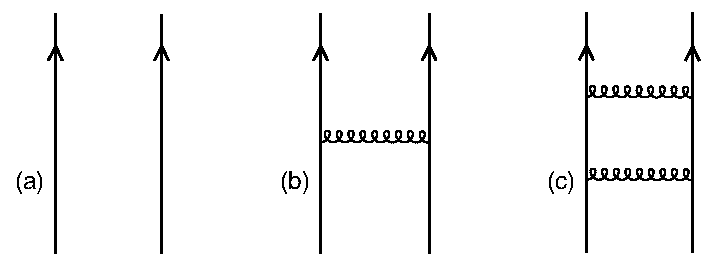
\includegraphics[width=0.8\linewidth]{figures/fig_1_1.pdf}
\caption{(a) 自由に伝播する二つの粒子。(b) 1個の重力子の交換による補正。(c) 2個の重力子の交換による補正。}
\label{fig:1.1}
\end{figure}

この次元解析から直ちに、量子重力による補正が非関連相互作用であることがわかる。これは、低エネルギーでは弱くなり、とくに数百 $\mathrm{GeV}$ という素粒子物理のエネルギーでは無視できることを意味する。同じ理由から、高エネルギーでは結合が強くなり、$E>M_{\mathrm P}$ では摂動論が破綻する。図\hyperref[fig:1.1]{1.1}(c)の重力子2個による補正では、中間状態について和をとる。エネルギーの高い $E'$ の中間状態については、次元の考察から、重力子2個の振幅と重力子0個の振幅との比は
\begin{equation}
G_{\mathrm N}^{\,2}E^2\int dE'\,E'
=\frac{E^2}{M_{\mathrm P}^{\,4}}\int dE'\,E'
\tag{1.1.3}\label{eq:1.1.3}
\end{equation}
程度となる。理論を任意に高いエネルギーまで外挿すると、これは発散する。位置空間では、この発散は、すべての重力子の頂点が一致する極限から生じる。重力子を一つ追加するごとに発散は悪化する。これが繰り込み不可能性の問題である。

考えられる解決は二つある。第一は、発散が相互作用のべきで展開することによって生じており、理論を厳密に扱えば消えるというものである。繰り込み群の言葉では、これは非自明な紫外固定点に対応する。第二は、理論を任意に高いエネルギーまで外挿することが誤りであり、あるエネルギーを超えると、時空内で相互作用を広げて発散を和らげるように理論が修正されるというものである。量子重力が非自明な紫外固定点をもつかどうかは知られていないが、第二の可能性に注目する理由はいくつもある。一つは歴史である。弱い相互作用の Fermi 理論における同種の発散問題は、新しい物理の兆候であった。フェルミオン間の接触相互作用が、より短い距離ではゲージボソンの交換として分解されたのである。もう一つは、標準模型の構成を説明するために、いずれにせよより完全な理論が必要であり、その同じ新しい物理が量子重力の発散問題も解決すると期待するのは妥当だということである。

場の量子論では、理論の整合性を保ちながら相互作用を広げることは容易でない。Lorentz 不変性が非常によい近似で成り立つことはわかっている。このことは、空間内で相互作用を広げれば時間内でも広げることになり、その結果、因果律あるいはユニタリティが失われることを意味する。さらに、Lorentz 不変性が実際には局所対称性である一般座標不変性に組み込まれていることもわかっており、これによって、不整合を生じさせずに相互作用を広げることは、いっそう難しくなる。

実際、理論の整合性を損なうことなく重力相互作用を広げ、発散を切り捨てる方法として、現在知られているものは一つしかない。それが、図\hyperref[fig:1.2]{1.2}に示す弦理論である。この理論では、重力子と他のすべての素粒子は、場の量子論のような点ではなく、一次元の物体である弦である。なぜこれがうまくいき、他のものではいけないのかは、先験的にはまったく明らかでないが、理論を展開していくにつれ、その仕組みがわかるであろう。\footnote[1]{少なくとも一つのよくある疑問、すなわちなぜ膜、つまり二次元以上の物体ではいけないのか、という疑問には直観的な答えがある。粒子をより多くの次元に広げると、時空の発散は軽減されるが、内部自由度の数の増大に由来する新しい発散に遭遇するのである。時空の発散と内部の発散の両方を制御できるのは、一次元の場合に限られるように見える。ただし、第14章で議論するように、膜という考えは、やや姿を変えて行列理論として再登場している。}
われわれには単に想像力が足りないだけであり、短距離カットオフをもつ整合的な重力理論は、ほかにも多数あるのかもしれない。しかし、場の量子論における発散問題は簡単には解決されないということを経験は示している。したがって、解決法が一つでもあるなら、それをきわめて真剣に受け止めるべきである。実際、整合性という原理がこれほど強い制約を与えることがわかったのは、幸いである。重力と他の相互作用の統一は $M_{\mathrm P}$ という非常に高いエネルギーで起こるため、実験的検証は難しく、間接的なものになるからである。

\begin{figure}[htbp]
\centering
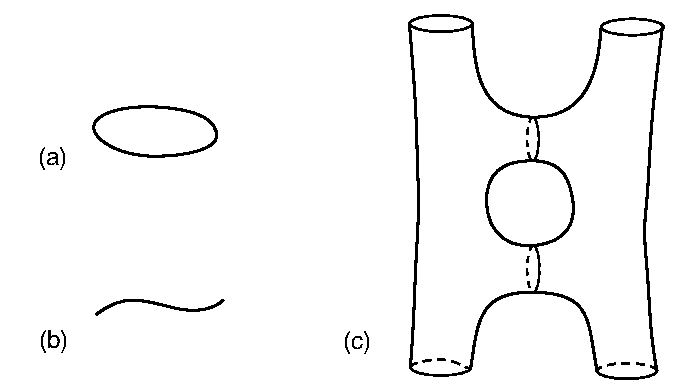
\includegraphics[width=0.8\linewidth]{figures/fig_1_2.pdf}
\caption{(a) 閉弦。(b) 開弦。(c) 弦理論における図\hyperref[fig:1.1]{1.1}(c)のループ振幅。各粒子の世界線は円筒となり、相互作用はもはや点で起こらない。（中間の線に描いた断面は、立体的な形状をわかりやすくするためだけに加えたものである。）}
\label{fig:1.2}
\end{figure}

では、この考えを追求すると何が見いだされるだろうか。一言でいえば、驚くべき結果が得られる。弦理論は、標準模型の構成を説明するための従来の考えと見事にかみ合い、しかも、場の量子論に比べていっそう優美で統一された構造のもとで、それを実現する。とくに、一次元の物体について整合的な相対論的量子論を構成しようとすると、次のことがわかる。
\begin{enumerate}
\item 重力。整合的な弦理論はすべて、質量のないスピン2の状態を含まなければならず、その相互作用は低エネルギーで一般相対論に帰着する。
\item 少なくとも摂動論の範囲では、整合的な量子重力理論。すでに述べたように、これは既知のすべての重力の場の量子論と対照的である。
\item 大統一。弦理論は、標準模型を含むのに十分大きいゲージ群を導く。最も単純な弦理論のいくつかは、標準模型の統一に現れるのと同じゲージ群とフェルミオン表現を導く。
\item 余剰次元。弦理論は、時空の次元が10という特定の数であることを要求する。\footnote[2]{正確にいうと、弦理論は時空の位相と幾何の概念を修正するので、ここで次元と呼ぶものは一般化されたものである。また、10次元は弱結合の弦理論にとって適切な数であるが、強結合では描像が変わりうることを見るであろう。}
場の方程式には、大きく平坦な四つの次元と、小さく曲がった六つの次元をもち、四次元の物理が標準模型に似ている解が存在する。
\item 超対称性。整合的な弦理論は、顕在的な対称性、または自発的に破れた対称性として、時空の超対称性を必要とする。
\item カイラルなゲージ結合。自然界のゲージ相互作用は、パリティに関して非対称、すなわちカイラルである。このことは、従来の統一の考えのいくつかにとって障害であった。それらはパリティ対称なゲージ結合を必要としていたからである。弦理論ではカイラルなゲージ結合が許される。
\item 自由パラメータがない。弦理論には調整可能な定数が存在しない。
\item 一意性。連続的なパラメータが存在しないだけでなく、場の理論におけるゲージ群や表現の選択に相当する離散的な自由も存在しない。弦理論は一意である。
\end{enumerate}
加えて、アクシオンや隠れたゲージ群など、統一の考えの中で役割を果たしてきた、ほかの多くの特徴も見いだされる。

これは、一次元の物体という単純な仮定から生じるものとして、驚くべき一覧である。最初の二項だけでも大いに興味深い。その次の四項は、標準模型を統一しようとするときに到達する描像に、驚くほど近い。そして最後の二項が示すように、弦理論は、場の量子論よりも緊密で恣意性の少ない構造によってこれを実現し、それまでの考えに欠けていた要素を与える。最初の項も、この構造の緊密さのさらなる例である。弦理論には重力子が必ず存在しなければならないのに対し、場の理論では、重力子や他の場は個別に選んで組み合わされる。

さらに、弦理論は数学の多くの分野と結びついており、それらの間に新しく予想外の関係を見いだすことにつながってきた。また、超対称な場の量子論における近年の発見と豊かな関係をもつ。弦理論は、量子重力のより深い問題の一部、とくにブラックホールの量子力学にも取り組み始めている。

もちろん、なすべきことは多く残っている。弦理論は、大筋では現実の世界に似ているかもしれないが、決定的な検証はなお遠いように思われる。主な問題は、理論は一意であるにもかかわらず、大きく平坦な四つの次元をもつ解に注意を限っても、膨大な数の古典解が存在することである。量子化すると、これらはそれぞれ理論の可能な基底状態、すなわち真空となり、各々で四次元の物理は異なる。量子効果によって安定な解の数が大きく減ることは知られているが、力学の完全な理解はいまだ得られていない。

標準模型においてさえ、真空の力学が、われわれの観測する物理で重要な役割を果たすことを思い起こしておこう。電弱相互作用では、真空の対称性が Hamiltonian の対称性より低いという事実、すなわち対称性の自発的破れが中心的な役割を果たす。強い相互作用では、真空中の大きく揺らぐゲージ場がクォークの閉じ込めをもたらす。場の量子論におけるこれらの現象は、多数の自由度をもつ量子系であることから生じる。弦理論には、はるかに多くの自由度があるように見えるため、さらに豊かな力学を期待すべきである。

さらに、「弦理論とは何か」という問題がある。つい最近まで、弦理論についてのわれわれの理解は、少数の弦が弱く相互作用する摂動論に限られていた。強結合において、理論をどのように定義すればよいのかさえ知られていなかった。弱結合で用いる自由度である一次元の物体は、究極的には、理論を理解するための最も単純で、最も完全な方法ではないのではないか、という疑いがあった。

過去数年間、これらの問題には大きな進展があった。その多くは、超対称性が課す制約を系統的に適用することから生まれた。強結合の弦の力学を完全に理解したわけでは決してないが、十分な量の超対称性が破れずに残っている場合には、真空の空間を詳細に描き出すことが可能になり、それは多くの驚きをもたらした。一つは、理論の絶対的な一意性である。弱結合の弦理論はいくつか存在するが、そのすべてが、単一の理論の真空の空間における極限であることがわかった。もう一つは、時空が11次元になる極限である。11という数は、超重力の観点からは興味深いが、弱結合の弦理論では不可能な数である。また、この理論には D-brane という新しい広がりをもつ物体が含まれることも理解され、これがブラックホールの量子力学の新しい理解につながった。これらすべては、理論の究極的な姿についても、新しく予想外の手掛かりを与えている。

まとめると、これほど多くのアプローチが、一つの有力な考えへと収束するように見えるのは幸いである。量子重力の発散問題から出発しても、標準模型の構成を説明しようとする試みから出発しても、あるいは統一理論の構成に役立ちうる新たな対称性や数学的構造の探求から出発しても、弦理論へ導かれるのである。

\subsubsectionlink*{本書の構成}

この全2巻の目標は、弦理論を初歩から始め、四次元へのコンパクト化、そして強結合の弦に関する最新の進展にまで進む、完全な入門を提供することである。

第1巻は、ボソン弦理論への入門である。これは現実的な理論ではない。フェルミオンをもたず、知られている限り、安定な基底状態ももたない。ここでの考え方は、場の量子論の講義をスカラー場の理論の徹底的な学習から始める場合と同じである。スカラー場の理論も、最終的に関心のある理論ではないが、スピンやゲージ不変性に伴う複雑さを導入する前に、場の量子論に特有の力学的・技術的な特徴を展開するための単純な例を与える。同様に、ボソン弦理論を十分に学ぶことで、フェルミオンと超対称性に伴う追加の複雑さを短い手順で組み込める枠組みが得られる。

第1章の残りは導入である。まず、弦の力学に対する作用原理を提示する。次に、光円錐ゲージを用いて、手早く直観的に量子化を行い、弦のスペクトルの重要な側面のいくつかを示す。第2章から第7章までは、ボソン弦理論の基礎的な入門である。第2章では、共形不変性、演算子積展開、頂点演算子など、世界面の場の量子論で必要な技術的道具を導入する。第3章と第4章では、Polyakov の経路積分から出発して弦の共変量子化を行う。第5章から第7章では相互作用を扱い、一般的な形式を提示したのち、それを木のレベルと1ループの振幅に適用する。第8章では、いくつかの次元を周期的にするという、弦理論の最も単純なコンパクト化を扱う。Kaluza--Klein ゲージ対称性など、コンパクト化された場の理論で生じる現象に加えて、拡大されたゲージ対称性、$T$ 双対性、D-brane など、豊富な「弦特有の」物理もある。第9章では、高次の振幅を扱う。前半では、先に述べたとおり弦理論が摂動論において有限かつユニタリであるという議論の概略を示す。後半では、弦の場の理論など、いくつかの発展的な話題を簡潔に扱う。付録Aは経路積分への入門であり、これにより、本書における場の量子論の使用を自己完結したものにする。

第2巻では、超対称な弦理論を扱う。まず10次元などの対称性の高い真空に注目し、その後、現実的な四次元の真空を扱う。

第10章から第12章では、それまでの導入を超対称な弦理論へ拡張し、I型、II型、ヘテロティック超弦とその相互作用を展開する。その後、これらの主題に関する最新の結果を導入する。第13章では、本書でそれまでに展開した弦の摂動論の道具を引き続き用いて、D-brane の性質と力学を論じる。続く第14章では、超対称性に基づく議論を用いて強結合の弦を理解する。任意の弦理論の強結合極限は、双対な弱結合の弦理論、あるいは暫定的に M理論と呼ばれる新しい11次元の理論によって記述されることを見る。弦理論の完全な定式化の探求がどの段階にあるかを議論し、一つの有望な考えである m(atrix) 理論を紹介する。また、最も単純なエントロピー計算を行い、ブラックホールの量子力学を簡潔に論じる。第15章では、さまざまな世界面対称性代数の発展的な応用をまとめる。

第16章と第17章では、オービフォールド・コンパクト化と Calabi--Yau コンパクト化に基づく四次元の弦理論を提示する。目標は網羅的に扱うことではなく、最も単純な例を標準模型の統一と結びつけることである。第18章では、世界面と時空のゲージ対称性に基づく一般的な議論を用いて、広いクラスの弦理論で成り立つ結果をまとめる。第19章は発展的な話題からなり、$(2,2)$ 世界面超対称性、ミラー対称性、コニフォールド転移、およびいくつかのコンパクト化された理論の強結合での振る舞いを含む。

各巻の末尾には、注釈付きの参考文献一覧を置いた。学習者に役立ちそうな論文、とりわけ総説を選んで集めるよう努めた。各巻の末尾には用語集も付してある。

\subsectionlink{作用原理}\label{sec:1.2}

一次元の物体、すなわち弦の古典力学と量子力学を調べたい。弦は $D$ 次元の平坦な時空内を運動し、その計量は $\eta_{\mu\nu}=\operatorname{diag}(-,+,+,\ldots,+)$ である。

まず、零次元の物体である相対論的な点粒子の古典力学を復習しておくと便利である。粒子の運動は、その位置を、時間の $D-1$ 個の関数 $\mathbf X(X^0)$ として与えることで記述できる。しかし、これでは理論の共変性が隠れてしまうため、粒子の世界線に沿ってパラメータ $\tau$ を導入し、時空内の運動を $D$ 個の関数 $X^\mu(\tau)$ によって記述する方がよい。パラメータ表示は任意である。同じ経路の異なるパラメータ表示は物理的に等価であり、すべての物理量はこの選択に依存してはならない。すなわち、任意の単調関数 $\tau'(\tau)$ に対し、
\begin{equation}
X'^\mu\bigl(\tau'(\tau)\bigr)=X^\mu(\tau)
\tag{1.2.1}\label{eq:1.2.1}
\end{equation}
で与えられる二つの経路 $X'^\mu$ と $X^\mu$ は同じものである。対称性の低い記述を、より対称だが冗長な記述に置き換えているわけであり、これはしばしば有用な手順となる。図\hyperref[fig:1.3]{1.3}(a)に、パラメータ表示した世界線を示す。

\begin{figure}[htbp]
\centering
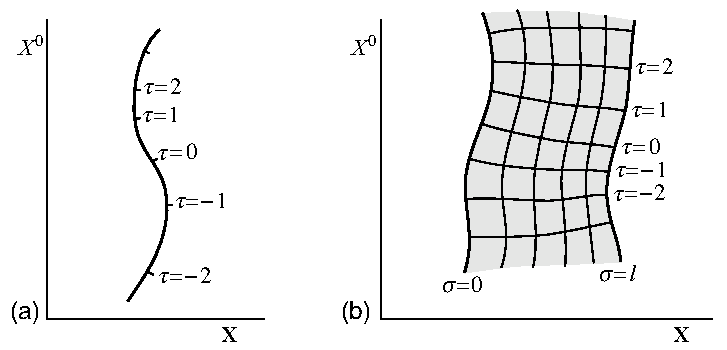
\includegraphics[width=0.8\linewidth]{figures/fig_1_3.pdf}
\caption{(a) パラメータ表示した点粒子の世界線。(b) パラメータ表示した開弦の世界面。}
\label{fig:1.3}
\end{figure}

パラメータ表示に依存しない、最も単純な Poincaré 不変な作用は、世界線に沿う固有時に比例するものであろう。
\begin{equation}
S_{\mathrm{pp}}=-m\int d\tau\,(-\dot X^\mu\dot X_\mu)^{1/2}.
\tag{1.2.2}\label{eq:1.2.2}
\end{equation}
ここで、ドットは $\tau$ に関する微分を表す。部分積分すると、作用の変分は
\begin{equation}
\delta S_{\mathrm{pp}}=-m\int d\tau\,\dot u_\mu\,\delta X^\mu
\tag{1.2.3}\label{eq:1.2.3}
\end{equation}
となる。ただし、
\begin{equation}
u^\mu=\dot X^\mu(-\dot X^\nu\dot X_\nu)^{-1/2}
\tag{1.2.4}\label{eq:1.2.4}
\end{equation}
は規格化された $D$ 元速度である。したがって、運動方程式 $\dot u^\mu=0$ は自由運動を記述する。非相対論的極限を見ることで確認できるように、規格化定数 $m$ は粒子の質量である（演習1.1）。

世界線上に追加の場、すなわち独立な世界線計量 $\gamma_{\tau\tau}(\tau)$ を導入すれば、作用をもう一つの便利な形に書ける。正であると定義したテトラッド $\eta(\tau)=(-\gamma_{\tau\tau}(\tau))^{1/2}$ を用いると便利である。テトラッドという語の語根は「四」を意味するが、ここでは一般相対論のこの用語を任意の次元数で用いる。このとき
\begin{equation}
S'_{\mathrm{pp}}=\frac12\int d\tau\,
\bigl(\eta^{-1}\dot X^\mu\dot X_\mu-\eta m^2\bigr).
\tag{1.2.5}\label{eq:1.2.5}
\end{equation}
この作用は、先ほどの作用 $S_{\mathrm{pp}}$ と同じ対称性、すなわち Poincaré 不変性と世界線の再パラメータ化不変性をもつ。後者の下で $\eta(\tau)$ は
\begin{equation}
\eta'(\tau')\,d\tau'=\eta(\tau)\,d\tau
\tag{1.2.6}\label{eq:1.2.6}
\end{equation}
と変換する。

テトラッドを変分して得られる運動方程式は
\begin{equation}
\eta^2=-\dot X^\mu\dot X_\mu/m^2
\tag{1.2.7}\label{eq:1.2.7}
\end{equation}
である。これを用いて $\eta(\tau)$ を消去すると、作用 $S'_{\mathrm{pp}}$ は先ほどの $S_{\mathrm{pp}}$ となる。ちなみに、$S'_{\mathrm{pp}}$ は質量のない粒子に対してもまったく問題なく意味をもつが、その場合 $S_{\mathrm{pp}}$ は使えない。

作用 $S_{\mathrm{pp}}$ と $S'_{\mathrm{pp}}$ は古典的には等価であるが、$S_{\mathrm{pp}}$ は微分を平方根の内部に含む複雑な形をしているため、経路積分の中で意味を与えることが難しい。一方、$S'_{\mathrm{pp}}$ は微分について二次であり、その経路積分は、後の章で見るように、かなり容易に評価できる。おそらく、$S_{\mathrm{pp}}$ に対して量子論を定義しようとするどのような試みも、$S'_{\mathrm{pp}}$ の経路積分と等価な結果へ至るであろう。そこで、後者を量子論の定義の出発点とする。

一次元の物体は、図\hyperref[fig:1.3]{1.3}(b)のように、二つのパラメータを用いた $X^\mu(\tau,\sigma)$ によって記述できる二次元の世界面を描く。粒子の場合と同様、作用などの物理量は、時空への埋め込みのみに依存し、パラメータ表示には依存しないことを要求する。理論がこの性質をもつことは魅力的であるばかりでなく、整合的な相対論的量子論には必要であることも見るであろう。最も単純な不変作用である Nambu--Goto 作用は、世界面の面積に比例する。この作用を $X^\mu(\tau,\sigma)$ によって表すため、まず誘導計量 $h_{ab}$ を定義する。添字 $a,b,\ldots$ は $(\tau,\sigma)$ の値をとる。
\begin{equation}
h_{ab}=\partial_aX^\mu\partial_bX_\mu.
\tag{1.2.8}\label{eq:1.2.8}
\end{equation}
すると Nambu--Goto 作用は
\begin{align}
S_{\mathrm{NG}}&=\int_M d\tau\,d\sigma\,\mathcal L_{\mathrm{NG}},
\tag{1.2.9a}\label{eq:1.2.9a}\\
\mathcal L_{\mathrm{NG}}&=-\frac{1}{2\pi\alpha'}(-\det h_{ab})^{1/2}
\tag{1.2.9b}\label{eq:1.2.9b}
\end{align}
となる。ここで $M$ は世界面を表す。時空の長さの二乗の単位をもつ定数 $\alpha'$ は Regge 勾配であり、その意味は後で明らかになる。弦の張力 $T$ と Regge 勾配の関係は
\begin{equation}
T=\frac{1}{2\pi\alpha'}
\tag{1.2.10}\label{eq:1.2.10}
\end{equation}
である（演習1.1）。

次に、作用の対称性、すなわち $S_{\mathrm{NG}}[X']=S_{\mathrm{NG}}[X]$ となる $X^\mu(\tau,\sigma)$ の変換を考えよう。これらは次のものである。
\begin{enumerate}
\item 平坦な時空の等長変換群、すなわち $D$ 次元 Poincaré 群：
\begin{equation}
X'^\mu(\tau,\sigma)=\Lambda^\mu{}_\nu X^\nu(\tau,\sigma)+a^\mu.
\tag{1.2.11}\label{eq:1.2.11}
\end{equation}
ここで $\Lambda^\mu{}_\nu$ は Lorentz 変換、$a^\mu$ は並進である。
\item 二次元の座標不変性。しばしば微分同相（diff）不変性と呼ばれる。新しい座標 $(\tau'(\tau,\sigma),\sigma'(\tau,\sigma))$ に対し、変換は
\begin{equation}
X'^\mu(\tau',\sigma')=X^\mu(\tau,\sigma)
\tag{1.2.12}\label{eq:1.2.12}
\end{equation}
である。
\end{enumerate}

Nambu--Goto 作用は、平方根の中に微分を含む点で、点粒子の作用 $S_{\mathrm{pp}}$ に類似している。ここでも、独立な世界面計量 $\gamma_{ab}(\tau,\sigma)$ を導入することによって単純化できる。以下では、「誘導」と明示しない限り、「計量」は常に $\gamma_{ab}$ を意味し、添字の上げ下げも常にこの計量を用いて行う。$\gamma_{ab}$ は Lorentz 型の符号 $(-,+)$ をもつものとする。作用は
\begin{equation}
S_{\mathrm P}[X,\gamma]=-\frac{1}{4\pi\alpha'}
\int_M d\tau\,d\sigma\,(-\gamma)^{1/2}\gamma^{ab}
\partial_aX^\mu\partial_bX_\mu
\tag{1.2.13}\label{eq:1.2.13}
\end{equation}
であり、$\gamma=\det\gamma_{ab}$ である。これは Brink--Di Vecchia--Howe--Deser--Zumino 作用、略して Polyakov 作用である。Brink、Di Vecchia、Howe、および Deser と Zumino が、世界面の局所超対称性をもつ一般化を導く過程で見いだした。その利点、とくに経路積分量子化における利点を強調したのは Polyakov である。

$S_{\mathrm{NG}}$ との等価性を見るため、計量を変分して得られる運動方程式を用いる。
\begin{equation}
\delta_\gamma S_{\mathrm P}[X,\gamma]=-\frac{1}{4\pi\alpha'}
\int_M d\tau\,d\sigma\,(-\gamma)^{1/2}\delta\gamma^{ab}
\left(h_{ab}-\frac12\gamma_{ab}\gamma^{cd}h_{cd}\right).
\tag{1.2.14}\label{eq:1.2.14}
\end{equation}
ここで $h_{ab}$ は、やはり誘導計量\hyperref[eq:1.2.8]{(1.2.8)}である。行列式の変分に関する一般的な関係
\begin{equation}
\delta\gamma=\gamma\gamma^{ab}\delta\gamma_{ab}
=-\gamma\gamma_{ab}\delta\gamma^{ab}
\tag{1.2.15}\label{eq:1.2.15}
\end{equation}
を用いた。すると、$\delta_\gamma S_{\mathrm P}=0$ は
\begin{equation}
h_{ab}=\frac12\gamma_{ab}\gamma^{cd}h_{cd}
\tag{1.2.16}\label{eq:1.2.16}
\end{equation}
を意味する。この方程式を、その行列式にマイナスを付けたものの平方根で割ると、
\begin{equation}
h_{ab}(-h)^{-1/2}=\gamma_{ab}(-\gamma)^{-1/2}
\tag{1.2.17}\label{eq:1.2.17}
\end{equation}
が得られる。したがって、$\gamma_{ab}$ は誘導計量に比例する。さらにこれを用いて、作用から $\gamma_{ab}$ を消去できる。
\begin{equation}
S_{\mathrm P}[X,\gamma]\longrightarrow
-\frac{1}{2\pi\alpha'}\int d\tau\,d\sigma\,(-h)^{1/2}
=S_{\mathrm{NG}}[X].
\tag{1.2.18}\label{eq:1.2.18}
\end{equation}

作用 $S_{\mathrm P}$ は、次の対称性をもつ。
\begin{enumerate}
\item $D$ 次元 Poincaré 不変性：
\begin{equation}
\begin{aligned}
X'^\mu(\tau,\sigma)&=\Lambda^\mu{}_\nu X^\nu(\tau,\sigma)+a^\mu,\\
\gamma'_{ab}(\tau,\sigma)&=\gamma_{ab}(\tau,\sigma).
\end{aligned}
\tag{1.2.19}\label{eq:1.2.19}
\end{equation}
\item 微分同相不変性：
\begin{equation}
\begin{aligned}
X'^\mu(\tau',\sigma')&=X^\mu(\tau,\sigma),\\
\frac{\partial\sigma'^c}{\partial\sigma^a}
\frac{\partial\sigma'^d}{\partial\sigma^b}\gamma'_{cd}(\tau',\sigma')
&=\gamma_{ab}(\tau,\sigma),
\end{aligned}
\tag{1.2.20}\label{eq:1.2.20}
\end{equation}
ここで $\sigma'^a(\tau,\sigma)$ は新しい座標である。
\item 二次元 Weyl 不変性：
\begin{equation}
\begin{aligned}
X'^\mu(\tau,\sigma)&=X^\mu(\tau,\sigma),\\
\gamma'_{ab}(\tau,\sigma)&=\exp\bigl(2\omega(\tau,\sigma)\bigr)
\gamma_{ab}(\tau,\sigma),
\end{aligned}
\tag{1.2.21}\label{eq:1.2.21}
\end{equation}
ここで $\omega(\tau,\sigma)$ は任意である。
\end{enumerate}
世界面計量の局所的なスケール変換である Weyl 不変性に相当するものは、Nambu--Goto の形式にはない。それが現れる理由は、Polyakov 作用と Nambu--Goto 作用を結びつけるのに用いた運動方程式\hyperref[eq:1.2.17]{(1.2.17)}を振り返ることで理解できる。この式は $\gamma_{ab}$ を完全には決めず、局所的なスケール変換の自由度を残してしか決めない。そのため、Weyl 変換で等価な計量は、時空への同じ埋め込みに対応する。これは、明らかな微分同相不変性に加えて、Polyakov の定式化がもつ追加の冗長性である。

計量に関する作用の変分によって、エネルギー運動量テンソルを定義する。
\begin{equation}
\begin{aligned}
T^{ab}(\tau,\sigma)&=-4\pi(-\gamma)^{-1/2}
\frac{\delta}{\delta\gamma_{ab}}S_{\mathrm P}\\
&=-\frac{1}{\alpha'}\left(
\partial^aX^\mu\partial^bX_\mu
-\frac12\gamma^{ab}\partial_cX^\mu\partial^cX_\mu\right).
\end{aligned}
\tag{1.2.22}\label{eq:1.2.22}
\end{equation}
これは、場の理論における通常の定義に比べて $-2\pi$ という余分な因子をもつ。弦理論では、これが標準的で便利な規約である。微分同相不変性の帰結として、これは保存する：$\nabla_aT^{ab}=0$。さらに、任意の Weyl 変換に対する $S_{\mathrm P}$ の不変性は、
\begin{equation}
\gamma_{ab}\frac{\delta}{\delta\gamma_{ab}}S_{\mathrm P}=0
\quad\Rightarrow\quad T^a{}_a=0
\tag{1.2.23}\label{eq:1.2.23}
\end{equation}
を意味する。

作用 $S_{\mathrm{NG}}$ と $S_{\mathrm P}$ は、弦の世界面上の二次元場の理論を定義する。弦理論では、時空内の過程の振幅が、世界面上の二次元場の量子論における行列要素によって与えられることを見るであろう。われわれの関心は四次元時空にあるが、弦の摂動論で用いる道具の大部分は二次元のものである。世界面の観点では、座標変換則\hyperref[eq:1.2.12]{(1.2.12)}は $X^\mu(\tau,\sigma)$ をスカラー場と定義しており、$\mu$ は内部添字として付随している。二次元の観点からは、Polyakov 作用は計量 $\gamma_{ab}$ に共変的に結合した、質量のない Klein--Gordon スカラー $X^\mu$ を記述する。また、この観点では Poincaré 不変性は内部対称性である。すなわち、$\tau,\sigma$ を固定した場に作用する。

作用で $\gamma_{ab}$ を変分すると、運動方程式
\begin{equation}
T_{ab}=0
\tag{1.2.24}\label{eq:1.2.24}
\end{equation}
が得られる。$X^\mu$ を変分すると、運動方程式
\begin{equation}
\partial_a\bigl[(-\gamma)^{1/2}\gamma^{ab}\partial_bX^\mu\bigr]
=(-\gamma)^{1/2}\nabla^2X^\mu=0
\tag{1.2.25}\label{eq:1.2.25}
\end{equation}
が得られる。境界をもつ世界面では、作用の変分に表面項も現れる。具体的に、座標領域を
\begin{equation}
-\infty<\tau<\infty,\qquad 0\leq\sigma\leq\ell
\tag{1.2.26}\label{eq:1.2.26}
\end{equation}
としよう。$\tau$ を時間変数、$\sigma$ を空間的な変数と考えるので、これは源なしで伝播する一本の弦である。このとき
\begin{equation}
\begin{aligned}
\delta S_{\mathrm P}
={}&\frac{1}{2\pi\alpha'}\int_{-\infty}^{\infty}d\tau
\int_0^\ell d\sigma\,(-\gamma)^{1/2}\delta X^\mu\nabla^2X_\mu\\
&-\frac{1}{2\pi\alpha'}\int_{-\infty}^{\infty}d\tau\,
\left.(-\gamma)^{1/2}\delta X^\mu\partial^\sigma X_\mu
\right|_{\sigma=0}^{\sigma=\ell}.
\end{aligned}
\tag{1.2.27}\label{eq:1.2.27}
\end{equation}
内部では、運動方程式は先ほどと同じである。
\begin{equation}
\partial^\sigma X^\mu(\tau,0)=\partial^\sigma X^\mu(\tau,\ell)=0
\tag{1.2.28}\label{eq:1.2.28}
\end{equation}
ならば、境界項は消える。これらは $X^\mu$ に対する Neumann 境界条件である。より共変的に述べると、
\begin{equation}
n^a\partial_aX_\mu=0\qquad \text{$\partial M$ 上で}
\tag{1.2.29}\label{eq:1.2.29}
\end{equation}
となる。ここで $n^a$ は境界 $\partial M$ に垂直である。開弦の両端は、時空内を自由に動く。

また、
\begin{align}
X^\mu(\tau,\ell)&=X^\mu(\tau,0),&
\partial^\sigma X^\mu(\tau,\ell)&=\partial^\sigma X^\mu(\tau,0),
\tag{1.2.30a}\label{eq:1.2.30a}\\
\gamma_{ab}(\tau,\ell)&=\gamma_{ab}(\tau,0)
\tag{1.2.30b}\label{eq:1.2.30b}
\end{align}
を課しても、運動方程式の表面項は消える。つまり、場は周期的である。境界は存在せず、両端は結び合わされて閉じた輪をなす。

開弦の境界条件\hyperref[eq:1.2.28]{(1.2.28)}と閉弦の境界条件\hyperref[eq:1.2.30a]{(1.2.30)}が、$D$ 次元 Poincaré 不変性および運動方程式と両立する唯一の可能性である。Poincaré 不変性の条件を緩めると、ほかの可能性もあり、後に重要になる。その一部は演習で調べる。

Nambu--Goto 作用と Polyakov 作用は、与えられた対称性をもつ最も単純な作用かもしれない。しかし、作用の単純さは、場の量子論における正しい基準ではない。鍵となる考えは、単純さではなく対称性である。物理的理由と技術的理由の両方から、通常は理論のすべての対称性と両立する最も一般的な局所作用を考えねばならない。対称性が保たれ、作用が微分の多項式であることを要求して、Polyakov 作用を一般化してみよう（そうでなければ量子論に意味を与えることが難しい）。\footnote[3]{この要請を緩めると、誘導計量 $h_{ab}$ の曲率から構成される不変量など、さまざまな追加の可能性が生じる。電束管や磁束管のような一次元の物体では、そのような項が現れると予想され、その場合は物体の太さがカットオフを与えるため、経路積分は意味をもつ。しかし、基礎的な弦理論で扱うような、無限に細い弦ではこれは不可能である。}
大域的な Weyl 不変性、すなわち $\omega(\tau,\sigma)=\text{定数}$ は、$(-\gamma)^{1/2}$ の変化を打ち消すために、作用において $\gamma^{ab}$ の因子の数が $\gamma_{ab}$ の因子の数より一つ多いことを要求する。余った上付き添字は微分としか縮約できないため、各項は正確に二つの微分を含む。すると、座標不変性と Poincaré 不変性から、元の $S_{\mathrm P}$ に加えて、次の一つの項が許される。
\begin{equation}
\chi=\frac{1}{4\pi}\int_M d\tau\,d\sigma\,(-\gamma)^{1/2}R.
\tag{1.2.31}\label{eq:1.2.31}
\end{equation}
ここで $R$ は、$\gamma_{ab}$ から構成される Ricci スカラーである。局所的な Weyl スケール変換の下で、
\begin{equation}
(-\gamma')^{1/2}R'=(-\gamma)^{1/2}\bigl(R-2\nabla^2\omega\bigr).
\tag{1.2.32}\label{eq:1.2.32}
\end{equation}
任意の $v^a$ に対し $(-\gamma)^{1/2}\nabla_av^a
=\partial_a\bigl((-\gamma)^{1/2}v^a\bigr)$ であるため、この変分は全微分である。したがって積分\hyperref[eq:1.2.31]{(1.2.31)}は、境界をもたない世界面では不変である。境界がある場合には、追加の表面項が必要となる（演習1.3）。

$\chi$ は対称性によって許されるので、作用に含めることにする。
\begin{equation}
\begin{aligned}
S'_{\mathrm P}&=S_{\mathrm P}-\lambda\chi\\
&=-\int_M d\tau\,d\sigma\,(-\gamma)^{1/2}
\left(\frac{1}{4\pi\alpha'}\gamma^{ab}\partial_aX^\mu\partial_bX_\mu
+\frac{\lambda}{4\pi}R\right).
\end{aligned}
\tag{1.2.33}\label{eq:1.2.33}
\end{equation}
これは、これらの場と対称性のもとで、$(\text{diff}\times\text{Weyl})$ 不変かつ Poincaré 不変な最も一般的な作用である。当面、対称性についての議論は古典的なものであり、量子異常の可能性は無視している。それについては第3章で考察する。

作用 $S'_{\mathrm P}$ は、計量に対する Hilbert 作用 $\int(-\gamma)^{1/2}R$ に、$D$ 個の質量のないスカラー場 $X^\mu$ を最小結合したものに見える。しかし二次元では、Hilbert 作用は世界面の位相のみに依存し、計量に力学を与えない。このことを見るため、その変分が $R_{ab}-\tfrac12\gamma_{ab}R$ に比例するという一般相対論の結果を用いる。二次元では、曲率テンソルの対称性から $R_{ab}=\tfrac12\gamma_{ab}R$ が従うため、これはゼロになる。すなわち、Hilbert 作用は計量の任意の連続変化に対して不変である。ただし、第3章で見るように、何らかの大域的な意味はもっている。

理論をさらに一般化しようとする方法はいろいろある。一つは、最終的な関心が $D=4$ にあることに示唆されるもので、$X^\mu$ 場を四つより多く許しつつ、四次元 Poincaré 不変性だけを要求するというものである。第二は、対称性こそが最も重要であるという考えに動機づけられるもので、同じ局所対称性と四次元 Poincaré 不変性を保ちつつ、より一般的な場の内容を許すというものである。すなわち、世界面および時空の対称群の異なる表現に属する二次元の場を許す。これらの考えはいずれも重要であり、さまざまな機会に立ち戻ることになる。さらに別の考えは、理論の局所対称性を拡大することであり、第2巻ではこの考えを追求する。

\subsectionlink{開弦のスペクトル}
\label{sec:1.3}

この節では開弦のスペクトルを、次の節では閉弦のスペクトルを論じる。その際、光円錐ゲージを用いて $\mathrm{diff}\times\mathrm{Weyl}$ の冗長性を除く。このゲージは理論の共変性を見えなくするが、スペクトルへ至る最短の方法であり、臨界次元や質量ゼロのゲージ粒子の存在といった重要な特徴を明らかにする。ここでは方法よりも結果に重点を置くので、読者は細部にこだわる必要はない。共変な共形ゲージを用いた系統的な取り扱いは次章から始める。

時空に光円錐座標を定義する：
\begin{equation}
x^\pm=2^{-1/2}(x^0\pm x^1),\qquad x^i,\quad i=2,\ldots,D-1.
\tag{1.3.1}\label{eq:1.3.1}
\end{equation}
時空座標 $x^\mu$ には小文字を、それに対応する世界面上の場 $X^\mu(\sigma,\tau)$ には大文字を用いている。この座標での計量は
\begin{align}
a^\mu b_\mu&=-a^+b^- -a^-b^+ +a^ib^i,
\tag{1.3.2a}\label{eq:1.3.2a}\\
a_-&=-a^+,\qquad a_+=-a^-,\qquad a_i=a^i.
\tag{1.3.2b}\label{eq:1.3.2b}
\end{align}
世界面の各点で、世界面のパラメーター $\tau$ を時空座標 $x^+$ に等しく取る。$\tau=x^0$ を試そうと思うかもしれないが、それでは同じような簡単化は得られない。したがって、$x^+$ が時間の役割を、$p^-$ がエネルギーの役割を果たす。縦方向の変数 $x^-$ と $p^+$ は、横方向の $x^i$ と $p^i$ と同じく、空間座標と運動量のようなものになる。

まず作用 $S'_{\mathrm{pp}}$ を用いて、点粒子の場合に手順を説明する。世界線のパラメーター表示を
\begin{equation}
X^+(\tau)=\tau
\tag{1.3.3}\label{eq:1.3.3}
\end{equation}
によって固定する。すると作用は
\begin{equation}
S'_{\mathrm{pp}}=\frac12\int d\tau
\left(-2\eta^{-1}\dot X^-+\eta^{-1}\dot X^i\dot X^i-\eta m^2\right)
\tag{1.3.4}\label{eq:1.3.4}
\end{equation}
となる。正準運動量 $p_\mu=\partial L/\partial\dot X^\mu$ は
\begin{equation}
p_-=-\eta^{-1},\qquad p_i=\eta^{-1}\dot X^i.
\tag{1.3.5}\label{eq:1.3.5}
\end{equation}
計量の関係 $p^i=p_i$ および $p^+=-p_-$ も思い出そう。Hamiltonian は
\begin{equation}
\begin{aligned}
H&=p_-\dot X^-+p_i\dot X^i-L\\
 &=\frac{p^ip^i+m^2}{2p^+}.
\end{aligned}
\tag{1.3.6}\label{eq:1.3.6}
\end{equation}
ゲージを固定した理論では $X^+$ は力学変数ではないので、$p_+\dot X^+$ という項がないことに注意しよう。また、作用に $\dot\eta$ は現れないため、運動量 $p_\eta$ はゼロとなる。$\eta=-1/p_-$ であるから、$\eta$ を独立な正準座標として扱うべきでないことは明らかである。より完全な取り扱いでは、拘束のある系の理論を用いてこれを正当化することになる。

量子化するには、力学的な場に正準交換関係を課す：
\begin{equation}
[p_i,X^j]=-i\delta_i{}^j,\qquad [p_-,X^-]=-i.
\tag{1.3.7}\label{eq:1.3.7}
\end{equation}
運動量固有状態 $\lvert k_-,k^i\rangle$ は完全系をなす。残る運動量成分 $p_+$ は、次のように他の成分から決まる。ゲージの選択は $\tau$ の並進と $X^+$ の並進を結びつけるので、$H=-p_+=p^-$ である。$H$ と $p_+$ の相対符号は、前者が能動的で後者が受動的であることから生じる。すると式 \hyperref[eq:1.3.6]{(1.3.6)} は相対論的な質量殻条件となり、相対論的スカラーのスペクトルが得られた。

次に開弦へ移り、座標領域を再び $-\infty<\tau<\infty$、$0\leq\sigma\leq\ell$ と取る。ここでも Polyakov 作用の冗長性を固定するためにゲージを選ぶ必要があるが、適切に選べば運動方程式も簡単になる。そこで
\begin{align}
X^+&=\tau,
\tag{1.3.8a}\label{eq:1.3.8a}\\
\partial_\sigma\gamma_{\sigma\sigma}&=0,
\tag{1.3.8b}\label{eq:1.3.8b}\\
\det\gamma_{ab}&=-1
\tag{1.3.8c}\label{eq:1.3.8c}
\end{align}
とする。すなわち、世界面の時間座標には光円錐ゲージを選び、計量には二つの条件を課す。これは三つの局所対称性（二つの世界面座標の選択と Weyl スケーリング）に対する三つの条件である。

ゲージ \hyperref[eq:1.3.8a]{(1.3.8)} に至る方法を見よう。まず \hyperref[eq:1.3.8a]{(1.3.8a)} に従って $\tau$ を選ぶ。ここで、$\tau$ を固定したまま $\sigma$ を再パラメーター化すると、$f=\gamma_{\sigma\sigma}(-\det\gamma_{ab})^{-1/2}$ は
\begin{equation}
f'\,d\sigma'=f\,d\sigma
\tag{1.3.9}\label{eq:1.3.9}
\end{equation}
と変換することに注意する。そこで不変な長さを $f\,d\sigma=dl$ と定義する。各点の $\sigma$ 座標を、$\sigma=0$ の端点から測った不変距離 $\int dl$ に比例するように定義する。比例定数は、右端点の座標が $\sigma=\ell$ のままであるという条件で決める。この座標系では $f=dl/d\sigma$ は $\sigma$ に依存しない。ただし $\tau$ にはまだ依存する。パラメーター領域 $0\leq\sigma\leq\ell$ を変えずに保ちたいので、$\tau$ 依存性を除くほどの自由度はない。最後に Weyl 変換を行い、条件 \hyperref[eq:1.3.8c]{(1.3.8c)} を満たすようにする。$f$ は Weyl 不変なので、$\partial_\sigma f$ は引き続きゼロである。条件 \hyperref[eq:1.3.8c]{(1.3.8c)} と合わせると $\partial_\sigma\gamma_{\sigma\sigma}=0$ が従い、条件 \hyperref[eq:1.3.8b]{(1.3.8b)} も満たされる。\footnote[4]{世界面上の各点に一定の $(\tau,\sigma)$ 値を割り当てる方法は示したが、これがよいゲージであること、すなわち異なる点には異なる座標が割り当てられることは示していない。この問題は点粒子においてすでに生じる。$\tau$ がよい座標となるのは、世界線が $x^+$ 超平面を横切って折り返さない場合に限られる。弦ではこれに加え、$f$ が至る所で正であることも必要である。すべての点が光速未満で運動する、許される古典的運動では、これらの条件が満たされることを示すのは難しくない。量子論では、点粒子について、折り返す世界線の正味の寄与がゼロであることを示せる。おそらく弦にも一般化できるが、これはここでこだわるべきではない細かな点の一つである。}

ゲージ条件 \hyperref[eq:1.3.8c]{(1.3.8c)} を $\gamma_{\tau\tau}(\tau,\sigma)$ について解ける。また $\gamma_{\sigma\sigma}$ は $\sigma$ に依存しないので、計量の独立な自由度は今や $\gamma_{\sigma\sigma}(\tau)$ と $\gamma_{\sigma\tau}(\tau,\sigma)$ である。これらを用いると逆計量は
\begin{equation}
\begin{pmatrix}
\gamma^{\tau\tau}&\gamma^{\tau\sigma}\\
\gamma^{\sigma\tau}&\gamma^{\sigma\sigma}
\end{pmatrix}
=
\begin{pmatrix}
-\gamma_{\sigma\sigma}(\tau)&\gamma_{\tau\sigma}(\tau,\sigma)\\
\gamma_{\tau\sigma}(\tau,\sigma)&
\gamma_{\sigma\sigma}^{-1}(\tau)\bigl(1-\gamma_{\tau\sigma}^2(\tau,\sigma)\bigr)
\end{pmatrix}.
\tag{1.3.10}\label{eq:1.3.10}
\end{equation}
Polyakov の Lagrangian は
\begin{equation}
\begin{aligned}
L=-\frac{1}{4\pi\alpha'}\int_0^\ell d\sigma\,
\Bigl[&\gamma_{\sigma\sigma}
\bigl(2\partial_\tau x^--\partial_\tau X^i\partial_\tau X^i\bigr)\\
&-2\gamma_{\sigma\tau}
\bigl(\partial_\sigma Y^--\partial_\tau X^i\partial_\sigma X^i\bigr)
+\gamma_{\sigma\sigma}^{-1}(1-\gamma_{\tau\sigma}^2)
\partial_\sigma X^i\partial_\sigma X^i\Bigr].
\end{aligned}
\tag{1.3.11}\label{eq:1.3.11}
\end{equation}
ここでは $X^-(\tau,\sigma)$ を二つの部分 $x^-(\tau)$ と $Y^-(\tau,\sigma)$ に分けた。前者は与えられた $\tau$ での $X^-$ の平均値であり、後者の平均値はゼロである。すなわち、
\begin{align}
x^-(\tau)&=\frac{1}{\ell}\int_0^\ell d\sigma\,X^-(\tau,\sigma),
\tag{1.3.12a}\label{eq:1.3.12a}\\
Y^-(\tau,\sigma)&=X^-(\tau,\sigma)-x^-(\tau).
\tag{1.3.12b}\label{eq:1.3.12b}
\end{align}
場 $Y^-$ は時間微分を含むどの項にも現れないため、非力学的である。これは Lagrange 乗数として働き、$\partial_\sigma^2\gamma_{\tau\sigma}$ がゼロとなるよう拘束する（$Y^-$ の平均値がゼロなので $\partial_\sigma$ が一つ余分に付く）。さらに、ゲージ \hyperref[eq:1.3.8a]{(1.3.8)} では開弦の境界条件 \hyperref[eq:1.2.28]{(1.2.28)} は
\begin{equation}
\gamma_{\tau\sigma}\partial_\tau X^\mu
-\gamma_{\tau\tau}\partial_\sigma X^\mu=0
\qquad (\sigma=0,\ell)
\tag{1.3.13}\label{eq:1.3.13}
\end{equation}
となることに注意する。$\mu=+$ では、
\begin{equation}
\gamma_{\tau\sigma}=0\qquad (\sigma=0,\ell)
\tag{1.3.14}\label{eq:1.3.14}
\end{equation}
が得られる。$\partial_\sigma^2\gamma_{\tau\sigma}=0$ でもあるので、$\gamma_{\tau\sigma}$ は至る所でゼロになる。$\mu=i$ では、境界条件は
\begin{equation}
\partial_\sigma X^i=0\qquad (\sigma=0,\ell).
\tag{1.3.15}\label{eq:1.3.15}
\end{equation}

ゲージ条件を課し、Lagrange 乗数 $Y^-$ を考慮した後は、通常の正準的な方法で進められる。系は変数 $x^-(\tau)$、$\gamma_{\sigma\sigma}(\tau)$ および場 $X^i(\tau,\sigma)$ に帰着する。Lagrangian は
\begin{equation}
L=-\frac{\ell}{2\pi\alpha'}\gamma_{\sigma\sigma}\partial_\tau x^-
+\frac{1}{4\pi\alpha'}\int_0^\ell d\sigma\,
\left(\gamma_{\sigma\sigma}\partial_\tau X^i\partial_\tau X^i
-\gamma_{\sigma\sigma}^{-1}\partial_\sigma X^i\partial_\sigma X^i\right).
\tag{1.3.16}\label{eq:1.3.16}
\end{equation}
$x^-$ に共役な運動量は
\begin{equation}
p_-=-p^+=\frac{\partial L}{\partial(\partial_\tau x^-)}
=-\frac{\ell}{2\pi\alpha'}\gamma_{\sigma\sigma}.
\tag{1.3.17}\label{eq:1.3.17}
\end{equation}
粒子の例の $\eta$ と同様に、$\gamma_{\sigma\sigma}$ は座標ではなく運動量である。$X^i(\tau,\sigma)$ に共役な運動量密度は
\begin{equation}
\Pi^i=\frac{\delta L}{\delta(\partial_\tau X^i)}
=\frac{1}{2\pi\alpha'}\gamma_{\sigma\sigma}\partial_\tau X^i
=\frac{p^+}{\ell}\partial_\tau X^i.
\tag{1.3.18}\label{eq:1.3.18}
\end{equation}
したがって Hamiltonian は
\begin{equation}
\begin{aligned}
H&=p_-\partial_\tau x^- -L+\int_0^\ell d\sigma\,\Pi_i\partial_\tau X^i\\
 &=\frac{\ell}{4\pi\alpha'p^+}\int_0^\ell d\sigma
\left(2\pi\alpha'\Pi^i\Pi^i
+\frac{1}{2\pi\alpha'}\partial_\sigma X^i\partial_\sigma X^i\right).
\end{aligned}
\tag{1.3.19}\label{eq:1.3.19}
\end{equation}
これはちょうど $D-2$ 個の自由場 $X^i$ の Hamiltonian であり、$p^+$ は保存量である。運動方程式は
\begin{align}
\partial_\tau x^-&=\frac{\partial H}{\partial p_-}=\frac{H}{p^+},
&\partial_\tau p^+&=\frac{\partial H}{\partial x^-}=0,
\tag{1.3.20a}\label{eq:1.3.20a}\\
\partial_\tau X^i&=\frac{\delta H}{\delta\Pi^i}=2\pi\alpha'c\Pi^i,
&\partial_\tau\Pi^i&=-\frac{\delta H}{\delta X^i}
=\frac{c}{2\pi\alpha'}\partial_\sigma^2X^i,
\tag{1.3.20b}\label{eq:1.3.20b}
\end{align}
これより波動方程式
\begin{equation}
\partial_\tau^2X^i=c^2\partial_\sigma^2X^i
\tag{1.3.21}\label{eq:1.3.21}
\end{equation}
が従い、その速度は $c=\ell/2\pi\alpha'p^+$ である。光円錐形式での相互作用はここでは展開しないが、相互作用を扱う際には、各弦の座標長 $\ell$ を $p^+$ に比例するように選び、$c=1$ とすると便利である。$p^+$ は正で保存されるので、全弦長も保存される。

横方向の座標は自由な波動方程式を満たすので、基準モードで展開すると便利である。実際には $X^\pm$ も自由な波動方程式を満たす。$X^+$ については自明であり、$X^-$ については短い計算を要する。境界条件 \hyperref[eq:1.3.15]{(1.3.15)} を満たす波動方程式の一般解は
\begin{equation}
X^i(\tau,\sigma)=x^i+\frac{p^i}{p^+}\tau
+i(2\alpha')^{1/2}
\sum_{\substack{n=-\infty\\n\ne0}}^\infty
\frac{\alpha_n^i}{n}\exp\left(-\frac{\pi inc\tau}{\ell}\right)
\cos\frac{\pi n\sigma}{\ell}.
\tag{1.3.22}\label{eq:1.3.22}
\end{equation}
$X^i$ の実性から $\alpha_{-n}^i=(\alpha_n^i)^\dagger$ が必要となる。重心変数を
\begin{align}
x^i(\tau)&=\frac1\ell\int_0^\ell d\sigma\,X^i(\tau,\sigma),
\tag{1.3.23a}\label{eq:1.3.23a}\\
p^i(\tau)&=\int_0^\ell d\sigma\,\Pi^i(\tau,\sigma)
=\frac{p^+}{\ell}\int_0^\ell d\sigma\,\partial_\tau X^i(\tau,\sigma)
\tag{1.3.23b}\label{eq:1.3.23b}
\end{align}
と定義した。これらは平均位置と全運動量である。ここでの演算子は Heisenberg 演算子であり、展開 \hyperref[eq:1.3.22]{(1.3.22)} に現れるのは Schrödinger 演算子 $x^i\equiv x^i(0)$ および $p^i\equiv p^i(0)$ である。

量子化するには、等時刻の正準交換関係
\begin{align}
[x^-,p^+]&=i\eta^{-+}=-i,
\tag{1.3.24a}\label{eq:1.3.24a}\\
[X^i(\sigma),\Pi^j(\sigma')]&=i\delta^{ij}\delta(\sigma-\sigma')
\tag{1.3.24b}\label{eq:1.3.24b}
\end{align}
を課し、独立変数間の他のすべての交換子はゼロとする。Fourier 成分で書けば、
\begin{align}
[x^i,p^j]&=i\delta^{ij},
\tag{1.3.25a}\label{eq:1.3.25a}\\
[\alpha_m^i,\alpha_n^j]&=m\delta^{ij}\delta_{m,-n}.
\tag{1.3.25b}\label{eq:1.3.25b}
\end{align}
各 $m$ と $i$ について、モードは通常とは異なる規格化の調和振動子代数を満たす：
\begin{equation}
\alpha_m^i\sim m^{1/2}a,\qquad
\alpha_{-m}^i\sim m^{1/2}a^\dagger,\qquad m>0,
\tag{1.3.26}\label{eq:1.3.26}
\end{equation}
ここで $[a,a^\dagger]=1$ である。振動子には、振動方向 $i$ と倍音番号 $m$ によってラベルが付く。

状態 $\lvert0;k\rangle$（$k=(k^+,k^i)$）を、下降演算子によって消滅し、重心運動量の固有状態であるものとして定義する：
\begin{align}
p^+\lvert0;k\rangle&=k^+\lvert0;k\rangle,\qquad
p^i\lvert0;k\rangle=k^i\lvert0;k\rangle,
\tag{1.3.27a}\label{eq:1.3.27a}\\
\alpha_m^i\lvert0;k\rangle&=0,\qquad m>0.
\tag{1.3.27b}\label{eq:1.3.27b}
\end{align}
一般の状態は $\lvert0;k\rangle$ に上昇演算子を作用させて構成できる：
\begin{equation}
\lvert N;k\rangle=
\left[\prod_{i=2}^{D-1}\prod_{n=1}^\infty
\frac{(\alpha_{-n}^i)^{N_{in}}}
{(n^{N_{in}}N_{in}!)^{1/2}}\right]\lvert0;k\rangle.
\tag{1.3.28}\label{eq:1.3.28}
\end{equation}
すなわち、独立な状態は、重心運動量 $k^+$ と $k^i$、および各モード $(i,n)$ の占有数 $N_{in}$ によってラベル付けできる。ここで $i=2,\ldots,D-1$、$n=1,\ldots,\infty$ である。重心運動量は点粒子の自由度そのものであり、振動子は無限個の内部自由度を表す。これらの占有数の選び方は、それぞれ時空の観点からは異なる粒子またはスピン状態に対応する。

状態 \hyperref[eq:1.3.28]{(1.3.28)} は一本の開弦の Hilbert 空間 $\mathcal H_1$ をなし、とくに状態 $\lvert0;0\rangle$ は運動量ゼロの一本の弦の基底状態であって、弦が一本もない真空状態ではないことに注意しよう。この区別を明確にするため、後者を $\lvert\mathrm{vacuum}\rangle$ と呼ぶ。上に現れたさまざまな演算子は弦を生成・消滅するのではなく、一本の弦の状態空間の内部で作用する。$n$ 本の弦の Hilbert 空間 $\mathcal H_n$ は、空間 \hyperref[eq:1.3.28]{(1.3.28)} を $n$ 個複製して積を取ることで構成される。後に見るように、これらの状態はすべて整数スピンを持つので、波動関数は対称化しなければならない。したがって、少なくともここで考えている自由な極限では、弦理論の全 Hilbert 空間は和
\begin{equation}
\mathcal H=\lvert\mathrm{vacuum}\rangle\oplus\mathcal H_1\oplus
\mathcal H_2\oplus\cdots
\tag{1.3.29}\label{eq:1.3.29}
\end{equation}
である。

モード展開 \hyperref[eq:1.3.22]{(1.3.22)} を Hamiltonian \hyperref[eq:1.3.19]{(1.3.19)} に代入すると、
\begin{equation}
H=\frac{p^ip^i}{2p^+}+
\frac{1}{2p^+\alpha'}\left(\sum_{n=1}^\infty\alpha_{-n}^i\alpha_n^i+A\right).
\tag{1.3.30}\label{eq:1.3.30}
\end{equation}
Hamiltonian $H$ では演算子の順序に曖昧さがある。ここでは下降演算子を右に、上昇演算子を左に置き、交換子から生じる未知の定数 $A$ を含めた。光円錐量子化を慎重に扱うと、この定数は次のように決まる。光円錐ゲージの選択によって理論の Lorentz 不変性が見えなくなっている。Lorentz 変換を生成する演算子 $M^{\mu\nu}$ を求め、これらが $p^\mu$ との間、および互いの間で正しい代数を満たすことを確かめて、Lorentz 不変性を検証する必要がある。この条件が成立するのは、特定の値 $A=-1$ の場合だけであり、かつ時空次元が厳密に $D=26$ である場合だけだと分かる。

光円錐量子化にそこまで多くの時間を費やしたくはないので、系統的な取り扱いは行わずに、この結果がもっともらしいことを示そう。$A$ と $D$ の値は共形ゲージによる方法で正当に導くことを、読者に約束しておく。その方法は、誤った $A$ や $D$ の値を取ると光円錐による方法でなぜ Lorentz 不変性が失われるのかについても、理解を与えてくれる。

まず、自由場の Hamiltonian に現れる演算子順序定数は、各振動子モードの零点エネルギーを足し合わせることから生じる、と主張する。$X^\mu$ のようなボース場では、それは $\frac12\omega$ である。同じことだが、自然な演算子順序はつねに平均を取った $\frac12\omega(aa^\dagger+a^\dagger a)$ となり、これは $\omega(a^\dagger a+\frac12)$ に等しい。$H$ では、これにより
\begin{equation}
A=\frac{D-2}{2}\sum_{n=1}^\infty n
\tag{1.3.31}\label{eq:1.3.31}
\end{equation}
となる。因子 $D-2$ は横方向についての和から生じる。零点エネルギーの和は発散する。理論を正則化し、その後の繰り込みで Lorentz 不変性を注意深く保てば、これを評価できる。その結果、奇妙な値
\begin{equation}
\sum_{n=1}^\infty n\ \longrightarrow\ -\frac1{12}
\tag{1.3.32}\label{eq:1.3.32}
\end{equation}
が得られる。

この結果の理由を見るため、滑らかなカットオフ因子
\begin{equation}
\exp\left(-\epsilon\gamma_{\sigma\sigma}^{-1/2}|k_\sigma|\right)
\tag{1.3.33}\label{eq:1.3.33}
\end{equation}
を和に挿入する。ここで $k_\sigma=n\pi/\ell$ であり、$\sigma$ の再パラメーター化に対して不変にするため、因子 $\gamma_{\sigma\sigma}^{-1/2}$ を含めた。すると零点定数は
\begin{equation}
\begin{aligned}
A&\longrightarrow
\frac{D-2}{2}\sum_{n=1}^\infty n
\exp\left[-\epsilon n\left(\frac{\pi}{2p^+\alpha'\ell}\right)^{1/2}\right]\\
&=\frac{D-2}{2}\left(\frac{2\ell p^+\alpha'}{\epsilon^2\pi}
-\frac1{12}+O(\epsilon)\right).
\end{aligned}
\tag{1.3.34}\label{eq:1.3.34}
\end{equation}
カットオフに依存する第1項は弦の長さ $\ell$ に比例し、作用に $\int d^2\sigma\,(-\gamma)^{1/2}$ に比例する相殺項を加えれば打ち消せる。実際、Weyl 不変性はこの項が打ち消されることを要求し、カットオフに依存しない第2項だけが残る：
\begin{equation}
A=\frac{2-D}{24}.
\tag{1.3.35}\label{eq:1.3.35}
\end{equation}
この有限な残余は Casimir エネルギーの一例であり、弦の長さが有限であることから生じる。

点粒子と同じく $p^-=H$ なので、
\begin{equation}
m^2=2p^+H-p^ip^i
=\frac1{\alpha'}\left(N+\frac{2-D}{24}\right),
\tag{1.3.36}\label{eq:1.3.36}
\end{equation}
ここで $N$ はレベルである：
\begin{equation}
N=\sum_{i=2}^{D-1}\sum_{n=1}^\infty nN_{in}.
\tag{1.3.37}\label{eq:1.3.37}
\end{equation}
したがって各状態の質量は励起のレベルから決まる。

では、軽い弦状態のいくつかを見よう。最も軽い状態は
\begin{equation}
\lvert0;k\rangle,\qquad m^2=\frac{2-D}{24\alpha'}.
\tag{1.3.38}\label{eq:1.3.38}
\end{equation}
$D>2$ ならば質量の二乗は負であり、この状態はタキオンである。場の理論では、スカラー場のポテンシャルエネルギーは $\frac12m^2\phi^2$ なので、質量の二乗が負であることは、弦が存在しない「真空」が、自発的に対称性の破れた理論の対称な状態のように、実は不安定であることを意味する。ボース弦に安定な真空が存在するかどうかは複雑な問題であり、答えは分かっていない。第2巻で超弦の研究を始めると、タキオンを持たない弦理論が存在することを見る。今のところ最も簡単な進め方は、この不安定性を無視し、弦を扱う技法を発展させるための模型としてボース弦理論を用いることである。ときどきタキオンによる発散に遭遇するが、それがわれわれの目的を妨げることはない。

弦の最も低い励起状態は、$n=1$ のモードの一つを一度励起して得られる：
\begin{equation}
\alpha_{-1}^i\lvert0;k\rangle,\qquad
m^2=\frac{26-D}{24\alpha'}.
\tag{1.3.39}\label{eq:1.3.39}
\end{equation}
ここで Lorentz 不変性は、次のように $D$ の特定の値を要求する。スピンの解析は、質量を持つ粒子と質量ゼロの粒子では異なる。質量を持つ粒子では、静止系 $p^\mu=(m,0,\ldots,0)$ に移る。このとき内部状態は空間回転群 $SO(D-1)$ の表現をなす。質量ゼロの粒子には静止系がないので、$p^\mu=(E,E,0,\ldots,0)$ となる系を選ぶ。横方向に作用する $SO(D-2)$ は $p^\mu$ を不変に保ち、内部状態はこの小さい方の群の表現をなす。これは $D=4$ ではよく知られたことである。質量を持つ粒子は $SO(3)$ の表現であるスピン $j$ でラベル付けされ、したがって $2j+1$ 個の状態を持つ。質量ゼロの粒子はヘリシティー $\lambda$ でラベル付けされ、これは $SO(2)$ のただ一つの生成子に対する固有値である。したがって Lorentz 不変性だけなら必要な状態は一つにすぎないが、$CPT$ 対称性は $\lambda$ を $-\lambda$ へ移すため、$\lambda\ne0$ では二つの状態が必要になる。

したがって $D$ 次元では、質量を持つベクトル粒子は $D-1$ 個のスピン状態を持つが、質量ゼロのベクトル粒子には $D-2$ 個の状態だけあればよい。第1レベルで得られたのは $D-2$ 個の状態 $\alpha_{-1}^i\lvert0;k\rangle$ だけなので、これらは質量ゼロでなければならず、
\begin{equation}
A=-1,\qquad D=26.
\tag{1.3.40}\label{eq:1.3.40}
\end{equation}
これは驚くべき重要な結果である。スペクトルが Lorentz 不変になるのは、時空次元数が $D=26$ の場合に限られる。古典論はどの $D$ でも Lorentz 不変だが、量子異常が存在し、$D=26$ 以外では量子化によって対称性が保たれない。後の章では、これがどのように生じ、何を意味するかについて、より深い理解を得る。

この節の終わりに、スピンについてもう少し述べておこう。光円錐量子化は二つの方向を特別扱いし、横方向に作用する $SO(D-2)$ だけを顕在的に残す。横方向のスピン生成子は
\begin{equation}
S^{ij}=-i\sum_{n=1}^\infty\frac1n
\left(\alpha_{-n}^i\alpha_n^j-\alpha_{-n}^j\alpha_n^i\right);
\tag{1.3.41}\label{eq:1.3.41}
\end{equation}
$ij$ についての反対称性と Lorentz 不変性により、零点定数は許されない。質量ゼロの粒子では、量子化の際に特別扱いした第1方向に運動量を向ければ、スピン対称性 $SO(D-2)$ の全体が顕在的になる。

質量を持つ粒子では、光円錐量子化で顕在的になるのは、スピン対称性 $SO(D-1)$ の部分群 $SO(D-2)$ だけだが、それでも十分に有用である。たとえば、$SO(D-1)$ の $(D-1)$ 次元ベクトル表現は、横方向に作用する $SO(D-2)$ の下では、不変な成分と $(D-2)$ 次元ベクトルに分かれる：
\begin{equation}
\bm v=(v^1,0,\ldots,0)+(0,v^2,\ldots,v^{D-1}).
\tag{1.3.42}\label{eq:1.3.42}
\end{equation}
したがって、質量を持つ粒子が $SO(D-1)$ のベクトル表現に属する場合、$SO(D-2)$ の下での変換性を見ると、スカラーとベクトルが現れる。この考え方は任意の表現に拡張できる。$SO(D-2)$ の下での振る舞いから、スピンの $SO(D-1)$ 表現全体をつねに再構成できる。

弦のさらに高い励起状態は質量を持ち、実際に $SO(D-1)$ の完全な表現をなす。いくつかのレベルについては手計算で確かめられるし、より完全な解析では Lorentz 生成子の完全な組の存在から従う。続く章では、整合的な共変量子化を求めることで、これを間接的に示す。

レベル $N$ では、あるスピン成分、たとえば $S^{23}$ の固有値の最大値は $N$ であり、$\alpha_{-1}^2+i\alpha_{-1}^3$ を $N$ 回作用させると得られる。したがって、
\begin{equation}
S^{23}\leq1+\alpha'm^2.
\tag{1.3.43}\label{eq:1.3.43}
\end{equation}
この不等式の傾きは Regge 傾斜として知られている。中間子共鳴はこの形の線形関係に従い、$\alpha'\sim(1\ \mathrm{GeV})^{-2}$ である。このことや他の理由から、弦理論はもともと1970年に強い相互作用の理論として提案された。しかし数年のうちに、$SU(3)$ ゲージ理論である QCD が正しい理論であり、弦のような振る舞いは特定の極限でのみ現れることが分かった。

今では弦を素粒子物理、重力、量子力学の統一理論として考えているので、$\alpha'$ は重力と量子力学の基本定数が定める自然なスケール $M_{\mathrm P}^{-2}$ 程度になる。とくに、弦理論でゼロではない質量は $M_{\mathrm P}$ 程度である。これは実験で到達できるエネルギースケールに比べて非常に大きいため、これらの粒子は仮想状態としてしか現れない。したがって、われわれは弦の質量ゼロのスペクトルにとりわけ関心を持つ。この中に標準模型のすべての粒子が含まれなければならないからである。もちろん、知られている粒子の大部分には質量があるが、それらの質量は $M_{\mathrm P}$ に比べて非常に小さいので、第1近似ではゼロであり、小さな対称性の破れの効果によってゼロでなくなる。

弦理論への関心の一部は、強い相互作用の理論 QCD が、少なくとも何らかの近似では弦理論と等価である可能性によって促されてきた。この考え方と、弦を基礎理論とみなす考え方は、相互に刺激を与えてきた。QCD と弦理論の関係は本書の中心的な話題ではないが、第14章で述べる最近の進展は、この方向にも新たな理解をもたらしている。

\subsectionlink{閉弦と向きのない弦}
\label{sec:1.4}

閉弦の光円錐量子化は、開弦の場合とよく似ている。ここでもゲージ条件 \hyperref[eq:1.3.8a]{(1.3.8)} を課す。開弦では、これらによってゲージが完全に決まった。閉弦では、$\sigma=0$ の点を弦上のどこにでも選べるため、座標の自由度
\begin{equation}
\sigma'=\sigma+s(\tau)\pmod{\ell}
\tag{1.4.1}\label{eq:1.4.1}
\end{equation}
がまだ余分に残る。この残された自由度の大部分は、追加のゲージ条件
\begin{equation}
\gamma_{\tau\sigma}(\tau,0)=0
\tag{1.4.2}\label{eq:1.4.2}
\end{equation}
で固定できる。すなわち、$\sigma=0$ の線は $\tau$ が一定の線に直交する。これによって、$\sigma$ の全体的な並進を除き、$\sigma=0$ の線が決まる。したがって、条件 \hyperref[eq:1.3.8a]{(1.3.8)} と \hyperref[eq:1.4.2]{(1.4.2)} は、$\tau$ に依存しない $\sigma$ の並進
\begin{equation}
\sigma'=\sigma+s\pmod{\ell}
\tag{1.4.3}\label{eq:1.4.3}
\end{equation}
を除くすべてのゲージ自由度を固定する。この余分なゲージ自由度は後で扱う。

ここからの解析は開弦の場合と並行する。Lagrangian、正準運動量、Hamiltonian、運動方程式は、開弦の場合の式 \hyperref[eq:1.3.16]{(1.3.16)}--\hyperref[eq:1.3.21]{(1.3.21)} と同じである。運動方程式の一般の周期的な解は
\begin{equation}
\begin{aligned}
X^i(\tau,\sigma)&=x^i+\frac{p^i}{p^+}\tau
+i\left(\frac{\alpha'}2\right)^{1/2}\\
&\quad{}\times\sum_{\substack{n=-\infty\\n\ne0}}^\infty
\left\{
\frac{\alpha_n^i}{n}\exp\left[-\frac{2\pi in(\sigma+c\tau)}{\ell}\right]
+\frac{\widetilde\alpha_n^i}{n}
\exp\left[\frac{2\pi in(\sigma-c\tau)}{\ell}\right]
\right\}.
\end{aligned}
\tag{1.4.4}\label{eq:1.4.4}
\end{equation}
閉弦には、弦に沿って左へ進む波と右へ進む波に対応する、二組の独立な振動子 $\alpha_n^i$ と $\widetilde\alpha_n^i$ がある。開弦では、端点での境界条件がこれらを結びつけていた。独立な自由度はここでも、横方向の振動子と、横方向および縦方向の重心変数
\begin{equation}
\alpha_n^i,\ \widetilde\alpha_n^i,\ x^i,\ p^i,\ x^-,\ p^+
\tag{1.4.5}\label{eq:1.4.5}
\end{equation}
であり、正準交換関係は
\begin{align}
[x^-,p^+]&=-i,
\tag{1.4.6a}\label{eq:1.4.6a}\\
[x^i,p^j]&=i\delta^{ij},
\tag{1.4.6b}\label{eq:1.4.6b}\\
[\alpha_m^i,\alpha_n^j]&=m\delta^{ij}\delta_{m,-n},
\tag{1.4.6c}\label{eq:1.4.6c}\\
[\widetilde\alpha_m^i,\widetilde\alpha_n^j]&=m\delta^{ij}\delta_{m,-n}.
\tag{1.4.6d}\label{eq:1.4.6d}
\end{align}

重心運動量 $k^\mu$ を持ち、$m>0$ の $\alpha_m^i$ と $\widetilde\alpha_m^i$ によって消滅する状態 $\lvert0,0;k\rangle$ から出発すると、一般の状態は
\begin{equation}
\lvert N,\widetilde N;k\rangle
=\left[
\prod_{i=2}^{D-1}\prod_{n=1}^\infty
\frac{(\alpha_{-n}^i)^{N_{in}}
(\widetilde\alpha_{-n}^i)^{\widetilde N_{in}}}
{\left(n^{N_{in}}N_{in}!\,
n^{\widetilde N_{in}}\widetilde N_{in}!\right)^{1/2}}
\right]\lvert0,0;k\rangle.
\tag{1.4.7}\label{eq:1.4.7}
\end{equation}
質量公式は
\begin{equation}
\begin{aligned}
m^2&=2p^+H-p^ip^i\\
&=\frac2{\alpha'}\left[
\sum_{n=1}^\infty\left(\alpha_{-n}^i\alpha_n^i+
\widetilde\alpha_{-n}^i\widetilde\alpha_n^i\right)
+A+\widetilde A\right]\\
&=\frac2{\alpha'}(N+\widetilde N+A+\widetilde A).
\end{aligned}
\tag{1.4.8}\label{eq:1.4.8}
\end{equation}
レベルと零点定数を、右へ進むモードからの部分と左へ進むモードからの部分に分けた。零点エネルギーを足し合わせると、ここでも
\begin{equation}
A=\widetilde A=\frac{2-D}{24}
\tag{1.4.9}\label{eq:1.4.9}
\end{equation}
が得られる。

残されたゲージ自由度である $\sigma$ の並進 \hyperref[eq:1.4.3]{(1.4.3)} により、状態にはもう一つ制限がある。物理的スペクトルは、ゲージ不変な状態に制限して得られる。$\sigma$ の並進を生成する演算子は
\begin{equation}
\begin{aligned}
P&=-\int_0^\ell d\sigma\,\Pi^i\partial_\sigma X^i\\
&=-\frac{2\pi}{\ell}\left[
\sum_{n=1}^\infty\left(\alpha_{-n}^i\alpha_n^i
-\widetilde\alpha_{-n}^i\widetilde\alpha_n^i\right)
+A-\widetilde A\right]\\
&=-\frac{2\pi}{\ell}(N-\widetilde N).
\end{aligned}
\tag{1.4.10}\label{eq:1.4.10}
\end{equation}
したがって状態は
\begin{equation}
N=\widetilde N
\tag{1.4.11}\label{eq:1.4.11}
\end{equation}
を満たさなければならない。

最も軽い閉弦状態は
\begin{equation}
\lvert0,0;k\rangle,\qquad m^2=\frac{2-D}{6\alpha'},
\tag{1.4.12}\label{eq:1.4.12}
\end{equation}
であり、これもタキオンである。最初の励起状態は
\begin{equation}
\alpha_{-1}^i\widetilde\alpha_{-1}^j\lvert0,0;k\rangle,
\qquad m^2=\frac{26-D}{6\alpha'}.
\tag{1.4.13}\label{eq:1.4.13}
\end{equation}
開弦と同じく、これらの状態だけでは $SO(D-1)$ の完全な表現を構成しないため、このレベルは質量ゼロでなければならない。したがって、
\begin{equation}
A=\widetilde A=-1,\qquad D=26.
\tag{1.4.14}\label{eq:1.4.14}
\end{equation}
状態 \hyperref[eq:1.4.13]{(1.4.13)} は $SO(D-2)$ の下で2階テンソルとして変換する。これは可約表現であり、対称トレースレステンソル、反対称テンソル、スカラーへと分解される。すなわち、任意のテンソル $e^{ij}$ は
\begin{equation}
e^{ij}=
\frac12\left(e^{ij}+e^{ji}-\frac{2}{D-2}\delta^{ij}e^{kk}\right)
+\frac12\left(e^{ij}-e^{ji}\right)
+\frac1{D-2}\delta^{ij}e^{kk}
\tag{1.4.15}\label{eq:1.4.15}
\end{equation}
と分解でき、三つの項は回転によって互いに混ざらない。

どの質量レベルでも、$N_{in}$ と $\widetilde N_{in}$ は $N=\widetilde N$ という拘束を除けば独立である。したがって、$m^2=4(N-1)/\alpha'$ における閉弦のスペクトルは、開弦の $m^2=(N-1)/\alpha'$ のレベルを二つ複製して積を取ったものである。

ここでいくつかの一般的な問題を論じよう。2次元の diff 不変性は、基準モードの二つの系列をスペクトルから除いた。この不変性なしに共変な理論を作ろうとすれば、横方向の交換関係 \hyperref[eq:1.3.25a]{(1.3.25)} を
\begin{equation}
[\alpha_m^\mu,\alpha_n^\nu]=m\eta^{\mu\nu}\delta_{m,-n}
\tag{1.4.16}\label{eq:1.4.16}
\end{equation}
へ一般化しなければならない。Lorentz 不変性は、時間的な振動子の交換子が逆の符号を持つことを強制する。すると、時間的な励起を奇数個含む状態のノルムは負になる。ノルムは確率なので、これは量子力学と整合しない。実際、\hyperref[eq:1.4.16]{(1.4.16)} に基づく理論は、ここで述べた弦理論より先に登場した。後者は、物理的過程で負ノルム状態が決して生成されないことを要求することによって発見された。交換関係 \hyperref[eq:1.4.16]{(1.4.16)} は弦理論の共変量子化（次章から用いる）で現れ、座標不変性は、非物理的な状態を除くためのスペクトルへの拘束という形で現れる。

開弦理論に質量ゼロのベクトルが存在し、閉弦理論に質量ゼロの対称テンソルと反対称テンソルが存在することは、注目すべきことである。一般原理によれば、質量ゼロのベクトルは保存カレントと結合しなければならず、したがって理論はゲージ不変性を持たなければならない。これは、あらゆる基礎的な弦理論に存在する質量ゼロのゲージ粒子の、最初の例である。実際には、この特定のゲージボソンを光子と呼ぶことにすると、それほど興味深いものではない。ゲージ群が $U(1)$ にすぎず（光子が一つしかない）、さらに理論中のすべての粒子が中性だと分かるからである。第6章では、弦の端点に Chan--Paton 自由度を加えるという、開弦理論の簡単な一般化を論じる。これにより、ゲージ群 $U(n)$、$SO(n)$、$Sp(n)$ が得られる。同様に、質量ゼロの対称テンソル粒子は、保存する対称テンソル源と結合しなければならない。そのような源はエネルギー運動量テンソルしかない。特殊な場合にはほかにもいくつか可能性が生じるが、ここでは関係しない。これと整合的に結合するには、理論が時空の座標不変性を持つ必要がある。したがって質量ゼロの対称テンソルは重力子であり、一般相対論は閉弦理論の小さな一部分として含まれている。質量ゼロの反対称テンソルは、2形式ゲージボソンとして知られている。第3.7節で見るように、これにも時空の局所対称性が対応している。

こうした時空のゲージ不変性や座標不変性は、出発点とした Nambu--Goto 理論や Polyakov 理論では明白ではなかった。確かにわれわれは、零点エネルギーを足し合わせ、Lorentz 不変なスペクトルを要求し、質量ゼロの粒子の相互作用についての一般的な結果を引用するという、逆向きの手順でこれらを発見した。ゲージ理論や一般相対論では、時空の対称性原理から出発する。弦理論でも同じく、まず時空の対称性の全体が何であるかを解明し、それを使って理論を定義すべきだと思われる。この方向にはさまざまな試みがあるが、全体像はいまだ明らかになっていない。今のところ、一つのことに注意しておこう。世界面の局所対称性 diff は、負ノルムの弦状態を生じさせる非物理的な時間的および縦方向の基準モードを取り除くことを見た。たとえば、この対称性がなければ開弦の光子は $D-2$ 個ではなく $D$ 個の状態を持つ。時空の観点では、まさに同じ非物理的状態を取り除くのは時空の局所不変性である。したがって、世界面の局所対称性と時空の局所対称性の間には、少なくとも何らかの関係がある。

4次元への関心を先取りして、第2方向と第3方向の振動子だけを励起して得られる、質量ゼロの弦状態を見てみよう。これらをヘリシティー $\lambda=S^{23}$ で分類する。光子は $\lambda=\pm1$、重力子は $\lambda=\pm2$ を持つことが分かり、それぞれの名称が正当化される。閉弦のスカラーと反対称テンソルは、それぞれ $\lambda=0$ の状態を一つずつ与える。これらはそれぞれディラトンとアクシオンと呼ばれ、その物理については各所で論じる。

この節の最後に、もう一つの一般化である、向きのない弦理論を論じる。これまで論じてきた理論は、向きのある弦理論である。世界面の向き（左右の区別）を変える座標変換
\begin{equation}
\sigma'=\ell-\sigma,\qquad\tau'=\tau
\tag{1.4.17}\label{eq:1.4.17}
\end{equation}
は、これまで考えていなかった。この対称性は、世界面のパリティー演算子 $\Omega$ によって生成される。\hyperref[eq:1.4.17]{(1.4.17)} を2回行うと恒等変換になるので、$\Omega^2=1$ であり、$\Omega$ の固有値は $\pm1$ である。モード展開 \hyperref[eq:1.3.22]{(1.3.22)} と \hyperref[eq:1.4.4]{(1.4.4)} から、開弦では
\begin{equation}
\Omega\alpha_n^i\Omega^{-1}=(-1)^n\alpha_n^i
\tag{1.4.18}\label{eq:1.4.18}
\end{equation}
であり、閉弦では
\begin{align}
\Omega\alpha_n^i\Omega^{-1}&=\widetilde\alpha_n^i,
\tag{1.4.19a}\label{eq:1.4.19a}\\
\Omega\widetilde\alpha_n^i\Omega^{-1}&=\alpha_n^i
\tag{1.4.19b}\label{eq:1.4.19b}
\end{align}
であることが分かる。基底状態 $\lvert0;k\rangle$ および $\lvert0,0;k\rangle$ について $\Omega=+1$ と固定して、$\Omega$ の位相を定義する。相互作用によって $\Omega$ が保存されるためには、この選択が必要であることを後に見る。すると、
\begin{align}
\Omega\lvert N;k\rangle&=(-1)^N\lvert N;k\rangle,
\tag{1.4.20a}\label{eq:1.4.20a}\\
\Omega\lvert N,\widetilde N;k\rangle&=\lvert\widetilde N,N;k\rangle.
\tag{1.4.20b}\label{eq:1.4.20b}
\end{align}

$\Omega=+1$ の状態だけを残した、整合的な相互作用する弦理論が存在し、これが向きのない理論である。質量ゼロの状態に注目すると、開弦の光子は $\Omega=-1$ であり、向きのない理論には存在しない。閉弦の質量ゼロのテンソル状態に作用すると、パリティー演算子 $\Omega$ は $e^{ij}$ を $e^{ji}$ に移す。そのため、向きのない理論には重力子とディラトンは存在するが、反対称テンソルは存在しない。開弦と閉弦の両方のタキオンが、向きのない理論でも生き残ることに注意しよう。これらを取り除くには、さらに工夫が必要である。

相互作用の研究から現れる、ほかの二つの制約にも触れておこう。第1に、閉弦だけからなる整合的な理論、あるいは閉弦と開弦からなる整合的な理論は可能だが、開弦だけの理論は不可能である。開弦の散乱では、つねに閉弦を生成できるからである。第2に、向きのある開弦、あるいは向きのない開弦は、それぞれ同じ種類の閉弦としか結合できない。可能な組み合わせとその質量ゼロのスペクトルを列挙する。ここで $G_{\mu\nu}$ は重力子、$B_{\mu\nu}$ は反対称テンソル、$\Phi$ はディラトン、$A_\mu$ は光子を表す：
\begin{enumerate}
\item 向きのあるボース閉弦：$G_{\mu\nu},\,B_{\mu\nu},\,\Phi$。
\item 向きのないボース閉弦：$G_{\mu\nu},\,\Phi$。
\item 閉弦と開弦からなる、向きのあるボース弦：$G_{\mu\nu},\,B_{\mu\nu},\,\Phi,\,A_\mu$。
\item 閉弦と開弦からなる、向きのないボース弦：$G_{\mu\nu},\,\Phi$。
\end{enumerate}
これらはすべて、タキオンに加え、重力子とディラトンを持つ。第6章では、端点に Chan--Paton 自由度を持つ、より一般的な開弦理論を論じる。その場合、向きのある質量ゼロの開弦は $U(n)$ ゲージボソンとなり、向きのない質量ゼロの開弦は $SO(n)$ または $Sp(n)$ ゲージボソンとなる。

\subsectionlink*{演習}
\addcontentsline{toc}{subsection}{演習問題}
\label{sec:1.exercises}

\subsubsection*{演習1.1}\label{ex:1.1}
(a) 非相対論的極限において、作用 $S_{\mathrm{pp}}$ が、運動エネルギーからポテンシャルエネルギーを引いた通常の非相対論的な形となり、ポテンシャルエネルギーが静止質量になることを示せ。

\noindent
(b) 非相対論的に運動する弦について、Nambu--Goto 作用が、運動項から弦の長さに比例するポテンシャル項を引いたものに帰着することを示せ。運動エネルギーは弦の横方向の速度だけから生じることを示せ。ポテンシャル項から、また運動項からも、単位長さ当たりの質量を計算せよ。

\medskip
\subsubsection*{演習1.2}\label{ex:1.2}
古典的な運動方程式から、開弦の端点が光速で運動することが従うことを示せ。

\medskip
\subsubsection*{演習1.3}\label{ex:1.3}
境界を持つ世界面について、
\[
\chi=\frac1{4\pi}\int_M d\tau\,d\sigma\,(-\gamma)^{1/2}R
+\frac1{2\pi}\int_{\partial M}ds\,k
\]
が Weyl 不変であることを示せ。ここで $ds$ は計量 $\gamma_{ab}$ における境界に沿った固有時間であり、$k$ は境界の測地的曲率、
\[
k=\pm t^a n_b\nabla_a t^b
\]
である。$t^a$ は境界に接する単位ベクトル、$n^a$ は $t^a$ に直交して外向きの単位ベクトルである。上の符号は Lorentz 型の世界面、下の符号は Euclid 型の世界面に対応する。

\medskip
\subsubsection*{演習1.4}\label{ex:1.4}
レベル $m^2=1/\alpha'$ および $2/\alpha'$ の開弦状態が、$SO(D-1)$ の完全な表現をなすことを示せ。そのためには、$SO(D-1)$ のさまざまな対称および反対称テンソル表現を、$SO(D-2)$ に関する表現へ分解する必要がある。望むなら、さらに高いレベルまで進めてもよいが、混合対称性を持つテンソルと Young 図が必要になる。

\medskip
\subsubsection*{演習1.5}\label{ex:1.5}
和 \hyperref[eq:1.3.32]{(1.3.32)} を、$\theta$ を定数とする「ねじれた」場合
\[
\sum_{n=1}^\infty(n-\theta)
\]
へ拡張せよ。すなわち、$k_\sigma=(n-\theta)\pi/\ell$ である。答えは式 (2.9.19) に示されている。カットオフに依存する項は $\theta$ に依存しないはずである。

以下の演習では、$\mu=0,\ldots,24$ の $X^\mu$ には通常の開弦または閉弦の境界条件（Neumann 境界条件または周期的境界条件）を課すが、$X^{25}$ には別の境界条件を課す。これらはどれも重要な物理的解釈を持ち、第8章で詳しく展開する。モード展開、質量スペクトル、および（閉弦については）$\sigma$ 並進不変性からの拘束を、占有数で表して求めよ。場合によっては演習1.5の結果が必要になる。

\medskip
\subsubsection*{演習1.6}\label{ex:1.6}
境界条件
\[
X^{25}(\tau,0)=0,\qquad X^{25}(\tau,\ell)=y
\]
を持つ開弦。ここで $y$ は定数である。これは、両端が D ブレーン上にある開弦である。

\medskip
\subsubsection*{演習1.7}\label{ex:1.7}
境界条件
\[
X^{25}(\tau,0)=0,\qquad \partial^\sigma X^{25}(\tau,\ell)=0
\]
を持つ開弦。これは、一端が D ブレーン上にあり、他端が自由な開弦である。

\medskip
\subsubsection*{演習1.8}\label{ex:1.8}
境界条件
\[
X^{25}(\tau,\sigma+\ell)=X^{25}(\tau,\sigma)+2\pi R
\]
を持つ閉弦。ここで $R$ は定数である。これは、トーラス型（周期的）コンパクト化における巻き付き弦である。この場合、$p^{25}$ は $1/R$ の整数倍でなければならない。

\medskip
\subsubsection*{演習1.9}\label{ex:1.9}
境界条件
\[
X^{25}(\tau,\sigma+\ell)=-X^{25}(\tau,\sigma)
\]
を持つ閉弦。これは、オービフォールド・コンパクト化におけるねじれた弦である。

\clearpage
% 原文PDF54--74頁（本文32--52頁）、第2章導入および2.1--2.5。
\sectionlink{共形場理論}\label{ch:2}

この章では、演算子積展開、共形不変性、Virasoro 代数、頂点演算子など、世界面の場の量子論から必要となるいくつかの考え方と手法を展開する。中心となるのは、平坦な二次元における共形不変な場の理論である。次章で見るように、これは弦の世界面の局所対称性を固定した後に残るものである。

\subsectionlink{二次元の質量のないスカラー}\label{sec:2.1}

まず、二次元の $D$ 個の自由スカラー場 $X^\mu(\sigma^1,\sigma^2)$ の例から始める。弦理論への応用を見越して、この二次元を世界面と呼ぶ。作用は
\begin{equation}
S=\frac{1}{4\pi\alpha'}\int d^2\sigma\,
\left(\partial_1X^\mu\partial_1X_\mu+\partial_2X^\mu\partial_2X_\mu\right)
\tag{2.1.1}\label{eq:2.1.1}
\end{equation}
である。これは、世界面計量 $\gamma_{ab}$ を符号 $(+,+)$ の平坦な Euclid 計量 $\delta_{ab}$ で置き換えたことを除けば、Polyakov 作用\hyperref[eq:1.2.13]{(1.2.13)}である。作用全体の符号の変化は、Euclid の規約(A.1.31)による。後で見るように、弦の計算の大部分は Euclid 世界面上で行われる。少なくとも平坦な計量の場合、Euclid 振幅と Minkowski 振幅の関係は、付録で説明する標準的な解析接続によって与えられる。実際、この章の結果は Minkowski 世界面にも同様に適用され、最初の七つの節のすべての式は、$\sigma^2$ を $i\sigma^0$ に置き換えても意味をもつ。添字 $\mu$ に対しては、引き続き平坦な Minkowski 計量を用いる。

作用\hyperref[eq:2.1.1]{(2.1.1)}を正準量子化し、スペクトルや真空期待値などを求めることは容易である。第1章で光円錐ゲージに移った後に行ったのは、本質的にこれであった。ここでは少し違う道筋をとり、運動方程式、演算子積、Ward 恒等式、共形不変性などのさまざまな局所的性質を先に展開してから、スペクトルへと進む。経路積分の形式を用いるのが効率的であり、付録でこれを復習している。経路積分表示は、主として以下で定義する演算子方程式を導くために用いる。これらは Hilbert 空間の形式でも導出できる。

複素座標
\begin{equation}
z=\sigma^1+i\sigma^2,\qquad \bar z=\sigma^1-i\sigma^2
\tag{2.1.2}\label{eq:2.1.2}
\end{equation}
を採用すると非常に便利である。$z$ などの簡単な変数の複素共役には上線を用い、より長い式の複素共役には星印を用いる。また、
\begin{equation}
\partial_z=\frac12(\partial_1-i\partial_2),\qquad
\partial_{\bar z}=\frac12(\partial_1+i\partial_2)
\tag{2.1.3}\label{eq:2.1.3}
\end{equation}
と定義する。これらの微分は
\begin{equation}
\partial_z z=1,\qquad \partial_z\bar z=0,\qquad
\partial_{\bar z}z=0,\qquad \partial_{\bar z}\bar z=1
\tag{2.1.4}\label{eq:2.1.4}
\end{equation}
という性質をもつ。曖昧さがない場合、$\partial_z$ を $\partial$、$\partial_{\bar z}$ を $\bar\partial$ と略記するのが慣例である。一般のベクトル $v^a$ に対しても、同様に
\begin{equation}
\begin{gathered}
v^z=v^1+iv^2,\qquad v^{\bar z}=v^1-iv^2,\\
v_z=\frac12(v^1-iv^2),\qquad
v_{\bar z}=\frac12(v^1+iv^2)
\end{gathered}
\tag{2.1.5}\label{eq:2.1.5}
\end{equation}
と定義する。添字 $1,2$ に対しては計量は単位行列であり、上付きと下付きを区別しない。一方、複素添字の上げ下げには
\begin{equation}
\begin{gathered}
g_{z\bar z}=g_{\bar z z}=\frac12,\qquad
g_{zz}=g_{\bar z\bar z}=0,\\
g^{z\bar z}=g^{\bar z z}=2,\qquad
g^{zz}=g^{\bar z\bar z}=0
\end{gathered}
\tag{2.1.6}\label{eq:2.1.6}
\end{equation}
を用いる。また、
\begin{equation}
d^2z=2\,d\sigma^1d\sigma^2
\tag{2.1.7}\label{eq:2.1.7}
\end{equation}
であることにも注意しよう。この因子2は Jacobian に由来する。\footnote[1]{これは、$d^2z$ を $d\sigma^1d\sigma^2$ と定義する多くの文献とは異なる。それに対応して、それらの文献では $\delta^2(z,\bar z)$ の定義から $\tfrac12$ が省かれている。}
したがって、$d^2z\,|\det g|^{1/2}=d\sigma^1d\sigma^2$ である。
\begin{equation}
\int d^2z\,\delta^2(z,\bar z)=1
\tag{2.1.8}\label{eq:2.1.8}
\end{equation}
と定義するので、$\delta^2(z,\bar z)=\tfrac12\delta(\sigma^1)\delta(\sigma^2)$ となる。もう一つの有用な結果は、複素座標における発散定理
\begin{equation}
\int_Rd^2z\,(\partial_zv^z+\partial_{\bar z}v^{\bar z})
=i\oint_{\partial R}(v^z\,d\bar z-v^{\bar z}\,dz)
\tag{2.1.9}\label{eq:2.1.9}
\end{equation}
である。ここで、線積分は領域 $R$ の周りを反時計回りに巡る。

この記法では、作用は
\begin{equation}
S=\frac{1}{2\pi\alpha'}\int d^2z\,\partial X^\mu\bar\partial X_\mu
\tag{2.1.10}\label{eq:2.1.10}
\end{equation}
となり、古典的な運動方程式は
\begin{equation}
\partial\bar\partial X^\mu(z,\bar z)=0
\tag{2.1.11}\label{eq:2.1.11}
\end{equation}
となる。$z$ の値が $\bar z$ の値を決めるので、$X^\mu(z,\bar z)$ という記法は冗長に見えるかもしれない。しかし、$f(z)$ という記法を、運動方程式によって $z$ の解析的、すなわち正則な関数となる場のために取っておくと便利である。運動方程式を
\begin{equation}
\partial(\bar\partial X^\mu)=\bar\partial(\partial X^\mu)=0
\tag{2.1.12}\label{eq:2.1.12}
\end{equation}
と書けば、$\partial X^\mu$ は正則、$\bar\partial X^\mu$ は反正則（$\bar z$ に関して正則）であることが従う。このため、$\partial X^\mu(z)$、$\bar\partial X^\mu(\bar z)$ と表記する。

Minkowski への接続 $\sigma^2=i\sigma^0$ の下で、正則な場は $\sigma^0-\sigma^1$ だけの関数となり、反正則な場は $\sigma^0+\sigma^1$ だけの関数となる。したがって、次を同義語として用いる。
\begin{align}
\text{正則}&=\text{左向き},\tag{2.1.13a}\label{eq:2.1.13a}\\
\text{反正則}&=\text{右向き}.\tag{2.1.13b}\label{eq:2.1.13b}
\end{align}
この用語は、文献との一致をできるだけ大きくするように選んだものである。ただし、これを文字どおり成立させるためには、$\sigma^1$ が右から左に向かって増加するように図を描く必要がある。初めのうちは Euclid の用語を多く用い、時空の物理をより多く論じるようになるにつれて、Minkowski の用語へ移っていくことにする。

期待値は経路積分によって定義する。
\begin{equation}
\langle\mathcal F[X]\rangle=\int[dX]\,\exp(-S)\mathcal F[X].
\tag{2.1.14}\label{eq:2.1.14}
\end{equation}
ここで $\mathcal F[X]$ は、局所演算子の積など、$X$ の任意の汎関数である。$X^0$ についての経路積分は符号が逆の Gauss 積分なので、解析接続 $X^0\to-iX^D$ によって定義されると理解すべきである。読者はこの点に気を取られる必要はない。次章でさらに議論する。$\langle\mathcal F[X]\rangle$ を $\langle1\rangle$ で割って規格化することはしない。

全微分の経路積分はゼロである。これは、無限個の通常の積分の極限とみなせる普通のボソンの経路積分についても、Grassmann 変数を用いるような、より形式的な経路積分についても正しい。したがって、
\begin{equation}
\begin{aligned}
0&=\int[dX]\,\frac{\delta}{\delta X_\mu(z,\bar z)}\exp(-S)\\
&=-\int[dX]\,\exp(-S)\frac{\delta S}{\delta X_\mu(z,\bar z)}\\
&=-\left\langle\frac{\delta S}{\delta X_\mu(z,\bar z)}\right\rangle\\
&=\frac{1}{\pi\alpha'}\left\langle\partial\bar\partial X^\mu(z,\bar z)\right\rangle.
\end{aligned}
\tag{2.1.15}\label{eq:2.1.15}
\end{equation}
経路積分に任意の追加の挿入「$\cdots$」があっても、それらのいずれも $z$ に置かれていなければ、同じ計算が成り立つ。したがって、
\begin{equation}
\left\langle\partial\bar\partial X^\mu(z,\bar z)\cdots\right\rangle=0.
\tag{2.1.16}\label{eq:2.1.16}
\end{equation}
これらの追加の挿入は、任意の始状態と終状態を準備するものとみなせる（境界条件を用いても同じことができる）。ゆえに、経路積分における主張\hyperref[eq:2.1.16]{(2.1.16)}は、Hilbert 空間の形式において、
\begin{equation}
\partial\bar\partial\widehat X^\mu(z,\bar z)=0
\tag{2.1.17}\label{eq:2.1.17}
\end{equation}
が演算子 $\widehat X^\mu(z,\bar z)$ のすべての行列要素について成り立つという主張と同じである。そこで、\hyperref[eq:2.1.16]{(2.1.16)}の意味で成り立つ関係を演算子方程式と呼ぶ。\hyperref[eq:2.1.17]{(2.1.17)}という主張は、古典的な運動方程式が演算子方程式に移されるという Ehrenfest の定理である。

経路積分\hyperref[eq:2.1.16]{(2.1.16)}における記号「$\cdots$」は、暗黙のうちに $z$ から離れた位置の挿入を表している。しかし、$z$ と一致する可能性のある挿入がある場合も考えると興味深い。
\begin{equation}
\begin{aligned}
0={}&\int[dX]\,\frac{\delta}{\delta X_\mu(z,\bar z)}
\left[\exp(-S)X^\nu(z',\bar z')\right]\\
={}&\int[dX]\,\exp(-S)\left[
\eta^{\mu\nu}\delta^2(z-z',\bar z-\bar z')
+\frac{1}{\pi\alpha'}\partial_z\partial_{\bar z}X^\mu(z,\bar z)
X^\nu(z',\bar z')\right]\\
={}&\eta^{\mu\nu}\left\langle\delta^2(z-z',\bar z-\bar z')\right\rangle
+\frac{1}{\pi\alpha'}\partial_z\partial_{\bar z}
\left\langle X^\mu(z,\bar z)X^\nu(z',\bar z')\right\rangle.
\end{aligned}
\tag{2.1.18}\label{eq:2.1.18}
\end{equation}
つまり、運動方程式は一致点を除いて成り立つ。ここでも、経路積分に任意の追加の挿入「$\cdots$」があっても、その追加の場のいずれも $(z,\bar z)$ または $(z',\bar z')$ に置かれていなければ、同じ議論が成り立つ。
\begin{equation}
\begin{aligned}
&\frac{1}{\pi\alpha'}\partial_z\partial_{\bar z}
\left\langle X^\mu(z,\bar z)X^\nu(z',\bar z')\cdots\right\rangle\\
&\hspace{2em}=-\eta^{\mu\nu}
\left\langle\delta^2(z-z',\bar z-\bar z')\cdots\right\rangle.
\end{aligned}
\tag{2.1.19}\label{eq:2.1.19}
\end{equation}
したがって、
\begin{equation}
\frac{1}{\pi\alpha'}\partial_z\partial_{\bar z}
X^\mu(z,\bar z)X^\nu(z',\bar z')
=-\eta^{\mu\nu}\delta^2(z-z',\bar z-\bar z')
\tag{2.1.20}\label{eq:2.1.20}
\end{equation}
が演算子方程式として成り立つ。Hilbert 空間の形式では、経路積分中の積は時間順序積となり、デルタ関数は微分が時間順序に作用することから生じる。この関係は付録でさらに展開する。

自由場の理論では、正規順序という操作を導入すると便利である。$:\mathcal A:$ と表す正規順序化された演算子を、次のように定義する。
\begin{align}
:X^\mu(z,\bar z):&=X^\mu(z,\bar z),
\tag{2.1.21a}\label{eq:2.1.21a}\\
:X^\mu(z_1,\bar z_1)X^\nu(z_2,\bar z_2):
&=X^\mu(z_1,\bar z_1)X^\nu(z_2,\bar z_2)
+\frac{\alpha'}2\eta^{\mu\nu}\ln|z_{12}|^2.
\tag{2.1.21b}\label{eq:2.1.21b}
\end{align}
ここで
\begin{equation}
z_{ij}=z_i-z_j
\tag{2.1.22}\label{eq:2.1.22}
\end{equation}
である。読者は、上昇演算子と下降演算子によって定義される正規順序を知っているかもしれない。この二つの定義は後で関係づける。この定義の要点は、
\begin{equation}
\partial_1\bar\partial_1:X^\mu(z_1,\bar z_1)X^\nu(z_2,\bar z_2):=0
\tag{2.1.23}\label{eq:2.1.23}
\end{equation}
という性質である。これは、演算子方程式\hyperref[eq:2.1.20]{(2.1.20)}と微分方程式
\begin{equation}
\partial\bar\partial\ln|z|^2=2\pi\delta^2(z,\bar z)
\tag{2.1.24}\label{eq:2.1.24}
\end{equation}
から従う。$z\ne0$ では $\ln|z|^2=\ln z+\ln\bar z$ であるため、式\hyperref[eq:2.1.24]{(2.1.24)}は明らかである。デルタ関数の規格化も、式\hyperref[eq:2.1.9]{(2.1.9)}を用いて両辺を積分すれば容易に確認できる。

\subsectionlink{演算子積展開}\label{sec:2.2}

弦の摂動論で関心の対象となる基本的な量は、局所演算子の積の経路積分期待値
\begin{equation}
\left\langle\mathcal A_{i_1}(z_1,\bar z_1)
\mathcal A_{i_2}(z_2,\bar z_2)\cdots
\mathcal A_{i_n}(z_n,\bar z_n)\right\rangle
\tag{2.2.1}\label{eq:2.2.1}
\end{equation}
である。ここで $\mathcal A_i$ は、局所演算子の集合のある基底である。二つの演算子を互いに近づける極限で、この期待値がどのように振る舞うかを理解することが、とくに重要である。この極限を系統的に記述する道具が、図\hyperref[fig:2.1]{2.1}に示す演算子積展開（OPE）である。これは、互いに近い二つの局所演算子の積が、局所演算子の和によって任意の精度まで近似できるというものである。
\begin{equation}
\mathcal A_i(\sigma_1)\mathcal A_j(\sigma_2)
=\sum_kc^k{}_{ij}(\sigma_1-\sigma_2)\mathcal A_k(\sigma_2).
\tag{2.2.2}\label{eq:2.2.2}
\end{equation}
これも演算子としての主張であり、$\sigma_1$ と $\sigma_2$ の間隔が、ほかのどの演算子までの距離に比べても小さい限り、一般の期待値の内部で
\begin{equation}
\left\langle\mathcal A_i(\sigma_1)\mathcal A_j(\sigma_2)\cdots\right\rangle
=\sum_kc^k{}_{ij}(\sigma_1-\sigma_2)
\left\langle\mathcal A_k(\sigma_2)\cdots\right\rangle
\tag{2.2.3}\label{eq:2.2.3}
\end{equation}
が成り立つことを意味する。間隔への依存性を支配する係数関数 $c^k{}_{ij}(\sigma_1-\sigma_2)$ は $i,j,k$ に依存するが、期待値の中のほかの演算子には依存しない。後者への依存性は、式\hyperref[eq:2.2.3]{(2.2.3)}の右辺の期待値を通じてのみ現れる。各項は慣例として、$\sigma_1\to\sigma_2$ の極限で大きさが減少する順に並べる。これは通常の Taylor 級数に類似しているが、係数関数が単純なべきである必要はなく、最も単純な例でさえ見るように、実際には $\sigma_1\to\sigma_2$ で特異になりうる点が異なる。Taylor 級数が微積分で中心的な役割を果たすのと同様に、OPE は場の量子論で中心的な役割を果たす。

\begin{figure}[htbp]
\centering
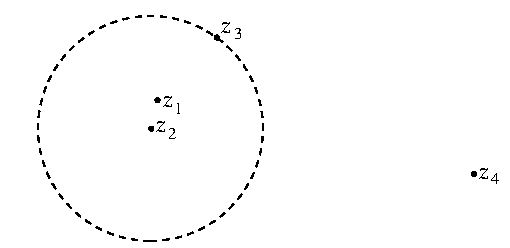
\includegraphics[width=0.8\linewidth]{figures/fig_2_1.pdf}
\caption{四つの局所演算子の積の期待値。OPE は、$z_1$ と $z_2$ の二つの演算子を $z_2$ の一つの演算子で置き換えた級数として、$z_1\to z_2$ での漸近的振る舞いを与える。収束半径は、最も近いほかの演算子までの距離であり、破線の円で示してある。}
\label{fig:2.1}
\end{figure}

ここでは、自由場の理論の特別な性質を用いて、$X^\mu$ 理論の OPE を導く。2.9節では、任意の共形不変な場の理論について導出する。

正規順序積が、素朴な運動方程式を満たすことを見た。式\hyperref[eq:2.1.23]{(2.1.23)}は、演算子積が $(z_1,\bar z_1)$ の調和関数であることを述べている。複素関数論の簡単な結果によれば、調和関数は局所的に、正則関数と反正則関数の和である。とくに、これは $z_1\to z_2$ で非特異であり、$z_{12}$ と $\bar z_{12}$ について自由に Taylor 展開できることを意味する。したがって、
\begin{equation}
\begin{aligned}
X^\mu(z_1,\bar z_1)X^\nu(z_2,\bar z_2)
={}&-\frac{\alpha'}2\eta^{\mu\nu}\ln|z_{12}|^2
+:X^\nu X^\mu(z_2,\bar z_2):\\
&+\sum_{k=1}^\infty\frac1{k!}\Bigl[
(z_{12})^k:X^\nu\partial^kX^\mu(z_2,\bar z_2):\\
&\hspace{8em}
+(\bar z_{12})^k:X^\nu\bar\partial^kX^\mu(z_2,\bar z_2):\Bigr].
\end{aligned}
\tag{2.2.4}\label{eq:2.2.4}
\end{equation}
混合した $\partial\bar\partial$ 微分を含む項は、運動方程式によって消える。この式とほかの多くの式は、$\alpha'=2$ とする単位で簡単になり、これが文献で最も一般的な規約である。しかし、ほかにもいくつかの規約が使われるため、$\alpha'$ を明示しておくと便利である。たとえば、開弦理論では $\alpha'=\tfrac12$ とすると式が簡単になる。

式\hyperref[eq:2.2.4]{(2.2.4)}は OPE の形をしている。その導出のもととなった運動方程式\hyperref[eq:2.1.23]{(2.1.23)}と同様に、これは演算子としての主張である。積 $X^\mu(z_1,\bar z_1)X^\nu(z_2,\bar z_2)$ に、ほかの点の場を掛けたものを含む任意の期待値に対して、$z_1\to z_2$ での振る舞いを無限級数として与える。各項は、$z_{12}$ および／または $\bar z_{12}$ の既知の関数と、二つの演算子を局所演算子で置き換えた期待値との積である。

OPE は通常、漸近展開として用いられ、最初の数項が小さい間隔での支配的な振る舞いを与える。本書の応用の大部分もこの種のものであり、しばしば OPE を、明示した特異項と、具体的に書かない非特異な残余との和として記す。「$=$」の代わりに「$\sim$」を用いたときは、「非特異な項を除いて等しい」という意味である。実際には、共形不変な場の理論では OPE は収束する。このことは、ある種の応用において非常に重要であり、係数関数から理論全体を再構成することを可能にする。一例として、自由場の OPE \hyperref[eq:2.2.4]{(2.2.4)}の任意の期待値における収束半径は、経路積分内の最も近いほかの挿入までの距離に等しい。演算子積は、演算子の位置を除いて調和関数であり、とくに図\hyperref[fig:2.1]{2.1}の破線の円の内部で調和である。そのため、複素関数論の標準的な議論によって収束を示すことができる。

OPE \hyperref[eq:2.2.4]{(2.2.4)}の右辺のさまざまな演算子には、同じ点における場の積が含まれている。場の量子論では、通常このような積は発散し、適切にカットオフを入れて繰り込まねばならないが、ここでは正規順序によって明確に定義される。正規順序は、自由場の理論で複合演算子を定義する便利な方法である。相互作用する場の理論の大部分では、相互作用頂点が複合演算子に近づいたり、互いに近づいたりすることによる追加の発散があるため、ほとんど役に立たない。しかし、われわれが関心をもつ場の理論の多くは自由であり、ほかの多くも自由場の理論と関係づけられる。したがって、正規順序をもう少し展開しておく価値がある。

任意の数の場に対する正規順序の定義は、次のように再帰的に与えられる。
\begin{equation}
\begin{aligned}
&:X^{\mu_1}(z_1,\bar z_1)\cdots X^{\mu_n}(z_n,\bar z_n):\\
&\qquad=X^{\mu_1}(z_1,\bar z_1)\cdots X^{\mu_n}(z_n,\bar z_n)
+\sum\text{減算項}.
\end{aligned}
\tag{2.2.5}\label{eq:2.2.5}
\end{equation}
ここで和は、積から一組、二組、あるいはそれ以上の場の対を選ぶすべての方法にわたり、それぞれの対を $\tfrac12\alpha'\eta^{\mu_i\mu_j}\ln|z_{ij}|^2$ で置き換える。たとえば、
\begin{equation}
\begin{aligned}
&:X^{\mu_1}(z_1,\bar z_1)X^{\mu_2}(z_2,\bar z_2)X^{\mu_3}(z_3,\bar z_3):\\
&\quad=X^{\mu_1}(z_1,\bar z_1)X^{\mu_2}(z_2,\bar z_2)X^{\mu_3}(z_3,\bar z_3)\\
&\qquad+\left(\frac{\alpha'}2\eta^{\mu_1\mu_2}\ln|z_{12}|^2
X^{\mu_3}(z_3,\bar z_3)+\text{二つの置換項}\right).
\end{aligned}
\tag{2.2.6}\label{eq:2.2.6}
\end{equation}
定義\hyperref[eq:2.2.5]{(2.2.5)}が、正規順序積は素朴な運動方程式を満たすという望ましい性質を保つことの証明は、読者に委ねる。

この定義は簡潔に
\begin{equation}
:\mathcal F:
=\exp\left(\frac{\alpha'}4\int d^2z_1d^2z_2\,
\ln|z_{12}|^2\,
\frac{\delta}{\delta X^\mu(z_1,\bar z_1)}
\frac{\delta}{\delta X_\mu(z_2,\bar z_2)}\right)\mathcal F
\tag{2.2.7}\label{eq:2.2.7}
\end{equation}
とまとめられる。ここで $\mathcal F$ は $X$ の任意の汎関数である。これは式\hyperref[eq:2.2.5]{(2.2.5)}と等価である。指数の中の二重微分が場の各対を縮約し、指数関数が任意の数の対について和をとる。その際、階乗が微分の作用の仕方の数を打ち消す。この形式的な表式の使い方の一例として、両辺に逆の指数関数を作用させると、
\begin{equation}
\begin{aligned}
\mathcal F
&=\exp\left(-\frac{\alpha'}4\int d^2z_1d^2z_2\,
\ln|z_{12}|^2\,
\frac{\delta}{\delta X^\mu(z_1,\bar z_1)}
\frac{\delta}{\delta X_\mu(z_2,\bar z_2)}\right):\mathcal F:\\
&=:\mathcal F:+\sum\text{縮約項}
\end{aligned}
\tag{2.2.8}\label{eq:2.2.8}
\end{equation}
を得る。ここで縮約は減算の逆であり、$:\mathcal F:$ から一組、二組、あるいはそれ以上の場の対を選ぶすべての方法について和をとり、各対を $-\tfrac12\alpha'\eta^{\mu_i\mu_j}\ln|z_{ij}|^2$ で置き換える。

任意の二つの演算子の OPE は、$X$ の任意の汎関数 $\mathcal F,\mathcal G$ に対する
\begin{equation}
:\mathcal F:\,:\mathcal G:
=:\mathcal F\mathcal G:+\sum\text{交差縮約項}
\tag{2.2.9}\label{eq:2.2.9}
\end{equation}
から生成できる。今度の和は、$\mathcal F$ 中の一つの場と $\mathcal G$ 中の一つの場を対にして縮約するすべての方法にわたる。これはまた、
\begin{equation}
:\mathcal F:\,:\mathcal G:
=\exp\left(-\frac{\alpha'}2\int d^2z_1d^2z_2\,\ln|z_{12}|^2\,
\frac{\delta}{\delta X_{\mathcal F}^{\mu}(z_1,\bar z_1)}
\frac{\delta}{\delta X_{\mathcal G\mu}(z_2,\bar z_2)}\right)
:\mathcal F\mathcal G:
\tag{2.2.10}\label{eq:2.2.10}
\end{equation}
とも書ける。ここで汎関数微分は、それぞれ $\mathcal F$ または $\mathcal G$ 中の場にだけ作用する。これは式\hyperref[eq:2.2.7]{(2.2.7)}から容易に従う。

一例として、
\begin{equation}
\begin{aligned}
&:\partial X^\mu(z)\partial X_\mu(z):
:\partial'X^\nu(z')\partial'X_\nu(z'):\\
&\quad=:\partial X^\mu(z)\partial X_\mu(z)
\partial'X^\nu(z')\partial'X_\nu(z'):\\
&\qquad-4\cdot\frac{\alpha'}2
\bigl(\partial\partial'\ln|z-z'|^2\bigr)
:\partial X^\mu(z)\partial'X_\mu(z'):\\
&\qquad+2\cdot\eta^\mu{}_\mu
\left(-\frac{\alpha'}2\partial\partial'\ln|z-z'|^2\right)^2\\
&\quad\sim\frac{D\alpha'^2}{2(z-z')^4}
-\frac{2\alpha'}{(z-z')^2}:\partial'X^\mu(z')\partial'X_\mu(z'):\\
&\qquad-\frac{2\alpha'}{z-z'}
:\partial'^2X^\mu(z')\partial'X_\mu(z'):.
\end{aligned}
\tag{2.2.11}\label{eq:2.2.11}
\end{equation}
等号の右辺の第2項は、一組の対を作る四つの方法から生じ、第3項は、二組の対を作る二つの方法から生じる。最後の式では、正規順序の内部で Taylor 展開してすべてを $z'$ の局所演算子で表し、最も特異な項を先頭に置くことで、OPE を標準形にしている。

もう一つの重要な例は
\begin{equation}
\mathcal F=e^{ik_1\cdot X(z,\bar z)},\qquad
\mathcal G=e^{ik_2\cdot X(0,0)}
\tag{2.2.12}\label{eq:2.2.12}
\end{equation}
である。変分 $\delta/\delta X_{\mathcal F}^\mu$ と
$\delta/\delta X_{\mathcal G}^\mu$ は、それぞれ $ik_{1\mu}$ と $ik_{2\mu}$ の因子を与える。したがって、一般的な結果\hyperref[eq:2.2.10]{(2.2.10)}は
\begin{equation}
\begin{aligned}
:e^{ik_1\cdot X(z,\bar z)}:\,:e^{ik_2\cdot X(0,0)}:
&=\exp\left(\frac{\alpha'}2k_1\cdot k_2\ln|z|^2\right)
:e^{ik_1\cdot X(z,\bar z)}e^{ik_2\cdot X(0,0)}:\\
&=|z|^{\alpha'k_1\cdot k_2}
:e^{ik_1\cdot X(z,\bar z)}e^{ik_2\cdot X(0,0)}:
\end{aligned}
\tag{2.2.13}\label{eq:2.2.13}
\end{equation}
となる。OPE を導くには、正規順序の内部で Taylor 展開して、
\begin{equation}
:e^{ik_1\cdot X(z,\bar z)}:\,:e^{ik_2\cdot X(0,0)}:
=|z|^{\alpha'k_1\cdot k_2}
:e^{i(k_1+k_2)\cdot X(0,0)}[1+O(z,\bar z)]:
\tag{2.2.14}\label{eq:2.2.14}
\end{equation}
を得ればよい。演習では、正規順序と自由場の OPE をさらに練習する。

OPE \hyperref[eq:2.2.2]{(2.2.2)}、\hyperref[eq:2.2.4]{(2.2.4)}などは、後者の点の周りで展開することで、$\sigma_1,\sigma_2$ に関して非対称に書かれていることに注意しよう。右辺を $(\sigma_1+\sigma_2)/2$ の周りで Taylor 展開すれば、対称な形にもできる。対称な形の係数関数は、二つの演算子の交換に対して単純に振る舞う。
\begin{equation}
c^k{}_{ij}(\sigma_1-\sigma_2)_{\mathrm{sym}}
=\pm c^k{}_{ji}(\sigma_2-\sigma_1)_{\mathrm{sym}}.
\tag{2.2.15}\label{eq:2.2.15}
\end{equation}
ここで、$\mathcal A_i$ と $\mathcal A_j$ がともに反交換する場合には、負号が現れる。計算には通常、非対称な形の方が便利であるため、係数関数の対称性が必要な場合には、対称な形でそれを求めてから、非対称な形に変換すればよい。

\subsectionlink{Ward 恒等式と Noether の定理}\label{sec:2.3}

世界面の対称性が弦理論で重要な役割を果たすことは、もちろんである。この節ではまず、場の理論における対称性の一般的な帰結をいくつか導く。

$d$ 次元時空における、作用 $S[\phi]$ をもつ一般の場の理論を考える。$\phi_\alpha(\sigma)$ は一般の場を表す。対称変換
\begin{equation}
\phi'_\alpha(\sigma)=\phi_\alpha(\sigma)+\delta\phi_\alpha(\sigma)
\tag{2.3.1}\label{eq:2.3.1}
\end{equation}
があり、$\delta\phi_\alpha$ は無限小パラメータ $\epsilon$ に比例するものとする。経路積分の測度と重み $\exp(-S)$ の積は不変である。
\begin{equation}
[d\phi']\exp\bigl(-S[\phi']\bigr)
=[d\phi]\exp\bigl(-S[\phi]\bigr).
\tag{2.3.2}\label{eq:2.3.2}
\end{equation}

場の理論の連続対称性は、保存カレントの存在（Noether の定理）と、カレントの演算子積を制約する Ward 恒等式を意味する。これらの結果を導くため、変数変換
\begin{equation}
\phi'_\alpha(\sigma)=\phi_\alpha(\sigma)
+\rho(\sigma)\delta\phi_\alpha(\sigma)
\tag{2.3.3}\label{eq:2.3.3}
\end{equation}
を考える。任意関数 $\rho(\sigma)$ を含めることで変換則を変更しているので、これは対称変換ではない。もし $\rho$ が定数なら、経路積分測度と $\exp(-S)$ の積は不変であるため、その変分は勾配 $\partial_a\rho$ に比例しなければならない。
\begin{equation}
\begin{aligned}
&[d\phi']\exp\bigl(-S[\phi']\bigr)\\
&\quad=[d\phi]\exp\bigl(-S[\phi]\bigr)
\left[1+\frac{i\epsilon}{2\pi}\int d^d\sigma\,g^{1/2}
j^a(\sigma)\partial_a\rho(\sigma)+O(\epsilon^2)\right].
\end{aligned}
\tag{2.3.4}\label{eq:2.3.4}
\end{equation}
未知の係数 $j^a(\sigma)$ は測度と作用の変分から生じ、それらはともに局所的である。したがって、これは場とその微分の局所関数でなければならない。関数 $\rho$ は小さな領域の内部だけでゼロでないとし、この領域の外に一般的な挿入「$\cdots$」をもつ経路積分を考える。すると、挿入は\hyperref[eq:2.3.3]{(2.3.3)}の下で不変である。変数変換に対する経路積分の不変性から、
\begin{equation}
\begin{aligned}
0&=\int[d\phi']\exp\bigl(-S[\phi']\bigr)\cdots
-\int[d\phi]\exp\bigl(-S[\phi]\bigr)\cdots\\
&=\frac{\epsilon}{2\pi i}\int d^d\sigma\,g^{1/2}\rho(\sigma)
\left\langle\nabla_aj^a(\sigma)\cdots\right\rangle
\end{aligned}
\tag{2.3.5}\label{eq:2.3.5}
\end{equation}
が得られる。$\rho$ の台が限られているため、部分積分を行うことができた。したがって、演算子方程式として
\begin{equation}
\nabla_aj^a=0
\tag{2.3.6}\label{eq:2.3.6}
\end{equation}
を得る。これが Noether の定理であり、演習2.5でさらに展開する。

Ward 恒等式を導くため、$\rho(\sigma)$ は、ある領域 $R$ の内部で1、外部で0とする。また、経路積分には、$R$ 内部の点 $\sigma_0$ に一般の局所演算子 $\mathcal A(\sigma_0)$ を含め、外部には通常どおり任意の挿入「$\cdots$」を含める。先ほどと同様に進めると、演算子関係
\begin{equation}
\delta\mathcal A(\sigma_0)
+\frac{\epsilon}{2\pi i}\int_Rd^d\sigma\,g^{1/2}
\nabla_aj^a(\sigma)\mathcal A(\sigma_0)=0
\tag{2.3.7}\label{eq:2.3.7}
\end{equation}
を得る。等価的に、
\begin{equation}
\nabla_aj^a(\sigma)\mathcal A(\sigma_0)
=g^{-1/2}\delta^d(\sigma-\sigma_0)\frac{2\pi}{i\epsilon}
\delta\mathcal A(\sigma_0)+\text{$\sigma$ に関する全微分}.
\tag{2.3.8}\label{eq:2.3.8}
\end{equation}
発散定理を用いると、
\begin{equation}
\int_{\partial R}dA\,n_aj^a\mathcal A(\sigma_0)
=\frac{2\pi}{i\epsilon}\delta\mathcal A(\sigma_0)
\tag{2.3.9}\label{eq:2.3.9}
\end{equation}
となる。ここで $dA$ は面積要素、$n^a$ は外向き法線である。これは、演算子の周囲でのカレントの積分を、その演算子の変分に関係づける。平坦な二次元に移ると、
\begin{equation}
\oint_{\partial R}(j\,dz-\tilde{\jmath}\,d\bar z)\mathcal A(z_0,\bar z_0)
=\frac{2\pi}{\epsilon}\delta\mathcal A(z_0,\bar z_0)
\tag{2.3.10}\label{eq:2.3.10}
\end{equation}
となる。ここでも添字を省き、$j\equiv j_z$、$\tilde{\jmath}\equiv j_{\bar z}$ としている。カレントでは、省略した添字は暗黙のうちに下付きであることに注意しよう。$\tilde{\jmath}$ に上線でなくチルダを用いるのは、これが $j$ の随伴ではないからである。Minkowski の密度 $j_0$ は一般に Hermite 的なので、余分な因子 $i$ をもつ Euclid の $j_2$ は反 Hermite 的であり、
$(j_z)^\dagger=\tfrac12(j_1-ij_2)^\dagger=j_z$ となる。

Noether の定理と Ward 恒等式が局所的な性質であることは重要である。これらは、遠く離れたところでどのような境界条件を課すかには依存せず、その境界条件が対称変換の下で不変かどうかにさえ依存しない。とくに、関数 $\rho(\sigma)$ は $R$ の内部だけでゼロでないので、対称変換はその内部で定義されていれば十分である。

共形不変な理論では通常、$j_z$ は正則であり、$j_{\bar z}$ は反正則である（ほかの場の位置での特異点を除く）。この場合、カレント $(j_z,0)$ と $(0,j_{\bar z})$ は別々に保存する。すると積分\hyperref[eq:2.3.10]{(2.3.10)}は、OPE の留数を取り出す。
\begin{equation}
\begin{aligned}
&\operatorname{Res}_{z\to z_0}j(z)\mathcal A(z_0,\bar z_0)
+\overline{\operatorname{Res}}_{\bar z\to\bar z_0}
\tilde{\jmath}(\bar z)\mathcal A(z_0,\bar z_0)\\
&\hspace{4em}=\frac{1}{i\epsilon}\delta\mathcal A(z_0,\bar z_0).
\end{aligned}
\tag{2.3.11}\label{eq:2.3.11}
\end{equation}
ここで「$\operatorname{Res}$」と「$\overline{\operatorname{Res}}$」は、それぞれ $(z-z_0)^{-1}$ と $(\bar z-\bar z_0)^{-1}$ の係数である。Ward 恒等式のこの形は、とくに便利である。世界面のカレントの定義に、場の理論における通常の定義に対して余分な因子 $2\pi i$ を入れたのは、この OPE を簡単にするためであった。

一例として、質量のない自由スカラーに戻り、時空の並進 $\delta X^\mu=\epsilon a^\mu$ を考える。$\delta X^\mu(\sigma)=\epsilon\rho(\sigma)a^\mu$ の下で、
\begin{equation}
\delta S=\frac{\epsilon a_\mu}{2\pi\alpha'}
\int d^2\sigma\,\partial^aX^\mu\partial_a\rho.
\tag{2.3.12}\label{eq:2.3.12}
\end{equation}
これは、述べた形\hyperref[eq:2.3.5]{(2.3.5)}をしており、Noether カレントは $a_\mu j_a^\mu$ である。ただし、
\begin{equation}
j_a^\mu=\frac{i}{\alpha'}\partial_aX^\mu.
\tag{2.3.13}\label{eq:2.3.13}
\end{equation}
各成分は、予想どおり正則および反正則である。このカレントと指数関数演算子の OPE は、一回の縮約を含む項から、
\begin{align}
j^\mu(z):e^{ik\cdot X(0,0)}:
&\sim\frac{k^\mu}{2z}:e^{ik\cdot X(0,0)}:,
\tag{2.3.14a}\label{eq:2.3.14a}\\
\tilde{\jmath}^\mu(\bar z):e^{ik\cdot X(0,0)}:
&\sim\frac{k^\mu}{2\bar z}:e^{ik\cdot X(0,0)}:
\tag{2.3.14b}\label{eq:2.3.14b}
\end{align}
と求まる。この OPE は、一般的な恒等式\hyperref[eq:2.3.11]{(2.3.11)}と一致している。

もう一つの例は、世界面の並進 $\delta\sigma^a=\epsilon v^a$ であり、その下で $\delta X^\mu=-\epsilon v^a\partial_aX^\mu$ となる。Noether カレントは
\begin{align}
j_a&=iv^bT_{ab},
\tag{2.3.15a}\label{eq:2.3.15a}\\
T_{ab}&=-\frac{1}{\alpha'}:
\left(\partial_aX^\mu\partial_bX_\mu
-\frac12\delta_{ab}\partial_cX^\mu\partial^cX_\mu\right):
\tag{2.3.15b}\label{eq:2.3.15b}
\end{align}
である。ここで $T_{ab}$ は世界面のエネルギー運動量テンソルである。\footnote[2]{$T_{ab}$ では、一点における演算子の積を定義するために正規順序を用いた。この繰り込みによって導入されうる曖昧さは、減算に由来する、定数倍の $\delta_{ab}$ だけである。そのような定数を加えると、やはり保存する別のエネルギー運動量テンソルが得られる。本書では、次章でより詳しく説明する理由により、テンソル\hyperref[eq:2.3.15b]{(2.3.15b)}に注目する。}

\subsectionlink{共形不変性}\label{sec:2.4}

エネルギー運動量テンソル\hyperref[eq:2.3.15b]{(2.3.15b)}はトレースがゼロである：$T^a{}_a=0$。複素座標では、これは
\begin{equation}
T_{z\bar z}=0
\tag{2.4.1}\label{eq:2.4.1}
\end{equation}
となる。すると、保存則 $\partial^aT_{ab}=0$ より、$T^a{}_a=0$ を満たす任意の理論で
\begin{equation}
\bar\partial T_{zz}=\partial T_{\bar z\bar z}=0
\tag{2.4.2}\label{eq:2.4.2}
\end{equation}
が従う。したがって、
\begin{equation}
T(z)\equiv T_{zz}(z),\qquad
\widetilde T(\bar z)\equiv T_{\bar z\bar z}(\bar z)
\tag{2.4.3}\label{eq:2.4.3}
\end{equation}
は、それぞれ正則および反正則である。質量のない自由スカラーでは、
\begin{equation}
T(z)=-\frac1{\alpha'}:\partial X^\mu\partial X_\mu:,\qquad
\widetilde T(\bar z)=-\frac1{\alpha'}:\bar\partial X^\mu\bar\partial X_\mu:
\tag{2.4.4}\label{eq:2.4.4}
\end{equation}
となり、運動方程式の帰結として、実際に正則および反正則である。

$T_{ab}$ のトレースがゼロであることは、はるかに大きな対称性を意味する。カレント
\begin{equation}
j(z)=iv(z)T(z),\qquad
\tilde{\jmath}(\bar z)=iv(z)^*\widetilde T(\bar z)
\tag{2.4.5}\label{eq:2.4.5}
\end{equation}
は、任意の正則関数 $v(z)$ に対して保存する。自由スカラー理論では、OPE
\begin{equation}
T(z)X^\mu(0)\sim\frac1z\partial X^\mu(0),\qquad
\widetilde T(\bar z)X^\mu(0)\sim\frac1{\bar z}\bar\partial X^\mu(0)
\tag{2.4.6}\label{eq:2.4.6}
\end{equation}
が得られる。すると Ward 恒等式は、変換
\begin{equation}
\delta X^\mu=-\epsilon v(z)\partial X^\mu
-\epsilon v(z)^*\bar\partial X^\mu
\tag{2.4.7}\label{eq:2.4.7}
\end{equation}
を与える。これは無限小座標変換 $z'=z+\epsilon v(z)$ である。有限変換は、任意の正則関数 $f(z)$ に対して、
\begin{equation}
X'^\mu(z',\bar z')=X^\mu(z,\bar z),\qquad z'=f(z)
\tag{2.4.8}\label{eq:2.4.8}
\end{equation}
である。これは共形変換と呼ばれる。

ここで見いだした共形対称性を、一般相対論の微分同相不変性と混同してはならない。ここで扱っているのは平坦な空間の理論であり、変化させる独立な計量場はないので、変換 $z\to z'$ は点の間の距離を実際に変える。このような不変性は普通は存在せず、これは力学に関する非自明な主張である。スカラーの作用\hyperref[eq:2.1.10]{(2.1.10)}では、$\partial,\bar\partial$ の共形変換が、ちょうど $d^2z$ の変換を相殺する。質量項 $m^2X^\mu X_\mu$ は不変ではないであろう。最終的には Polyakov 弦の $\text{diff}\times\text{Weyl}$ 対称性と密接な関係があることは明らかだが、それは次章に譲る。

複素数 $\zeta$ に対する特殊な場合
\begin{equation}
z'=\zeta z
\tag{2.4.9}\label{eq:2.4.9}
\end{equation}
を考えよう。$\zeta$ の位相は系の回転であり、その絶対値は系の大きさのスケール変換である。このようなスケール不変性は、素粒子物理で近似的な対称性としてときどき考えられてきた。また、臨界点にある統計系は、スケール不変な場の理論によって記述される。

一般の共形変換を理解するため、その無限小距離 $ds^2=d\sigma^a d\sigma^a=dz\,d\bar z$ への作用を考えよう。共形変換はこれを、位置に依存する因子でスケール変換する。
\begin{equation}
ds'^2=dz'\,d\bar z'
=\frac{\partial z'}{\partial z}\frac{\partial\bar z'}{\partial\bar z}
dz\,d\bar z.
\tag{2.4.10}\label{eq:2.4.10}
\end{equation}
したがって、図\hyperref[fig:2.2]{2.2}に示すように、共形変換は無限小の正方形を無限小の正方形へ移すが、その大きさを位置に依存する因子で変える。反正則関数 $z'=f(z)^*$ も同じ性質をもつが、向きを変える。一様なスケール変換\hyperref[eq:2.4.9]{(2.4.9)}で不変な系の大部分は、実際には、それよりはるかに大きな共形対称性の下で不変である。この不変性をもつ理論を共形場理論（CFT）という。二次元を超える次元での共形不変性は、演習2.6で展開する。

\begin{figure}[htbp]
\centering
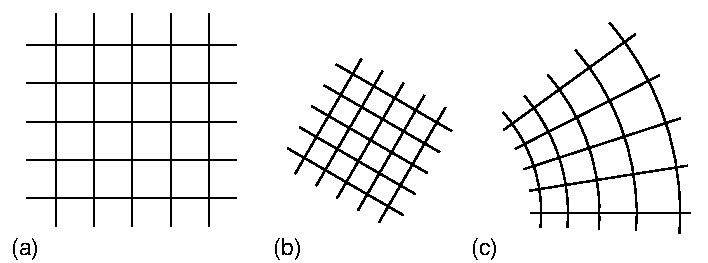
\includegraphics[width=0.8\linewidth]{figures/fig_2_2.pdf}
\caption{(a) 二次元の領域。(b) 特殊な共形変換\hyperref[eq:2.4.9]{(2.4.9)}の作用。(c) より一般的な共形変換の作用。}
\label{fig:2.2}
\end{figure}

\subsubsection*{共形不変性と OPE}

共形不変性は OPE の形、とくにエネルギー運動量テンソルの OPE に強い制約を課す。$T$ と一般の演算子 $\mathcal A$ の OPE を考えよう。$T(z)$ と $\widetilde T(\bar z)$ は挿入の位置を除いて（反）正則なので、対応する係数関数もこの性質をもたなければならない。したがって、$T$ と一般の $\mathcal A$ の OPE は、$z$ の整数べきで、ただし負のべきを含みうる Laurent 展開となる。さらに、すべての特異項は $\mathcal A$ の共形変換によって決まる。これを見るため、特異項の一般的な展開を
\begin{equation}
T(z)\mathcal A(0,0)\sim
\sum_{n=0}^{\infty}\frac1{z^{n+1}}\mathcal A^{(n)}(0,0)
\tag{2.4.11}\label{eq:2.4.11}
\end{equation}
と書き、$\widetilde T$ についても同様に書こう。演算子係数 $\mathcal A^{(n)}$ は、まだ決まっていない。無限小共形変換 $z'=z+\epsilon v(z)$ の下では、$T\mathcal A$ の OPE の $z^{-n-1}$ の項と $v(z)$ の $z^n$ 次の項を掛けたとき、$v(z)T(z)\mathcal A(0,0)$ に単純極が生じる。したがって、\hyperref[eq:2.3.11]{(2.3.11)}の形の Ward 恒等式は、
\begin{equation}
\delta\mathcal A(z,\bar z)
=-\epsilon\sum_{n=0}^\infty\frac1{n!}
\left[\partial^nv(z)\mathcal A^{(n)}(z,\bar z)
+\bar\partial^nv(z)^*\widetilde{\mathcal A}^{(n)}(z,\bar z)\right]
\tag{2.4.12}\label{eq:2.4.12}
\end{equation}
を意味する。よって、演算子 $\mathcal A^{(n)}$ は $\mathcal A$ の共形変換によって決まる。

局所演算子の基底には、一様な変換\hyperref[eq:2.4.9]{(2.4.9)}の下で固有状態となるものをとると便利である。
\begin{equation}
\mathcal A'(z',\bar z')=\zeta^{-h}\bar\zeta^{-\tilde h}\mathcal A(z,\bar z).
\tag{2.4.13}\label{eq:2.4.13}
\end{equation}
$(h,\tilde h)$ は $\mathcal A$ のウェイトと呼ばれる。和 $h+\tilde h$ は $\mathcal A$ の次元であり、スケール変換の下での振る舞いを決める。一方、$h-\tilde h$ はスピンであり、回転の下での振る舞いを決める。微分 $\partial_z$ は $h$ を一つ増やし、微分 $\partial_{\bar z}$ は $\tilde h$ を一つ増やす。変換\hyperref[eq:2.4.13]{(2.4.13)}および並進
$\delta\mathcal A=-\epsilon v^a\partial_a\mathcal A$ に対する Ward 恒等式は、OPE の一部を決める。
\begin{equation}
T(z)\mathcal A(0,0)
=\cdots+\frac h{z^2}\mathcal A(0,0)
+\frac1z\partial\mathcal A(0,0)+\cdots.
\tag{2.4.14}\label{eq:2.4.14}
\end{equation}
$\widetilde T$ についても同様である。

重要な特殊例は、テンソル演算子、あるいは一次場\footnote[3]{場の量子論では通常、基本場（経路積分での積分変数）と、複合的でありうる、より一般的な演算子を区別する。実際には、この区別は主として三次元以上の弱結合の場の理論で有用である。CFT では、とくに異なる場の理論の間に等価関係があるため、ほとんど役に立たない。そこで、任意の局所演算子に対して「場」という語を用いる。}
$\mathcal O$ であり、一般の共形変換はそれに
\begin{equation}
\mathcal O'(z',\bar z')
=(\partial_z z')^{-h}
(\partial_{\bar z}\bar z')^{-\tilde h}\mathcal O(z,\bar z)
\tag{2.4.15}\label{eq:2.4.15}
\end{equation}
と作用する。OPE \hyperref[eq:2.4.11]{(2.4.11)}は
\begin{equation}
T(z)\mathcal O(0,0)
=\frac h{z^2}\mathcal O(0,0)+\frac1z\partial\mathcal O(0,0)+\cdots
\tag{2.4.16}\label{eq:2.4.16}
\end{equation}
に帰着し、一般の OPE \hyperref[eq:2.4.14]{(2.4.14)}にある、より特異な項は存在しない。

再び自由な $X^\mu$ の CFT を例にとると、いくつかの代表的な演算子のウェイトは
\begin{equation}
\left.
\begin{array}{c@{\quad}c@{\qquad}c@{\quad}c}
X^\mu&(0,0)&\partial X^\mu&(1,0)\\
\bar\partial X^\mu&(0,1)&\partial^2X^\mu&(2,0)\\
:e^{ik\cdot X}:&
\displaystyle\left(\frac{\alpha'k^2}4,\frac{\alpha'k^2}4\right)&&
\end{array}
\right\}
\tag{2.4.17}\label{eq:2.4.17}
\end{equation}
である。$\partial^2X^\mu$ を除き、すべてテンソルとして変換する。より一般に、指数関数と微分の一般的な積を掛けたもの
\begin{equation}
:\left(\prod_i\partial^{m_i}X^{\mu_i}\right)
\left(\prod_j\bar\partial^{n_j}X^{\nu_j}\right)e^{ik\cdot X}:
\tag{2.4.18}\label{eq:2.4.18}
\end{equation}
のウェイトは
\begin{equation}
\left(\frac{\alpha'k^2}4+\sum_i m_i,\,
\frac{\alpha'k^2}4+\sum_j n_j\right)
\tag{2.4.19}\label{eq:2.4.19}
\end{equation}
である。

任意の二つの演算子について、一様な並進、スケール変換、回転を OPE の両辺に適用すると、係数関数の $z$ 依存性が完全に決まる。
\begin{equation}
\mathcal A_i(z_1,\bar z_1)\mathcal A_j(z_2,\bar z_2)
=\sum_k z_{12}^{h_k-h_i-h_j}
\bar z_{12}^{\tilde h_k-\tilde h_i-\tilde h_j}
c^k{}_{ij}\mathcal A_k(z_2,\bar z_2).
\tag{2.4.20}\label{eq:2.4.20}
\end{equation}
ここでは、$c^k{}_{ij}$ は定数となっている。関心のあるすべての場合において、OPE \hyperref[eq:2.4.20]{(2.4.20)}の右辺に現れるウェイトは下から有界であるため、演算子積の特異性の次数は有界である。より一般的な共形変換は OPE にさらに制約を課す。それらは、すべての場の OPE を、一次場の OPE によって決定する。このことは第15章で展開する。

正規順序積の共形変換の性質は、一般には、その積の素朴な変換では与えられないことに注意しよう。たとえば、$X^\mu$ の変換則\hyperref[eq:2.4.7]{(2.4.7)}は、指数関数に対して、素朴には
\begin{equation}
\delta e^{ik\cdot X}
=-\epsilon v(z)\partial e^{ik\cdot X}
-\epsilon v(z)^*\bar\partial e^{ik\cdot X}
\qquad\text{（素朴な式）}
\tag{2.4.21}\label{eq:2.4.21}
\end{equation}
を意味し、それをウェイト $(0,0)$ のテンソルにするはずである。この修正は量子効果であり、一点における演算子の積を定義するために必要な繰り込みによる。具体的には、ここでは正規順序記号 $:\ :$ に含まれる減算 $\ln|z_{12}|^2$ が、座標系を明示的に参照しているために現れる。

\subsubsection*{エネルギー運動量テンソルの共形的性質}

エネルギー運動量テンソルとそれ自身の OPE は、式\hyperref[eq:2.2.11]{(2.2.11)}で得られている。
\begin{equation}
\begin{aligned}
T(z)T(0)
&=\frac{\eta^\mu{}_\mu}{2z^4}
-\frac2{\alpha' z^2}:\partial X^\mu(z)\partial X_\mu(0):
+:T(z)T(0):\\
&\sim\frac D{2z^4}+\frac2{z^2}T(0)+\frac1z\partial T(0).
\end{aligned}
\tag{2.4.22}\label{eq:2.4.22}
\end{equation}
$\widetilde T$ についても同様の結果が成り立つ。$T(z)\widetilde T(\bar z')$ の OPE は非特異でなければならない。点が離れているときには $z'$ に関して反正則なので、$(z-z')$ の極はもてない。同様に、点が離れているときには $z$ に関して正則なので、$(\bar z-\bar z')$ の極ももてない。\footnote[4]{特に断らない限り、OPE は点の間隔がゼロでない場合にのみ成り立ち、デルタ関数の可能性は無視している。本書での応用では、後者は問題にならない。デルタ関数を含めることが有用な場合もあるが、一般にその一部は定義に依存するので、注意が必要である。}
正則演算子と反正則演算子の間の任意の OPE についても、同じことが成り立つ。

したがって、$T$ はテンソルではない。OPE \hyperref[eq:2.4.22]{(2.4.22)}が意味する変換則は、
\begin{equation}
\epsilon^{-1}\delta T(z)
=-\frac D{12}\partial_z^3v(z)
-2\partial_zv(z)T(z)-v(z)\partial_zT(z)
\tag{2.4.23}\label{eq:2.4.23}
\end{equation}
である。

一般の CFT では、$T(z)$ は
\begin{equation}
\epsilon^{-1}\delta T(z)
=-\frac c{12}\partial_z^3v(z)
-2\partial_zv(z)T(z)-v(z)\partial_zT(z)
\tag{2.4.24}\label{eq:2.4.24}
\end{equation}
と変換する。$c$ は中心電荷と呼ばれる定数である。一つの自由スカラーの中心電荷は1であり、$D$ 個の自由スカラーでは $D$ である。変換\hyperref[eq:2.4.24]{(2.4.24)}は、$v$ に関して線形で、$TT$ の OPE の対称性と整合し、一様なスケール変換と回転に対する不変性が要求する三つの下付き $z$ 添字をもつ、最も一般的な形である。スケール変換、回転、並進の対称性は、第2項と第3項の係数を決める。さらに、このような二つの変換の交換子を考えると、$\partial_ac=0$ を示すことができる。そして、位置に依存しない演算子は $c$ 数でなければならないというのは、場の量子論の一般的な結果である。\footnote[5]{議論は次のとおりである。$\mathcal A(\sigma)$ は位置に依存しないと仮定し、ほかの任意の局所演算子 $\mathcal B(\sigma')$ との等時刻交換子を考える。局所性により、空間的に離れていれば両者は可換である。$\mathcal A(\sigma)$ は実際には位置に依存しないので、間隔がゼロでも可換である。したがって、$\mathcal A(\sigma)$ はすべての局所演算子と可換であり、$c$ 数でなければならない。}
対応する $TT$ の OPE は
\begin{equation}
T(z)T(0)\sim\frac c{2z^4}+\frac2{z^2}T(0)+\frac1z\partial T(0)
\tag{2.4.25}\label{eq:2.4.25}
\end{equation}
である。変換則\hyperref[eq:2.4.24]{(2.4.24)}の有限の形は
\begin{equation}
(\partial_z z')^2T'(z')=T(z)-\frac c{12}\{z',z\}
\tag{2.4.26}\label{eq:2.4.26}
\end{equation}
である。ここで $\{f,z\}$ は Schwarz 微分
\begin{equation}
\{f,z\}=\frac{2\partial_z^3f\,\partial_zf
-3\partial_z^2f\,\partial_z^2f}
{2\partial_zf\,\partial_zf}
\tag{2.4.27}\label{eq:2.4.27}
\end{equation}
を表す。これは、無限小の形が正しいこと、そして相次ぐ変換の下で正しく合成されることを確認すれば検証できる（したがって、無限小変換を積分できる）。$\widetilde T$ にも対応する形が成り立つが、一般の CFT では、異なる中心電荷 $\tilde c$ をもつ可能性がある。

後で見るように、エネルギー運動量テンソルがテンソルとして振る舞わないことは、いくつかの重要な物理的帰結をもつ。「テンソルでない」とは、共形変換について述べていることを強調しておく。エネルギー運動量テンソルは、座標変換の下では通常のテンソルとしての性質をもつ。

\subsectionlink{自由な共形場理論}\label{sec:2.5}

この節では、自由場の CFT の三つの族、すなわち線形ディラトン理論、$bc$ 理論、$\beta\gamma$ 理論を論じる。$bc$ 理論は、次章で Polyakov 弦のゲージを固定するときに現れるので、最も直接的に関心のあるものである。しかし、いずれも弦理論にさまざまな応用をもつ。

\subsubsection*{線形ディラトン CFT}

この CFT の族は、同じ作用\hyperref[eq:2.1.10]{(2.1.10)}に基づくが、エネルギー運動量テンソルは
\begin{align}
T(z)&=-\frac1{\alpha'}:\partial X^\mu\partial X_\mu:
+V_\mu\partial^2X^\mu,
\tag{2.5.1a}\label{eq:2.5.1a}\\
\widetilde T(\bar z)&=-\frac1{\alpha'}:\bar\partial X^\mu\bar\partial X_\mu:
+V_\mu\bar\partial^2X^\mu
\tag{2.5.1b}\label{eq:2.5.1b}
\end{align}
である。ここで $V_\mu$ は、ある固定された $D$ 元ベクトルである。$TT$ の OPE を計算すると、標準形\hyperref[eq:2.4.25]{(2.4.25)}であることがわかるが、その中心電荷は
\begin{equation}
c=\tilde c=D+6\alpha' V_\mu V^\mu
\tag{2.5.2}\label{eq:2.5.2}
\end{equation}
となる。$TX^\mu$ の OPE と Ward 恒等式\hyperref[eq:2.4.12]{(2.4.12)}は、共形変換
\begin{equation}
\delta X^\mu=-\epsilon v\partial X^\mu
-\epsilon v^*\bar\partial X^\mu
-\frac\epsilon2\alpha' V^\mu\left[\partial v+(\partial v)^*\right]
\tag{2.5.3}\label{eq:2.5.3}
\end{equation}
を意味する。これは、同じ作用の異なる共形対称性である。場 $X^\mu$ はもはやテンソルとしては変換せず、その変分は非斉次な部分をもつ。ちなみに、二次元の質量のない自由スカラーは、驚くほど多くの対称性をもっており、本書で言及する機会のあるものよりもはるかに多い。

エネルギー運動量テンソルは弦理論で特別な役割を果たし、とくに曲がった計量との結合の仕方を教える。したがって、異なる $V^\mu$ の値は異なる CFT とみなすべきである。ベクトル $V^\mu$ は、時空内の一つの方向を選び出す。そのため、この CFT は Lorentz 不変ではなく、当面のわれわれの関心の対象ではない。この線形ディラトン CFT の物理的解釈の一つを3.7節で見て、後にはいくつかの技術的応用で出会うことになる。

自由スカラー CFT の別の変形は、$X^\mu$ のいくつかを周期的にすることである。これは第8章で取り上げる。

\subsubsection*{$bc$ CFT}

第二の CFT の族は、反交換する場 $b,c$ と作用
\begin{equation}
S=\frac1{2\pi}\int d^2z\,b\bar\partial c
\tag{2.5.4}\label{eq:2.5.4}
\end{equation}
をもつ。任意に与えられた定数 $\lambda$ に対して、
\begin{equation}
h_b=\lambda,\qquad h_c=1-\lambda
\tag{2.5.5}\label{eq:2.5.5}
\end{equation}
を満たすウェイト $(h_b,0)$ と $(h_c,0)$ のテンソルとして $b,c$ が変換するとき、これは共形不変である。したがって、別の CFT の族を得る（第10章で学ぶように、これは実は線形ディラトンの族と同じものである）。以前と同じ方法\hyperref[eq:2.1.15]{(2.1.15)}、\hyperref[eq:2.1.18]{(2.1.18)}で得られる演算子の運動方程式は
\begin{align}
\bar\partial c(z)&=\bar\partial b(z)=0,
\tag{2.5.6a}\label{eq:2.5.6a}\\
\bar\partial b(z)c(0)&=2\pi\delta^2(z,\bar z)
\tag{2.5.6b}\label{eq:2.5.6b}
\end{align}
である。$bb$ と $cc$ の OPE は、源のない運動方程式を満たす。正規順序化された $bc$ 積は
\begin{equation}
:b(z_1)c(z_2):=b(z_1)c(z_2)-\frac1{z_{12}}
\tag{2.5.7}\label{eq:2.5.7}
\end{equation}
である。これは、
\begin{equation}
\bar\partial\frac1z=\partial\frac1{\bar z}
=2\pi\delta^2(z,\bar z)
\tag{2.5.8}\label{eq:2.5.8}
\end{equation}
の帰結として、素朴な運動方程式を満たす。この式は、原点を含む領域で積分し、微分を部分積分することで確認できる。場の一般の積の正規順序化は、組合せの面では $X^\mu$ の CFT と同じであり、縮約項または減算項についての和である。$b,c$ は反交換するため、場を交換すると符号が反転することに注意しなければならない。対にする場を、減算\hyperref[eq:2.5.7]{(2.5.7)}で置き換える前に、反交換させて隣り合う位置まで移すべきである。

演算子積は
\begin{equation}
b(z_1)c(z_2)\sim\frac1{z_{12}},\qquad
c(z_1)b(z_2)\sim\frac1{z_{12}}
\tag{2.5.9}\label{eq:2.5.9}
\end{equation}
である。第二の OPE では、反交換によるものと $z_1\leftrightarrow z_2$ によるものの、二つの符号反転が起こっている。ほかの演算子積は非特異である。
\begin{equation}
b(z_1)b(z_2)=O(z_{12}),\qquad
c(z_1)c(z_2)=O(z_{12}).
\tag{2.5.10}\label{eq:2.5.10}
\end{equation}
これらは正則であるだけでなく、反対称性のために零点をもつ。

Noether の定理から、エネルギー運動量テンソル
\begin{align}
T(z)&=:(\partial b)c:-\lambda\partial(:bc:),
\tag{2.5.11a}\label{eq:2.5.11a}\\
\widetilde T(\bar z)&=0
\tag{2.5.11b}\label{eq:2.5.11b}
\end{align}
が得られる。$T$ と $b,c$ の OPE を計算することによっても、\hyperref[eq:2.5.11a]{(2.5.11)}を確認できる。その OPE は、与えられたウェイトをもつ標準的なテンソルの形\hyperref[eq:2.4.16]{(2.4.16)}になる。$TT$ の OPE は標準形\hyperref[eq:2.4.25]{(2.4.25)}であり、
\begin{equation}
c=-3(2\lambda-1)^2+1,\qquad \tilde c=0
\tag{2.5.12}\label{eq:2.5.12}
\end{equation}
である。これは純粋に正則な CFT であり、$c\ne\tilde c$ となる例である。もちろん、対応する反正則な理論
\begin{equation}
S=\frac1{2\pi}\int d^2z\,\tilde b\,\partial\tilde c
\tag{2.5.13}\label{eq:2.5.13}
\end{equation}
もあり、これは上の理論で $z\leftrightarrow\bar z$ としたものと同じである。

$bc$ 理論は、ゴースト数の対称性 $\delta b=-i\epsilon b$、$\delta c=i\epsilon c$ をもつ。対応する Noether カレントは
\begin{equation}
j=-:bc:
\tag{2.5.14}\label{eq:2.5.14}
\end{equation}
である。ここでも成分は別々に正則と反正則であり、後者はゼロである。正則な $bc$ 場と反正則な $bc$ 場の両方がある場合には、それぞれのゴースト数が別々に保存する。

このカレントはテンソルではない。
\begin{equation}
T(z)j(0)\sim\frac{1-2\lambda}{z^3}
+\frac1{z^2}j(0)+\frac1z\partial j(0).
\tag{2.5.15}\label{eq:2.5.15}
\end{equation}
これは変換則
\begin{equation}
\epsilon^{-1}\delta j=-v\partial j-j\partial v
+\frac{2\lambda-1}{2}\partial^2v
\tag{2.5.16}\label{eq:2.5.16}
\end{equation}
を意味し、その有限の形は
\begin{equation}
(\partial_z z')j_{z'}(z')
=j_z(z)+\frac{2\lambda-1}{2}
\frac{\partial_z^2z'}{\partial_z z'}
\tag{2.5.17}\label{eq:2.5.17}
\end{equation}
である。

$b,c$ が等しいウェイトをもつ唯一の場合は $h_b=h_c=\tfrac12$ であり、このとき中心電荷は $c=1$ である。この場合には、$b\to\psi$、$c\to\bar\psi$ という記法をしばしば用いる。この場合、$bc$ CFT は共形不変性を保って二つに分割できる。
\begin{align}
\psi&=2^{-1/2}(\psi_1+i\psi_2),\qquad
\bar\psi=2^{-1/2}(\psi_1-i\psi_2),
\tag{2.5.18a}\label{eq:2.5.18a}\\
S&=\frac1{4\pi}\int d^2z\,
\left(\psi_1\bar\partial\psi_1+\psi_2\bar\partial\psi_2\right),
\tag{2.5.18b}\label{eq:2.5.18b}\\
T&=-\frac12\psi_1\partial\psi_1-\frac12\psi_2\partial\psi_2.
\tag{2.5.18c}\label{eq:2.5.18c}
\end{align}
各 $\psi$ 理論は、中心電荷 $\tfrac12$ をもつ。

$\lambda=2$、ウェイト $(h_b,h_c)=(2,-1)$ の $bc$ 理論は、次章で Polyakov 弦のゲージ固定に伴う Faddeev--Popov ゴーストとして現れる。$\psi$ 理論は、第2巻のより一般的な弦理論に広く現れる。

\subsubsection*{$\beta\gamma$ CFT}

第三の CFT の族は $bc$ 理論とよく似ているが、場は可換である。$\beta$ は $(h_\beta,0)$ テンソル、$\gamma$ は $(h_\gamma,0)$ テンソルであり、
\begin{equation}
h_\beta=\lambda,\qquad h_\gamma=1-\lambda
\tag{2.5.19}\label{eq:2.5.19}
\end{equation}
である。作用は
\begin{equation}
S=\frac1{2\pi}\int d^2z\,\beta\bar\partial\gamma
\tag{2.5.20}\label{eq:2.5.20}
\end{equation}
である。これらの場も、運動方程式
\begin{equation}
\bar\partial\gamma(z)=\bar\partial\beta(z)=0
\tag{2.5.21}\label{eq:2.5.21}
\end{equation}
によって正則となる。運動方程式と演算子積は、標準的な方法で導かれる。統計が変わっているため、演算子積の一部の符号は異なる。
\begin{equation}
\beta(z_1)\gamma(z_2)\sim-\frac1{z_{12}},\qquad
\gamma(z_1)\beta(z_2)\sim\frac1{z_{12}}.
\tag{2.5.22}\label{eq:2.5.22}
\end{equation}
エネルギー運動量テンソルは
\begin{align}
T&=:(\partial\beta)\gamma:-\lambda\partial(:\beta\gamma:),
\tag{2.5.23a}\label{eq:2.5.23a}\\
\widetilde T&=0
\tag{2.5.23b}\label{eq:2.5.23b}
\end{align}
である。中心電荷は、単に符号が逆になる。
\begin{equation}
c=3(2\lambda-1)^2-1,\qquad \tilde c=0.
\tag{2.5.24}\label{eq:2.5.24}
\end{equation}
$\lambda=\tfrac32$、ウェイト $(h_\beta,h_\gamma)=(\tfrac32,-\tfrac12)$ の $\beta\gamma$ 理論は、第10章で超弦のゲージ固定に伴う Faddeev--Popov ゴーストとして現れる。

\providecommand{\canorm}[1]{\mathopen{{}^{\circ}_{\circ}}#1\mathclose{{}^{\circ}_{\circ}}}
\subsectionlink{Virasoro 代数}
\label{sec:2.6}

この章ではここまで、2次元の場の理論の局所的な性質を調べてきた。ここからは理論のスペクトルに関心を移す。空間座標は閉弦の場合のように周期的であるか、開弦の場合のように有界であるものとする。

周期的な場合には、
\begin{equation}
\sigma^1\sim\sigma^1+2\pi.
\tag{2.6.1}\label{eq:2.6.1}
\end{equation}
Euclid 時間座標の範囲を
\begin{equation}
-\infty<\sigma^2<\infty
\tag{2.6.2}\label{eq:2.6.2}
\end{equation}
とし、2次元の領域が無限円筒をなすようにする。ここでも複素座標を作ると便利であり、自然な選択が二つある。第1は
\begin{equation}
w=\sigma^1+i\sigma^2,
\tag{2.6.3}\label{eq:2.6.3}
\end{equation}
であり、$w\sim w+2\pi$ となる。第2は
\begin{equation}
z=\exp(-iw)=\exp(-i\sigma^1+\sigma^2).
\tag{2.6.4}\label{eq:2.6.4}
\end{equation}
この二つの座標系を図\ref{fig:2.3}に示す。$w$ 座標では、時間は $\sigma^2=\operatorname{Im}w$ の並進に対応する。$z$ では時間は動径方向に進み、原点が無限の過去になる。これらの座標は共形変換で結ばれている。$w$ 座標は理論の正準的な解釈に自然だが、$z$ 座標もきわめて有用であり、ほとんどの式はこちらの座標系で書かれる。

\begin{figure}[htbp]
\centering
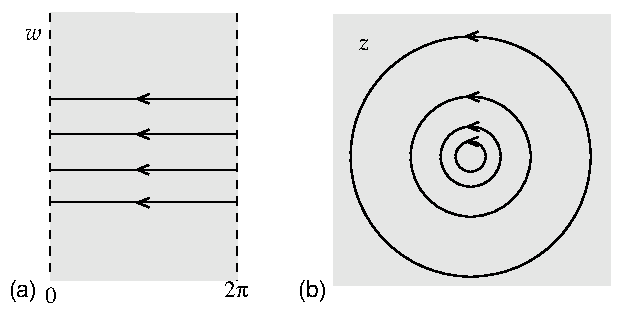
\includegraphics[width=0.8\linewidth]{figures/fig_2_3.pdf}
\caption{閉弦の座標。(a) $w$ 平面の等時刻積分路。破線同士は同一視する。(b) $z$ 平面での同じ積分路。}
\label{fig:2.3}
\end{figure}

正則または反正則な演算子には Laurent 展開が可能である：
\begin{equation}
T_{zz}(z)=\sum_{m=-\infty}^{\infty}\frac{L_m}{z^{m+2}},
\qquad
\widetilde T_{\bar z\bar z}(\bar z)
=\sum_{m=-\infty}^{\infty}\frac{\widetilde L_m}{\bar z^{m+2}}.
\tag{2.6.5}\label{eq:2.6.5}
\end{equation}
Virasoro 生成子として知られる Laurent 係数は、周回積分
\begin{equation}
L_m=\oint_C\frac{dz}{2\pi iz}\,z^{m+2}T_{zz}(z)
\tag{2.6.6}\label{eq:2.6.6}
\end{equation}
で与えられる。ここで $C$ は原点を反時計回りに囲む任意の積分路である。Laurent 展開は、時刻 $\sigma^2=0$ での $w$ 座標系における通常の Fourier 変換と同じである：
\begin{align}
T_{ww}(w)&=-\sum_{m=-\infty}^{\infty}
\exp(im\sigma^1-m\sigma^2)T_m,
\tag{2.6.7a}\label{eq:2.6.7a}\\
T_{\bar w\bar w}(\bar w)&=-\sum_{m=-\infty}^{\infty}
\exp(-im\sigma^1-m\sigma^2)\widetilde T_m,
\tag{2.6.7b}\label{eq:2.6.7b}
\end{align}
ここで
\begin{equation}
T_m=L_m-\delta_{m,0}\frac c{24},\qquad
\widetilde T_m=\widetilde L_m-\delta_{m,0}\frac{\widetilde c}{24}.
\tag{2.6.8}\label{eq:2.6.8}
\end{equation}
$T_0$ の加法的なずれは、テンソル的でない変換 \hyperref[eq:2.4.26]{(2.4.26)}、
\begin{equation}
T_{ww}=(\partial_w z)^2T_{zz}+\frac c{24}
\tag{2.6.9}\label{eq:2.6.9}
\end{equation}
から生じる。$w=\sigma^1+i\sigma^2$ 座標系で時間並進を生成する Hamiltonian $H$ は
\begin{equation}
H=\int_0^{2\pi}\frac{d\sigma^1}{2\pi}\,T_{22}
=L_0+\widetilde L_0-\frac{c+\widetilde c}{24}.
\tag{2.6.10}\label{eq:2.6.10}
\end{equation}
Laurent 展開 \hyperref[eq:2.6.5]{(2.6.5)} にある $+2$ は、$T$ の共形変換により Fourier 展開 \hyperref[eq:2.6.7a]{(2.6.7)} では相殺されていることに注意しよう。同様に、ウェイト $h$ の正則場の Laurent 展開では、指数に $+h$ が含まれる。

時刻 $\operatorname{Im}w=\ln|z|$ が一定の円で経路積分を切り開くと、Virasoro 生成子は通常の意味の演算子になる。（経路積分を切り開くという考え方は付録で展開する。）正則性により、積分 \hyperref[eq:2.6.6]{(2.6.6)} は $C$ に依存せず、とくに時間並進（動径方向のスケール変換）に対して不変である。すなわち、これらは保存電荷であり、共形変換に対応する電荷である。

カレントの OPE が、それに対応する電荷の代数を決めることは重要な事実である。正則カレントの周回積分として与えられる一般の電荷 $Q_i$、$i=1,2$ を考える：
\begin{equation}
Q_i\{C\}=\oint_C\frac{dz}{2\pi i}\,j_i.
\tag{2.6.11}\label{eq:2.6.11}
\end{equation}
組み合わせ
\begin{equation}
Q_1\{C_1\}Q_2\{C_2\}-Q_1\{C_3\}Q_2\{C_2\}
\tag{2.6.12}\label{eq:2.6.12}
\end{equation}
を考え、積分路は図\ref{fig:2.4}(a) に示すものとする。これらは経路積分の積分変数にすぎないので、因子を書いた順序は関係しない（ただし両方の電荷が反交換する場合は別で、その場合には余分な符号が付き、すべての交換子が反交換子になる）。付録で論じるように、経路積分を切り開いて演算子としての解釈を与えるとき、演算子の順序を決めるのは時間の順序であり、ここでは $t_1>t_2>t_3$ である。したがって、組み合わせ \hyperref[eq:2.6.12]{(2.6.12)} を含む経路積分は
\begin{equation}
\widehat Q_1\widehat Q_2-\widehat Q_2\widehat Q_1
\equiv[\widehat Q_1,\widehat Q_2]
\tag{2.6.13}\label{eq:2.6.13}
\end{equation}
の行列要素に対応する。ここで、積分路 $C_2$ 上の一点 $z_2$ を固定すると、積分路 $C_1$ と $C_3$ の差を図\ref{fig:2.4}(b) のように変形できる。したがって交換子は OPE の留数で与えられる：
\begin{equation}
[Q_1,Q_2]\{C_2\}=\oint_{C_2}\frac{dz_2}{2\pi i}\,
\operatorname*{Res}_{z_1\to z_2}j_1(z_1)j_2(z_2).
\tag{2.6.14}\label{eq:2.6.14}
\end{equation}

\begin{figure}[htbp]
\centering
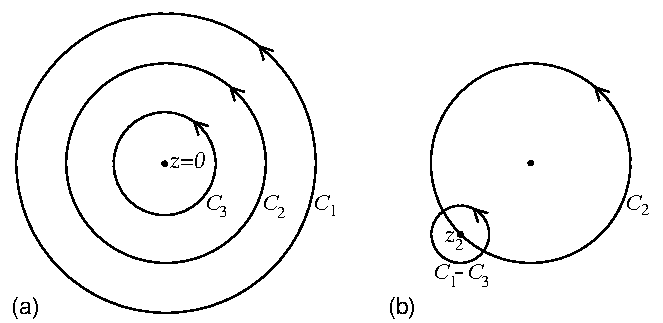
\includegraphics[width=0.8\linewidth]{figures/fig_2_4.pdf}
\caption{(a) $z=0$ を中心とする積分路。(b) 積分路 $C_2$ 上の $z_2$ を固定して、積分路 $C_1-C_3$ を縮める。}
\label{fig:2.4}
\end{figure}

この積分路の議論によって、OPE と交換関係を相互に行き来できる。強調しておくと、保存カレントについて OPE の特異項を知ることは、対応する電荷の交換子代数を知ることと等価である。図\ref{fig:2.4}の計算は、保存電荷 $Q_2\{C_2\}$ を任意の演算子で置き換えた場合にも成り立つ：
\begin{equation}
[Q,\mathcal A(z_2,\bar z_2)]
=\operatorname*{Res}_{z_1\to z_2}j(z_1)\mathcal A(z_2,\bar z_2)
=\frac1{i\epsilon}\delta\mathcal A(z_2,\bar z_2).
\tag{2.6.15}\label{eq:2.6.15}
\end{equation}
これは、電荷 $Q$ が対応する変換 $\delta$ を生成するという、よく知られた主張にほかならない。同様に、反正則カレントの周回積分
\begin{equation}
\widetilde Q\{C\}=-\oint_C\frac{d\bar z}{2\pi i}\,\widetilde j
\tag{2.6.16}\label{eq:2.6.16}
\end{equation}
については、Ward 恒等式と積分路の議論から
\begin{equation}
[\widetilde Q,\mathcal A(z_2,\bar z_2)]
=\operatorname*{Res}_{\bar z_1\to\bar z_2}
\widetilde j(\bar z_1)\mathcal A(z_2,\bar z_2)
=\frac1{i\epsilon}\delta\mathcal A(z_2,\bar z_2)
\tag{2.6.17}\label{eq:2.6.17}
\end{equation}
が従う。

これを Virasoro 生成子 \hyperref[eq:2.6.6]{(2.6.6)} に適用する。この場合、$j_m(z)=z^{m+1}T(z)$ である：
\begin{equation}
\begin{aligned}
&\operatorname*{Res}_{z_1\to z_2}
z_1^{m+1}T(z_1)\,z_2^{n+1}T(z_2)\\
&=\operatorname*{Res}_{z_1\to z_2}z_1^{m+1}z_2^{n+1}
\left(\frac{c}{2z_{12}^4}+\frac2{z_{12}^2}T(z_2)
+\frac1{z_{12}}\partial T(z_2)\right)\\
&=\frac c{12}(\partial^3z_2^{m+1})z_2^{n+1}
+2(\partial z_2^{m+1})z_2^{n+1}T(z_2)
+z_2^{m+n+2}\partial T(z_2)\\
&=\frac c{12}(m^3-m)z_2^{m+n-1}
+(m-n)z_2^{m+n+1}T(z_2)+\text{全微分}.
\end{aligned}
\tag{2.6.18}\label{eq:2.6.18}
\end{equation}
右辺を $z_2$ について周回積分すると、Virasoro 代数
\begin{equation}
[L_m,L_n]=(m-n)L_{m+n}
+\frac c{12}(m^3-m)\delta_{m,-n}
\tag{2.6.19}\label{eq:2.6.19}
\end{equation}
が得られる。$\widetilde L_m$ は中心電荷 $\widetilde c$ を持つ同じ代数を満たす。

したがって、どの CFT にも無限個の保存電荷である Virasoro 生成子が存在し、これらは Hilbert 空間に作用して代数 \hyperref[eq:2.6.19]{(2.6.19)} を満たす。ここではまず、いくつかの簡単な性質に注意しておこう。通常は $L_0$ と $\widetilde L_0$ の固有状態を用いる。生成子 $L_0$ は
\begin{equation}
[L_0,L_n]=-nL_n
\tag{2.6.20}\label{eq:2.6.20}
\end{equation}
を満たす。$\lvert\psi\rangle$ が固有値 $h$ の $L_0$ 固有状態ならば、
\begin{equation}
L_0L_n\lvert\psi\rangle
=L_n(L_0-n)\lvert\psi\rangle
=(h-n)L_n\lvert\psi\rangle,
\tag{2.6.21}\label{eq:2.6.21}
\end{equation}
なので、$L_n\lvert\psi\rangle$ は固有値 $h-n$ の固有状態である。$n<0$ の生成子は $L_0$ 固有値を上げ、$n>0$ の生成子は下げる。

三つの生成子 $L_0$ と $L_{\pm1}$ は、中心電荷を持たない閉じた代数をなす：
\begin{equation}
[L_0,L_1]=-L_1,\qquad
[L_0,L_{-1}]=L_{-1},\qquad
[L_1,L_{-1}]=2L_0.
\tag{2.6.22}\label{eq:2.6.22}
\end{equation}
これは $SL(2,\mathbb R)$ の代数であり、$SU(2)$ とは符号が異なる。ウェイト $(h,0)$ の正則テンソル場 $\mathcal O$ の Laurent 係数、
\begin{equation}
\mathcal O(z)=\sum_{m=-\infty}^{\infty}\frac{\mathcal O_m}{z^{m+h}},
\tag{2.6.23}\label{eq:2.6.23}
\end{equation}
については、OPE \hyperref[eq:2.4.16]{(2.4.16)} から交換関係
\begin{equation}
[L_m,\mathcal O_n]=[(h-1)m-n]\mathcal O_{m+n}
\tag{2.6.24}\label{eq:2.6.24}
\end{equation}
が得られる。ここでも $n>0$ のモードは $L_0$ を下げ、$n<0$ のモードは上げる。

開弦では、
\begin{equation}
0\leq\operatorname{Re}w\leq\pi
\quad\Longleftrightarrow\quad \operatorname{Im}z\geq0
\tag{2.6.25}\label{eq:2.6.25}
\end{equation}
とする。ただし $z=-\exp(-iw)$ である。これらの座標領域を図\ref{fig:2.5}に示す。境界では、エネルギー運動量テンソルは
\begin{equation}
T_{ab}n^at^b=0
\tag{2.6.26}\label{eq:2.6.26}
\end{equation}
を満たす。ここでも $n^a$ と $t^b$ は、それぞれ法線ベクトルと接線ベクトルである。これを見るには、境界が直線になる座標系を考える。境界の存在は法線方向の並進不変性を破るが、接線方向の並進不変性は破らないので、カレント $T_{ab}t^b$ はなお保存される。このとき境界条件 \hyperref[eq:2.6.26]{(2.6.26)} は、このカレントが境界の外へ流れ出す量がゼロであることを述べているにすぎない。今の場合、これは
\begin{equation}
\begin{gathered}
T_{ww}=T_{\bar w\bar w},\quad \operatorname{Re}w=0,\pi
\quad\Longleftrightarrow\quad
T_{zz}=T_{\bar z\bar z},\quad\operatorname{Im}z=0
\end{gathered}
\tag{2.6.27}\label{eq:2.6.27}
\end{equation}
となる。

\begin{figure}[htbp]
\centering
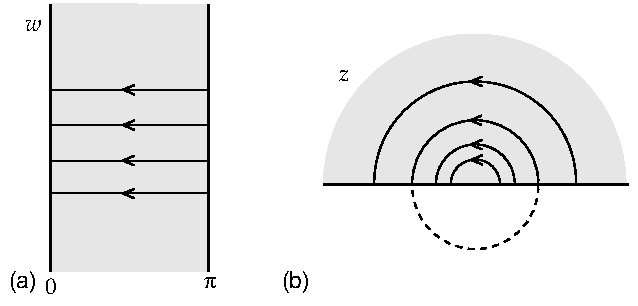
\includegraphics[width=0.8\linewidth]{figures/fig_2_5.pdf}
\caption{開弦の座標。(a) $w$ 平面の等時刻積分路。(b) $z$ 平面での同じ積分路。破線は、二重化の手法で用いる一つの積分路の延長を示す。}
\label{fig:2.5}
\end{figure}

二重化の手法を使うと便利である。$z$ 下半平面での $T_{zz}$ を、$z$ 上半平面にあるその鏡像点 $z'=\bar z$ での $T_{\bar z\bar z}$ の値によって定義する：
\begin{equation}
T_{zz}(z)\equiv T_{\bar z\bar z}(\bar z'),\qquad
\operatorname{Im}z<0.
\tag{2.6.28}\label{eq:2.6.28}
\end{equation}
すると運動方程式と境界条件は、$T_{zz}$ が複素平面全体で正則である、という主張にまとめられる。境界条件が $T$ と $\widetilde T$ を結びつけるので、Virasoro 生成子は一組しかない：
\begin{equation}
\begin{aligned}
L_m&=\frac1{2\pi i}\int_C
\left(dz\,z^{m+1}T_{zz}
-d\bar z\,\bar z^{m+1}T_{\bar z\bar z}\right)\\
&=\frac1{2\pi i}\oint dz\,z^{m+1}T_{zz}(z).
\end{aligned}
\tag{2.6.29}\label{eq:2.6.29}
\end{equation}
第1行の積分路 $C$ は原点を中心とする半円である。第2行では二重化の手法を使い、$L_m$ を閉じた積分路で表した。これらも Virasoro 代数
\begin{equation}
[L_m,L_n]=(m-n)L_{m+n}
+\frac c{12}(m^3-m)\delta_{m,-n}
\tag{2.6.30}\label{eq:2.6.30}
\end{equation}
を満たす。

\subsectionlink{モード展開}
\label{sec:2.7}
\subsubsectionlink*{自由スカラー}

自由場の理論では、場は調和振動子へと分解され、スペクトルとエネルギー運動量テンソルをモードによって表せる。まず閉弦から始める。$X^\mu$ 理論では、$\partial X$ と $\bar\partial X$ はそれぞれ正則および反正則であり、$T$ と同様の Laurent 展開を持つ：
\begin{equation}
\partial X^\mu(z)=-i\left(\frac{\alpha'}2\right)^{1/2}
\sum_{m=-\infty}^{\infty}\frac{\alpha_m^\mu}{z^{m+1}},
\qquad
\bar\partial X^\mu(\bar z)=-i\left(\frac{\alpha'}2\right)^{1/2}
\sum_{m=-\infty}^{\infty}\frac{\widetilde\alpha_m^\mu}{\bar z^{m+1}}.
\tag{2.7.1}\label{eq:2.7.1}
\end{equation}
同値な式として、
\begin{align}
\alpha_m^\mu&=\left(\frac2{\alpha'}\right)^{1/2}
\oint\frac{dz}{2\pi}\,z^m\partial X^\mu(z),
\tag{2.7.2a}\label{eq:2.7.2a}\\
\widetilde\alpha_m^\mu&=-\left(\frac2{\alpha'}\right)^{1/2}
\oint\frac{d\bar z}{2\pi}\,\bar z^m\bar\partial X^\mu(\bar z).
\tag{2.7.2b}\label{eq:2.7.2b}
\end{align}
$X^\mu$ の一価性から $\alpha_0^\mu=\widetilde\alpha_0^\mu$ が従う。さらに、時空並進の Noether カレントは $i\partial_aX^\mu/\alpha'$ なので、時空運動量は
\begin{equation}
p^\mu=\frac1{2\pi i}\oint_C
(dz\,j^\mu-d\bar z\,\widetilde j^\mu)
=\left(\frac2{\alpha'}\right)^{1/2}\alpha_0^\mu
=\left(\frac2{\alpha'}\right)^{1/2}\widetilde\alpha_0^\mu.
\tag{2.7.3}\label{eq:2.7.3}
\end{equation}
展開 \hyperref[eq:2.7.1]{(2.7.1)} を積分すると、
\begin{equation}
X^\mu(z,\bar z)=x^\mu-i\frac{\alpha'}2p^\mu\ln|z|^2
+i\left(\frac{\alpha'}2\right)^{1/2}
\sum_{\substack{m=-\infty\\m\ne0}}^\infty
\frac1m\left(\frac{\alpha_m^\mu}{z^m}
+\frac{\widetilde\alpha_m^\mu}{\bar z^m}\right).
\tag{2.7.4}\label{eq:2.7.4}
\end{equation}

通常の正準交換関係からでも、積分路の議論と $XX$ の OPE からでも、
\begin{align}
[\alpha_m^\mu,\alpha_n^\nu]
&=[\widetilde\alpha_m^\mu,\widetilde\alpha_n^\nu]
=m\delta_{m,-n}\eta^{\mu\nu},
\tag{2.7.5a}\label{eq:2.7.5a}\\
[x^\mu,p^\nu]&=i\eta^{\mu\nu}
\tag{2.7.5b}\label{eq:2.7.5b}
\end{align}
が導かれ、ほかの交換子はゼロとなる。スペクトルは、運動量 $k^\mu$ を持ち、すべての下降モード、すなわち $n>0$ の $\alpha_n^\mu$ によって消滅する状態 $\lvert0;k\rangle$ から始め、上昇モード（$n<0$）を可能なあらゆる仕方で作用させることで与えられる。

次に Virasoro 生成子をモード演算子によって展開したい。$X^\mu$ の Laurent 展開をエネルギー運動量テンソル \hyperref[eq:2.4.4]{(2.4.4)} に代入し、$z$ の同じべきの項を集めると、
\begin{equation}
L_m\sim\frac12\sum_{n=-\infty}^{\infty}
\alpha_{m-n}^\mu\alpha_{\mu n}.
\tag{2.7.6}\label{eq:2.7.6}
\end{equation}
$\sim$ は、演算子の順序を無視したことを示す。$m\ne0$ の場合、展開 \hyperref[eq:2.7.6]{(2.7.6)} はそのままで明確に定義され、正しい。各項のモード演算子同士は交換するので、順序は問題にならない。$m=0$ では、下降演算子を右に置き、正規順序定数を導入する：
\begin{equation}
L_0=\frac{\alpha'p^2}{4}
+\sum_{n=1}^\infty(\alpha_{-n}^\mu\alpha_{\mu n})+a^X.
\tag{2.7.7}\label{eq:2.7.7}
\end{equation}
第1.3節でも同じ問題に出会い、そのときは発見的な方法で扱った。今は、左辺には $:\ :$ 順序にしたエネルギー運動量テンソルの Laurent 係数という有限で曖昧さのない定義があるので、正規順序定数も有限で計算可能である。決め方はいくつかある。最も簡単なのは Virasoro 代数を用いるもので、
\begin{equation}
2L_0\lvert0;0\rangle
=(L_1L_{-1}-L_{-1}L_1)\lvert0;0\rangle=0,
\tag{2.7.8}\label{eq:2.7.8}
\end{equation}
したがって
\begin{equation}
a^X=0.
\tag{2.7.9}\label{eq:2.7.9}
\end{equation}
ここでは、既知の $L_1$ と $L_{-1}$ の形を用いた。それぞれの各項は、下降演算子か $p^\mu$ のどちらかを含むので、$\lvert0;0\rangle$ を消滅させる。

Virasoro 代数の中心電荷は OPE から決めた。モード演算子で表した Virasoro 生成子の式から直接決めることもできるが、少し注意が必要である。これは演習2.11とする。

新しい記法を導入しよう。記号 $\canorm{\phantom X}$ は生成・消滅演算子の正規順序を表し、すべての下降演算子をすべての上昇演算子の右に置き、反交換する演算子を入れ替えるたびに負号を付ける。この定義では、$p^\mu$ は下降演算子に、$x^\mu$ は上昇演算子に含める。この記法なら、$a^X=0$ なので
\begin{equation}
L_m=\frac12\sum_{n=-\infty}^{\infty}
\canorm{\alpha_{m-n}^\mu\alpha_{\mu n}}
\tag{2.7.10}\label{eq:2.7.10}
\end{equation}
と書ける。

これで二種類の正規順序を導入した。共形正規順序 $:\ :$（単に「正規順序」と呼ぶときはこれを意味する）と、生成・消滅演算子の正規順序 $\canorm{\phantom X}$ である。前者は、OPE と共形変換性が簡単な演算子を与える点で便利である。読者にはおそらく後者の方がなじみ深いだろうが、こちらは演算子の行列要素を求めるのに便利である。この二つの関係を求めよう。まず時間順序積と生成・消滅演算子の正規順序積を比較する。$|z|>|z'|$ を満たす積 $X^\mu(z,\bar z)X^\nu(z',\bar z')$ にモード展開を代入し、$X^\mu(z,\bar z)$ に含まれる下降演算子を右へ動かす。交換子を追跡すると、
\begin{equation}
\begin{aligned}
X^\mu(z,\bar z)X^\nu(z',\bar z')
&=\canorm{X^\mu(z,\bar z)X^\nu(z',\bar z')}\\
&\quad+\frac{\alpha'}2\eta^{\mu\nu}
\left[-\ln|z|^2+\sum_{m=1}^{\infty}\frac1m
\left(\frac{z'^m}{z^m}+\frac{\bar z'^m}{\bar z^m}\right)\right]\\
&=\canorm{X^\mu(z,\bar z)X^\nu(z',\bar z')}
-\frac{\alpha'}2\eta^{\mu\nu}\ln|z-z'|^2.
\end{aligned}
\tag{2.7.11}\label{eq:2.7.11}
\end{equation}
$|z|>|z'|$ なので、ここで左辺は時間順序積であり、和は収束する。定義 \hyperref[eq:2.1.21a]{(2.1.21)} は、時間順序積と共形正規順序積の関係を与えていた（式 \hyperref[eq:2.1.21a]{(2.1.21)} は経路積分の言葉で書かれていたので、その右辺の積は演算子形式では時間順序積になる）。それは関係 \hyperref[eq:2.7.11]{(2.7.11)} と同じなので、
\begin{equation}
\canorm{X^\mu(z,\bar z)X^\nu(z',\bar z')}
=:X^\mu(z,\bar z)X^\nu(z',\bar z'):.
\tag{2.7.12}\label{eq:2.7.12}
\end{equation}
このような関係は一般の CFT では成立しない。実際、$p^\mu$ を下降演算子と一緒に分類した多少恣意的な選択は、この簡単な結果を得ることも目的の一つであった。また、たとえば $z$ ではなく $w$ について共形正規順序にした演算子でも、この関係は成立しない。式 \hyperref[eq:2.7.12]{(2.7.12)} からモード展開 \hyperref[eq:2.7.10]{(2.7.10)} を直ちに書け、$a^X=0$ の二つ目の導出が得られる。

三つ以上の $X^\mu$ の生成・消滅演算子の正規順序積は、$:\ :$ 順序と同じ組み合わせ論的性質を持つ。すなわち、すべての差し引きについて和を取ることで時間順序積から得られる。これは場の理論の Wick の定理である。また、ある正規順序で定義した演算子を別の正規順序へ変換するには、2点関数の差を用いてすべての差し引きについて和を取ればよい。すなわち、二種類の順序が
\begin{equation}
[X^\mu(z,\bar z)X^\nu(z',\bar z')]_1
=[X^\mu(z,\bar z)X^\nu(z',\bar z')]_2
+\eta^{\mu\nu}\Delta(z,\bar z,z',\bar z')
\tag{2.7.13}\label{eq:2.7.13}
\end{equation}
を満たすならば、一般の演算子 $\mathcal F$ について
\begin{equation}
[\mathcal F]_1=
\exp\left(\frac12\int d^2z\,d^2z'\,
\Delta(z,\bar z,z',\bar z')
\frac{\delta}{\delta X^\mu(z,\bar z)}
\frac{\delta}{\delta X_\mu(z',\bar z')}\right)[\mathcal F]_2.
\tag{2.7.14}\label{eq:2.7.14}
\end{equation}

線形ディラトン CFT では、Laurent 展開と交換関係は変わらないが、Virasoro 生成子に追加項が含まれる：
\begin{equation}
L_m=\frac12\sum_{n=-\infty}^\infty
\canorm{\alpha_{m-n}^\mu\alpha_{\mu n}}
+i\left(\frac{\alpha'}2\right)^{1/2}(m+1)V^\mu\alpha_{\mu m}.
\tag{2.7.15}\label{eq:2.7.15}
\end{equation}

\subsubsectionlink*{\texorpdfstring{$bc$}{bc} CFT}

場 $b$ と $c$ は Laurent 展開
\begin{equation}
b(z)=\sum_{m=-\infty}^\infty\frac{b_m}{z^{m+\lambda}},
\qquad
c(z)=\sum_{m=-\infty}^\infty\frac{c_m}{z^{m+1-\lambda}}
\tag{2.7.16}\label{eq:2.7.16}
\end{equation}
を持つ。厳密には、これらが Laurent 展開となるのは $\lambda$ が整数の場合だけであり、ここではそう仮定する。半整数の場合も興味深いが、第10章で詳しく扱う。OPE から反交換関係
\begin{equation}
\{b_m,c_n\}=\delta_{m,-n}
\tag{2.7.17}\label{eq:2.7.17}
\end{equation}
が得られる。まず、すべての $n>0$ の演算子によって消滅する状態を考える。$b_0,c_0$ の振動子代数は、そのような基底状態を二つ、$\lvert\downarrow\rangle$ と $\lvert\uparrow\rangle$、生成する。これらの性質は
\begin{align}
b_0\lvert\downarrow\rangle&=0,\qquad
b_0\lvert\uparrow\rangle=\lvert\downarrow\rangle,
\tag{2.7.18a}\label{eq:2.7.18a}\\
c_0\lvert\downarrow\rangle&=\lvert\uparrow\rangle,\qquad
c_0\lvert\uparrow\rangle=0,
\tag{2.7.18b}\label{eq:2.7.18b}\\
b_n\lvert\downarrow\rangle&=b_n\lvert\uparrow\rangle
=c_n\lvert\downarrow\rangle=c_n\lvert\uparrow\rangle=0,\qquad n>0.
\tag{2.7.18c}\label{eq:2.7.18c}
\end{align}
一般の状態は、これらの状態に $n<0$ のモードを各々高々一度ずつ作用させて得られる（これらは反交換するためである）。後に明らかになる理由により、$b_0$ を下降演算子に、$c_0$ を上昇演算子に分類するのが慣例なので、$\lvert\downarrow\rangle$ をゴースト真空 $\lvert0\rangle$ として特別に選ぶ。弦理論では、どちらも $\lambda=2$ の正則な $bc$ 理論と反正則な $\widetilde b\widetilde c$ 理論を持つ。したがって閉弦のスペクトルには、上の系を二つ複製したものの積が含まれる。

Virasoro 生成子は
\begin{equation}
L_m=\sum_{n=-\infty}^\infty(m\lambda-n)
\canorm{b_nc_{m-n}}+\delta_{m,0}a^{\mathrm g}.
\tag{2.7.19}\label{eq:2.7.19}
\end{equation}
順序定数は式 \hyperref[eq:2.7.8]{(2.7.8)} と同じように決められ、
\begin{equation}
\begin{aligned}
2L_0\lvert\downarrow\rangle
&=(L_1L_{-1}-L_{-1}L_1)\lvert\downarrow\rangle\\
&=(\lambda b_0c_1)[(1-\lambda)b_{-1}c_0]\lvert\downarrow\rangle
=\lambda(1-\lambda)\lvert\downarrow\rangle.
\end{aligned}
\tag{2.7.20}\label{eq:2.7.20}
\end{equation}
したがって $a^{\mathrm g}=\frac12\lambda(1-\lambda)$ であり、
\begin{equation}
L_m=\sum_{n=-\infty}^\infty(m\lambda-n)
\canorm{b_nc_{m-n}}+\frac{\lambda(1-\lambda)}2\delta_{m,0}.
\tag{2.7.21}\label{eq:2.7.21}
\end{equation}
この定数は、この CFT における $:\ :$ と $\canorm{\phantom X}$ の関係を求めることでも得られる（演習2.13、2.14）。

ゴースト数カレント \hyperref[eq:2.5.14]{(2.5.14)}、$j=-:bc:$ の電荷は
\begin{equation}
\begin{aligned}
N^{\mathrm g}&=-\frac1{2\pi i}\int_0^{2\pi}dw\,j_w\\
&=\sum_{n=1}^\infty(c_{-n}b_n-b_{-n}c_n)+c_0b_0-\frac12.
\end{aligned}
\tag{2.7.22}\label{eq:2.7.22}
\end{equation}
これは
\begin{equation}
[N^{\mathrm g},b_m]=-b_m,\qquad
[N^{\mathrm g},c_m]=c_m
\tag{2.7.23}\label{eq:2.7.23}
\end{equation}
を満たすので、$c$ の励起数から $b$ の励起数を引いたものを数える。基底状態のゴースト数は $\pm\frac12$ である：
\begin{equation}
N^{\mathrm g}\lvert\downarrow\rangle=-\frac12\lvert\downarrow\rangle,
\qquad
N^{\mathrm g}\lvert\uparrow\rangle=\frac12\lvert\uparrow\rangle.
\tag{2.7.24}\label{eq:2.7.24}
\end{equation}
これは演習2.13で求める順序定数の値に依存するが、基底状態の平均ゴースト数はゼロになるべきだという理由から推測することもできる。ゴースト数は $b\leftrightarrow c$ の下で符号を変えるからである。

$\beta\gamma$ 理論も同様である。詳細は、それが必要になる第10章まで先送りする。

\subsubsectionlink*{開弦}

開弦では、Neumann 境界条件は実軸上で $\partial_zX^\mu=\partial_{\bar z}X^\mu$ となる。境界条件は展開 \hyperref[eq:2.7.1]{(2.7.1)} で $\alpha_m^\mu=\widetilde\alpha_m^\mu$ を要求するので、モードは一組しかない。時空運動量の積分 \hyperref[eq:2.7.3]{(2.7.3)} は半円上だけを走るため、規格化は今度は
\begin{equation}
\alpha_0^\mu=(2\alpha')^{1/2}p^\mu.
\tag{2.7.25}\label{eq:2.7.25}
\end{equation}
したがって $X^\mu$ の展開は
\begin{equation}
X^\mu(z,\bar z)=x^\mu-i\alpha'p^\mu\ln|z|^2
+i\left(\frac{\alpha'}2\right)^{1/2}
\sum_{\substack{m=-\infty\\m\ne0}}^\infty
\frac{\alpha_m^\mu}{m}(z^{-m}+\bar z^{-m}).
\tag{2.7.26}\label{eq:2.7.26}
\end{equation}
また、
\begin{equation}
L_0=\alpha'p^2+\sum_{n=1}^\infty\alpha_{-n}^\mu\alpha_{\mu n}.
\tag{2.7.27}\label{eq:2.7.27}
\end{equation}
交換関係は以前と同じである：
\begin{equation}
[\alpha_m^\mu,\alpha_n^\nu]=m\delta_{m,-n}\eta^{\mu\nu},
\qquad [x^\mu,p^\nu]=i\eta^{\mu\nu}.
\tag{2.7.28}\label{eq:2.7.28}
\end{equation}

$bc$ 理論では、弦に関係する境界条件は、境界が実軸となる $z$ 座標を用いて
\begin{equation}
c(z)=\widetilde c(\bar z),\qquad
b(z)=\widetilde b(\bar z),\qquad\operatorname{Im}z=0
\tag{2.7.29}\label{eq:2.7.29}
\end{equation}
と書かれる。すると二重化の手法によって、上半平面の正則場と反正則場を、全平面の正則場として表せる：
\begin{equation}
c(z)\equiv\widetilde c(\bar z'),\qquad
b(z)\equiv\widetilde b(\bar z'),\qquad
\operatorname{Im}z\leq0,\quad z'=\bar z.
\tag{2.7.30}\label{eq:2.7.30}
\end{equation}
したがって開弦は、$b$ と $c$ について、それぞれ一組の Laurent モードを持つ。

\subsectionlink{頂点演算子}
\label{sec:2.8}

場の量子論には、一方で理論の状態空間があり、他方で局所演算子の集合がある。共形場理論では、CFT を円上で量子化すると、これらの間に簡単で有用な同型対応がある。$w$ 座標で半無限円筒
\begin{equation}
0\leq\operatorname{Re}w\leq2\pi,\qquad
w\sim w+2\pi,\qquad \operatorname{Im}w\leq0
\tag{2.8.1}\label{eq:2.8.1}
\end{equation}
を考える。これは座標 $z=\exp(-iw)$ では単位円板に写る。その様子を図\ref{fig:2.6}に示す。$w$ 座標で経路積分を定義するには、とくに $\operatorname{Im}w\to-\infty$ での境界条件を指定しなければならない。すなわち、初期状態を指定する必要がある。$z$ 座標では $\operatorname{Im}w=-\infty$ は原点に写るので、これはその点での場の振る舞いを指定することと同じである。実質的には、これにより原点に局所演算子を定義しており、その状態に対応する頂点演算子と呼ばれる。逆向きに進むと、原点に演算子 $\mathcal A$ を置いた円板上の経路積分は、初期状態 $\lvert\mathcal A\rangle$ を指定した円筒上の経路積分に写る。

自由場の理論では、この同型対応の具体的な形を容易に求められる。図\ref{fig:2.6}(a) のように、保存電荷 $Q$ が状態 $\lvert\mathcal A\rangle$ に作用しているとする。図\ref{fig:2.6}(b) の周回積分を OPE で評価すれば、対応する局所演算子を求められる。これを使い、単位演算子に対応する状態 $\lvert1\rangle$ を同定しよう。原点に演算子がなければ、$\partial X^\mu$ と $\bar\partial X^\mu$ は図\ref{fig:2.6}(b) の $Q$ の積分路の内部で、それぞれ正則および反正則である。したがって、$m\geq0$ の $\alpha_m^\mu$ と $\widetilde\alpha_m^\mu$ を定義する周回積分 \hyperref[eq:2.7.2a]{(2.7.2)} には極がなく、ゼロになる。つまり、$\lvert1\rangle$ はこれらのモードによって消滅する。これにより、この状態が基底状態であると分かる：
\begin{equation}
\lvert1\rangle=\lvert0;0\rangle.
\tag{2.8.2}\label{eq:2.8.2}
\end{equation}
規格化は便宜上このように選んだ。

\begin{figure}[htbp]
\centering
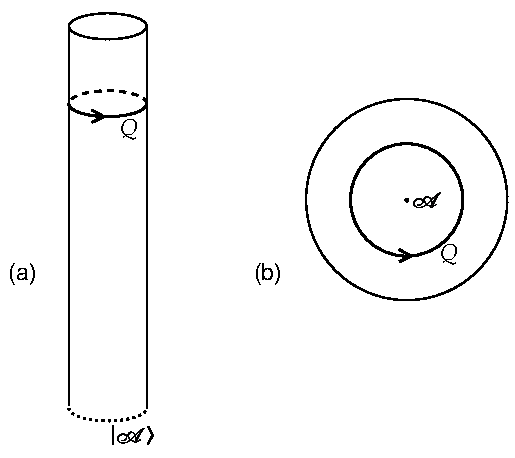
\includegraphics[width=0.8\linewidth]{figures/fig_2_6.pdf}
\caption{(a) 初期状態 $\lvert\mathcal A\rangle$ と電荷 $Q$ を持つ、$w$ での半無限円筒。(b) それと共形的に等価な単位円板。局所演算子 $\mathcal A$ と、$Q$ の周回積分を示す。}
\label{fig:2.6}
\end{figure}

次に、たとえば $m$ が正の状態 $\alpha_{-m}^\mu\lvert1\rangle$ を考える。図\ref{fig:2.6}(b) に移り、$Q=\alpha_{-m}^\mu$ が単位演算子を囲むようにすると、場は積分路の内部で正則なので、$m\geq1$ について
\begin{equation}
\alpha_{-m}^\mu=
\left(\frac2{\alpha'}\right)^{1/2}
\oint\frac{dz}{2\pi}\,z^{-m}\partial X^\mu(z)
\ \longrightarrow\
\left(\frac2{\alpha'}\right)^{1/2}
\frac{i}{(m-1)!}\partial^m X^\mu(0)
\tag{2.8.3}\label{eq:2.8.3}
\end{equation}
と評価できる。したがって、
\begin{equation}
\alpha_{-m}^\mu\lvert1\rangle\cong
\left(\frac2{\alpha'}\right)^{1/2}
\frac{i}{(m-1)!}\partial^m X^\mu(0),\qquad m\geq1.
\tag{2.8.4}\label{eq:2.8.4}
\end{equation}
同様に、
\begin{equation}
\widetilde\alpha_{-m}^\mu\lvert1\rangle\cong
\left(\frac2{\alpha'}\right)^{1/2}
\frac{i}{(m-1)!}\bar\partial^m X^\mu(0),\qquad m\geq1.
\tag{2.8.5}\label{eq:2.8.5}
\end{equation}

この対応は、$\alpha_{-m}^\mu$ または $\widetilde\alpha_{-m}^\mu$ が一般の状態 $\lvert\mathcal A\rangle$ に作用する場合にも成立する。$: \mathcal A(0,0):$ を任意の正規順序演算子とすると、$\partial X^\mu(z)$ と $:\mathcal A(0,0):$ の演算子積には特異性があり得るが、$m>0$ について
\begin{equation}
\alpha_{-m}^\mu:\mathcal A(0,0):
=:\alpha_{-m}^\mu\mathcal A(0,0):
\tag{2.8.6}\label{eq:2.8.6}
\end{equation}
を確かめるのは難しくない。縮約の周回積分には決して1位の極が現れないからである。したがって、同じ操作 \hyperref[eq:2.8.3]{(2.8.3)} を正規順序の内部で行え、複数の $\alpha$ 振動子を励起した状態は、対応する演算子の $:\ :$ 正規順序積となる：
\begin{align}
\alpha_{-m}^\mu&\longrightarrow
i\left(\frac2{\alpha'}\right)^{1/2}
\frac1{(m-1)!}\partial^mX^\mu(0),\qquad m\geq1,
\tag{2.8.7a}\label{eq:2.8.7a}\\
\widetilde\alpha_{-m}^\mu&\longrightarrow
i\left(\frac2{\alpha'}\right)^{1/2}
\frac1{(m-1)!}\bar\partial^mX^\mu(0),\qquad m\geq1.
\tag{2.8.7b}\label{eq:2.8.7b}
\end{align}
同様に、
\begin{equation}
x_0^\mu\longrightarrow X^\mu(0,0).
\tag{2.8.8}\label{eq:2.8.8}
\end{equation}
どの状態も、式 \hyperref[eq:2.8.7a]{(2.8.7)} と \hyperref[eq:2.8.8]{(2.8.8)} の左辺の演算子を $\lvert1\rangle$ に作用させて得られる。すると、この状態に対応する演算子は、右辺の対応する局所演算子の $:\ :$ 正規順序積で与えられる。たとえば、
\begin{equation}
\lvert0;k\rangle\cong:e^{ik\cdot X(0,0)}:.
\tag{2.8.9}\label{eq:2.8.9}
\end{equation}
これは容易に理解できる。並進 $X^\mu\to X^\mu+a^\mu$ の下で、状態と対応する演算子はどちらも $\exp(ik\cdot a)$ を掛けるという同じ変換を受けるからである。

同じ方法は $bc$ 理論にも適用できる。明確さのため、ボース弦理論で関心のある $\lambda=2$ の場合に限定し、一般化は読者に任せる。Laurent 展開 \hyperref[eq:2.7.16]{(2.7.16)} と積分路の議論から、
\begin{equation}
b_m\lvert1\rangle=0,\quad m\geq-1,\qquad
c_m\lvert1\rangle=0,\quad m\geq2
\tag{2.8.10}\label{eq:2.8.10}
\end{equation}
が従う。$b$ と $c$ の共形ウェイトにより Laurent 展開の指数がずれるため、単位演算子はもはや基底状態へは写らないことに注意しよう。代わりに、関係 \hyperref[eq:2.8.10]{(2.8.10)} から
\begin{equation}
\lvert1\rangle=b_{-1}\lvert\downarrow\rangle
\tag{2.8.11}\label{eq:2.8.11}
\end{equation}
と決まる。上昇演算子の対応を求めるのは容易で、
\begin{align}
b_{-m}&\longrightarrow\frac1{(m-2)!}\partial^{m-2}b(0),
\qquad m\geq2,
\tag{2.8.12a}\label{eq:2.8.12a}\\
c_{-m}&\longrightarrow\frac1{(m+1)!}\partial^{m+1}c(0),
\qquad m\geq-1.
\tag{2.8.12b}\label{eq:2.8.12b}
\end{align}

ゴースト数 $-\frac32$ の状態 $b_{-1}\lvert\downarrow\rangle$ がゴースト数0の単位演算子に写り、ゴースト数 $-\frac12$ の状態 $\lvert\downarrow\rangle$ がゴースト数1の演算子 $c$ に写ることに注意しよう。この差は、ゴースト数カレントのテンソル的でない性質 \hyperref[eq:2.5.17]{(2.5.17)}、
\begin{equation}
(\partial_z w)j_w(w)=j_z(z)
+q_0\frac{\partial_z^2w}{\partial_z w}
=j_z(z)-\frac{q_0}{z}
\tag{2.8.13}\label{eq:2.8.13}
\end{equation}
から生じる。ここで $q_0=\lambda-\frac12=\frac32$ である。状態のゴースト数は慣例として円筒座標系の式 $N^{\mathrm g}$、式 \hyperref[eq:2.7.22]{(2.7.22)}、で定義する。一方、図\ref{fig:2.6}の積分路の議論が頂点演算子のゴースト数に結びつけるのは、動径座標系の電荷
\begin{equation}
Q^{\mathrm g}\equiv\frac1{2\pi i}\oint dz\,j_z
=N^{\mathrm g}+q_0
\tag{2.8.14}\label{eq:2.8.14}
\end{equation}
である。これはほかの電荷にも当てはまる。テンソルカレントなら、状態と対応する演算子の電荷は等しい。

以上の大部分は $\beta\gamma$ 理論にも拡張できるが、超弦にはいくつかの複雑な点があるので、第10章まで先送りする。

この節の考え方はすべて開弦にも拡張できる。半無限帯
\begin{equation}
0\leq\operatorname{Re}w\leq\pi,\qquad \operatorname{Im}w\leq0
\tag{2.8.15}\label{eq:2.8.15}
\end{equation}
は $z=-\exp(-iw)$ によって、上半平面と単位円の内部の共通部分である半円板に写る。初期状態はここでも原点に写るが、原点は境界上にあるため、同型対応
\begin{equation}
\text{境界上の局所演算子}
\quad\longleftrightarrow\quad
\text{区間上の状態}
\tag{2.8.16}\label{eq:2.8.16}
\end{equation}
がある。上の議論と並行する詳細は読者に任せる。ここでも、場を正則性によって下半平面へ拡張する二重化の手法が、積分路の議論を行うのに便利である。

\subsubsectionlink*{経路積分による導出}

状態と演算子の同型対応は重要だがなじみの薄い考え方なので、より明示的な経路積分による導出も与えておくと有用である。$z$ 平面の単位円板を考え、原点に局所演算子 $\mathcal A$ を置き、経路積分の場 $\phi$ を単位円上である特定の境界値 $\phi_{\mathrm b}$ に固定する。$\phi_{\mathrm b}$ を固定したまま、円板の内部の場 $\phi_{\mathrm i}$ について経路積分すると、ある汎関数 $\Psi_{\mathcal A}[\phi_{\mathrm b}]$ が得られる：
\begin{equation}
\Psi_{\mathcal A}[\phi_{\mathrm b}]
=\int[d\phi_{\mathrm i}]_{\phi_{\mathrm b}}\,
\exp(-S[\phi_{\mathrm i}])\mathcal A(0).
\tag{2.8.17}\label{eq:2.8.17}
\end{equation}
場の汎関数は状態の Schrödinger 表現なので、これは演算子から状態への写像である。各場の配位に複素振幅を割り当てる Schrödinger 表現には、多くの用途がある。場の理論の教科書ではしばしば Fock 空間表示に重点が置かれ、Schrödinger 表現は省かれる。

逆向きに進むには、ある状態 $\Psi[\phi_{\mathrm b}]$ から始める。外側の円上の場 $\phi_{\mathrm b}$ を固定し、内側の円上の場 $\phi'_{\mathrm b}$ を次のように積分する、環状領域 $1\geq|z|\geq r$ 上の経路積分を考える：
\begin{equation}
\int[d\phi'_{\mathrm b}]
[d\phi_{\mathrm i}]_{\phi_{\mathrm b},\phi'_{\mathrm b}}
\exp(-S[\phi_{\mathrm i}])\,
r^{-L_0-\widetilde L_0}\Psi[\phi'_{\mathrm b}].
\tag{2.8.18}\label{eq:2.8.18}
\end{equation}
すなわち、積分は状態（汎関数）$r^{-L_0-\widetilde L_0}\Psi[\phi'_{\mathrm b}]$ によって重み付けされる。さて、環状領域上の経路積分は、$|z|=r$ から $|z|=1$ への伝播にほかならず、演算子 $r^{+L_0+\widetilde L_0}$ の作用と同じである。これが $\Psi$ に作用している演算子を打ち消すので、経路積分 \hyperref[eq:2.8.18]{(2.8.18)} は再び $\Psi[\phi_{\mathrm b}]$ となる。ここで $r\to0$ の極限を取る。環状領域は円板となり、内側の円上の経路積分の極限は、原点にある局所演算子を定義すると考えられる。構成の仕方から、この演算子を挿入した円板上の経路積分は、境界に $\Psi[\phi_{\mathrm b}]$ を再現する。

一つの自由スカラー場 $X$ について、これを具体的に計算しよう。単位円上で
\begin{equation}
X_{\mathrm b}(\theta)=\sum_{n=-\infty}^\infty X_ne^{in\theta},
\qquad X_n^*=X_{-n}
\tag{2.8.19}\label{eq:2.8.19}
\end{equation}
と展開する。したがって、境界状態 $\Psi[X_{\mathrm b}]$ は、すべての $X_n$ の関数とみなせる。まず、挿入のない経路積分
\begin{equation}
\Psi_1[X_{\mathrm b}]
=\int[dX_{\mathrm i}]_{X_{\mathrm b}}\,
\exp\left(-\frac1{2\pi\alpha'}
\int d^2z\,\partial X\bar\partial X\right)
\tag{2.8.20}\label{eq:2.8.20}
\end{equation}
によって与えられる、単位演算子に対応する状態を同定しよう。これを通常の Gauss 積分の方法で評価する。$X_{\mathrm i}$ を古典的な部分とゆらぎに分ける：
\begin{align}
X_{\mathrm i}&=X_{\mathrm{cl}}+X'_{\mathrm i},
\tag{2.8.21a}\label{eq:2.8.21a}\\
X_{\mathrm{cl}}(z,\bar z)
&=X_0+\sum_{n=1}^\infty(z^nX_n+\bar z^nX_{-n}).
\tag{2.8.21b}\label{eq:2.8.21b}
\end{align}
この定義によって、$X_{\mathrm{cl}}$ は運動方程式を満たし、$X'_{\mathrm i}$ は境界でゼロになる。すると経路積分は分離され、
\begin{equation}
\Psi_1[X_{\mathrm b}]=\exp(-S_{\mathrm{cl}})
\int[dX'_{\mathrm i}]_{X_{\mathrm b}=0}\,
\exp\left(-\frac1{2\pi\alpha'}
\int d^2z\,\partial X'\bar\partial X'\right),
\tag{2.8.22}\label{eq:2.8.22}
\end{equation}
ここで
\begin{equation}
\begin{aligned}
S_{\mathrm{cl}}&=\frac1{2\pi\alpha'}
\sum_{m,n=1}^\infty mnX_mX_{-n}
\int_{|z|<1}d^2z\,z^{m-1}\bar z^{n-1}\\
&=\frac1{\alpha'}\sum_{m=1}^\infty mX_mX_{-m}.
\end{aligned}
\tag{2.8.23}\label{eq:2.8.23}
\end{equation}
$X'_{\mathrm i}$ の積分は境界条件に依存しない定数なので、
\begin{equation}
\Psi_1[X_{\mathrm b}]\propto
\exp\left(-\frac1{\alpha'}\sum_{m=1}^\infty mX_mX_{-m}\right).
\tag{2.8.24}\label{eq:2.8.24}
\end{equation}
これは Gauss 関数であり、実際に基底状態である。このことを見るため、上昇演算子と下降演算子を Schrödinger 基底で書く：
\begin{align}
\alpha_n&=-\frac{in}{(2\alpha')^{1/2}}X_{-n}
-i\left(\frac{\alpha'}2\right)^{1/2}\frac{\partial}{\partial X_n},
\tag{2.8.25a}\label{eq:2.8.25a}\\
\widetilde\alpha_n&=-\frac{in}{(2\alpha')^{1/2}}X_n
-i\left(\frac{\alpha'}2\right)^{1/2}\frac{\partial}{\partial X_{-n}}.
\tag{2.8.25b}\label{eq:2.8.25b}
\end{align}
これは $|z|=1$ での Laurent 展開とモード代数から従う。\hyperref[eq:2.8.24]{(2.8.24)} に作用させると、
\begin{equation}
\alpha_n\Psi_1[X_{\mathrm b}]
=\widetilde\alpha_n\Psi_1[X_{\mathrm b}]=0,\qquad n\geq0
\tag{2.8.26}\label{eq:2.8.26}
\end{equation}
となるので、これは確かに基底状態である。したがって、
\begin{equation}
\lvert1\rangle\propto\lvert0;0\rangle.
\tag{2.8.27}\label{eq:2.8.27}
\end{equation}
ここで経路積分全体の規格化を追跡しようとする代わりに、$\lvert1\rangle=\lvert0;0\rangle$ と定義する。

もう一つ容易に計算できるのは、$\partial^kX$ に対応する状態である。これは結果に $\partial^kX_{\mathrm{cl}}(0)=k!X_k$ という因子を付け加えるだけなので、
\begin{equation}
\lvert\partial^kX\rangle=k!X_k\Psi_1
=-i\left(\frac{\alpha'}2\right)^{1/2}
(k-1)!\alpha_{-k}\lvert0;0\rangle,
\tag{2.8.28}\label{eq:2.8.28}
\end{equation}
となり、$\bar\partial^kX$ についても同様である。これは $X$ の指数関数と微分のあらゆる積へ拡張できる。共形正規順序は、ちょうど $X'_{\mathrm i}$ の経路積分の効果を打ち消す。

\subsectionlink{状態と演算子についてさらに}
\label{sec:2.9}
\subsubsectionlink*{OPE}

この節では、状態と演算子の対応をさらに応用する。最初は、図\ref{fig:2.7}に示す OPE の簡単で一般的な導出である。$|z|<1$ として、積
\begin{equation}
\mathcal A_i(z,\bar z)\mathcal A_j(0,0)
\tag{2.9.1}\label{eq:2.9.1}
\end{equation}
を考える。経路積分を、単位円板の内部の場 $\phi_{\mathrm i}$ の積分、単位円上の場 $\phi_{\mathrm b}$ の積分、および単位円板の外部の場 $\phi_{\mathrm e}$ の積分に分けられる。このように経路積分を切り開くことは付録で詳しく論じる。前節の最後の議論と同様に、$\phi_{\mathrm i}$ の積分の後には $\phi_{\mathrm b}$ のある汎関数が残る。それを $\Psi_{ij,z,\bar z}[\phi_{\mathrm b}]$ と呼ぼう。状態と演算子の対応によれば、これは適切な局所演算子 $\mathcal A_{ij,z,\bar z}(0,0)$ を入れた円板を貼り戻すことと等価であり、これで導出は終わりである。標準的な形にするため、$L_0,\widetilde L_0$ の固有状態の完全系で展開する：
\begin{equation}
\mathcal A_{ij,z,\bar z}
=\sum_k z^{h_k-h_i-h_j}
\bar z^{\widetilde h_k-\widetilde h_i-\widetilde h_j}
c^k_{ij}\mathcal A_k.
\tag{2.9.2}\label{eq:2.9.2}
\end{equation}
$z$ と $\bar z$ への依存性は、式 \hyperref[eq:2.4.20]{(2.4.20)} と同じく共形ウェイトによって決まる。OPE の収束は、量子力学における完全系の通常の収束にほかならない。この構成は、$|z'|\leq|z|$ を満たすほかの演算子が存在せず、半径 $|z|+\epsilon$ の円で切れる限り可能である。

\begin{figure}[htbp]
\centering
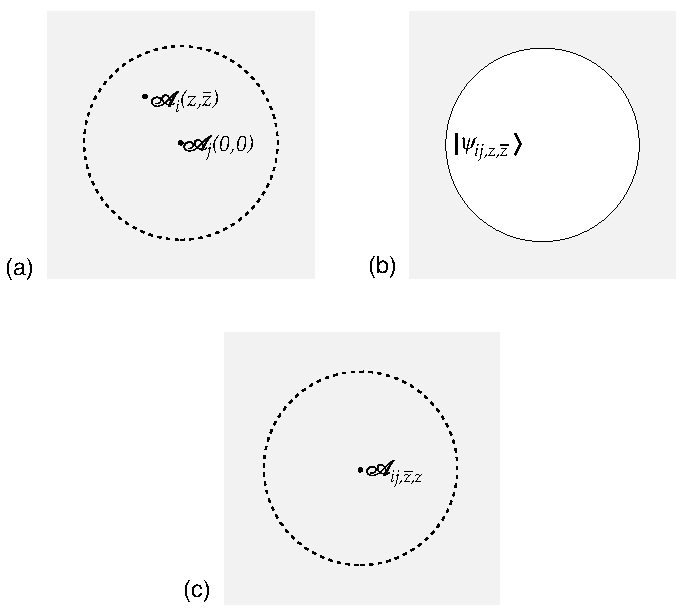
\includegraphics[width=0.8\linewidth]{figures/fig_2_7.pdf}
\caption{(a) 二つの局所演算子を持つ世界面。(b) 円板の内部の場を積分すると、境界状態 $\lvert\psi_{ij,z,\bar z}\rangle$ が得られる。(c) 対応する局所演算子を持つ円板を縫い合わせる。確定したウェイトを持つ演算子で展開すると OPE が得られる。}
\label{fig:2.7}
\end{figure}

三つの演算子
\begin{equation}
\mathcal A_i(0,0)\mathcal A_j(1,1)\mathcal A_k(z,\bar z)
\tag{2.9.3}\label{eq:2.9.3}
\end{equation}
について、$z\to0$ と $z\to1$ の OPE の収束領域 $|z|<1$ と $|1-z|<1$ は重なり合う。このとき三重積における $\mathcal A_m$ の係数は、$c^l_{ik}c^m_{lj}$ を含む和としても、$c^l_{jk}c^m_{li}$ を含む和としても書ける。結合則は、これらの和が等しいことを要求する。これを模式的に示したのが図\ref{fig:2.8}である。

\begin{figure}[htbp]
\centering
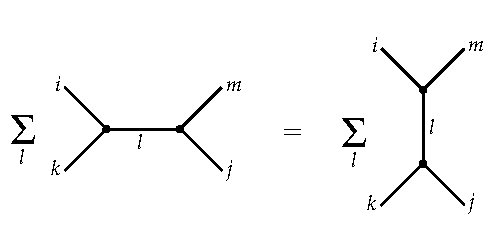
\includegraphics[width=0.8\linewidth]{figures/fig_2_8.pdf}
\caption{OPE の結合則の模式図。}
\label{fig:2.8}
\end{figure}

\subsubsectionlink*{Virasoro 代数と最高ウェイト状態}

今度は Virasoro 生成子について、図\ref{fig:2.6}の議論を考える：
\begin{equation}
\begin{aligned}
L_m\lvert\mathcal A\rangle
&\cong\oint\frac{dz}{2\pi i}\,
z^{m+1}T(z)\mathcal A(0,0)\\
&\cong L_m\cdot\mathcal A(0,0).
\end{aligned}
\tag{2.9.4}\label{eq:2.9.4}
\end{equation}
ここでは新しい考え方と記法を導入した。状態と演算子の同型対応により、Hilbert 空間に作用するすべての演算子には、局所演算子の空間に作用する像がある。言い換えれば、演算子を囲む対応する積分路を取り、その結果生じる局所演算子を OPE で評価するのである。状態を状態に写す $L_m$ に対応するのが、局所演算子を局所演算子に写す $L_m\cdot$ である。一般にはさまざまな位置 $z_i$ に局所演算子があり、各演算子の位置を中心に Laurent 展開して得られる、それぞれ別の Virasoro 代数の複製が存在する。幾何形状によっては、円筒における $z=0$ を中心としたもののように、標準的な生成子の組も存在する。「$\cdot$」は、その特定の演算子の周りの Laurent 係数を論じていることを思い出させるための記号である。

この記法では、$T\mathcal A$ の OPE は
\begin{equation}
T(z)\mathcal A(0,0)=\sum_{m=-\infty}^\infty
z^{-m-2}L_m\cdot\mathcal A(0,0).
\tag{2.9.5}\label{eq:2.9.5}
\end{equation}
以前の記法 \hyperref[eq:2.4.11]{(2.4.11)} との関係は、$n\geq0$ に対して $\mathcal A^{(n)}=L_{n-1}\cdot\mathcal A$ であり、$\mathcal A$ の共形変換は
\begin{equation}
\delta\mathcal A(z,\bar z)
=-\epsilon\sum_{n=0}^\infty\frac1{n!}
\left[\partial^nv(z)L_{n-1}
+(\partial^nv(z))^*\widetilde L_{n-1}\right]\cdot\mathcal A(z,\bar z).
\tag{2.9.6}\label{eq:2.9.6}
\end{equation}
$T\mathcal A$ の OPE の一般形 \hyperref[eq:2.4.14]{(2.4.14)} を使うと、きわめて便利な結果
\begin{align}
L_{-1}\cdot\mathcal A&=\partial\mathcal A,\qquad
\widetilde L_{-1}\cdot\mathcal A=\bar\partial\mathcal A,
\tag{2.9.7a}\label{eq:2.9.7a}\\
L_0\cdot\mathcal A&=h\mathcal A,\qquad
\widetilde L_0\cdot\mathcal A=\widetilde h\mathcal A
\tag{2.9.7b}\label{eq:2.9.7b}
\end{align}
を得る。

OPE \hyperref[eq:2.9.5]{(2.9.5)} より、ウェイト $(h,\widetilde h)$ の一次場 $\mathcal O$ は、
\begin{align}
L_0\lvert\mathcal O\rangle&=h\lvert\mathcal O\rangle,\qquad
\widetilde L_0\lvert\mathcal O\rangle=\widetilde h\lvert\mathcal O\rangle,
\tag{2.9.8a}\label{eq:2.9.8a}\\
L_m\lvert\mathcal O\rangle&=\widetilde L_m\lvert\mathcal O\rangle=0,
\qquad m>0
\tag{2.9.8b}\label{eq:2.9.8b}
\end{align}
を満たす状態に対応する。このような状態は慣例として最高ウェイト状態と呼ばれる。ここで関心のある CFT では、$L_0$ と $\widetilde L_0$ は下に有界である。任意の状態に下降演算子を繰り返し作用させると、ついにはそれ以上の下降演算子によって消滅する状態、すなわち最高ウェイト状態に達する。

興味深い特別な場合は単位演算子である。演算子積 $T1$ には特異性がないため、どの CFT でも
\begin{equation}
L_m\lvert1\rangle=\widetilde L_m\lvert1\rangle=0,
\qquad m\geq-1
\tag{2.9.9}\label{eq:2.9.9}
\end{equation}
が従う。第2.6節で述べたように、演算子 $L_0$ と $L_{\pm1}$ は閉じた代数をなし、$\widetilde L_0$ と $\widetilde L_{\pm1}$ も同様である。全体の代数は
\begin{equation}
SL(2,\mathbb C).
\tag{2.9.10}\label{eq:2.9.10}
\end{equation}
したがって、$\lvert1\rangle$ は $SL(2,\mathbb C)$ 不変状態とも呼ばれる。このような状態はこれだけである。関係 \hyperref[eq:2.9.7a]{(2.9.7)} より、任意の $SL(2,\mathbb C)$ 不変状態に対応する演算子 $\mathcal A$ は位置に依存しないからである。すると、式 \hyperref[eq:2.4.24]{(2.4.24)} の後で説明したように、それは c 数でなければならない。

\subsubsectionlink*{ユニタリーな CFT}

最高ウェイト状態は、弦理論でも Virasoro 代数の表現論でも特別な役割を果たす。これには各所で立ち戻るが、ここではまず、ユニタリーな CFT で成り立つ重要な一般的結果をいくつか導こう。ユニタリーな CFT とは、
\begin{equation}
L_m^\dagger=L_{-m},\qquad
\widetilde L_m^\dagger=\widetilde L_{-m}
\tag{2.9.11}\label{eq:2.9.11}
\end{equation}
を満たす正定値の内積 $\langle\,|\,\rangle$ を持つものである。内積が $\langle\alpha|A\beta\rangle=\langle A^\dagger\alpha|\beta\rangle$ によって随伴を定義することを思い出そう。

たとえば、空間的な $\mu$ については、基底状態の内積を
\begin{equation}
\langle0;k|0;k'\rangle=2\pi\delta(k-k')
\tag{2.9.12}\label{eq:2.9.12}
\end{equation}
と取り、
\begin{equation}
\alpha_m^\dagger=\alpha_{-m},\qquad
\widetilde\alpha_m^\dagger=\widetilde\alpha_{-m}
\tag{2.9.13}\label{eq:2.9.13}
\end{equation}
と定義すれば、$X^\mu$ CFT はユニタリーである。これにより、すべての高い状態の内積も暗黙に定義される。$\mu=0$ では交換子の符号が逆なので、この CFT はユニタリーではない。

第1の制約は、ユニタリーな CFT のどの状態も $h,\widetilde h\geq0$ を持たなければならないことである。これが最高ウェイト状態について正しければ、すべての状態について正しい。最高ウェイト状態には Virasoro 代数から
\begin{equation}
\begin{aligned}
2h_{\mathcal O}\langle\mathcal O|\mathcal O\rangle
&=2\langle\mathcal O|L_0|\mathcal O\rangle
=\langle\mathcal O|[L_1,L_{-1}]|\mathcal O\rangle\\
&=\bigl\|L_{-1}\lvert\mathcal O\rangle\bigr\|^2\geq0
\end{aligned}
\tag{2.9.14}\label{eq:2.9.14}
\end{equation}
が成り立つので、$h_{\mathcal O}\geq0$ である。また、$h_{\mathcal O}=\widetilde h_{\mathcal O}=0$ ならば
\begin{equation}
L_{-1}\cdot\mathcal O=\widetilde L_{-1}\cdot\mathcal O=0
\tag{2.9.15}\label{eq:2.9.15}
\end{equation}
が従うので、$\mathcal O$ は位置に依存しない。先に述べたように、すると $\mathcal O$ は c 数でなければならない。すなわち、ユニタリーな CFT でウェイト $(0,0)$ を持つ演算子は単位演算子だけである。興味深いことに、$X^\mu$ 自身が一つの顕著な例外となる。対応する状態 $x^\mu\lvert0;0\rangle$ は、$X^\mu$ の値域が無限であるため規格化できず、式 \hyperref[eq:2.9.14]{(2.9.14)} はもはや成り立たない。一般定理が最も役立つのは、こうした例外の起こり得ない、コンパクト化された次元に対応する CFT である。

同様に、ユニタリーな CFT の演算子が正則であることは $\widetilde h=0$ と同値であり、反正則であることは $h=0$ と同値であると分かる。重要な結果なので、繰り返しておく：
\begin{equation}
\partial\mathcal A=0\ \Longleftrightarrow\ h=0,\qquad
\bar\partial\mathcal A=0\ \Longleftrightarrow\ \widetilde h=0.
\tag{2.9.16}\label{eq:2.9.16}
\end{equation}
最後に、上の議論で交換子 $[L_n,L_{-n}]$ を用いれば、ユニタリーな CFT では $c,\widetilde c\geq0$ であることを示せる。実際、$c=0$ のユニタリーな CFT は、自明なもの $L_n=0$ しかない。

\subsubsectionlink*{零点エネルギー}

状態と演算子の写像は、さまざまな正規順序定数について別の簡単な導出を与える。どの CFT でも $L_0\lvert1\rangle=0$ であると分かっており、これが $L_0$ の加法的な規格化を決める。$X$ CFT では、$\lvert1\rangle$ は基底状態 $\lvert0;0\rangle$ なので、$a^X$ はゼロになる。$bc$ 理論では $\lvert1\rangle$ は励起状態 $b_{-1}\lvert\downarrow\rangle$ なので、$\lvert\downarrow\rangle$ のウェイトは $-1$ であり、$\lambda=2$ に対する以前の結果 \hyperref[eq:2.7.21]{(2.7.21)} と一致する。

これは中心電荷の物理的解釈の一つも与える。ユニタリーな CFT では基底状態は $\lvert1\rangle$ であり、$L_0=\widetilde L_0=0$ である。すると、動径方向と時間並進の生成子を結ぶ共形変換 \hyperref[eq:2.6.10]{(2.6.10)} より、基底状態について
\begin{equation}
E=-\frac{c+\widetilde c}{24}
\tag{2.9.17}\label{eq:2.9.17}
\end{equation}
が従う。これは系の有限な大きさから生じる Casimir エネルギーであり、中心電荷だけに依存する。次元解析によれば、このエネルギーは系の大きさ $\ell$ に反比例する。ここでは $\ell=2\pi$ なので、一般的な結果は
\begin{equation}
E=-\frac{\pi(c+\widetilde c)}{12\ell}
\tag{2.9.18}\label{eq:2.9.18}
\end{equation}
となる。

これで正規順序定数を計算する正当な方法を三つ与えた。式 \hyperref[eq:2.7.8]{(2.7.8)} のように Virasoro 代数から求める方法、式 \hyperref[eq:2.7.11]{(2.7.11)} のように二種類の正規順序を関係付ける方法、そして上の状態と演算子の写像を用いる方法である。それでも、零点エネルギーを足し合わせる考え方は直観的で、便利な記憶法でもある。そこで、より正当な方法のいずれかで確認できる処方を示す：
\begin{enumerate}
\item 零点エネルギーを足し合わせる。各ボース的モードには $\frac12\omega$、各フェルミ的（反交換する）モードには $-\frac12\omega$ を割り当てる。
\item $\sum_{n=1}^\infty(n-\theta)$ の形の発散する和が現れる。$\theta$ は非自明な周期条件を考えるときに生じる。これを
\begin{equation}
\sum_{n=1}^\infty(n-\theta)=\frac1{24}-\frac18(2\theta-1)^2
\tag{2.9.19}\label{eq:2.9.19}
\end{equation}
と定義する。これは式 \hyperref[eq:1.3.32]{(1.3.32)} と同じく、正則化して2次発散部分を捨てると得られる値である。
\item 以上で得られるのは、$w$ 座標系の生成子 $T_0$、式 \hyperref[eq:2.6.8]{(2.6.8)}、の正規順序定数である。$L_0$ については、テンソル的でない補正 $\frac1{24}c$ を加えなければならない。
\end{enumerate}
自由ボソンではモードは整数値なので、手順2の後には $\theta=0$ に対する和 \hyperref[eq:2.9.19]{(2.9.19)} の半分、すなわち $-\frac1{24}$ が得られる。これは手順3の補正でちょうど相殺され、$a^X=0$ となる。ゴーストについても同様に、$\frac2{24}-\frac{26}{24}=-1$ を得る。

\subsectionlink*{演習}
\addcontentsline{toc}{subsection}{演習問題}
\label{sec:2.exercises}
\providecommand{\bndnorm}[1]{\mathopen{{}^{\star}_{\star}}#1\mathclose{{}^{\star}_{\star}}}

\subsubsection*{演習2.1}\label{ex:2.1}
\[
\partial\bar\partial\ln|z|^2
=\partial\frac1{\bar z}
=\bar\partial\frac1z
=2\pi\delta^2(z,\bar z)
\]
を次の方法で確認せよ。

\noindent
(a) 発散定理 \hyperref[eq:2.1.9]{(2.1.9)} を用いる。

\noindent
(b) 特異性を正則化してから極限を取る。

\medskip
\subsubsection*{演習2.2}\label{ex:2.2}
四つの場 $X^\mu$ の正規順序積について、式 \hyperref[eq:2.2.5]{(2.2.5)} を明示的に書き下せ。それが各位置について調和関数であることを示せ。

\medskip
\subsubsection*{演習2.3}\label{ex:2.3}
平面上での指数演算子の積の期待値は
\[
\left\langle\prod_{i=1}^n:e^{ik_i\cdot X(z_i,\bar z_i)}:\right\rangle
=iC^X(2\pi)^D\delta^D\left(\sum_{i=1}^n k_i\right)
\prod_{\substack{i,j=1\\i<j}}^n|z_{ij}|^{\alpha'k_i\cdot k_j},
\]
であり、$C^X$ は定数である。これは、第6章でいくつかの方法により求める球面上の期待値 (6.2.17) の極限として得られる。

\noindent
(a) 一つの頂点演算子が別の頂点演算子に近づくときの主要な振る舞いが、OPE \hyperref[eq:2.2.14]{(2.2.14)} と一致することを示せ。

\noindent
(b) 式 \hyperref[eq:2.2.13]{(2.2.13)} が示すように、期待値は、$z_1\to z_2$ で滑らかな関数に $|z_{12}|^{\alpha'k_1\cdot k_2}$ を掛けたものである。$n=3$ について、この滑らかな関数を $z_{12}$ と $\bar z_{12}$ のべきで明示的に展開せよ。高次の項の比から収束半径を求めよ。

\noindent
(c) 自由場の OPE \hyperref[eq:2.2.4]{(2.2.4)} が図\ref{fig:2.1}の破線の円の内部で収束することの一般的な証明を与えよ。

\medskip
\subsubsection*{演習2.4}\label{ex:2.4}
OPE \hyperref[eq:2.2.14]{(2.2.14)} を、$z^2$、$z\bar z$、$\bar z^2$ の次数の劣主要項まで含めて拡張せよ。各項の $z,\bar z$ 依存性が一般形 \hyperref[eq:2.4.20]{(2.4.20)} と一致することを示せ。また、式 \hyperref[eq:2.2.15]{(2.2.15)} のような対称な形を与え、二つの演算子の交換に対する係数の性質を論じよ。

\medskip
\subsubsection*{演習2.5}\label{ex:2.5}
教科書で通常見られる形の古典的 Noether の定理を導け。すなわち、
\[
S[\phi]=\int d^d\sigma\,
\mathcal L\bigl(\phi(\sigma),\partial_a\phi(\sigma)\bigr)
\]
と仮定し、測度の変分は無視せよ。作用の不変性は、対称変換 \hyperref[eq:2.3.1]{(2.3.1)} の下で Lagrangian 密度の変分が全微分、
\[
\delta\mathcal L=\epsilon\partial_a\mathcal K^a
\]
となることを意味する。このとき、弦で慣用される規格化を用いた古典的な結果は
\[
j^a=2\pi i\left(
\frac{\partial\mathcal L}{\partial\phi_{\alpha,a}}\,
\epsilon^{-1}\delta\phi_\alpha-\mathcal K^a\right)
\]
である。Lagrange の運動方程式を導き、そこからこのカレントが保存されることを示せ。また、これが式 \hyperref[eq:2.3.4]{(2.3.4)} と一致することを示せ。

\medskip
\subsubsection*{演習2.6}\label{ex:2.6}
$d$ 次元の平坦な Euclid 計量 $\delta_{ab}$ を考える。無限小座標変換 $\delta\sigma^a=v^a(\sigma)$ は、計量を $\delta g_{ab}=-\partial_av_b-\partial_bv_a$ だけ変化させる。局所的なスケール変換を除いて計量を不変に保つ、最も一般的な $v^a(\sigma)$ を決定せよ。$d>2$ では独立な解が $\frac12(d+1)(d+2)$ 個あり、$d=2$ では無限個ある。［結果は文献の多くの場所に与えられているが、著者は簡単な導出を見いだしていない。］

\medskip
\subsubsection*{演習2.7}\label{ex:2.7}
(a) 関係する OPE を計算し、式 \hyperref[eq:2.4.17]{(2.4.17)} に記されたウェイトを確認するとともに、どの演算子がテンソルであるかを決定せよ。

\noindent
(b) 線形ディラトン理論における同じ演算子について、同じことを行え。

\medskip
\subsubsection*{演習2.8}\label{ex:2.8}
$f_{\mu\nu}:\partial X^\mu\bar\partial X^\nu e^{ik\cdot X}:$ のウェイトはいくらか。これがテンソルとなるための $f_{\mu\nu}$ と $k_\mu$ に対する条件は何か。

\medskip
\subsubsection*{演習2.9}\label{ex:2.9}
$TT$ の OPE を求めて、線形ディラトン、$bc$、$\beta\gamma$ の各 CFT の中心電荷を導け。

\medskip
\subsubsection*{演習2.10}\label{ex:2.10}
今度は境界を持つ世界面の一部分を考える。便宜上、その領域は $z$ 上半平面内にあり、実軸が境界であるとする。正規順序演算子、たとえば $:\partial X^\mu(z)\bar\partial X_\mu(\bar z):$ の期待値は、内部では有限であっても、$z$ が境界に近づくと発散することを示せ（境界の効果を鏡像電荷で表せ）。縮約に鏡像電荷の部分も含める点を除いて $:\ :$ と同じである、境界正規順序 $\bndnorm{\phantom X}$ を定義せよ。境界上の演算子は、境界正規順序にすれば有限である。

境界を持つ多様体上の一般の CFT では、内部の演算子と境界の演算子は独立である。それぞれの基底を $\mathcal A_i$ と $\mathcal B_r$ でラベル付けし、前者を $:\ :$、後者を $\bndnorm{\phantom X}$ によって定義する。各集合はそれぞれ閉じた OPE、$\mathcal A\mathcal A\to\mathcal A$ および $\mathcal B\mathcal B\to\mathcal B$、を持つ。さらに、これらの集合は互いに関係している。$\mathcal A_i$ は境界に近づくと、$\mathcal B_r$ で展開できる。次の主要な振る舞いを求めよ：
\[
\begin{aligned}
&\bndnorm{e^{ik_1\cdot X(y_1)}}\,
\bndnorm{e^{ik_2\cdot X(y_2)}},
&&y_1\to y_2\quad(y\text{ は実数}),\\
&:e^{ik\cdot X(z,\bar z)}:,
&&\operatorname{Im}z\to0.
\end{aligned}
\]
後者には恒等式 \hyperref[eq:2.7.14]{(2.7.14)} が有用である。

\medskip
\subsubsection*{演習2.11}\label{ex:2.11}
\[
L_m(L_{-m}\lvert0;0\rangle)
-L_{-m}(L_m\lvert0;0\rangle)
\]
を計算し、$X^\mu$ に対する Virasoro 代数の中心電荷を評価せよ。

\medskip
\subsubsection*{演習2.12}\label{ex:2.12}
OPE と積分路の結果 \hyperref[eq:2.6.14]{(2.6.14)}、\hyperref[eq:2.6.15]{(2.6.15)} を用いて、交換関係 \hyperref[eq:2.7.5a]{(2.7.5)} と \hyperref[eq:2.7.17]{(2.7.17)} を導け。

\medskip
\subsubsection*{演習2.13}\label{ex:2.13}
(a) 式 \hyperref[eq:2.7.11]{(2.7.11)} の方法で、
\[
:b(z)c(z'):-\canorm{b(z)c(z')}
=\frac{(z/z')^{1-\lambda}-1}{z-z'}
\]
を示せ。

\noindent
(b) これを用いて、$N^{\mathrm g}$、式 \hyperref[eq:2.7.22]{(2.7.22)}、の順序定数を決定せよ。共形変換 \hyperref[eq:2.8.14]{(2.8.14)} も必要である。

\noindent
(c) 第2.9節と同様の、順序に関する発見的な取り扱いからも、$N^{\mathrm g}$ の同じ値が得られることを示せ。

\medskip
\subsubsection*{演習2.14}\label{ex:2.14}
(a) 前の演習の (a) を用いて、$L_0^{\mathrm g}$、式 \hyperref[eq:2.7.21]{(2.7.21)}、の順序定数を決定せよ。

\noindent
(b) 第2.9節の発見的な規則を用いて、それを決定せよ。

\medskip
\subsubsection*{演習2.15}\label{ex:2.15}
開弦の $X^\mu$ CFT について、状態と演算子の写像を求めよ。

\medskip
\subsubsection*{演習2.16}\label{ex:2.16}
$\mathcal O$ をウェイト $(h,\widetilde h)$ のテンソル場とする。図\ref{fig:2.4}の積分路の議論を用いて交換子 $[L_m,\mathcal O(z,\bar z)]$ を評価せよ。とくに、$(1,1)$ テンソルの交換子が全微分であることを示せ。

\medskip
\subsubsection*{演習2.17}\label{ex:2.17}
式 \hyperref[eq:2.9.14]{(2.9.14)} の議論を拡張し、$c\geq0$ を示せ。

\clearpage
% 原書PDF99--112（本文77--90頁）、第3章導入および3.1--3.3。
\sectionlink{Polyakov経路積分}\label{ch:3}
\suppressfloats[t]

ここからは、Polyakov経路積分と共形場理論を用いて、弦理論を体系的に研究する。
経路積分の描像を導入したのち、ゲージ固定、Weyl異常、頂点演算子を議論する。
続いて、曲がった時空を伝播する弦へと一般化する。

\subsectionlink{世界面についての和}\label{sec:3.1}

Feynman経路積分は、量子論を表す一つの方法であり、
弦理論における相互作用を記述するうえで非常に自然な方法である。
経路積分量子化では、初期状態と終状態をつなぐ、
ありうるすべての履歴について和をとることで振幅を与える。
それぞれの履歴には
\begin{equation}
\exp(iS_{\mathrm{cl}}/\hbar)
\tag{3.1.1}\label{eq:3.1.1}
\end{equation}
という重みをつける。ここで、$S_{\mathrm{cl}}$はその履歴の古典作用である。
したがって、弦理論の振幅は、与えられた初期曲線と終曲線をつなぐすべての世界面に
ついて和をとることによって定義することになる。
開弦の場合を図\ref{fig:3.1}(a)、閉弦の場合を図\ref{fig:3.1}(b)に示す。
相対論的な点粒子について同様の和をとると、自由伝播関数が得られる（演習5.1）。

\begin{figure}[htbp]
\centering
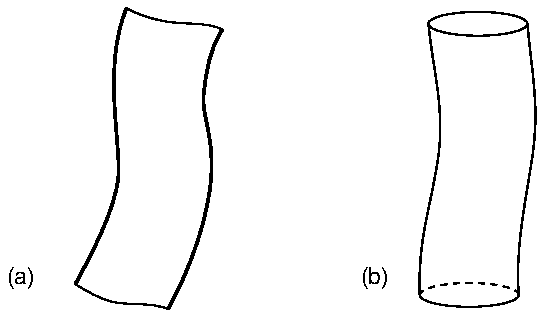
\includegraphics[width=0.82\linewidth]{figures/fig_3_1.pdf}
\caption{(a) 帯の位相を持つ開弦の世界面。太い曲線は弦の端点の世界線である。
(b) 円筒の位相を持つ閉弦の世界面。}
\label{fig:3.1}
\end{figure}

弦が相互作用する仕方はいくつも考えられる。
一つは、2本の弦が交差するときにエネルギーが生じる接触相互作用である。
もう一つは、何らかの量子場が媒介する長距離力である。
しかし、そのような相互作用を、対称性と整合するように弦理論に
\emph{付け加える}ことはできない。
なぜそうなのかについては、後である程度の理解を得ることになる。
許される相互作用は、世界面についての和にすでに暗黙に含まれているものだけである。
たとえば図\ref{fig:3.2}の世界面を考えよう。
図\ref{fig:3.2}(a)は、図\ref{fig:3.1}(a)の開弦振幅への量子補正のように見え、
2本の開弦からなる中間状態を含んでいる。
図\ref{fig:3.2}(b)には3本の外線の閉弦があり、1本の弦が2本に崩壊する過程を表している。
これこそが弦理論に相互作用を導入する正しい方法であることがわかる。
これらの相互作用が、有限でユニタリーであり、重力を含む整合的な理論を生み出すことを見るであろう。

\begin{figure}[tbp]
\centering
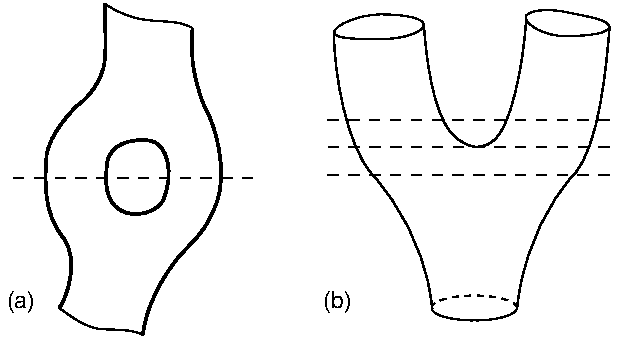
\includegraphics[width=0.86\linewidth]{figures/fig_3_2.pdf}
\caption{(a) 開弦の伝播への量子補正。(b) 1本の閉弦が2本に崩壊する過程。
破線は等時刻断面である。}
\label{fig:3.2}
\end{figure}

図\ref{fig:3.2}(b)の過程を、図\ref{fig:3.3}のように、
順々の時刻で観察してみると興味深い。
1本の閉弦が2本に分かれる。あるいは、その逆の過程では2本が1本につながる。
これが閉弦の基本的な相互作用である。
閉弦理論では、すべての粒子は弦のさまざまな励起状態として得られ、
すべての相互作用（たとえばゲージ相互作用、重力相互作用、Yukawa相互作用）は、
図\ref{fig:3.3}の一つの過程から生じる。
開弦を含む理論では、図\ref{fig:3.4}に示すように、
これに加えていくつかの過程が起こりうる。
ある時間分割を選ぶと、図\ref{fig:3.3}および図\ref{fig:3.4}の相互作用は
時空のある定まった点で起こるように見えるが、これは見かけにすぎない。
Lorentzブーストした座標系で別の時間分割を選ぶと、
見かけの相互作用は別の点に位置することになる。
時空に特別な点があるわけではない。
相互作用は世界面の大域的な位相だけから生じ、
世界面の局所的な性質は自由な場合と同じである。
序論で述べたように、このように相互作用が広がることによって、
重力の短距離発散が切り落とされる。

\begin{figure}[tbp]
\centering
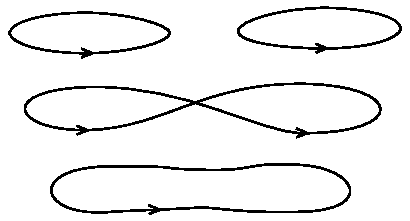
\includegraphics[width=0.67\linewidth]{figures/fig_3_3.pdf}
\caption{図\ref{fig:3.2}(b)の連続する等時刻断面。
矢印は弦の向きを表す。}
\label{fig:3.3}
\end{figure}

\begin{figure}[tbp]
\centering
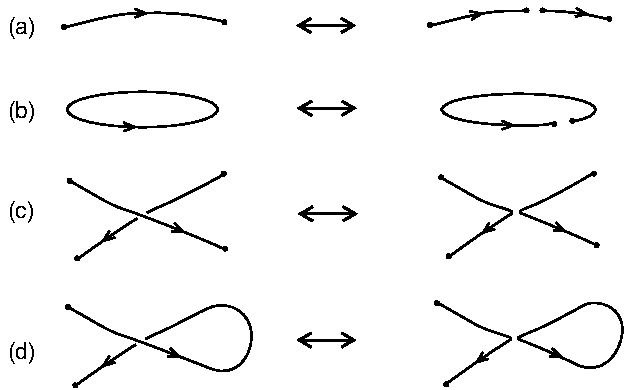
\includegraphics[width=0.84\linewidth]{figures/fig_3_4.pdf}
\caption{開弦を含む過程：
(a) 開弦$\leftrightarrow$開弦$+$開弦、
(b) 閉弦$\leftrightarrow$開弦、
(c) 開弦$+$開弦$\leftrightarrow$開弦$+$開弦、
(d) 開弦$\leftrightarrow$開弦$+$閉弦。}
\label{fig:3.4}
\end{figure}

実際には、世界面についての和にどの位相を含めるかによって、
いくつかの異なる弦理論が存在する。
まず、これまで描いてきた世界面には2種類の境界があることに注意しよう。
初期状態および終状態の弦の配位に対応する\emph{ソース境界}と、
開弦の端点の世界線に対応する\emph{端点境界}である。
ソース境界はひとまず無視しよう。
ソースの詳細については、この章の後のほうで議論する。
したがって、以下の議論で「境界」といえば端点境界を意味する。
すると、世界面についての和を定義する方法は次の4通りとなり、
これらは第1.4節の末尾に挙げた4種類の自由弦理論に対応する。
\begin{enumerate}
\item 向きのある閉弦：境界を持たない、向きのあるすべての世界面。
\item 向きのない閉弦：境界を持たないすべての世界面。
\item 向きのある閉弦と開弦：任意個数の境界を持つ、向きのあるすべての世界面。
\item 向きのない閉弦と開弦：任意個数の境界を持つすべての世界面。
\end{enumerate}

\begin{figure}[tbp]
\centering
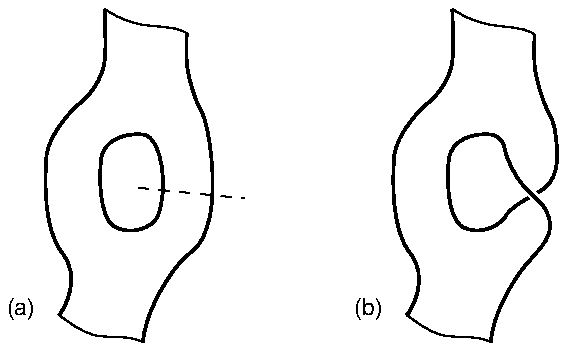
\includegraphics[width=0.80\linewidth]{figures/fig_3_5.pdf}
\caption{2本の開弦の振幅への、向きのある寄与(a)と向きのない寄与(b)。}
\label{fig:3.5}
\end{figure}

ここで、さらに説明すべきことが二つある。
第一は、向きのない世界面を含めることと、
第1.4節で説明した$\Omega=+1$への射影との関係である。
図\ref{fig:3.5}は、開弦を含む向きのない理論で和に含まれる二つの世界面を示している。
図\ref{fig:3.5}(b)の向きのない世界面は、
図\ref{fig:3.5}(a)の向きのある曲面を、$0\leq\sigma\leq\pi$で
パラメーター表示した破線に沿って切り、切り口上の場に
\begin{equation}
X^\mu_{\mathrm{upper}}(\sigma)
=X^\mu_{\mathrm{lower}}(\pi-\sigma)
\tag{3.1.2}\label{eq:3.1.2}
\end{equation}
を満たすことを要求するのと同等である。
これはさらに、開弦の状態に演算子$\Omega$を作用させることと同等である。
したがって、この二つの曲面を適切な重みで足し合わせることは、
$\Omega=+1$の状態へ射影する演算子$\frac12(1+\Omega)$を挿入することに相当する。
向きのある曲面と向きのない曲面のすべてについて和をとると、
すべての中間状態に射影演算子が挿入され、
スペクトルは$\Omega=+1$のセクターに制限される。

\begin{figure}[tbp]
\centering
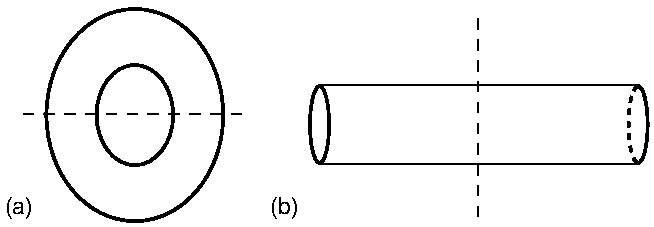
\includegraphics[width=0.90\linewidth]{figures/fig_3_6.pdf}
\caption{(a) 環帯：中間状態は2本の開弦からなる。
(b) 同じ位相を円筒として描いたもの：中間状態は1本の閉弦である。}
\label{fig:3.6}
\end{figure}

第二に、上の一覧には、開弦を持つが閉弦を持たない理論は含まれていない。
なぜそうなるのか、もう少し詳しく説明しよう。
図\ref{fig:3.6}(a)のように、環帯の位相を持つ世界面を考える。
便宜上、真空振幅だけを描いたが、
適切なソースをつなげれば同じ議論が散乱振幅にも適用できる。
破線からわかるように、これは2本の開弦からなる中間状態を持つ過程であり、
したがって、この位相の世界面は開弦を含むどの理論にも存在しなければならない。
図\ref{fig:3.6}(b)では、同じ位相を円筒として描き、
1本の閉弦からなる中間状態に沿って切り開いている。
したがって、開弦だけから出発したとしても、
世界面についての和には、開弦の散乱によって閉弦が生成される過程が必ず含まれる。
振幅を詳しく調べていく際に、これがどのように働くかを具体的に見ることになる。

開弦理論に閉弦が必要であることは、別の方法でも理解できる。
図\ref{fig:3.4}(a)、(b)の相互作用を、時間を逆にして考えよう。
それぞれ、2本の開弦が1本に結合する過程と、開弦から閉弦への遷移である。
相互作用点の近くでは、これらはどちらも二つの端点が合体する同じ過程である。
第二の相互作用を許さずに第一だけを許すには、
弦のダイナミクスに何らかの非局所的な制約を課す必要があるだろう。
これはきっと不整合になるはずである。
図\ref{fig:3.4}(c)、(d)についても同じ議論ができる。
そこでは、相互作用は局所的には一対の弦のつなぎ替えである。
したがって、開弦の相互作用を何か一つでも許せば、
開弦から閉弦を生成する過程も何かしら許されることになる。

\subsectionlink{Polyakov経路積分}\label{sec:3.2}

ここからは、Polyakovの形式の場について積分することで、
世界面についての和を具体的に組み立てていく。
第1章から一つ変更を加える。
Minkowski世界面計量$\gamma_{ab}$を、符号$(+,+)$の
Euclid世界面計量$g_{ab}(\sigma^1,\sigma^2)$で置き換えるのである。
積分は、すべてのEuclid計量と、
世界面のMinkowski時空へのすべての埋め込み$X^\mu(\sigma^1,\sigma^2)$にわたる。
\begin{equation}
\int[dX\,dg]\,\exp(-S).
\tag{3.2.1}\label{eq:3.2.1}
\end{equation}
Euclid作用は
\begin{equation}
S=S_X+\lambda\chi
\tag{3.2.2}\label{eq:3.2.2}
\end{equation}
であり、ここで
\begin{align}
S_X&=\frac{1}{4\pi\alpha'}\int_M d^2\sigma\,g^{1/2}g^{ab}
       \partial_aX^\mu\partial_bX_\mu,
\tag{3.2.3a}\label{eq:3.2.3a}\\
\chi&=\frac{1}{4\pi}\int_M d^2\sigma\,g^{1/2}R
       +\frac{1}{2\pi}\int_{\partial M}ds\,k.
\tag{3.2.3b}\label{eq:3.2.3b}
\end{align}
測地曲率$k$は演習1.3で定義した。
ここでは境界がつねに空間的であることに注意しよう。

Euclid経路積分の利点は、計量についての積分がより明確に定義されることにある。
これまで説明してきた位相的に非自明な世界面は、
非特異なEuclid計量を持ちうるが、非特異なMinkowski計量を持つことはできない。
本書ではEuclid理論\eqref{eq:3.2.1}を出発点とし、
それに厳密な定義を与える方法と、それがこれまで述べてきた性質を備える
整合的な時空の理論を定義することを示す。
しかし、その前に、これが最初に出発したMinkowski理論と等価であることを、
簡単な形式的議論によって示しておこう。

再び点粒子の例から始める。この場合、経路積分
\begin{equation}
\int[d\eta\,dX]\,
\exp\left[\frac{i}{2}\int d\tau
\left(\eta^{-1}\dot X^\mu\dot X_\mu-\eta m^2\right)\right]
\tag{3.2.4}\label{eq:3.2.4}
\end{equation}
は振動的である。
$\eta$と$X^\mu$についての経路積分は通常の積分の積であるから、
通常の積分と同様に積分路を変形することができる。
無限小の$\theta$に対して
\begin{equation}
\eta(\tau)\longrightarrow e^{-i\theta}\eta(\tau),\qquad
X^0(\tau)\longrightarrow e^{-i\theta}X^0(\tau)
\tag{3.2.5}\label{eq:3.2.5}
\end{equation}
とすると、指数の中のすべての項に負の実部が加わるため、
これは収束因子として働く。
そこで、場の空間で積分路の回転を行い、
$\eta=-ie$、$X^0=-iX^D$まで回すことができる。
積分は
\begin{equation}
\int[de\,dX]\,
\exp\left[-\frac12\int d\tau
\left(e^{-1}\sum_{\mu=1}^{D}\dot X^\mu\dot X^\mu+em^2\right)\right]
\tag{3.2.6}\label{eq:3.2.6}
\end{equation}
となる。
これは経路積分\eqref{eq:3.2.1}に対応する、Euclid点粒子の場合の式である。
行ったのは積分路の回転だけなので、Euclid経路積分はMinkowski経路積分と
同じ振幅を与える。

Polyakov作用についても、計量を四脚場を用いて
$\gamma_{ab}=-e_a^0e_b^0+e_a^1e_b^1$と書き、
$e_a^0$に対して同じ回転を行えば、同じ手順が使える。
これによって、Minkowski経路積分とEuclid経路積分の等価性が形式的に正当化される。
\footnote[1]{2次元より高い次元では、Hilbert作用が回転のもとで
より複雑に振る舞うため、事情はそれほど簡単ではない。
経路積分を減衰させる単純な回転は存在しない。
特に、4次元重力のEuclid経路積分が何を意味するかは、非常に不確かである。}
両者をそれぞれ光円錐ゲージと共形ゲージで扱うと同じ振幅が定義されることが、
具体的な計算によって示されている。
作用\eqref{eq:3.2.3a}では、時空がMinkowski的であることを強調するために、
前章と同様、$X^0$の回転を暗黙のままにしておいた。
$X^0$を用いて書けば、運動方程式とOPEは計量$\eta^{\mu\nu}$に関して共変である。

$\chi$が2次元では局所的に全微分であり、
そのため世界面の位相だけに依存することは、すでに述べた。
これは世界面の\emph{Euler数}である。
したがって、経路積分における$e^{-\lambda\chi}$という因子は、
世界面についての和の中で、異なる位相の相対的な重みだけに影響する。
特に、図\ref{fig:3.1}(a)から図\ref{fig:3.2}(a)へ移る際に行ったように、
世界面に帯を一つ付け加えると、Euler数が1だけ減少し、
経路積分には$e^\lambda$という重みの因子が余分に掛かる。
帯を加えることは仮想的な開弦の放出と再吸収に対応するので、
どの過程からであっても、開弦を放出する振幅は$e^{\lambda/2}$に比例する。
任意の世界面に取っ手を一つ付け加えると、
Euler数が2だけ減少し、$e^{2\lambda}$という因子が掛かる。
これは閉弦の放出と再吸収に対応するので、
閉弦を放出する振幅は$e^\lambda$に比例する。
したがって、作用のEuler項が弦理論の結合定数を制御し、
\begin{equation}
g_{\mathrm o}^{\,2}\sim g_{\mathrm c}\sim e^\lambda
\tag{3.2.7}\label{eq:3.2.7}
\end{equation}
となる。
ところで、$\lambda$は理論の自由なパラメーターのように見えるかもしれない。
すると、弦理論にはそのようなパラメーターが存在しないという序論の主張と矛盾する。
これは重要な点であり、第3.7節で解決する。

余談になるが、結合定数の数え上げは、
弦のソースを持つ世界面にも単純な形で拡張できる。
閉弦のソースは閉じた境界ループであり、開弦のソースは境界の一部分である。
便宜上、開弦のソース境界が世界面計量に関して直角に端点境界と交わることを要求する。
角では境界曲率$k$が発散するので注意しなければならない。
Euler数は
\begin{equation}
\chi=\tilde\chi+\frac14n_{\mathrm c}
\tag{3.2.8}\label{eq:3.2.8}
\end{equation}
である。ここで、$\tilde\chi$には境界の滑らかな部分に沿った積分だけを含め、
$n_{\mathrm c}$は角の個数を表す。
経路積分に対する正しい重みは
\begin{equation}
\exp(-\lambda\tilde\chi)=\exp(-\lambda\chi+\lambda n_{\mathrm c}/4)
\tag{3.2.9}\label{eq:3.2.9}
\end{equation}
である。
これはユニタリティから従う。
世界面を切って内部線を減らし、外部ソースを増やしても、
$\lambda$依存性は変わってはならない。
$\tilde\chi$に含まれる表面積分が切り口で相殺するため、
重み\eqref{eq:3.2.9}ならばこの条件が満たされる。
閉弦のソースを加えることは世界面に穴を開けることに相当し、
$\chi$を1だけ減少させる。
開弦のソースを加えても$\chi$は変わらず、$n_{\mathrm c}$が2だけ増加する。
したがって、閉弦または開弦を放出する振幅について、
同じ結論\eqref{eq:3.2.7}に到達する。

\subsectionlink{ゲージ固定}\label{sec:3.3}

経路積分\eqref{eq:3.2.1}は、完全には正しくない。
そこには膨大な重複計数が含まれている。
局所的な$\mathrm{diff}\times\mathrm{Weyl}$対称性によって互いに関係する
配位$(X,g)$と$(X',g')$は、同じ物理的配位を表すからである。
実質的には、この局所対称群の体積で割る必要がある。
\begin{equation}
\int\frac{[dX\,dg]}{V_{\mathrm{diff}\times\mathrm{Weyl}}}\,\exp(-S)
\equiv Z.
\tag{3.3.1}\label{eq:3.3.1}
\end{equation}
これをゲージ固定によって行う。
すなわち、各ゲージ同値類を1回ずつ横切る断面に沿って積分し、
その断面上の正しい測度をFaddeev--Popov法によって求める。

第1章では光円錐ゲージを課した。
これはある目的には有用だが、理論の対称性の一部を隠してしまうので、
ここでは別の選び方をする。
計量は対称なので三つの独立な成分を持つこと、
そして、二つの座標と計量の局所的なスケールという、
三つのゲージ関数があることに注意しよう。
したがって、計量についての積分を消去し、
ある特定の関数形に固定するのにちょうど十分なゲージ自由度がある。
この固定した計量を\emph{基準計量}と呼び、
\begin{equation}
g_{ab}(\sigma)\longrightarrow\hat g_{ab}(\sigma)
\tag{3.3.2}\label{eq:3.3.2}
\end{equation}
と書く。
単純な選択は、平坦な計量、すなわち\emph{単位ゲージ}の計量
\begin{equation}
\hat g_{ab}(\sigma)=\delta_{ab}
\tag{3.3.3}\label{eq:3.3.3}
\end{equation}
である。
場合によっては、$\mathrm{diff}$群だけの効果を考えたいこともある。
その場合、任意の計量を、単位計量とWeyl変換だけ異なる形にすることができる。
これが\emph{共形ゲージ}である。
\begin{equation}
\hat g_{ab}(\sigma)=\exp[2\omega(\sigma)]\delta_{ab}.
\tag{3.3.4}\label{eq:3.3.4}
\end{equation}

場とゲージ対称性のこの数え上げが実際にうまくいくこと、
つまり、任意の計量を、少なくとも局所的に、
世界面上のある近傍では平坦な形にできることを具体的に見よう。
まずWeyl変換を行い、$g_{ab}$から作られるRicciスカラーをゼロにする。
RicciスカラーのWeyl変換は
\begin{equation}
g'^{\,1/2}R'=g^{1/2}(R-2\nabla^2\omega)
\tag{3.3.5}\label{eq:3.3.5}
\end{equation}
である。
$R'=0$とするには、$2\nabla^2\omega=R$を$\omega$に関する方程式として解く必要がある。
静電気学の標準的な議論により、これは少なくとも局所的にはつねに可能である。
さて、2次元ではRicciスカラーがゼロになることは、
Riemannテンソル全体がゼロになることを意味する。
Riemannテンソルの対称性から
\begin{equation}
R_{abcd}=\frac12(g_{ac}g_{bd}-g_{ad}g_{bc})R
\tag{3.3.6}\label{eq:3.3.6}
\end{equation}
が従うからである。
したがって、計量は平坦であり、座標変換によって単位計量\eqref{eq:3.3.3}と同等になる。

実際には、局所的には少し余分なゲージ自由度が残っている。
計量を単位ゲージのままに保つ$\mathrm{diff}\times\mathrm{Weyl}$変換が存在し、
これは計量の選択によっては固定されない。
ここでは、第2章と同じく複素座標$z=\sigma^1+i\sigma^2$を導入すると便利である。
この座標では平坦な計量は$ds^2=dz\,d\bar z$となる。
$z'$が$z$の正則関数となる座標変換
\begin{equation}
z'\equiv\sigma'^{\,1}+i\sigma'^{\,2}=f(z)
\tag{3.3.7}\label{eq:3.3.7}
\end{equation}
と、Weyl変換とを組み合わせて考える。
新しい計量は
\begin{equation}
ds'^{\,2}=\exp(2\omega)|\partial_zf|^{-2}\,dz'\,d\bar z'
\tag{3.3.8}\label{eq:3.3.8}
\end{equation}
である。
したがって、
\begin{equation}
\omega=\ln|\partial_zf|
\tag{3.3.9}\label{eq:3.3.9}
\end{equation}
ならば計量は不変である。
この余分なゲージ自由度は、先ほどの数え上げ（$3=3$）とは矛盾しない。
その食い違いに当たる正則な再パラメーター化の集合は、
すべての再パラメーター化の集合に比べれば測度ゼロだからである。

世界面全体を考えると、この余分な自由度のほとんど、またはすべては境界条件によって取り除かれる。
ここには二つの論点がある。
第一に、Noetherの定理とWard恒等式を議論した際、
式\eqref{eq:2.3.10}の下で、これらの結果は、
対称性が世界面上で局所的に定義されることだけに依存すると注意深く強調した。
したがって、変換\eqref{eq:3.3.7}、\eqref{eq:3.3.9}は、
保存カレントとWard恒等式をもたらす。
これは、まさに第2章で研究した共形不変性である。
それが、単位計量を不変に保つ$\mathrm{diff}\times\mathrm{Weyl}$の部分群として
現れることがわかる。

第二の論点は、世界面全体を考えたとき、
計量とゲージの自由度の数え上げがどうなるかである。
これは第5章で取り上げる。
そこで、大域的には両者の間に、有限個のパラメーターという小さな食い違いがあることを見る。
それまでは、世界面理論の局所的性質だけを扱うことにする。

\subsubsectionlink*{Faddeev--Popov行列式}

計量を固定すると、汎関数積分は$X^\mu$だけでパラメーター表示される断面に沿ったものとなる。
正しい測度を得るために、Faddeev--Popovの手順に従う。
手順は、Yang--Mills理論でゲージ固定された測度を得るために用いるものと同じだが、
ここでは自己完結した説明を与える。
図\ref{fig:3.7}に示すその考え方は、
経路積分をゲージ群についての積分とゲージ断面に沿った積分との積に分離し、
前者で割るというものである。
Faddeev--Popov行列式は、この変数変換のJacobianである。

\begin{figure}[tbp]
\centering
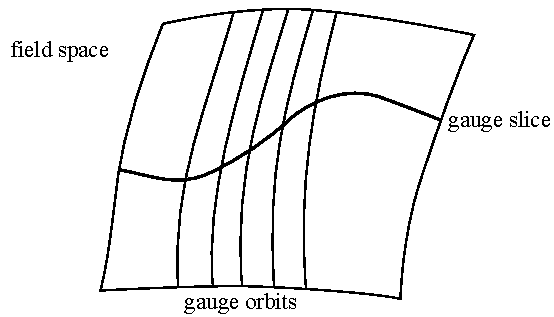
\includegraphics[width=0.84\linewidth]{figures/fig_3_7.pdf}
\caption{Faddeev--Popovの手順の模式図。
ゲージ軌道は、ゲージ同値な配位からなる族である。
場の空間全体について積分して軌道の体積で割ることは、
各軌道と1回ずつ交わる断面について、適切なJacobianを伴って積分することと同等である。
図中のfield spaceは場の空間、gauge sliceはゲージ断面、
gauge orbitsはゲージ軌道を表す。}
\label{fig:3.7}
\end{figure}

座標変換とWeyl変換を組み合わせた変換を、略して$\zeta$と書こう。
\begin{equation}
\zeta:g\longrightarrow g^\zeta,\qquad
g^\zeta_{ab}(\sigma')
=\exp[2\omega(\sigma)]
\frac{\partial\sigma^c}{\partial\sigma'^{\,a}}
\frac{\partial\sigma^d}{\partial\sigma'^{\,b}}g_{cd}(\sigma).
\tag{3.3.10}\label{eq:3.3.10}
\end{equation}
標準的な道筋に従い、Faddeev--Popov測度$\Delta_{\mathrm{FP}}$を
\begin{equation}
1=\Delta_{\mathrm{FP}}(g)\int[d\zeta]\,\delta(g-\hat g^\zeta)
\tag{3.3.11}\label{eq:3.3.11}
\end{equation}
によって定義する。ここでも$\hat g_{ab}$は基準計量である。
式\eqref{eq:3.3.11}の$[d\zeta]$は、
$\mathrm{diff}\times\mathrm{Weyl}$群上のゲージ不変な測度である。
この測度の具体的な形は必要にならない。
その存在の問題については次節で議論する。
デルタ関数は実際にはデルタ汎関数であり、
各点で$g_{ab}(\sigma)=\hat g^\zeta_{ab}(\sigma)$であることを要求している。

\eqref{eq:3.3.11}を汎関数積分\eqref{eq:3.3.1}に挿入すると、
後者は
\begin{equation}
Z[\hat g]
=\int\frac{[d\zeta\,dX\,dg]}{V_{\mathrm{diff}\times\mathrm{Weyl}}}
\Delta_{\mathrm{FP}}(g)\delta(g-\hat g^\zeta)\exp(-S[X,g])
\tag{3.3.12}\label{eq:3.3.12}
\end{equation}
となる。
後で参照するために、基準計量の選択に対する$Z$の依存性を明示しておく。
$g_{ab}$について積分を実行し、さらに積分変数の名前を$X\to X^\zeta$と変えると、
\begin{equation}
Z[\hat g]
=\int\frac{[d\zeta\,dX^\zeta]}{V_{\mathrm{diff}\times\mathrm{Weyl}}}
\Delta_{\mathrm{FP}}(\hat g^\zeta)\exp(-S[X^\zeta,\hat g^\zeta])
\tag{3.3.13}\label{eq:3.3.13}
\end{equation}
を得る。
ここで、$\Delta_{\mathrm{FP}}$、汎関数積分の測度$[dX]$、
作用のゲージ不変性を用いると、\footnote[2]{この不変性は次のように示せる。
\[
\begin{aligned}
\Delta_{\mathrm{FP}}(g^\zeta)^{-1}
&=\int[d\zeta']\,\delta(g^\zeta-\hat g^{\zeta'})\\
&=\int[d\zeta']\,\delta(g-\hat g^{\zeta^{-1}\cdot\zeta'})\\
&=\int[d\zeta'']\,\delta(g-\hat g^{\zeta''})
=\Delta_{\mathrm{FP}}(g)^{-1}.
\end{aligned}
\]
ここで$\zeta''=\zeta^{-1}\cdot\zeta'$である。
第2の等号ではデルタ関数のゲージ不変性を、
第3の等号では測度の不変性を用いた。}
\begin{equation}
Z[\hat g]
=\int\frac{[d\zeta\,dX]}{V_{\mathrm{diff}\times\mathrm{Weyl}}}
\Delta_{\mathrm{FP}}(\hat g)\exp(-S[X,\hat g])
\tag{3.3.14}\label{eq:3.3.14}
\end{equation}
となる。
最後に、被積分関数には$\zeta$に依存するものが何もないので、
$\zeta$についての積分は単にゲージ群の体積を与え、分母を打ち消す。
したがって、
\begin{equation}
Z[\hat g]=\int[dX]\,\Delta_{\mathrm{FP}}(\hat g)\exp(-S[X,\hat g])
\tag{3.3.15}\label{eq:3.3.15}
\end{equation}
が残る。このように、$\Delta_{\mathrm{FP}}(\hat g)$は断面上の正しい測度である。

Faddeev--Popov測度の表式\eqref{eq:3.3.11}を評価するために、
ゲージの選択がゲージ対称性をちょうど完全に固定すると仮定してみよう。
すなわち、デルタ関数$\delta(g-\hat g^\zeta)$がゼロでないのは、
厳密に一つの$\zeta$に対してだけであるとする。
$\delta(\hat g-\hat g^\zeta)$の場合には、それは恒等変換である。
上で述べたように、大域的には小さな食い違いがあるが、
それは必要になったときに扱うことにする。
世界面の局所的性質には影響しないからである。
$\zeta$が恒等変換に近いとき、
\begin{equation}
\begin{aligned}
\delta g_{ab}
&=2\delta\omega\,g_{ab}-\nabla_a\delta\sigma_b-\nabla_b\delta\sigma_a\\
&=(2\delta\omega-\nabla_c\delta\sigma^c)g_{ab}
   -2(P_1\delta\sigma)_{ab}
\end{aligned}
\tag{3.3.16}\label{eq:3.3.16}
\end{equation}
と展開できる。
ここでは、ベクトルをトレースのない対称2階テンソルへ写す微分演算子$P_1$を
\begin{equation}
(P_1\delta\sigma)_{ab}
=\frac12\left(\nabla_a\delta\sigma_b+\nabla_b\delta\sigma_a
             -g_{ab}\nabla_c\delta\sigma^c\right)
\tag{3.3.17}\label{eq:3.3.17}
\end{equation}
と定義した。
恒等変換の近傍では、逆行列式\eqref{eq:3.3.11}は
\begin{equation}
\begin{aligned}
&\Delta_{\mathrm{FP}}(\hat g)^{-1}\\
&\quad=\int[d\delta\omega\,d\delta\sigma]\,
 \delta\left[-(2\delta\omega-\hat\nabla\cdot\delta\sigma)\hat g
                    +2\hat P_1\delta\sigma\right]\\
&\quad=\int[d\delta\omega\,d\beta\,d\delta\sigma]\,
 \exp\biggl\{2\pi i\int d^2\sigma\,\hat g^{1/2}\beta^{ab}\\
&\hspace{37mm}\times
 \left[-(2\delta\omega-\hat\nabla\cdot\delta\sigma)\hat g
                    +2\hat P_1\delta\sigma\right]_{ab}\biggr\}\\
&\quad=\int[d\beta'\,d\delta\sigma]\,
 \exp\left\{4\pi i\int d^2\sigma\,\hat g^{1/2}
                 \beta'^{\,ab}(\hat P_1\delta\sigma)_{ab}\right\}
\end{aligned}
\tag{3.3.18}\label{eq:3.3.18}
\end{equation}
となる。
微分演算子の上のハットは、その演算子が基準計量$\hat g$を含むことを表す。
第2の等号では、デルタ汎関数の積分表示を用い、
対称テンソル場$\beta^{ab}$を導入した。
第3の等号では、$\delta\omega$について積分した。
すると、$\beta^{ab}$のトレースがゼロであることを強制するデルタ汎関数が生じる。
したがって、汎関数積分$[d\beta']$は、
トレースのない対称テンソルについての積分となる。
これで、$\Delta_{\mathrm{FP}}(\hat g)^{-1}$を、
ベクトル場$\delta\sigma^a$およびトレースのない対称テンソル$\beta'^{\,ab}$に
関する汎関数積分として表すことができた。

付録で説明するように、各ボソン場を対応するGrassmannゴースト場に置き換えると、
この経路積分の逆数を得ることができる。
\begin{align}
\delta\sigma^a&\longrightarrow c^a,
\tag{3.3.19a}\label{eq:3.3.19a}\\
\beta'_{ab}&\longrightarrow b_{ab}.
\tag{3.3.19b}\label{eq:3.3.19b}
\end{align}
$b^{ab}$は$\beta'^{\,ab}$と同様、トレースを持たない。
したがって、
\begin{equation}
\Delta_{\mathrm{FP}}(\hat g)=\int[db\,dc]\,\exp(-S_{\mathrm g})
\tag{3.3.20}\label{eq:3.3.20}
\end{equation}
となる。ここで、場に便利な規格化を選ぶと、ゴースト作用$S_{\mathrm g}$は
\begin{equation}
S_{\mathrm g}
=\frac{1}{2\pi}\int d^2\sigma\,\hat g^{1/2}b_{ab}\hat\nabla^{a}c^{b}
=\frac{1}{2\pi}\int d^2\sigma\,\hat g^{1/2}b_{ab}(\hat P_1c)^{ab}
\tag{3.3.21}\label{eq:3.3.21}
\end{equation}
である。
世界面上で局所的には、Polyakov経路積分はここで
\begin{equation}
Z[\hat g]=\int[dX\,db\,dc]\,\exp(-S_X-S_{\mathrm g})
\tag{3.3.22}\label{eq:3.3.22}
\end{equation}
となった。
作用は場の2次式なので、付録で説明するように、
経路積分を行列式を用いて評価することができる。
この段階の計算は第5章でより詳しく行うが、ここでの結果は
\begin{equation}
Z[\hat g]=(\det\hat\nabla^2)^{-D/2}\det\hat P_1
\tag{3.3.23}\label{eq:3.3.23}
\end{equation}
である。
第一の行列式は$X$についての積分から、
第二の行列式はゴーストについての積分から生じる。

共形ゲージ$\hat g_{ab}(\sigma)=\exp[2\omega(\sigma)]\delta_{ab}$では、
ゴースト作用\eqref{eq:3.3.21}は
\begin{equation}
\begin{aligned}
S_{\mathrm g}
&=\frac{1}{2\pi}\int d^2z\,
  \left(b_{zz}\nabla_{\bar z}c^z+b_{\bar z\bar z}\nabla_zc^{\bar z}\right)\\
&=\frac{1}{2\pi}\int d^2z\,
  \left(b_{zz}\partial_{\bar z}c^z+b_{\bar z\bar z}\partial_zc^{\bar z}\right)
\end{aligned}
\tag{3.3.24}\label{eq:3.3.24}
\end{equation}
となる。
最終的な形に$\omega(\sigma)$が現れないことに注意しよう。
これは、$z$添字だけを持つテンソルの$\bar z$方向の共変微分が
単純な偏微分に帰着し、逆の場合も同様だからである。
読者は接続テンソルを計算すればこれを確認できる。
この性質を利用するために、$b$には下付き、$c$には上付きの添字を用いた。
作用\eqref{eq:3.3.24}はWeyl不変なので、
$b_{ab}$と$c^a$はWeyl変換のもとで中性でなければならない。
これは、たとえば余分な計量因子を含む$b^{ab}$や$c_a$とは対照的である。
共形変換は座標変換\eqref{eq:3.3.7}とWeyl変換\eqref{eq:3.3.9}の組み合わせなので、
$b_{ab}$と$c^a$の共形変換は、テンソル添字から直ちに読み取ることができる。
これは$(h_b,h_c)=(2,-1)$の$bc$共形場理論と、
$(\tilde h_b,\tilde h_c)=(2,-1)$の$\tilde b\tilde c$共形場理論である。

ここで示した、ゲージ固定された経路積分の導出は、
「発見的な」導出と呼ばれることがある。
問題は、出発点であるPolyakov汎関数積分\eqref{eq:3.3.1}が、
膨大なゲージの重複計数のために明確に定義されていないことである。
一方、ゲージ固定された汎関数積分\eqref{eq:3.3.22}はきちんと定義されており、
具体的に計算できる。
実用上は、ゲージ固定された形を真の出発点と見なし、
ゲージ不変な形は直観的な解釈を与えるものと考えるべきなのかもしれない。
ゲージ固定された形にも、ゲージ対称性の本質的な内容は
\emph{BRST不変性}としてなお残っている。これは次章で取り上げる。

開弦の場合には、境界の一部分を含むパッチも考える必要がある。
汎関数積分は、固定された座標領域上の場についての積分と考えると便利なので、
$\mathrm{diff}$不変性は、境界をそれ自身に写す座標変換に制限される。
したがって、変分$\delta\sigma^a$の法線成分はゼロとなる。
\begin{equation}
n_a\delta\sigma^a=0.
\tag{3.3.25}\label{eq:3.3.25}
\end{equation}
この境界条件は対応するゴースト場にも引き継がれる。
\begin{equation}
n_ac^a=0.
\tag{3.3.26}\label{eq:3.3.26}
\end{equation}
したがって、$c^a$は接ベクトル$t^a$に比例する。
続いて、運動方程式から$b_{ab}$の境界条件が得られる。
そこには表面項
\begin{equation}
\int_{\partial M}ds\,n^ab_{ab}\delta c^b=0
\tag{3.3.27}\label{eq:3.3.27}
\end{equation}
が現れる。
$c^a$の境界条件と合わせると、これは
\begin{equation}
n_at_bb^{ab}=0
\tag{3.3.28}\label{eq:3.3.28}
\end{equation}
を意味する。
これらは、第2.7節で用いた境界条件である。

% 原文PDF112--123頁（本文90--101頁）、3.4--3.5。
\subsectionlink{Weyl 異常}\label{sec:3.4}

弦理論の重要な特徴は、すべての時空背景で整合的なのではなく、ある条件を満たす背景でのみ整合的であるという点である。平坦な時空におけるボソン弦理論では、その条件は $D=26$ である。これは最初、散乱振幅の病的な振る舞いとして発見された。光円錐による解析では、1.3節で手短に、かなり直観的に説明したように、Lorentz 不変性の喪失として現れる。この制限の根本的な原因は、世界面の局所対称性における異常である。現在の形式では、その異常は Weyl 対称性にある。$T^a{}_a$ は古典的にはゼロだが、量子論ではそうではない。

場の量子論を学んだ読者は、同じ言葉では説明されなかったかもしれないが、すでに関連する異常に出会っている。大域的な Weyl 変換、すなわち $\omega(\sigma)=\text{定数}$ は、長さ全体のスケール変換と等価である。四次元における、よく知られたいくつかの場の理論は、そのようなスケール変換の下で古典的に不変である。これには、$\phi^4$ 相互作用をもつ質量のないスカラー場の理論や、非 Abel ゲージ理論が含まれる。Lagrangian に次元をもつパラメータが含まれず、どの場合も結合定数は無次元なので、スケール不変性は明らかである。しかし、量子論の発散により、それぞれの理論にゼロでない繰り込み群のベータ関数があることを、われわれは知っている。これは、有効結合定数が実際には長さの尺度の関数であることを意味する。対応して、エネルギー運動量テンソルのトレースは古典論ではゼロであるが、量子効果を考慮するとゼロでなくなり、ベータ関数に比例する。

前節では、異常の可能性を無視した。この点を確かめる必要がある。ゲージ固定した経路積分 $Z[g]$ は、本当に基準計量の選択に依存しないのだろうか。
\begin{equation}
Z[g^\zeta]=Z[g]\;?
\tag{3.4.1}\label{eq:3.4.1}
\end{equation}
4.2節では、これをより一般的なゲージの変更へ拡張する。便宜上、以下では $g$ のハットを省く。また、追加の挿入を含む経路積分
\begin{equation}
\langle\cdots\rangle_g
\equiv\int[dX\,db\,dc]\,\exp\bigl(-S[X,b,c,g]\bigr)\cdots
\tag{3.4.2}\label{eq:3.4.2}
\end{equation}
にも関心がある。その場合には、
\begin{equation}
\langle\cdots\rangle_{g^\zeta}=\langle\cdots\rangle_g
\tag{3.4.3}\label{eq:3.4.3}
\end{equation}
も要求する。現時点では、挿入そのものの詳細には関心がない。それは次の二つの節の主題となる。そこで、「$\cdots$」に含まれる場の位置の近傍でゼロとなるゲージ変換 $\zeta$ に注意を限る。つまり、演算子方程式として Weyl 不変性が成り立つことを要求している。

量子論で微分同相不変性と Poincaré 不変性を保つのは容易である。たとえば、A.1節で調和振動子について行ったように、Pauli--Villars レギュレータを用い、質量をもつレギュレータ場の経路積分で割ることによって、ゲージ固定した経路積分を定義できる。質量をもつレギュレータ場は、微分同相不変かつ Poincaré 不変な仕方で計量に結合できる。しかし、レギュレータ場 $Y^\mu$ の、微分同相不変かつ Poincaré 不変な質量項 $\mu^2\int d^2\sigma\,g^{1/2}Y^\mu Y_\mu$ は、Weyl 不変ではない。したがって、Weyl 不変性は直接確かめねばならない。Weyl 変換に対して不変性\hyperref[eq:3.4.3]{(3.4.3)}は成り立つだろうか。任意の Weyl 変換は、無限小変換を繰り返した結果として得られるため、後者を調べれば十分である。

エネルギー運動量テンソル $T^{ab}$ は、計量に関する経路積分の無限小変分である。
\begin{equation}
\delta\langle\cdots\rangle_g
=-\frac1{4\pi}\int d^2\sigma\,g(\sigma)^{1/2}
\delta g_{ab}(\sigma)\left\langle T^{ab}(\sigma)\cdots\right\rangle_g.
\tag{3.4.4}\label{eq:3.4.4}
\end{equation}
古典的には、$T^{ab}$ はすべて作用の変分から生じ、これは Noether の定義
\begin{equation}
T^{ab}(\sigma)\overset{\text{古典的}}{=}
\frac{4\pi}{g(\sigma)^{1/2}}
\frac{\delta}{\delta g_{ab}(\sigma)}S
\tag{3.4.5}\label{eq:3.4.5}
\end{equation}
と一致する。また、平坦な世界面の極限では、それまでの定義に帰着する。$\delta g_{ab}$ を座標変換の形にとれば、経路積分の微分同相不変性は $T^{ab}$ の保存を意味する。

以下の解析では、まず境界項の可能性を無視する。Weyl 変換に対して、$T^{ab}$ の定義\hyperref[eq:3.4.4]{(3.4.4)}は
\begin{equation}
\delta_{\mathrm W}\langle\cdots\rangle_g
=-\frac1{2\pi}\int d^2\sigma\,g(\sigma)^{1/2}
\delta\omega(\sigma)\left\langle T^a{}_a(\sigma)\cdots\right\rangle_g
\tag{3.4.6}\label{eq:3.4.6}
\end{equation}
を意味する。したがって、一般の挿入「$\cdots$」を含む場合の Weyl 不変性は、エネルギー運動量テンソルのトレースがゼロであるという演算子としての主張に言い換えられる。
\begin{equation}
T^a{}_a\overset{?}{=}0.
\tag{3.4.7}\label{eq:3.4.7}
\end{equation}
古典作用は Weyl 不変であるが、完全にゲージ不変なレギュレータを見いだせていないため、量子論ではトレースがゼロでないかもしれない。微分同相不変性と Poincaré 不変性は保っているので、トレースはそれらに対して不変でなければならない。また、平坦な場合の理論が共形不変であることを前章から知っているので、平坦な場合にはゼロにならねばならない。すると可能性は一つしか残らない。
\begin{equation}
T^a{}_a=a_1R.
\tag{3.4.8}\label{eq:3.4.8}
\end{equation}
ここで $a_1$ はある定数であり、$R$ はやはり世界面の Ricci スカラーである。二つを超える微分を含む項は、次元の理由から禁じられる。世界面の長さを単位として測ると、$g_{ab}$ と $X^\mu$ はともに無次元なので、式\hyperref[eq:3.4.8]{(3.4.8)}の定数 $a_1$ も無次元である。より多くの微分を含む項の係数は、経路積分の定義に用いたカットオフ長さの正のべきを含むことになる。したがって、カットオフをゼロにする極限で、そのような項は消える。

\subsubsection*{Weyl 異常の計算}

ゲージ不変な理論を妨げうるものは、一つの数 $a_1$ に帰着した。実際、この数は、すでに計算した量、すなわち平坦な世界面上の CFT の中心電荷 $c$ に比例する。$a_1$ と $c$ はどちらも、成分は異なるものの、エネルギー運動量テンソルの二点関数に関係している。両者の正確な関係を得るには、次のように微分同相不変性を用いる必要がある。

共形ゲージでは、
\begin{equation}
T_{z\bar z}=\frac{a_1}2g_{z\bar z}R.
\tag{3.4.9}\label{eq:3.4.9}
\end{equation}
共変微分をとると、
\begin{equation}
\nabla^{\bar z}T_{\bar z z}
=\frac{a_1}2\nabla^{\bar z}(g_{z\bar z}R)
=\frac{a_1}2\partial_zR.
\tag{3.4.10}\label{eq:3.4.10}
\end{equation}
ここでは、計量が共変的に一定であることを用いた。すると、$T_{ab}$ の保存則から、
\begin{equation}
\nabla^zT_{zz}=-\nabla^{\bar z}T_{\bar z z}
=-\frac{a_1}2\partial_zR.
\tag{3.4.11}\label{eq:3.4.11}
\end{equation}
$a_1$ を決めるため、左辺と右辺の Weyl 変換を比較する。右辺の Weyl 変換(3.3.5)は
\begin{equation}
a_1\partial_z\nabla^2\delta\omega
\approx4a_1\partial_z^2\partial_{\bar z}\delta\omega
\tag{3.4.12}\label{eq:3.4.12}
\end{equation}
である。ここでは、平坦な世界面の周りで展開した。$T_{zz}$ の Weyl 変換を得るには、まず共形変換\hyperref[eq:2.4.24]{(2.4.24)}を用いる。
\begin{equation}
\epsilon^{-1}\delta T_{zz}(z)
=-\frac c{12}\partial_z^3v^z(z)
-2\partial_zv^z(z)T_{zz}(z)-v^z(z)\partial_zT_{zz}(z).
\tag{3.4.13}\label{eq:3.4.13}
\end{equation}
3.3節の議論によると、この共形変換は座標変換 $\delta z=\epsilon v$ と、Weyl 変換 $2\delta\omega=\epsilon\partial v+\epsilon(\partial v)^*$ からなる。変分の最後の二項はテンソルの座標変換である。したがって、平坦な空間の周りの最低次における Weyl 変換は
\begin{equation}
\delta_{\mathrm W}T_{zz}=-\frac c6\partial_z^2\delta\omega
\tag{3.4.14}\label{eq:3.4.14}
\end{equation}
である。$\partial^z=2\partial_{\bar z}$ を作用させ、変換\hyperref[eq:3.4.12]{(3.4.12)}と比較すると、
\begin{equation}
c=-12a_1,\qquad T^a{}_a=-\frac c{12}R
\tag{3.4.15}\label{eq:3.4.15}
\end{equation}
を得る。

これを、少し長い別の道筋でもう一度導こう。その途中で、有用な中間結果が得られる。共形ゲージでは、
\begin{align}
R&=-2\exp(-2\omega)\partial_a\partial_a\omega,
\tag{3.4.16a}\label{eq:3.4.16a}\\
\nabla^2&=\exp(-2\omega)\partial_a\partial_a.
\tag{3.4.16b}\label{eq:3.4.16b}
\end{align}
二つの下付き添字による縮約は、$\delta^{ab}\partial_a\partial_b$ を意味する。$Z[g]$ の Weyl 変分\hyperref[eq:3.4.6]{(3.4.6)}は
\begin{equation}
\delta_{\mathrm W}Z[\exp(2\omega)\delta]
=\frac{a_1}{\pi}Z[\exp(2\omega)\delta]
\int d^2\sigma\,\delta\omega\,\partial_a\partial_a\omega
\tag{3.4.17}\label{eq:3.4.17}
\end{equation}
となる。ここで「$\exp(2\omega)\delta$」は共形ゲージを表す。これは直ちに積分でき、
\begin{equation}
Z[\exp(2\omega)\delta]
=Z[\delta]\exp\left(-\frac{a_1}{2\pi}
\int d^2\sigma\,\partial_a\omega\partial_a\omega\right)
\tag{3.4.18}\label{eq:3.4.18}
\end{equation}
となる。すべての計量は共形計量と微分同相変換で等価なので、式\hyperref[eq:3.4.18]{(3.4.18)}は、実際には $Z[g]$ の計量依存性を完全に決めている。共形ゲージで式\hyperref[eq:3.4.18]{(3.4.18)}に帰着する、微分同相不変な表式を見つければよい。関係式\hyperref[eq:3.4.16a]{(3.4.16)}を用いると、求める表式が
\begin{equation}
Z[g]=Z[\delta]\exp\left[
\frac{a_1}{8\pi}\int d^2\sigma\int d^2\sigma'\,
g^{1/2}R(\sigma)G(\sigma,\sigma')g^{1/2}R(\sigma')
\right]
\tag{3.4.19}\label{eq:3.4.19}
\end{equation}
であることを確認できる。ただし、スカラーの Green 関数は
\begin{equation}
g(\sigma)^{1/2}\nabla^2G(\sigma,\sigma')
=\delta^2(\sigma-\sigma')
\tag{3.4.20}\label{eq:3.4.20}
\end{equation}
によって定義される。これは興味深い結果である。経路積分が、異常の方程式によって完全に決まっている。

次に、平坦な背景の周りで $Z[g]$ を展開し、$g_{ab}=\delta_{ab}+h_{ab}$ とおいて、$h_{\bar z\bar z}$ の二次の項を残す。Ricci スカラーは $h_{\bar z\bar z}$ の一次では $4\partial_z^2h_{\bar z\bar z}$ なので、$z=z'$ の接触項を無視すると、
\begin{equation}
\begin{aligned}
\ln\frac{Z[\delta+h]}{Z[\delta]}
&\approx\frac{a_1}{8\pi^2}
\int d^2z\int d^2z'\,
\bigl(\partial_z^2\ln|z-z'|^2\bigr)\\
&\qquad{}\times
h_{\bar z\bar z}(z,\bar z)\partial_{z'}^2h_{\bar z\bar z}(z',\bar z')\\
&=-\frac{3a_1}{4\pi^2}
\int d^2z\int d^2z'\,
\frac{h_{\bar z\bar z}(z,\bar z)h_{\bar z\bar z}(z',\bar z')}
{(z-z')^4}.
\end{aligned}
\tag{3.4.21}\label{eq:3.4.21}
\end{equation}
これは、計量についての二次の摂動論によっても計算できる。式\hyperref[eq:3.4.4]{(3.4.4)}より、
\begin{equation}
\begin{aligned}
\ln\frac{Z[\delta+h]}{Z[\delta]}
&\approx\frac1{8\pi^2}
\int d^2z\int d^2z'\,
h_{\bar z\bar z}(z,\bar z)h_{\bar z\bar z}(z',\bar z')\\
&\qquad{}\times
\left\langle T_{zz}(z)T_{zz}(z')\right\rangle_\delta
\end{aligned}
\tag{3.4.22}\label{eq:3.4.22}
\end{equation}
となる。ここで標準的な $TT$ の OPE \hyperref[eq:2.4.25]{(2.4.25)}を用いる。最初の項以外はすべてゼロでないスピンをもつ演算子を含むので、回転不変性によって消え、
$\langle T_{zz}(z)T_{zz}(z')\rangle_\delta=\tfrac12c(z-z')^{-4}$
が残る。Weyl 異常から得られた結果\hyperref[eq:3.4.21]{(3.4.21)}と比較すると、再び式\hyperref[eq:3.4.15]{(3.4.15)}が得られる。

\subsubsection*{考察}

世界面の理論は、中心電荷 $D$ をもつ $X^\mu$ と、$\lambda=2$ では中心電荷\hyperref[eq:2.5.12]{(2.5.12)}が $-26$ となるゴーストからなる。したがって、
\begin{equation}
c=c^X+c^g=D-26.
\tag{3.4.23}\label{eq:3.4.23}
\end{equation}
この理論が Weyl 不変となるのは $D=26$ の場合だけであり、第1章で見いだした Lorentz 不変性の条件と同じである。Weyl 異常がゼロでないとき、異なるゲージの選択は等価でなく、異常をもつゲージ理論と同様に、どの選択も共変性の喪失やユニタリティの喪失といった病的な性質をもたらす。たとえば光円錐ゲージでは、時空軸を違うものに選ぶにはゲージの変更が必要である。そのため、根底にある Weyl 異常が Lorentz 異常として現れる。

もう一つ試みうることがある。Weyl 不変性を無視し、微分同相不変性だけをゲージ対称性として扱うのである。すると計量は、一つの実自由度 $\omega(\sigma)$ をもち、これはゲージ固定されるのではなく積分されることになる。これはとくにもっともらしい。式\hyperref[eq:3.4.18]{(3.4.18)}の量子効果は、$X^\mu$ の一つの作用とよく似た $\omega$ の作用を生成しており、$D<26$ ではその符号が空間的な次元の符号になるからである。しかし、$\omega$ の微分同相変換、したがってそのエネルギー運動量テンソルが $X^\mu$ のものと異なるため、物理は少し変わったものになる。実際、この理論は線形ディラトン CFT である。したがって $(D+1)$ 次元の Lorentz 不変性はなく、宇宙のうちわれわれがいる領域の物理を理解するという当面の目的には、この理論は役に立たない。しかし興味深い模型であり、9.9節でこの点に簡単に立ち戻る。

上で、平坦な世界面の CFT が、Weyl 不変な仕方で曲がった計量に結合できるための必要十分条件は、全中心電荷 $c$ がゼロであることだとわかった。しかし、ここには逆説がある。同じ議論は反正則な中心電荷 $\tilde c$ にも適用できるが、$bc$ CFT の例で見たように、$c$ と $\tilde c$ は等しいとは限らない。要点は、式\hyperref[eq:3.4.11]{(3.4.11)}と\hyperref[eq:3.4.19]{(3.4.19)}で、世界面の微分同相不変性を暗黙のうちに仮定していたことである。$c\ne\tilde c$ なら、$O(h_{zz}^2)$ と $O(h_{\bar z\bar z}^2)$ の両方の計算と一致する微分同相不変な表式は存在しない。この場合、その CFT を微分同相不変な仕方で曲がった計量に結合することはできない。微分同相異常、すなわち重力異常があるのである。この逆説は、CFT が重力異常をもたないためには $c=\tilde c$ が必要であることを示す。また、この条件が十分であることも示せる。

\subsubsection*{境界を含む場合}

まず式\hyperref[eq:3.4.8]{(3.4.8)}に戻り、より一般的な可能性
\begin{equation}
T^a{}_a=a_1R+a_2
\tag{3.4.24}\label{eq:3.4.24}
\end{equation}
を考えよう。これは微分同相不変性によって許されるが、平坦な極限でゼロにならない。先には、式\hyperref[eq:2.3.15b]{(2.3.15b)}の下の脚注で説明したように、その $T_{ab}$ の選び方によって $a_2$ をゼロにした。等価的にいえば、平坦な世界面上に複数の保存する $T_{ab}$ が存在するということは、曲がった計量への結合の仕方にいくらか自由があることを意味する。とくに、作用には
\begin{equation}
S_{\mathrm{ct}}=b\int d^2\sigma\,g^{1/2}
\tag{3.4.25}\label{eq:3.4.25}
\end{equation}
を加えられる。これは二次元の宇宙定数であり、Weyl 不変ではない。これを加えると $T_{ab}$ に $2\pi b g_{ab}$ が加わるため、トレース\hyperref[eq:3.4.24]{(3.4.24)}は
\begin{equation}
T^a{}_a=a_1R+(a_2+4\pi b)
\tag{3.4.26}\label{eq:3.4.26}
\end{equation}
となる。したがって、$b=-a_2/4\pi$ とおくことで第2項を消せる。これが、式\hyperref[eq:2.3.15b]{(2.3.15b)}で暗黙のうちに行ったことである。$a_2$ と $b$ の個別の値は定義に依存し、興味の対象ではない。

そのような局所的な相殺項によって $a_1$ を除くことはできない。たとえば、すでに述べたように、$\int d^2\sigma\,g^{1/2}R$ は Weyl 不変である。したがって、$a_1$ がゼロでなければ、Weyl 対称性には実際に異常がある。

次に境界の効果を考える。境界項を含めると、可能な最も一般的な変分は次である。\footnote[3]{すべての項は、場 $X^\mu$ に依存しないことを要求する。自由場の理論では、これが成り立つことを示せる。3.7節で相互作用する場合を考えるときには、Weyl 異常はより一般的な形をとる。}
\begin{equation}
\begin{aligned}
\delta_{\mathrm W}\ln\langle\cdots\rangle_g
={}&-\frac1{2\pi}\int_Md^2\sigma\,g^{1/2}(a_1R+a_2)\delta\omega\\
&-\frac1{2\pi}\int_{\partial M}ds\,
(a_3+a_4k+a_5n^a\partial_a)\delta\omega.
\end{aligned}
\tag{3.4.27}\label{eq:3.4.27}
\end{equation}
ここで、やはり $k=-t^an_b\nabla_at^b$ は境界の測地曲率である。可能な相殺項は
\begin{equation}
S_{\mathrm{ct}}=\int_Md^2\sigma\,g^{1/2}b_1
+\int_{\partial M}ds\,(b_2+b_3k)
\tag{3.4.28}\label{eq:3.4.28}
\end{equation}
である。$b_3$ の項は、式(3.2.3b)の Euler 数に含まれる測地曲率の項に追加されるものである。$ds$ と単位ベクトル $t,n$ の計量依存性も忘れずに含めると、$S_{\mathrm{ct}}$ の Weyl 変分は
\begin{equation}
\delta_{\mathrm W}S_{\mathrm{ct}}
=2\int_Md^2\sigma\,g^{1/2}b_1\delta\omega
+\int_{\partial M}ds\,(b_2+b_3n^a\partial_a)\delta\omega
\tag{3.4.29}\label{eq:3.4.29}
\end{equation}
となる。$b_1,b_2,b_3$ を選ぶことで $a_2,a_3,a_5$ をゼロにでき、異常の候補として $a_1,a_4$ が残ることがわかる。もう一つ使える道具がある。Wess--Zumino の整合性条件である。二階の汎関数変分をとると、
\begin{equation}
\begin{aligned}
&\delta_{\mathrm W_1}\bigl(\delta_{\mathrm W_2}\ln\langle\cdots\rangle_g\bigr)\\
&\quad=\frac{a_1}{\pi}\int_Md^2\sigma\,g^{1/2}
\delta\omega_2\nabla^2\delta\omega_1
-\frac{a_4}{2\pi}\int_{\partial M}ds\,
\delta\omega_2n^a\partial_a\delta\omega_1\\
&\quad=-\frac{a_1}{\pi}\int_Md^2\sigma\,g^{1/2}
\partial_a\delta\omega_2\partial^a\delta\omega_1
+\frac{2a_1-a_4}{2\pi}\int_{\partial M}ds\,
n^a\delta\omega_2\partial_a\delta\omega_1.
\end{aligned}
\tag{3.4.30}\label{eq:3.4.30}
\end{equation}
これは二階の（汎関数）微分なので、定義により $\delta\omega_1,\delta\omega_2$ に関して対称でなければならない。第1項は対称だが、第2項は対称でないので、$a_4=2a_1$ となる。したがって、開弦の境界条件を課した境界は、新たな Weyl 異常を生じさせない。量子論で Weyl 不変性が成り立つための必要十分条件は、$a_1=-c/12$ がゼロになることである。これは、世界面の内部の局所的な物理によって決まる。

Wess--Zumino の整合性条件は、可能な異常の形に非常に強い制限を課す。第二の応用として、中心電荷が定数であることを示せる。上では Lorentz 不変性と次元解析からこれが従ったが、より一般的な CFT では、
\begin{equation}
T^a{}_a(\sigma)=-\frac{\mathcal C(\sigma)}{12}R(\sigma)
\tag{3.4.31}\label{eq:3.4.31}
\end{equation}
のようになることも考えられる。ここで $\mathcal C(\sigma)$ は、ある局所演算子である。とくに、平坦な世界面ではトレースは依然としてゼロになる。$a_1$ の代わりに $-\mathcal C(\sigma)/12$ を用いて計算\hyperref[eq:3.4.30]{(3.4.30)}を繰り返すと、部分積分から、$\partial_a\mathcal C(\sigma)$ に比例する追加の非対称な項が生じる。したがって、整合性条件は、$\mathcal C(\sigma)$ を含む期待値が位置に依存しないことを意味する。これは、$\mathcal C(\sigma)$ 自身が単なる数値定数 $c$ であることを意味する。

\subsectionlink{散乱振幅}\label{sec:3.5}

与えられた始状態と終状態の曲線を境界にもつ、すべての世界面について和をとるという考えは、自然に思える。しかし、これを世界面の局所対称性と両立するように定義するのは難しく、得られる振幅もかなり複雑である。振幅が簡単になる特殊な場合が一つある。弦の源を無限遠へ持っていく極限である。これは、入射する弦と出ていく弦を指定した散乱振幅、すなわち $S$ 行列要素に対応する。本書の大部分では、$S$ 行列と、それに類する「オンシェル」の問題に範囲を限る。漸近的な過程だけでなく、有限の時刻における系の状態も議論できるようにしたいので、これは完全に満足のいくものではない。当面は $S$ 行列に注目する。それはよく理解されている一方、オフシェルの弦理論をどのように考えるのが正しいかは明らかでないからである。この問題には、次節で簡単に、そして第9章でもう一度立ち戻る。

そこで今、図\hyperref[fig:3.8]{3.8}(a)に示すような、源を無限遠へ引き離した過程を考えている。これらの源を経路積分の中でどのように表すべきかについて、直観的な議論を与えよう。散乱が起こる領域から離れると、弦は自由に伝播する。入射と出射の各外線は長い円筒であり、複素座標 $w$ を用いて
\begin{equation}
-2\pi t\leq\operatorname{Im}w\leq0,\qquad
w\cong w+2\pi
\tag{3.5.1}\label{eq:3.5.1}
\end{equation}
と記述できる。円筒の下端 $\operatorname{Im}w=-2\pi t$ は外部の源がある端であり、上端は世界面の残りの部分につながる。周方向は周期的な $\operatorname{Re}w$ の方向である。散乱過程に対応する極限は $t\to\infty$ である。時空の長距離と世界面座標での長い円筒を混同しているように見えるかもしれないが、これは正しいことがわかる。後で、時空の長距離にわたる伝播は、まさに上の意味で円筒が長くなる世界面から生じることを見るであろう。

\begin{figure}[htbp]
\centering
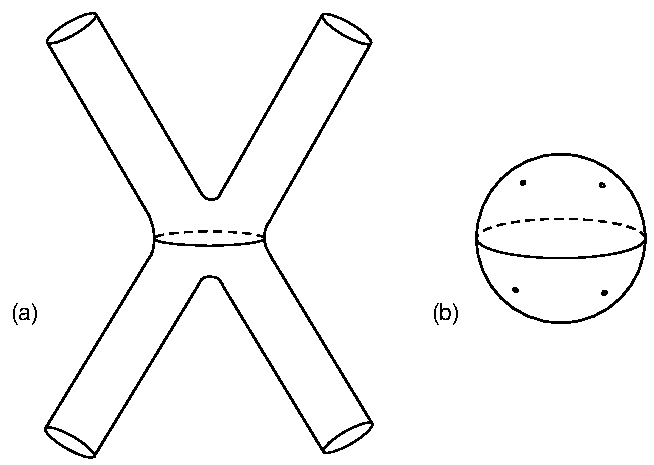
\includegraphics[width=0.8\linewidth]{figures/fig_3_8.pdf}
\caption{(a) 源が $X^0=\pm\infty$ に近づく、四本の閉弦の散乱。(b) 四本の閉弦の散乱を表す共形的に等価な描像。小さな穴をもつ球面となる。}
\label{fig:3.8}
\end{figure}

第2章から知っているように、円筒は座標 $z$ によって共形的に等価に記述できる。
\begin{equation}
z=\exp(-iw),\qquad \exp(-2\pi t)\leq|z|\leq1.
\tag{3.5.2}\label{eq:3.5.2}
\end{equation}
この描像では、長い円筒が単位円板に写され、外部の弦状態は中心にある小さな円になる。内部計量の幾何では、図\hyperref[fig:3.8]{3.8}(a)の過程は、今や図\hyperref[fig:3.8]{3.8}(b)のように見える。$t\to\infty$ の極限では、小さな円は点へ縮み、世界面は、外部状態ごとに一点の挿入をもつ球面に帰着する。

同じ考えは、外部の開弦状態にも成り立つ。図\hyperref[fig:3.9]{3.9}(a)の過程における長い帯は、領域
\begin{equation}
-2\pi t\leq\operatorname{Im}w\leq0,\qquad
0\leq\operatorname{Re}w\leq\pi
\tag{3.5.3}\label{eq:3.5.3}
\end{equation}
として記述できる。$\operatorname{Im}w=-2\pi t$ が源であり、$\operatorname{Re}w=0,\pi$ は弦の端点の境界である。$z=-\exp(-iw)$ の下で、これは単位円板と上半平面の共通部分から、原点の小さな半円を切り取ったものに写る。
\begin{equation}
\exp(-2\pi t)\leq|z|\leq1,\qquad \operatorname{Im}z\geq0.
\tag{3.5.4}\label{eq:3.5.4}
\end{equation}
散乱過程は、今や図\hyperref[fig:3.9]{3.9}(b)のように見える。$t\to\infty$ の極限では、源は（弦の端点の）境界上の点へ縮む。

\begin{figure}[htbp]
\centering
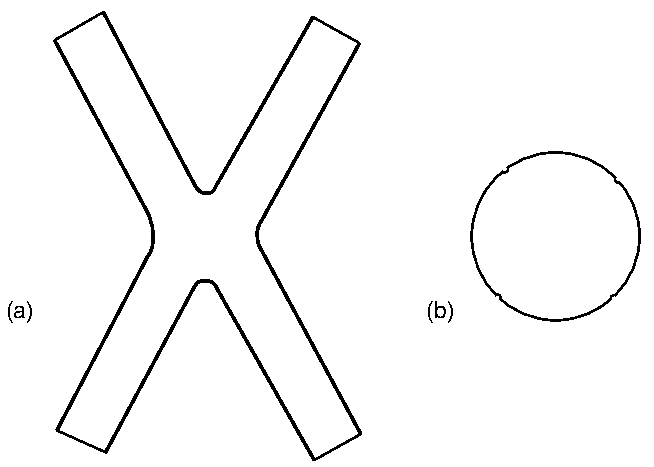
\includegraphics[width=0.8\linewidth]{figures/fig_3_9.pdf}
\caption{(a) 源が $X^0=\pm\infty$ に近づく、四本の開弦の散乱。(b) 共形的に等価な描像。小さなくぼみをもつ円板となる。}
\label{fig:3.9}
\end{figure}

これは、すでに見た状態・演算子対応である。各弦の源は、世界面上の局所的な擾乱となる。$D$ 元運動量 $k^\mu$ と内部状態 $j$ をもつ、与えられた入射または出射の弦には、この極限操作によって決まる局所的な頂点演算子 $\mathcal V_j(k)$ が対応する。入射状態と出射状態は $k^0$ の符号によって区別され、入射状態では $k^\mu=(E,\mathbf k)$、出射状態では $k^\mu=-(E,\mathbf k)$ である。図\hyperref[fig:3.8]{3.8}と\hyperref[fig:3.9]{3.9}は最低次の振幅だけを描いているが、この構成が一般的であることは明らかである。無限遠に伸びる管をもたず、その代わりに、各外部閉弦に対して内部に一点の挿入を、各外部開弦に対して境界上に一点の挿入をもつ、コンパクトな世界面に注意を限ることができる。すると、$n$ 粒子の $S$ 行列要素は
\begin{equation}
\begin{aligned}
S_{j_1\cdots j_n}(k_1,\ldots,k_n)
={}&\sum_{\substack{\text{コンパクトな}\\\text{位相型}}}
\int\frac{[dX\,dg]}{V_{\mathrm{diff}\times\mathrm{Weyl}}}
\exp(-S_X-\lambda\chi)\\
&\quad\times\prod_{i=1}^n
\int d^2\sigma_i\,g(\sigma_i)^{1/2}
\mathcal V_{j_i}(k_i,\sigma_i)
\end{aligned}
\tag{3.5.5}\label{eq:3.5.5}
\end{equation}
によって与えられる。頂点演算子の挿入を微分同相不変にするため、世界面上でそれらを積分した。第1巻の残りでは、この推測が正しく、これが実際に意味のある弦の $S$ 行列を定義することを見るであろう。

四種類の弦理論のうちどれを考えるかに応じて、位相型についての和には、向き付けのない世界面や、境界をもつ世界面、あるいはその両方が含まれる。一般に、位相型についての和は連結な世界面だけに制限されない。全過程には、互いに遠く離れた二組以上の粒子群が独立に散乱する過程が含まれうる。和を連結な曲面に制限して得られる、連結な $S$ 行列に注目すると便利である。

したがって、連結な $S$ 行列を得るには、世界面のコンパクトで連結なすべての位相型について和をとらねばならない。二次元では、そのような位相型の分類はよく知られている。境界をもたない、コンパクトで連結かつ向き付けられた任意の二次元曲面は、$g$ 個の取っ手を付けた球面と位相的に同値である。$g$ は曲面の種数と呼ばれる。図\hyperref[fig:3.10]{3.10}に $g=0,1,2$ を示す。閉曲面に穴を開ければ、境界を加えられる。コンパクトで連結かつ向き付けられた任意の二次元曲面は、$g$ 個の取っ手と $b$ 個の穴をもつ球面に位相的に同値である。たとえば、$(g,b)=(0,1)$ は円板、$(0,2)$ は円環、$(0,3)$ はズボン型曲面である。

\begin{figure}[htbp]
\centering
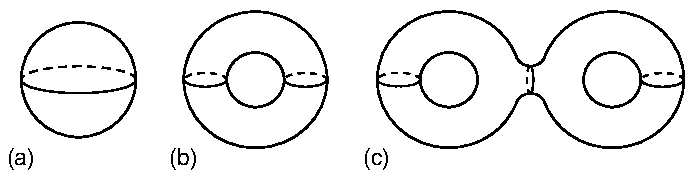
\includegraphics[width=0.8\linewidth]{figures/fig_3_10.pdf}
\caption{種数が (a) 0、(b) 1、(c) 2 の、コンパクトで連結かつ向き付けられた閉曲面。}
\label{fig:3.10}
\end{figure}

向き付けのない曲面を記述するには、クロスキャップを導入すると便利である。曲面に穴を開け、直径の両端にある点を同一視するのである。より詳しくは、複素座標 $z$ をとり、半径が1よりわずかに小さい円板を切り取り、$z'=-1/\bar z$ を満たす点の対を等価と定義することによって、向かい合う点を貼り合わせる。貼り合わせが反正則なので、得られる曲面は向き付けをもたない。また、境界の場合と違って、クロスキャップは縁などの局所的な特徴を導入しない。切り取ることで導入された縁は、単に座標パッチの境界である。向き付けの有無を問わず、コンパクトで連結な任意の閉曲面は、球面に $g$ 個の取っ手と $c$ 個のクロスキャップを加えることで得られる。コンパクトで連結な任意の曲面は、球面に $g$ 個の取っ手、$b$ 個の境界、$c$ 個のクロスキャップを加えることで得られる。実際には、この記述にはいくらか冗長性がある。境界がある場合もない場合も、$g$ と $c$ の両方が同時にゼロでない値をとらないように和を制限すれば、すべての位相型をちょうど一度ずつ得る。たとえば、$(g,b,c)=(0,0,1)$ は射影平面、$(g,b,c)=(0,1,1)$ は Möbius の帯、$(g,b,c)=(0,0,2)$ は Klein の壺である。また、クロスキャップを付けたトーラスは、二つのクロスキャップを一つの取っ手に置き換えることにより、$(g,b,c)=(0,0,3)$ としても $(g,b,c)=(1,0,1)$ としても得られる。Euler 数は
\begin{equation}
\chi=2-2g-b-c
\tag{3.5.6}\label{eq:3.5.6}
\end{equation}
で与えられる。

異なる位相型の数は、場の理論の一定の次数における異なる Feynman 図の数に比べて非常に少ない。たとえば、向き付けられた閉弦の理論では、摂動論の各次数に位相型がちょうど一つ存在する。場の理論では、図の数は次数に対して階乗的に増える。一つの弦の図には、場の理論のすべての図が含まれている。取っ手がその周長に比べて長くなるさまざまな極限では、取っ手を線で近似でき、その極限の弦の図は、対応する Feynman 図で近似される。

\subsectionlink{頂点演算子}
\label{sec:3.6}

状態と演算子の写像を用いると、閉弦のタキオンの頂点演算子は
\begin{equation}
\begin{aligned}
V_0&=2g_{\mathrm c}\int d^2\sigma\,g^{1/2}e^{ik\cdot X}\\
&\longrightarrow g_{\mathrm c}\int d^2z\,:e^{ik\cdot X}:.
\end{aligned}
\tag{3.6.1}\label{eq:3.6.1}
\end{equation}
ここでは、写像に因子 $g_{\mathrm c}$ を含めた。これは過程に弦をもう一本加えることから生じる閉弦の結合定数であり、頂点演算子の規格化を結合の定義として用いる。第2行では平坦な世界面へ移った。頂点演算子は $(\mathrm{diff}\times\mathrm{Weyl})$ 不変でなければならず、とくに平坦な世界面上で共形不変でなければならない。$d^2z$ の変換を相殺するため、演算子は共形ウェイト $(1,1)$ のテンソルでなければならない。直接的な OPE の計算により、$e^{ik\cdot X}$ は共形ウェイト $h=\widetilde h=\alpha'k^2/4$ のテンソルなので、条件は
\begin{equation}
m^2=-k^2=-\frac4{\alpha'}.
\tag{3.6.2}\label{eq:3.6.2}
\end{equation}
これは光円錐量子化で得られた質量と正確に一致する。

同様に、閉弦の最初の励起レベルにあるテンソル状態は、平坦な世界面上の頂点演算子
\begin{equation}
\frac{2g_{\mathrm c}}{\alpha'}\int d^2z\,
:\partial X^\mu\bar\partial X^\nu e^{ik\cdot X}:
\tag{3.6.3}\label{eq:3.6.3}
\end{equation}
を持つ。タキオンの頂点演算子に対する相対的な規格化は、状態と演算子の写像から従う。第6章では、S 行列のユニタリー性からも同じ相対規格化が得られることを見る。共形ウェイトは
\begin{equation}
h=\widetilde h=1+\frac{\alpha'k^2}{4}
\tag{3.6.4}\label{eq:3.6.4}
\end{equation}
なので、これらは質量ゼロであり、再び光円錐量子化と一致する。これがテンソルとなるにはさらに条件があり、以下で求める。

\subsubsectionlink*{Polyakov の方法における頂点演算子}

状態と演算子の写像は、任意の状態の平坦な世界面上の頂点演算子を書くための系統的な手段を与える。世界面はつねに局所的に平坦にできるので、原理的にはこれだけで十分である。しかし見通しを得るためには、Polyakov 形式における曲がった世界面上の頂点演算子を調べると有用である。この節の残りではそれを行う。用いる方法はやや煩雑で、状態と演算子の写像ほど系統的ではないが、結果の一部は役立つ。読者はすべての詳細を計算する必要はない。

Polyakov 経路積分 \hyperref[eq:3.5.5]{(3.5.5)} に含める演算子は、理論の局所的な $\mathrm{diff}\times\mathrm{Weyl}$ 対称性を保たなければならない。式 \hyperref[eq:3.6.1]{(3.6.1)} の第1行では、曲がった世界面上で演算子をどう定義するかを具体的には述べなかった。先の Weyl 異常の議論と同様に、diff 不変性を自動的に保つ方法を用い、Weyl 変換は直接調べるのが便利である。文献では多くの目的に次元正則化が使われる。しかし、ここではそれを広く使う必要はないので導入せず、以前に導入した正規順序を一般化する。繰り込まれた演算子 $[\mathcal F]_{\mathrm r}$ を
\begin{equation}
[\mathcal F]_{\mathrm r}=
\exp\left(\frac12\int d^2\sigma\,d^2\sigma'\,
\Delta(\sigma,\sigma')
\frac{\delta}{\delta X^\mu(\sigma)}
\frac{\delta}{\delta X_\mu(\sigma')}\right)\mathcal F
\tag{3.6.5}\label{eq:3.6.5}
\end{equation}
によって定義する。ここで
\begin{equation}
\Delta(\sigma,\sigma')=\frac{\alpha'}2\ln d^2(\sigma,\sigma')
\tag{3.6.6}\label{eq:3.6.6}
\end{equation}
であり、$d(\sigma,\sigma')$ は点 $\sigma$ と $\sigma'$ の間の測地距離である。正規順序と同様に、式 \hyperref[eq:3.6.5]{(3.6.5)} は、$\Delta(\sigma,\sigma')$ を用いて $\mathcal F$ 内の対を縮約するすべての方法について和を取ることを指示している。平坦な世界面では $d^2(\sigma,\sigma')=|z-z'|^2$ なので、詳しく調べた共形正規順序へ帰着する。曲がった世界面では、$\mathcal F$ 内の場の自己縮約の特異部分を相殺する。diff 不変性は明らかだが、縮約は計量に依存するため、Weyl 依存性
\begin{equation}
\begin{aligned}
\delta_{\mathrm W}[\mathcal F]_{\mathrm r}
&=[\delta_{\mathrm W}\mathcal F]_{\mathrm r}\\
&\quad+\frac12\int d^2\sigma\,d^2\sigma'\,
\delta_{\mathrm W}\Delta(\sigma,\sigma')
\frac{\delta}{\delta X^\mu(\sigma)}
\frac{\delta}{\delta X_\mu(\sigma')}[\mathcal F]_{\mathrm r}
\end{aligned}
\tag{3.6.7}\label{eq:3.6.7}
\end{equation}
が導入される。第1項は演算子に明示的に含まれる Weyl 依存性である。

運動量 $k^\mu$ の状態の頂点演算子は、並進の下でその状態と同じように変換しなければならないので、$e^{ik\cdot X}$ に $X^\mu$ の微分を掛けた形になる。微分の数が異なる演算子は Weyl 変換で混ざらないので、まず微分がゼロ個の場合、すなわち演算子 \hyperref[eq:3.6.1]{(3.6.1)} から考えられる。Weyl 変分は、明示的な因子 $g^{1/2}$ と、式 \hyperref[eq:3.6.7]{(3.6.7)} に示した繰り込みの両方から生じる：
\begin{equation}
\delta_{\mathrm W}V_0
=2g_{\mathrm c}\int d^2\sigma\,g^{1/2}
\left(2\delta\omega(\sigma)
-\frac{k^2}{2}\delta_{\mathrm W}\Delta(\sigma,\sigma)\right)
[e^{ik\cdot X(\sigma)}]_{\mathrm r}.
\tag{3.6.8}\label{eq:3.6.8}
\end{equation}
短距離では
\begin{equation}
d^2(\sigma,\sigma')\approx
(\sigma-\sigma')^2\exp(2\omega(\sigma))
\tag{3.6.9}\label{eq:3.6.9}
\end{equation}
であり、したがって
\begin{equation}
\Delta(\sigma,\sigma')\approx
\alpha'\omega(\sigma)+\frac{\alpha'}2\ln(\sigma-\sigma')^2.
\tag{3.6.10}\label{eq:3.6.10}
\end{equation}
Weyl 変分は $\sigma'\to\sigma$ の極限で非特異であり、
\begin{equation}
\delta_{\mathrm W}\Delta(\sigma,\sigma)=\alpha'\delta\omega(\sigma).
\tag{3.6.11}\label{eq:3.6.11}
\end{equation}
すると Weyl 変分 \hyperref[eq:3.6.8]{(3.6.8)} がゼロとなる条件は、上ですでに導いたように $k^2=4/\alpha'$ となる。

\subsubsectionlink*{オフシェル振幅？}

$k^\mu$ を質量殻から外してオフシェル振幅を定義しようとする素朴な試みは、世界面の局所対称性と整合しないことに注意しよう。位置空間では、これは経路積分に
\begin{equation}
\delta^D(X(\sigma)-x_0)=
\int\frac{d^Dk}{(2\pi)^D}
\exp[ik\cdot(X(\sigma)-x_0)]
\tag{3.6.12}\label{eq:3.6.12}
\end{equation}
を挿入して与えられる、弦の世界面の局所的な探査が、あらゆる運動量を含むため整合しないことを意味する。

いくつかの観点から、これは驚くべきことではない。第1に、弦状態に点状の源（頂点演算子）を使えるとした上の議論には、実質的にオンシェルの問題へ制限する極限操作が必要であった。第2に、弦理論は重力を含み、一般相対論には単純なオフシェル振幅は存在しない。探査を行う位置を指定しなければならないが、座標は物理的なものではなく、座標不変なオフシェル量ははるかに複雑だからである。第3に、弦理論では、局所的な観測量を測定するために追加の場を導入する自由はない（強く相互作用する系を探るために電弱過程を使うのと同様のことはできない）。弦そのものか、これから論じる、理論に内在するほかの物体（D ブレーンやソリトン）を用いなければならない。

ゲージを固定し（この目的には光円錐ゲージが最も簡単である）、弦状の源を用いれば、少なくとも摂動論ではオフシェル振幅を定義できる。その場合、S 行列の公式 \hyperref[eq:3.5.5]{(3.5.5)} は、場の量子論の還元公式により近い形で導ける。有限時間の遷移振幅を定義した後、無限時間の極限を取ることが可能だからである。なお、現在の議論と場の理論の関係を理解しようとしている読者は、経路積分の式 \hyperref[eq:3.5.5]{(3.5.5)} が Green 関数に対応するのではなく、実際には S 行列要素の性質を持つことに注意してほしい。場の理論で対応するのは、外線の伝播関数を切断し、外部運動量を質量殻上に制限した Green 関数である。

局所的探査 \hyperref[eq:3.6.12]{(3.6.12)} の議論は、弦同士の接触相互作用の問題点も示している。そのような相互作用の最も簡単な形は
\begin{equation}
\int_M d^2\sigma\,g(\sigma)^{1/2}
\int_M d^2\sigma'\,g(\sigma')^{1/2}
\delta^D(X(\sigma)-X(\sigma'))
\tag{3.6.13}\label{eq:3.6.13}
\end{equation}
であり、世界面が自己交差するたびにゼロでない値を取る。しかし、デルタ関数は式 \hyperref[eq:3.6.12]{(3.6.12)} と同じくあらゆる運動量を含むので、これは Weyl 不変ではない。弦理論の構造はかなり強く制約されている。弦と弦が結合できるのは、この章の初めに述べた方法によってだけである。

\subsubsectionlink*{質量ゼロの閉弦の頂点演算子}

頂点演算子の Polyakov による取り扱いをもう一つ上のレベルへ進めることは、少し煩雑ではあるが興味深い。微分をちょうど一つ含む世界面スカラーを作ることはできないので、次の場合は微分が二つである。diff 不変な可能性は
\begin{equation}
\begin{aligned}
V_1=\frac{g_{\mathrm c}}{\alpha'}\int d^2\sigma\,g^{1/2}
\Bigl\{&(g^{ab}s_{\mu\nu}+i\epsilon^{ab}a_{\mu\nu})
[\partial_aX^\mu\partial_bX^\nu e^{ik\cdot X}]_{\mathrm r}\\
&+\alpha'\phi R[e^{ik\cdot X}]_{\mathrm r}\Bigr\},
\end{aligned}
\tag{3.6.14}\label{eq:3.6.14}
\end{equation}
である。ここで $s_{\mu\nu}$、$a_{\mu\nu}$、$\phi$ はそれぞれ対称行列、反対称行列、定数である。反対称テンソル $\epsilon^{ab}$ は $g^{1/2}\epsilon^{12}=1$、あるいは $g^{1/2}\epsilon^{z\bar z}=-i$ と規格化する。頂点演算子で反対称テンソルに付く $i$ は、Euclid 化から生じると理解できる。この項は必ず奇数個（一つ）の時間微分を含むからである。この結果は、Euclid 作用と頂点演算子に一般的に当てはまる。

Weyl 不変性の解析を拡張するには、測地距離の Weyl 依存性 \hyperref[eq:3.6.11]{(3.6.11)} を高次まで求める必要がある。結果は
\begin{align}
\left.\partial_a\delta_{\mathrm W}\Delta(\sigma,\sigma')
\right|_{\sigma'=\sigma}
&=\frac12\alpha'\partial_a\delta\omega(\sigma),
\tag{3.6.15a}\label{eq:3.6.15a}\\
\left.\partial_a\partial'_b\delta_{\mathrm W}\Delta(\sigma,\sigma')
\right|_{\sigma'=\sigma}
&=\frac{1+\gamma}{2}\alpha'\nabla_a\partial_b\delta\omega(\sigma),
\tag{3.6.15b}\label{eq:3.6.15b}\\
\left.\nabla_a\partial_b\delta_{\mathrm W}\Delta(\sigma,\sigma')
\right|_{\sigma'=\sigma}
&=-\frac{\gamma}{2}\alpha'\nabla_a\partial_b\delta\omega(\sigma).
\tag{3.6.15c}\label{eq:3.6.15c}
\end{align}
ここで $\gamma=-\frac23$ だが、後で参照するためにパラメーターとして残しておいた。第3式は、第2式と第1式の勾配から得られる。曲率の変分には式 \hyperref[eq:3.3.5]{(3.3.5)} を、繰り込みの変分には式 \hyperref[eq:3.6.7]{(3.6.7)} と \hyperref[eq:3.6.15a]{(3.6.15)} を用いると、
\begin{equation}
\begin{aligned}
\delta_{\mathrm W}V_1
=\frac{g_{\mathrm c}}2\int d^2\sigma\,g^{1/2}\delta\omega\,
\Bigl\{&(g^{ab}S_{\mu\nu}+i\epsilon^{ab}A_{\mu\nu})
[\partial_aX^\mu\partial_bX^\nu e^{ik\cdot X}]_{\mathrm r}\\
&+\alpha'FR[e^{ik\cdot X}]_{\mathrm r}\Bigr\},
\end{aligned}
\tag{3.6.16}\label{eq:3.6.16}
\end{equation}
ここで
\begin{align}
S_{\mu\nu}
&=-k^2s_{\mu\nu}+k_\nu k^\omega s_{\mu\omega}
+k_\mu k^\omega s_{\nu\omega}
-(1+\gamma)k_\mu k_\nu s^\omega{}_\omega
+4k_\mu k_\nu\phi,
\tag{3.6.17a}\label{eq:3.6.17a}\\
A_{\mu\nu}
&=-k^2a_{\mu\nu}+k_\nu k^\omega a_{\mu\omega}
-k_\mu k^\omega a_{\nu\omega},
\tag{3.6.17b}\label{eq:3.6.17b}\\
F&=(\gamma-1)k^2\phi+\frac12\gamma k^\mu k^\nu s_{\mu\nu}
-\frac14\gamma(1+\gamma)k^2s^\nu{}_\nu.
\tag{3.6.17c}\label{eq:3.6.17c}
\end{align}

Weyl 変分 \hyperref[eq:3.6.16]{(3.6.16)} の導出では部分積分を行い、さらに関係
\begin{equation}
[\nabla^2X^\mu e^{ik\cdot X}]_{\mathrm r}
=i\frac{\alpha'\gamma}{4}k^\mu R[e^{ik\cdot X}]_{\mathrm r}
\tag{3.6.18}\label{eq:3.6.18}
\end{equation}
を用いた。素朴な運動方程式によれば左辺はゼロになるはずだが、ここでは運動方程式に同じ点の別の演算子が掛かっている。この場合に成り立つ一般原理は、この演算子は必ずしもゼロではないが独立ではなく、理論のほかの局所演算子によって展開できる、というものである。一般に、これらの演算子の係数は繰り込み方式に依存する。結果 \hyperref[eq:3.6.18]{(3.6.18)} は、両辺の Weyl 変分を取って求められる。

$S_{\mu\nu}$、$A_{\mu\nu}$、$F$ は独立な演算子に掛かっているので、Weyl 不変性の条件は
\begin{equation}
S_{\mu\nu}=A_{\mu\nu}=F=0.
\tag{3.6.19}\label{eq:3.6.19}
\end{equation}
演算子の数を正しく数えるには、形 \hyperref[eq:3.6.14]{(3.6.14)} のすべての $V_1$ が独立ではないことに注意しなければならない。実際、
\begin{align}
s_{\mu\nu}&\longrightarrow s_{\mu\nu}+\xi_\mu k_\nu+k_\mu\xi_\nu,
\tag{3.6.20a}\label{eq:3.6.20a}\\
a_{\mu\nu}&\longrightarrow a_{\mu\nu}+\zeta_\mu k_\nu-k_\mu\zeta_\nu,
\tag{3.6.20b}\label{eq:3.6.20b}\\
\phi&\longrightarrow\phi+\frac{\gamma}{2}k\cdot\xi
\tag{3.6.20c}\label{eq:3.6.20c}
\end{align}
の下で、$V_1$ の変化は、運動方程式 \hyperref[eq:3.6.18]{(3.6.18)} を用いると積分してゼロになる。ここで $n\cdot k=1$、$n^2=0$ を満たすベクトル $n^\mu$ を選ぶ。独立な演算子の完全な組は、
\begin{equation}
n^\mu s_{\mu\nu}=n^\mu a_{\mu\nu}=0
\tag{3.6.21}\label{eq:3.6.21}
\end{equation}
に制限して得られる。これは $2D$ 個のパラメーター $\xi_\mu$ と $\zeta_\mu$ に対する $2D$ 本の方程式である。一つの方程式と一つのパラメーターは自明だが、それ以外について式 \hyperref[eq:3.6.21]{(3.6.21)} は非退化であり、独立な頂点演算子の組を定義することを示せる。

条件 \hyperref[eq:3.6.21]{(3.6.21)} を用いて、まず $S_{\mu\nu}n^\mu n^\nu=0$、次に $S_{\mu\nu}n^\mu=A_{\mu\nu}n^\mu=0$、最後に完全な条件 $S_{\mu\nu}=A_{\mu\nu}=F=0$ を解くと、
\begin{align}
k^2&=0,
\tag{3.6.22a}\label{eq:3.6.22a}\\
k^\nu s_{\mu\nu}&=k^\mu a_{\mu\nu}=0,
\tag{3.6.22b}\label{eq:3.6.22b}\\
\phi&=\frac{1+\gamma}{4}s^\mu{}_\mu
\tag{3.6.22c}\label{eq:3.6.22c}
\end{align}
が得られる。再び質量殻条件 \hyperref[eq:3.6.22a]{(3.6.22a)} が得られ、今度は閉弦の最初の励起状態に対応している。また、質量ゼロのテンソル場の物理的な偏極に必要な、偏極が運動量に対して横向きであるという条件 \hyperref[eq:3.6.22b]{(3.6.22b)} もある。
\begin{equation}
k^\mu=(1,1,0,0,\ldots,0),\qquad
n^\mu=\frac12(-1,1,0,0,\ldots,0)
\tag{3.6.23}\label{eq:3.6.23}
\end{equation}
となる系では、条件 \hyperref[eq:3.6.21]{(3.6.21)} と \hyperref[eq:3.6.22b]{(3.6.22b)} から0成分と1成分がすべてゼロとなり、式 \hyperref[eq:3.6.22c]{(3.6.22c)} が $\phi$ を固定する。残る独立な演算子は正確に $(D-2)^2$ 個であり、光円錐ゲージで得られた質量ゼロの閉弦状態の数と同じである。

条件 $n^\mu s_{\mu\nu}=n^\mu a_{\mu\nu}=0$ は、ノルムがゼロの光的な偏極を除くために必要である。しかし、ベクトル $n^\mu$ の導入は顕在的な Lorentz 不変性を損なう。理論が Lorentz 不変であるのは、\hyperref[eq:3.6.20a]{(3.6.20)} により $n^\mu$ の異なる選択が等価であるからにほかならない。したがって、同値関係 \hyperref[eq:3.6.20a]{(3.6.20)} は、正の Hilbert 空間ノルムを持つ Lorentz 不変な理論を得るために不可欠である。これらの関係は、時空の局所対称性が存在するしるしである。とくに $\xi_\mu$ は時空の無限小座標変換であり、$\zeta_\mu$ は反対称テンソル場の時空の局所対称性である。第1.4節では、質量ゼロのスピン1場とスピン2場があるために時空の局所対称性が存在しなければならないと論じたが、今や相互作用する理論でその存在が見えた。

触れておくべき技術的な点がある。異なる繰り込み方式では、繰り込まれた演算子に異なる名前を付ける。最もよく使われる方式は次元正則化であり、この方式での演算子と上の方式での演算子の関係は
\begin{align}
[e^{ik\cdot X}]_{\mathrm{DR}}
&=[e^{ik\cdot X}]_{\mathrm r},
\tag{3.6.24a}\label{eq:3.6.24a}\\
[\partial_aX^\mu e^{ik\cdot X}]_{\mathrm{DR}}
&=[\partial_aX^\mu e^{ik\cdot X}]_{\mathrm r},
\tag{3.6.24b}\label{eq:3.6.24b}\\
[\partial_aX^\mu\partial_bX^\nu e^{ik\cdot X}]_{\mathrm{DR}}
&=[\partial_aX^\mu\partial_bX^\nu e^{ik\cdot X}]_{\mathrm r}
-\frac{\alpha'}{12}g_{ab}\eta^{\mu\nu}R[e^{ik\cdot X}]_{\mathrm r},
\tag{3.6.24c}\label{eq:3.6.24c}\\
[\nabla_a\partial_bX^\mu e^{ik\cdot X}]_{\mathrm{DR}}
&=[\nabla_a\partial_bX^\mu e^{ik\cdot X}]_{\mathrm r}
+i\frac{\alpha'}{12}g_{ab}k^\mu R[e^{ik\cdot X}]_{\mathrm r}.
\tag{3.6.24d}\label{eq:3.6.24d}
\end{align}
式 \hyperref[eq:3.6.18]{(3.6.18)} と比較すると、次元正則化では $\gamma=0$ であり、正則化された演算子の内部で運動方程式が成り立つと分かる。これは便利で、多くの式が簡単になる。とくに、時空のゲージ変換 \hyperref[eq:3.6.20a]{(3.6.20)} では $\phi$ は不変である。

\subsubsectionlink*{開弦の頂点演算子}

開弦への拡張は直接的である。詳細は演習3.9として読者に任せ、いくつかの結果だけを示す。タキオンの頂点演算子は
\begin{equation}
g_{\mathrm o}\int_{\partial M}ds\,[e^{ik\cdot X}]_{\mathrm r}
\tag{3.6.25}\label{eq:3.6.25}
\end{equation}
であり、$k^2=1/\alpha'$ で Weyl 不変となる。光子の頂点演算子は
\begin{equation}
-i\frac{g_{\mathrm o}}{(2\alpha')^{1/2}}e_\mu
\int_{\partial M}ds\,[\dot X^\mu e^{ik\cdot X}]_{\mathrm r}.
\tag{3.6.26}\label{eq:3.6.26}
\end{equation}
タキオンに対する相対規格化は状態と演算子の写像またはユニタリー性から得られ、$i$ は閉弦の頂点演算子 \hyperref[eq:3.6.14]{(3.6.14)} について論じたとおりであり、符号は規約の問題である。この演算子は $k^2=0$、$k\cdot e=0$ ならば Weyl 不変である。同値関係 $e_\mu\cong e_\mu+\lambda k_\mu$ があり、これは時空のゲージ変換である。これにより $D-2$ 個の横方向の偏極が残る。

\subsectionlink{曲がった時空の中の弦}
\label{sec:3.7}

これで、新しい重要な問題、すなわち曲がった時空の中を運動する弦を考える準備ができた。まず、点粒子の作用には曲がった時空への自然な拡張があることを思い出そう。平坦な計量 $\eta_{\mu\nu}$ を一般の計量 $G_{\mu\nu}(x)$ に置き換えると、作用
\begin{equation}
S_{\mathrm{pp}}=\frac12\int d\tau
\left(\eta^{-1}G_{\mu\nu}(X)\dot X^\mu\dot X^\nu-\eta m^2\right)
\tag{3.7.1}\label{eq:3.7.1}
\end{equation}
を得る。$\eta$ を消去すると、これは粒子の世界線に沿った不変な固有時間となる。その変分が測地線方程式を与え、重力場の中の粒子の運動を表すことはよく知られている。

Polyakov 作用で同じ置き換えを行うと、
\begin{equation}
S_\sigma=\frac1{4\pi\alpha'}\int_M d^2\sigma\,g^{1/2}g^{ab}
G_{\mu\nu}(X)\partial_aX^\mu\partial_bX^\nu.
\tag{3.7.2}\label{eq:3.7.2}
\end{equation}
これは自然な推測だが、読者は次のように反論するかもしれない。重力子自身が弦の一状態であることを学んだ。曲がった時空は、大まかにいえば重力子のコヒーレントな背景であり、したがって弦理論では弦のコヒーレント状態である。曲がった計量を作用 \hyperref[eq:3.7.2]{(3.7.2)} に入れるだけでは、弦の性質を十分に反映していないように見える。これが正当化される理由を見るため、平坦に近い時空
\begin{equation}
G_{\mu\nu}(X)=\eta_{\mu\nu}+\chi_{\mu\nu}(X)
\tag{3.7.3}\label{eq:3.7.3}
\end{equation}
を、$\chi_{\mu\nu}$ が小さいとして考える。世界面の経路積分の被積分関数は
\begin{equation}
\begin{aligned}
\exp(-S_\sigma)=\exp(-S_{\mathrm P})
\Bigl[1-\frac1{4\pi\alpha'}\int_M d^2\sigma\,
g^{1/2}g^{ab}\chi_{\mu\nu}(X)
\partial_aX^\mu\partial_bX^\nu+\cdots\Bigr].
\end{aligned}
\tag{3.7.4}\label{eq:3.7.4}
\end{equation}
$\chi$ の1次の項は、まさに弦の重力子状態の頂点演算子、式 \hyperref[eq:3.6.14]{(3.6.14)} で
\begin{equation}
\chi_{\mu\nu}(X)=-4\pi g_{\mathrm c}e^{ik\cdot X}s_{\mu\nu}
\tag{3.7.5}\label{eq:3.7.5}
\end{equation}
としたものである。したがって、曲がった計量を挿入することは、確かに既知の結果と結びついているようである。作用 \hyperref[eq:3.7.2]{(3.7.2)} は、重力子の頂点演算子を指数化することによって、重力子のコヒーレント状態を記述していると考えられる。

これは自然な一般化を示唆する。ほかの質量ゼロの弦状態の背景も含めればよい。頂点演算子の形、式 \hyperref[eq:3.6.14]{(3.6.14)}、から
\begin{equation}
\begin{aligned}
S_\sigma=\frac1{4\pi\alpha'}\int_M d^2\sigma\,g^{1/2}
\Bigl[&(g^{ab}G_{\mu\nu}(X)+i\epsilon^{ab}B_{\mu\nu}(X))
\partial_aX^\mu\partial_bX^\nu\\
&+\alpha'R\Phi(X)\Bigr].
\end{aligned}
\tag{3.7.6}\label{eq:3.7.6}
\end{equation}
場 $B_{\mu\nu}(X)$ は反対称テンソルであり、ディラトンには、運動方程式 \hyperref[eq:3.6.22c]{(3.6.22c)} が示すように、$\Phi$ と $G_{\mu\nu}$ の対角部分の両方が関わる。

確認のため、時空のゲージ不変性が保たれることを見よう。場の再定義 $X'^\mu(X)$ に対応する経路積分の変数変換の下で、$G_{\mu\nu}$ と $B_{\mu\nu}$ がテンソル、$\Phi$ がスカラーとして変換すれば、作用 \hyperref[eq:3.7.6]{(3.7.6)} は不変である。時空の観点では、これは座標変換である。作用はまた、
\begin{equation}
\delta B_{\mu\nu}(X)=\partial_\mu\zeta_\nu(X)-\partial_\nu\zeta_\mu(X)
\tag{3.7.7}\label{eq:3.7.7}
\end{equation}
の下でも不変であり、この変換は Lagrangian 密度に全微分を加える。これは、電磁ゲージ変換を、二つの反対称な添字を持つポテンシャルへ一般化したものである。三つの添字を持つ場の強さ
\begin{equation}
H_{\omega\mu\nu}=
\partial_\omega B_{\mu\nu}+\partial_\mu B_{\nu\omega}
+\partial_\nu B_{\omega\mu}
\tag{3.7.8}\label{eq:3.7.8}
\end{equation}
は不変である。反対称な $n$ 階テンソルポテンシャルへの同様の一般化もあり、超弦で重要な役割を果たすので第2巻で展開する。

したがって理論は、計量とほかの場から作られるゲージ不変な量だけに依存する。場 $X^\mu$ は多様体上の座標であると考えられる。この多様体を標的空間と呼ぶのは、$X^\mu$ が埋め込み
\begin{equation}
\text{世界面}\ \longrightarrow\ \text{標的空間}
\tag{3.7.9}\label{eq:3.7.9}
\end{equation}
を定義するからである。弦理論では、標的空間は時空そのものである。\hyperref[eq:3.7.2]{(3.7.2)} のように、運動項が場に依存し、そのため場の空間が実質的に曲がった多様体となる場の理論は、歴史的な理由から非線形シグマ模型として知られている。非線形シグマ模型には、素粒子物理や場の量子論で多くの応用がある。たとえば、中性および荷電パイ中間子の場は、よい近似で群多様体 $SU(2)$ 上の座標とみなせる。

非線形シグマ模型の作用は、もはや $X^\mu$ の2次式ではないため、経路積分は今や相互作用する2次元の場の量子論である。任意に選んだ点 $x_0^\mu$ に対する古典解 $X^\mu(\sigma)=x_0^\mu$ の周りで経路積分を展開する。$X^\mu(\sigma)=x_0^\mu+Y^\mu(\sigma)$ とすると、
\begin{equation}
\begin{aligned}
G_{\mu\nu}(X)\partial_aX^\mu\partial_bX^\nu
=\Bigl[&G_{\mu\nu}(x_0)+G_{\mu\nu,\omega}(x_0)Y^\omega\\
&+\frac12G_{\mu\nu,\omega\rho}(x_0)Y^\omega Y^\rho+\cdots\Bigr]
\partial_aY^\mu\partial_bY^\nu.
\end{aligned}
\tag{3.7.10}\label{eq:3.7.10}
\end{equation}
この展開の第1項は、場 $Y^\mu$ の2次の運動項である。次の項は3次の相互作用であり、以下同様である。展開の結合定数 $G_{\mu\nu,\omega}(x_0)$ などは、$x_0$ における計量の微分を含む。特徴的な曲率半径が $R_{\mathrm c}$ の標的空間では、計量の微分は $R_{\mathrm c}^{-1}$ 程度である。したがって、理論の有効な無次元結合は $\alpha'^{1/2}R_{\mathrm c}^{-1}$ となる。曲率半径 $R_{\mathrm c}$ が弦の特徴的な長さスケールよりはるかに大きければ、この結合は小さく、2次元場の理論の摂動論が有用な道具になる。同じ領域では、もう一つの道具も使えることに注意しよう。特徴的な長さスケールが弦に比べて長いので、弦の内部構造を無視し、低エネルギー有効場理論を用いられる。弦理論は、まもなく見るように、場の低エネルギー有効作用を決定する際に登場する。また、質量ゼロの背景だけに注目したときにも、$\alpha'^{1/2}R_{\mathrm c}^{-1}\ll1$ を暗黙に使っていた。波長が弦のスケールより長ければ、質量を持つ弦状態は生成されないからである。

非線形シグマ模型 \hyperref[eq:3.7.2]{(3.7.2)} は繰り込み可能な理論である。場 $Y^\mu$ は次元ゼロなので、相互作用はすべて次元2を持つ。それでも、計量の展開係数である結合は、何らかの対称性が計量の形を制限しない限り、無限個存在する。実際には、展開係数よりも計量関数そのものが理論の結合を定義すると考える方が有用である。

\subsubsectionlink*{Weyl 不変性}

Weyl 不変性が弦理論の整合性に不可欠であることを強調してきた。作用 \hyperref[eq:3.7.6]{(3.7.6)} が整合的な弦理論を定義するのは、2次元の場の量子論が Weyl 不変である場合に限られる。この作用は、$\delta\omega$ が $\sigma$ に依存しない大域的な Weyl 変換の下で、古典的に不変な最も一般的な作用になっている。これは容易に分かる。大域的 Weyl 変換の下で、微分を $n$ 個含む項のスケーリングは $2-n$ に比例するからである。もちろん局所的な Weyl 変換も考える必要があり、その下では作用 \hyperref[eq:3.7.6]{(3.7.6)} の $G_{\mu\nu}$ 項と $B_{\mu\nu}$ 項は古典的に不変だが、$\Phi$ 項は不変ではない。さらに、Weyl 変換性に対する量子的寄与も含める必要がある。$B_{\mu\nu}$ と $\Phi$ が小さく、$G_{\mu\nu}$ が $\eta_{\mu\nu}$ に近い極限では、前節の結果を使って Weyl 変換を求められる。$S_\sigma=S_{\mathrm P}-V_1+\cdots$ と書く。ここで $S_{\mathrm P}$ は平坦な時空の作用、$V_1$ は頂点演算子 \hyperref[eq:3.6.14]{(3.6.14)} である。すると、
\begin{align}
G_{\mu\nu}(X)&=\eta_{\mu\nu}-4\pi g_{\mathrm c}s_{\mu\nu}e^{ik\cdot X},
\tag{3.7.11a}\label{eq:3.7.11a}\\
B_{\mu\nu}(X)&=-4\pi g_{\mathrm c}a_{\mu\nu}e^{ik\cdot X},
\tag{3.7.11b}\label{eq:3.7.11b}\\
\Phi(X)&=-4\pi g_{\mathrm c}\phi e^{ik\cdot X}.
\tag{3.7.11c}\label{eq:3.7.11c}
\end{align}
もちろん、運動量が異なる頂点演算子の線形結合を取ってもよい。このとき1次までの Weyl 変分は式 \hyperref[eq:3.6.16]{(3.6.16)} で与えられる。便宜上、$\gamma=0$ となる繰り込み方式を取る。この Weyl 変換を式 \hyperref[eq:3.4.6]{(3.4.6)} のように $T^a{}_a$ と関係付けると、
\begin{equation}
T^a{}_a=
-\frac1{2\alpha'}\beta^G_{\mu\nu}g^{ab}\partial_aX^\mu\partial_bX^\nu
-\frac{i}{2\alpha'}\beta^B_{\mu\nu}\epsilon^{ab}\partial_aX^\mu\partial_bX^\nu
-\frac12\beta^\Phi R,
\tag{3.7.12}\label{eq:3.7.12}
\end{equation}
ここで $\chi_{\mu\nu}$、$B_{\mu\nu}$、$\Phi$ の線形次数では、
\begin{align}
\beta^G_{\mu\nu}
&\approx-\frac{\alpha'}2
\left(\partial^2\chi_{\mu\nu}
-\partial_\nu\partial^\omega\chi_{\mu\omega}
-\partial_\mu\partial^\omega\chi_{\omega\nu}
+\partial_\mu\partial_\nu\chi^\omega{}_\omega\right)
+2\alpha'\partial_\mu\partial_\nu\Phi,
\tag{3.7.13a}\label{eq:3.7.13a}\\
\beta^B_{\mu\nu}&\approx-\frac{\alpha'}2\partial^\omega H_{\omega\mu\nu},
\tag{3.7.13b}\label{eq:3.7.13b}\\
\beta^\Phi&\approx\frac{D-26}{6}-\frac{\alpha'}2\partial^2\Phi.
\tag{3.7.13c}\label{eq:3.7.13c}
\end{align}
$\beta^\Phi$ には、第3.4節で得た平坦な時空での異常を含めており、ゴースト場からの26に比例する寄与も入っている。$T^a{}_a$ の係数に記号 $\beta$ を用いるのは、これらが本質的に、物理の世界面スケール依存性を支配する繰り込み群のベータ関数だからである。この関係はさらに論じるが、詳細に扱うのは第15章になる。

Weyl 異常 \hyperref[eq:3.7.13a]{(3.7.13)} には、場の高次の項からも寄与がある。たとえば、展開 \hyperref[eq:3.7.10]{(3.7.10)} の3次の相互作用について経路積分を2次まで展開すると、二つの相互作用頂点が互いに近づくときに発散が生じる。それらの OPE には、$|z|^{-2}\partial X^\mu\bar\partial X^\nu$ に $G_{\alpha\beta}$ の微分の二乗を掛けた形の特異性が含まれる。$d^2z$ を積分すると対数発散が生じる。diff 不変性は、不変距離を使った $|z|\exp(\omega)>a_0$ というカットオフを積分に課すことを要求する。これによって、$\ln z_{\min}=-\omega+\ln a_0$ という計量のスケール依存性が導入される。したがって、Weyl 変分 $\beta^G_{\mu\nu}$ は $O(G_{\alpha\beta,\gamma})^2$ に比例する寄与を受け、それが線形の2階微分項と組み合わさって時空の Ricci テンソルを作る。

これを詳しく計算することはせず、時空微分を二つまで含むすべての項を残した結果を引用する：
\begin{align}
\beta^G_{\mu\nu}
&=\alpha'\bm R_{\mu\nu}
+2\alpha'\nabla_\mu\nabla_\nu\Phi
-\frac{\alpha'}4H_{\mu\lambda\omega}H_\nu{}^{\lambda\omega}
+O(\alpha'^2),
\tag{3.7.14a}\label{eq:3.7.14a}\\
\beta^B_{\mu\nu}
&=-\frac{\alpha'}2\nabla^\omega H_{\omega\mu\nu}
+\alpha'\nabla^\omega\Phi H_{\omega\mu\nu}
+O(\alpha'^2),
\tag{3.7.14b}\label{eq:3.7.14b}\\
\beta^\Phi
&=\frac{D-26}{6}-\frac{\alpha'}2\nabla^2\Phi
+\alpha'\nabla_\omega\Phi\nabla^\omega\Phi
-\frac{\alpha'}{24}H_{\mu\nu\lambda}H^{\mu\nu\lambda}
+O(\alpha'^2).
\tag{3.7.14c}\label{eq:3.7.14c}
\end{align}
\hyperref[eq:3.7.14a]{(3.7.14)} のいくつかの項は線形近似 \hyperref[eq:3.7.13a]{(3.7.13)} から見て取れるが、今は時空座標の変換に対して共変な形になっている。時空の Ricci テンソルは $\bm R_{\mu\nu}$ と書き、世界面の Ricci テンソル $R_{ab}$ と区別する。より多くの微分を含む項は、世界面の $\alpha'^{1/2}R_{\mathrm c}^{-1}$ 展開で高次となる。なお、Weyl 異常の計算を高次へ進める最も効率的な方法は、ここで述べた方法ではなく次元正則化である。

したがって、世界面の理論が Weyl 不変であるための条件は
\begin{equation}
\beta^G_{\mu\nu}=\beta^B_{\mu\nu}=\beta^\Phi=0.
\tag{3.7.15}\label{eq:3.7.15}
\end{equation}
これらは妥当な運動方程式の形をしている。方程式 $\beta^G_{\mu\nu}=0$ は、反対称テンソル場とディラトンからの源項を持つ Einstein 方程式に似ている。方程式 $\beta^B_{\mu\nu}=0$ は Maxwell 方程式を反対称テンソルへ一般化したもので、場の強さの発散を決める。

\subsubsectionlink*{背景}

場の方程式のもう一つの定性的な特徴も容易に理解できる。場 $\Phi$ はつねに微分された形で現れるので、$X^\mu$ に依存しない $\Phi$ のシフトに対する不変性がある。そのようなシフトは、世界面作用 \hyperref[eq:3.7.6]{(3.7.6)} を Euler 数に比例する項だけ変化させるため、Weyl 不変性のような局所的性質に影響しないからである。とくに、背景
\begin{equation}
G_{\mu\nu}(X)=\eta_{\mu\nu},\qquad
B_{\mu\nu}(X)=0,\qquad \Phi(X)=\Phi_0
\tag{3.7.16}\label{eq:3.7.16}
\end{equation}
は任意の定数 $\Phi_0$ に対して厳密に Weyl 不変である。これは平坦な時空の作用 \hyperref[eq:3.2.2]{(3.2.2)} そのものであり、
\begin{equation}
\lambda=\Phi_0.
\tag{3.7.17}\label{eq:3.7.17}
\end{equation}
$\lambda$ の値は弦同士の結合の強さを決めるが、これが、このパラメーターの値が異なる別々の弦理論の存在を意味するわけではないことが分かった。$\lambda$ の異なる値は、異なる理論ではなく、一つの理論の異なる背景に対応する。Nambu--Goto 作用と Polyakov 作用に現れるもう一つのパラメーター、Regge 傾斜 $\alpha'$ も、次元を持つため実際には自由パラメーターではない。それは単に長さの単位を定義し、$X^\mu$ の定義に吸収できる。

世界面作用の場 $G_{\mu\nu}$、$B_{\mu\nu}$、$\Phi$ を変えると、2次元の観点からは新しい理論が得られるように見える。弦理論全体の観点からは、同じ理論の異なる背景、すなわち異なる状態を見ているにすぎない。これは弦理論を魅力的にする特徴の一つである。標準模型や、場の量子論の枠内で標準模型を統一しようとする大部分の試みには、理論によって決まらない定数が多数存在し、それらの定数がどのような値でも整合的な理論になる。弦理論にはそのような自由パラメーターがない。結合定数は状態に依存し、原理的には動力学によって決まる。もちろん現時点では、背景場の値が分かるほど十分に動力学を理解していないため、困難を別の場所へ移しているにすぎない。

Einstein 方程式が、2次元場の理論の Weyl 不変性の条件という、一見かなり意外な場所に現れることは驚くべきことである。弦理論は、この二つの考え方を物理的に結びつける。また、Weyl 不変性が必要であるため、弦が整合的に伝播できるのは適切な場の方程式を満たす背景の中だけだということも注目に値する。これは、オンシェルの頂点演算子だけが意味を持つという以前の発見と並行している。

もう一つ注意しよう。条件 $D=26$ は、$T^a{}_a$ の $R$ 項から生じた。非線形シグマ模型では、これは $\beta^\Phi=0$ へ一般化される。式 \hyperref[eq:3.7.14c]{(3.7.14c)} では、$\beta^\Phi$ の主要項は $D-26$ に比例するが、場の勾配を含む補正がある。場が定数でなければ、明らかにほかの $D$ の値も可能と思われる。これは正しいが、式 \hyperref[eq:3.7.14c]{(3.7.14c)} から実際にそう結論することはできない。この式は、$\beta^\Phi$ の補正項が小さい近似 $\alpha'^{1/2}R_{\mathrm c}^{-1}\ll1$ で導かれたからである。実際には $D\ne26$ の厳密解が知られている。ここでは簡単な例を一つ示し、ほかは後に譲る。それは
\begin{equation}
G_{\mu\nu}(X)=\eta_{\mu\nu},\qquad
B_{\mu\nu}(X)=0,\qquad
\Phi(X)=V_\mu X^\mu
\tag{3.7.18}\label{eq:3.7.18}
\end{equation}
である。ベータ関数 \hyperref[eq:3.7.14a]{(3.7.14)} は、
\begin{equation}
V_\mu V^\mu=\frac{26-D}{6\alpha'}
\tag{3.7.19}\label{eq:3.7.19}
\end{equation}
ならばゼロになる。この結果は実際に厳密である。場 \hyperref[eq:3.7.18]{(3.7.18)} は $X^\mu$ について定数または線形なので、世界面の経路積分は Gauss 型のままだからである。$g_{ab}$ を変分してこの理論の $T_{ab}$ を求めると、これは線形ディラトン CFT にほかならないことが分かる（名称もこれに由来する）。その中心電荷 $c=D+6\alpha'V_\mu V^\mu$ は、条件 \hyperref[eq:3.7.19]{(3.7.19)} の下で確かに26となる。$D$ を変えるには $\Phi$ が大きな勾配を持つ必要があるので、この CFT は、おおむね静的で一様なわれわれの4次元時空を記述しないが、宇宙論への応用はあり得る。この CFT が重要なのは、$D=1$ と $D=2$ の場合は弦理論を厳密に解けるほど簡単であることにもよる。この点は第9.9節で論じる。

\subsubsectionlink*{時空の作用}

場の方程式 \hyperref[eq:3.7.15]{(3.7.15)} は、時空の作用
\begin{equation}
\begin{aligned}
\bm S=\frac1{2\kappa_0^2}\int d^Dx\,(-G)^{1/2}e^{-2\Phi}
\Bigl[&-\frac{2(D-26)}{3\alpha'}+\bm R
-\frac1{12}H_{\mu\nu\lambda}H^{\mu\nu\lambda}\\
&+4\partial_\mu\Phi\partial^\mu\Phi+O(\alpha')\Bigr]
\end{aligned}
\tag{3.7.20}\label{eq:3.7.20}
\end{equation}
から導ける。規格化定数 $\kappa_0$ は場の方程式では決まらず、$\Phi$ の再定義で変えられるので物理的意味を持たない。
\begin{equation}
\begin{aligned}
\delta\bm S=-\frac1{2\kappa_0^2\alpha'}\int d^Dx\,
(-G)^{1/2}e^{-2\Phi}
\Bigl[&\delta G_{\mu\nu}\beta^{G\mu\nu}
+\delta B_{\mu\nu}\beta^{B\mu\nu}\\
&+\left(2\delta\Phi-\frac12G^{\mu\nu}\delta G_{\mu\nu}\right)
(\beta^{G\omega}{}_\omega-4\beta^\Phi)\Bigr]
\end{aligned}
\tag{3.7.21}\label{eq:3.7.21}
\end{equation}
を確認できる。作用を太字で書いたのは、これが低エネルギーの時空の場を支配する有効作用であり、本書のこれまでの至る所に登場した世界面作用とは異なることを示すためである。

しばしば、次の形の場の再定義を行うと便利である：
\begin{equation}
\widetilde G_{\mu\nu}(x)=\exp(2\omega(x))G_{\mu\nu}(x).
\tag{3.7.22}\label{eq:3.7.22}
\end{equation}
これは時空の Weyl 変換である。$\widetilde G_{\mu\nu}$ から作った Ricci スカラーは
\begin{equation}
\widetilde{\bm R}=\exp(-2\omega)
\left[\bm R-2(D-1)\nabla^2\omega
-(D-2)(D-1)\partial_\mu\omega\partial^\mu\omega\right].
\tag{3.7.23}\label{eq:3.7.23}
\end{equation}
特別な場合 $D=2$ には、これは Weyl 変換 \hyperref[eq:3.3.5]{(3.3.5)} である。$\omega=2(\Phi_0-\Phi)/(D-2)$ と置き、
\begin{equation}
\widetilde\Phi=\Phi-\Phi_0
\tag{3.7.24}\label{eq:3.7.24}
\end{equation}
と定義する。これは期待値がゼロである。作用は
\begin{equation}
\begin{aligned}
\bm S=\frac1{2\kappa^2}\int d^DX\,(-\widetilde G)^{1/2}
\Bigl[&-\frac{2(D-26)}{3\alpha'}
e^{4\widetilde\Phi/(D-2)}+\widetilde{\bm R}\\
&-\frac1{12}e^{-8\widetilde\Phi/(D-2)}
H_{\mu\nu\lambda}\widetilde H^{\mu\nu\lambda}
-\frac4{D-2}\partial_\mu\widetilde\Phi
\widetilde\partial^\mu\widetilde\Phi+O(\alpha')\Bigr],
\end{aligned}
\tag{3.7.25}\label{eq:3.7.25}
\end{equation}
となる。ここでチルダを付けたのは、添字を $\widetilde G^{\mu\nu}$ で上げていることを示すためである。$\widetilde G_{\mu\nu}$ で書くと、重力の Lagrangian 密度は標準的な Hilbert 形 $(-\widetilde G)^{1/2}\widetilde{\bm R}/2\kappa^2$ となる。定数 $\kappa=\kappa_0e^{\Phi_0}$ は重力結合であり、4次元重力では
\begin{equation}
\kappa=(8\pi G_{\mathrm N})^{1/2}
=\frac{(8\pi)^{1/2}}{M_{\mathrm P}}
=(2.43\times10^{18}\ \mathrm{GeV})^{-1}
\tag{3.7.26}\label{eq:3.7.26}
\end{equation}
という値を持つ。

通常、$G_{\mu\nu}$ はシグマ模型計量または弦計量、$\widetilde G_{\mu\nu}$ は Einstein 計量と呼ばれる。ディラトン交換による力があるため等価原理がなく、計量の特別な定義を一つ選び出す方法もない。先を見越すと、弦理論にはディラトンに質量を与え、その到達距離を有限にできる高次の効果がある。これは望ましいことである。もちろん、等価原理はよい精度で成り立っているからである。

ディラトンが作用 \hyperref[eq:3.7.20]{(3.7.20)} に全体の因子 $e^{-2\Phi}$ として現れ、それ以外ではつねに微分された形で現れることに注意しよう。これは、ディラトン全体に定数を加えても Weyl 異常に影響しないという事実と整合する。時空の観点では、これは作用全体に定数を掛けることであり、運動方程式を変えない。また、場の量子論では、結合 $g$ が全体の因子 $g^{-2}$ としてのみ現れるように場を再スケールできるという事実も反映している。弦理論ではその因子が $e^{-2\Phi}$ である。たとえば、Yang--Mills 作用は通常
\begin{align}
\bm S&=-\frac14\int d^Dx\,\operatorname{Tr}(F_{\mu\nu}F^{\mu\nu}),
\tag{3.7.27a}\label{eq:3.7.27a}\\
F_{\mu\nu}&=\partial_\mu A_\nu-\partial_\nu A_\mu-ig[A_\mu,A_\nu]
\tag{3.7.27b}\label{eq:3.7.27b}
\end{align}
という形で導入される（行列記法）。
\begin{equation}
gA_\mu=A'_\mu,\qquad gF_{\mu\nu}=F'_{\mu\nu}
\tag{3.7.28}\label{eq:3.7.28}
\end{equation}
と定義すると、$g$ は場の強さ、共変微分、ゲージ変換から取り除かれ、作用の全体の $g^{-2}$ にのみ現れる。弦理論では、弦の世界面上に現れる場を用いて作用を書いたときにこれが成り立つ。形 \hyperref[eq:3.7.25]{(3.7.25)} へ移る際のように、ディラトンに依存する場の再定義を行うと、もはや成り立たない。

$g$ が作用の規格化だけに現れるとき、各伝播関数は因子 $g^2$ を、各相互作用は因子 $g^{-2}$ を含む。有効作用への $L$ ループの寄与では、伝播関数が頂点より正確に $L-1$ 個多く、したがって $g^{2(L-1)}$ とスケールすることを示すのは難しくない。弦理論では、これは予想どおり $e^{-\chi\Phi}$ である。

背景についての議論は開弦にも拡張される。開弦の頂点演算子は境界に沿って積分されることを見たので、開弦の場はシグマ模型作用の境界項として現れる。

\subsubsectionlink*{コンパクト化と CFT}

これまで調べた四つの弦理論（境界を持つか持たないか、向きがあるかないか）には、いくつか共通の特徴がある。よい特徴の一つは、一般相対論が自動的に含まれることである。一方、悪い特徴もいくつかある。26次元が必要であること、タキオンが存在すること、スペクトルにフェルミオンが存在しないことである。タキオンの除去とフェルミオンの導入は第2巻まで待たなければならない。しかし、一般相対論が存在することで、余剰次元を説明する自然な方法が得られる。一般相対論では、時空の幾何は固定されず、動力学的である。平坦な時空は場の方程式の多数の解の一つにすぎない。いくつかの次元は大きく平坦であり、ほかの次元は小さく強く曲がっているような解が存在してもよい。その計量は
\begin{equation}
g_{MN}=
\begin{pmatrix}
\eta_{\mu\nu}&0\\
0&g_{mn}(x^p)
\end{pmatrix}.
\tag{3.7.29}\label{eq:3.7.29}
\end{equation}
26個の座標 $M,N=0,\ldots,25$ を、四つの「時空」座標 $\mu,\nu=0,\ldots,3$ と22個の「内部」座標 $m,n,p=4,\ldots,25$ に分けた。計量 \hyperref[eq:3.7.29]{(3.7.29)} は、四つの時空次元では平坦であり、22個の内部次元では曲がっている。内部次元はコンパクトであると仮定する。一例として、ディラトン場が定数、反対称テンソルがゼロ、内部空間の計量が Ricci 平坦、$\bm R_{mn}=0$、ならば、背景場の方程式 \hyperref[eq:3.7.15]{(3.7.15)} は $\alpha'$ の次数まで満たされる。

言い換えれば、時空は $M^d\times K$ の形であり、$M^d$ は $d$ 次元 Minkowski 空間、$K$ はある $(26-d)$ 次元のコンパクトな Riemann 空間である。\footnote[4]{一般に、弦理論の全次元を表すには $D$ を用い、世界面の場の一部分について論じている可能性がある場合には $d$ を用いる。}
そのような時空では、$K$ の大きさよりはるかに長い長さスケールの物理は、$d$ 次元 Minkowski 空間の場合と同じになる。$26-d$ 個の次元がコンパクト化されたという。ただし宇宙論的には、大きい次元が脱コンパクト化したという方が適切に思われる。序論で簡単に述べたように、弦理論とは独立に、われわれの時空がこの形である可能性を考える十分な理由がある。コンパクトな次元は、これまで観測されていないほど小さくなければならない。実際、第8章で、さらに詳しくは第18章で見るように、どの余剰次元の大きさも Planck 長 $1.6\times10^{-33}\ \mathrm{cm}$ から数桁以内になければならない。

この考えをさらに一般化することも考えられる。基本的な物理的整合性条件は少数である。Lorentz 不変性を要求し、量子力学的な確率が正で保存されることを要求する。今のところ、弦理論の中に標準的な量子力学の枠組みの修正を要求するものは見当たらないが、そうでないと分かれば興味深い。これらの条件は簡単だが、ゲージ理論や重力、そして弦理論においても、条件同士には緊張関係がある。顕在的に共変なゲージでは、物理的振幅から分離しなければならない負ノルムの時間的励起が存在する。光円錐ゲージでは内積は正だが、共変性はもはや顕在的ではない。

したがって必要条件の一つは2次元の diff 不変性であり、これによって非物理的な振動は単なる座標系の振動となる。Weyl 不変性は、より技術的な要請である。Weyl 不変性が失われると現れる余分な自由度は、座標系の振動ほど直観的ではないが、第3.4節で Lorentz 不変性と両立しないことを論じた。

さらに、技術的な仮定を一つ追加する。埋め込みの時間 $X^0$ は、世界面作用において
\begin{equation}
-\frac1{4\pi\alpha'}\int_M d^2\sigma\,g^{1/2}g^{ab}
\partial_aX^0\partial_bX^0
\tag{3.7.30}\label{eq:3.7.30}
\end{equation}
という項だけに現れるものとする。たとえばシグマ模型では、これは場が静的で、$G_{0\mu}=\eta_{0\mu}$、$B_{0\mu}=0$ であることを意味する。この仮定はそれほど大きな制限ではない。静的な状態に関心があれば、形 \hyperref[eq:3.7.30]{(3.7.30)} で十分である。時間に依存する背景は、宇宙論などの理由で確かに興味深いが、時間スケールが弦のスケール程度になる極端な場合を除けば、低エネルギー有効場理論で解析できる。仮定 \hyperref[eq:3.7.30]{(3.7.30)} を置く理由は、主要な問題である $X^0$ の逆符号の性質を、かなり明示的な形にするためである。

局所不変性を保つという要請から、より一般的な弦理論について次の提案が導かれる。25個の空間的な $X^\mu$ 場を、$c=\widetilde c=25$ を持つ任意のユニタリーな CFT で置き換える。これによって、$X^0$ とゴーストを含む2次元理論全体を、$(\mathrm{diff}\times\mathrm{Weyl})$ 不変な仕方で曲がった計量に結合できることが保証される。ユニタリー性（正の内積）の条件が必要なのは、局所対称性が、非物理的な $X^0$ の励起を取り除くのにちょうど十分なだけしか存在しないからである。ここで世界面の内積が関係するのは、それが一粒子セクターで時空の内積になるからである。第2巻では、局所対称群と非物理的励起の集合を同時に拡大することで、さらに一般化が可能であることを見る。

低エネルギーの物理が4次元に見えるボース弦理論に関心があるなら、$\mu=0,1,2,3$ の自由場 $X^\mu$ は残し、残りの $X^\mu$ を $c=\widetilde c=22$ のコンパクトでユニタリーな CFT に置き換える。コンパクトとは、有限体積の場の量子論と同様に、スペクトルが離散的であることを意味する。すべての CFT、あるいはさまざまな追加の性質を持つすべての CFT を構成しようとする試みがなされている。その一部を第15章で述べる。なお、これらの理論はすべてタキオンを持つ。それは、内部 CFT の単位状態 $\lvert1\rangle$ と4次元 CFT の基底状態 $\lvert0;k\rangle$ の積である。

いま行った一般化は、どれほど大きなものだろうか。局所対称性だけが本質的な制約なら、世界面および時空についてさまざまな量子数を持つ場を、世界面上に自由に導入できる。これは26個の $X^\mu$ 場からなるもとの理論を大きく超えるように見える。しかし2次元では、一見異なる場の量子論同士の間に多くの等価関係があるので、状況は明確ではない。

異なる CFT に基づいていても、世界面のゲージ対称性とトポロジーが同じ弦理論は、すべて同一理論の異なる基底状態であると一般には考えられている。これが言葉の使い方に問題を生じさせる。世界面の Lagrangian が異なる弦を、しばしば異なる理論と呼ぶが、おそらくそれらは一つの理論の異なる真空にすぎない。第14章ではさらに進めて、あらゆる弦理論が単一の理論の真空に見えることを調べる。

第1巻で弦理論の技法を展開する際、具体例では通常、最も簡単な平坦な26次元時空の場合を取る。しかし多くの結果は、上で述べたきわめて一般的な弦理論にも適用できる形で展開する。

\subsectionlink*{演習}
\addcontentsline{toc}{subsection}{第3章の演習}
\label{sec:3.exercises}

\subsubsectionlink*{演習3.1}\label{ex:3.1}
(a) 平坦な円板と、半球の計量を持つ円板について、Euler 数 $\chi$ を評価せよ。

(b) $b$ 個の穴を持つ球面の Euler 数が $2-b$ であることを示せ。球面上には都合のよい任意の計量を取ってよい。

(c) この結果を拡張し、$b$ 個の穴と $g$ 個の柄を持つ球面について $2-b-2g$ を得よ。

\medskip
\subsubsectionlink*{演習3.2}\label{ex:3.2}
(a) 2次元の $n$ 階のトレースレス対称テンソルが、ちょうど二つの独立な成分を持つことを示せ。トレースレスという条件は、任意の一対の添字を $g^{ab}$ と縮約するとテンソルがゼロになることを意味する。

(b) $n$ 階のトレースレス対称テンソルを $(n+1)$ 階のトレースレス対称テンソルに写す微分演算子 $P_n$ を求めよ。

(c) 逆の写像を与える微分演算子 $P_n^T$ を求めよ。

(d) $u$ を $(n+1)$ 階のトレースレス対称テンソル、$v$ を $n$ 階のトレースレス対称テンソルとする。適切な規格化のもとで $(u,P_nv)=(P_n^Tu,v)$ が成り立つことを示せ。任意の階数のトレースレス対称テンソルの内積は
\[
(t,t')=\int d^2\sigma\,g^{1/2}t\cdot t'
\]
であり、点はすべての添字の縮約を表す。

\medskip
\subsubsectionlink*{演習3.3}\label{ex:3.3}
(a) 共形ゲージにおける共変微分の形を求めよ。特に、すべての添字が $\bar z$ であるテンソル成分に作用するとき、$\nabla_z$ は $\partial_z$ に帰着し、その逆も成り立つことを示せ。添字の上げ下げは $z$ と $\bar z$ の添字を入れ替えるので、これは添字の位置を適切に選べば、常に単純な微分を用いて計算できることを意味する。

(b) これを用いて、$P_n$ と $P_n^T$ の簡単な表式を与えよ。

\medskip
\subsubsectionlink*{演習3.4}\label{ex:3.4}
Faddeev--Popov の手続きに習熟するには、より一般的で抽象的な状況で考えてみるとよい。これは第4.2節の最初のページで述べられている（この部分は第4.1節から独立している）。一般的な結果 (4.2.3) を導け。

\medskip
\subsubsectionlink*{演習3.5}\label{ex:3.5}
（前問の続き。）異なる二つのゲージの選択 $F^A(\phi)=0$ と $G^A(\phi)=0$ を考える。Faddeev--Popov の手続きによれば、ゲージ固定された経路積分 (4.2.3) は、いずれも元のゲージ不変な経路積分に等しく、したがって互いに等しい。しかし、この議論は、やや発見法的に定義されたゲージ不変な経路積分を経由している。Faddeev--Popov の手続きを応用して、二つのゲージ固定された経路積分の等価性を直接示せ。実際に重要なのはこの等価性であり、たとえば、共変性が明白なゲージとユニタリー性が明白なゲージが同一の理論を定義すること、したがってその理論が両方の性質を持つことを示せる。第4章では、より抽象的な方法である BRST 対称性を用いて、この等価性を示す。

\medskip
\subsubsectionlink*{演習3.6}\label{ex:3.6}
次元解析によれば、平坦な世界面上で保存するカレントには
\[
\nabla_a j^a=aR
\]
というアノマリーがありうる。両辺の Weyl 変換を比較することにより、$Tj$ における $z^{-3}$ の係数と $\widetilde T\widetilde j$ における $\bar z^{-3}$ の係数の和が $4a$ であることを示せ。

\medskip
\subsubsectionlink*{演習3.7}\label{ex:3.7}
Weyl アノマリーの2番目の計算では、スカラーまたはゴーストのループと二つの外部重力場を持つ Feynman 図を、回り道をして計算したことになる。スカラーの場合を、運動量空間で直接計算せよ。次元正則化、Pauli--Villars 正則化、あるいはゼータ関数正則化など、好みの不変な正則化を用いる必要がある。結果が式 \hyperref[eq:3.4.19]{(3.4.19)} と一致することを示せ。曲率の線形化された表式は、式 \hyperref[eq:3.7.13a]{(3.7.13a)} と \hyperref[eq:3.7.14a]{(3.7.14a)} から読み取ると便利である。（注意：計算をすべて行うと少々長くなる。）

\medskip
\subsubsectionlink*{演習3.8}\label{ex:3.8}
頂点演算子 $V_1$ の Weyl 変換 \hyperref[eq:3.6.16]{(3.6.16)} を確かめよ。

\medskip
\subsubsectionlink*{演習3.9}\label{ex:3.9}
開弦のタキオンと光子の頂点演算子に対する Weyl 不変性の条件を求めよ。境界が直線になる座標系を取ると最も簡単である。演習 \hyperref[ex:2.10]{2.10} で見たように、伝播関数には鏡像電荷の項が含まれるため、ちょうど境界上にある場に対しては実質的に2倍になることを思い出せ。

\medskip
\subsubsectionlink*{演習3.10}\label{ex:3.10}
開弦の $m^2=1/\alpha'$ のレベルにおける一般的な頂点演算子と、Weyl 不変性の条件を求めよ。独立な Weyl 不変演算子の完全な集合を求め、光円錐量子化で得られた状態と比較せよ。［答：演算子が一つ余分にあるように見える。実際にはその振幅は消えるが、それがヌル状態に対応しているという理由を理解するには、次章の形式が必要である。］

\medskip
\subsubsectionlink*{演習3.11}\label{ex:3.11}
式 \hyperref[eq:3.7.14a]{(3.7.14)} の直前で示唆した方法により、$\beta^G_{\mu\nu}$ の $H^2$ の次数の項を計算せよ。必要なのは OPE のうち、ちょうど $(z\bar z)^{-1}$ の項である。これより特異な項はタキオン背景のシフトを必要とするが、これはボース弦に特有のものである。

\medskip
\subsubsectionlink*{演習3.12}\label{ex:3.12}
$\beta^G_{\mu\nu}=\beta^B_{\mu\nu}=0$ ならば、非線形シグマ模型は平坦な世界面上で共形不変になる。第3.4節の終わりの議論によれば、この場合 $\beta^\Phi$ は $X$ に依存してはならない。形 \hyperref[eq:3.7.14a]{(3.7.14)} について、これを示せ。Bianchi 恒等式が必要になる。

\medskip
\subsubsectionlink*{演習3.13}\label{ex:3.13}
$d$ 個の平坦な次元と、3次元球面の形をした3次元を持つ時空を考える。$H$ は3次元球面上の完全反対称テンソルに比例し、ディラトンは定数であるとする。運動方程式の形 \hyperref[eq:3.7.14a]{(3.7.14)} を用いて、$d+3\ne26$ となる解が存在することを示せ。これらの解は式 \hyperref[eq:3.7.14a]{(3.7.14)} の適用範囲の外にあるが、第15章では、$H$ が特定の量子化された値に限られるものの、この形の厳密解が存在することを見る。

\medskip
\subsubsectionlink*{演習3.14}\label{ex:3.14}
背景 \hyperref[eq:3.7.18]{(3.7.18)} が、線形ディラトンのエネルギー運動量テンソル \hyperref[eq:2.5.1a]{(2.5.1)} を与えることを確かめよ。


\clearpage
% 原文 PDF 143--166（印刷頁121--144）。第4章全文。
\sectionlink{弦のスペクトル}\label{ch:4}

\subsectionlink{旧共変量子化}\label{sec:4.1}

共形ゲージでは、世界面の場は $X^\mu$ と Faddeev--Popov ゴースト $b_{ab}$ および $c^a$ である。Hilbert 空間は、弦の実際の物理的スペクトルよりも大きい。$D$ 組の $\alpha^\mu$ 振動子には座標系の非物理的な振動が含まれ、さらにゴースト振動子もある。共変ゲージでは一般にそうであるように、時間的振動子から負ノルム状態が生じる（交換子が時空計量 $\eta_{\mu\nu}$ に比例するためである）。ゴーストからも負ノルム状態が生じる。

実際の物理的空間は、これより小さい。この小さい空間をどう特定するかを見るため、無限円筒上で、ある始状態 $|i\rangle$ がある終状態 $|f\rangle$ へ伝播する振幅を考えよう。最初に局所対称性を用いて、計量を $g_{ab}(\sigma)$ という形に固定したとする。今度は、計量が $g_{ab}(\sigma)+\delta g_{ab}(\sigma)$ である別のゲージを考える。物理的振幅はこの選択に依存してはならない。もちろん、計量を変えたときに経路積分がどう変化するかは分かっている。$T^{ab}$ の定義\eqref{eq:3.4.4}より、
\begin{equation}
\delta\langle f|i\rangle
=-\frac1{4\pi}\int d^2\sigma\,g(\sigma)^{1/2}\delta g_{ab}(\sigma)
\langle f|T^{ab}(\sigma)|i\rangle .
\tag{4.1.1}\label{eq:4.1.1}
\end{equation}
計量の任意の変化に対して変分が消えるためには、任意の物理的状態 $|\psi\rangle,|\psi'\rangle$ に対して
\begin{equation}
\langle\psi|T^{ab}(\sigma)|\psi'\rangle=0
\tag{4.1.2}\label{eq:4.1.2}
\end{equation}
であることが必要である。

これは別の見方もできる。$g_{ab}$ の変分から得られた元の運動方程式は $T^{ab}=0$ であった。ゲージ固定後には、これは演算子方程式としては成り立たない。ゲージ固定した理論では $g_{ab}$ を変分しないので、運動方程式が一つ失われている。条件\eqref{eq:4.1.2}は、この失われた運動方程式が、物理的状態の間の行列要素では成り立たなければならないということである。ゲージを変えるときには Faddeev--Popov 行列式の変化も考慮しなければならないので、行列要素中のエネルギー運動量テンソルは $X^\mu$ とゴーストの寄与の和である。
\begin{equation}
T_{ab}=T^X_{ab}+T^{\mathrm g}_{ab}.
\tag{4.1.3}\label{eq:4.1.3}
\end{equation}
$X^\mu$ を、より一般の CFT（これを物質 CFT と呼ぶ）で置き換えてもよく、その場合には
\begin{equation}
T_{ab}=T^{\mathrm m}_{ab}+T^{\mathrm g}_{ab}.
\tag{4.1.4}\label{eq:4.1.4}
\end{equation}

本節の残りでは、単純だがやや場当たり的な方法で条件\eqref{eq:4.1.2}を課す。この方法は旧共変量子化（OCQ）として知られ、多くの目的には十分である。次節では、より系統的な方法である BRST 量子化を扱う。第4.4節で示すように、これらは実際には等価である。

この場当たり的な方法では、単にゴーストを無視し、失われた運動方程式 $T^{\mathrm m}_{ab}=0$ が行列要素で成り立つように、物質 Hilbert 空間を制限しようとする。Laurent 係数で書けば、これは $L^{\mathrm m}_n=0$ であり、閉弦ではさらに $\widetilde L^{\mathrm m}_n=0$ である。まず、すべての $n$ について $L^{\mathrm m}_n|\psi\rangle=0$ を物理的状態に要求することが考えられるが、これは強すぎる。この式に $L^{\mathrm m}_m$ を作用させて交換子を作ると、Virasoro 代数の中心電荷による矛盾に突き当たる。しかし、Virasoro の下降演算子とゼロ演算子だけが物理的状態を消滅させれば十分である。
\begin{equation}
(L^{\mathrm m}_n+A\delta_{n,0})|\psi\rangle=0
\qquad(n\geq0).
\tag{4.1.5}\label{eq:4.1.5}
\end{equation}
すると $n<0$ については
\begin{equation}
\langle\psi|L^{\mathrm m}_n|\psi'\rangle
=\langle L^{\mathrm m}_{-n}\psi|\psi'\rangle=0
\tag{4.1.6}\label{eq:4.1.6}
\end{equation}
となる。ここでは、エネルギー運動量テンソルの Hermite 性から従う
\begin{equation}
L^{\mathrm m\dagger}_n=L^{\mathrm m}_{-n}
\tag{4.1.7}\label{eq:4.1.7}
\end{equation}
を用いた。条件\eqref{eq:4.1.5}は Virasoro 代数と整合する。$n=0$ には、いつものように順序付け定数の可能性を含めた。\eqref{eq:4.1.5}を満たす状態を物理的状態と呼ぶ。式\hyperref[eq:2.9.8a]{(2.9.8)}の用語では、物理的状態はウェイト $-A$ の最高ウェイト状態である。条件\eqref{eq:4.1.5}は電気力学の Gupta--Bleuler 量子化と似ている。

随伴\eqref{eq:4.1.7}を用いると、
\begin{equation}
|\chi\rangle=\sum_{n=1}^{\infty}L^{\mathrm m}_{-n}|\chi_n\rangle
\tag{4.1.8}\label{eq:4.1.8}
\end{equation}
の形の状態は、任意の $|\chi_n\rangle$ に対して、すべての物理的状態と直交することが分かる。このような状態をスプリアス状態と呼ぶ。物理的であると同時にスプリアスでもある状態をヌル状態と呼ぶ。$|\psi\rangle$ が物理的で、$|\chi\rangle$ がヌルならば、$|\psi\rangle+|\chi\rangle$ も物理的であり、任意の物理的状態との内積は $|\psi\rangle$ の内積と同じである。したがって、この二つの状態は物理的に区別できず、
\begin{equation}
|\psi\rangle\cong|\psi\rangle+|\chi\rangle
\tag{4.1.9}\label{eq:4.1.9}
\end{equation}
と同一視する。すると真の物理的 Hilbert 空間は同値類の集合、
\begin{equation}
\mathcal H_{\mathrm{OCQ}}=
\frac{\mathcal H_{\mathrm{phys}}}{\mathcal H_{\mathrm{null}}}
\tag{4.1.10}\label{eq:4.1.10}
\end{equation}
となる。

必ずしも $D=26$ と仮定せず、平坦な時空中の開弦の最初の二つの準位で、これがどう働くかを見よう。関係する項は
\begin{align}
L^{\mathrm m}_0&=\alpha'p^2+\alpha_{-1}\cdot\alpha_1+\cdots,
\tag{4.1.11a}\label{eq:4.1.11a}\\
L^{\mathrm m}_{\pm1}&=(2\alpha')^{1/2}p\cdot\alpha_{\pm1}+\cdots
\tag{4.1.11b}\label{eq:4.1.11b}
\end{align}
だけである。

最も低い質量準位での唯一の状態は $|0;k\rangle$ である。この準位での唯一の非自明な条件は $(L^{\mathrm m}_0+A)|\psi\rangle=0$ であり、$m^2=A/\alpha'$ を与える。この準位にはヌル状態はない。スプリアス状態\eqref{eq:4.1.8}中の Virasoro 生成子は、すべて上昇演算子を含んでいるからである。したがって、一つの同値類があり、スカラー粒子に対応する。

次の準位には $D$ 個の状態
\begin{equation}
|e;k\rangle=e\cdot\alpha_{-1}|0;k\rangle
\tag{4.1.12}\label{eq:4.1.12}
\end{equation}
がある。ノルムは
\begin{equation}
\begin{aligned}
\langle e;k|e;k'\rangle
&=\langle0;k|e^*\cdot\alpha_1\,e\cdot\alpha_{-1}|0;k'\rangle\\
&=\langle0;k|(e^*\cdot e+e^*\cdot\alpha_{-1}\,e\cdot\alpha_1)|0;k'\rangle\\
&=e^{\mu*}e_\mu(2\pi)^D\delta^D(k-k')
\end{aligned}
\tag{4.1.13}\label{eq:4.1.13}
\end{equation}
である。ここでは $X^\mu$ の Hermite 性から従う
\begin{equation}
\alpha^{\mu\dagger}_n=\alpha^\mu_{-n},
\tag{4.1.14}\label{eq:4.1.14}
\end{equation}
および運動量保存から従う
\begin{equation}
\langle0;k|0;k'\rangle=(2\pi)^D\delta^D(k-k')
\tag{4.1.15}\label{eq:4.1.15}
\end{equation}
を用いた。時間的励起は負のノルムをもつ。

$L^{\mathrm m}_0$ の条件から
\begin{equation}
m^2=\frac{1+A}{\alpha'}
\tag{4.1.16}\label{eq:4.1.16}
\end{equation}
を得る。もう一つの非自明な物理的状態条件は
\begin{equation}
L^{\mathrm m}_1|e;k\rangle
\propto p\cdot\alpha_1\,e\cdot\alpha_{-1}|0;k\rangle
=e\cdot k|0;k\rangle=0
\tag{4.1.17}\label{eq:4.1.17}
\end{equation}
なので、$k\cdot e=0$ である。この準位にはスプリアス状態
\begin{equation}
L^{\mathrm m}_{-1}|0;k\rangle=(2\alpha')^{1/2}k\cdot\alpha_{-1}|0;k\rangle
\tag{4.1.18}\label{eq:4.1.18}
\end{equation}
がある。すなわち、$e^\mu\propto k^\mu$ はスプリアスである。ここで三つの場合がある。
\begin{enumerate}
\item[(i)] $A>-1$ ならば、質量二乗は正である。静止系に移ると、物理的状態条件が負ノルムの時間的偏極を取り除く。スプリアス状態\eqref{eq:4.1.18}は $k\cdot k\neq0$ のため物理的ではないので、ヌル状態は存在せず、スペクトルは質量をもつベクトル粒子の $D-1$ 個の正ノルム状態からなる。
\item[(ii)] $A=-1$ ならば、質量二乗はゼロである。今度は $k\cdot k=0$ なので、スプリアス状態は物理的でありヌルである。したがって、
\begin{equation}
k\cdot e=0,\qquad e_\mu\cong e_\mu+\gamma k_\mu.
\tag{4.1.19}\label{eq:4.1.19}
\end{equation}
これは、質量のないベクトル粒子の $D-2$ 個の正ノルム状態を記述する。
\item[(iii)] $A<-1$ ならば、質量二乗は負である。運動量は空間的なので、物理的状態条件は正ノルムの空間的偏極を取り除く。スプリアス状態は物理的ではないので、$D-2$ 個の正ノルム状態と一つの負ノルム状態をもつタキオン的ベクトル粒子が残る。
\end{enumerate}
場合 (iii) は受け入れられない。場合 (ii) は光円錐量子化と同じである。場合 (i) は、質量が異なり、第1準位に余分な状態があるので、光円錐スペクトルとは同じではないが、明白な不整合はない。難点は、そのような理論に整合的な相互作用を与える方法が知られていないことである。弦理論で関心があるのは場合 (ii) であり、次節のより一般的な方法からこれを再び得る。

次の準位の結果は、かなり興味深い。定数 $A$ だけでなく時空次元 $D$ にも依存するからである。第1励起準位で得た値 $A=-1$ に制限すると、スペクトルが光円錐スペクトルと一致するのは、さらに $D=26$ の場合だけである。$D>26$ では負ノルム状態が存在する。$D<26$ では OCQ スペクトルは正のノルムをもつが、光円錐量子化よりも状態が多い。導出は読者に委ねる。第4.4節で示すように、$A=-1$、$D=26$ での OCQ は実際、すべての質量準位で光円錐量子化と同じであり、
\begin{equation}
\mathcal H_{\mathrm{OCQ}}=\mathcal H_{\text{light-cone}}
\tag{4.1.20}\label{eq:4.1.20}
\end{equation}
である。整合的な相互作用が知られているのは、この場合だけである。

閉弦への拡張は容易である。二組の振動子と二組の Virasoro 生成子があるので、各準位でのスペクトルは、開弦スペクトル二つのコピーの積となる（ただし、$L^{\mathrm m}_0$ 中の $p^2$ の規格化は異なる）。最初の二つの準位は、
\begin{align}
&|0;k\rangle,\qquad m^2=-\frac4{\alpha'};\tag{4.1.21a}\label{eq:4.1.21a}\\
&e_{\mu\nu}\alpha^\mu_{-1}\widetilde\alpha^\nu_{-1}|0;k\rangle,
\qquad m^2=0,\qquad k^\mu e_{\mu\nu}=k^\nu e_{\mu\nu}=0,
\tag{4.1.21b}\label{eq:4.1.21b}\\
&e_{\mu\nu}\cong e_{\mu\nu}+a_\mu k_\nu+k_\mu b_\nu,
\qquad a\cdot k=b\cdot k=0.
\tag{4.1.21c}\label{eq:4.1.21c}
\end{align}
ここでも適切な値は $A=-1$、$D=26$ である。光円錐量子化と同様に、トレースのない対称テンソル、反対称テンソル、スカラーを構成する $(D-2)^2$ 個の質量のない状態がある。

\subsubsectionlink*{覚え方}

より一般の弦理論では、零点定数を求める簡便な覚え方があると便利である。以下の節で導くように、$L^{\mathrm m}_0$ の条件は
\begin{equation}
(L^{\mathrm m}_0+L^{\mathrm g}_0)|\psi,\downarrow\rangle=0
\tag{4.1.22}\label{eq:4.1.22}
\end{equation}
と理解できる。すなわち、$L^{\mathrm g}_0=-1$ である基底状態 $|\downarrow\rangle$ にゴーストを置き、その寄与を含める。$L_0$ 生成子は Hamiltonian と、中心電荷に比例するずれ\eqref{eq:2.6.10}だけ異なる。しかし弦理論では全中心電荷がゼロなので、この条件を
\begin{equation}
(H^{\mathrm m}+H^{\mathrm g})|\psi,\downarrow\rangle=0
\tag{4.1.23}\label{eq:4.1.23}
\end{equation}
と書いてもよい。ここで、第2章末に示した零点エネルギーの覚え方を適用しよう。とくに、ゴーストは $\mu=0,1$ の振動子と同じ周期性をもち、逆の統計に従うため、それらを常に打ち消す。したがって規則は、横方向の振動子の零点エネルギーの和として $A$ が与えられる、というものである。これは光円錐の場合と同じ規則で、ここでは $A=24(-\tfrac1{24})=-1$ を与える。

ちなみに、物理的状態の数を数える目的ならば（その正確な形を求めるのでなければ）、ゴーストと $\mu=0,1$ の振動子を単に無視し、光円錐の場合と同じように横方向の励起を数えればよい。

条件\eqref{eq:4.1.22}は物質状態のウェイトが1であることを要求する。物理的状態条件は、物質状態が最高ウェイト状態であることを要求するので、頂点演算子はウェイト1または $(1,1)$ のテンソルでなければならない。これは、第3.6節で得た、積分された頂点演算子は共形不変でなければならないという条件と一致し、条件 $A=-1$ のもう一つの理解を与える。

\subsectionlink{BRST量子化}\label{sec:4.2}

ここで、スペクトルのより系統的な研究に戻ろう。条件\eqref{eq:4.1.2}は、ゲージ不変性を保証するには十分でない。この条件は、$g_{ab}$ を任意の固定した形に選んだ場合の不変性を意味するが、それは最も一般的なゲージではない。たとえば光円錐ゲージでは、いくつかの条件を $X^\mu$ に、いくつかの条件を $g_{ab}$ に課した。ゲージ条件の最も一般的な変分を考えるには、$\delta g_{ab}$ が演算子であること、すなわち経路積分中の場に依存することを許さなければならない。

完全な不変性条件を導くには、より一般的で抽象的な観点をとると便利である。局所対称性をもつ経路積分を考えよう。経路積分の場を $\phi_i$ と表す。今の場合、これらは $X^\mu(\sigma)$ と $g_{ab}(\sigma)$ である。ここでは非常に圧縮した記法を用い、$i$ は場を区別するとともに座標 $\sigma$ も表す。ゲージ不変性は $\epsilon^\alpha\delta_\alpha$ であり、ここでも $\alpha$ は座標を含む。複素パラメーターは常に実部と虚部に分けられるので、ゲージパラメーター $\epsilon^\alpha$ は実数と仮定する。ゲージ変換は代数
\begin{equation}
[\delta_\alpha,\delta_\beta]=f^\gamma{}_{\alpha\beta}\delta_\gamma
\tag{4.2.1}\label{eq:4.2.1}
\end{equation}
を満たす。

今度は条件
\begin{equation}
F^A(\phi)=0
\tag{4.2.2}\label{eq:4.2.2}
\end{equation}
によってゲージを固定する。ここでも $A$ は座標を含む。第3.3節と同じ Faddeev--Popov の手続きに従うと、経路積分は
\begin{equation}
\int\frac{[d\phi_i]}{V_{\text{gauge}}}\exp(-S_1)
\ \longrightarrow\
\int[d\phi_i\,dB_A\,db_A\,dc^\alpha]\exp(-S_1-S_2-S_3)
\tag{4.2.3}\label{eq:4.2.3}
\end{equation}
となる。ここで、$S_1$ は元のゲージ不変な作用、$S_2$ はゲージ固定作用
\begin{equation}
S_2=-iB_AF^A(\phi),
\tag{4.2.4}\label{eq:4.2.4}
\end{equation}
$S_3$ は Faddeev--Popov 作用
\begin{equation}
S_3=b_Ac^\alpha\delta_\alpha F^A(\phi)
\tag{4.2.5}\label{eq:4.2.5}
\end{equation}
である。ゲージ固定の $\delta(F^A)$ を積分表示するため、場 $B_A$ を導入した。

この作用には、注目すべきことが二つある。第一に、Becchi--Rouet--Stora--Tyutin（BRST）変換
\begin{align}
\delta_{\mathrm B}\phi_i&=-i\epsilon c^\alpha\delta_\alpha\phi_i,
\tag{4.2.6a}\label{eq:4.2.6a}\\
\delta_{\mathrm B}B_A&=0,
\tag{4.2.6b}\label{eq:4.2.6b}\\
\delta_{\mathrm B}b_A&=\epsilon B_A,
\tag{4.2.6c}\label{eq:4.2.6c}\\
\delta_{\mathrm B}c^\alpha&=\frac i2\epsilon f^\alpha{}_{\beta\gamma}c^\beta c^\gamma
\tag{4.2.6d}\label{eq:4.2.6d}
\end{align}
の下で不変である。この変換は可換なものと反可換なものを混ぜるので、$\epsilon$ は反可換としなければならない。保存するゴースト数があり、$c^\alpha$ には $+1$、$b_A$ と $\epsilon$ には $-1$、それ以外のすべての場には0を割り当てる。$\phi_i$ に対する $\delta_{\mathrm B}$ の作用は、パラメーター $i\epsilon c^\alpha$ のゲージ変換にすぎないので、元の作用 $S_1$ はそれだけで不変である。$S_2$ の変分は $S_3$ 中の $b_A$ の変分を打ち消し、$S_3$ 中の $\delta_\alpha F^A$ と $c^\alpha$ の変分は互いに打ち消す。

第二の重要な性質は、
\begin{equation}
\delta_{\mathrm B}(b_AF^A)=i\epsilon(S_2+S_3)
\tag{4.2.7}\label{eq:4.2.7}
\end{equation}
である。ここで、ゲージ固定条件の微小変化 $\delta F$ を考えよう。ゲージ固定作用とゴースト作用の変化から
\begin{equation}
\begin{aligned}
\epsilon\delta\langle f|i\rangle
&=i\langle f|\delta_{\mathrm B}(b_A\delta F^A)|i\rangle\\
&=-\epsilon\langle f|\{Q_{\mathrm B},b_A\delta F^A\}|i\rangle
\end{aligned}
\tag{4.2.8}\label{eq:4.2.8}
\end{equation}
を得る。ここでは BRST 変分を、対応する保存電荷 $Q_{\mathrm B}$ との反交換子として書いた。

したがって、物理的状態は
\begin{equation}
\langle\psi|\{Q_{\mathrm B},b_A\delta F^A\}|\psi'\rangle=0
\tag{4.2.9}\label{eq:4.2.9}
\end{equation}
を満たさなければならない。任意の $\delta F$ についてこれが成り立つには、
\begin{equation}
Q_{\mathrm B}|\psi\rangle=Q_{\mathrm B}|\psi'\rangle=0
\tag{4.2.10}\label{eq:4.2.10}
\end{equation}
でなければならない。これが本質的な条件であり、物理的状態は BRST 不変でなければならない。ここでは $Q_{\mathrm B}^\dagger=Q_{\mathrm B}$ と仮定した。これが実際に成り立つべきことを見る方法はいくつかある。一つは、もし $Q_{\mathrm B}^\dagger$ が異なるものならば、それは別の対称性でなければならないが、その候補がないというものである。よりよい議論は、場 $c^\alpha$ と $b_A$ はゲージパラメーター $\epsilon^\alpha$ と Lagrange 乗数 $B_A$ の反可換な版のようなものなので、それらの実性を受け継ぐというものである。

余談として、任意の定数行列 $M^{AB}$ に対して、
\begin{equation}
\epsilon^{-1}\delta_{\mathrm B}(b_AB_BM^{AB})=-B_AB_BM^{AB}
\tag{4.2.11}\label{eq:4.2.11}
\end{equation}
に比例する項を作用に加えてもよい。上の議論により、物理的状態の間の振幅は変わらない。このとき $B_A$ の積分はデルタ関数ではなく Gauss 関数を生む。これらが Gauss 平均したゲージであり、たとえばゲージ理論の共変な $\alpha$ ゲージが含まれる。

もう一つ重要な考え方がある。ゲージの選択の空間を移動するためには、BRST 電荷が保存され続けなければならない。したがって、Hamiltonian の変化と可換でなければならず、
\begin{equation}
\begin{aligned}
0&=[Q_{\mathrm B},\{Q_{\mathrm B},b_A\delta F^A\}]\\
&=Q_{\mathrm B}^2b_A\delta F^A-Q_{\mathrm B}b_A\delta F^AQ_{\mathrm B}
+Q_{\mathrm B}b_A\delta F^AQ_{\mathrm B}-b_A\delta F^AQ_{\mathrm B}^2\\
&=[Q_{\mathrm B}^2,b_A\delta F^A].
\end{aligned}
\tag{4.2.12}\label{eq:4.2.12}
\end{equation}
一般のゲージ変化に対してこれが消えるためには、
\begin{equation}
Q_{\mathrm B}^2=0
\tag{4.2.13}\label{eq:4.2.13}
\end{equation}
が必要である。すなわち、BRST 電荷は冪零である。$Q_{\mathrm B}^2$ のゴースト数は2なので、$Q_{\mathrm B}^2=\text{定数}$ という可能性は除かれる。BRST 変換\eqref{eq:4.2.6a}--\eqref{eq:4.2.6d}を二度作用させると、すべての場が不変に保たれることを読者は確認できる。とくに、
\begin{equation}
\delta_{\mathrm B}(\delta'_{\mathrm B}c^\alpha)
=-\frac12\epsilon\epsilon'f^\alpha{}_{\beta\gamma}
f^\gamma{}_{\delta\varepsilon}c^\beta c^\delta c^\varepsilon=0.
\tag{4.2.14}\label{eq:4.2.14}
\end{equation}
ゴーストの積は添字 $\beta,\delta,\varepsilon$ に関して反対称であり、構造関数の積は Jacobi 恒等式によって消える。

ここで、ゲージ代数\eqref{eq:4.2.1}について二つの単純化の仮定をしたことに触れておこう。第一に、構造定数 $f^\alpha{}_{\beta\gamma}$ は場に依存しない定数であるとした。第二に、代数の右辺には、運動方程式に比例する付加的な項がないとした。より一般には、この二つの仮定はいずれも破れる。その場合、ここで述べた形の BRST 形式は冪零な変換を与えず、その一般化である Batalin--Vilkovisky（BV）形式が必要になる。BV 形式は弦理論でさまざまに応用されているが、本書では必要としない。

$Q_{\mathrm B}$ の冪零性には重要な帰結がある。
\begin{equation}
Q_{\mathrm B}|\chi\rangle
\tag{4.2.15}\label{eq:4.2.15}
\end{equation}
の形の状態は、任意の $\chi$ に対して $Q_{\mathrm B}$ で消滅させられ、したがって物理的である。しかし、この状態は自分自身を含むすべての物理的状態と直交する。$Q_{\mathrm B}|\psi\rangle=0$ ならば、
\begin{equation}
\langle\psi|(Q_{\mathrm B}|\chi\rangle)
=(\langle\psi|Q_{\mathrm B})|\chi\rangle=0
\tag{4.2.16}\label{eq:4.2.16}
\end{equation}
だからである。したがって、このようなヌル状態を含むすべての物理的振幅は消える。ヌル状態だけ異なる二つの物理的状態、
\begin{equation}
|\psi'\rangle=|\psi\rangle+Q_{\mathrm B}|\chi\rangle
\tag{4.2.17}\label{eq:4.2.17}
\end{equation}
は、すべての物理的状態と同じ内積をもち、したがって物理的に等価である。そこで OCQ の場合とまったく同じく、ヌル状態だけ異なる状態を同値とし、真の物理的空間を同値類の集合と同一視する。これは冪零演算子に対する自然な構成であり、$Q_{\mathrm B}$ のコホモロジーとして知られる。冪零演算子のほかの例には、微分幾何の外微分や位相幾何の境界演算子がある。コホモロジーでは、$Q_{\mathrm B}$ によって消滅させられる状態を閉じた状態、\eqref{eq:4.2.15}の形の状態を完全状態と呼ぶことが多い。したがって、本書の処方は
\begin{equation}
\mathcal H_{\mathrm{BRST}}
=\frac{\mathcal H_{\mathrm{closed}}}{\mathcal H_{\mathrm{exact}}}.
\tag{4.2.18}\label{eq:4.2.18}
\end{equation}
本章の残りでは、弦理論においてこの空間が期待される形をもつことを具体的に見る。本質的には、不変性条件が非物理的な $X^\mu$ 振動子を一組とゴースト振動子を一組取り除き、同値関係が残り一組の非物理的な $X^\mu$ 振動子と残り一組のゴースト振動子を取り除く。

\subsubsectionlink*{点粒子の例}

点粒子を例として考えよう。上の圧縮した記法を展開すると、局所対称性は座標の再パラメーター化 $\delta\tau(\tau)$ なので、添字 $\alpha$ は単に $\tau$ となり、無限小変換の基底は $\delta_{\tau_1}\tau(\tau)=\delta(\tau-\tau_1)$ である。これらは場に
\begin{equation}
\delta_{\tau_1}X^\mu(\tau)=-\delta(\tau-\tau_1)\partial_\tau X^\mu(\tau),
\qquad
\delta_{\tau_1}e(\tau)=-\partial_\tau[\delta(\tau-\tau_1)e(\tau)]
\tag{4.2.19}\label{eq:4.2.19}
\end{equation}
と作用する。第二の変換を作用させて交換子を作ると、
\begin{equation}
\begin{aligned}
[\delta_{\tau_1},\delta_{\tau_2}]X^\mu(\tau)
&=-\bigl[\delta(\tau-\tau_1)\partial_\tau\delta(\tau-\tau_2)
-\delta(\tau-\tau_2)\partial_\tau\delta(\tau-\tau_1)\bigr]\partial_\tau X^\mu(\tau)\\
&\equiv\int d\tau_3\,f^{\tau_3}{}_{\tau_1\tau_2}\delta_{\tau_3}X^\mu(\tau).
\end{aligned}
\tag{4.2.20}\label{eq:4.2.20}
\end{equation}
この交換子から構造関数が
\begin{equation}
f^{\tau_3}{}_{\tau_1\tau_2}
=\delta(\tau_3-\tau_1)\partial_{\tau_3}\delta(\tau_3-\tau_2)
-\delta(\tau_3-\tau_2)\partial_{\tau_3}\delta(\tau_3-\tau_1)
\tag{4.2.21}\label{eq:4.2.21}
\end{equation}
と決まる。すると BRST 変換は
\begin{align}
\delta_{\mathrm B}X^\mu&=i\epsilon c\dot X^\mu,
\tag{4.2.22a}\label{eq:4.2.22a}\\
\delta_{\mathrm B}e&=i\epsilon\dot{(ce)},
\tag{4.2.22b}\label{eq:4.2.22b}\\
\delta_{\mathrm B}B&=0,
\tag{4.2.22c}\label{eq:4.2.22c}\\
\delta_{\mathrm B}b&=\epsilon B,
\tag{4.2.22d}\label{eq:4.2.22d}\\
\delta_{\mathrm B}c&=i\epsilon c\dot c.
\tag{4.2.22e}\label{eq:4.2.22e}
\end{align}

ゲージ $e(\tau)=1$ は弦の単位ゲージに類似しており、一つの座標自由度を用いて四脚場の一つの成分を固定するので、$F(\tau)=1-e(\tau)$ である。ゲージ固定した作用は
\begin{equation}
S=\int d\tau\left(
\frac12e^{-1}\dot X^\mu\dot X_\mu+\frac12em^2+iB(e-1)-e\dot b c
\right)
\tag{4.2.23}\label{eq:4.2.23}
\end{equation}
となる。$B$ を積分して消去し、それによって $e=1$ に固定すると便利である。残るのは場 $X^\mu,b,c$ だけで、作用は
\begin{equation}
S=\int d\tau\left(\frac12\dot X^\mu\dot X_\mu+\frac12m^2-\dot b c\right),
\tag{4.2.24}\label{eq:4.2.24}
\end{equation}
BRST 変換は
\begin{align}
\delta_{\mathrm B}X^\mu&=i\epsilon c\dot X^\mu,
\tag{4.2.25a}\label{eq:4.2.25a}\\
\delta_{\mathrm B}b&=i\epsilon\left(-\frac12\dot X^\mu\dot X_\mu+\frac12m^2-\dot b c\right),
\tag{4.2.25b}\label{eq:4.2.25b}\\
\delta_{\mathrm B}c&=i\epsilon c\dot c
\tag{4.2.25c}\label{eq:4.2.25c}
\end{align}
となる。$B$ はもはや存在しないので、$e$ から得られる運動方程式を使い、$b$ の変換則の $B$ を置き換えた。新しい変換\eqref{eq:4.2.25a}--\eqref{eq:4.2.25c}が作用の対称性であり、冪零であることを読者は確認できる。場 $B^A$ を積分して消去すれば、これは常にうまくいく。ただし $\delta_{\mathrm B}\delta'_{\mathrm B}b$ は、もはや恒等的にゼロではなく、運動方程式に比例する。これはまったく問題ない。$Q_{\mathrm B}^2=0$ は演算子方程式として成立し、それこそが必要だからである。

正準交換関係は
\begin{equation}
[p^\mu,X^\nu]=-i\eta^{\mu\nu},\qquad\{b,c\}=1
\tag{4.2.26}\label{eq:4.2.26}
\end{equation}
である。ここで $p^\mu=i\dot X^\mu$ で、$i$ は Euclid 符号から生じる。Hamiltonian は $H=\tfrac12(p^2+m^2)$ であり、Noether の手続きから BRST 演算子
\begin{equation}
Q_{\mathrm B}=cH
\tag{4.2.27}\label{eq:4.2.27}
\end{equation}
が得られる。ここでの構造は、弦について見いだす構造に類似している。拘束条件（失われた運動方程式）は $H=0$ であり、BRST 演算子はこれに $c$ を掛けたものである。

ゴーストは二状態系を生成するので、状態の完全系は $|k,\downarrow\rangle,|k,\uparrow\rangle$ であり、
\begin{align}
p^\mu|k,\downarrow\rangle&=k^\mu|k,\downarrow\rangle,
&p^\mu|k,\uparrow\rangle&=k^\mu|k,\uparrow\rangle,
\tag{4.2.28a}\label{eq:4.2.28a}\\
b|k,\downarrow\rangle&=0,
&b|k,\uparrow\rangle&=|k,\downarrow\rangle,
\tag{4.2.28b}\label{eq:4.2.28b}\\
c|k,\downarrow\rangle&=|k,\uparrow\rangle,
&c|k,\uparrow\rangle&=0.
\tag{4.2.28c}\label{eq:4.2.28c}
\end{align}
これらへの BRST 演算子の作用は
\begin{equation}
Q_{\mathrm B}|k,\downarrow\rangle=\tfrac12(k^2+m^2)|k,\uparrow\rangle,
\qquad Q_{\mathrm B}|k,\uparrow\rangle=0
\tag{4.2.29}\label{eq:4.2.29}
\end{equation}
である。したがって、閉じた状態は
\begin{align}
&|k,\downarrow\rangle,\qquad k^2+m^2=0,
\tag{4.2.30a}\label{eq:4.2.30a}\\
&|k,\uparrow\rangle,\qquad \text{すべての }k^\mu,
\tag{4.2.30b}\label{eq:4.2.30b}
\end{align}
完全状態は
\begin{equation}
|k,\uparrow\rangle,\qquad k^2+m^2\neq0
\tag{4.2.31}\label{eq:4.2.31}
\end{equation}
である。閉じているが完全でない状態は
\begin{equation}
|k,\downarrow\rangle,\quad k^2+m^2=0;
\qquad |k,\uparrow\rangle,\quad k^2+m^2=0.
\tag{4.2.32}\label{eq:4.2.32}
\end{equation}
すなわち、物理的状態は質量殻条件を満たさなければならないが、期待されるスペクトルのコピーが二つある。実際には、付加的な条件
\begin{equation}
b|\psi\rangle=0
\tag{4.2.33}\label{eq:4.2.33}
\end{equation}
を満たす状態 $|k,\downarrow\rangle$ だけが物理的振幅に現れる。この付加条件の起源は運動学的である。$k^2+m^2\neq0$ では、状態 $|k,\uparrow\rangle$ は完全である。これらはすべての物理的状態と直交し、その振幅は恒等的に消えなければならない。したがって、振幅は $\delta(k^2+m^2)$ に比例することしかできない。しかし、場の理論と弦理論の振幅には、極や切断はありうるものの、デルタ関数は決して現れない（運動学が特殊になる $D=2$ を除く）。ゆえに、その振幅は恒等的に消えなければならない。

\subsectionlink{弦のBRST量子化}\label{sec:4.3}

弦理論では、BRST 変換は
\begin{align}
\delta_{\mathrm B}X^\mu&=i\epsilon(c\partial+\widetilde c\bar\partial)X^\mu,
\tag{4.3.1a}\label{eq:4.3.1a}\\
\delta_{\mathrm B}b&=i\epsilon(T^X+T^{\mathrm g}),
\qquad \delta_{\mathrm B}\widetilde b=i\epsilon(\widetilde T^X+\widetilde T^{\mathrm g}),
\tag{4.3.1b}\label{eq:4.3.1b}\\
\delta_{\mathrm B}c&=i\epsilon c\partial c,
\qquad \delta_{\mathrm B}\widetilde c=i\epsilon\widetilde c\bar\partial\widetilde c.
\tag{4.3.1c}\label{eq:4.3.1c}
\end{align}
読者は、点粒子の例にならってこれを導くことができる。Polyakov 作用とゴースト作用の和に、ゲージ固定項
\begin{equation}
\frac i{4\pi}\int d^2\sigma\,g^{1/2}B^{ab}(\delta_{ab}-g_{ab})
\tag{4.3.2}\label{eq:4.3.2}
\end{equation}
を加える。変換 $\delta_{\mathrm B}b_{ab}=\epsilon B_{ab}$ は、$B_{ab}$ を積分し、$g_{ab}$ の運動方程式を用いて変換中の $B_{ab}$ を置き換えると、\eqref{eq:4.3.1a}--\eqref{eq:4.3.1c}となる。Weyl ゴーストは単なる Lagrange 乗数であり、$b_{ab}$ のトレースをゼロにする。ここでも、運動方程式に比例する項を除けば冪零性が成り立つことを読者は確認できる。弦の BRST 変換\eqref{eq:4.3.1a}--\eqref{eq:4.3.1c}と、粒子の場合\eqref{eq:4.2.25a}--\eqref{eq:4.2.25c}の類似性は明らかである。$X^\mu$ を一般の物質 CFT で置き換えると、物質場の BRST 変換は $v(z)=c(z)$ とした共形変換であり、$b$ の変換では $T^X$ が $T^{\mathrm m}$ に置き換わる。

Noether の定理は BRST カレント
\begin{equation}
\begin{aligned}
j_{\mathrm B}&=cT^{\mathrm m}+\frac12:cT^{\mathrm g}:+\frac32\partial^2c\\
&=cT^{\mathrm m}+:bc\partial c:+\frac32\partial^2c
\end{aligned}
\tag{4.3.3}\label{eq:4.3.3}
\end{equation}
を与え、$\widetilde{\jmath}_{\mathrm B}$ についても対応する式が得られる。カレントの最後の項は全微分であり、BRST 電荷には寄与しない。この項は、BRST カレントをテンソルにするために手で加えたものである。BRST カレントとゴースト場、および一般の物質テンソル場との OPE は
\begin{align}
j_{\mathrm B}(z)b(0)&\sim\frac3{z^3}+\frac1{z^2}j^{\mathrm g}(0)
+\frac1zT^{\mathrm{m+g}}(0),
\tag{4.3.4a}\label{eq:4.3.4a}\\
j_{\mathrm B}(z)c(0)&\sim\frac1z c\partial c(0),
\tag{4.3.4b}\label{eq:4.3.4b}\\
j_{\mathrm B}(z)\mathcal O^{\mathrm m}(0,0)
&\sim\frac h{z^2}c\mathcal O^{\mathrm m}(0,0)
+\frac1z\bigl[h(\partial c)\mathcal O^{\mathrm m}(0,0)
+c\partial\mathcal O^{\mathrm m}(0,0)\bigr].
\tag{4.3.4c}\label{eq:4.3.4c}
\end{align}
単純極は、これらの場の BRST 変換\eqref{eq:4.3.1a}--\eqref{eq:4.3.1c}を反映している。

BRST 演算子は
\begin{equation}
Q_{\mathrm B}=\frac1{2\pi i}\oint
(dz\,j_{\mathrm B}-d\bar z\,\widetilde{\jmath}_{\mathrm B})
\tag{4.3.5}\label{eq:4.3.5}
\end{equation}
である。通常の積分路の議論により、この OPE は
\begin{equation}
\{Q_{\mathrm B},b_m\}=L^{\mathrm m}_m+L^{\mathrm g}_m
\tag{4.3.6}\label{eq:4.3.6}
\end{equation}
を意味する。ゴーストのモードで書くと、
\begin{equation}
\begin{aligned}
Q_{\mathrm B}
={}&\sum_{n=-\infty}^{\infty}
(c_nL^{\mathrm m}_{-n}+\widetilde c_n\widetilde L^{\mathrm m}_{-n})\\
&+\sum_{m,n=-\infty}^{\infty}\frac{m-n}{2}\,
{}^\circ_\circ
(c_mc_nb_{-m-n}+\widetilde c_m\widetilde c_n\widetilde b_{-m-n})
{}^\circ_\circ
+a^{\mathrm B}(c_0+\widetilde c_0).
\end{aligned}
\tag{4.3.7}\label{eq:4.3.7}
\end{equation}
順序付け定数は $a^{\mathrm B}=a^{\mathrm g}=-1$ であり、これは反交換子
\begin{equation}
\{Q_{\mathrm B},b_0\}=L^{\mathrm m}_0+L^{\mathrm g}_0
\tag{4.3.8}\label{eq:4.3.8}
\end{equation}
から従う。

$c^{\mathrm m}\neq26$ のときにはゲージ対称性にアノマリーがあるので、BRST 形式にも何らかの破綻が起こると予想される。BRST カレントは依然として保存される。カレント\eqref{eq:4.3.3}中のすべての項は、中心電荷がどの値でも正則だからである。しかし、もはや冪零ではなく、
\begin{equation}
\{Q_{\mathrm B},Q_{\mathrm B}\}=0
\qquad\text{となるのは }c^{\mathrm m}=26\text{ のときだけである。}
\tag{4.3.9}\label{eq:4.3.9}
\end{equation}
最も短い導出には Jacobi 恒等式を用いる（演習4.3）。より直接には、OPE
\begin{equation}
j_{\mathrm B}(z)j_{\mathrm B}(0)\sim
-\frac{c^{\mathrm m}-18}{2z^3}c\partial c(0)
-\frac{c^{\mathrm m}-18}{4z^2}c\partial^2c(0)
-\frac{c^{\mathrm m}-26}{12z}c\partial^3c(0)
\tag{4.3.10}\label{eq:4.3.10}
\end{equation}
から従う。この計算には少し手間がかかり、反交換による負号に注意しなければならない。単純極から、$c^{\mathrm m}=26$ のとき $\{Q_{\mathrm B},Q_{\mathrm B}\}=0$ が従う。また、OPE
\begin{equation}
T(z)j_{\mathrm B}(0)\sim
\frac{c^{\mathrm m}-26}{2z^4}c(0)
+\frac1{z^2}j_{\mathrm B}(0)+\frac1z\partial j_{\mathrm B}(0)
\tag{4.3.11}\label{eq:4.3.11}
\end{equation}
にも注目しよう。これは $j_{\mathrm B}$ がテンソルとなるのは $c^{\mathrm m}=26$ のときだけであることを意味する。

いくつかの重要な特徴を指摘しよう。失われた運動方程式は、ゲージの選択によって固定されていない局所対称群の部分、すなわち共形変換の生成子 $T_{ab}$ がゼロになるということにほかならない。これは一般的な結果である。ゲージ条件が対称性を完全に固定する場合には、失われた運動方程式は作用のゲージ不変性によって自明になることを示せる。そうでなく残留対称群がある場合には、失われた運動方程式はその生成子がゼロになることを要求する。それらは行列要素という\eqref{eq:4.1.2}の意味、あるいはより一般には BRST の意味でゼロにならなければならない。残留対称群の生成子を $G_I$ と表そう。$G_I$ は拘束と呼ばれる。弦の場合には $L_m$ と $\widetilde L_m$ である。これらは代数
\begin{equation}
[G_I,G_J]=ig^K{}_{IJ}G_K
\tag{4.3.12}\label{eq:4.3.12}
\end{equation}
をなす。各生成子には一対のゴースト $b_I,c^I$ が対応し、
\begin{equation}
\{c^I,b_J\}=\delta^I_J,\qquad
\{c^I,c^J\}=\{b_I,b_J\}=0
\tag{4.3.13}\label{eq:4.3.13}
\end{equation}
である。弦の場合\eqref{eq:4.3.7}に見られるように、BRST 演算子の一般形は
\begin{equation}
\begin{aligned}
Q_{\mathrm B}
&=c^IG^{\mathrm m}_I-\frac i2g^K{}_{IJ}c^Ic^Jb_K\\
&=c^I\left(G^{\mathrm m}_I+\frac12G^{\mathrm g}_I\right)
\end{aligned}
\tag{4.3.14}\label{eq:4.3.14}
\end{equation}
である。ここで $G^{\mathrm m}_I$ は $G_I$ の物質部分、
\begin{equation}
G^{\mathrm g}_I=-ig^K{}_{IJ}c^Jb_K
\tag{4.3.15}\label{eq:4.3.15}
\end{equation}
はゴースト部分である。$G^{\mathrm m}_I$ と $G^{\mathrm g}_I$ は $G_I$ と同じ代数\eqref{eq:4.3.12}を満たす。交換関係\eqref{eq:4.3.12}と\eqref{eq:4.3.13}を用いると、
\begin{equation}
Q_{\mathrm B}^2=\frac12\{Q_{\mathrm B},Q_{\mathrm B}\}
=-\frac12g^K{}_{IJ}g^M{}_{KL}c^Ic^Jc^Lb_M=0
\tag{4.3.16}\label{eq:4.3.16}
\end{equation}
を得る。最後の等号は、$IJL$ について反対称化したとき $g^K{}_{IJ}g^M{}_{KL}$ がゼロになることを要求する、$GGG$ の Jacobi 恒等式から従う。ここでは中心電荷の項を無視した。それらは個別に確認しなければならない。

繰り返すと、拘束代数とは、物理的行列要素でゼロになることを要求される世界面の対称性代数である。第II巻でボソン弦理論を一般化するときには、拘束代数を用いて直接行うのが最も容易であり、BRST 電荷を直接\eqref{eq:4.3.14}の形に書く。

\subsubsectionlink*{弦のBRSTコホモロジー}

ここで、弦の最も低い準位での BRST コホモロジーを調べよう。内積は
\begin{align}
(\alpha^\mu_m)^\dagger&=\alpha^\mu_{-m},
&(\widetilde\alpha^\mu_m)^\dagger&=\widetilde\alpha^\mu_{-m},
\tag{4.3.17a}\label{eq:4.3.17a}\\
(b_m)^\dagger&=b_{-m},
&(\widetilde b_m)^\dagger&=\widetilde b_{-m},
\tag{4.3.17b}\label{eq:4.3.17b}\\
(c_m)^\dagger&=c_{-m},
&(\widetilde c_m)^\dagger&=\widetilde c_{-m}
\tag{4.3.17c}\label{eq:4.3.17c}
\end{align}
と指定することで定義する。とくに、BRST 電荷の Hermite 性はゴースト場も Hermite 的であることを要求する。ゴーストのゼロモードの Hermite 性により、基底状態の内積は
\begin{align}
\text{開弦：}\quad
&\langle0;k|c_0|0;k'\rangle=(2\pi)^{26}\delta^{26}(k-k'),
\tag{4.3.18a}\label{eq:4.3.18a}\\
\text{閉弦：}\quad
&\langle0;k|\widetilde c_0c_0|0;k'\rangle=i(2\pi)^{26}\delta^{26}(k-k')
\tag{4.3.18b}\label{eq:4.3.18b}
\end{align}
という形をとらなければならない。ここで $|0;k\rangle$ は、運動量 $k$ をもち、物質の基底状態にゴーストの基底状態 $|\downarrow\rangle$ を掛けたものを表す。ゼロでない結果を得るには、$c_0$ と $\widetilde c_0$ の挿入が必要である。たとえば、
$\langle0;k|0;k'\rangle
=\langle0;k|(c_0b_0+b_0c_0)|0;k'\rangle=0$
であり、最後の等号は $b_0$ がブラとケットの両方を消滅させることによる。ゴーストのゼロモードの内積では、Hermite 性のために $i$ の因子が必要である。一般の状態の内積は、先ほどの計算\eqref{eq:4.1.13}と同じように、交換関係と随伴\eqref{eq:4.3.17a}--\eqref{eq:4.3.17c}を用いて求められる。

以下では開弦に注目する。閉弦の議論はまったく並行して進むが、書く量が二倍になる。点粒子の場合\eqref{eq:4.2.33}と同様に、物理的状態は付加条件
\begin{equation}
b_0|\psi\rangle=0
\tag{4.3.19}\label{eq:4.3.19}
\end{equation}
を満たさなければならないと主張する（後でこれを示す）。$Q_{\mathrm B}$ と $b_0$ はともに $|\psi\rangle$ を消滅させるので、これは
\begin{equation}
L_0|\psi\rangle=\{Q_{\mathrm B},b_0\}|\psi\rangle=0
\tag{4.3.20}\label{eq:4.3.20}
\end{equation}
も意味する。演算子 $L_0$ は
\begin{equation}
L_0=\alpha'(p^\mu p_\mu+m^2),
\tag{4.3.21}\label{eq:4.3.21}
\end{equation}
ただし
\begin{equation}
\alpha'm^2=\sum_{n=1}^{\infty}n
\left(N_{bn}+N_{cn}+\sum_{\mu=0}^{25}N_{\mu n}\right)-1
\tag{4.3.22}\label{eq:4.3.22}
\end{equation}
である。したがって、$L_0$ の条件\eqref{eq:4.3.20}が弦の質量を決める。BRST 不変性と付加条件\eqref{eq:4.3.19}により、すべての弦状態は質量殻上にある。条件\eqref{eq:4.3.19}と\eqref{eq:4.3.20}を満たす状態の空間を $\widehat{\mathcal H}$ と表す。交換関係 $\{Q_{\mathrm B},b_0\}=L_0$ と $[Q_{\mathrm B},L_0]=0$ より、$Q_{\mathrm B}$ は $\widehat{\mathcal H}$ をそれ自身へ写す。

内積\eqref{eq:4.3.18a}は、$\widehat{\mathcal H}$ で使うには適切なものではない。これはうまく定義されていない。ゴーストのゼロモードがゼロを与える一方で、運動量の台が質量殻に制限されているため、$\delta^{26}(k-k')$ は因子 $\delta(0)$ を含むからである。そこで $\widehat{\mathcal H}$ では、$X^0$ とゴーストのゼロモードを単に無視した縮約内積 $\langle\,\Vert\,\rangle$ を用いる。確率解釈に関係するのは、この内積である。空間 $\widehat{\mathcal H}$ では、この縮約内積に対しても $Q_{\mathrm B}$ が依然として Hermite 的であることを確認できる。質量殻条件は空間運動量 $\mathbf k$ から $k^0$ を決めること（ここでは入射の場合 $k^0>0$ に注目する）、また状態には共変な規格化を用いていることに注意しよう。

ここで、$D=26$ の平坦な時空中の弦の最初のいくつかの準位を求めよう。最も低い準位 $N=0$ では、
\begin{equation}
|0;k\rangle,\qquad -k^2=-\frac1{\alpha'}.
\tag{4.3.23}\label{eq:4.3.23}
\end{equation}
$Q_{\mathrm B}$ の各項は、下降演算子か $L_0$ のいずれかを含むので、この状態は不変であり、
\begin{equation}
Q_{\mathrm B}|0;k\rangle=0.
\tag{4.3.24}\label{eq:4.3.24}
\end{equation}
これはまた、この準位には完全状態がないことを示すので、各不変状態が一つのコホモロジー類に対応する。これらはまさにタキオンの状態である。質量殻条件は、第1.3節の光円錐量子化、および第3.6節の開弦の頂点演算子から得たものと同じである。第1章では発見的な方法で決めたタキオンの質量二乗が、ここでは $Q_{\mathrm B}$ の正規順序定数によって固定され、その定数は冪零性の要求によって決まる。

次の準位 $N=1$ には、26次元ベクトル $e_\mu$ と二つの定数 $\beta,\gamma$ に依存する $26+2$ 個の状態、
\begin{equation}
|\psi_1\rangle=(e\cdot\alpha_{-1}+\beta b_{-1}+\gamma c_{-1})|0;k\rangle,
\qquad -k^2=0
\tag{4.3.25}\label{eq:4.3.25}
\end{equation}
がある。この状態のノルムは
\begin{equation}
\begin{aligned}
\langle\psi_1\Vert\psi_1\rangle
&=\langle0;k\Vert
(e^*\cdot\alpha_1+\beta^*b_1+\gamma^*c_1)
(e\cdot\alpha_{-1}+\beta b_{-1}+\gamma c_{-1})|0;k'\rangle\\
&=(e^*\cdot e+\beta^*\gamma+\gamma^*\beta)
\langle0;k\Vert0;k'\rangle .
\end{aligned}
\tag{4.3.26}\label{eq:4.3.26}
\end{equation}
直交基底に移ると、26個の正ノルム状態と2個の負ノルム状態がある。BRST 条件は
\begin{equation}
\begin{aligned}
0=Q_{\mathrm B}|\psi_1\rangle
&=(2\alpha')^{1/2}(c_{-1}k\cdot\alpha_1+c_1k\cdot\alpha_{-1})|\psi_1\rangle\\
&=(2\alpha')^{1/2}(k\cdot e\,c_{-1}+\beta k\cdot\alpha_{-1})|0;k\rangle .
\end{aligned}
\tag{4.3.27}\label{eq:4.3.27}
\end{equation}
$c_0$ に比例する項の和は質量殻条件によってゼロになるため、省略した。したがって不変状態は $k\cdot e=\beta=0$ を満たす。線形独立な状態が26個残り、そのうち24個は正のノルムをもち、2個は自分自身を含むすべての物理的状態に直交してノルムがゼロである。ノルムがゼロの不変状態は、$c_{-1}$ と $k\cdot\alpha_{-1}$ によって生成される。一般の $|\chi\rangle$ は、定数 $e'_\mu,\beta',\gamma'$ をもつ同じ形\eqref{eq:4.3.25}なので、この準位での一般の BRST 完全状態は
\begin{equation}
Q_{\mathrm B}|\chi\rangle=(2\alpha')^{1/2}
(k\cdot e'\,c_{-1}+\beta'k\cdot\alpha_{-1})|0;k\rangle .
\tag{4.3.28}\label{eq:4.3.28}
\end{equation}
したがって、ゴースト状態 $c_{-1}|0;k\rangle$ は BRST 完全であり、一方、偏極は横方向で、同値関係
$e_\mu\cong e_\mu+(2\alpha')^{1/2}\beta'k_\mu$
をもつ。これにより、質量のないベクトル粒子に期待される24個の正ノルム状態が残り、光円錐量子化および $A=-1$ での OCQ と一致する。

このパターンは一般的である。光円錐量子化と比べると、余分な正ノルムの振動子の系列が二つ、余分な負ノルムの系列が二つある。物理的状態条件はそのうち二つを取り除き、内積が消える二つの組合せを残す。これらのヌル振動子は BRST 完全であり、同値関係によって取り除かれる。

余談として、状態 $b_{-1}|0;k\rangle$ と $c_{-1}|0;k\rangle$ は、場の理論で質量のないベクトル場を BRST 不変に量子化するときに現れる二つの Faddeev--Popov ゴーストと同一視できる。世界面の BRST 演算子は、ゲージ場理論における対応する時空の BRST 演算子と同じように、これらの状態に作用する。したがって、弦の全 Hilbert 空間に作用する開弦の BRST 演算子は、自由極限では時空のゲージ理論の BRST 不変性を何らかの無限次元の形に一般化したものであり、閉弦の BRST 演算子は、時空の一般座標変換の BRST 不変性を一般化したものである。

閉弦への一般化は容易である。注意を、次の条件を満たす状態の空間 $\widehat{\mathcal H}$ に制限する。\footnote[1]{S. Weinberg は、第4.2節末の簡単な議論から導かれるのは、より弱い条件 $(b_0+\widetilde b_0)|\psi\rangle=0$ だけであると指摘した。それでも、第9章で弦の振幅の詳しい形を調べると、条件\eqref{eq:4.3.29}を満たす状態への射影が存在することが分かる。}
\begin{equation}
b_0|\psi\rangle=\widetilde b_0|\psi\rangle=0.
\tag{4.3.29}\label{eq:4.3.29}
\end{equation}
これは
\begin{equation}
L_0|\psi\rangle=\widetilde L_0|\psi\rangle=0
\tag{4.3.30}\label{eq:4.3.30}
\end{equation}
も意味する。閉弦では、
\begin{equation}
L_0=\frac{\alpha'}4(p^2+m^2),\qquad
\widetilde L_0=\frac{\alpha'}4(p^2+\widetilde m^2),
\tag{4.3.31}\label{eq:4.3.31}
\end{equation}
ただし、
\begin{align}
\frac{\alpha'}4m^2
&=\sum_{n=1}^{\infty}n
\left(N_{bn}+N_{cn}+\sum_{\mu=0}^{25}N_{\mu n}\right)-1,
\tag{4.3.32a}\label{eq:4.3.32a}\\
\frac{\alpha'}4\widetilde m^2
&=\sum_{n=1}^{\infty}n
\left(\widetilde N_{bn}+\widetilde N_{cn}
+\sum_{\mu=0}^{25}\widetilde N_{\mu n}\right)-1.
\tag{4.3.32b}\label{eq:4.3.32b}
\end{align}
先ほどと同じ計算を繰り返すと、$m^2=-4/\alpha'$ にタキオン、$m^2=0$ に重力子、ディラトン、反対称テンソルの $24\times24$ 個の状態が見いだされる。

\subsectionlink{無ゴースト定理}\label{sec:4.4}

本節では、弦の BRST コホモロジーが正の内積をもち、光円錐スペクトルおよび OCQ スペクトルと同型であることを証明する。ここでは BRST コホモロジーを物理的 Hilbert 空間と同一視している。弦の振幅を調べる際には、振幅がコホモロジー上でうまく定義されていること（すなわち、同値な状態が等しい振幅をもつこと）と、物理的状態の空間内で S 行列がユニタリーであることも確認しなければならない。

第3章末で述べた一般的な枠組みで議論する。すなわち、世界面の理論は、$\mu=0$ を含む $d$ 個の自由な $X^\mu$ 場に、中心電荷 $26-d$ の何らかのコンパクトでユニタリーな CFT $K$ と、ゴーストを加えたものからなる。Virasoro 生成子は和
\begin{equation}
L_m=L^X_m+L^K_m+L^{\mathrm g}_m
\tag{4.4.1}\label{eq:4.4.1}
\end{equation}
である。コンパクトとは、$L^K_0$ が離散スペクトルをもつことを意味する。たとえば、$K$ がコンパクト多様体上の弦に対応する場合には、$L_0$ の項 $\alpha'p^2$ は Laplace 演算子 $-\alpha'\nabla^2$ に置き換わり、これはコンパクト空間上では離散スペクトルをもつ。

一般の状態は、開弦と閉弦でそれぞれ
\begin{equation}
|N,I;k\rangle,\qquad|N,\widetilde N,I;k\rangle
\tag{4.4.2}\label{eq:4.4.2}
\end{equation}
と表示される。ここで $N$（および $\widetilde N$）は $d$ 次元の振動子とゴースト振動子の両方を指し、$k$ は $d$ 次元運動量、$I$ は与えられた境界条件の下でのコンパクト CFT の状態を区別する。上と同じように $b_0$ 条件\eqref{eq:4.3.19}または\eqref{eq:4.3.29}を課すと、質量殻条件は開弦について
\begin{align}
-\sum_{\mu=0}^{d-1}k_\mu k^\mu&=m^2,
\tag{4.4.3a}\label{eq:4.4.3a}\\
\alpha'm^2&=\sum_{n=1}^{\infty}n
\left(N_{bn}+N_{cn}+\sum_{\mu=0}^{d-1}N_{\mu n}\right)+L^K_0-1,
\tag{4.4.3b}\label{eq:4.4.3b}
\end{align}
閉弦について
\begin{align}
-\sum_{\mu=0}^{d-1}k_\mu k^\mu&=m^2=\widetilde m^2,
\tag{4.4.4a}\label{eq:4.4.4a}\\
\frac{\alpha'}4m^2&=\sum_{n=1}^{\infty}n
\left(N_{bn}+N_{cn}+\sum_{\mu=0}^{d-1}N_{\mu n}\right)+L^K_0-1,
\tag{4.4.4b}\label{eq:4.4.4b}\\
\frac{\alpha'}4\widetilde m^2&=\sum_{n=1}^{\infty}n
\left(\widetilde N_{bn}+\widetilde N_{cn}
+\sum_{\mu=0}^{d-1}\widetilde N_{\mu n}\right)+\widetilde L^K_0-1
\tag{4.4.4c}\label{eq:4.4.4c}
\end{align}
となる。すなわち、$d\leq\mu\leq25$ の振動子の寄与は、コンパクト CFT からの $L^K_0$ または $\widetilde L^K_0$ の固有値に置き換わる。コンパクト CFT について用いる情報は、適切な中心電荷をもつ共形不変な理論であり、したがって冪零な BRST 演算子が存在することと、正の内積をもつことだけである。基底 $I$ は正規直交系に選べるので、縮約内積は
\begin{equation}
\begin{aligned}
\langle0,I;k\Vert0,I';k'\rangle
&=\langle0,0,I;k\Vert0,0,I';k'\rangle\\
&=2k^0(2\pi)^{d-1}\delta^{d-1}(\mathbf k-\mathbf k')\delta_{I,I'}.
\end{aligned}
\tag{4.4.5}\label{eq:4.4.5}
\end{equation}

ここで、物理的 Hilbert 空間に何が期待されるかを見よう。横方向の Hilbert 空間 $\mathcal H^\perp$ を、$\widehat{\mathcal H}$ のうち縦方向（$X^0,X^1,b,c$）の励起をもたない状態からなる空間と定義する。これらの振動子が不定値の内積の原因なので、$\mathcal H^\perp$ は正の内積をもつ。光円錐ゲージ固定は縦方向の振動子を直接取り除く。第1章の平坦な時空の場合に具体的に分かるように、光円錐 Hilbert 空間は $\mathcal H^\perp$ と同型である。一般の場合に、BRST コホモロジーが $\mathcal H^\perp$ と同型であることを示す。すなわち、各質量準位で同じ数の状態をもち、正の内積をもつ。これが無ゴースト定理である。

\subsubsectionlink*{証明}

証明は二つの部分からなる。第一に、振動子について二次である簡略化した BRST 演算子 $Q_1$ のコホモロジーを求める。第二に、完全な $Q_{\mathrm B}$ のコホモロジーが $Q_1$ のものと同じであることを示す。

光円錐振動子を
\begin{equation}
\alpha^\pm_m=2^{-1/2}(\alpha^0_m\pm\alpha^1_m)
\tag{4.4.6}\label{eq:4.4.6}
\end{equation}
と定義する。これらは
\begin{equation}
[\alpha^+_m,\alpha^-_n]=-m\delta_{m,-n},
\qquad
[\alpha^+_m,\alpha^+_n]=[\alpha^-_m,\alpha^-_n]=0
\tag{4.4.7}\label{eq:4.4.7}
\end{equation}
を満たす。量子数
\begin{equation}
N^{\mathrm{lc}}=\sum_{\substack{m=-\infty\\m\neq0}}^{\infty}
\frac1m\,{}^\circ_\circ\alpha^+_{-m}\alpha^-_m{}^\circ_\circ
\tag{4.4.8}\label{eq:4.4.8}
\end{equation}
を大いに用いる。数 $N^{\mathrm{lc}}$ は、$-$ 励起の数から $+$ 励起の数を引いたものを数える。重心の部分を省いているので、これは Lorentz 生成子ではない。運動量成分 $k^+$ がゼロでない Lorentz 系を選ぶ。

今度は、量子数 $N^{\mathrm{lc}}$ を用いて BRST 生成子を
\begin{equation}
Q_{\mathrm B}=Q_1+Q_0+Q_{-1}
\tag{4.4.9}\label{eq:4.4.9}
\end{equation}
と分解する。ここで $Q_j$ は $N^{\mathrm{lc}}$ を $j$ だけ変える。
\begin{equation}
[N^{\mathrm{lc}},Q_j]=jQ_j.
\tag{4.4.10}\label{eq:4.4.10}
\end{equation}
また、各 $Q_j$ はゴースト数 $N^{\mathrm g}$ を1だけ増やす。
\begin{equation}
[N^{\mathrm g},Q_j]=Q_j.
\tag{4.4.11}\label{eq:4.4.11}
\end{equation}
$Q_{\mathrm B}^2=0$ を展開すると、
\begin{equation}
\bigl(Q_1^2\bigr)+\bigl(\{Q_1,Q_0\}\bigr)
+\bigl(\{Q_1,Q_{-1}\}+Q_0^2\bigr)
+\bigl(\{Q_0,Q_{-1}\}\bigr)+\bigl(Q_{-1}^2\bigr)=0.
\tag{4.4.12}\label{eq:4.4.12}
\end{equation}
括弧でまとめた各部分は異なる $N^{\mathrm{lc}}$ をもつので、それぞれ別々に消えなければならない。とくに、$Q_1$ 自身が冪零であり、したがってコホモロジーをもつ。

具体的には、
\begin{equation}
Q_1=-(2\alpha')^{1/2}k^+
\sum_{\substack{m=-\infty\\m\neq0}}^\infty\alpha^-_{-m}c_m.
\tag{4.4.13}\label{eq:4.4.13}
\end{equation}
$m<0$ では、これは $+$ モードを消滅させて $c$ を生成し、$m>0$ では $-$ モードを生成して $b$ を消滅させる。占有数基底での $Q_1$ の作用を考えることにより、コホモロジーを直接求められる。これは演習に残し、代わりに、$Q_{\mathrm B}$ へ一般化する際にも役立つ標準的な方策を用いる。
\begin{equation}
R=\frac1{(2\alpha')^{1/2}k^+}
\sum_{\substack{m=-\infty\\m\neq0}}^\infty\alpha^+_{-m}b_m
\tag{4.4.14}\label{eq:4.4.14}
\end{equation}
および
\begin{equation}
\begin{aligned}
S\equiv\{Q_1,R\}
&=\sum_{m=1}^{\infty}
\left(mb_{-m}c_m+mc_{-m}b_m-\alpha^+_{-m}\alpha^-_m-\alpha^-_{-m}\alpha^+_m\right)\\
&=\sum_{m=1}^{\infty}m(N_{bm}+N_{cm}+N^+_m+N^-_m)
\end{aligned}
\tag{4.4.15}\label{eq:4.4.15}
\end{equation}
と定義する。正規順序定数は、$Q_1$ と $R$ がともに基底状態を消滅させることに注目すれば決まる。$Q_1$ が $S$ と可換であることに注意しよう。すると、$S$ の各固有空間内でコホモロジーを計算でき、全体のコホモロジーはその結果の合併である。$|\psi\rangle$ が $Q_1$ 不変で $S|\psi\rangle=s|\psi\rangle$ を満たすならば、ゼロでない $s$ に対して
\begin{equation}
|\psi\rangle=\frac1s\{Q_1,R\}|\psi\rangle
=\frac1sQ_1R|\psi\rangle
\tag{4.4.16}\label{eq:4.4.16}
\end{equation}
であるから、$|\psi\rangle$ は実は $Q_1$ 完全である。したがって、$Q_1$ コホモロジーがゼロでないのは $s=0$ のときに限られる。$S$ の定義\eqref{eq:4.4.15}より、$s=0$ の状態は縦方向の励起をもたない。$s=0$ の空間はまさに $\mathcal H^\perp$ である。演算子 $Q_1$ は $\mathcal H^\perp$ 内のすべての状態を消滅させるので、これらはすべて $Q_1$ 閉であり、この空間には $Q_1$ 完全な状態はない。したがって、コホモロジーは $\mathcal H^\perp$ 自身である。これで無ゴースト定理を証明したが、演算子 $Q_{\mathrm B}$ についてではなく $Q_1$ についてである。

証明は二段階であった。第一に、コホモロジーが $s=0$ の状態（$S$ の核）だけから来ることを示し、第二に、$s=0$ の状態が $Q_1$ 不変であることを示した。第二段階は、$s=0$ のすべての状態が同じゴースト数、今の場合は $-\tfrac12$ をもつという性質を用いて、より抽象的に証明すると便利である。$S|\psi\rangle=0$ とする。$S$ と $Q_1$ は可換なので、
\begin{equation}
0=Q_1S|\psi\rangle=SQ_1|\psi\rangle .
\tag{4.4.17}\label{eq:4.4.17}
\end{equation}
状態 $|\psi\rangle$ のゴースト数は $-\tfrac12$ なので、$Q_1|\psi\rangle$ のゴースト数は $+\tfrac12$ である。このゴースト数では $S$ は可逆なので、示したかったように $Q_1|\psi\rangle=0$ でなければならない。

残るのは、$Q_{\mathrm B}$ のコホモロジーが $Q_1$ のコホモロジーと同じであることを示すことである。ここでの考え方は、$S$ の代わりに演算子
\begin{equation}
S+U\equiv\{Q_{\mathrm B},R\}
\tag{4.4.18}\label{eq:4.4.18}
\end{equation}
を使うことである。さて、$U=\{Q_0+Q_{-1},R\}$ は $N^{\mathrm{lc}}$ を1または2だけ下げる。$N^{\mathrm{lc}}$ に関して、$S$ は対角であり、$U$ は下三角である。下三角行列の一般的な性質によれば、$S+U$ の核は、その対角部分 $S$ の核より大きくはなれない。実際、両者は同型である。$|\psi_0\rangle$ が $S$ によって消滅させられるならば、
\begin{equation}
|\psi\rangle=(1-S^{-1}U+S^{-1}US^{-1}U-\cdots)|\psi_0\rangle
\tag{4.4.19}\label{eq:4.4.19}
\end{equation}
は $S+U$ によって消滅させられる。因子 $S^{-1}$ は、常に $N^{\mathrm{lc}}<0$ の状態に作用し、そこでは $S$ が可逆なので意味をもつ。同じ理由から、ゴースト数が $-\tfrac12$ の場合を除けば $S+U$ は可逆である。式\eqref{eq:4.4.16}と\eqref{eq:4.4.17}を、$S$ を $S+U$ に置き換えて、今度は $Q_{\mathrm B}$ に適用できる。それらは、$Q_{\mathrm B}$ コホモロジーが $S+U$ の核と同型であり、その核は $S$ の核と同型であり、さらにそれは $Q_1$ のコホモロジーと同型であることを意味する。これが示したかったことである。

内積が正であることを、まだ確認しなければならない。式\eqref{eq:4.4.19}の右辺の第1項より後の項は、すべて厳密に負の $N^{\mathrm{lc}}$ をもつ。交換関係により、内積がゼロでないのは、$N^{\mathrm{lc}}$ の和がゼロになる状態の間だけである。すると、$S+U$ の核に属する二つの状態\eqref{eq:4.4.19}について、
\begin{equation}
\langle\psi\Vert\psi'\rangle=\langle\psi_0\Vert\psi'_0\rangle .
\tag{4.4.20}\label{eq:4.4.20}
\end{equation}
したがって、$S+U$ の核の内積の正値性は、$S$ の核における正値性から従い、証明は完了する。

$Q_{\mathrm B}$、$N^{\mathrm{lc}}$、$R$ などにチルダ付きの演算子を加えれば、閉弦の場合の証明も同じである。

\subsubsectionlink*{BRSTとOCQの等価性}

今度は等価性
\begin{equation}
\mathcal H_{\mathrm{OCQ}}=\mathcal H_{\mathrm{BRST}}
=\mathcal H_{\text{light-cone}}
\tag{4.4.21}\label{eq:4.4.21}
\end{equation}
を証明する。物質 Hilbert 空間の状態 $|\psi\rangle$ に、物質とゴーストを合わせた理論の状態
\begin{equation}
|\psi,\downarrow\rangle
\tag{4.4.22}\label{eq:4.4.22}
\end{equation}
を対応させる。ここでも、ゴースト真空 $|\downarrow\rangle$ は、すべてのゴースト下降演算子、すなわち $n\geq0$ の $b_n$ と $n>0$ の $c_n$ によって消滅させられる。$Q_{\mathrm B}$ を作用させると、
\begin{equation}
Q_{\mathrm B}|\psi,\downarrow\rangle
=\sum_{n=0}^{\infty}c_{-n}(L^{\mathrm m}_n-\delta_{n,0})|\psi,\downarrow\rangle=0.
\tag{4.4.23}\label{eq:4.4.23}
\end{equation}
$Q_{\mathrm B}$ 中のゴースト下降演算子を含む項はすべて消え、$n=0$ の項の定数は $Q_{\mathrm B}$ のモード展開、式\eqref{eq:4.3.7}から分かっている。このように、各 OCQ 物理的状態は BRST 閉状態に写される。順序付け定数 $A=-1$ は、ここではゴースト真空の $L_0$ 固有値から生じる。

等価性\eqref{eq:4.4.21}を確立するには、さらに示すべきことがある。まず、同値類の間の写像がうまく定義されていること、すなわち $\psi$ と $\psi'$ が同値な OCQ 物理的状態であれば、同じ BRST 類に写されることを示す必要がある。
\begin{equation}
|\psi,\downarrow\rangle-|\psi',\downarrow\rangle
\tag{4.4.24}\label{eq:4.4.24}
\end{equation}
は BRST 完全でなければならない。\eqref{eq:4.4.23}により、この状態は BRST 閉である。さらに、$|\psi'\rangle-|\psi\rangle$ は OCQ ヌルなので、状態\eqref{eq:4.4.24}はゼロノルムをもつ。BRST の無ゴースト定理により、コホモロジー上の内積は正であるから、ノルムがゼロの閉状態は BRST 完全であり、必要なことが示された。

同型であると結論するには、写像が単射かつ全射であることを示す必要がある。単射とは、同じ BRST 類に写される OCQ 物理的状態 $\psi$ と $\psi'$ が、同じ OCQ 類に属さなければならないという意味である。すなわち、
\begin{equation}
|\psi,\downarrow\rangle-|\psi',\downarrow\rangle=Q_{\mathrm B}|\chi\rangle
\tag{4.4.25}\label{eq:4.4.25}
\end{equation}
ならば、$|\psi\rangle-|\psi'\rangle$ は OCQ ヌルでなければならない。これを見るため、
\begin{equation}
|\chi\rangle=\sum_{n=1}^{\infty}b_{-n}|\chi_n,\downarrow\rangle+\cdots
\tag{4.4.26}\label{eq:4.4.26}
\end{equation}
と展開する。$|\chi\rangle$ のゴースト数は $-\tfrac32$ なので、省略記号は少なくとも一つの $c$ 励起と二つの $b$ 励起を含む項を表す。これを\eqref{eq:4.4.25}に代入し、両辺でゴースト基底状態をもつ項だけを残す。すると、
\begin{equation}
\begin{aligned}
|\psi,\downarrow\rangle-|\psi',\downarrow\rangle
&=\sum_{m,n=1}^{\infty}c_mL^{\mathrm m}_{-m}b_{-n}|\chi_n,\downarrow\rangle\\
&=\sum_{n=1}^{\infty}L^{\mathrm m}_{-n}|\chi_n,\downarrow\rangle .
\end{aligned}
\tag{4.4.27}\label{eq:4.4.27}
\end{equation}
ゴースト励起を含む項は別々に消えなければならないので、省略した。したがって、
$|\psi\rangle-|\psi'\rangle
=\sum_{n=1}^{\infty}L^{\mathrm m}_{-n}|\chi_n\rangle$
は OCQ ヌルであり、写像は単射である。

最後に、写像が全射であること、すなわち、すべての $Q_{\mathrm B}$ 類が\eqref{eq:4.4.22}の形の状態を少なくとも一つ含むことを示さなければならない。実際、特定の代表元\eqref{eq:4.4.19}、すなわち $S+U$ によって消滅させられる状態は、この形をしている。これを見るため、$-$、$b$、$c$ 励起の総数を含む量子数 $N'=2N^-+N_b+N_c$ を考えよう。演算子 $R$ は $N'=-1$ をもつ。$R$ の $m>0$ の項は $N_c$ を1だけ減らし、$m<0$ の項は $N^-$ を1だけ減らして $N_b$ を1だけ増やすからである。$Q_0+Q_{-1}$ を調べると、$N'=1$ の項はいろいろあるが、それより大きいものはない。したがって、$U=\{R,Q_0+Q_{-1}\}$ は $N'$ を増やすことができない。状態\eqref{eq:4.4.19}を調べ、$S$ と $|\psi_0\rangle$ が $N'=0$ をもつことに注目すると、右辺のすべての項で $N'\leq0$ であることが分かる。定義により $N'$ は非負なので、$N'|\psi\rangle=0$ でなければならない。これは $-$、$b$、$c$ の励起がないことを意味し、したがってこの状態は\eqref{eq:4.4.22}の形である。こうして等価性\eqref{eq:4.4.21}が示された。

弦の振幅の一般的な構造を理解するには、BRST 法の全力が必要である。しかし多くの実用的な目的では、$|\psi,\downarrow\rangle$ という形の特別な状態を扱うと大幅に簡単になるので、すべての BRST 類が、ゴーストのモードが励起されていない状態を少なくとも一つ含むと知っておくことは有用である。これらを OCQ 型状態と呼ぶことにする。

OCQ の物理的状態条件\eqref{eq:4.1.5}は、物質状態が $L_0=1$ の最高ウェイト状態であることを要求する。対応する頂点演算子は、物質場から作られたウェイト1のテンソル場 $\mathcal V^{\mathrm m}$ である。ゴースト状態 $|\downarrow\rangle$ を含めると、完全な頂点演算子は $c\mathcal V^{\mathrm m}$ である。閉弦では、完全な頂点演算子は $\widetilde c c\mathcal V^{\mathrm m}$ であり、$\mathcal V^{\mathrm m}$ は $(1,1)$ テンソルである。頂点演算子の物質部分は、第3.6節の Polyakov 形式で得たものと同じであり、ゴースト部分には、次章で出会う簡単な解釈がある。

式\eqref{eq:4.4.19}は、各コホモロジー類に一つの OCQ 物理的状態を定義する。平坦な時空という特別な場合には、Del Giudice--Di Vecchia--Fubini（DDF）演算子を用いて、この状態をより具体的に構成できる。その説明には、頂点演算子の技法をもう少し展開する必要があるので、第8章に譲る。

\subsectionlink*{演習問題}
\addcontentsline{toc}{subsection}{演習問題}

\subsubsection*{演習4.1}\label{ex:4.1}
$A=-1$、一般の $D$ について、OCQ を開弦の第2励起準位へ拡張せよ。余分な正ノルム状態と負ノルム状態について本文で述べた主張を確認せよ。

\subsubsection*{演習4.2}\label{ex:4.2}
(a) OCQ において、$|\chi\rangle$ が $L^{\mathrm m}_0=0$ の最高ウェイト状態ならば、状態 $L^{\mathrm m}_{-1}|\chi\rangle$ が物理的（したがってヌル）であることを示せ。

(b) $|\chi\rangle$ が $L^{\mathrm m}_0=-1$ の最高ウェイト状態ならば、状態
$(L^{\mathrm m}_{-2}+\tfrac32L^{\mathrm m}_{-1}L^{\mathrm m}_{-1})|\chi\rangle$
が物理的かつヌルであることを示せ。

\subsubsection*{演習4.3}\label{ex:4.3}
各項を書き出すことにより、Jacobi 恒等式
\[
\{[Q_{\mathrm B},L_m],b_n\}
-\{[L_m,b_n],Q_{\mathrm B}\}
-[\{b_n,Q_{\mathrm B}\},L_m]=0
\]
を示せ。これは、適切に交換子または反交換子を用い、反交換による負号を含めた巡回置換の和である。Jacobi 恒等式と、$b_n$ と $L_n,Q_{\mathrm B}$ の間の（反）交換関係\eqref{eq:2.6.24}および\eqref{eq:4.3.6}を用いて、全中心電荷がゼロのとき $\{[Q_{\mathrm B},L_m],b_n\}$ が消えることを示せ。これは、$[Q_{\mathrm B},L_m]$ が $c$ モードを含まないことを意味する。しかし、この交換子は $N^{\mathrm g}=1$ をもつので、ゼロでなければならない。すなわち、電荷 $Q_{\mathrm B}$ は共形不変である。今度は、$Q_{\mathrm B}Q_{\mathrm B}b_n$ の Jacobi 恒等式を同様に用いて、全中心電荷がゼロのとき $Q_{\mathrm B}$ が冪零であることを示せ。

\subsubsection*{演習4.4}\label{ex:4.4}
より一般的な場合には、ボソン的な生成子（フェルミオン数 $F_I$ が偶数）とフェルミオン的な生成子（$F_I$ が奇数）をもつ、次数付き Lie 代数が現れる。拘束の代数は
\[
G_IG_J-(-1)^{F_IF_J}G_JG_I=ig^K{}_{IJ}G_K
\]
である。冪零な BRST 演算子を構成せよ。フェルミオン的な拘束にはボソン的なゴーストが必要になる。

\subsubsection*{演習4.5}\label{ex:4.5}
(a) 閉弦の最初の二つの準位について、BRST 量子化を具体的に実行せよ。

(b) 開弦の第3準位、$m^2=1/\alpha'$ について BRST 量子化を実行せよ。

\subsubsection*{演習4.6}\label{ex:4.6}
(a) $Q_1$ を $m=\pm1$ の振動子だけに切り詰めて得られる演算子
$Q'=\alpha^-_{-1}c_1+\alpha^-_1c_{-1}$
を考えよ。状態
\[
(b_{-1})^{N_b}(c_{-1})^{N_c}
(\alpha^+_{-1})^{N^+}(\alpha^-_{-1})^{N^-}|0\rangle
\]
の一般の線形結合に対する作用を考えることにより、$Q'$ のコホモロジーを直接計算せよ。

(b) これを完全な $Q_1$ に一般化せよ。

\clearpage
% 原文PDF167--187頁（本文145--165頁）、第5章全文・演習。
\sectionlink{弦のS行列}\label{ch:5}

第3章では、弦の $S$ 行列を、頂点演算子を伴うコンパクトな二次元曲面についての経路積分として書いた。この章では、その経路積分をゲージ固定した形に帰着させる。

\subsectionlink{円とトーラス}\label{sec:5.1}

図3.7のように、$(\mathrm{diff}\times\mathrm{Weyl})$ 等価な各集合から一つの配置を選ぶ、ゲージ切片を定めたい。局所的には計量を固定することでこれを行ったが、大域的には、計量の空間と世界面のゲージ群の間に小さな不一致がある。

ここでも、点粒子がよい例を与える。Euclid 経路積分
\begin{equation}
\int[de\,dX]\exp\left[
-\frac12\int d\tau\,
\left(e^{-1}\dot X^\mu\dot X_\mu+em^2\right)\right]
\tag{5.1.1}\label{eq:5.1.1}
\end{equation}
を評価したい。時空内で閉じた輪をなす経路を考えるので、位相は円である。パラメータ $\tau$ は、両端を同一視して0から1まで動くようにとれる。つまり、$X^\mu(\tau)$ と $e(\tau)$ は $0\leq\tau\leq1$ 上で周期的である。テトラッド $e(\tau)$ は一つの成分をもち、局所対称性もパラメータの選択という一つなので、弦の場合と同様、テトラッドを完全に固定するのにちょうど十分な局所対称性がある。テトラッドは $e'\,d\tau'=e\,d\tau$ と変換する。したがって、ゲージの選択 $e'=1$ は $\tau'(\tau)$ に対する微分方程式
\begin{equation}
\frac{\partial\tau'}{\partial\tau}=e(\tau)
\tag{5.1.2}\label{eq:5.1.2}
\end{equation}
を与える。これを境界条件 $\tau'(0)=0$ の下で積分すると、
\begin{equation}
\tau'(\tau)=\int_0^\tau d\tau''\,e(\tau'')
\tag{5.1.3}\label{eq:5.1.3}
\end{equation}
と決まる。

厄介なのは、一般に $\tau'(1)\ne1$ なので、周期性が保たれないことである。実際、
\begin{equation}
\tau'(1)=\int_0^1d\tau\,e(\tau)=l
\tag{5.1.4}\label{eq:5.1.4}
\end{equation}
は、円の不変な長さである。したがって、$e'=1$ とすることと座標領域を固定しておくことは同時にはできない。座標領域を固定して $e'$ を定数値 $e'=l$ にするか、$e'=1$ として座標領域を変化させることができる。
\begin{equation}
e'=l,\qquad 0\leq\tau\leq1,
\tag{5.1.5a}\label{eq:5.1.5a}
\end{equation}
または
\begin{equation}
e'=1,\qquad 0\leq\tau\leq l.
\tag{5.1.5b}\label{eq:5.1.5b}
\end{equation}
どちらの場合も、ゲージ不変性を固定した後に、$l$ についての通常の積分が残る。言い換えれば、円上のすべてのテトラッドが微分同相変換で等価なわけではない。$l$ によってパラメータ付けられた、非等価なテトラッドの一パラメータ族が存在する。

二つの記述\hyperref[eq:5.1.5a]{(5.1.5)}には、ともに弦で対応するものがある。実際には、場を固定した座標領域上の関数とする\hyperref[eq:5.1.5a]{(5.1.5a)}のような記述で経路積分を定義し、その後、計量を固定してモジュライを座標範囲に組み込む、\hyperref[eq:5.1.5b]{(5.1.5b)}のような記述に変換する。

ゲージ固定には第二の厄介な点がある。条件 $e=\text{定数}$ は、一様な並進
\begin{equation}
\tau\longrightarrow\tau+v\pmod1
\tag{5.1.6}\label{eq:5.1.6}
\end{equation}
によって保たれる。つまり、円上のどこに座標系の原点を置くかは指定していない。したがって、計量を固定しても局所対称性の小さな部分が固定されずに残る。このように、両方向に小さな不一致がある。互いにゲージ等価でない計量がある一方で、計量の選択によって固定されないゲージ変換もある。

弦へ移り、同じ厄介さが現れるトーラスを例にとろう。座標領域
\begin{equation}
0\leq\sigma^1\leq2\pi,\qquad 0\leq\sigma^2\leq2\pi
\tag{5.1.7}\label{eq:5.1.7}
\end{equation}
から出発し、$X^\mu(\sigma^1,\sigma^2)$ と $g_{ab}(\sigma_1,\sigma_2)$ は両方向に周期的とする。等価的に、これは整数 $m,n$ に対して点を
\begin{equation}
(\sigma^1,\sigma^2)\cong(\sigma^1,\sigma^2)+2\pi(m,n)
\tag{5.1.8}\label{eq:5.1.8}
\end{equation}
と同一視した $\sigma$ 平面と考えられる。

場の空間は、$\mathrm{diff}\times\mathrm{Weyl}$ に関してどこまで冗長なのだろうか。定理によれば、周期性\hyperref[eq:5.1.7]{(5.1.7)}を保つ $\mathrm{diff}\times\mathrm{Weyl}$ 変換によって、一般の計量を単位計量の形にすることはできないが、
\begin{equation}
ds^2=|d\sigma^1+\tau\,d\sigma^2|^2
\tag{5.1.9}\label{eq:5.1.9}
\end{equation}
の形にはできる。ここで $\tau$ は複素定数である。$\tau=i$ なら、これは単位計量 $\delta_{ab}$ となる。

\begin{figure}[htbp]
\centering
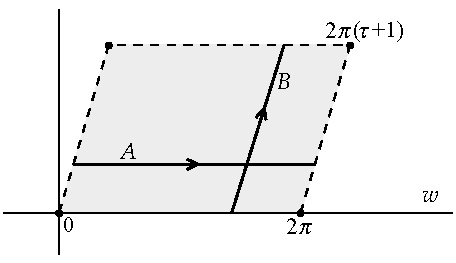
\includegraphics[width=0.8\linewidth]{figures/fig_5_1.pdf}
\caption{ゲージ $ds^2=dw\,d\bar w$ での、モジュラス $\tau$ をもつトーラス。上下の辺が同一視され、同様に左右の辺も同一視される。閉曲線 $A,B$ は、後で参照するために示してある。}
\label{fig:5.1}
\end{figure}

これを見るため、3.3節の局所的な議論で用いた手順を繰り返す。まず $2\nabla^2\omega=R$ を満たす Weyl 変換によって、計量を平坦にできる。$\nabla^2$ の固有モードで展開すると、周期境界条件の下では、$\omega$ に定数を加える自由を除いて一意な解が存在することがわかる。ここでは、Euler 数の $4\pi$ 倍である $\int d^2\sigma\,g^{1/2}R$ が、トーラスではゼロになることが重要である。続いて新しい座標 $\tilde\sigma^a$ に変換すれば、計量を単位計量の形にできる。しかし、点粒子の場合と同様、これが元の周期性を保つ保証はない。むしろ、今度は一般の並進 $u^a,v^a$ に対して、
\begin{equation}
\tilde\sigma^a\cong\tilde\sigma^a+2\pi(mu^a+nv^a)
\tag{5.1.10}\label{eq:5.1.10}
\end{equation}
となりうる。座標系を回転し、スケールを変え、それと同時に、計量の規格化を保つため $\omega$ をずらすことで、常に $u=(1,0)$ とおける。すると、$v$ の二つの成分という二つのパラメータが残る。$w=\tilde\sigma^1+i\tilde\sigma^2$ と定義すると、計量は $dw\,d\bar w$ で、周期性は
\begin{equation}
w\cong w+2\pi(m+n\tau)
\tag{5.1.11}\label{eq:5.1.11}
\end{equation}
となる。ここで $\tau=v^1+iv^2$ である。トーラスは、図\hyperref[fig:5.1]{5.1}に示すような、周期境界条件をもつ $w$ 平面内の平行四辺形である。

別の方法として、$w=\sigma^1+\tau\sigma^2$ によって $\sigma^a$ を定義しよう。元の周期性\hyperref[eq:5.1.8]{(5.1.8)}は保たれるが、計量は今度は、より一般的な形\hyperref[eq:5.1.9]{(5.1.9)}をとる。計量についての積分は、$\tau$ の実部と虚部についての二つの通常の積分に帰着する。計量\hyperref[eq:5.1.9]{(5.1.9)}は $\tau$ の複素共役に対して不変であり、$\tau$ が実数のとき退化するため、$\operatorname{Im}\tau>0$ に注意を限ることができる。円の\hyperref[eq:5.1.5a]{(5.1.5)}の場合と同様、これらのパラメータは、計量\hyperref[eq:5.1.9]{(5.1.9)}にも周期性\hyperref[eq:5.1.11]{(5.1.11)}にも入れられる。パラメータ $\tau$ は Teichmüller パラメータ、より一般的にはモジュラスと呼ばれる。点粒子の場合と異なるのは、円の不変な長さに類する、$\tau$ の簡単な不変表式がないことである。

点粒子の場合には対応物のない、追加の冗長性がいくらかある。$\tau+1$ という値は、$(m,n)\to(m-n,n)$ と置き換えることで、$\tau$ と同じ同一視の集合\hyperref[eq:5.1.11]{(5.1.11)}を生成する。$-1/\tau$ も、$w'=\tau w$ と定義して $(m,n)\to(n,-m)$ と置き換えれば同様である。これら二つの変換
\begin{equation}
T:\ \tau'=\tau+1,\qquad S:\ \tau'=-1/\tau
\tag{5.1.12}\label{eq:5.1.12}
\end{equation}
を繰り返し適用すると、$ad-bc=1$ を満たす任意の整数 $a,b,c,d$ に対する
\begin{equation}
\tau'=\frac{a\tau+b}{c\tau+d}
\tag{5.1.13}\label{eq:5.1.13}
\end{equation}
が生成される。

これは、次のようにも考えられる。変換
\begin{equation}
\begin{bmatrix}\sigma^1\\ \sigma^2\end{bmatrix}
=\begin{bmatrix}d&b\\c&a\end{bmatrix}
\begin{bmatrix}\sigma'^1\\ \sigma'^2\end{bmatrix}
\tag{5.1.14}\label{eq:5.1.14}
\end{equation}
は、$\sigma$ における計量\hyperref[eq:5.1.9]{(5.1.9)}を、$\sigma'$ における同じ形で、モジュラスが $\tau'$ となる計量に移す。これはトーラスの微分同相変換である。$ad-bc=1$ の帰結として一対一であり、周期性\hyperref[eq:5.1.8]{(5.1.8)}を保つ。しかし、無限小変換を順次行うことによって恒等変換から得ることはできない。いわゆる大きな座標変換である。座標 $\sigma$ での曲線 $A$ は、座標 $\sigma'$ では $A'$ 方向に $a$ 回、$B'$ 方向に $-c$ 回巡る曲線へ写る。これらの大きな座標変換は、行列式1の整数値 $2\times2$ 行列からなる群 $SL(2,\mathbb Z)$ をなす。$\tau$ 平面上の群は $SL(2,\mathbb Z)/\mathbb Z_2=PSL(2,\mathbb Z)$ である。$a,b,c,d$ の符号をすべて逆にしても、$\tau'$ は変わらないからである。変換\hyperref[eq:5.1.14]{(5.1.14)}の群は、モジュラー群と呼ばれる。

モジュラー変換\hyperref[eq:5.1.13]{(5.1.13)}を用いると、任意の $\tau$ が、図\hyperref[fig:5.2]{5.2}に示す領域 $F_0$、
\begin{equation}
-\frac12\leq\operatorname{Re}\tau\leq\frac12,\qquad |\tau|\geq1
\tag{5.1.15}\label{eq:5.1.15}
\end{equation}
の中のちょうど一点と等価であることを示せる。ただし、図のように同一視される境界は例外である。これは、上半平面を $PSL(2,\mathbb Z)$ で割った空間の基本領域と呼ばれる。同一視があるため、$F_0$ は巻き上げられ、$\operatorname{Im}\tau\to\infty$ のところだけが開いていると考えるべきである。基本領域 $F_0$ は、$(\mathrm{diff}\times\mathrm{Weyl})$ 非等価な計量のモジュライ空間の一つの表示である。

\begin{figure}[htbp]
\centering
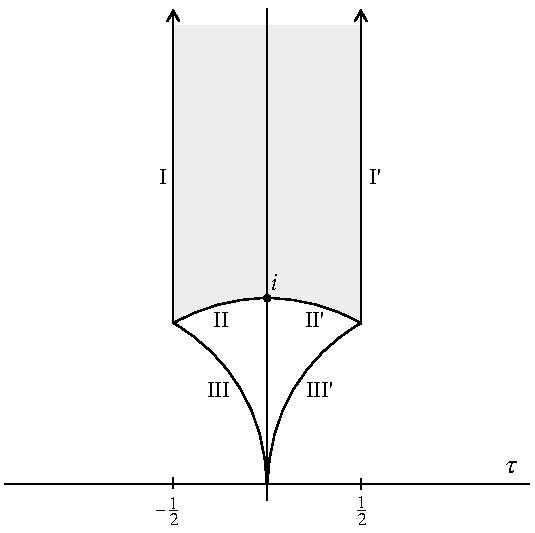
\includegraphics[width=0.8\linewidth]{figures/fig_5_2.pdf}
\caption{トーラスのモジュライ空間の標準的な基本領域 $F_0$。陰を付けて示してある。直線 I と I$'$ が同一視され、弧 II と II$'$ も同一視される。II、II$'$、III、III$'$ に囲まれた別の基本領域は、モジュラー変換 $S$ によって $F_0$ へ写される。}
\label{fig:5.2}
\end{figure}

点粒子の場合と同様、さらに厄介な点がある。$\tau$ が与えられた基本領域内にあり、計量が\hyperref[eq:5.1.9]{(5.1.9)}の形になることを要求しても、$\mathrm{diff}\times\mathrm{Weyl}$ 不変性のすべては固定されない。計量と周期性は、一様な並進
\begin{equation}
\sigma^a\longrightarrow\sigma^a+v^a
\tag{5.1.16}\label{eq:5.1.16}
\end{equation}
によって不変に保たれるので、$\mathrm{diff}\times\mathrm{Weyl}$ のこの二パラメータ部分群は固定されない。さらに、離散変換 $\sigma^a\to-\sigma^a$ も計量を不変にし、向き付けのない場合には、$\tau\to-\bar\tau$ を伴う $(\sigma^1,\sigma^2)\to(-\sigma^1,\sigma^2)$ もそうである。したがって、ここでも計量の自由度と局所対称性の間に二種類の不一致がある。対称性で取り除けない計量のパラメータと、計量の選択によって固定されない対称性である。固定されずに残る対称性は、共形 Killing 群（CKG）と呼ばれる。

振幅に十分な数の頂点演算子があれば、頂点演算子の位置のいくつかを固定することで、ゲージ不変性を完全に固定できる。$n$ 個の頂点演算子をもつトーラスでは、不変性\hyperref[eq:5.1.16]{(5.1.16)}を使って一つの頂点演算子の位置を固定でき、$\tau$ と残り $n-1$ 個の位置についての積分が残る。$\sigma^a\to-\sigma^a$ に由来する $\mathbb Z_2$ は、第二の頂点演算子をトーラスの半分に制限すれば固定できる。実際には、有限の重複計数については、一部の対称性を固定せずに残し、適切な因子で割る方が便利なことが多い。また、頂点演算子の数が少なすぎると、共形 Killing 不変性の一部が固定されずに残るので、その重複計数を明示的に考慮しなければならない。

\subsubsectionlink*{読者への注意}

この章の残りでは、モジュライをより一般的に論じ、ゲージ固定した積分の測度を求める。主な目標は、弦の $S$ 行列のゲージ固定した表式\hyperref[eq:5.3.9]{(5.3.9)}である。実際、弦の興味深い物理の大部分は、木のレベルと1ループの振幅で見ることができる。これらについては、近道を用いて測度を得られる。木のレベルの振幅には計量のモジュライはないが、いくつかの頂点演算子の位置を固定しなければならない。その測度は、式(6.4.4)の後で説明するように推定できる。1ループ振幅の測度は、式(7.3.9)の後の点粒子の測度の議論との類推から、かなり直観的に理解できる。したがって、読者はこの章の残りを飛ばしてもよい（あるいは、式\hyperref[eq:5.3.9]{(5.3.9)}までざっと読んでもよい）。また、Faddeev--Popov ゴーストを扱うすべての節を飛ばすこともできる。

\subsectionlink{モジュライとRiemann面}\label{sec:5.2}

前の議論を、より一般的かつ抽象的な形で繰り返そう。与えられた位相型 $r$ 上のすべての計量についての積分から出発する。計量の空間を $\mathcal G_r$ と呼ぶ。向き付けられた閉曲面では、$r$ は取っ手の数、すなわち種数 $g$ だけで指定できる。$\mathrm{diff}\times\mathrm{Weyl}$ の冗長性を考慮すると、モジュライ空間
\begin{equation}
\mathcal M_r=\frac{\mathcal G_r}{(\mathrm{diff}\times\mathrm{Weyl})_r}
\tag{5.2.1}\label{eq:5.2.1}
\end{equation}
が残る。トーラスの場合と同様、この空間は有限個のモジュライによってパラメータ付けられる。トーラスでは、$\mathcal M_1$ は上半平面を $PSL(2,\mathbb Z)$ で割った空間、あるいは等価的に、$F_0$ など任意の基本領域である。また、計量を不変にする $\mathrm{diff}\times\mathrm{Weyl}$ の部分群 CKG が存在する場合もある。

経路積分に頂点演算子があるときには、その位置を計量に由来するモジュライと同等に扱い、すべてをモジュライと呼ぶと便利である。区別が必要なときには、計量のモジュライと明示する。経路積分に頂点演算子がある場合に使える、CKG への対処法の一つは、一部の頂点演算子の座標を固定してゲージをさらに指定することである。Polyakov 経路積分には、$\mathcal G_r$ 上の積分と、$n$ 個の頂点演算子の位置を世界面 $M$ 上で積分するものが含まれる。したがって、位相型 $r$ で $n$ 個の頂点演算子をもつ場合のモジュライ空間は
\begin{equation}
\mathcal M_{r,n}
=\frac{\mathcal G_r\times M^n}{(\mathrm{diff}\times\mathrm{Weyl})_r}
\tag{5.2.2}\label{eq:5.2.2}
\end{equation}
である。

トーラスについて見たように、$\mathrm{diff}_r$ は一般には連結でない。恒等変換を含む連結成分 $\mathrm{diff}_{r0}$ を取り出すと、商
\begin{equation}
\frac{\mathrm{diff}_r}{\mathrm{diff}_{r0}}
\tag{5.2.3}\label{eq:5.2.3}
\end{equation}
がモジュラー群である。

計量の $\mathrm{diff}\times\mathrm{Weyl}$ 冗長性を無限小の水準で調べると興味深い。すなわち、$\mathrm{diff}\times\mathrm{Weyl}$ 変換と等価でなく、したがってモジュライの変化に対応する、小さな計量の変分を探す。また、計量を変えない小さな $\mathrm{diff}\times\mathrm{Weyl}$ 変換も探す。これらは CKG の無限小要素であり、共形 Killing ベクトル（CKV）と呼ばれる。このことから、モジュライと CKG の起源をさらに理解できる。

無限小 $\mathrm{diff}\times\mathrm{Weyl}$ 変換は、計量を
\begin{equation}
\delta g_{ab}=-2(P_1\delta\sigma)_{ab}
+(2\delta\omega-\nabla\cdot\delta\sigma)g_{ab}
\tag{5.2.4}\label{eq:5.2.4}
\end{equation}
だけ変える。ここで $P_1$ は、微分のトレースレスな対称線形結合(3.3.17)である。モジュライは、すべての変分\hyperref[eq:5.2.4]{(5.2.4)}に直交する計量の変分 $\delta'g_{ab}$ に対応する。
\begin{equation}
\begin{aligned}
0&=\int d^2\sigma\,g^{1/2}\delta'g_{ab}
\left[-2(P_1\delta\sigma)^{ab}
+(2\delta\omega-\nabla\cdot\delta\sigma)g^{ab}\right]\\
&=\int d^2\sigma\,g^{1/2}
\left[-2(P_1^T\delta'g)_a\delta\sigma^a
+\delta'g_{ab}g^{ab}(2\delta\omega-\nabla\cdot\delta\sigma)\right].
\end{aligned}
\tag{5.2.5}\label{eq:5.2.5}
\end{equation}
転置 $(P_1^Tu)_a=-\nabla^bu_{ab}$ は、演習3.2と同じように定義する。一般の $\delta\omega,\delta\sigma$ に対して内積\hyperref[eq:5.2.5]{(5.2.5)}がゼロになるには、
\begin{align}
g^{ab}\delta'g_{ab}&=0,
\tag{5.2.6a}\label{eq:5.2.6a}\\
(P_1^T\delta'g)_a&=0
\tag{5.2.6b}\label{eq:5.2.6b}
\end{align}
が必要である。第一の条件は、$\delta'g_{ab}$ のトレースがゼロであることを要求する。$P_1^T$ が作用するのは、このトレースレス対称テンソルである。これらの方程式の各解に対して、一つのモジュラスが存在する。

CKV は、$\delta g_{ab}=0$ となる変換\hyperref[eq:5.2.4]{(5.2.4)}である。この方程式のトレースは $\delta\omega$ を一意に固定し、共形 Killing 方程式
\begin{equation}
(P_1\delta\sigma)_{ab}=0
\tag{5.2.7}\label{eq:5.2.7}
\end{equation}
が残る。

共形ゲージの周りの変分に対しては、式\hyperref[eq:5.2.6a]{(5.2.6)}と\hyperref[eq:5.2.7]{(5.2.7)}は簡単になる。
\begin{align}
\partial_{\bar z}\delta'g_{zz}
&=\partial_z\delta'g_{\bar z\bar z}=0,
\tag{5.2.8a}\label{eq:5.2.8a}\\
\partial_{\bar z}\delta z&=\partial_z\delta\bar z=0.
\tag{5.2.8b}\label{eq:5.2.8b}
\end{align}
したがって、モジュライの変分は正則二次微分に、CKV は正則ベクトル場に対応する。トーラス上で正則かつ二重周期的な関数は定数だけなので、実モジュライが二つ、実 CKV が二つあり、前節の議論と一致する。

計量のモジュライは $P_1^T$ の核\hyperref[eq:5.2.6a]{(5.2.6)}に、CKV は $P_1$ の核\hyperref[eq:5.2.7]{(5.2.7)}に対応する。Riemann--Roch の定理は、計量のモジュライの数 $\mu=\dim\ker P_1^T$ と CKV の数 $\kappa=\dim\ker P_1$ を、Euler 数 $\chi$ に関係づける。
\begin{equation}
\mu-\kappa=-3\chi.
\tag{5.2.9}\label{eq:5.2.9}
\end{equation}
これは、この章の後で導くことができる。向き付けられた閉曲面では、$-3\chi=6g-6$ である。この数え方は実モジュライについてのものであり、$\tau$ のような複素モジュラスは実部と虚部に分けて数える。

さらに、$\chi<0$ では $\kappa$ がゼロとなり、$\chi>0$ では $\mu$ がゼロとなる。これを示すため、まず、Weyl 変換によってスカラー曲率 $R$ が一定になる計量を常に見いだせるという事実を用いる。このとき、$R$ の符号は $\chi$ の符号と同じである。$P_1^TP_1=-\tfrac12\nabla^2-\tfrac14R$ なので、
\begin{equation}
\begin{aligned}
\int d^2\sigma\,g^{1/2}
(P_1\delta\sigma)_{ab}(P_1\delta\sigma)^{ab}
&=\int d^2\sigma\,g^{1/2}
\delta\sigma_a(P_1^TP_1\delta\sigma)^a\\
&=\int d^2\sigma\,g^{1/2}
\left(\frac12\nabla_a\delta\sigma_b\nabla^a\delta\sigma^b
-\frac R4\delta\sigma_a\delta\sigma^a\right).
\end{aligned}
\tag{5.2.10}\label{eq:5.2.10}
\end{equation}
$\chi$ が負の場合、右辺は厳密に正なので、$P_1\delta\sigma$ はゼロになれない。同様の議論によって、$\chi$ が正の場合には $P_1^T\delta'g$ がゼロになれないことが示される。これらの結果を組み合わせると、
\begin{align}
\chi>0:&\qquad \kappa=3\chi,\quad\mu=0,
\tag{5.2.11a}\label{eq:5.2.11a}\\
\chi<0:&\qquad \kappa=0,\quad\mu=-3\chi
\tag{5.2.11b}\label{eq:5.2.11b}
\end{align}
を得る。

\subsubsectionlink*{Riemann面}

モジュライ空間を記述する馴染み深い方法は、各同値類から一つの計量を選ぶことである。これは、モジュライ $t^k$ に依存する計量の族 $\hat g_{ab}(t;\sigma)$ となる。トーラスでは、式\hyperref[eq:5.1.9]{(5.1.9)}がそのような切片を与える。計量 $dw\,d\bar w$ を固定し、モジュライを座標領域に組み込む\hyperref[eq:5.1.11]{(5.1.11)}の形の別の記述を用いると、しばしば便利である。この考えは、次のように形式化できる。

まず、可微分多様体の定義を思い出そう。多様体を、互いに重なり合うパッチの集合で覆い、第 $m$ パッチには座標 $\sigma_m^a$ を与える。$a$ は1から多様体の次元までの値をとる。パッチ $m,n$ が重なるとき、その二つのパッチの座標は
\begin{equation}
\sigma_m^a=f_{mn}^a(\sigma_n)
\tag{5.2.12}\label{eq:5.2.12}
\end{equation}
によって関係づけられ、遷移関数 $f_{mn}$ には、指定された回数だけ微分可能であることを要求する。Riemann 多様体では、各パッチに計量 $g_{m,ab}(\sigma_m)$ も与えられ、重なりでの値は通常のテンソル変換則によって関係づけられる。

複素多様体では、各パッチに複素座標 $z_m^a$ があり、今度は $a$ が1から多様体の次元の半分まで動く。遷移関数は正則であることを要求する。
\begin{equation}
z_m^a=f_{mn}^a(z_n).
\tag{5.2.13}\label{eq:5.2.13}
\end{equation}
正則性はどの座標 $z_m^a$ を使うかに依存しないので、多様体上の正則関数を定義できる。二つの可微分多様体の間に一対一の可微分写像があればそれらが等価であるのと同様に、二つの複素多様体の間に一対一の正則写像があれば、それらは等価である。とくに、各パッチの内部で正則な座標変換を行うと、等価な曲面が得られる。

二次元、すなわち複素座標が一つの場合、複素多様体は Riemann面と呼ばれる。この場合、一対一対応
\begin{equation}
\text{Riemann面}\quad\longleftrightarrow\quad
\text{Riemann 多様体を Weyl 変換で割ったもの}
\tag{5.2.14}\label{eq:5.2.14}
\end{equation}
がある。右辺で「Weyl 変換で割る」とだけしたのは、「微分同相変換で割る」ことがすでに Riemann 多様体の定義に暗黙に含まれるからである。この同型を見るため、Riemann 多様体から出発しよう。共形ゲージの議論から、各座標パッチ内に、
\begin{equation}
ds^2\propto dz_m\,d\bar z_m
\tag{5.2.15}\label{eq:5.2.15}
\end{equation}
を満たす座標 $z_m$ を見つけられることがわかっている。隣接するパッチでは座標が同じである必要はないが、$ds^2\propto dz_m\,d\bar z_m\propto dz_n\,d\bar z_n$ なので、遷移関数は正則となる。\footnote[1]{正確には、反正則な遷移関数も可能である。向き付けられた弦では、標準の向きを選ぶことでこれを禁止する。向き付けのない弦では許される。厳密な意味での Riemann面は、境界をもたない向き付けられた多様体を指す。}
これが、実二次元における Riemann 多様体から複素多様体への写像である。逆写像については、第 $m$ パッチの計量を $dz_m\,d\bar z_m$ とし、重なりで滑らかにつなぐことで（これは1の分割という標準的な構成である）、Riemann 多様体を作れる。したがって、Riemann面の二つの特徴づけは等価である。

平行四辺形（図\hyperref[fig:5.1]{5.1}）の複素座標 $w$ によるトーラスの記述は、複素多様体という考えを具体的に示している。図\hyperref[fig:5.1]{5.1}の基本平行四辺形より少し大きい一つの座標パッチをとると考えよう。周期性の条件
\begin{equation}
w\cong w+2\pi\cong w+2\pi\tau
\tag{5.2.16}\label{eq:5.2.16}
\end{equation}
は、そのパッチの向かい合う辺の重なりにおける遷移関数となる。曲面は、これらの遷移関数によって定義される。元の計量についての経路積分を定義するには、まず計量を、正方形\hyperref[eq:5.1.7]{(5.1.7)}のような固定座標上の関数、あるいは少なくとも、固定した遷移関数をもつ固定した座標パッチの集合上の関数とみなすのが最も簡単である。その後、与えられた曲面上の場の量子論を調べるには、平行四辺形\hyperref[eq:5.1.11]{(5.1.11)}のように、単位計量と、モジュライに依存する遷移関数を用いるのが最も容易である。

Riemann面は、次のようにも考えられる。世界面をパッチの和集合として定義し、$\mathrm{diff}\times\mathrm{Weyl}$ の自由を用いて、各パッチで計量を $dz\,d\bar z$ にできる。すると、重なり合うパッチでのゲージの選択は、この計量を不変にする $\mathrm{diff}\times\mathrm{Weyl}$ 変換によってのみ異なりうる。すでに議論したように、これらは共形変換である。したがって Riemann面は、CFT が定義される自然な場所である。CFT の場は、共形変換の下で確定した変換性をもつからである。

\subsectionlink{モジュライの測度}\label{sec:5.3}

ここで、Polyakov 経路積分のゲージ固定を再び考える。ゲージ冗長性は、計量についての経路積分を完全には取り除かず、モジュライ空間上の有限次元積分を残すことを学んだ。これを考慮するために、3.3節の議論を精密化する必要がある。

$S$ 行列の Polyakov 経路積分は
\begin{equation}
\begin{aligned}
S_{j_1\cdots j_n}(k_1,\ldots,k_n)
={}&\sum_{\substack{\text{コンパクトな}\\\text{位相型}}}
\int\frac{[d\phi\,dg]}{V_{\mathrm{diff}\times\mathrm{Weyl}}}
\exp(-S_{\mathrm m}-\lambda\chi)\\
&\quad\times\prod_{i=1}^n
\int d^2\sigma_i\,g(\sigma_i)^{1/2}
\mathcal V_{j_i}(k_i,\sigma_i)
\end{aligned}
\tag{5.3.1}\label{eq:5.3.1}
\end{equation}
である。これは以前の表式\hyperref[eq:3.5.5]{(3.5.5)}だが、今度は一般の $c=\tilde c=26$ の物質理論を用いて書き、物質場を $\phi$ と表している。ゲージ固定では、計量と位置についての積分を、ゲージ群、モジュライ、固定されていない位置についての積分に変換する。
\begin{equation}
[dg]\,d^{2n}\sigma\longrightarrow[d\zeta]\,d^\mu t\,d^{2n-\kappa}\sigma.
\tag{5.3.2}\label{eq:5.3.2}
\end{equation}
ゲージ群の体積を分離して除いた後、この変換の Jacobian がモジュライ空間上の測度となる。

手順は3.3節と同じだが、今度はモジュライと CKV を考慮する。とくに、ゲージの選択は、頂点演算子の座標のうち $\kappa$ 個を $\sigma_i^a\to\hat\sigma_i^a$ と固定することになる。固定された座標 $(a,i)$ の集合を $f$ と表す。モジュライ空間上の Faddeev--Popov 測度を
\begin{equation}
1=\Delta_{\mathrm{FP}}(g,\sigma)
\int_Fd^\mu t\int_{\mathrm{diff}\times\mathrm{Weyl}}[d\zeta]\,
\delta\bigl(g-\hat g(t)^\zeta\bigr)
\prod_{(a,i)\in f}\delta\bigl(\sigma_i^a-\hat\sigma_i^{\zeta a}\bigr)
\tag{5.3.3}\label{eq:5.3.3}
\end{equation}
によって定義する。定義により、すべての計量は、少なくとも一組の $t,\zeta$ の値について $\hat g(t)$ と $(\mathrm{diff}\times\mathrm{Weyl})$ 等価である。固定座標のデルタ関数は、そこから一意の $\zeta$ を選び出す。ただし、5.1節の最後で述べたように、位数が有限の $n_R$ である離散対称群が残る場合がある。その場合、デルタ関数は $n_R$ 個の点でゼロでなくなる。

表式\hyperref[eq:5.3.3]{(5.3.3)}を経路積分\hyperref[eq:5.3.1]{(5.3.1)}に挿入し、以前と同じ手順を踏むと、
\begin{equation}
\begin{aligned}
S_{j_1\cdots j_n}(k_1,\ldots,k_n)
={}&\sum_{\substack{\text{コンパクトな}\\\text{位相型}}}
\int_Fd^\mu t\,\Delta_{\mathrm{FP}}\bigl(\hat g(t),\hat\sigma\bigr)
\int[d\phi]\int\prod_{(a,i)\notin f}d\sigma_i^a\\
&\quad\times\exp\bigl(-S_{\mathrm m}[\phi,\hat g(t)]-\lambda\chi\bigr)
\prod_{i=1}^n\left[\hat g(\sigma_i)^{1/2}
\mathcal V_{j_i}(k_i;\sigma_i)\right]
\end{aligned}
\tag{5.3.4}\label{eq:5.3.4}
\end{equation}
を得る。計量と頂点演算子の座標についての積分は、計量のモジュライ空間 $F$ と固定されていない座標についての積分に帰着し、その測度は $\Delta_{\mathrm{FP}}$ によって与えられている。頂点演算子では、位置のうち $\kappa$ 個が固定されている。

次に、Faddeev--Popov 測度を評価する。デルタ関数は、対称性で関係づけられた $n_R$ 個の点でゼロでないため、そのうちの一点を考え、$n_R$ で割る。その点の近くで、$\Delta_{\mathrm{FP}}$ の定義\hyperref[eq:5.3.3]{(5.3.3)}を展開する。一般の計量の変分は、局所対称変換による変分とモジュライ $t^k$ の変化との和に等しい。
\begin{equation}
\delta g_{ab}
=\sum_{k=1}^{\mu}\delta t^k\partial_{t^k}\hat g_{ab}
-2(\hat P_1\delta\sigma)_{ab}
+(2\delta\omega-\hat\nabla\cdot\delta\sigma)\hat g_{ab}.
\tag{5.3.5}\label{eq:5.3.5}
\end{equation}
すると、Faddeev--Popov 行列式の逆数は
\begin{equation}
\begin{aligned}
\Delta_{\mathrm{FP}}(\hat g,\hat\sigma)^{-1}
&=n_R\int d^\mu\delta t\,[d\delta\omega\,d\delta\sigma]\,
\delta(\delta g_{ab})
\prod_{(a,i)\in f}\delta\bigl(\delta\sigma^a(\hat\sigma_i)\bigr)\\
&=n_R\int d^\mu\delta t\,d^\kappa x\,[d\beta'\,d\delta\sigma]\\
&\quad\times\exp\left[
2\pi i(\beta',2\hat P_1\delta\sigma-\delta t^k\partial_k\hat g)
+2\pi i\sum_{(a,i)\in f}x_{ai}\delta\sigma^a(\hat\sigma_i)
\right].
\end{aligned}
\tag{5.3.6}\label{eq:5.3.6}
\end{equation}
第二の表式の内積は、演習3.2で定義したものである。3.3節の局所的な議論と同じ手順に従い、デルタ関数とデルタ汎関数を $x$ と $\beta_{ab}$ の積分として書き、その後 $\delta\omega$ を積分して、$\beta'_{ab}$ のトレースがゼロであるという制約を得た。

以前と同じく、すべてのボソン変数を Grassmann 変数に置き換えることで、積分\hyperref[eq:5.3.6]{(5.3.6)}の逆数をとる。
\begin{align}
\delta\sigma^a&\longrightarrow c^a,
\tag{5.3.7a}\label{eq:5.3.7a}\\
\beta'_{ab}&\longrightarrow b_{ab},
\tag{5.3.7b}\label{eq:5.3.7b}\\
x_{ai}&\longrightarrow\eta_{ai},
\tag{5.3.7c}\label{eq:5.3.7c}\\
\delta t^k&\longrightarrow\xi^k.
\tag{5.3.7d}\label{eq:5.3.7d}
\end{align}
すると、場を便利に規格化すれば、
\begin{equation}
\begin{aligned}
\Delta_{\mathrm{FP}}(\hat g,\hat\sigma)
&=\frac1{n_R}\int[db\,dc]\,d^\mu\xi\,d^\kappa\eta\\
&\quad\times\exp\left[
-\frac1{4\pi}(b,2\hat P_1c-\xi^k\partial_k\hat g)
+\sum_{(a,i)\in f}\eta_{ai}c^a(\hat\sigma_i)\right]\\
&=\frac1{n_R}\int[db\,dc]\exp(-S_{\mathrm g})
\prod_{k=1}^{\mu}\frac1{4\pi}(b,\partial_k\hat g)
\prod_{(a,i)\in f}c^a(\hat\sigma_i).
\end{aligned}
\tag{5.3.8}\label{eq:5.3.8}
\end{equation}
最後の行では、Grassmann パラメータ $\eta_{ai},\xi^k$ を積分した。

モジュライ空間上の積分に適した測度は、挿入を伴うこのゴースト経路積分によって生成される。途中の段階で全体の符号を追跡することはしない。これは Jacobian であるべきものなので、正の結果を与えるように全体の符号を暗黙に選ぶ。その結果、$S$ 行列の完全な表式は
\begin{equation}
\begin{aligned}
S_{j_1\cdots j_n}(k_1,\ldots,k_n)
={}&\sum_{\substack{\text{コンパクトな}\\\text{位相型}}}
\int_F\frac{d^\mu t}{n_R}
\int[d\phi\,db\,dc]\exp(-S_{\mathrm m}-S_{\mathrm g}-\lambda\chi)\\
&\times\prod_{(a,i)\notin f}\int d\sigma_i^a\,
\prod_{k=1}^{\mu}\frac1{4\pi}(b,\partial_k\hat g)\\
&\times\prod_{(a,i)\in f}c^a(\hat\sigma_i)\,
\prod_{i=1}^n\hat g(\sigma_i)^{1/2}\mathcal V_{j_i}(k_i,\sigma_i)
\end{aligned}
\tag{5.3.9}\label{eq:5.3.9}
\end{equation}
となる。この結果は、閉弦と開弦、向き付けのあるものとないものという、すべてのボソン弦理論に容易に拡張できる。違いは、含まれる位相型と許される頂点演算子だけである。式\hyperref[eq:5.3.9]{(5.3.9)}は、有用で優美な結果である。モジュライと CKV に由来する複雑さは、経路積分の中の $c,b$ の挿入によって考慮される。固定座標ごとに $d\sigma_i^a$ が $c_i^a$ に置き換わり、各計量モジュラスは一つの $b$ の挿入を生じさせる。

\subsubsectionlink*{行列式による表式}

式\hyperref[eq:5.3.8]{(5.3.8)}では、Faddeev--Popov 行列式を、Grassmann パラメータと場についての積分で表した。ここでは、これを有限次元の行列式と汎関数行列式の積に帰着させる。後の章で弦の $S$ 行列を調べるとき、この直接的な経路積分によるアプローチは、用いる方法の一つとなる。

ゴースト場を適切な完全系で展開する。
\begin{equation}
c^a(\sigma)=\sum_Jc_JC_J^a(\sigma),\qquad
b_{ab}(\sigma)=\sum_Kb_KB_{Kab}(\sigma).
\tag{5.3.10}\label{eq:5.3.10}
\end{equation}
完全系 $C_J^a,B_{Kab}$ は、次のように定義する。ゴースト作用に現れる微分 $P_1$ は、ベクトルをトレースレス対称テンソルに移す。その転置は逆のことを行う。ゴースト作用は、どちらを用いても書ける。
\begin{equation}
S_{\mathrm g}=\frac1{2\pi}(b,P_1c)
=\frac1{2\pi}(P_1^Tb,c).
\tag{5.3.11}\label{eq:5.3.11}
\end{equation}
$P_1$ はある種類の場を別の種類の場に変えるため、微分同相不変な仕方で対角化することはできない。しかし、$P_1^TP_1$ と $P_1P_1^T$ は対角化できる。
\begin{equation}
P_1^TP_1C_J^a=\nu_J'^2C_J^a,\qquad
P_1P_1^TB_{Kab}=\nu_K^2B_{Kab}.
\tag{5.3.12}\label{eq:5.3.12}
\end{equation}
固有関数は実に選ぶことができ、それぞれの内積
\begin{align}
(C_J,C_{J'})
&=\int d^2\sigma\,g^{1/2}C_J^aC_{J'a}
=\delta_{JJ'},
\tag{5.3.13a}\label{eq:5.3.13a}\\
(B_K,B_{K'})
&=\int d^2\sigma\,g^{1/2}B_{Kab}B_{K'}^{ab}
=\delta_{KK'}
\tag{5.3.13b}\label{eq:5.3.13b}
\end{align}
によって規格化する。

ここで、
\begin{equation}
(P_1P_1^T)P_1C_J
=P_1(P_1^TP_1)C_J=\nu_J'^2P_1C_J
\tag{5.3.14}\label{eq:5.3.14}
\end{equation}
に注意しよう。したがって、$P_1C_J$ は $P_1P_1^T$ の固有関数である。同様に、$P_1^TB_K$ は $P_1^TP_1$ の固有関数である。よって、$P_1C_J=0$ または $P_1^TB_K=0$ の場合を除いて、固有関数の間には一対一対応がある。後者は、$P_1^TP_1$ または $P_1P_1^T$ のゼロ固有値に対応する。これらはまさに CKV と正則二次微分なので、その数はそれぞれ $\kappa,\mu$ である。固有値ゼロの固有関数は $C_{0j},B_{0k}$ と表し、ゼロでない固有値には $J,K=1,\ldots$ という添字を付けよう。後者については、規格化された固有関数の間に
\begin{equation}
B_{Jab}=\frac1{\nu_J}(P_1C_J)_{ab},\qquad
\nu_J=\nu'_J\ne0
\tag{5.3.15}\label{eq:5.3.15}
\end{equation}
という関係がある。

モードで書くと、ゴースト経路積分 $\Delta_{\mathrm{FP}}$ は
\begin{equation}
\begin{aligned}
&\int\prod_{k=1}^{\mu}db_{0k}
\prod_{j=1}^{\kappa}dc_{0j}
\prod_Jdb_J\,dc_J\,
\exp\left(-\frac{\nu_Jb_Jc_J}{2\pi}\right)\\
&\qquad\times\prod_{k'=1}^{\mu}\frac1{4\pi}(b,\partial_{k'}\hat g)
\prod_{(a,i)\in f}c^a(\sigma_i)
\end{aligned}
\tag{5.3.16}\label{eq:5.3.16}
\end{equation}
となる。A.2節によれば、Grassmann 積分は、積分変数が被積分関数に現れない限りゼロになる。$c_{0j},b_{0k}$ は作用には現れず、挿入の中にだけ現れる。実際、積分\hyperref[eq:5.3.16]{(5.3.16)}の中のそれぞれの種類の挿入の数 $\kappa,\mu$ は、対応するゴーストのゼロモードの数とちょうど一致する。ゼロでない答えを得るのに必要なだけの挿入がちょうどあり、挿入ではゴースト場のゼロモード部分だけが寄与する。したがって、
\begin{equation}
\begin{aligned}
\Delta_{\mathrm{FP}}
={}&\int\prod_{k=1}^{\mu}db_{0k}
\prod_{k'=1}^{\mu}\left[
\sum_{k''=1}^{\mu}\frac{b_{0k''}}{4\pi}
(B_{0k''},\partial_{k'}\hat g)\right]\\
&\times\int\prod_{j=1}^{\kappa}dc_{0j}
\prod_{(a,i)\in f}\left[
\sum_{j'=1}^{\kappa}c_{0j'}C_{0j'}^a(\sigma_i)\right]\\
&\times\int\prod_Jdb_J\,dc_J
\exp\left(-\frac{\nu_Jb_Jc_J}{2\pi}\right).
\end{aligned}
\tag{5.3.17}\label{eq:5.3.17}
\end{equation}
ゼロモード積分を Grassmann 変数で飽和させるすべての仕方について和をとると、それぞれで有限次元の行列式が生成される。一方、非ゼロモードは無限積、すなわち汎関数行列式を与える。全体として、
\begin{equation}
\Delta_{\mathrm{FP}}
=\det\frac{(B_{0k},\partial_{k'}\hat g)}{4\pi}\,
\det C_{0j}^a(\sigma_i)\,
\left[\det{}'\left(\frac{P_1^TP_1}{4\pi^2}\right)\right]^{1/2}.
\tag{5.3.18}\label{eq:5.3.18}
\end{equation}
$C_{0j}^a(\sigma_i)$ が正方行列であることに注意しよう。$(a,i)\in f$ がとる値は、$j$ と同じく $\kappa$ 個である。汎関数行列式のプライムは、ゼロ固有値を除くことを表す。

\subsubsectionlink*{Riemann--Roch の定理}

これで、Riemann--Roch の定理を経路積分から導くことができる。正則な $bc$ 系（$\tilde b,\tilde c$ を含まない）のゴーストカレントについて、演習3.6で導いたカレント保存則の異常は
\begin{equation}
\nabla_aj^a=\frac{1-2\lambda}{4}R
\tag{5.3.19}\label{eq:5.3.19}
\end{equation}
である。

Noether の定理は、保存カレントを不変性に関係づける。保存しないカレントについても同じ議論を行うと、
\begin{equation}
\frac{\delta\bigl([d\phi]\exp(-S)\bigr)}
{[d\phi]\exp(-S)}
=\frac{i\epsilon}{2\pi}\int d^2\sigma\,g^{1/2}\nabla_aj^a
\longrightarrow-i\epsilon\frac{2\lambda-1}{2}\chi
\tag{5.3.20}\label{eq:5.3.20}
\end{equation}
が得られる。ゴースト数の対称性は $\delta b=-i\epsilon b$、$\delta c=i\epsilon c$ と作用する。経路積分がゼロでないとき、測度、作用、挿入の変換は相殺しなければならない。したがって、異常から、$c$ の挿入の数から $b$ の挿入の数を引いたものは $3\chi/2$ であるとわかる。経路積分の計算は、挿入の数をゼロモードの数に関係づけるので、同じ差に対して
\begin{equation}
\frac12(\kappa-\mu)
=\frac12(\dim\ker P_1-\dim\ker P_1^T)
\tag{5.3.21}\label{eq:5.3.21}
\end{equation}
を与える。因子 $\tfrac12$ が現れるのは、正則な理論だけをとったからである。反正則な理論は同じ寄与を与える。異常から得た結果とゼロモードから得た結果を等置すれば、Riemann--Roch の定理 $\kappa-\mu=3\chi$ が得られる。一般の $bc$ 系についても、同じように
\begin{equation}
\dim\ker P_n-\dim\ker P_n^T=(2n+1)\chi
\tag{5.3.22}\label{eq:5.3.22}
\end{equation}
が得られる。これらの演算子は演習3.2で定義されている。

\subsectionlink{測度についての補足}

ここでは、ゲージ固定した弦の振幅の一般的な性質をいくつかまとめる。これらは主として、第9章の、より形式的な考察に役立つ。

\subsubsectionlink*{ゲージ不変性}

Faddeev--Popov の手続きによって、ゲージ固定した振幅が BRST 不変であり、ゲージの選び方に依存しないことは保証されている。しかし、期待される不変性をすべて備えていることを明示的に確かめておくのは有用である。第一に、振幅はモジュライ空間上の座標 $t$ の選び方に依存しない。新しい座標 $t'{}^k(t)$ に対して、
\begin{equation}
\begin{aligned}
d^\mu t'&=\left|\det\frac{\partial t'}{\partial t}\right|d^\mu t,\\
\prod_{k=1}^{\mu}\frac{1}{4\pi}(b,\partial'_k\hat g)
&=\det\left(\frac{\partial t}{\partial t'}\right)
\prod_{k=1}^{\mu}\frac{1}{4\pi}(b,\partial_k\hat g)
\end{aligned}
\tag{5.4.1}\label{eq:5.4.1}
\end{equation}
となり、二つの Jacobian は相殺する（符号を除く。この符号は、すでに述べたように、測度が正になるよう手で定めなければならない）。言い換えると、$b$ ゴーストの挿入によって、被積分関数はモジュライ空間上の密度として変換する。

第二に、測度がゲージ切片の Weyl 変換のもとで不変であることを見よう。Weyl 変換
\begin{equation}
\delta\hat g'_{ab}(t;\sigma)
=2\delta\omega(t;\sigma)\hat g_{ab}(t;\sigma)
\tag{5.4.2}\label{eq:5.4.2}
\end{equation}
のもとで、作用と測度の変分は局所演算子 $T^a{}_a$ の挿入を与える。これは $D=26$ では運動方程式によって消える。したがって、さまざまな挿入への影響だけを考えればよい。頂点演算子の挿入は、その構成から Weyl 不変である。$c^a(\sigma_i)$ の挿入は、式(3.3.24)の下で議論したように Weyl 不変である。$b$ の挿入については、
\begin{equation}
\begin{aligned}
(b,\partial_k\hat g')
&=\int d^2\sigma\,\hat g'{}^{1/2}b_{ab}
\hat g'{}^{ac}\hat g'{}^{bd}\partial_k\hat g'_{cd}\\
&=\int d^2\sigma\,\hat g^{1/2}b_{ab}
\left(\hat g^{ac}\hat g^{bd}\partial_k\hat g_{cd}
+2\hat g^{ab}\partial_k\omega\right)\\
&=(b,\partial_k\hat g)
\end{aligned}
\tag{5.4.3}\label{eq:5.4.3}
\end{equation}
であり、最後の等式は $b$ がトレースレスであることによる。

第三に、無限小の diff 変換 $\delta\sigma=\xi(t;\sigma)$ のもとでの不変性を確かめよう。一般の diff 変換への拡張は容易である。振幅\hyperref[eq:5.3.9]{(5.3.9)}のうち、不変性がただちには明らかでない項は、$b$ の挿入と、座標が固定された頂点演算子だけである。前者は
\begin{equation}
\begin{aligned}
\delta(b,\partial_k\hat g)
&=-2(b,P_1\partial_k\xi)\\
&=-2(P_1^Tb,\partial_k\xi)\\
&=0
\end{aligned}
\tag{5.4.4}\label{eq:5.4.4}
\end{equation}
と変換する。ここでは $b$ の運動方程式を用いた。$b$ の運動方程式は $\delta S/\delta c=0$ から得られるので、$c$ の挿入の位置には源の項が現れる。これらは、固定された頂点演算子への座標変換の影響を取り込むために、まさに必要なものである。

\subsubsectionlink*{BRST 不変性}

次に、振幅\hyperref[eq:5.3.9]{(5.3.9)}の完全な BRST 不変性を確かめる。経路積分の測度と作用が不変であることは局所的な解析からわかっているので、挿入に対する BRST 変換の影響を考える必要がある。ゲージ固定した経路積分\hyperref[eq:5.3.9]{(5.3.9)}では、積分しない頂点演算子には $c$ または $\tilde c c$ の因子が伴う。これは、OCQ 状態に対応する BRST 不変な頂点演算子について、第4.4節の末尾で述べたものにほかならない。一方、積分する頂点演算子は BRST 不変ではないが、その BRST 変分が
\begin{equation}
\delta_B\mathcal V_{\mathrm m}
=i\epsilon\,\partial_a(c^a\mathcal V_{\mathrm m})
\tag{5.4.5}\label{eq:5.4.5}
\end{equation}
であることを示すのは演習とする。これは積分すれば消える。

最後に、$b$ の挿入の変分がある。
\begin{equation}
\delta_B(b,\partial_k\hat g)=i\epsilon(T,\partial_k\hat g).
\tag{5.4.6}\label{eq:5.4.6}
\end{equation}
このエネルギー運動量テンソルの挿入は、ちょうどモジュラス $t^k$ に関する微分を生むので、BRST 変分は、モジュライ空間の境界からの項が生じる可能性を除けば消える。今後の章ではモジュライ空間の境界を調べる。ほとんどの場合、伝播関数の相殺の議論と呼ばれるものにより、表面からの寄与は存在しない。ある状況ではこの議論が適用できず、その場合の扱い方も見ていく。

ゲージ固定した結果\hyperref[eq:5.3.9]{(5.3.9)}は、ゲージ不変な形式を参照せず、BRST 不変性の要求から直接書き下すこともできる、という点に注意する必要がある。ゴースト経路積分を評価した際に見たように、少なくとも $\mu$ 個の $b$ の挿入と $\kappa$ 個の $c$ の挿入がなければ、経路積分は消える。振幅\hyperref[eq:5.3.9]{(5.3.9)}には、ゼロでない結果を与えるのにちょうど必要な数のゴーストが挿入されている。必要な $b$ の因子を含めると、BRST 変分によって、計量の $t^k$ 微分と畳み込まれたエネルギー運動量テンソルが現れる。これはモジュライに関する微分に比例するので、ここで行ったようにモジュライ空間上で積分して初めて、不変な結果が得られる。結果\hyperref[eq:5.3.9]{(5.3.9)}は、さまざまに一般化できる。たとえば、共形 Killing 不変性の一部を固定せずに残す場合がある。第7章では、頂点演算子を持たないトーラスの例について、これを明示的に示す。

BRST 不変性から、BRST 同値な状態に対する振幅は等しいことが従う。どの状態に対しても、ヌルな部分 $Q_B\lvert\chi\rangle$ を加えると、その効果は経路積分中に変分 $\delta_B\mathcal V_\chi$ を挿入することになり、これは積分するとゼロになる。物理的 Hilbert 空間はコホモロジーと同一視されるので、同値な状態は等しい振幅を持つはずであり、この性質は重要である。

\subsubsectionlink*{Riemann面の測度}

Faddeev--Popov 測度は、ゲージ固定した世界面を、モジュライに依存する計量で記述する枠組みで導いた。次に、この結果を、構造をモジュライに依存する遷移関数で表す Riemann面の枠組みに書き換える。

モジュライ空間のある点 $t_0$ で測度を表すために、$m$ 番目のパッチに複素座標 $z_m$ を持ち、遷移関数が正則である座標パッチの集合をとろう。各パッチで、計量 $\hat g(t_0)$ は $dz_m\,d\bar z_m$ と Weyl 同値である。ここで、モジュライの変化を考える。まず、遷移関数を固定したままでの計量の変化として記述し、次に、計量を固定したままでの遷移関数の変化に変換する。第一の記述では、Beltrami 微分
\begin{equation}
\mu_{ka}{}^b=\frac12\hat g^{bc}\partial_k\hat g_{ac}
\tag{5.4.7}\label{eq:5.4.7}
\end{equation}
を定義する。$\delta t^k$ に対する $b$ の挿入は
\begin{equation}
\frac{1}{2\pi}(b,\mu_k)
=\frac{1}{2\pi}\int d^2z\,
\left(b_{zz}\mu_{k\bar z}{}^z
+b_{\bar z\bar z}\mu_{kz}{}^{\bar z}\right)
\tag{5.4.8}\label{eq:5.4.8}
\end{equation}
となる。第二の記述では、モジュライを $\delta t^k$ だけ変えると、各パッチに新しい座標
\begin{equation}
z'_m=z_m+\delta t^k v_{km}^{z_m}(z_m,\bar z_m)
\tag{5.4.9}\label{eq:5.4.9}
\end{equation}
が現れる。$v_{km}^a$ の上付き添字はベクトル添字である。$v_{km}^a$ は $m$ 番目のパッチでのみ定義されていることに注意しよう。Riemann面の定義から、$dz'_m\,d\bar z'_m$ は $t_0+\delta t$ における計量と Weyl 同値である。
\begin{equation}
dz'_m\,d\bar z'_m
\propto dz_m\,d\bar z_m
+\delta t^k\left(
\mu_{kz_m}{}^{\bar z_m}\,dz_m\,dz_m
+\mu_{k\bar z_m}{}^{z_m}\,d\bar z_m\,d\bar z_m
\right).
\tag{5.4.10}\label{eq:5.4.10}
\end{equation}
したがって、座標変換 $v_{km}^a$ と Beltrami 微分は
\begin{equation}
\mu_{kz_m}{}^{\bar z_m}=\partial_{z_m}v_{km}^{\bar z_m},
\qquad
\mu_{k\bar z_m}{}^{z_m}=\partial_{\bar z_m}v_{km}^{z_m}
\tag{5.4.11}\label{eq:5.4.11}
\end{equation}
で関係づけられる。これは Beltrami 方程式の無限小版である。この式から $v_{km}^{z_m}$ は正則でないことがわかる。そうでなければ、モジュライの変化に対応しない。また、$v_{km}^{z_m}$ には Beltrami 方程式では決まらない正則な部分があり、$v_{km}^{\bar z_m}$ には反正則な部分がある。これらは、各パッチの内部で正則な再パラメータ化を行う自由度に対応する。

部分積分すると、$b$ の挿入\hyperref[eq:5.4.8]{(5.4.8)}は
\begin{equation}
\frac{1}{2\pi}(b,\mu_k)
=\frac{1}{2\pi i}\sum_m\oint_{C_m}
\left(dz_m\,v_{km}^{z_m}b_{z_mz_m}
-d\bar z_m\,v_{km}^{\bar z_m}b_{\bar z_m\bar z_m}\right)
\tag{5.4.12}\label{eq:5.4.12}
\end{equation}
となる。輪郭 $C_m$ は $m$ 番目のパッチを反時計回りに一周する。式\hyperref[eq:5.4.9]{(5.4.9)}より、ある点での座標のモジュライに関する微分は
\begin{equation}
\frac{dz_m}{dt^k}=v_{km}^{z_m}
\tag{5.4.13}\label{eq:5.4.13}
\end{equation}
である。したがって、モジュライの変化に伴う遷移関数の変化は
\begin{equation}
\left.\frac{\partial z_m}{\partial t^k}\right|_{z_n}
=v_{km}^{z_m}
-\left.\frac{\partial z_m}{\partial z_n}\right|_t v_{kn}^{z_n}
=v_{km}^{z_m}-v_{kn}^{z_m}
\tag{5.4.14}\label{eq:5.4.14}
\end{equation}
である。

\begin{figure}[tbp]
\centering
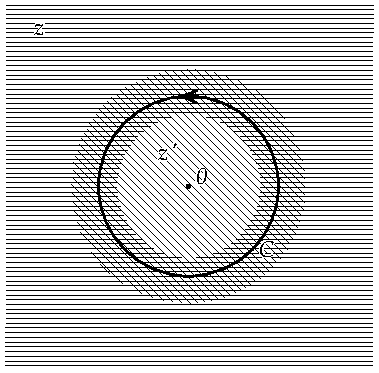
\includegraphics[width=0.8\linewidth]{figures/fig_5_3.pdf}
\caption{座標パッチ $z'$（斜線）と $z$（横線）。頂点演算子は $z'=0$ にある。環状領域では $z=z'+z_v$。}
\label{fig:5.3}
\end{figure}

隣り合うパッチの周りの輪郭積分\hyperref[eq:5.4.12]{(5.4.12)}を合わせると、
\begin{equation}
\begin{aligned}
\frac{1}{2\pi}(b,\mu_k)
=\frac{1}{2\pi i}\sum_{(mn)}\int_{C_{mn}}
\biggl[
&dz_m\,\left.\frac{\partial z_m}{\partial t^k}\right|_{z_n}
b_{z_mz_m}\\
&-d\bar z_m\,\left.\frac{\partial\bar z_m}{\partial t^k}\right|_{z_n}
b_{\bar z_m\bar z_m}
\biggr]
\end{aligned}
\tag{5.4.15}\label{eq:5.4.15}
\end{equation}
となり、これは遷移関数の微分に比例している。和は重なり合うパッチのすべての対にわたる。輪郭 $C_{mn}$ はパッチ $m$ と $n$ の間を通り、$m$ から見て反時計回りである。$(mn)$ の項は、見かけ上は明らかでないものの、$m$ と $n$ の交換について対称である。各輪郭は、閉じるか、パッチ $m,n,p$ の三重の重なりで終わる。そこで輪郭 $C_{mn}$、$C_{np}$、$C_{pm}$ は一点で交わる。これで $b$ の挿入は、Riemann面を定義するデータ、すなわち正則な同値を法とした遷移関数だけで表された。

その例として、この結果を用いれば、計量のモジュライと頂点演算子の位置のモジュライを、より対等な立場で扱える。座標系 $z$ で位置 $z_v$ にある頂点演算子を考えよう。図\ref{fig:5.3}のように、頂点演算子を中心に、小さな新しい座標パッチ $z'$ を作る。頂点演算子を座標点 $z'=0$ に保ち、その位置を、環状の重なり領域での遷移関数
\begin{equation}
z=z'+z_v
\tag{5.4.16}\label{eq:5.4.16}
\end{equation}
に組み込む。モジュライ $z_v,\bar z_v$ に対する測度は式\hyperref[eq:5.4.15]{(5.4.15)}で与えられ、ここでは
\begin{equation}
\left.\frac{\partial z'}{\partial z_v}\right|_z=-1
\tag{5.4.17}\label{eq:5.4.17}
\end{equation}
である。したがって、ゴーストの挿入は
\begin{equation}
\int_C\frac{dz'}{2\pi i}\,b_{z'z'}
\int_C\frac{d\bar z'_m}{-2\pi i}\,b_{\bar z'\bar z'}
=b_{-1}\tilde b_{-1}\mathbin{\cdot}
\tag{5.4.18}\label{eq:5.4.18}
\end{equation}
となる。$C$ は、図に示したように頂点演算子を取り囲む任意の輪郭である。そこで、S 行列の完全な式は簡潔に
\begin{equation}
S(1;\ldots;n)
=\sum_{\text{コンパクトな位相}}
e^{-\lambda\chi}\int_F\frac{d^m t}{n_R}
\left\langle\prod_{k=1}^{m}B_k
\prod_{i=1}^{n}\hat{\mathcal V}_i\right\rangle
\tag{5.4.19}\label{eq:5.4.19}
\end{equation}
と書ける。ここで $B_k$ は $b$ ゴーストの挿入\hyperref[eq:5.4.15]{(5.4.15)}の略記であり、$\hat{\mathcal V}$ は閉弦では $\tilde c c\mathcal V_{\mathrm m}$、開弦では $t_ac^a\mathcal V_{\mathrm m}$ を表す。つまり、すべての頂点演算子を固定したものとして扱い、それらの座標を遷移関数の追加のパラメータに置き換えたのである。モジュライの数 $m$ は
\begin{equation}
m=\mu+2n_{\mathrm c}+n_{\mathrm o}-\kappa
=-3\chi+2n_{\mathrm c}+n_{\mathrm o}
\tag{5.4.20}\label{eq:5.4.20}
\end{equation}
である。ここで $n_{\mathrm c}$ と $n_{\mathrm o}$ は、それぞれ閉弦と開弦の頂点演算子の数である。

式\hyperref[eq:5.4.19]{(5.4.19)}は、$\tilde c c$ または $t_ac^a$ を伴う、ハットを付した頂点演算子が基本的なものであることを示している。これは状態・演算子対応から得られるものであり、BRST 不変である。頂点演算子を積分する場合には、ゴーストの挿入\hyperref[eq:5.4.18]{(5.4.18)}が単に $\tilde c c$ または $t_ac^a$ を取り除く。たとえば、
\begin{equation}
b_{-1}\tilde b_{-1}\mathbin{\cdot}
\tilde c c\mathcal V_{\mathrm m}=\mathcal V_{\mathrm m}
\tag{5.4.21}\label{eq:5.4.21}
\end{equation}
となり、頂点演算子の積分する形式が残る。結果\hyperref[eq:5.4.19]{(5.4.19)}は Polyakov 経路積分から導いたので、頂点演算子は OCQ の形で現れたが、ここからは任意の BRST 不変な頂点演算子を用いることができる。

\subsectionlink*{演習}
\addcontentsline{toc}{subsection}{第5章の演習}

\subsubsectionlink*{演習5.1}
和\hyperref[eq:5.1.1]{(5.1.1)}を考える。ただし、今度は時空の与えられた点から始まり、与えられた点で終わる、すべての粒子の経路について和をとる。この場合、テトラッドを固定すると座標の自由度は残らない。
\begin{enumerate}
\item[(a)] ゲージ固定した経路積分\hyperref[eq:5.3.9]{(5.3.9)}に相当するものを導け。
\item[(b)] 式\hyperref[eq:5.3.18]{(5.3.18)}のように、ゴースト経路積分を行列式に帰着せよ。
\item[(c)] $X^\mu$ の経路積分を行列式に帰着せよ（弦については第6.2節でこれを行う）。
\item[(d)] 有限次元の行列式と汎関数行列式を評価し、結果が質量 $m$ の粒子のスカラー伝播関数になることを示せ。
\end{enumerate}

\subsubsectionlink*{演習5.2}
閉じたループをなす経路について、前問の各手順を繰り返せ。残留ゲージ対称性を固定するために、$m^2$ で微分することで仮の頂点演算子を導入せよ。答えは式(7.3.9)に与えられている。演習5.1と5.2の両方を解いた場合には、モジュライの測度について得られた結果どうしの関係を論じよ。

\subsubsectionlink*{演習5.3}
\begin{enumerate}
\item[(a)] $\mathcal V_{\mathrm m}$ が $(1,1)$ 物質テンソルであるとき、頂点演算子 $\tilde c c\mathcal V_{\mathrm m}$ が BRST 不変であることを、BRST カレントとの OPE から示せ。
\item[(b)] この頂点演算子が式\hyperref[eq:5.4.5]{(5.4.5)}を満たすことを示せ。
\end{enumerate}

\clearpage
% 原書166--184頁（PDF188--206）、第6章導入および6.1--6.4。
\sectionlink{ツリーレベルの振幅}\label{ch:6}

弦の相互作用を研究する準備が整った。本章では、正の Euler 数を持つ曲面から生じる最低次の振幅を考える。まず、関係する Riemann 面を記述し、必要となる CFT の期待値を計算する。次に散乱振幅を、最初は開弦について、続いて閉弦について調べる。その途中で、開弦理論の重要な一般化である Chan--Paton 因子を導入する。節の最後では CFT に戻り、期待値の一般的な性質をいくつか議論する。

\subsectionlink{Riemann 面}\label{sec:6.1}

正の Euler 数を持つ Riemann 面は、球面、円板、射影平面の三つである。

\subsubsectionlink*{球面}

球面 $S_2$ は、図\ref{fig:6.1} のように二つの座標近傍で覆うことができる。$\rho>1$ として円板 $|z|<\rho$ と $|u|<\rho$ を取り、
\begin{equation}
u=1/z
\tag{6.1.1}\label{eq:6.1.1}
\end{equation}
を満たす点を同一視して貼り合わせる。実際には $\rho\to\infty$ としてもよい。このとき座標 $z$ は「北極」$u=0$ を除くすべての場所で有効である。北極での振る舞いが正則であることを確認する場合を除けば、主に $z$ 座標近傍で計算できる。

両方の座標近傍で平坦な計量を取り、それらを共形変換（座標変換と Weyl 変換）で結ぶことにより、球面を Riemann 面と考えることができる。あるいは、大域的に定義された計量を備えた Riemann 多様体と考えてもよい。一般的な共形ゲージの計量は
\begin{equation}
ds^2=\exp(2\omega(z,\bar z))\,dz\,d\bar z
\tag{6.1.2}\label{eq:6.1.2}
\end{equation}
である。

\begin{figure}[htbp]
\centering
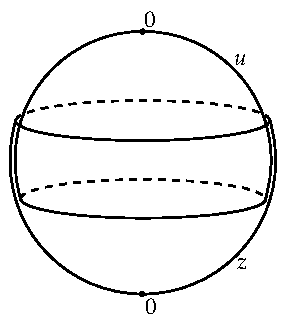
\includegraphics[width=0.65\linewidth]{figures/fig_6_1.pdf}
\caption{$z$ および $u$ 座標近傍から構成した球面。}\label{fig:6.1}
\end{figure}

$dz\,d\bar z=|z|^4du\,d\bar u$ なので、計量が $u=0$ で特異でないための条件は、$z\to\infty$ で $\exp(2\omega(z,\bar z))$ が $|z|^{-4}$ として減衰することである。たとえば、
\begin{equation}
ds^2=\frac{4r^2dz\,d\bar z}{(1+z\bar z)^2}
=\frac{4r^2du\,d\bar u}{(1+u\bar u)^2}
\tag{6.1.3}\label{eq:6.1.3}
\end{equation}
は、半径 $r$、曲率 $R=2/r^2$ の球面を表す。

第5.2節の一般的な議論によれば、球面にはモジュライがなく、六つの CKV がある。したがって特に、すべての計量は、丸い球面の計量 \hyperref[eq:6.1.3]{(6.1.3)} と $(\mathrm{diff}\times\mathrm{Weyl})$ 同値である。これを無限小のレベルで見てみよう。式 \hyperref[eq:5.2.8a]{(5.2.8)} と同様に、正則なテンソル場 $\delta g_{zz}(z)$ と正則なベクトル場 $\delta z(z)$ を探す。これらは球面全体で定義されていなければならないので、$u$ 座標近傍への変換を考える必要がある：
\begin{align}
\delta u&=\frac{\partial u}{\partial z}\delta z=-z^{-2}\delta z,
\tag{6.1.4a}\label{eq:6.1.4a}\\
\delta g_{uu}&=\left(\frac{\partial u}{\partial z}\right)^{-2}\delta g_{zz}=z^4\delta g_{zz}.
\tag{6.1.4b}\label{eq:6.1.4b}
\end{align}
正則な2次微分形式 $\delta g_{zz}$ は、$z$ に関して正則でありながら、無限遠で $z^{-4}$ として消えなければならないので、恒等的にゼロである。一方、CKV $\delta z$ は、$z\to\infty$ で $z^2$ より速く増大しなければ、$u=0$ で正則である。したがって一般的な CKV は
\begin{align}
\delta z&=a_0+a_1z+a_2z^2,
\tag{6.1.5a}\label{eq:6.1.5a}\\
\delta\bar z&=a_0^*+a_1^*\bar z+a_2^*\bar z^2,
\tag{6.1.5b}\label{eq:6.1.5b}
\end{align}
となり、Riemann--Roch の定理から予想されるように、複素パラメータ三つ、すなわち実パラメータ六つを持つ。

これらの無限小変換を指数化すると、複素数 $\alpha,\beta,\gamma,\delta$ に対する Möbius 群
\begin{equation}
z'=\frac{\alpha z+\beta}{\gamma z+\delta}
\tag{6.1.6}\label{eq:6.1.6}
\end{equation}
が得られる。$\alpha,\beta,\gamma,\delta$ を一斉に定数倍しても変換は変わらないので、$\alpha\delta-\beta\gamma=1$ と固定し、$\alpha,\beta,\gamma,\delta$ の全体の符号反転で同一視できる。これにより群 $PSL(2,\mathbb C)$ が定義される。これは $S_2$ 全体で正則な最も一般的な座標変換である。無限遠点を含めれば一対一である。六つのパラメータのうち三つは通常の回転に対応し、$PSL(2,\mathbb C)$ の $SO(3)$ 部分群をなす。

\subsubsectionlink*{円板}

反射によって点を同一視し、球面から円板 $D_2$ を構成すると便利である。たとえば、
\begin{equation}
z'=1/\bar z
\tag{6.1.7}\label{eq:6.1.7}
\end{equation}
を満たす点 $z$ と $z'$ を同一視する。極座標 $z=re^{i\phi}$ では、この変換は角度を変えずに半径を逆数にするので、単位円板 $|z|\leq1$ が同一視に対する基本領域となる。単位円周上の点は反射によって固定されるので、ここが境界になる。共形同値な反射
\begin{equation}
z'=\bar z
\tag{6.1.8}\label{eq:6.1.8}
\end{equation}
を用いた方が便利な場合も多い。この場合は上半平面が基本領域となり、実軸が境界となる。

円板の CKG は、円板の境界を固定する $PSL(2,\mathbb C)$ の部分群である。反射 \hyperref[eq:6.1.8]{(6.1.8)} では、これはちょうど \hyperref[eq:6.1.6]{(6.1.6)} で $\alpha,\beta,\gamma,\delta$ がすべて実数となる部分群であり、実パラメータの Möbius 群 $PSL(2,\mathbb R)$ である。一つの CKV は、円板の通常の回転対称性である。ここでもすべての計量は同値であり、モジュライはない。

\subsubsectionlink*{射影平面}

射影平面 $RP_2$ も、球面の $\mathbb Z_2$ 同一視として得られる。
\begin{equation}
z'=-1/\bar z
\tag{6.1.9}\label{eq:6.1.9}
\end{equation}
を満たす点 $z$ と $z'$ を同一視する。これらの点は、丸い計量 \hyperref[eq:6.1.3]{(6.1.3)} では直径の両端に位置する。不動点がないので、得られる空間に境界はないが、この空間は向き付けられていない。同一視に対する基本領域の一つは単位円板 $|z|\leq1$ であり、点 $e^{i\phi}$ と $-e^{i\phi}$ を同一視する。別の選択は $z$ 上半平面である。モジュライはない。CKG は同一視 \hyperref[eq:6.1.9]{(6.1.9)} を保つ $PSL(2,\mathbb C)$ の部分群であり、これは通常の回転群 $SO(3)$ にほかならない。

円板と射影平面はいずれも、$\mathbb Z_2$ 変換、すなわち対合で点を同一視した球面として表された。実際、すべての世界面は、向き付けられた閉じた世界面に一つまたは二つの $\mathbb Z_2$ による同一視を施して得られる。その場合、鏡像法を用いて Green 関数を求めることができる。

\subsectionlink{スカラー場の期待値}\label{sec:6.2}

必要となる基本的な量は、頂点演算子の積の期待値である。有用な技法と見方をいくつか身につけるため、三つの異なる方法でこれらを計算する。経路積分を直接評価する方法、正則性を利用する方法、そして本章の後半で用いる演算子による方法である。

経路積分による方法は、第5.3節の Faddeev--Popov 行列式と、付録の調和振動子ですでに用いた。任意の $J_\mu(\sigma)$ に対する生成汎関数
\begin{equation}
Z[J]=\left\langle\exp\left(i\int d^2\sigma\,J(\sigma)\cdot X(\sigma)\right)\right\rangle
\tag{6.2.1}\label{eq:6.2.1}
\end{equation}
から始める。今は任意のコンパクトな2次元曲面 $M$ と、任意の時空次元 $d$ を考える。$X^\mu(\sigma)$ を完全系 $\mathsf X_I(\sigma)$ で展開する：
\begin{align}
X^\mu(\sigma)&=\sum_I x_I^\mu\mathsf X_I(\sigma),
\tag{6.2.2a}\label{eq:6.2.2a}\\
\nabla^2\mathsf X_I&=-\omega_I^2\mathsf X_I,
\tag{6.2.2b}\label{eq:6.2.2b}\\
\int_M d^2\sigma\,g^{1/2}\mathsf X_I\mathsf X_{I'}&=\delta_{II'}.
\tag{6.2.2c}\label{eq:6.2.2c}
\end{align}
すると
\begin{equation}
Z[J]=\prod_{I,\mu}\int dx_I^\mu\,
\exp\left(-\frac{\omega_I^2x_I^\mu x_{I\mu}}{4\pi\alpha'}+ix_I^\mu J_{I\mu}\right),
\tag{6.2.3}\label{eq:6.2.3}
\end{equation}
ただし
\begin{equation}
J_I^\mu=\int d^2\sigma\,J^\mu(\sigma)\mathsf X_I(\sigma)
\tag{6.2.4}\label{eq:6.2.4}
\end{equation}
である。定数モード
\begin{equation}
\mathsf X_0=\left(\int d^2\sigma\,g^{1/2}\right)^{-1/2}
\tag{6.2.5}\label{eq:6.2.5}
\end{equation}
を除けば、積分は Gaussian 積分である。定数モードでは作用がゼロなので、デルタ関数を与える。積分を実行すると、
\begin{equation}
\begin{aligned}
Z[J]&=i(2\pi)^d\delta^d(J_0)\prod_{I\ne0}
\left(\frac{4\pi^2\alpha'}{\omega_I^2}\right)^{d/2}
\exp\left(-\frac{\pi\alpha'J_I\cdot J_I}{\omega_I^2}\right)\\
&=i(2\pi)^d\delta^d(J_0)
\left(\det{}'\frac{-\nabla^2}{4\pi^2\alpha'}\right)^{-d/2}\\
&\qquad\times\exp\left(-\frac12\int d^2\sigma\,d^2\sigma'\,
J(\sigma)\cdot J(\sigma')G'(\sigma,\sigma')\right).
\end{aligned}
\tag{6.2.6}\label{eq:6.2.6}
\end{equation}
第2.1節、さらに第3.2節で議論したように、時間的なモード $x_I^0$ は符号が逆の Gaussian 積分を生じ、$I\ne0$ に対する積分路の回転 $x_I^0\to-ix_I^d$ によって定義される。\footnote[1]{式 \hyperref[eq:6.2.6]{(6.2.6)} には、$S$ 行列に必要であるため、奇妙な因子 $i$ を手で挿入してある。しかし形式的には、これも同じ回転から生じると理解できる。場全体を $X^0\to-iX^d$ と回転したなら、場の再スケーリングについての通常の議論（付録の脚注1）により、Jacobian は1であるはずだ。しかし $x_0^0$ はエネルギーのデルタ関数を生むモードなので、回転させたくない。したがってこれを回転して戻す必要があり、その結果、因子 $i$ が生じる。}プライム付きの Green 関数ではゼロモードの寄与を除いている：
\begin{equation}
G'(\sigma_1,\sigma_2)=\sum_{I\ne0}\frac{2\pi\alpha'}{\omega_I^2}
\mathsf X_I(\sigma_1)\mathsf X_I(\sigma_2).
\tag{6.2.7}\label{eq:6.2.7}
\end{equation}
これは微分方程式
\begin{equation}
\begin{aligned}
-\frac1{2\pi\alpha'}\nabla^2G'(\sigma_1,\sigma_2)
&=\sum_{I\ne0}\mathsf X_I(\sigma_1)\mathsf X_I(\sigma_2)\\
&=g^{-1/2}\delta^2(\sigma_1-\sigma_2)-\mathsf X_0^2
\end{aligned}
\tag{6.2.8}\label{eq:6.2.8}
\end{equation}
を満たす。ここでは $\mathsf X_I$ の完全性を用いた。デルタ関数の源を持つ通常の Green 関数は存在しない。それは単一の電荷による静電ポテンシャルに対応するが、コンパクトな曲面では、その源から出る電気力線の行き場がないからである。$\mathsf X_0^2$ の項は、電荷を中和する背景電荷分布と考えることができる。

\subsubsectionlink*{球面}

球面に限定すると、微分方程式 \hyperref[eq:6.2.8]{(6.2.8)} の解は
\begin{equation}
G'(\sigma_1,\sigma_2)=-\frac{\alpha'}2\ln|z_{12}|^2
+f(z_1,\bar z_1)+f(z_2,\bar z_2),
\tag{6.2.9}\label{eq:6.2.9}
\end{equation}
ただし
\begin{equation}
f(z,\bar z)=\frac{\alpha'\mathsf X_0^2}4
\int d^2z'\,\exp[2\omega(z',\bar z')]\ln|z-z'|^2+k
\tag{6.2.10}\label{eq:6.2.10}
\end{equation}
である。定数 $k$ は $G'$ が $\mathsf X_0$ に直交する性質から決まるが、いずれにせよ関数 $f$ はすべての期待値から消えることが分かる。これは背景電荷から生じるが、ゼロモード積分のデルタ関数が全体の中性条件 $J_0^\mu=0$ を強制するため、背景は正味の寄与をしない。

次に、タキオンの頂点演算子の積を含む経路積分を考える：
\begin{equation}
A_{S_2}^n(k,\sigma)=\left\langle
\left[e^{ik_1\cdot X(\sigma_1)}\right]_{\mathrm r}
\left[e^{ik_2\cdot X(\sigma_2)}\right]_{\mathrm r}\cdots
\left[e^{ik_n\cdot X(\sigma_n)}\right]_{\mathrm r}
\right\rangle_{S_2}.
\tag{6.2.11}\label{eq:6.2.11}
\end{equation}
これは
\begin{equation}
J(\sigma)=\sum_{i=1}^n k_i\delta^2(\sigma-\sigma_i)
\tag{6.2.12}\label{eq:6.2.12}
\end{equation}
に対応する。このとき振幅 \hyperref[eq:6.2.6]{(6.2.6)} は
\begin{equation}
\begin{aligned}
A_{S_2}^n(k,\sigma)&=iC_{S_2}^X(2\pi)^d\delta^d\!\left(\sum_i k_i\right)\\
&\quad\times\exp\left(-\sum_{\substack{i,j=1\\i<j}}^n
k_i\cdot k_jG'(\sigma_i,\sigma_j)
-\frac12\sum_{i=1}^n k_i^2G'_{\mathrm r}(\sigma_i,\sigma_i)\right)
\end{aligned}
\tag{6.2.13}\label{eq:6.2.13}
\end{equation}
となる。ここでの定数は
\begin{equation}
C_{S_2}^X=\mathsf X_0^{-d}
\left(\det{}'\frac{-\nabla^2}{4\pi^2\alpha'}\right)_{S_2}^{-d/2}
\tag{6.2.14}\label{eq:6.2.14}
\end{equation}
である。この行列式は正則化して計算できるが、明示的に計算する必要はない。ここでは第3.6節で用いた簡単な繰り込みを採用しているので、自己縮約には
\begin{equation}
G'_{\mathrm r}(\sigma,\sigma')=G'(\sigma,\sigma')+\frac{\alpha'}2\ln d^2(\sigma,\sigma')
\tag{6.2.15}\label{eq:6.2.15}
\end{equation}
が現れる。
\begin{equation}
G'_{\mathrm r}(\sigma,\sigma)=2f(z,\bar z)+\alpha'\omega(z,\bar z)
\tag{6.2.16}\label{eq:6.2.16}
\end{equation}
は、そうなるように定義したとおり有限である。このとき球面上の経路積分は
\begin{equation}
A_{S_2}^n(k,\sigma)=iC_{S_2}^X(2\pi)^d\delta^d\!\left(\sum_i k_i\right)
\exp\left(-\frac{\alpha'}2\sum_i k_i^2\omega(\sigma_i)\right)
\prod_{\substack{i,j=1\\i<j}}^n|z_{ij}|^{\alpha'k_i\cdot k_j}.
\tag{6.2.17}\label{eq:6.2.17}
\end{equation}
関数 $f$ は、述べたとおり消えた。共形因子 $\omega(\sigma)$ への依存性は、第3.6節で頂点演算子の Weyl アノマリーから求めたものと正確に一致する。オンシェルの演算子では、これが $g^{1/2}$ の変化を打ち消す。\footnote[2]{定数 $C_{S_2}^X$ も共形因子に依存する。$X^\mu$ の CFT は、それだけではゼロでない中心電荷を持つからである。しかし完全な弦理論では、この依存性は相殺する。}すべての頂点演算子を含む大きな領域で平坦な計量を取れば（「曲率を無限遠へ押しやれば」）、$\omega(\sigma_i)$ を含む項は消える。

高いレベルの頂点演算子は、指数関数に $X^\mu$ の微分を掛けたものなので、
\begin{equation}
\left\langle\prod_{i=1}^n\left[e^{ik_i\cdot X(z_i,\bar z_i)}\right]_{\mathrm r}
\prod_{j=1}^p\partial X^{\mu_j}(z'_j)
\prod_{k=1}^q\bar\partial X^{\nu_k}(\bar z''_k)\right\rangle_{S_2}
\tag{6.2.18}\label{eq:6.2.18}
\end{equation}
も必要となる。これはすべての縮約について和を取れば得られる。その際、各 $\partial X$ または $\bar\partial X$ は、指数関数か、別の $\partial X$ または $\bar\partial X$ と縮約しなければならない。$XX$ の縮約は単に $-\tfrac12\alpha'\ln|z|^2$ であり、$f$ はここでも最終的な表式から消える。結果は
\begin{equation}
\begin{aligned}
&iC_{S_2}^X(2\pi)^d\delta^d\!\left(\sum_i k_i\right)
\prod_{\substack{i,j=1\\i<j}}^n|z_{ij}|^{\alpha'k_i\cdot k_j}\\
&\quad\times\left\langle
\prod_{j=1}^p\left[v^{\mu_j}(z'_j)+q^{\mu_j}(z'_j)\right]
\prod_{k=1}^q\left[\widetilde v^{\nu_k}(\bar z''_k)+\widetilde q^{\nu_k}(\bar z''_k)\right]
\right\rangle
\end{aligned}
\tag{6.2.19}\label{eq:6.2.19}
\end{equation}
とまとめられる。ここで
\begin{equation}
v^\mu(z)=-i\frac{\alpha'}2\sum_{i=1}^n\frac{k_i^\mu}{z-z_i},
\qquad
\widetilde v^\mu(\bar z)=-i\frac{\alpha'}2\sum_{i=1}^n\frac{k_i^\mu}{\bar z-\bar z_i}
\tag{6.2.20}\label{eq:6.2.20}
\end{equation}
は指数関数との縮約から生じる。$q^\mu=\partial X^\mu-v^\mu$ の期待値は、$-\eta^{\mu\nu}(z-z')^{-2}\alpha'/2$ を用いたすべての縮約の和で与えられ、$\widetilde q^\nu$ の期待値はその共役で与えられる。

次に、正則性を用いる別の方法で計算を繰り返す。例として
\begin{equation}
\langle\partial X^\mu(z_1)\partial X^\nu(z_2)\rangle_{S_2}
\tag{6.2.21}\label{eq:6.2.21}
\end{equation}
を考える。OPE によれば、これは
\begin{equation}
-\frac{\alpha'\eta^{\mu\nu}}{2z_{12}^2}\langle1\rangle_{S_2}+g(z_1,z_2)
\tag{6.2.22}\label{eq:6.2.22}
\end{equation}
という形を取る。$g(z_1,z_2)$ は両方の変数に関して正則である。$u$ 座標近傍では
\begin{equation}
\partial_uX^\mu=-z^2\partial_zX^\mu
\tag{6.2.23}\label{eq:6.2.23}
\end{equation}
なので、$u=0$ での正則性の条件は、$\partial_zX^\mu$ の期待値が無限遠で $z^{-2}$ として減衰することである。より一般には、共形ウェイト $(h,0)$ のテンソルは、無限遠で $z^{-2h}$ として振る舞わなければならない。$z_2$ を固定して式 \hyperref[eq:6.2.22]{(6.2.22)} の $z_1$ 依存性に着目すると、これは $g(z_1,z_2)$ が無限遠で $z_1^{-2}$ として減衰することを意味し、したがって正則性によりゼロとなる。これで、規格化を除いて期待値が決まる。経路積分の結果 \hyperref[eq:6.2.19]{(6.2.19)} と比較すると一致するが、規格化 $\langle1\rangle_{S_2}$ は $\delta(0)$ として発散することが分かる。これは、時空の無限大の体積によるゼロモードの発散にほかならない。

この方法で頂点演算子の積の期待値
\begin{equation}
A_{S_2}^n(k,\sigma)=\left\langle\prod_{i=1}^n:e^{ik_i\cdot X(z_i,\bar z_i)}:\right\rangle_{S_2}
\tag{6.2.24}\label{eq:6.2.24}
\end{equation}
を得るには、もう少し間接的な手順が必要である。指数関数は正則ではないからである。実際には正則部分と反正則部分に分解できるが、これは微妙な点を含むため、第8章で行うように演算子の言葉で導入するのがよい。ここでは並進カレントの正則性を用いる。カレント $\partial X^\mu(z)$ を一つ加えた期待値を考える。このカレントと頂点演算子との OPE により、$z$ に関する特異点が決まる：
\begin{equation}
\begin{aligned}
\left\langle\partial X^\mu(z)\prod_{i=1}^n:e^{ik_i\cdot X(z_i,\bar z_i)}:\right\rangle_{S_2}
&=-\frac{i\alpha'}2A_{S_2}^n(k,\sigma)\sum_{i=1}^n\frac{k_i^\mu}{z-z_i}\\
&\quad+\text{$z$ に関して正則な項}.
\end{aligned}
\tag{6.2.25}\label{eq:6.2.25}
\end{equation}
ここで $z\to\infty$ を見る。$\partial_uX^\mu$ が $u=0$ で正則であるという条件は、やはり $z\to\infty$ で期待値が $z^{-2}$ として消えることを要求する。したがって式 \hyperref[eq:6.2.25]{(6.2.25)} の正則な項はゼロでなければならず、$z^{-1}$ の次数の項が消えることから運動量保存
\begin{equation}
A_{S_2}^n(k,\sigma)\sum_{i=1}^n k_i^\mu=0
\tag{6.2.26}\label{eq:6.2.26}
\end{equation}
が再び得られる。

これを少し違う言い方でも述べておこう。時空並進カレントの周回積分
\begin{equation}
p^\mu=\frac1{2\pi i}\oint_C(dz\,j_z^\mu-d\bar z\,j_{\bar z}^\mu)
\tag{6.2.27}\label{eq:6.2.27}
\end{equation}
を考える。積分路 $C$ は、すべての指数関数演算子を囲んでいる。これを評価する方法は二つある。一つは、$C$ を縮めて各頂点演算子を囲む小円にする方法であり、各 OPE から $(z-z_i)^{-1}$ の項を拾って $\sum_{i=1}^n k_i^\mu$ を与える。もう一つは、$C$ を広げて $u$ 座標近傍の小円にする方法であり、$u=0$ での正則性によりゼロとなる。このような「積分路を引っ張る」議論は、CFT でよく用いられる。

OPE を用いて特異点を決め、次に正則性を用いて完全な $z$ 依存性を得た。今度は $z\to z_1$ における OPE の第2項を見る。結果 \hyperref[eq:6.2.25]{(6.2.25)} を展開すると、
\begin{equation}
-\frac{i\alpha'}2A_{S_2}^n(k,\sigma)
\left(\frac{k_1^\mu}{z-z_1}+\sum_{i=2}^n\frac{k_i^\mu}{z_1-z_i}+O(z-z_1)\right).
\tag{6.2.28}\label{eq:6.2.28}
\end{equation}
これを $ik_1^\mu$ と縮約すると、$(z-z_1)^0$ の次数の項は OPE
\begin{equation}
\begin{aligned}
ik_1\cdot\partial X(z):e^{ik_1\cdot X(z_1,\bar z_1)}:
&=\frac{\alpha'k_1^2}{2(z-z_1)}:e^{ik_1\cdot X(z_1,\bar z_1)}:\\
&\quad+\partial_{z_1}:e^{ik_1\cdot X(z_1,\bar z_1)}:+O(z-z_1)
\end{aligned}
\tag{6.2.29}\label{eq:6.2.29}
\end{equation}
と一致しなければならない。したがって
\begin{equation}
\partial_{z_1}A_{S_2}^n(k,\sigma)=\frac{\alpha'}2A_{S_2}^n(k,\sigma)
\sum_{i=2}^n\frac{k_1\cdot k_i}{z_{1i}}.
\tag{6.2.30}\label{eq:6.2.30}
\end{equation}
積分し、共役の方程式と運動量保存を用いれば、規格化を除いて経路積分が決まる：
\begin{equation}
A_{S_2}^n(k,\sigma)\propto\delta^d\!\left(\sum_i k_i\right)
\prod_{\substack{i,j=1\\i<j}}^n|z_{ij}|^{\alpha'k_i\cdot k_j}.
\tag{6.2.31}\label{eq:6.2.31}
\end{equation}
これは最初の方法と一致する。比較するには、$[\ ]_{\mathrm r}=:\ :$ となるよう、曲率を無限遠へ押しやらなければならない（$\omega(\sigma_i)=0$）ことに注意しよう。

経路積分による方法の途中の段階では、Riemann 計量の具体的な選択に細かく依存することに注目したい。これらの段階で座標不変性を保つには、計量が必要なのである。Weyl 同値でも異なる計量を選べば、Laplacian と固有関数は異なるものになる。ただし弦理論では、最後にはこの依存性が消えなければならない。第2の方法では、Riemann 面の基本的なデータである正則構造だけを用いる。

\subsubsectionlink*{円板}

円板への一般化は容易である。先ほどの球面の表示を取り、$z$ を複素平面の上半分に制限して円板を表す。Neumann 境界項は、鏡像電荷によって取り入れられる：
\begin{equation}
G'(\sigma_1,\sigma_2)=-\frac{\alpha'}2\ln|z_1-z_2|^2
-\frac{\alpha'}2\ln|z_1-\bar z_2|^2.
\tag{6.2.32}\label{eq:6.2.32}
\end{equation}
ここでは運動量保存によって消える項を省いた。すると
\begin{equation}
\begin{aligned}
\left\langle\prod_{i=1}^n:e^{ik_i\cdot X(z_i,\bar z_i)}:\right\rangle_{D_2}
&=iC_{D_2}^X(2\pi)^d\delta^d\!\left(\sum_i k_i\right)
\prod_{i=1}^n|z_i-\bar z_i|^{\alpha'k_i^2/2}\\
&\quad\times\prod_{\substack{i,j=1\\i<j}}^n
|z_i-z_j|^{\alpha'k_i\cdot k_j}|z_i-\bar z_j|^{\alpha'k_i\cdot k_j}.
\end{aligned}
\tag{6.2.33}\label{eq:6.2.33}
\end{equation}
$\partial_aX^\mu$ を含む期待値についても、Green 関数 \hyperref[eq:6.2.32]{(6.2.32)} を使い、縮約の和を取ればよい。$\partial X^\mu(z)\bar\partial X^\nu(\bar z')$（あるいは $q^\mu(z)\widetilde q^\nu(\bar z')$）の縮約はゼロでないことに注意しよう。

境界上の2点については、Green 関数 \hyperref[eq:6.2.32]{(6.2.32)} の二つの項が等しく、正規順序によって第1項を引いても、点の間隔がゼロになると Green 関数は発散する。そのため、境界演算子は、差し引く量を2倍にした\emph{境界正規順序}で定義しなければならない：
\providecommand{\bndnorm}[1]{\mathopen{{}^{\star}_{\star}}#1\mathclose{{}^{\star}_{\star}}}
\begin{equation}
\bndnorm{X^\mu(y_1)X^\nu(y_2)}=X^\mu(y_1)X^\nu(y_2)
+2\alpha'\eta^{\mu\nu}\ln|y_1-y_2|.
\tag{6.2.34}\label{eq:6.2.34}
\end{equation}
ここで $y$ は実軸上の座標を表す。組合せ論的な扱いは、他の正規順序の場合と同じである。境界正規順序を取った境界演算子の期待値は、内部の共形正規順序を取った演算子と同じよい性質、すなわち特異でないという性質を持つ。

内部と境界の両方に指数関数を含み、それぞれに適切な正規順序を取った期待値は、内部での結果 \hyperref[eq:6.2.33]{(6.2.33)} の適切な極限を取り、境界演算子については因子 $|z_i-\bar z_i|^{\alpha'k_i^2/2}$ を除けば得られる。明示的に、すべての指数関数が境界上にある場合は
\begin{equation}
\left\langle\prod_{i=1}^n\bndnorm{e^{ik_i\cdot X(y_i)}}\right\rangle_{D_2}
=iC_{D_2}^X(2\pi)^d\delta^d\!\left(\sum_i k_i\right)
\prod_{\substack{i,j=1\\i<j}}^n|y_i-y_j|^{2\alpha'k_i\cdot k_j}.
\tag{6.2.35}\label{eq:6.2.35}
\end{equation}
より一般には、
\begin{equation}
\begin{aligned}
&\left\langle\prod_{i=1}^n\bndnorm{e^{ik_i\cdot X(y_i)}}
\prod_{j=1}^p\partial_yX^{\mu_j}(y'_j)\right\rangle_{D_2}
=iC_{D_2}^X(2\pi)^d\delta^d\!\left(\sum_i k_i\right)\\
&\qquad\times\prod_{\substack{i,j=1\\i<j}}^n|y_{ij}|^{2\alpha'k_i\cdot k_j}
\left\langle\prod_{j=1}^p\left[v^{\mu_j}(y'_j)+q^{\mu_j}(y'_j)\right]\right\rangle_{D_2},
\end{aligned}
\tag{6.2.36}\label{eq:6.2.36}
\end{equation}
ただし今度は
\begin{equation}
v^\mu(y)=-2i\alpha'\sum_{i=1}^n\frac{k_i^\mu}{y-y_i}
\tag{6.2.37}\label{eq:6.2.37}
\end{equation}
であり、$q$ は $-2\alpha'(y-y')^{-2}\eta^{\mu\nu}$ を用いて縮約する。

\subsubsectionlink*{射影平面}

鏡像法により Green 関数は
\begin{equation}
G'(\sigma_1,\sigma_2)=-\frac{\alpha'}2\ln|z_1-z_2|^2
-\frac{\alpha'}2\ln|1+z_1\bar z_2|^2
\tag{6.2.38}\label{eq:6.2.38}
\end{equation}
と与えられる。このとき
\begin{equation}
\begin{aligned}
\left\langle\prod_{i=1}^n:e^{ik_i\cdot X(z_i,\bar z_i)}:\right\rangle_{RP_2}
&=iC_{RP_2}^X(2\pi)^d\delta^d\!\left(\sum_i k_i\right)
\prod_{i=1}^n|1+z_i\bar z_i|^{\alpha'k_i^2/2}\\
&\quad\times\prod_{\substack{i,j=1\\i<j}}^n
|z_i-z_j|^{\alpha'k_i\cdot k_j}|1+z_i\bar z_j|^{\alpha'k_i\cdot k_j}
\end{aligned}
\tag{6.2.39}\label{eq:6.2.39}
\end{equation}
となり、より一般の期待値についても同様である。この対合には不動点がないため、境界はない。点 $z$ がその鏡像 $-\bar z^{-1}$ に近づくことはできない。

\subsectionlink{\texorpdfstring{$bc$}{bc} CFT}\label{sec:6.3}

\subsubsectionlink*{球面}

ゴーストの経路積分は、第5.3節ですでに設定した。Riemann--Roch の定理によれば、ゼロでない最も簡単な期待値は
\begin{equation}
\langle c(z_1)c(z_2)c(z_3)\widetilde c(\bar z_4)\widetilde c(\bar z_5)\widetilde c(\bar z_6)\rangle_{S_2}
\tag{6.3.1}\label{eq:6.3.1}
\end{equation}
である。規格化（汎関数行列式）を除けば、結果 \hyperref[eq:5.3.18]{(5.3.18)} はゼロモードの行列式
\begin{equation}
\det\mathsf C_{0j}^{a}(\sigma_i)
\tag{6.3.2}\label{eq:6.3.2}
\end{equation}
そのものであった。六つの CKV は第6.1節で求めた。複素基底では
\begin{align}
\mathsf C^z&=1,z,z^2,\qquad \mathsf C^{\bar z}=0,
\tag{6.3.3a}\label{eq:6.3.3a}\\
\mathsf C^z&=0,\qquad \mathsf C^{\bar z}=1,\bar z,\bar z^2.
\tag{6.3.3b}\label{eq:6.3.3b}
\end{align}
この基底では行列式が二つの $3\times3$ ブロックに分かれ、期待値は
\begin{equation}
C_{S_2}^{\mathrm g}\det\begin{vmatrix}
1&1&1\\z_1&z_2&z_3\\z_1^2&z_2^2&z_3^2
\end{vmatrix}
\det\begin{vmatrix}
1&1&1\\\bar z_4&\bar z_5&\bar z_6\\\bar z_4^2&\bar z_5^2&\bar z_6^2
\end{vmatrix}
=C_{S_2}^{\mathrm g}z_{12}z_{13}z_{23}\bar z_{45}\bar z_{46}\bar z_{56}
\tag{6.3.4}\label{eq:6.3.4}
\end{equation}
となる。定数 $C_{S_2}^{\mathrm g}$ には、汎関数行列式に加えて、基底 \hyperref[eq:6.3.3a]{(6.3.3)} が正規直交していないことから生じる有限次元の Jacobian（位置には依存しない）も含まれる。

ツリーレベルの振幅で実際に必要となる $bc$ 経路積分はこれだけだが、完全を期すため、
\begin{equation}
\begin{aligned}
&\left\langle\prod_{i=1}^{p+3}c(z_i)\prod_{j=1}^p b(z'_j)\cdot(\text{反正則部分})\right\rangle_{S_2}\\
&\quad=C_{S_2}^{\mathrm g}\frac{z_{p+1,p+2}z_{p+1,p+3}z_{p+2,p+3}}
{(z_1-z'_1)\cdots(z_p-z'_p)}\cdot(\text{反正則部分})
\ \pm\ \text{置換項}
\end{aligned}
\tag{6.3.5}\label{eq:6.3.5}
\end{equation}
も示しておく。これは $b$ を $c$ と縮約して得られる。反正則部分は同じ形を持つ。ここでは全体の符号をあまり厳密に扱っていないが、やはり Faddeev--Popov 行列式については、いずれにせよ絶対値を取る。

正則性を用いる別の導出を与えるため、まず再び保存則を考える。振幅 \hyperref[eq:6.3.5]{(6.3.5)} にゴースト数の周回積分 $\oint_C dz\,j(z)/(2\pi i)$ を挿入して導く。$C$ はすべての頂点演算子を囲み、$j=-:bc:$ はこれまでと同じゴースト数カレントである。$b$ および $c$ との OPE により、これは単に $c$ の個数から $b$ の個数を引いたものを数え、元の振幅の $n_c-n_b$ 倍を与える。共形変換 \hyperref[eq:2.5.17]{(2.5.17)} を用いて、積分路を $u$ 座標近傍へ引っ張ると、
\begin{equation}
\oint_C\frac{dz}{2\pi i}j_z=-\oint_C\frac{du}{2\pi i}j_u+3\ \longrightarrow\ 3.
\tag{6.3.6}\label{eq:6.3.6}
\end{equation}
$+3$ のシフトが生じるのは、$j$ がテンソルではなく、$T$ との OPE に $z^{-3}$ の項を持つからである。最後の段階では $u$ 座標近傍での正則性を用いた。したがって、ゼロでない振幅は $n_c-n_b=3$、同様に $n_{\widetilde c}-n_{\widetilde b}=3$ を満たし、Riemann--Roch の定理と一致する。

OPE によれば、ゴーストの期待値 \hyperref[eq:6.3.1]{(6.3.1)} は各変数に関して正則であり、同一の反交換する場二つが近づくとゼロにならなければならない。したがって、位置の正則関数 $F$ と反正則関数 $\widetilde F$ を用いて
\begin{equation}
z_{12}z_{13}z_{23}\bar z_{45}\bar z_{46}\bar z_{56}
F(z_1,z_2,z_3)\widetilde F(\bar z_4,\bar z_5,\bar z_6)
\tag{6.3.7}\label{eq:6.3.7}
\end{equation}
という形でなければならない。$z_1\to\infty$ では、これは $z_1^2F$ として振る舞う。しかし $c$ は共形ウェイト $-1$ のテンソルなので、振幅は無限遠で $z_1^2$ より大きくなることはできない。したがって $F(z_i)$ は $z_1$ に依存してはならず、同様に $z_2$ と $z_3$ にも依存してはならない。$\widetilde F$ にも同じ議論を適用すると、再び結果 \hyperref[eq:6.3.4]{(6.3.4)} が得られる。同じ議論により、一般の場合 \hyperref[eq:6.3.5]{(6.3.5)} については
\begin{equation}
C_{S_2}^{\mathrm g}\prod_{\substack{i,i'=1\\i<i'}}^{p+3}z_{ii'}
\prod_{\substack{j,j'=1\\j<j'}}^p z'_{jj'}
\prod_{i=1}^{p+3}\prod_{j=1}^p(z_i-z'_j)^{-1}\cdot(\text{反正則部分})
\tag{6.3.8}\label{eq:6.3.8}
\end{equation}
が得られる。これは正しい極、零点、無限遠での振る舞いを持つ。明らかに、\hyperref[eq:6.3.5]{(6.3.5)} の置換についての和は、この一つの項にまとまる。

ここではボース弦のゴーストに関係する $\lambda=2$ の理論を考えたが、どちらの方法も任意の $\lambda$ に容易に一般化できる。

\subsubsectionlink*{円板}

円板上の $bc$ 振幅を得る最も簡単な方法は、二重化の手法である。式 \hyperref[eq:2.7.30]{(2.7.30)} と同様に、
\begin{equation}
\widetilde b(\bar z)=b(z'),\qquad \widetilde c(\bar z)=c(z'),
\qquad z'=\bar z,\quad\operatorname{Im}z>0
\tag{6.3.9}\label{eq:6.3.9}
\end{equation}
を用いれば、上半平面の正則場と反正則場の両方を、平面全体の正則場で表すことができる。正則場の期待値は球面の場合と同様に求まり、すべての $z$ に対して
\begin{equation}
\langle c(z_1)c(z_2)c(z_3)\rangle_{D_2}=C_{D_2}^{\mathrm g}z_{12}z_{13}z_{23}.
\tag{6.3.10}\label{eq:6.3.10}
\end{equation}
すると、たとえば
\begin{equation}
\begin{aligned}
\langle c(z_1)c(z_2)\widetilde c(\bar z_3)\rangle_{D_2}
&=\langle c(z_1)c(z_2)c(z'_3)\rangle_{D_2}\\
&=C_{D_2}^{\mathrm g}z_{12}(z_1-\bar z_3)(z_2-\bar z_3).
\end{aligned}
\tag{6.3.11}\label{eq:6.3.11}
\end{equation}
より一般の相関関数も同じ方法で得られる。

\subsubsectionlink*{射影平面}

ここでも二重化の手法を用いることができる。対合 $z'=-\bar z^{-1}$ から
\begin{equation}
\begin{aligned}
\widetilde b(\bar z)&=\left(\frac{\partial z'}{\partial\bar z}\right)^2b(z')=z'^4b(z'),\\
\widetilde c(\bar z)&=\left(\frac{\partial z'}{\partial\bar z}\right)^{-1}c(z')=z'^{-2}c(z')
\end{aligned}
\tag{6.3.12}\label{eq:6.3.12}
\end{equation}
が従う。やはり
\begin{equation}
\langle c(z_1)c(z_2)c(z_3)\rangle_{RP_2}=C_{RP_2}^{\mathrm g}z_{12}z_{13}z_{23}
\tag{6.3.13}\label{eq:6.3.13}
\end{equation}
なので、
\begin{equation}
\begin{aligned}
\langle c(z_1)c(z_2)\widetilde c(\bar z_3)\rangle_{RP_2}
&=z_3'^{-2}\langle c(z_1)c(z_2)c(z'_3)\rangle_{RP_2}\\
&=C_{RP_2}^{\mathrm g}z_{12}(1+z_1\bar z_3)(1+z_2\bar z_3).
\end{aligned}
\tag{6.3.14}\label{eq:6.3.14}
\end{equation}

\subsectionlink{Veneziano 振幅}\label{sec:6.4}

開弦の振幅は閉弦の振幅より少し簡単なので、まず開弦から始める。

円板を上半平面で表すと、境界座標 $y$ は実数である。モジュライはない。計量を固定した後、CKG $PSL(2,\mathbb R)$ を用いて、三つの頂点演算子を境界上の任意の位置 $y_1,y_2,y_3$ に固定できる。ただし、この群は頂点演算子の巡回順序を変えないので、二つの順序について和を取らなければならない。したがって、円板上の三つの開弦タキオンに対して、弦の $S$ 行列の一般式 \hyperref[eq:5.3.9]{(5.3.9)} は
\begin{equation}
\begin{aligned}
S_{D_2}(k_1;k_2;k_3)&=g_{\mathrm o}^3e^{-\lambda}
\left\langle\bndnorm{c^1e^{ik_1\cdot X}(y_1)}
\bndnorm{c^1e^{ik_2\cdot X}(y_2)}
\bndnorm{c^1e^{ik_3\cdot X}(y_3)}\right\rangle_{D_2}\\
&\quad+(k_2\leftrightarrow k_3)
\end{aligned}
\tag{6.4.1}\label{eq:6.4.1}
\end{equation}
に帰着し、固定した各座標の積分は対応する $c$ ゴーストで置き換わる。各頂点演算子には、開弦結合定数 $g_{\mathrm o}$ の因子を含めてある。因子 $e^{-\lambda}$ は、作用の Euler 数の項から生じる。もちろん $g_{\mathrm o}$ と $e^\lambda$ は $g_{\mathrm o}^2\propto e^\lambda$ と関係しているが、その比例定数は以下で決めていく。

\hyperref[eq:6.4.1]{(6.4.1)} の期待値は前の各節で求めた（ここでもゴーストについては絶対値を取る）。その結果、
\begin{equation}
\begin{aligned}
S_{D_2}(k_1;k_2;k_3)&=ig_{\mathrm o}^3C_{D_2}(2\pi)^{26}\delta^{26}\!\left(\sum_i k_i\right)\\
&\quad\times|y_{12}|^{1+2\alpha'k_1\cdot k_2}
|y_{13}|^{1+2\alpha'k_1\cdot k_3}|y_{23}|^{1+2\alpha'k_2\cdot k_3}
+(k_2\leftrightarrow k_3),
\end{aligned}
\tag{6.4.2}\label{eq:6.4.2}
\end{equation}
ただし $C_{D_2}=e^{-\lambda}C_{D_2}^XC_{D_2}^{\mathrm g}$ である。運動量保存と質量殻条件 $k_i^2=1/\alpha'$ により
\begin{equation}
2\alpha'k_1\cdot k_2=\alpha'(k_3^2-k_1^2-k_2^2)=-1
\tag{6.4.3}\label{eq:6.4.3}
\end{equation}
となり、他の $k_i\cdot k_j$ についても同様なので、これは
\begin{equation}
S_{D_2}(k_1;k_2;k_3)=2ig_{\mathrm o}^3C_{D_2}(2\pi)^{26}\delta^{26}\!\left(\sum_i k_i\right)
\tag{6.4.4}\label{eq:6.4.4}
\end{equation}
に帰着する。この結果はゲージの選択 $y_i$ に依存しない。これはもちろん Faddeev--Popov の手続きの一般的な性質である。ここでは Weyl 不変性が決定的に重要であり、頂点演算子を質量殻から外せば、振幅は $y_i$ の選び方に依存する。

$y_i$ に依存しないことを使えば、計算せずに Faddeev--Popov 行列式を決めることもできた。質量殻条件と運動量保存を用いると、$X^\mu$ の期待値は $|y_{12}y_{13}y_{23}|^{-1}$ に比例するので、測度はその逆数でなければならない。いずれの場合も三つの位置を固定するので、同じ測度が $n>3$ 個の頂点演算子にも適用される。

4タキオン振幅も同様に得られる：
\begin{equation}
\begin{aligned}
&S_{D_2}(k_1;k_2;k_3;k_4)\\
&=g_{\mathrm o}^4e^{-\lambda}\int_{-\infty}^{\infty}dy_4
\left\langle\prod_{i=1}^3\bndnorm{c^1(y_i)e^{ik_i\cdot X(y_i)}}
\bndnorm{e^{ik_4\cdot X(y_4)}}\right\rangle+(k_2\leftrightarrow k_3)\\
&=ig_{\mathrm o}^4C_{D_2}(2\pi)^{26}\delta^{26}\!\left(\sum_i k_i\right)
|y_{12}y_{13}y_{23}|\int_{-\infty}^{\infty}dy_4\prod_{i<j}|y_{ij}|^{2\alpha'k_i\cdot k_j}
+(k_2\leftrightarrow k_3).
\end{aligned}
\tag{6.4.5}\label{eq:6.4.5}
\end{equation}

\begin{figure}[htbp]
\centering
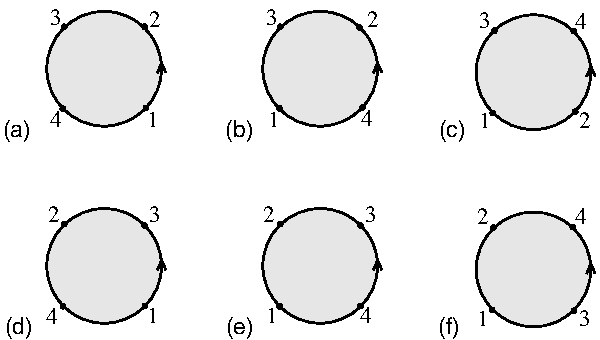
\includegraphics[width=0.9\linewidth]{figures/fig_6_2.pdf}
\caption{円板上の四つの開弦頂点演算子の、巡回的に非同値な六つの順序。座標 $y$ は矢印の向きに増加する。ただし点3では $+\infty$ から $-\infty$ へ飛ぶ。}\label{fig:6.2}
\end{figure}

これも、$y_4$ の変数変換（Möbius 変換）を行えば、$y_{1,2,3}$ に依存しない。$y_1=0$、$y_2=1$、$y_3\to\infty$ と取ると便利である。振幅は通常、Mandelstam 変数
\begin{equation}
s=-(k_1+k_2)^2,\qquad t=-(k_1+k_3)^2,\qquad u=-(k_1+k_4)^2
\tag{6.4.6}\label{eq:6.4.6}
\end{equation}
で書かれる。これらは独立ではない。運動量保存と質量殻条件から
\begin{equation}
s+t+u=\sum_i m_i^2=-\frac4{\alpha'}
\tag{6.4.7}\label{eq:6.4.7}
\end{equation}
が従う。$2\alpha'k_i\cdot k_j=-2+\alpha'(k_i+k_j)^2$ を用いると、振幅は
\begin{equation}
\begin{aligned}
S_{D_2}(k_1;k_2;k_3;k_4)&=ig_{\mathrm o}^4C_{D_2}(2\pi)^{26}\delta^{26}\!\left(\sum_i k_i\right)\\
&\quad\times\left[\int_{-\infty}^{\infty}dy_4\,|y_4|^{-\alpha'u-2}|1-y_4|^{-\alpha't-2}+(t\to s)\right]
\end{aligned}
\tag{6.4.8}\label{eq:6.4.8}
\end{equation}
となる。

積分は、$-\infty<y_4<0$、$0<y_4<1$、$1<y_4<\infty$ の三つの領域に分かれる。これら三つの領域では、頂点演算子はそれぞれ図\ref{fig:6.2}(a)、(b)、(c) のように並ぶ。Möbius 不変性を用いれば、これらの領域のどれでも他の領域へ写せるので、それらの寄与は頂点演算子の入れ替えを除いて等しい。$(t\leftrightarrow s)$ の項が図\ref{fig:6.2}(d)、(e)、(f) を与える。全部を合わせると、
\begin{equation}
\begin{aligned}
S_{D_2}(k_1;k_2;k_3;k_4)&=2ig_{\mathrm o}^4C_{D_2}(2\pi)^{26}\delta^{26}\!\left(\sum_i k_i\right)\\
&\quad\times\bigl[I(s,t)+I(t,u)+I(u,s)\bigr],
\end{aligned}
\tag{6.4.9}\label{eq:6.4.9}
\end{equation}
ただし
\begin{equation}
I(s,t)=\int_0^1dy\,y^{-\alpha's-2}(1-y)^{-\alpha't-2}.
\tag{6.4.10}\label{eq:6.4.10}
\end{equation}
三つの項は、それぞれ図\ref{fig:6.2}(c)、(f)、図\ref{fig:6.2}(b)、(d)、そして図\ref{fig:6.2}(a)、(e) から生じる。

\begin{figure}[htbp]
\centering
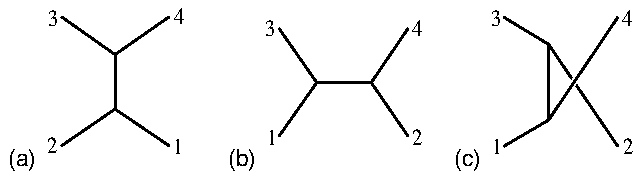
\includegraphics[width=0.9\linewidth]{figures/fig_6_3.pdf}
\caption{(a) $s$、(b) $t$、(c) $u$ チャネルの極を生じる過程。}\label{fig:6.3}
\end{figure}

積分 $I(s,t)$ は $\alpha's<-1$ かつ $\alpha't<-1$ なら収束する。$\alpha's\to-1$ では、積分は $y=0$ で発散する。この発散を調べるため、$y=0$ の近傍を取り、被積分関数を近似する：
\begin{equation}
\begin{aligned}
I(s,t)&=\int_0^rdy\,y^{-\alpha's-2}
+\text{$\alpha's=-1$ で解析的な項}\\
&=-\frac{r^{-\alpha's-1}}{\alpha's+1}
+\text{$\alpha's=-1$ で解析的な項}\\
&=-\frac1{\alpha's+1}
+\text{$\alpha's=-1$ で解析的な項}.
\end{aligned}
\tag{6.4.11}\label{eq:6.4.11}
\end{equation}
\hyperref[eq:6.4.11]{(6.4.11)} では、収束する領域で積分を評価した。この発散は、開弦タキオンの質量の二乗 $s=-1/\alpha'$ における極であることが分かる。変数 $s$ は散乱 $1+2\to3+4$ における重心系エネルギーの二乗そのものなので、この極は中間タキオン状態による共鳴である。ここでも、最も軽い弦の状態がタキオンであることはボース弦に特有であり、議論の本質には関係しない。この極は図\ref{fig:6.3}(a) に示した過程による。タキオン1と2が結合して一つのタキオンになり、これがタキオン3と4に分裂する。

$\alpha's=-1$ の特異点は単なる極なので、$I(s,t)$ はこの点を越えて $\alpha's>-1$ の領域へ解析接続できる。振幅は、この解析接続によって定義される。極における振幅の発散は、振幅の本質的な物理的特徴であり、中間の弦状態が時空の長距離を伝播することに対応する共鳴である。一方、極を越えたところで積分が発散することは、そうではない。それは振幅のこの特定の積分表示に由来するだけである。接続に問題はない。実際、弦の発散はすべて、この同じ基本的な形を持つことが分かるので、この一種類の解析接続によって、もちろん極そのものを除くすべての発散が取り除かれる。極は実軸上にあるため、さらに正確に定義する必要がある。Minkowski 過程に対する正しい $\epsilon$ 処方は
\begin{equation}
\begin{aligned}
\frac1{\alpha's+1}&\equiv\frac1{\alpha's+1+i\epsilon}\\
&\equiv\mathrm P\frac1{\alpha's+1}-i\pi\delta(\alpha's+1),
\end{aligned}
\tag{6.4.12}\label{eq:6.4.12}
\end{equation}
であり、$\mathrm P$ は主値を表す。ユニタリー性（第9章でより体系的に展開する）は、この極が存在することを要求し、その係数を、二つのタキオンが一つへ散乱する振幅によって決める：
\begin{equation}
\begin{aligned}
S_{D_2}(k_1;k_2;k_3;k_4)
&=i\int\frac{d^{26}k}{(2\pi)^{26}}
\frac{S_{D_2}(k_1;k_2;k)S_{D_2}(-k;k_3;k_4)}{-k^2+\alpha'^{-1}+i\epsilon}\\
&\quad+\text{$k^2=1/\alpha'$ で解析的な項}.
\end{aligned}
\tag{6.4.13}\label{eq:6.4.13}
\end{equation}

$I(u,s)$ からの等しい極への寄与も含めて、4タキオン振幅の因子をまとめ、3タキオンの結果 \hyperref[eq:6.4.4]{(6.4.4)} を用いると、条件 \hyperref[eq:6.4.13]{(6.4.13)} は
\begin{equation}
C_{D_2}=e^{-\lambda}C_{D_2}^XC_{D_2}^{\mathrm g}
=\frac1{\alpha'g_{\mathrm o}^2}
\tag{6.4.14}\label{eq:6.4.14}
\end{equation}
を与える。このとき3タキオン振幅は
\begin{equation}
S_{D_2}(k_1;k_2;k_3)=\frac{2ig_{\mathrm o}}{\alpha'}(2\pi)^{26}\delta^{26}\!\left(\sum_i k_i\right).
\tag{6.4.15}\label{eq:6.4.15}
\end{equation}
さまざまな汎関数行列式は消えた。ユニタリー性を用いれば、すべての規格化を、頂点演算子に現れる定数 $g_{\mathrm o}$ で表せる。実際には、行列式は注意深い正則化と繰り込みによって計算でき、異なるトポロジー間の相対的な規格化は、ユニタリー性から求めたものと一致する。

極を越えて接続すると、さらに特異点に出会う。被積分関数を $y=0$ で Taylor 展開すると、
\begin{equation}
I(s,t)=\int_0^rdy\,\left[y^{-\alpha's-2}+(\alpha't+2)y^{-\alpha's-1}+\cdots\right].
\tag{6.4.16}\label{eq:6.4.16}
\end{equation}
第2項は $\alpha's=0$ に極を与える：
\begin{equation}
I(s,t)=\frac{u-t}{2s}+\text{$\alpha's=0$ で解析的な項}.
\tag{6.4.17}\label{eq:6.4.17}
\end{equation}
Taylor 展開のさらに先の項から、振幅は
\begin{equation}
\alpha's=-1,0,1,2,\ldots
\tag{6.4.18}\label{eq:6.4.18}
\end{equation}
に極を持つ。これらは開弦の状態の位置と正確に一致する。積分 $I(s,t)$ は、変数 $t$ についても同じ位置 \hyperref[eq:6.4.18]{(6.4.18)} に極を持ち、これは端点 $y=1$ から生じる。これらは図\ref{fig:6.3}(b) の過程による。振幅 \hyperref[eq:6.4.9]{(6.4.9)} の残りの二つの項は、$s$ および $t$ チャネルの極にさらに寄与し、また図\ref{fig:6.3}(c) の $u$ チャネルの極も与える。\hyperref[eq:6.4.17]{(6.4.17)} の $s=0$ における留数は $u-t$ の奇関数なので、この極は実際には $I(s,u)$ からの極と相殺し、$1/\alpha'$ の偶数倍にあるすべての極も同様に相殺する。次節で導入する、より一般的な開弦理論では、こうはならない。

Euler のベータ関数を
\begin{equation}
B(a,b)=\int_0^1dy\,y^{a-1}(1-y)^{b-1}
\tag{6.4.19}\label{eq:6.4.19}
\end{equation}
と定義すると、
\begin{equation}
I(s,t)=B(-\alpha_{\mathrm o}(s),-\alpha_{\mathrm o}(t)),
\qquad \alpha_{\mathrm o}(x)=1+\alpha'x.
\tag{6.4.20}\label{eq:6.4.20}
\end{equation}
これはガンマ関数で表すことができる。$w$ を固定し、$y=v/w$ と置くと、
\begin{equation}
w^{a+b-1}B(a,b)=\int_0^w dv\,v^{a-1}(w-v)^{b-1}.
\tag{6.4.21}\label{eq:6.4.21}
\end{equation}
両辺に $e^{-w}$ を掛け、$\int_0^\infty dw$ で積分し、まとめ直すと、
\begin{equation}
\begin{aligned}
\Gamma(a+b)B(a,b)&=\int_0^\infty dv\,v^{a-1}e^{-v}
\int_0^\infty d(w-v)\,(w-v)^{b-1}e^{-(w-v)}\\
&=\Gamma(a)\Gamma(b).
\end{aligned}
\tag{6.4.22}\label{eq:6.4.22}
\end{equation}
したがって4タキオン振幅は
\begin{equation}
\begin{aligned}
&S_{D_2}(k_1;k_2;k_3;k_4)=\frac{2ig_{\mathrm o}^2}{\alpha'}(2\pi)^{26}\delta^{26}\!\left(\sum_i k_i\right)\\
&\quad\times\bigl[B(-\alpha_{\mathrm o}(s),-\alpha_{\mathrm o}(t))
+B(-\alpha_{\mathrm o}(s),-\alpha_{\mathrm o}(u))
+B(-\alpha_{\mathrm o}(t),-\alpha_{\mathrm o}(u))\bigr],
\end{aligned}
\tag{6.4.23}\label{eq:6.4.23}
\end{equation}
ただし
\begin{equation}
B(-\alpha_{\mathrm o}(x),-\alpha_{\mathrm o}(y))
=\frac{\Gamma(-\alpha'x-1)\Gamma(-\alpha'y-1)}{\Gamma(-\alpha'x-\alpha'y-2)}.
\tag{6.4.24}\label{eq:6.4.24}
\end{equation}
これが \emph{Veneziano 振幅}であり、もともとは強い相互作用の現象論的な特徴の一部を模型化するために書かれた。

Veneziano 振幅の高エネルギーでの振る舞いは重要である。注目すべき領域は二つあり、Regge 極限
\begin{equation}
s\to\infty,\qquad t\ \text{を固定}
\tag{6.4.25}\label{eq:6.4.25}
\end{equation}
と、硬散乱極限
\begin{equation}
s\to\infty,\qquad t/s\ \text{を固定}
\tag{6.4.26}\label{eq:6.4.26}
\end{equation}
である。散乱過程 $1+2\to3+4$ を考えると（したがって $k_1^0$ と $k_2^0$ は正であり、$k_3^0$ と $k_4^0$ は負である）、1と2の重心系では
\begin{equation}
s=E^2,\qquad t=(4m^2-E^2)\sin^2\frac\theta2,
\qquad u=(4m^2-E^2)\cos^2\frac\theta2,
\tag{6.4.27}\label{eq:6.4.27}
\end{equation}
となる。$E$ は重心系エネルギー、$\theta$ は粒子1と粒子3の間の角度である。Regge 極限は高エネルギー・小角の極限であり、硬散乱極限は高エネルギー・固定角の極限である。Stirling の近似 $\Gamma(x+1)\approx x^xe^{-x}(2\pi x)^{1/2}$ を用いると、Regge 領域での振る舞いは
\begin{equation}
S_{D_2}(k_1;k_2;k_3;k_4)\propto s^{\alpha_{\mathrm o}(t)}\Gamma(-\alpha_{\mathrm o}(t)),
\tag{6.4.28}\label{eq:6.4.28}
\end{equation}
となり、ここでも $\alpha_{\mathrm o}(t)=\alpha't+1$ である。すなわち、振幅は $s$ のべきとして変化し、そのべきは $t$ に依存する。これが Regge の振る舞いである。ガンマ関数の極では、振幅は $s$ の整数べきであり、整数スピン $\alpha_{\mathrm o}(t)$ を持つ弦の交換に対応する。

硬散乱極限では、
\begin{equation}
\begin{aligned}
S_{D_2}(k_1;k_2;k_3;k_4)
&\approx\exp\left[-\alpha'(s\ln s\alpha'+t\ln t\alpha'+u\ln u\alpha')\right]\\
&=\exp[-\alpha'sf(\theta)],
\end{aligned}
\tag{6.4.29}\label{eq:6.4.29}
\end{equation}
ただし
\begin{equation}
f(\theta)\approx-\sin^2\frac\theta2\ln\sin^2\frac\theta2
-\cos^2\frac\theta2\ln\cos^2\frac\theta2
\tag{6.4.30}\label{eq:6.4.30}
\end{equation}
は正である。結果 \hyperref[eq:6.4.29]{(6.4.29)} は注目に値する。高エネルギー・固定角の散乱は、散乱される物体の内部構造を探る。Rutherford は、アルファ粒子と原子の硬散乱によって原子核を発見した。SLAC における電子と核子の硬散乱は、核子を構成するクォークを明らかにした。場の量子論では、硬散乱振幅は $s$ のべきとして減衰する。核子のような複合物体でも、その構成要素が点状なら、振幅はべき則に従う。指数関数的な減衰 \hyperref[eq:6.4.29]{(6.4.29)} は、それよりはるかに軟らかい。結果 \hyperref[eq:6.4.29]{(6.4.29)} は、予想されるように、大きさ $\alpha'^{1/2}$ の滑らかな物体を示唆する。

ここでは0粒子、1粒子、2粒子の振幅を飛ばして、3粒子振幅から始めた。これらの振幅とその解釈は、第6.6節で議論する。


% 原文PDF206の6.5見出しからPDF227末まで。
\subsectionlink{Chan--Paton因子とゲージ相互作用}\label{sec:6.5}

本節では、開弦の質量のないベクトル状態の相互作用を考える。議論を少し興味深いものにするため、まず開弦理論の一般化を導入する。

第3章末では、非常に広いクラスのボソン弦理論を導入したが、相互作用を初めて調べるここでは、最も単純な平坦な26次元の場合に注目する。これは対称性の観点から考えられる。この理論は最大の26次元 Poincaré 不変性をもつ。閉ボソン弦では、この対称性をもつ理論はこれだけである。証明の概略は次のとおりである。時空の並進に対する世界面の Noether カレントは、ウェイト $(1,0)$ と $(0,1)$ の成分をもつ。第2.9節の議論によれば、これらのカレントは $z$ または $\bar z$ に関して正則となる。本章の計算で見たように、これだけで、すべての期待値を決定するのに十分である。

\begin{figure}[tbp]
\centering
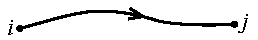
\includegraphics[width=0.52\linewidth]{figures/fig_6_4.pdf}
\caption{Chan--Paton 自由度をもつ開弦。}
\label{fig:6.4}
\end{figure}

しかし開弦理論には一般化がある。開弦は境界、すなわち端点をもつ。特別な点をもつ量子系では、内部を伝播する場に加えて、その点に存在する自由度を設けるのが自然である。開弦の各端に、$n$ 個の状態のいずれかをとりうる、Chan--Paton 自由度と呼ばれる新しい自由度を加えよう。すると弦状態の基底は
\begin{equation}
|N;k;ij\rangle
\tag{6.5.1}\label{eq:6.5.1}
\end{equation}
となる。ここで $i,j$ は左端と右端の状態を表し、1から $n$ までの値をとる。エネルギー運動量テンソルは以前と同じものと定義し、新しい自由度には依存させない。したがって、共形不変性は自動的に成り立つ。Chan--Paton 自由度は不変なので、Poincaré 不変性も自動的に成り立つ。これらの新しい自由度の世界面上の力学は自明だが、時空の物理には大きな影響を及ぼす。

強い相互作用の弦理論では、これを導入する動機は $SU(3)$ のフレーバー量子数を導入することにあった。端点は、カラー電気束管で結ばれたクォークと反クォークのようなものである。ここでは、与えられた対称性をもつすべての可能性を考えるという一般的な枠組みから動機付けている。第8章では Chan--Paton 自由度に新しい解釈を与え、第14章ではさらに解釈を精密化する可能性を述べる。

今や $n^2$ 個のスカラータキオン、$n^2$ 個の質量のないベクトルボソンなどがある。
\begin{equation}
\operatorname{Tr}(\lambda^a\lambda^b)=\delta^{ab}
\tag{6.5.2}\label{eq:6.5.2}
\end{equation}
と規格化した $n^2$ 個の Hermite 行列 $\lambda^a_{ij}$ は、二つの端点の状態の完全系である。これらは $U(n)$ の表現行列なので、質量のないベクトルは $U(n)$ ゲージ対称性に対応すると推測できる。間もなく、実際にそうであることが分かる。

基底を
\begin{equation}
|N;k;a\rangle=\sum_{i,j=1}^{n}|N;k;ij\rangle\lambda^a_{ij}
\tag{6.5.3}\label{eq:6.5.3}
\end{equation}
と定義する。図\hyperref[fig:6.2]{6.2}(a) に示した4タキオン振幅を考えよう。そこでは頂点演算子が巡回順序1234に並んでいる。Chan--Paton 自由度は Hamiltonian に現れないので、その状態は頂点演算子の間で時間発展しない。タキオン1の右端は、タキオン2の左端と同じ状態でなければならず、以下も同様である。したがって、図6.2(a)の振幅には、各タキオンの Chan--Paton 波動関数の重なりから、付加的な因子
\begin{equation}
\operatorname{Tr}(\lambda^{a_1}\lambda^{a_2}\lambda^{a_3}\lambda^{a_4})
\tag{6.5.4}\label{eq:6.5.4}
\end{equation}
が含まれる。この規則は任意の振幅に一般化される。各頂点演算子は端点自由度の波動関数から来る Chan--Paton 因子 $\lambda^a_{ij}$ を含み、各世界面の振幅には、それぞれの境界に沿って並べた Chan--Paton 因子のトレースが掛けられる。

3タキオン振幅は
\begin{equation}
\begin{aligned}
S_{D_2}(k_1,a_1;k_2,a_2;k_3,a_3)
={}&\frac{ig_{\mathrm o}}{\alpha'}(2\pi)^{26}
\delta^{26}\left(\sum_i k_i\right)\\
&\times\operatorname{Tr}
(\lambda^{a_1}\lambda^{a_2}\lambda^{a_3}
+\lambda^{a_1}\lambda^{a_3}\lambda^{a_2})
\end{aligned}
\tag{6.5.5}\label{eq:6.5.5}
\end{equation}
となり、今度は二つの巡回順序に異なる Chan--Paton トレースが伴う。4タキオン振幅は
\begin{equation}
\begin{aligned}
&S_{D_2}(k_1,a_1;k_2,a_2;k_3,a_3;k_4,a_4)
=\frac{ig_{\mathrm o}^2}{\alpha'}(2\pi)^{26}
\delta^{26}\left(\sum_i k_i\right)\\
&\quad\times\Bigl[
\operatorname{Tr}(\lambda^{a_1}\lambda^{a_2}\lambda^{a_4}\lambda^{a_3}
+\lambda^{a_1}\lambda^{a_3}\lambda^{a_4}\lambda^{a_2})
B(-\alpha_{\mathrm o}(s),-\alpha_{\mathrm o}(t))\\
&\qquad+
\operatorname{Tr}(\lambda^{a_1}\lambda^{a_3}\lambda^{a_2}\lambda^{a_4}
+\lambda^{a_1}\lambda^{a_4}\lambda^{a_2}\lambda^{a_3})
B(-\alpha_{\mathrm o}(t),-\alpha_{\mathrm o}(u))\\
&\qquad+
\operatorname{Tr}(\lambda^{a_1}\lambda^{a_2}\lambda^{a_3}\lambda^{a_4}
+\lambda^{a_1}\lambda^{a_4}\lambda^{a_3}\lambda^{a_2})
B(-\alpha_{\mathrm o}(s),-\alpha_{\mathrm o}(u))
\Bigr].
\end{aligned}
\tag{6.5.6}\label{eq:6.5.6}
\end{equation}
再びユニタリー性の関係\eqref{eq:6.4.13}を考えると、$s=-1/\alpha'$ の極には、左辺で因子
\begin{equation}
\frac14\operatorname{Tr}
\bigl(\{\lambda^{a_1},\lambda^{a_2}\}\{\lambda^{a_3},\lambda^{a_4}\}\bigr)
\tag{6.5.7}\label{eq:6.5.7}
\end{equation}
が、右辺で因子
\begin{equation}
\frac14\sum_a
\operatorname{Tr}\bigl(\{\lambda^{a_1},\lambda^{a_2}\}\lambda^a\bigr)
\operatorname{Tr}\bigl(\{\lambda^{a_3},\lambda^{a_4}\}\lambda^a\bigr)
\tag{6.5.8}\label{eq:6.5.8}
\end{equation}
が付く。この和は中間状態の Chan--Paton 波動関数にわたる。$\lambda^a_{ij}$ の完全性と規格化\eqref{eq:6.5.2}は、任意の行列 $A,B$ に対して
\begin{equation}
\operatorname{Tr}(A\lambda^a)\operatorname{Tr}(B\lambda^a)
=\operatorname{Tr}(AB)
\tag{6.5.9}\label{eq:6.5.9}
\end{equation}
を意味するので、振幅は依然としてユニタリーである。

\subsubsectionlink*{ゲージ相互作用}

ゲージボソン一つとタキオン二つの振幅は
\begin{equation}
\begin{aligned}
&S_{D_2}(k_1,a_1,e_1;k_2,a_2;k_3,a_3)
=-ig'_{\mathrm o}g_{\mathrm o}^2e^{-\lambda}e_{1\mu}\\
&\quad\times
\left\langle
{}^\star_\star c^1\dot X^\mu e^{ik_1\cdot X}(y_1){}^\star_\star
{}^\star_\star c^1 e^{ik_2\cdot X}(y_2){}^\star_\star
{}^\star_\star c^1 e^{ik_3\cdot X}(y_3){}^\star_\star
\right\rangle_{D_2}
\operatorname{Tr}(\lambda^{a_1}\lambda^{a_2}\lambda^{a_3})\\
&\quad+(k_2,a_2)\leftrightarrow(k_3,a_3).
\end{aligned}
\tag{6.5.10}\label{eq:6.5.10}
\end{equation}
ゲージボソンの頂点演算子\eqref{eq:3.6.26}を用いたが、今のところ独立な規格化定数 $g'_{\mathrm o}$ を許している。第6.2節の結果を用いると、$X$ の経路積分は
\begin{equation}
\begin{aligned}
&\left\langle
{}^\star_\star\dot X^\mu e^{ik_1\cdot X}(y_1){}^\star_\star
{}^\star_\star e^{ik_2\cdot X}(y_2){}^\star_\star
{}^\star_\star e^{ik_3\cdot X}(y_3){}^\star_\star
\right\rangle_{D_2}\\
&\quad=-2i\alpha'\left(\frac{k_2^\mu}{y_{12}}+\frac{k_3^\mu}{y_{13}}\right)
iC^X_{D_2}(2\pi)^{26}\delta^{26}\left(\sum_i k_i\right)
|y_{12}|^{2\alpha'k_1\cdot k_2}
|y_{13}|^{2\alpha'k_1\cdot k_3}
|y_{23}|^{2\alpha'k_2\cdot k_3}.
\end{aligned}
\tag{6.5.11}\label{eq:6.5.11}
\end{equation}
運動量保存、質量殻条件、物理的状態条件 $k_1\cdot e_1=0$ を用いると、振幅は
\begin{equation}
\begin{aligned}
&S_{D_2}(k_1,a_1,e_1;k_2,a_2;k_3,a_3)\\
&\quad=-ig'_{\mathrm o}e_1\cdot k_{23}(2\pi)^{26}
\delta^{26}\left(\sum_i k_i\right)
\operatorname{Tr}\bigl(\lambda^{a_1}[\lambda^{a_2},\lambda^{a_3}]\bigr),
\end{aligned}
\tag{6.5.12}\label{eq:6.5.12}
\end{equation}
となる。ここで $k_{ij}\equiv k_i-k_j$ である。これも頂点演算子の位置に依存しない。

4タキオン振幅の $s=0$ の極は、もはや消えない。以前は打ち消し合った項に、今度は異なる順序の Chan--Paton 因子が伴うので、この極は
\begin{equation}
\operatorname{Tr}\bigl([\lambda^{a_1},\lambda^{a_2}]
[\lambda^{a_3},\lambda^{a_4}]\bigr)
\tag{6.5.13}\label{eq:6.5.13}
\end{equation}
に比例する。この極の係数と振幅\eqref{eq:6.5.12}をユニタリー性によって関係付けると、
\begin{equation}
g'_{\mathrm o}=(2\alpha')^{-1/2}g_{\mathrm o}
\tag{6.5.14}\label{eq:6.5.14}
\end{equation}
を得る。これは状態・演算子対応から得られる相対的規格化と同じであり、独立な結合定数は一つしかない。

3ゲージボソン結合についても、同様の計算から
\begin{equation}
\begin{aligned}
&S_{D_2}(k_1,a_1,e_1;k_2,a_2,e_2;k_3,a_3,e_3)\\
&\quad=ig'_{\mathrm o}(2\pi)^{26}\delta^{26}\left(\sum_i k_i\right)
\Bigl(e_1\cdot k_{23}\,e_2\cdot e_3
+e_2\cdot k_{31}\,e_3\cdot e_1
+e_3\cdot k_{12}\,e_1\cdot e_2\\
&\hspace{7em}+\frac{\alpha'}2
e_1\cdot k_{23}\,e_2\cdot k_{31}\,e_3\cdot k_{12}\Bigr)
\operatorname{Tr}\bigl(\lambda^{a_1}[\lambda^{a_2},\lambda^{a_3}]\bigr)
\end{aligned}
\tag{6.5.15}\label{eq:6.5.15}
\end{equation}
が得られる。

運動量の一次まででは、ここまでに得た振幅は時空作用
\begin{equation}
\begin{aligned}
\boldsymbol S=\frac1{g_{\mathrm o}'{}^2}
\int d^{26}x\Bigl[
&-\frac12\operatorname{Tr}(D_\mu\varphi D^\mu\varphi)
+\frac1{2\alpha'}\operatorname{Tr}(\varphi^2)
+\frac{2^{1/2}}{3\alpha'^{1/2}}\operatorname{Tr}(\varphi^3)\\
&-\frac14\operatorname{Tr}(F_{\mu\nu}F^{\mu\nu})
\Bigr]
\end{aligned}
\tag{6.5.16}\label{eq:6.5.16}
\end{equation}
によって再現される。ここでタキオン場 $\varphi$ と Yang--Mills ベクトルポテンシャル $A_\mu$ は、たとえば $A_\mu=A^a_\mu\lambda^a$ のように $n\times n$ 行列で書いている。また、
$D_\mu\varphi=\partial_\mu\varphi-i[A_\mu,\varphi]$、
$F_{\mu\nu}=\partial_\mu A_\nu-\partial_\nu A_\mu-i[A_\mu,A_\nu]$
である。

これは、随伴表現に属するスカラーに結合した $U(n)$ ゲージ場の作用である。Chan--Paton 因子を加えると、必要なゲージ不変の式がちょうど得られた。後でさらに展開するように、弦の摂動論では非物理的状態の分離が保証されるので、ゲージ不変性は自動的に成り立つ。

運動量 $k$ が弦のスケールに比べて小さいとき、開弦の状態は質量のないゲージボソンだけである。第3.7節で述べたように、この極限で物理は質量のない状態の有効場理論に帰着するはずである。したがって、作用\eqref{eq:6.5.16}にタキオンを含めたのは、やや論理的でなかった。説明のためにそうしたが、ここからはゲージボソンに注目しよう。4ゲージボソン振幅は Veneziano 振幅に似た形をしているが、偏極テンソルから来る追加の構造をもつ。これを $\alpha'k^2$ のべきで展開すると、ゼロスロープ極限 $\alpha'\to0$ で残る最初の項は、$s,t,u$ の極の項と定数の和である。整合性により、これは Yang--Mills Lagrangian $F_{\mu\nu}F^{\mu\nu}$ から場の理論で得られる4ゲージボソン振幅に正確に一致することが保証される。ただし、3ゲージボソン振幅\eqref{eq:6.5.15}の $\alpha'k^3$ 次の項に注意しよう。これは Lagrangian に高階微分項
\begin{equation}
-\frac{2i\alpha'}{3g_{\mathrm o}'{}^2}
\operatorname{Tr}(F_\mu{}^\nu F_\nu{}^\omega F_\omega{}^\mu)
\tag{6.5.17}\label{eq:6.5.17}
\end{equation}
があることを意味する。同様に、4点振幅を展開すると、高次の相互作用の無限和が現れる（\eqref{eq:6.5.17}より先の項は、運動学的な理由から3ゲージボソン振幅には寄与しない）。弦のループ振幅も、低エネルギー領域では有効 Lagrangian から得られるループに帰着する。有効作用の通常の論理により、高階微分項は低エネルギーでは重要でなくなる。それらが重要になるスケール $\alpha'k^2\approx1$ は、まさに新しい物理（質量をもつ弦状態）が現れ、有効作用が適用できなくなるところである。

カットオフがあるなら、なぜくりこみ理論が必要なのだろうか。くりこみ理論には依然として内容があり、実際、これこそがその本来の解釈である。すなわち、有効 Lagrangian のパラメーターを除けば、低エネルギーの物理は高エネルギー理論の詳細に依存しない、ということである。これは利点であると同時に欠点でもある。Planck スケールの理論の形を知らなくても、通常の場の量子論を使って加速器エネルギーでの予言ができる一方、粒子加速器の物理によって Planck スケールの理論を探れないことも意味するからである。

弦のスペクトルと振幅には明白な大域的 $U(n)$ 対称性
\begin{equation}
\lambda^a\longrightarrow U\lambda^aU^\dagger
\tag{6.5.18}\label{eq:6.5.18}
\end{equation}
があり、Chan--Paton トレースと状態のノルムを不変に保つ。振幅の詳しい形から、これが実際には時空の局所対称性であることが分かった。世界面の大域的対称性が時空の局所対称性へ昇格するこの現象は、弦理論ではかなり一般的であることが分かるだろう。

開弦のすべての状態は、$U(n)$ 対称性の下で $n\times n$ の随伴表現として変換する。ちなみに、$U(n)$ は単純 Lie 代数ではなく、$U(n)=SU(n)\times U(1)$ である。$U(1)$ ゲージボソン $\lambda_{ij}=\delta_{ij}/n^{1/2}$ は、振幅\eqref{eq:6.5.12}と\eqref{eq:6.5.15}から分離する。$U(1)$ の随伴表現は自明なので、すべての弦状態は $U(1)$ 対称性に関して中性である。

\subsubsectionlink*{向き付けのない弦}

向き付けのない弦への一般化は興味深い。まず Chan--Paton 因子のない理論を考えよう。球面または円板上の $X^\mu$ CFT は Möbius 不変性に加えて、開弦では $\sigma^1\to\pi-\sigma^1$、閉弦では $\sigma^1\to2\pi-\sigma^1$ という向きを反転する対称性の下でも不変である。この世界面のパリティ対称性は演算子 $\Omega$ によって生成される。モード展開から、開弦では
\begin{equation}
\Omega\alpha^\mu_n\Omega^{-1}=(-1)^n\alpha^\mu_n,
\tag{6.5.19}\label{eq:6.5.19}
\end{equation}
閉弦では
\begin{equation}
\Omega\alpha^\mu_n\Omega^{-1}=\widetilde\alpha^\mu_n
\tag{6.5.20}\label{eq:6.5.20}
\end{equation}
が従う。この対称性はゴーストにも拡張されるが、ゴーストはツリーレベルの振幅に固定した因子を与えるだけなので、議論を散漫にしないため、ここでは明示的には扱わない。

タキオンの頂点演算子は、閉弦でも開弦でも世界面パリティの下で偶であり、これによって演算子の符号が決まる（ゴーストを含まない、積分された頂点演算子については明らかであり、固定された演算子も同じように変換しなければならない）。すると、すべての状態をパリティ固有値 $\omega=\pm1$ で分類できる。開弦での関係\eqref{eq:6.5.19}は
\begin{equation}
\Omega|N;k\rangle=\omega_N|N;k\rangle,
\qquad \omega_N=(-1)^{1+\alpha'm^2}
\tag{6.5.21}\label{eq:6.5.21}
\end{equation}
を意味する。世界面パリティは乗法的に保存される。たとえば、3タキオン振幅はゼロでなく、$(+1)^3=1$ と整合する。一方、質量のないベクトルは $\omega=-1$ をもつので、Chan--Paton 自由度がなければ、ベクトル・タキオン・タキオン振幅\eqref{eq:6.5.10}と3ベクトル振幅\eqref{eq:6.5.15}は消えると予想され、実際そのとおりになる（$\lambda^a$ は1に置き換わり、交換子が消える）。世界面パリティによって互いに関係付けられる、異なる巡回順序の寄与が打ち消し合う。

整合的な向き付けのある弦理論が与えられると、スペクトルを $\omega=+1$ の状態に制限することにより、新しい向き付けのない弦理論を作れる。$\alpha'm^2$ が奇数の状態は残り、光子を含む、$\alpha'm^2$ が偶数の状態は存在しなくなる。$\omega$ の保存により、外部状態がすべて $\omega=+1$ ならば、ツリーレベル振幅の中間状態も $\omega=+1$ となることが保証される。したがって、少なくともツリーレベルでは（実際には、第9章で概説するようにすべての次数で）、向き付けのない理論のユニタリー性は、向き付けのある理論のユニタリー性から従う。

向き付けのない理論で主に関心をもつのは、Chan--Paton 因子の扱いである。これらは開弦のそれぞれの端点と同一視したので、世界面パリティは両者を入れ替えなければならない。
\begin{equation}
\Omega|N;k;ij\rangle=\omega_N|N;k;ji\rangle .
\tag{6.5.22}\label{eq:6.5.22}
\end{equation}
これも、向き付けのある理論のすべての振幅の対称性である。向き付けのない理論を作るには、再びスペクトルを世界面パリティ固有値 $\omega=+1$ に制限する。$\lambda^a_{ij}$ の基底を、各行列が対称で $s^a=+1$、または反対称で $s^a=-1$ となるように選ぶ。すると、
\begin{equation}
\Omega|N;k;a\rangle=\omega_Ns^a|N;k;a\rangle .
\tag{6.5.23}\label{eq:6.5.23}
\end{equation}
世界面パリティ固有値は $\omega=\omega_Ns^a$ であり、向き付けのないスペクトルは
\begin{align}
&\alpha'm^2\text{ が偶数：}\quad \lambda^a\text{ は反対称},
\tag{6.5.24a}\label{eq:6.5.24a}\\
&\alpha'm^2\text{ が奇数：}\quad \lambda^a\text{ は対称}.
\tag{6.5.24b}\label{eq:6.5.24b}
\end{align}
質量のないゲージボソンの Chan--Paton 因子は $n\times n$ の反対称行列なので、ゲージ群は $SO(n)$ である。偶数の質量準位にある状態は直交群 $SO(n)$ の随伴表現として変換し、奇数の質量準位にある状態は、トレースのない対称テンソル表現と一重項表現として変換する。

向き付けのある理論には、$\Omega$ と $U(n)$ 回転を組み合わせて得られる、より大きな向き反転対称性の集合がある。
\begin{equation}
\Omega_\gamma|N;k;ij\rangle
=\omega_N\gamma_{jj'}|N;k;j'i'\rangle\gamma^{-1}_{i'i}.
\tag{6.5.25}\label{eq:6.5.25}
\end{equation}
スペクトルを $\omega_\gamma=+1$ に制限することで、より一般の向き付けのない理論を作ることができ、これも相互作用と整合する。$\Omega_\gamma$ を二度作用させると、
\begin{equation}
\Omega_\gamma^2|N;k;ij\rangle
=[(\gamma^T)^{-1}\gamma]_{ii'}|N;k;i'j'\rangle
(\gamma^{-1}\gamma^T)_{j'j}.
\tag{6.5.26}\label{eq:6.5.26}
\end{equation}
以下で説明する理由により、$\Omega_\gamma^2=1$ を要求する。すると、
\begin{equation}
\gamma^T=\pm\gamma
\tag{6.5.27}\label{eq:6.5.27}
\end{equation}
が従う。すなわち、$\gamma$ は対称または反対称である。

Chan--Paton 基底の一般的な変更
\begin{equation}
|N;k;ij\rangle'=U^{-1}_{ii'}|N;k;i'j'\rangle U_{j'j}
\tag{6.5.28}\label{eq:6.5.28}
\end{equation}
は、$\gamma$ を
\begin{equation}
\gamma'=U^T\gamma U
\tag{6.5.29}\label{eq:6.5.29}
\end{equation}
に変換する。対称な場合には、$\gamma=1$ となる基底を常に見いだせるので、先に考えた理論が得られる。反対称な場合には、
\begin{equation}
\gamma=M\equiv i
\begin{bmatrix}0&I\\-I&0\end{bmatrix}
\tag{6.5.30}\label{eq:6.5.30}
\end{equation}
となる基底がある。ここで $I$ は $k\times k$ の単位行列であり、$\gamma$ は可逆な反対称行列なので $n=2k$ は偶数でなければならない。Chan--Paton 波動関数の基底を、$s^{a'}=\pm1$ として
$M(\lambda^a)^TM=s^{a'}\lambda^a$
となるように選ぶ。すると世界面パリティ固有値は $\omega_\gamma=\omega_Ns^{a'}$ であり、向き付けのないスペクトルは
\begin{align}
&\alpha'm^2\text{ が偶数：}\quad M(\lambda^a)^TM=-\lambda^a,
\tag{6.5.31a}\label{eq:6.5.31a}\\
&\alpha'm^2\text{ が奇数：}\quad M(\lambda^a)^TM=+\lambda^a.
\tag{6.5.31b}\label{eq:6.5.31b}
\end{align}
ゲージボソンを含む偶数の質量準位では、これはシンプレクティック群 $Sp(k)$ の随伴表現を定義する。

向き付けのない理論を構成するために $\Omega_\gamma^2=1$ でなければならないという議論は、次のとおりである。$\Omega^2=1$ なので、$\Omega_\gamma^2$ は振動子には作用せず、Chan--Paton 状態だけに作用しなければならない。実際、式\eqref{eq:6.5.26}によれば、Chan--Paton 波動関数への作用は
\begin{equation}
\lambda\longrightarrow(\gamma^T)^{-1}\gamma\lambda\gamma^{-1}\gamma^T=\lambda
\tag{6.5.32}\label{eq:6.5.32}
\end{equation}
である。向き付けのない理論のすべての状態は $\Omega_\gamma$ の下で不変であり、したがって $\Omega_\gamma^2$ の下でも不変なので、この理論では最後の等号が成り立たなければならない。ここで、許される Chan--Paton 波動関数は完全系をなさなければならないと主張する。要点は、二つの開弦が、図\hyperref[fig:3.4]{3.4}(c)の分裂・結合相互作用によって端点を交換できることである。このようにして完全系、すなわち任意の Chan--Paton 状態 $|ij\rangle$ に到達できる（この議論はいささか発見的だが、正しい）。Schur の補題によれば、式\eqref{eq:6.5.32}が完全系に対して成り立つならば $\gamma^{-1}\gamma^T=1$ であり、したがって $\Omega_\gamma^2=1$ である。

$\lambda^a$ に別の集合を選んで、ほかのゲージ群を得ようと試みるかもしれない。実際には、上で構成した、向き付けのある $U(n)$ 理論と、向き付けのない $SO(n)$、$Sp(k)$ 理論だけが可能である。式\eqref{eq:6.5.7}--\eqref{eq:6.5.9}の完全性の議論を一般化すると、これらがユニタリー性条件の最も一般的な解であることが示される。とくに、大統一で関心を集め、第II巻で大きな役割を果たす例外 Lie 代数は、Chan--Paton 因子からは（摂動論では）得られない。閉弦理論には、ゲージボソンを生じさせる別の機構があり、それはほかの群を許す。

\subsectionlink{閉弦のツリー振幅}\label{sec:6.6}

閉弦振幅の議論は、上の議論と並行して進む。三つの閉弦タキオンの振幅は
\begin{equation}
S_{S_2}(k_1;k_2;k_3)=g_{\mathrm c}^3e^{-2\lambda}
\left\langle\prod_{i=1}^{3}:\widetilde c c e^{ik_i\cdot X}(z_i,\bar z_i):
\right\rangle_{S_2}.
\tag{6.6.1}\label{eq:6.6.1}
\end{equation}
この場合、CKG $PSL(2,\mathbf C)$（Möbius 群）を用いて、三つの頂点演算子を任意の位置 $z_{1,2,3}$ に固定できる。第6.2節の期待値を用いると、結果は再び頂点演算子の位置に依存せず、
\begin{equation}
S_{S_2}(k_1;k_2;k_3)=ig_{\mathrm c}^3C_{S_2}(2\pi)^{26}
\delta^{26}\left(\sum_i k_i\right)
\tag{6.6.2}\label{eq:6.6.2}
\end{equation}
となる。ここで $C_{S_2}=e^{-2\lambda}C^X_{S_2}C^{\mathrm g}_{S_2}$ である。

四つの閉弦タキオンについては、
\begin{equation}
\begin{aligned}
S_{S_2}(k_1;k_2;k_3;k_4)
={}&g_{\mathrm c}^4e^{-2\lambda}\int_{\mathbf C}d^2z_4\\
&\times\left\langle
\prod_{i=1}^{3}:\widetilde c c e^{ik_i\cdot X}(z_i,\bar z_i):
:e^{ik_4\cdot X}(z_4,\bar z_4):
\right\rangle_{S_2},
\end{aligned}
\tag{6.6.3}\label{eq:6.6.3}
\end{equation}
ここで積分は複素平面 $\mathbf C$ にわたる。期待値を計算し、$z_1=0,z_2=1,z_3=\infty$ と置くと、
\begin{equation}
S_{S_2}(k_1;k_2;k_3;k_4)
=ig_{\mathrm c}^4C_{S_2}(2\pi)^{26}
\delta^{26}\left(\sum_i k_i\right)J(s,t,u),
\tag{6.6.4}\label{eq:6.6.4}
\end{equation}
ただし
\begin{equation}
J(s,t,u)=\int_{\mathbf C}d^2z_4
|z_4|^{-\alpha'u/2-4}|1-z_4|^{-\alpha't/2-4}
\tag{6.6.5}\label{eq:6.6.5}
\end{equation}
となる。ここで $s+t+u=-16/\alpha'$ だが、三つの変数についての対称性を強調するため、$J$ のすべての変数への依存性を表示している。この振幅は $s,t,u<-4/\alpha'$ のときに収束する。$z_4\to0$ から変数 $u$ の極、$z_4\to1$ から変数 $t$ の極、$z_4\to\infty$ から変数 $s$ の極が生じる。極の位置は
\begin{equation}
\alpha's,\ \alpha't,\ \alpha'u=-4,0,4,8,\ldots,
\tag{6.6.6}\label{eq:6.6.6}
\end{equation}
すなわち閉弦状態の質量二乗である。$\alpha's=-4$ の極は
\begin{equation}
ig_{\mathrm c}^4C_{S_2}
\int_{|z_4|>1/\epsilon}d^2z_4\,|z_4|^{\alpha's/2}
\sim-\frac{8\pi ig_{\mathrm c}^4C_{S_2}}{\alpha's+4}.
\tag{6.6.7}\label{eq:6.6.7}
\end{equation}
ユニタリー性から
\begin{equation}
C_{S_2}=\frac{8\pi}{\alpha'g_{\mathrm c}^2}
\tag{6.6.8}\label{eq:6.6.8}
\end{equation}
が得られるので、
\begin{equation}
S_{S_2}(k_1;k_2;k_3)=\frac{8\pi ig_{\mathrm c}}{\alpha'}
(2\pi)^{26}\delta^{26}\left(\sum_i k_i\right).
\tag{6.6.9}\label{eq:6.6.9}
\end{equation}

Veneziano 振幅と同様、四つの閉弦タキオンの振幅もガンマ関数で表せる（演習6.10）。
\begin{equation}
S_{S_2}(k_1;k_2;k_3;k_4)
=\frac{8\pi ig_{\mathrm c}^2}{\alpha'}(2\pi)^{26}
\delta^{26}\left(\sum_i k_i\right)
C(-\alpha_{\mathrm c}(t),-\alpha_{\mathrm c}(u)),
\tag{6.6.10}\label{eq:6.6.10}
\end{equation}
ここで $\alpha_{\mathrm c}(x)=1+\alpha'x/4$ であり、
\begin{equation}
\begin{aligned}
C(a,b)&=\int_{\mathbf C}d^2z\,|z|^{2a-2}|1-z|^{2b-2}\\
&=2\pi\frac{\Gamma(a)\Gamma(b)\Gamma(c)}
{\Gamma(a+b)\Gamma(a+c)\Gamma(b+c)},
\qquad a+b+c=1.
\end{aligned}
\tag{6.6.11}\label{eq:6.6.11}
\end{equation}
これが Virasoro--Shapiro 振幅である。項は一つだけで、分子のガンマ関数から $s,t,u$ チャネルの極が生じる。Veneziano 振幅と同様に、Virasoro--Shapiro 振幅は Regge 極限で Regge 的に振る舞い、
\begin{equation}
S_{S_2}(k_1;k_2;k_3;k_4)
\propto s^{2\alpha_{\mathrm c}(t)}
\frac{\Gamma(-\alpha_{\mathrm c}(t))}
{\Gamma(1+\alpha_{\mathrm c}(t))},
\tag{6.6.12}\label{eq:6.6.12}
\end{equation}
硬い散乱の極限では指数関数的に振る舞う。
\begin{equation}
S_{S_2}(k_1;k_2;k_3;k_4)
\propto\exp\left[-\frac{\alpha'}2
(s\ln s\alpha'+t\ln t\alpha'+u\ln u\alpha')\right].
\tag{6.6.13}\label{eq:6.6.13}
\end{equation}

球面上で、質量のない閉弦一つと閉弦タキオン二つの振幅は
\begin{equation}
\begin{aligned}
S_{S_2}(k_1,e_1;k_2;k_3)
={}&g_{\mathrm c}^2g'_{\mathrm c}e^{-2\lambda}e_{1\mu\nu}
\Bigl\langle:\widetilde c c\partial X^\mu\bar\partial X^\nu
e^{ik_1\cdot X}(z_1,\bar z_1):\\
&\hspace{5em}:\widetilde c c e^{ik_2\cdot X}(z_2,\bar z_2):
:\widetilde c c e^{ik_3\cdot X}(z_3,\bar z_3):\Bigr\rangle_{S_2}\\
={}&-\frac{\pi i\alpha'}2g'_{\mathrm c}
e_{1\mu\nu}k_{23}^\mu k_{23}^\nu
(2\pi)^{26}\delta^{26}\left(\sum_i k_i\right)
\end{aligned}
\tag{6.6.14}\label{eq:6.6.14}
\end{equation}
であり、ここで $e_{1\mu\nu}e_1^{\mu\nu}=1$ である。Virasoro--Shapiro 振幅\eqref{eq:6.6.10}を $s=0$ の極のまわりで展開し、ユニタリー性を用いると、
\begin{equation}
g'_{\mathrm c}=\frac2{\alpha'}g_{\mathrm c}
\tag{6.6.15}\label{eq:6.6.15}
\end{equation}
と決まる。これも全体の定数を $g_{\mathrm c}$ とした状態・演算子対応と一致する。振幅\eqref{eq:6.6.14}は、場の理論では時空作用 $\boldsymbol S+\boldsymbol S_T$ から得られる。ここで $\boldsymbol S$ は質量のない場の作用\eqref{eq:3.7.20}、
\begin{equation}
\boldsymbol S_T=-\frac12\int d^{26}x\,(-G)^{1/2}e^{-2\widetilde\Phi}
\left(G^{\mu\nu}\partial_\mu T\partial_\nu T-\frac4{\alpha'}T^2\right)
\tag{6.6.16}\label{eq:6.6.16}
\end{equation}
は閉弦タキオン $T$ の作用である。たとえば、偏極 $e_{\mu\nu}$ の重力子の振幅は、この作用で
\begin{equation}
\widetilde G_{\mu\nu}=\eta_{\mu\nu}-2\kappa e_{\mu\nu}e^{ik\cdot x}
\tag{6.6.17}\label{eq:6.6.17}
\end{equation}
と展開して得られる。これは Einstein 計量であり、その作用\eqref{eq:3.7.25}はディラトンに依存しないことに注意しよう。揺らぎの規格化は、時空作用の重力子の運動項の規格化によって決まる。具体的には、$e_{\mu\nu}e^{\mu\nu}=1$ として
$\widetilde G_{\mu\nu}-\eta_{\mu\nu}=-2\kappa e_{\mu\nu}f(x)$
と置くと、$f$ の有効作用は実スカラーに対する正準的な規格化 $\tfrac12$ をもつ。場の理論の振幅は弦の結果\eqref{eq:6.6.14}と一致し、頂点演算子の規格化と重力結合定数を
\begin{equation}
\kappa=\pi\alpha'g'_{\mathrm c}=2\pi g_{\mathrm c}
\tag{6.6.18}\label{eq:6.6.18}
\end{equation}
によって関係付ける。

三つの質量のない閉弦の振幅は
\begin{equation}
S_{S_2}(k_1,e_1;k_2,e_2;k_3,e_3)
=\frac{i\kappa}2(2\pi)^{26}\delta^{26}\left(\sum_i k_i\right)
e_{1\mu\nu}e_{2\alpha\beta}e_{3\gamma\delta}
T^{\mu\alpha\gamma}T^{\nu\beta\delta},
\tag{6.6.19}\label{eq:6.6.19}
\end{equation}
ただし
\begin{equation}
T^{\mu\alpha\gamma}
=k_{23}^\mu\eta^{\alpha\gamma}
+k_{31}^\alpha\eta^{\gamma\mu}
+k_{12}^\gamma\eta^{\mu\alpha}
+\frac{\alpha'}8k_{23}^\mu k_{31}^\alpha k_{12}^\gamma
\tag{6.6.20}\label{eq:6.6.20}
\end{equation}
である。この振幅の $k^2$ 次の項は時空作用\eqref{eq:3.7.25}に対応し、$k^4$ 次と $k^6$ 次の項は、時空曲率の二次および三次の項を含む、さまざまな高階微分相互作用から生じる。作用へのこれらの高次補正は、世界面ベータ関数\hyperref[eq:3.7.14a]{(3.7.14)}の高ループ補正を計算することによっても決定できる。

閉弦で $\alpha'=2$、開弦で $\alpha'=\tfrac12$ と置くと、閉弦振幅\eqref{eq:6.6.19}のテンソル構造は、開弦振幅\eqref{eq:6.5.15}のテンソル構造の二つのコピーにほかならない。振幅\eqref{eq:6.6.14}でも同じことが成り立つ。これは、球面上の自由場の期待値が正則部分と反正則部分に因子化することの帰結である。四つ以上の閉弦についても、頂点演算子の位置を積分する前には同様の因子化が成り立つ。さらに、積分路を注意深く扱うと、積分した振幅の間の関係を見いだすことができる。4タキオン振幅については、ガンマ関数の恒等式 $\Gamma(x)\Gamma(1-x)\sin(\pi x)=\pi$ を用いると、上の積分は
\begin{equation}
J(s,t,u,\alpha')=-2\sin\pi\alpha_{\mathrm c}(t)\,
I(s,t,4\alpha')I(t,u,4\alpha')
\tag{6.6.21}\label{eq:6.6.21}
\end{equation}
と関係付けられる。ここでは積分の $\alpha'$ 依存性を明示した。4点閉弦振幅に現れる一般の積分には、関係
\begin{equation}
\begin{aligned}
&\int_{\mathbf C}d^2z\,
z^{a-1+m_1}\bar z^{a-1+n_1}
(1-z)^{b-1+m_2}(1-\bar z)^{b-1+n_2}\\
&\quad=2\sin[\pi(b+n_2)]B(a+m_1,b+m_2)
B(b+n_2,1-a-b-n_1-n_2),\\
&\hspace{7em}m_1-n_1\in\mathbf Z,\qquad m_2-n_2\in\mathbf Z
\end{aligned}
\tag{6.6.22}\label{eq:6.6.22}
\end{equation}
がある。これは、4点の開弦振幅と閉弦振幅の間の対応する関係
\begin{equation}
\begin{aligned}
A_{\mathrm c}(s,t,u,\alpha',g_{\mathrm c})
={}&\frac{\pi i g_{\mathrm c}^2\alpha'}{g_{\mathrm o}^4}
\sin[\pi\alpha_{\mathrm c}(t)]\\
&\times A_{\mathrm o}(s,t,\tfrac14\alpha',g_{\mathrm o})
A_{\mathrm o}(t,u,\tfrac14\alpha',g_{\mathrm o})^*
\end{aligned}
\tag{6.6.23}\label{eq:6.6.23}
\end{equation}
を意味する。ここで開弦振幅は、六つの巡回置換のうち一つだけを含み、表示したチャネルに極をもつ。

\subsubsectionlink*{整合性}

第9章では、ツリーレベル振幅の収束性とゲージ不変性を一般的に議論するが、その導入として、ここでは OPE を用い、最も低い準位でそれらがどう成り立つかを見よう。演算子積
\begin{equation}
\begin{aligned}
&:e^{ik_1\cdot X(z_1,\bar z_1)}::e^{ik_4\cdot X(z_4,\bar z_4)}:\\
&\quad=|z_{14}|^{\alpha'k_1\cdot k_4}:
\Bigl(1+iz_{14}k_1\cdot\partial X
+i\bar z_{14}k_1\cdot\bar\partial X\\
&\hspace{9em}
-z_{14}\bar z_{14}k_1\cdot\partial X\,k_1\cdot\bar\partial X+\cdots\Bigr)
e^{i(k_1+k_4)\cdot X}(z_4,\bar z_4):
\end{aligned}
\tag{6.6.24}\label{eq:6.6.24}
\end{equation}
を考える。これは、$z_{14}$ を積分した形で振幅に現れる。$z_{14}\to0$ で積分が収束する条件は
\begin{equation}
\alpha'k_1\cdot k_4
=\frac{\alpha'}2(k_1+k_4)^2-4>-2
\tag{6.6.25}\label{eq:6.6.25}
\end{equation}
であり、その境界に極がある。極の係数はまさにタキオンの頂点演算子である。したがって、任意の振幅で一対のタキオンの全運動量が $(k_1+k_4)^2=4/\alpha'$ を満たせば、ユニタリー性が要求するとおり、タキオンの数が一つ少ない振幅に比例する極が存在する。運動量空間の極は時空の長距離に対応するので、これは二つのタキオンが一つへ散乱し、それが伝播して残りの粒子と相互作用する過程である。OPE をさらに進めると、$O(z_{14})$ と $O(\bar z_{14})$ の項は角度積分によって留数がゼロとなるため極を生じず、$O(z_{14}\bar z_{14})$ の項は質量のない極を与え、以下も同様である。

次に、時空の局所対称性が弦の振幅で保たれる仕組みを、もう少し詳しく調べよう。これまでに計算した各種の振幅は、偏極のどれか一つが $e_\mu=k_\mu$、あるいは $k\cdot\zeta=k\cdot\widetilde\zeta=0$ を満たす
$e_{\mu\nu}=\zeta_\mu k_\nu+k_\mu\widetilde\zeta_\nu$
という形ならば、すべて消える。したがって、対応する時空作用は Yang--Mills 対称性、座標変換対称性、反対称テンソルの対称性の下で不変である。第3.6節で述べたように、縦方向の偏極の頂点演算子は、全微分と、運動方程式によって消える項の和である。積分すると全微分は消えるが、運動方程式の項は、経路積分中のほかの頂点演算子の位置にソースをもつかもしれない。演算子積\eqref{eq:6.6.24}は $k_1\cdot k_4$ が大きいときに急速にゼロへ近づく。この性質を用いると、任意の一対の頂点演算子に対して、あらゆる接触項が抑制される運動学的領域が存在する。その領域では、どのヌル偏極の振幅も恒等的に消える。すべての振幅は極（および高次では分岐点）を除いて解析的なので、ヌル偏極の振幅はあらゆるところで消えなければならない。ユニタリー性が要求する特異点だけでなく、考えられる発散や時空のゲージ不変性の破れも、二つの頂点演算子が近づく極限 $z\to0,1,\infty$ から生じることが分かる。四つの標点（頂点演算子）をもつ球面では、これらはモジュライ空間の境界である。ここで用いた解析接続の議論は、歴史的な理由から、打ち消された伝播関数の議論として知られている。

\subsubsectionlink*{\texorpdfstring{$D_2$}{D₂}および\texorpdfstring{$RP_2$}{RP₂}上の閉弦}

最低次の閉弦・開弦相互作用は、閉弦と開弦の両方の頂点演算子を含む円板から生じる。これらの低エネルギー有効作用は一般的な考察から推定できる。自明な閉弦背景では、通常のゲージ運動項
\begin{equation}
-\frac1{4g_{\mathrm o}'{}^2}
\int d^{26}x\,\operatorname{Tr}(F_{\mu\nu}F^{\mu\nu})
\tag{6.6.26}\label{eq:6.6.26}
\end{equation}
を得た。明らかに、計量はこれに共変な仕方で結合しなければならない。さらに、ディラトンの結合も推定できる。$\Phi_0$ をディラトンの期待値として、$g_{\mathrm o}'{}^2\propto e^{\Phi_0}$ であったことを思い出そう。したがって、積分の中でこれを $\Phi=\Phi_0+\widetilde\Phi$ に置き換えるべきである。すると作用
\begin{equation}
-\frac1{4g_{\mathrm o}'{}^2}
\int d^{26}x\,(-G)^{1/2}e^{-\widetilde\Phi}
\operatorname{Tr}(F_{\mu\nu}F^{\mu\nu})
\tag{6.6.27}\label{eq:6.6.27}
\end{equation}
は、閉弦の場の微分を含まないすべての相互作用を組み込む。今度は添字を $G_{\mu\nu}$ で上げ下げする。この作用は、Euler 数 $\chi$ から来る有効作用が $g_{\mathrm c}^{-\chi}\propto e^{-\chi\Phi}$ によって重み付けされるという一般原理を反映している。

円板と射影平面は、閉弦だけの相互作用にも寄与する。$n$ 本の閉弦の振幅は $g_{\mathrm o}^{-2}g_{\mathrm c}^n\sim g_{\mathrm c}^{n-1}$ 次であり、球面よりも $g_{\mathrm c}$ のべきが一つ高い。次章で考える閉弦のループ振幅は球面の $g_{\mathrm c}^2$ 倍の次数である。閉弦の放出と再吸収によって $g_{\mathrm c}$ の因子が二つ加わるためである。したがって、円板と射影平面は「半ループ次数」にある。

とくに興味深いのは、閉弦の頂点演算子を一つだけもつ、円板と射影平面上の振幅である。頂点演算子の位置を固定しても、三つの CKV のうち二つしか取り除かれず、残留ゲージ対称性は頂点演算子の位置を中心とする回転からなる。したがって、この残留 CKG の体積で振幅を割らなければならない。その具体的な方法はまだ示していないが、次章でトーラスについて計算する。一つの閉弦をもつ円板では、この因子は有限で、結果はゼロでない。振幅は数値因子に $g_{\mathrm c}g_{\mathrm o}^{-2}$ を掛け、さらに次元解析が要求する $\alpha'$ のべきを掛けたものであり、$g_{\mathrm c}g_{\mathrm o}^{-2}$ 自身も純粋な数である。ここではこれらの数値因子を計算せず、第8章で間接的に求める。

したがって、円板または射影平面を通じて、一つの閉弦が真空から現れる振幅があり、その運動量は必ずゼロである。このような振幅はタドポールとして知られる。言い換えると、背景の閉弦場は、元の値から $g_{\mathrm c}$ 次の補正を受ける。ここでも有効作用を書くことができ、それは単に
\begin{equation}
-\Lambda\int d^{26}x\,(-G)^{1/2}e^{-\widetilde\Phi}
\tag{6.6.28}\label{eq:6.6.28}
\end{equation}
である。$\Phi$ 依存性は上と同じように推定される。これはディラトンのポテンシャルである。次章でさらに考察する。

一方、球面上の一つの閉弦の振幅はゼロである。残留 CKG は $PSL(2,\mathbf C)$ の非コンパクトな部分群なので、無限の体積で割らなければならない。もし結果がゼロでなければ、背景場への零次の補正という論理的不整合になっていた。同様に、球面上の二つの閉弦の振幅（質量への零次の補正）も消え、それに対応する、開弦一つまたは二つの円板振幅も消える。頂点演算子をまったく含まない振幅にも意味がある。それらは作用\eqref{eq:6.6.28}の Taylor 展開の $\widetilde\Phi^0$ 次の項を計算するだけである。したがって、頂点演算子のない円板振幅はゼロでない。この場合には、共形 Killing 体積をやや形式的に扱う必要がある。

\subsectionlink{一般的な結果}\label{sec:6.7}

本節では、球面と円板上の CFT に関するいくつかの一般的な結果を導く。

\subsubsectionlink*{Möbius不変性}

球面には、大域的に定義された共形変換の群、Möbius 群 $PSL(2,\mathbf C)$ があることを見た。
\begin{equation}
z'=\frac{\alpha z+\beta}{\gamma z+\delta},
\tag{6.7.1}\label{eq:6.7.1}
\end{equation}
ここで $\alpha,\beta,\gamma,\delta$ は $\alpha\delta-\beta\gamma=1$ を満たす複素数である。これは、複素 $z$ 平面に無限遠点を加えた $S_2$ 全体で一対一となる、最も一般的な共形変換である。期待値は、任意の Möbius 変換の下で不変でなければならない。
\begin{equation}
\langle\mathcal A_i(z_1,\bar z_1)\cdots\mathcal A_k(z_n,\bar z_n)\rangle_{S_2}
=\langle\mathcal A'_i(z_1,\bar z_1)\cdots\mathcal A'_k(z_n,\bar z_n)\rangle_{S_2}.
\tag{6.7.2}\label{eq:6.7.2}
\end{equation}
局所演算子を一つ、二つ、三つ、四つ含む期待値について、この対称性の帰結を考える。

ウェイト $(h_i,\widetilde h_i)$ の単一の演算子について、スケール変換と回転を合わせた $z'=\gamma z$ から
\begin{equation}
\langle\mathcal A_i(0,0)\rangle_{S_2}
=\langle\mathcal A'_i(0,0)\rangle_{S_2}
=\gamma^{-h_i}\bar\gamma^{-\widetilde h_i}
\langle\mathcal A_i(0,0)\rangle_{S_2}
\tag{6.7.3}\label{eq:6.7.3}
\end{equation}
を得る。したがって、$h_i=\widetilde h_i=0$ でない限り、1点関数は消える。物質の因子は $(1,1)$ 演算子の期待値なので、これは球面上で弦の1点振幅が消えることを見るもう一つの方法である。

$n=2$ では、並進と $z'=\gamma z$ を用いて任意の一対の演算子を点0と1へ移せるので、
\begin{equation}
\langle\mathcal A_i(z_1,\bar z_1)\mathcal A_j(z_2,\bar z_2)\rangle_{S_2}
=z_{12}^{-h_i-h_j}\bar z_{12}^{-\widetilde h_i-\widetilde h_j}
\langle\mathcal A_i(1,1)\mathcal A_j(0,0)\rangle_{S_2}
\tag{6.7.4}\label{eq:6.7.4}
\end{equation}
となり、位置依存性は完全に決まる。一価性から $J_i+J_j\in\mathbf Z$ が従う。ただし $J_i=h_i-\widetilde h_i$ である。$z_1$ と $z_2$ を固定したままにする共形変換
$z'=z+\epsilon(z-z_1)(z-z_2)+O(\epsilon^2)$
から、2点関数にはさらに制約が得られる。一般の演算子では複雑だが、テンソル場 $\mathcal O_p,\mathcal O_q$ については、単に
\begin{equation}
\langle\mathcal O_p(z_1,\bar z_1)\mathcal O_q(z_2,\bar z_2)\rangle_{S_2}=0
\qquad\text{ただし }h_p=h_q,\ \widetilde h_p=\widetilde h_q
\text{ の場合を除く。}
\tag{6.7.5}\label{eq:6.7.5}
\end{equation}

任意の三点 $z_{1,2,3}$ は、Möbius 変換によって指定した位置へ移すことができる。したがって、$n\geq3$ では、Möbius 不変性によって期待値は $n$ 個の複素変数の関数から $n-3$ 個の複素変数の関数に簡約される。ここでも、結果が単純な形をとるのはテンソル場の場合だけである。たとえば、三つのテンソル場については
\begin{equation}
\left\langle\prod_{i=1}^{3}\mathcal O_{p_i}(z_i,\bar z_i)\right\rangle_{S_2}
=C_{p_1p_2p_3}
\prod_{\substack{i,j=1\\i<j}}^{3}
z_{ij}^{h-2(h_i+h_j)}
\bar z_{ij}^{\widetilde h-2(\widetilde h_i+\widetilde h_j)}
\tag{6.7.6}\label{eq:6.7.6}
\end{equation}
を得る。ここで $C_{p_1p_2p_3}$ は位置によらず、$h=h_1+h_2+h_3$ である。四つの一次場については、
\begin{equation}
\begin{aligned}
&\left\langle\prod_{i=1}^{4}\mathcal O_{p_i}(z_i,\bar z_i)\right\rangle_{S_2}\\
&\quad=C_{p_1p_2p_3p_4}(z_{\mathrm c},\bar z_{\mathrm c})
(z_{12}z_{34})^h(\bar z_{12}\bar z_{34})^{\widetilde h}
\prod_{\substack{i,j=1\\i<j}}^{4}
z_{ij}^{-h_i-h_j}\bar z_{ij}^{-\widetilde h_i-\widetilde h_j},
\end{aligned}
\tag{6.7.7}\label{eq:6.7.7}
\end{equation}
ただし $h=\sum_i h_i$、$\widetilde h=\sum_i\widetilde h_i$ であり、
$z_{\mathrm c}=z_{12}z_{34}/z_{13}z_{24}$
は Möbius 不変な複比である。関数 $C_{p_1p_2p_3p_4}(z_{\mathrm c},\bar z_{\mathrm c})$ は共形不変性では決まらないので、四変数の関数から、一変数の未知関数へ簡約されたことになる。

上半平面で表した円板では、$\alpha,\beta,\gamma,\delta$ が実数の Möbius 変換だけが残り、群 $PSL(2,\mathbf R)$ をなす。上の結果の拡張は演習に残す。完全な共形代数を考えると、さらに多くのことが分かる。第15章では、それがすべての期待値をテンソル場の期待値によって決めることを見る。

\subsubsectionlink*{経路積分と行列要素}

これまで考えてきた経路積分は、演算子の式と関係付けることができる。球面上で、一つを原点、もう一つを無限遠に置いた、二つの演算子を含む経路積分
\begin{equation}
\langle\mathcal A'_i(\infty,\infty)\mathcal A_j(0,0)\rangle_{S_2}
\tag{6.7.8}\label{eq:6.7.8}
\end{equation}
を考えよう。プライムは $u$ フレームを示し、無限遠の演算子にはこれを用いなければならない。記法を少し拡大解釈し、位置は依然として $z$ で表示している。状態・演算子対応を用いれば、$z=0$ に $\mathcal A_j$ を含む円板 $|z|<1$ を、円 $|z|=1$ 上の状態 $\Psi_{\mathcal A_j}$ で置き換えられる。また、$u=0$ に $\mathcal A_i$ を含む円板 $|z|>1$（$|u|<1$）も、円 $|z|=1$ 上の状態 $\Psi_{\mathcal A_i}$ で置き換えられる。残るのは円上の場 $\phi_b$ の積分だけなので、期待値\eqref{eq:6.7.8}は
\begin{equation}
\int[d\phi_b]\,\Psi_{\mathcal A_i}[\phi_b^\Omega]\Psi_{\mathcal A_j}[\phi_b]
\tag{6.7.9}\label{eq:6.7.9}
\end{equation}
となる。ここで、写像 $zu=1$ により、$\phi_b^\Omega(\sigma)=\phi_b(2\pi-\sigma)$ である。

この波動関数の畳み込みは内積に似ているので、
\begin{equation}
\langle\!\langle i|j\rangle
=\langle\mathcal A'_i(\infty,\infty)\mathcal A_j(0,0)\rangle_{S_2}
\tag{6.7.10}\label{eq:6.7.10}
\end{equation}
と定義する。これは、本質的には Zamolodchikov が導入した内積である。ユニタリーな理論のテンソル演算子については、Möbius 変換を用いると、これが OPE における1の係数と同じであることが示される。
\begin{equation}
\mathcal O_i(z,\bar z)\mathcal O_j(0,0)
=\frac{\langle\!\langle i|j\rangle}
{z^{h_i+h_j}\bar z^{\widetilde h_i+\widetilde h_j}\langle1\rangle_{S_2}}
+\cdots.
\tag{6.7.11}\label{eq:6.7.11}
\end{equation}
$|\mathcal A_i\rangle$ を $|i\rangle$ と略記した。$\langle\!\langle\,|\,\rangle$ 積は、第4章で導入した量子力学的内積 $\langle\,|\,\rangle$ とは同じではない。後者は Hermite 的だが、前者は複素共役を含まないので双線形であり、$i$ と $j$ が反可換ならば符号が生じる。すなわち、
\begin{equation}
\langle\!\langle i|j\rangle=\pm\langle\!\langle j|i\rangle,
\tag{6.7.12}\label{eq:6.7.12}
\end{equation}
なぜなら行ったことは二つの演算子を入れ替え、$z\leftrightarrow u$ と名前を変更しただけだからである。この二つの内積の間には簡単な関係があり、後で導く。

$\langle\!\langle i|j\rangle$ を $\mathcal G_{ij}$、その逆行列を $\mathcal G^{ij}$ と書くこともある。ここで $i,j$ は完全系にわたる。行列 $\mathcal G_{ij}$ と $\mathcal G^{ij}$ を、$\mathcal A^i=\mathcal G^{ij}\mathcal A_j$、$\mathcal A_i=\mathcal G_{ij}\mathcal A^j$ のように、添字の上げ下げに用いる。

経路積分中の演算子は、通常のように Hilbert 空間の演算子へ移される。たとえば、
\begin{equation}
\langle\mathcal A'_i(\infty,\infty)\mathcal A_k(1,1)\mathcal A_j(0,0)\rangle_{S_2}
=\langle\!\langle i|\widehat{\mathcal A}_k(1,1)|j\rangle,
\tag{6.7.13}\label{eq:6.7.13}
\end{equation}
ここでは Hilbert 空間形式を用いていることを強調するため、ハットを再び付けた。OPE を用いると、左辺は
\begin{equation}
\sum_lc^l{}_{kj}
\langle\mathcal A'_i(\infty,\infty)\mathcal A_l(0,0)\rangle_{S_2}
=c_{ikj}
\tag{6.7.14}\label{eq:6.7.14}
\end{equation}
となる。したがって、球面上の3点期待値、すべての添字を下げた OPE 係数、一般の局所演算子の行列要素は、すべて同じものである。Möbius 変換（$z$ のスケール変換）により、さらに
\begin{equation}
\begin{aligned}
&\langle\mathcal A'_i(\infty,\infty)\mathcal A_k(z_1,\bar z_1)
\mathcal A_j(0,0)\rangle_{S_2}\\
&\quad=z_1^{h_i-h_k-h_j}
\bar z_1^{\widetilde h_i-\widetilde h_k-\widetilde h_j}c_{ikj}
\end{aligned}
\tag{6.7.15}\label{eq:6.7.15}
\end{equation}
も成り立つ。

4点関数は、演算子の式
\begin{equation}
\begin{aligned}
&\langle\mathcal A'_i(\infty,\infty)\mathcal A_k(z_1,\bar z_1)
\mathcal A_l(z_2,\bar z_2)\mathcal A_j(0,0)\rangle_{S_2}\\
&\quad=\langle\!\langle i|\mathrm T[
\widehat{\mathcal A}_k(z_1,\bar z_1)
\widehat{\mathcal A}_l(z_2,\bar z_2)]|j\rangle
\end{aligned}
\tag{6.7.16}\label{eq:6.7.16}
\end{equation}
へ移される。ここで $\mathrm T$ は動径順序を表す。$|z_1|>|z_2|$ として、状態の完全系
\begin{equation}
1=|m\rangle\mathcal G^{mn}\langle\!\langle n|
\tag{6.7.17}\label{eq:6.7.17}
\end{equation}
を挿入する。4点振幅\eqref{eq:6.7.16}は
\begin{equation}
\sum_m z_1^{h_i-h_k-h_m}
\bar z_1^{\widetilde h_i-\widetilde h_k-\widetilde h_m}
z_2^{h_m-h_l-h_j}
\bar z_2^{\widetilde h_m-\widetilde h_l-\widetilde h_j}
c_{ikm}c^m{}_{lj}
\tag{6.7.18}\label{eq:6.7.18}
\end{equation}
となる。したがって、演算子積の係数は球面上の3点期待値だけでなく、4点振幅、さらに同じ構成によって任意の $n$ 点振幅も決定する。$|z_1-z_2|>|z_1|$ の場合、この領域は展開\eqref{eq:6.7.18}の有効な領域 $|z_1|>|z_2|$ と重なるが、$\mathcal A_k$ を原点へ並進して、$c_{ilm}c^m{}_{kj}$ による同様の展開を与えられる。この二つの展開の等しさが、図\hyperref[fig:2.8]{2.8}の OPE の結合性である。

\subsubsectionlink*{演算子による計算}

Hilbert 空間での表式は、期待値を計算するもう一つの方法を与える。四つの指数演算子の場合を例にとる。
\begin{equation}
\begin{aligned}
&\left\langle:e^{ik_4\cdot X(\infty,\infty)}:'
:e^{ik_1\cdot X(z_1,\bar z_1)}:
:e^{ik_2\cdot X(z_2,\bar z_2)}:
:e^{ik_3\cdot X(0,0)}:\right\rangle_{S_2}\\
&\quad=\langle\!\langle0;k_4|\mathrm T[
{}^\circ_\circ e^{ik_1\cdot X_1}{}^\circ_\circ
{}^\circ_\circ e^{ik_2\cdot X_2}{}^\circ_\circ]|0;k_3\rangle .
\end{aligned}
\tag{6.7.19}\label{eq:6.7.19}
\end{equation}
この CFT では $:\ :$ 順序の演算子が
${}^\circ_\circ\ {}^\circ_\circ$ 順序の演算子と同じであるという結果\eqref{eq:2.7.11}を用いた。$X^\mu(z_i,\bar z_i)$ を $X_i^\mu$ と略記し、煩雑さを避けるため演算子のハットを省いている。定義により、
\begin{equation}
{}^\circ_\circ e^{ik\cdot X}{}^\circ_\circ
=e^{ik\cdot X_C}e^{ik\cdot X_A},
\tag{6.7.20}\label{eq:6.7.20}
\end{equation}
ただし、
\begin{align}
X_C^\mu(z,\bar z)
&=x^\mu-i\left(\frac{\alpha'}2\right)^{1/2}
\sum_{m=1}^{\infty}\frac1m
(\alpha^\mu_{-m}z^m+\widetilde\alpha^\mu_{-m}\bar z^m),
\tag{6.7.21a}\label{eq:6.7.21a}\\
X_A^\mu(z,\bar z)
&=-i\frac{\alpha'}2p^\mu\ln|z|^2
+i\left(\frac{\alpha'}2\right)^{1/2}
\sum_{m=1}^{\infty}\frac1m
\left(\frac{\alpha^\mu_m}{z^m}
+\frac{\widetilde\alpha^\mu_m}{\bar z^m}\right).
\tag{6.7.21b}\label{eq:6.7.21b}
\end{align}
$|z_1|>|z_2|$ のとき、行列要素\eqref{eq:6.7.19}は
\begin{equation}
\langle\!\langle0;k_4|
e^{ik_1\cdot X_{1C}}e^{ik_1\cdot X_{1A}}
e^{ik_2\cdot X_{2C}}e^{ik_2\cdot X_{2A}}
|0;k_3\rangle
\tag{6.7.22}\label{eq:6.7.22}
\end{equation}
となる。これを計算するには、Campbell--Baker--Hausdorff（CBH）の公式
\begin{equation}
\begin{aligned}
e^{ik_1\cdot X_{1A}}e^{ik_2\cdot X_{2C}}
&=e^{ik_2\cdot X_{2C}}e^{ik_1\cdot X_{1A}}
e^{-[k_1\cdot X_{1A},k_2\cdot X_{2C}]}\\
&=e^{ik_2\cdot X_{2C}}e^{ik_1\cdot X_{1A}}
|z_{12}|^{\alpha'k_1\cdot k_2}
\end{aligned}
\tag{6.7.23}\label{eq:6.7.23}
\end{equation}
を用いる。期待値\eqref{eq:6.7.22}は
\begin{equation}
\begin{aligned}
&|z_{12}|^{\alpha'k_1\cdot k_2}
\langle\!\langle0;k_4|
e^{ik_1\cdot X_{1C}+ik_2\cdot X_{2C}}
e^{ik_1\cdot X_{1A}+ik_2\cdot X_{2A}}|0;k_3\rangle\\
&\quad=|z_{12}|^{\alpha'k_1\cdot k_2}
\langle\!\langle0;k_4|
e^{i(k_1+k_2)\cdot x}
e^{\alpha'(k_1\ln|z_1|+k_2\ln|z_2|)\cdot p}|0;k_3\rangle\\
&\quad=|z_{12}|^{\alpha'k_1\cdot k_2}
|z_1|^{\alpha'k_1\cdot k_3}|z_2|^{\alpha'k_2\cdot k_3}
\langle\!\langle0;k_1+k_2+k_4|0;k_3\rangle\\
&\quad=iC^X_{S_2}(2\pi)^d\delta^d\left(\sum_i k_i\right)
|z_{12}|^{\alpha'k_1\cdot k_2}
|z_1|^{\alpha'k_1\cdot k_3}|z_2|^{\alpha'k_2\cdot k_3}
\end{aligned}
\tag{6.7.24}\label{eq:6.7.24}
\end{equation}
となる。最後の行の規格化には2点期待値を用いた。これは、第6.2節でほかの二つの方法により求めた、よく知る結果\eqref{eq:6.2.31}に、フレームの変更に伴う因子 $|z_4|^{\alpha'k_4^2}$ を含め、$z_4\to\infty$ としたものである。自由場のほかのすべての結果も、同じ振動子の方法で求められる。

\subsubsectionlink*{内積間の関係}

非退化な双線形内積と Hermite 内積は、ブラに適切な反線形操作を施すことによって、常に互いに関係付けられる。例を考えよう。$|0;k\rangle$ が $e^{ik\cdot X}$ に写ることを用いると、自由場の期待値から
\begin{equation}
\langle\!\langle0;k|0;l\rangle
=iC^X_{S_2}(2\pi)^d\delta^d(k+l)
\tag{6.7.25}\label{eq:6.7.25}
\end{equation}
が得られる。これを $X^\mu$ CFT の内積
\begin{equation}
\langle0;k|0;l\rangle=(2\pi)^d\delta^d(l-k)
\tag{6.7.26}\label{eq:6.7.26}
\end{equation}
と比較しよう。両者の違いは、$e^{ik\cdot X}$ の共役による $k\to-k$ と規格化だけであり、
\begin{equation}
\langle\!\langle0;k|=iC^X_{S_2}\langle0;-k|.
\tag{6.7.27}\label{eq:6.7.27}
\end{equation}

より一般の演算子についても、CFT には共役の自然な概念がある。Euclid 量子力学では、Hermite 共役は Euclid 時間を反転する（式\eqref{eq:A.1.37}）。したがって、Euclid 共役の自然な操作は「共役 $\times$ 時間反転」である。Minkowski 空間で Hermite 的な演算子は、この組合せの操作の下でも Hermite 的となる。CFT でも同じ定義を用いるが、共形フレームの時間反転も含めなければならない。
\begin{equation}
\overline{\mathcal A(p)}=\mathcal A'(p')^\dagger.
\tag{6.7.28}\label{eq:6.7.28}
\end{equation}
ここで $p$ と $p'$ は動径時間反転 $z'=\bar z^{-1}$ で関係付けられ、プライムのない演算子は $z$ フレーム、プライム付きの演算子は $u$ フレームにある。これがどう働くかを見るため、Laurent 展開が
\begin{equation}
\mathcal O(z)=i^h\sum_{n=-\infty}^{\infty}\frac{\mathcal O_n}{z^{n+h}}
\tag{6.7.29}\label{eq:6.7.29}
\end{equation}
である、ウェイト $h$ の正則演算子を考えよう。その単純な随伴は
\begin{equation}
\mathcal O(z)^\dagger
=i^{-h}\sum_{n=-\infty}^{\infty}
\frac{\mathcal O_n^\dagger}{\bar z^{n+h}}.
\tag{6.7.30}\label{eq:6.7.30}
\end{equation}
すると Euclid 随伴は
\begin{equation}
\overline{\mathcal O(z)}
=i^{-h}(-z^{-2})^h
\sum_{n=-\infty}^{\infty}\frac{\mathcal O_n^\dagger}{z^{-n-h}}
=i^h\sum_{n=-\infty}^{\infty}\frac{\mathcal O_{-n}^\dagger}{z^{n+h}}.
\tag{6.7.31}\label{eq:6.7.31}
\end{equation}
Minkowski 時間で Hermite 的な演算子では $\mathcal O_{-n}^\dagger=\mathcal O_n$ なので、この演算子は $\overline{\mathcal O}$ の下でも Hermite 的である。\footnote[3]{Faddeev--Popov の $c$ ゴーストは、その Laurent 展開に $i$ の因子がないため、実際には Euclid 随伴の下で反 Hermite 的である。これは規約同士の都合の悪い衝突によるもので、意味のあることではない。}
Euclid 随伴\eqref{eq:6.7.28}は、明示的な $i$ の因子をすべて共役にするが、$z,\bar z$ の添字は変えない。反可換な場の順序を逆転させることから来る全体の因子 $(-1)^{N_a(N_a-1)/2}$ を除けば、これが作用のすべてである。ここで $N_a$ は演算子に含まれる反可換な場の総数である。

これは共形不変な共役の自然な操作なので、ある定数 $K$ に対して
\begin{equation}
\langle\!\langle\overline{\mathcal A}_i|=K\langle\mathcal A_i|
\tag{6.7.32}\label{eq:6.7.32}
\end{equation}
でなければならない。直接の証明として、われわれが見いだした最良のものは
\begin{equation}
\begin{aligned}
\langle\!\langle\bar i|j\rangle
&\equiv\langle\!\langle1|
\overline{\mathcal A'_i(\infty,\infty)}|j\rangle
=K\langle1|\overline{\mathcal A'_i(\infty,\infty)}|j\rangle\\
&=K\langle1|\mathcal A_i(0,0)^\dagger|j\rangle
=K\langle j|\mathcal A_i(0,0)|1\rangle^*\\
&=K\langle j|i\rangle^*
=K\langle i|j\rangle
\end{aligned}
\tag{6.7.33}\label{eq:6.7.33}
\end{equation}
である。ここで、定義でも明白な事実でもない唯一の段階は、比例関係 $\langle\!\langle1|=K\langle1|$ の仮定である。$|1\rangle$ は唯一の $SL(2,\mathbf C)$ 不変状態なので、これは成り立たなければならない。

$X$ CFT では、$K^X=iC^X_{S_2}$ であることを見た。ゴースト CFT では、振幅\eqref{eq:6.3.4}の Laurent 展開から
$\langle\!\langle0|\widetilde c_0c_0|0\rangle=-C^{\mathrm g}_{S_2}$
を得る。ただし $|0\rangle=\widetilde c_1c_1|1\rangle$ である。Hermite 内積は式\eqref{eq:4.3.18b}で
$\langle0|\widetilde c_0c_0|0\rangle=i$
と定義したので、$K^{\mathrm g}=iC^{\mathrm g}_{S_2}$ である。

ユニタリーな CFT には存在しない $i$ を除けば、作用に Euler 数の項を加えることで $K=1$ と置ける。すると、演算子の Hermite 基底では二つの内積は同じになり、その違いはしばしば無視される。ただし、確定したゼロでない運動量をもつ頂点演算子は Hermite 的ではありえないことに注意しよう。

ここでも、球面を円板で置き換えれば、以上をすべて開弦へ拡張できる。

\subsectionlink*{演習問題}
\addcontentsline{toc}{subsection}{演習問題}

\subsubsection*{演習6.1}\label{ex:6.1}
期待値\eqref{eq:6.2.31}が $u$ パッチで滑らかであることを確認せよ。

\subsubsection*{演習6.2}\label{ex:6.2}
線形ディラトン CFT、$\Phi=V_\mu X^\mu$ では、$X^\mu$ のゼロモードの経路積分が発散する。これは、ある方向で結合が発散していることを反映する。そこで虚数の $\Phi=ib_\mu X^\mu$ を考えよ。これは非物理的だが、技術的な応用がある（代わりに複素運動量をとることもできる）。

(a) \eqref{eq:6.2.17}を与えた計算をこの場合へ一般化せよ。最終的な変更は、Weyl 依存性（指数演算子の次元の変化を反映するもの）と、時空の運動量保存だけにあることを示せ。

(b) 正則性を用いて同じ量を求める計算を一般化せよ。無限遠へ送った追加の背景電荷演算子 $\exp(-2ib\cdot X)$ があることを除けば、結果が通常の $X^\mu$ CFT と同じであることを示せ。

\subsubsection*{演習6.3}\label{ex:6.3}
一つの $b$ 場と四つの $c$ 場について、式\eqref{eq:6.3.5}と\eqref{eq:6.3.8}が等しいことを示せ。反正則な場は無視せよ。

\subsubsection*{演習6.4}\label{ex:6.4}
(a) 円板上の $n$ 個の開弦タキオンの振幅を、式\eqref{eq:6.4.5}の一般化として書け。

(b) 変数変換によって、それが固定された頂点演算子の位置に依存しないことを示せ。

\subsubsection*{演習6.5}\label{ex:6.5}
(a) $I(s,t)$ の $\alpha's=J-1$ における極の留数が、$u-t$ に関する $J$ 次多項式であり、$J$ までのスピンをもつ中間粒子に対応することを示せ。

(b) $D=26$ を仮定せずに振幅 $I(s,t)$ を考えよ。重心系において、$\alpha's=1$ の極の留数を
\[
k_1^ik_1^jP^J_{ij,kl}k_3^kk_3^l
\]
を用いて書け。ここで $P^0$ はスピン0（単位行列）への射影、$P^2$ はスピン2（トレースのない対称テンソル）への射影である。$P^0$ の係数は、$D<26$ で正、$D=26$ でゼロ、$D>26$ で負となることを示せ。この準位で期待される弦のスペクトル、および第4.1節でのこの準位の議論と比較せよ。

\subsubsection*{演習6.6}\label{ex:6.6}
(a) 硬い散乱の極限で、鞍点近似を用いて Veneziano 振幅\eqref{eq:6.4.5}の積分を計算せよ。素朴な鞍点を用いよ。その正当化には、積分の定義に必要な解析接続を考慮する必要がある。

(b) Virasoro--Shapiro 振幅についても同じことを行え。

\subsubsection*{演習6.7}\label{ex:6.7}
(a) 振幅\eqref{eq:6.5.12}を導け。

(b) 頂点演算子の規格化間の関係\eqref{eq:6.5.14}を確認せよ。これが状態・演算子対応と一致することを示せ。

\subsubsection*{演習6.8}\label{ex:6.8}
3ゲージボソン振幅\eqref{eq:6.5.15}を導け。

\subsubsection*{演習6.9}\label{ex:6.9}
(a) 4ゲージボソン振幅を求めよ。かなり長い代数計算を減らすため、偏極が $e_1\cdot e_2\,e_3\cdot e_4$ の形で現れる項だけを考えよ。

(b) $\alpha'k_i\cdot k_j$ が小さいときの振る舞いを、Yang--Mills 理論の同じ振幅と比較せよ。

\subsubsection*{演習6.10}\label{ex:6.10}
式\eqref{eq:6.6.5}の積分を実行し、Virasoro--Shapiro 振幅\eqref{eq:6.6.10}を求めよ。関係
\[
|z|^{-2a}=\frac1{\Gamma(a)}\int_0^\infty dt\,t^{a-1}\exp(-tz\bar z)
\]
が有用である。（参考文献：Green, Schwarz, \& Witten (1987)\cite{Green:1987sp}、第7.2節。そこでの $d^2z$ は本書の $\tfrac12$ 倍であることに注意せよ。）

\subsubsection*{演習6.11}\label{ex:6.11}
(a) 振幅\eqref{eq:6.6.14}を確認せよ。

(b) 頂点演算子の規格化間の関係\eqref{eq:6.6.15}を確認せよ。

(c) 場の理論の計算を完成させ、$g_{\mathrm c}$ と重力結合定数の間の関係\eqref{eq:6.6.18}を確認せよ。

\subsubsection*{演習6.12}\label{ex:6.12}
閉弦タキオン一つと開弦タキオン二つをもつ円板振幅を計算せよ。

\subsubsection*{演習6.13}\label{ex:6.13}
(a) 与えられた三点 $z_{1,2,3}$ を選んだ位置 $\widehat z_{1,2,3}$ に移す $PSL(2,\mathbf C)$ 変換を求めよ。

(b) Möbius 不変性の結果\eqref{eq:6.7.3}--\eqref{eq:6.7.7}を確認せよ。\eqref{eq:6.7.5}を導くには、$L_1$ と $\widetilde L_1$ が演算子を消滅させれば十分であることを示せ。

\subsubsection*{演習6.14}\label{ex:6.14}
(a) 与えられた三点 $y_{1,2,3}$ を選んだ位置 $\widehat y_{1,2,3}$ に移す $PSL(2,\mathbf R)$ 変換を求めよ。

(b) Möbius 不変性の結果\eqref{eq:6.7.3}--\eqref{eq:6.7.7}を、円板の境界上の演算子へ一般化せよ。

(c) 円板の内部に一つ、内部に二つ、および内部に一つと境界に一つの演算子がある場合について、同様の結果を求めよ。

\subsubsection*{演習6.15}\label{ex:6.15}
(a) 演算子による計算\eqref{eq:6.7.24}を、$n$ 個の指数演算子の積へ一般化せよ。

(b) それを期待値\eqref{eq:6.2.25}へ一般化せよ。

\clearpage
\sectionlink{1ループ振幅}\label{ch:7}

関係する曲面を記述した後、トーラスに焦点を当て、まずこの曲面上の CFT を、次いで弦の振幅を調べる。その後、開弦理論および向き付けのない理論へ一般化する。理解すべき最も重要な問題は、短距離（UV）発散が存在しないことである。

\subsectionlink{Riemann面}

Euler 数がゼロの Riemann面は四つある。

\subsubsectionlink*{トーラス}

第5.1節で議論したトーラス $T^2$ は、Euler 数がゼロである唯一の閉じた向き付けのある曲面である。計量 $ds^2=dw\,d\bar w$ を持つ複素平面に、同一視
\begin{equation}
w\cong w+2\pi\cong w+2\pi\tau
\tag{7.1.1}\label{eq:7.1.1}
\end{equation}
を課して記述する。モジュライは $\tau=\tau_1+i\tau_2$ の実部と虚部の二つ、CKV は平行移動を表す二つである。実座標 $w=\sigma^1+i\sigma^2$ で書けば、
\begin{equation}
(\sigma^1,\sigma^2)\cong(\sigma^1+2\pi,\sigma^2)
\cong(\sigma^1+2\pi\tau_1,\sigma^2+2\pi\tau_2)
\tag{7.1.2}\label{eq:7.1.2}
\end{equation}
となるので、トーラスは、周長 $2\pi$、長さ $2\pi\tau_2$ の円筒の両端を、角度 $2\pi\tau_1$ だけ回転させてから縫い合わせたものと考えられる。

座標 $z=\exp(-iw)$ を用いると、同一視 $w\cong w+2\pi$ は自動的に満たされ、$w\cong w+2\pi\tau$ は
\begin{equation}
z\cong z\exp(-2\pi i\tau)
\tag{7.1.3}\label{eq:7.1.3}
\end{equation}
となる。一つの基本領域は環状領域
\begin{equation}
1\leq |z|\leq\exp(2\pi\tau_2)
\tag{7.1.4}\label{eq:7.1.4}
\end{equation}
である。外側の円を $2\pi\tau_1$ 回転させ、内側と外側の円を縫い合わせるとトーラスになる。特に断らない限り、$w$ 座標を用いる。

\subsubsectionlink*{円筒（環帯）}

円筒 $C_2$ は領域
\begin{equation}
0\leq\operatorname{Re}w\leq\pi,\qquad w\cong w+2\pi it
\tag{7.1.5}\label{eq:7.1.5}
\end{equation}
である。すなわち、幅 $\pi$、長さ $2\pi t$ の帯の両端をつないだものである。モジュラスは $t$ 一つで、$0<t<\infty$ の全範囲を動く。トーラスとは異なり、モジュラー群は存在せず、長い円筒の極限 $t\to0$ は、長い帯の極限 $t\to\infty$ と大きく異なる。CKV は、境界に平行な平行移動一つである。

円筒は、純虚数の $\tau=it$ を持つトーラスに、対合
\begin{equation}
w'=-\bar w
\tag{7.1.6}\label{eq:7.1.6}
\end{equation}
による同一視を施して得られる。これは虚軸に関する反射である。直線 $\sigma^1=0,\pi$ はこの反射で固定されるため、境界になる。他方の座標は周期的に同一視される。
\begin{equation}
(\sigma^1,0)\cong(\sigma^1,2\pi t).
\tag{7.1.7}\label{eq:7.1.7}
\end{equation}

\subsubsectionlink*{Klein の壺}

Klein の壺 $K_2$ は、複素平面に同一視
\begin{equation}
w\cong w+2\pi\cong-\bar w+2\pi it
\tag{7.1.8}\label{eq:7.1.8}
\end{equation}
を課したもの、あるいは
\begin{equation}
(\sigma^1,\sigma^2)\cong(\sigma^1+2\pi,\sigma^2)
\cong(-\sigma^1,\sigma^2+2\pi t)
\tag{7.1.9}\label{eq:7.1.9}
\end{equation}
とみなせる。これは周長 $2\pi$、長さ $2\pi t$ の円筒の両端を、パリティ反転 $\Omega$ の後に縫い合わせたものである。唯一のモジュラス $t$ は $0<t<\infty$ を動き、モジュラー群は存在しない。唯一の CKV は $\sigma^2$ 方向の平行移動である。Klein の壺は、モジュラス $\tau=2it$ のトーラスに
\begin{equation}
w'=-\bar w+2\pi it
\tag{7.1.10}\label{eq:7.1.10}
\end{equation}
による同一視を施して得られる。Klein の壺は、二つのクロスキャップを付けた球面とも考えられるが、この記述は第7.4節まで先送りする。

\subsubsectionlink*{Möbius の帯}

Möbius の帯 $M_2$ は、帯を $\Omega$ によってひねって縫い合わせたものである。
\begin{equation}
0\leq\operatorname{Re}w\leq\pi,\qquad
w\cong-\bar w+\pi+2\pi it.
\tag{7.1.11}\label{eq:7.1.11}
\end{equation}
ここでもモジュラス $t$ は $0<t<\infty$ を動き、唯一の CKV は $\sigma^2$ 方向の平行移動である。$\tau=2it$ のトーラスに、二つの対合
\begin{equation}
w'=-\bar w,\qquad w'=w+\pi(2it+1)
\tag{7.1.12}\label{eq:7.1.12}
\end{equation}
による同一視を施して得られる。Möbius の帯は、クロスキャップを一つ付けた円板とも考えられるが、この記述も後に回す。

\subsectionlink{トーラス上のCFT}

\subsubsectionlink*{スカラーの相関関数}

球面の場合と同じく、Green 関数(6.2.7)から出発する。これは
\begin{equation}
\frac{2}{\alpha'}\bar\partial\partial
G'(w,\bar w;w',\bar w')
=-2\pi\delta^2(w-w')+\frac{1}{4\pi\tau_2}
\tag{7.2.1}\label{eq:7.2.1}
\end{equation}
を満たす。Green 関数はトーラス上の両方向について周期的であり、源と背景電荷の項を除けば、正則関数と反正則関数の和になる。これらの性質から、これはテータ関数に関係するものとわかる。テータ関数の性質は本節の末尾にまとめる。具体的には、
\begin{equation}
G'(w,\bar w;w',\bar w')
\sim-\frac{\alpha'}{2}
\ln\left|\vartheta_1\left(\left.\frac{w-w'}{2\pi}\right|\tau\right)\right|^2
\tag{7.2.2}\label{eq:7.2.2}
\end{equation}
と推測する。関数 $\vartheta_1$ は第一引数がゼロに近づくと線形に消え、$w\to w'$ における正しい振る舞いを与える。それ以外の場所では、対数は正則関数と反正則関数の和であるため、$\bar\partial\partial$ で消える。しかし、準周期性\hyperref[eq:7.2.32b]{(7.2.32b)}のため、この関数は完全には二重周期的でない。$w\to w+2\pi\tau$ のもとで $-\alpha'[\operatorname{Im}(w-w')+\pi\tau_2]$ だけ変化する。また、背景電荷も欠けている。両方とも容易に修正できる。
\begin{equation}
\begin{aligned}
G'(w,\bar w;w',\bar w')
={}&-\frac{\alpha'}{2}
\ln\left|\vartheta_1\left(\left.\frac{w-w'}{2\pi}\right|\tau\right)\right|^2\\
&+\alpha'\frac{[\operatorname{Im}(w-w')]^2}{4\pi\tau_2}
+k(\tau,\bar\tau).
\end{aligned}
\tag{7.2.3}\label{eq:7.2.3}
\end{equation}
関数 $k(\tau,\bar\tau)$ は $X_0$ との直交性によって定まるが、球面の場合と同じく、時空の運動量保存により結果から消える。

頂点演算子の積の期待値は、球面上で先に得た結果(6.2.13)と同様に、
\begin{equation}
\begin{aligned}
\left\langle\prod_{i=1}^{n}
{:}e^{ik_i\cdot X(z_i,\bar z_i)}{:}\right\rangle_{T^2}
={}&iC_{T^2}^{X}(\tau)(2\pi)^d\delta^d\left(\sum_i k_i\right)\\
&\times\prod_{i<j}\left|
\frac{2\pi}{\partial_\nu\vartheta_1(0|\tau)}
\vartheta_1\left(\left.\frac{w_{ij}}{2\pi}\right|\tau\right)
\exp\left[-\frac{(\operatorname{Im}w_{ij})^2}{4\pi\tau_2}\right]
\right|^{\alpha'k_i\cdot k_j}
\end{aligned}
\tag{7.2.4}\label{eq:7.2.4}
\end{equation}
で与えられる。因子 $2\pi/\partial_\nu\vartheta_1$ は、繰り込まれた自己縮約から生じる。

\subsubsectionlink*{スカラーの分配関数}

球面の全体の規格化は弦の結合定数に吸収したが、トーラスではそうすることはできない。特に、非自明な $\tau$ 依存性があるからである。実際、頂点演算子をまったく含まない振幅にも、多くの物理があることがわかる。頂点演算子のない経路積分 $\langle1\rangle_{T^2(\tau)}\equiv Z(\tau)$ を考えよう。モジュラス $\tau$ のトーラスは、円周上の場の理論をとり、Euclid 時間 $2\pi\tau_2$ だけ発展させ、$\sigma^1$ 方向に $2\pi\tau_1$ 平行移動し、それから両端を同一視することで形成されると考えられる。演算子の言葉では、これはトレース
\begin{equation}
\begin{aligned}
Z(\tau)&=\operatorname{Tr}\left[\exp(2\pi i\tau_1P-2\pi\tau_2H)\right]\\
&=(q\bar q)^{-d/24}\operatorname{Tr}\left(q^{L_0}\bar q^{\tilde L_0}\right)
\end{aligned}
\tag{7.2.5}\label{eq:7.2.5}
\end{equation}
を与える。ここで $q=\exp(2\pi i\tau)$ である。運動量 $P=L_0-\tilde L_0$ は $\sigma^1$ の平行移動を生成し、Hamiltonian $H=L_0+\tilde L_0-\tfrac1{24}(c+\tilde c)$ は、式(2.6.10)のように $\sigma^2$ の平行移動を生成する。Hamiltonian と他の保存量の指数関数で重みを付けたこのようなトレースは、統計力学と同じく分配関数と呼ばれる。

トレースは、各 $\mu,n$ に対する占有数 $N_{\mu n},\tilde N_{\mu n}$ についての和と、運動量 $k^\mu$ についての積分に分かれる。Virasoro 生成子も同様に和に分かれ、$Z(\tau)$ は
\begin{equation}
V_d(q\bar q)^{-d/24}\int\frac{d^dk}{(2\pi)^d}
\exp(-\pi\tau_2\alpha'k^2)
\prod_{\mu,n}\sum_{N_{\mu n},\tilde N_{\mu n}=0}^{\infty}
q^{nN_{\mu n}}\bar q^{n\tilde N_{\mu n}}
\tag{7.2.6}\label{eq:7.2.6}
\end{equation}
となる。時空体積 $V_d$ の因子は、運動量の連続体での規格化、すなわち $\sum_k$ が $V_d(2\pi)^{-d}\int d^dk$ になることから生じる。それぞれの和は等比級数であり、
\begin{equation}
\sum_{N=0}^{\infty}q^{nN}=(1-q^n)^{-1}
\tag{7.2.7}\label{eq:7.2.7}
\end{equation}
なので、
\begin{equation}
Z(\tau)=iV_dZ_X(\tau)^d
\tag{7.2.8}\label{eq:7.2.8}
\end{equation}
を得る。ここで
\begin{equation}
Z_X(\tau)=(4\pi^2\alpha'\tau_2)^{-1/2}|\eta(\tau)|^{-2}.
\tag{7.2.9}\label{eq:7.2.9}
\end{equation}
また、
\begin{equation}
\eta(\tau)=q^{1/24}\prod_{n=1}^{\infty}(1-q^n)
\tag{7.2.10}\label{eq:7.2.10}
\end{equation}
は Dedekind のイータ関数であり、本節の末尾でさらに議論する。$i$ は、発散する積分を定義するために必要な回転 $k^0\to ik^d$ から生じる。また、先の $C_{T^2}^{X}(\tau)$ は $Z_X(\tau)^d$ である。

結果\hyperref[eq:7.2.8]{(7.2.8)}は、明らかに $\tau\to\tau+1$ のもとで不変である。$\tau\to-1/\tau$ のもとでの $Z_X$ の不変性は、式\hyperref[eq:7.2.44b]{(7.2.44)}、$\eta(-1/\tau)=(-i\tau)^{1/2}\eta(\tau)$ から従い、こうしてモジュラー群全体が生成される。同様に、頂点演算子を含む期待値も、演算子の Weyl 変換を考慮すればモジュラー共変である。

経路積分は演算子による表式に翻訳して評価したが、球面の場合と同じく、ほかに二つの方法がある。経路積分の直接評価は読者に委ねる。$\sigma^1$ に関して Fourier 変換すると、単に調和振動子の経路積分の積に分かれる。

正則性を用いた評価は、もう少し間接的である。種数が高い場合や、より複雑な CFT で用いられるので、例として取り上げる。着想は $\tau$ に関する微分方程式を得ることである。モジュラス $\tau$ のトーラスを考え、計量を $\delta g_{ww}=\epsilon^*$ だけ微小に変える。新しい計量は
\begin{equation}
\begin{aligned}
ds^2&=dw\,d\bar w+\epsilon^*dw^2+\epsilon\,d\bar w^2\\
&=(1+\epsilon^*+\epsilon)
d[w+\epsilon(\bar w-w)]\,d[\bar w+\epsilon^*(w-\bar w)]
+O(\epsilon^2).
\end{aligned}
\tag{7.2.11}\label{eq:7.2.11}
\end{equation}
すなわち、この計量は $w'=w+\epsilon(\bar w-w)$ とした $dw'\,d\bar w'$ と Weyl 同値である。この座標は周期性
\begin{equation}
w'\cong w'+2\pi\cong w'+2\pi(\tau-2i\tau_2\epsilon)
\tag{7.2.12}\label{eq:7.2.12}
\end{equation}
を持つ。したがって、この計量の変化はモジュラスの変化
\begin{equation}
\delta\tau=-2i\tau_2\epsilon
\tag{7.2.13}\label{eq:7.2.13}
\end{equation}
に等しい。

計量の変化に対する経路積分の変化は
\begin{equation}
\begin{aligned}
\delta Z(\tau)
&=-\frac1{2\pi}\int d^2w\,
\left[\delta g_{\bar w\bar w}\langle T_{ww}(w)\rangle
+\delta g_{ww}\langle T_{\bar w\bar w}(\bar w)\rangle\right]\\
&=-2\pi i\left[
\delta\tau\langle T_{ww}(0)\rangle
-\delta\bar\tau\langle T_{\bar w\bar w}(0)\rangle\right].
\end{aligned}
\tag{7.2.14}\label{eq:7.2.14}
\end{equation}
第二行では、平行移動不変性を用いて $w$ の積分を行った。すべての期待値は、モジュラス $\tau$ のトーラス上のものとする。エネルギー運動量テンソルの期待値を得るために、OPE
\begin{equation}
\partial_wX^\mu(w)\partial_wX_\mu(0)
=-\frac{\alpha'd}{2w^2}-\alpha'T_{ww}(0)+O(w)
\tag{7.2.15}\label{eq:7.2.15}
\end{equation}
を用いる。さて、
\begin{equation}
\begin{aligned}
Z(\tau)^{-1}\langle\partial_wX^\mu(w)\partial_wX_\mu(0)\rangle
&=d\left.\partial_w\partial_{w'}G'(w,\bar w;w',\bar w')\right|_{w'=0}\\
&=\frac{\alpha'd}{2}
\frac{\vartheta_1\partial_w^2\vartheta_1
-\partial_w\vartheta_1\partial_w\vartheta_1}{\vartheta_1^2}
+\frac{\alpha'd}{8\pi\tau_2}
\end{aligned}
\tag{7.2.16}\label{eq:7.2.16}
\end{equation}
である。ここで、すべてのテータ関数の引数は $(w/2\pi,\tau)$ である。これは確かに $w=0$ に二重極を持つ。分子と分母をともに $w^2$ の次数まで注意深く展開すると（$\vartheta_1$ が奇関数なので計算が簡単になる）、期待値\hyperref[eq:7.2.16]{(7.2.16)}の $w^0$ の項は
\begin{equation}
\frac{\alpha'd}{6}\frac{\partial_w^3\vartheta_1}{\partial_w\vartheta_1}
+\frac{\alpha'd}{8\pi\tau_2}
\tag{7.2.17}\label{eq:7.2.17}
\end{equation}
となる。そこで OPE\hyperref[eq:7.2.15]{(7.2.15)}は
\begin{equation}
\langle T_{ww}(0)\rangle
=\left(-\frac d6\frac{\partial_w^3\vartheta_1(0|\tau)}
{\partial_w\vartheta_1(0|\tau)}
-\frac d{8\pi\tau_2}\right)Z(\tau)
\tag{7.2.18}\label{eq:7.2.18}
\end{equation}
を与え、変分\hyperref[eq:7.2.14]{(7.2.14)}は微分方程式
\begin{equation}
\partial_\tau\ln Z(\tau)
=\frac{\pi id}{3}
\frac{\partial_w^3\vartheta_1(0|\tau)}{\partial_w\vartheta_1(0|\tau)}
+\frac{id}{4\tau_2}
\tag{7.2.19}\label{eq:7.2.19}
\end{equation}
を与える。さらに進むには、テータ関数が
\begin{equation}
\partial_w^2\vartheta_1\left(\left.\frac w{2\pi}\right|\tau\right)
=\frac i\pi\partial_\tau
\vartheta_1\left(\left.\frac w{2\pi}\right|\tau\right)
\tag{7.2.20}\label{eq:7.2.20}
\end{equation}
を満たすという事実を用いる。これは無限和から容易に確認できる。\hyperref[eq:7.2.19]{(7.2.19)}を書き換えると、
\begin{equation}
\partial_\tau\ln Z(\tau)
=-\frac d3\partial_\tau\ln\partial_w\vartheta_1(0|\tau)
+\frac{id}{4\tau_2}.
\tag{7.2.21}\label{eq:7.2.21}
\end{equation}
この式とその共役の式を合わせると、
\begin{equation}
Z(\tau)=|\partial_w\vartheta_1(0|\tau)|^{-2d/3}\tau_2^{-d/2}
\tag{7.2.22}\label{eq:7.2.22}
\end{equation}
と定まる。ただし、数値係数は別の手段で定めなければならない。関係式\hyperref[eq:7.2.43]{(7.2.43)}に注意すれば、これは先の結果\hyperref[eq:7.2.8]{(7.2.8)}と同じである。

\subsubsectionlink*{\texorpdfstring{$bc$}{bc} CFT}

ゴースト CFT についても、分配関数は状態についてのトレースを用いて容易に決められる。左右のそれぞれに二組の上昇演算子 $b_{-n},c_{-n}$ があるが、今度は反交換するため、占有数はゼロか一だけである。したがって、モード $n$ の一つの振動子は $(1+q^n)$ を与える。さらに基底状態が四つあるので、
\begin{equation}
\begin{aligned}
\operatorname{Tr}[\exp(2\pi i\tau_1P-2\pi\tau_2H)]
&=(q\bar q)^{13/12}\operatorname{Tr}(q^{L_0}\bar q^{\tilde L_0})\\
&=4(q\bar q)^{1/12}\prod_{n=1}^{\infty}|1+q^n|^4.
\end{aligned}
\tag{7.2.23}\label{eq:7.2.23}
\end{equation}

ただし、反交換する場では、単純なトレースは、時間方向に反周期境界条件を課した経路積分に対応することを思い出そう。Faddeev--Popov 行列式を計算するためには、ゴーストの周期性は、もとの座標変換の周期性と同じでなければならず、それは周期的であった。したがって、必要なのは
\begin{equation}
\begin{aligned}
Z(\tau)&=\operatorname{Tr}[(-1)^F\exp(2\pi i\tau_1P-2\pi\tau_2H)]\\
&=0
\end{aligned}
\tag{7.2.24}\label{eq:7.2.24}
\end{equation}
である。ここで $(-1)^F$ はすべてのゴースト場と反交換する。状態 $\lvert\downarrow\downarrow\rangle$ と $\lvert\uparrow\uparrow\rangle$ は、$\lvert\uparrow\downarrow\rangle$ と $\lvert\downarrow\uparrow\rangle$ に対して、ゴースト数の偶奇が逆であるため、トレースは消える。経路積分の観点では、$Z(\tau)$ はモジュライと CKV に由来するゴーストのゼロモードのために消える。これらは適切な挿入で飽和しなければならない。最も簡単なゼロでない振幅（そして、これから必要となる振幅）は
\begin{equation}
\left\langle c(w_1)b(w_2)\tilde c(\bar w_3)\tilde b(\bar w_4)\right\rangle
\tag{7.2.25}\label{eq:7.2.25}
\end{equation}
である。演算子による計算では、各場をモード展開で書く。$n=0$ の項だけが寄与し、他の項の期待値は上と同様に消える。すると\hyperref[eq:7.2.25]{(7.2.25)}は
\begin{equation}
\operatorname{Tr}\left[
(-1)^Fc_0b_0\tilde c_0\tilde b_0
\exp(2\pi i\tau_1P-2\pi\tau_2H)\right]
\tag{7.2.26}\label{eq:7.2.26}
\end{equation}
となる。演算子 $c_0b_0\tilde c_0\tilde b_0$ は、一つの基底状態 $\lvert\uparrow\uparrow\rangle$ に射影するため、結果は
\begin{equation}
(q\bar q)^{1/12}\prod_{n=1}^{\infty}|1-q^n|^4=|\eta(\tau)|^4
\tag{7.2.27}\label{eq:7.2.27}
\end{equation}
である。トレース中の $(-1)^F$ により、無限積の符号が変わったことに注意しよう。トーラス上の CKV と二次微分は定数であるため、結果\hyperref[eq:7.2.27]{(7.2.27)}はゴースト場の位置に依存しない。ここでも全体の符号を追跡しようとはせず、正と定める。

\subsubsectionlink*{一般のCFT}

一般の CFT では、
\begin{equation}
Z(\tau)=\sum_iq^{h_i-c/24}\bar q^{\tilde h_i-\tilde c/24}(-1)^{F_i}
\tag{7.2.28}\label{eq:7.2.28}
\end{equation}
である。$i$ は CFT のすべての状態を走り、$F_i$ はここでも世界面のフェルミオン数である。$\tau\to\tau+1$ のもとでの不変性は、$h_i-\tilde h_i-\tfrac1{24}(c-\tilde c)$ が整数であることを要求する。単位演算子を見ると、$c-\tilde c$ は24の倍数でなければならない。すると一般の演算子については、スピンが整数であるという条件
\begin{equation}
h_i-\tilde h_i\in\mathbb Z
\tag{7.2.29}\label{eq:7.2.29}
\end{equation}
が得られる。なお、$c-\tilde c$ が24の倍数でない CFT にも、もちろん興味がある。それらは単独ではモジュラー不変になれないが、適切な射影を行って組み合わせれば、モジュラー不変な理論を作れる。

$\tau\to-1/\tau$ のもとでの不変性は、スペクトルにさらに制約を課す。ここでは、$h$ の大きい状態を $h$ が最小の状態に関係づける一般的な帰結を一つだけ述べよう。$\tau=i\ell$ における分配関数を $\ell\to0$ で考える。収束因子 $q=\exp(-2\pi\ell)$ は一に近づくため、分配関数は高い共形ウェイトでの状態密度によって定まる。モジュラー不変性を用いると、これは $\tau=i/\ell$ における分配関数に等しい。後者では $q=\exp(-2\pi/\ell)$ はゼロに近づくため、最も低い共形ウェイトの状態が和を支配する。それは $L_0=\tilde L_0=0$ の単位状態であり、
\begin{equation}
Z(i\ell)\overset{\ell\to0}{\approx}
\exp\left[\frac{\pi(c+\tilde c)}{12\ell}\right]
\tag{7.2.30}\label{eq:7.2.30}
\end{equation}
を与える。このように、高い共形ウェイトでの状態密度は中心電荷によって定まる。これは、$c=\tilde c=d$ が自由ボソンの数を数える、自由ボソンの結果の一般化である。\footnote[1]{正確には、結果\hyperref[eq:7.2.30]{(7.2.30)}はコンパクトなユニタリ CFT で成立する。非ユニタリな理論には通常、負の共形ウェイトを持つ演算子があり、その寄与が単位演算子の寄与を上回る。線形ディラトン理論では、中心電荷は $V^\mu$ に依存するが、状態密度は依存しない。この場合の例外は、$X^\mu$ の非コンパクト性と平行移動不変性の欠如が組み合わさって生じる複雑さによる。}

\subsubsectionlink*{テータ関数}

基本的なテータ関数は
\begin{equation}
\vartheta(\nu,\tau)
=\sum_{n=-\infty}^{\infty}\exp(\pi in^2\tau+2\pi in\nu)
\tag{7.2.31}\label{eq:7.2.31}
\end{equation}
である。周期性
\begin{align}
\vartheta(\nu+1,\tau)&=\vartheta(\nu,\tau),
\tag{7.2.32a}\label{eq:7.2.32a}\\
\vartheta(\nu+\tau,\tau)&=\exp(-\pi i\tau-2\pi i\nu)\vartheta(\nu,\tau)
\tag{7.2.32b}\label{eq:7.2.32b}
\end{align}
を持ち、実際、これらは規格化を除いてこの関数を決定する。モジュラー変換のもとでは、
\begin{align}
\vartheta(\nu,\tau+1)&=\vartheta(\nu+1/2,\tau),
\tag{7.2.33a}\label{eq:7.2.33a}\\
\vartheta(\nu/\tau,-1/\tau)
&=(-i\tau)^{1/2}\exp(\pi i\nu^2/\tau)\vartheta(\nu,\tau).
\tag{7.2.33b}\label{eq:7.2.33b}
\end{align}
テータ関数は、周期性(7.2.32)による同一視を除けば、$\nu=\tfrac12(1+\tau)$ に唯一の零点を持つ。また、無限積
\begin{equation}
\vartheta(\nu,\tau)
=\prod_{m=1}^{\infty}(1-q^m)(1+zq^{m-1/2})(1+z^{-1}q^{m-1/2})
\tag{7.2.34}\label{eq:7.2.34}
\end{equation}
とも書ける。ここで
\begin{equation}
q=\exp(2\pi i\tau),\qquad z=\exp(2\pi i\nu).
\tag{7.2.35}\label{eq:7.2.35}
\end{equation}

しばしば必要になるのは、$q\to0$ または $q\to1$ におけるテータ関数の漸近挙動である。$q\to0$ の挙動は、無限和表示からも無限積表示からもただちに読み取れる。$q\to1$ の挙動は、無限個の項が寄与するため、どちらの表示でも明らかでない。これは $\tau\to-1/\tau$ のモジュラー変換から得られる。この変換は $q\to\exp(4\pi^2/\ln q)$ によって二つの極限を結びつける。

また、特性を持つテータ関数を定義しておくと便利である。
\begin{equation}
\begin{aligned}
\vartheta\begin{bmatrix}a\\b\end{bmatrix}(\nu,\tau)
&=\exp[\pi ia^2\tau+2\pi ia(\nu+b)]\,\vartheta(\nu+a\tau+b,\tau)\\
&=\sum_{n=-\infty}^{\infty}
\exp[\pi i(n+a)^2\tau+2\pi i(n+a)(\nu+b)].
\end{aligned}
\tag{7.2.36}\label{eq:7.2.36}
\end{equation}
ほかによく使われる記法は、
\begin{align}
\vartheta_{00}(\nu,\tau)
&=\vartheta_3(\nu|\tau)
=\vartheta\begin{bmatrix}0\\0\end{bmatrix}(\nu,\tau)
=\sum_{n=-\infty}^{\infty}q^{n^2/2}z^n,
\tag{7.2.37a}\label{eq:7.2.37a}\\
\vartheta_{01}(\nu,\tau)
&=\vartheta_4(\nu|\tau)
=\vartheta\begin{bmatrix}0\\1/2\end{bmatrix}(\nu,\tau)
=\sum_{n=-\infty}^{\infty}(-1)^nq^{n^2/2}z^n,
\tag{7.2.37b}\label{eq:7.2.37b}\\
\vartheta_{10}(\nu,\tau)
&=\vartheta_2(\nu|\tau)
=\vartheta\begin{bmatrix}1/2\\0\end{bmatrix}(\nu,\tau)
=\sum_{n=-\infty}^{\infty}q^{(n-1/2)^2/2}z^{n-1/2},
\tag{7.2.37c}\label{eq:7.2.37c}\\
\vartheta_{11}(\nu,\tau)
&=-\vartheta_1(\nu|\tau)
=\vartheta\begin{bmatrix}1/2\\1/2\end{bmatrix}(\nu,\tau)\notag\\
&=-i\sum_{n=-\infty}^{\infty}(-1)^nq^{(n-1/2)^2/2}z^{n-1/2}.
\tag{7.2.37d}\label{eq:7.2.37d}
\end{align}
これらは積表示
\begin{align}
\vartheta_{00}(\nu,\tau)
&=\prod_{m=1}^{\infty}(1-q^m)(1+zq^{m-1/2})(1+z^{-1}q^{m-1/2}),
\tag{7.2.38a}\label{eq:7.2.38a}\\
\vartheta_{01}(\nu,\tau)
&=\prod_{m=1}^{\infty}(1-q^m)(1-zq^{m-1/2})(1-z^{-1}q^{m-1/2}),
\tag{7.2.38b}\label{eq:7.2.38b}\\
\vartheta_{10}(\nu,\tau)
&=2\exp(\pi i\tau/4)\cos\pi\nu
\prod_{m=1}^{\infty}(1-q^m)(1+zq^m)(1+z^{-1}q^m),
\tag{7.2.38c}\label{eq:7.2.38c}\\
\vartheta_{11}(\nu,\tau)
&=-2\exp(\pi i\tau/4)\sin\pi\nu
\prod_{m=1}^{\infty}(1-q^m)(1-zq^m)(1-z^{-1}q^m)
\tag{7.2.38d}\label{eq:7.2.38d}
\end{align}
を持つ。モジュラー変換は
\begin{align}
\vartheta_{00}(\nu,\tau+1)&=\vartheta_{01}(\nu,\tau),
\tag{7.2.39a}\label{eq:7.2.39a}\\
\vartheta_{01}(\nu,\tau+1)&=\vartheta_{00}(\nu,\tau),
\tag{7.2.39b}\label{eq:7.2.39b}\\
\vartheta_{10}(\nu,\tau+1)&=\exp(\pi i/4)\vartheta_{10}(\nu,\tau),
\tag{7.2.39c}\label{eq:7.2.39c}\\
\vartheta_{11}(\nu,\tau+1)&=\exp(\pi i/4)\vartheta_{11}(\nu,\tau)
\tag{7.2.39d}\label{eq:7.2.39d}
\end{align}
および
\begin{align}
\vartheta_{00}(\nu/\tau,-1/\tau)
&=(-i\tau)^{1/2}\exp(\pi i\nu^2/\tau)\vartheta_{00}(\nu,\tau),
\tag{7.2.40a}\label{eq:7.2.40a}\\
\vartheta_{01}(\nu/\tau,-1/\tau)
&=(-i\tau)^{1/2}\exp(\pi i\nu^2/\tau)\vartheta_{10}(\nu,\tau),
\tag{7.2.40b}\label{eq:7.2.40b}\\
\vartheta_{10}(\nu/\tau,-1/\tau)
&=(-i\tau)^{1/2}\exp(\pi i\nu^2/\tau)\vartheta_{01}(\nu,\tau),
\tag{7.2.40c}\label{eq:7.2.40c}\\
\vartheta_{11}(\nu/\tau,-1/\tau)
&=-i(-i\tau)^{1/2}\exp(\pi i\nu^2/\tau)\vartheta_{11}(\nu,\tau)
\tag{7.2.40d}\label{eq:7.2.40d}
\end{align}
である。超弦では、これらの関数にさらに広く出会うことになる。

テータ関数は、Riemann の四次恒等式の特殊な場合である Jacobi の「難解な恒等式」
\begin{equation}
\vartheta_{00}^4(0,\tau)-\vartheta_{01}^4(0,\tau)-\vartheta_{10}^4(0,\tau)=0
\tag{7.2.41}\label{eq:7.2.41}
\end{equation}
を満たす。また、
\begin{equation}
\vartheta_{11}(0,\tau)=0
\tag{7.2.42}\label{eq:7.2.42}
\end{equation}
にも注意しよう。

最後に、Dedekind のイータ関数は
\begin{equation}
\eta(\tau)=q^{1/24}\prod_{m=1}^{\infty}(1-q^m)
=\left[\frac{\partial_\nu\vartheta_{11}(0,\tau)}{-2\pi}\right]^{1/3}
\tag{7.2.43}\label{eq:7.2.43}
\end{equation}
である。モジュラー変換は
\begin{align}
\eta(\tau+1)&=\exp(i\pi/12)\eta(\tau),
\tag{7.2.44a}\label{eq:7.2.44a}\\
\eta(-1/\tau)&=(-i\tau)^{1/2}\eta(\tau).
\tag{7.2.44b}\label{eq:7.2.44b}
\end{align}

\subsectionlink{トーラスの振幅}

ここで、弦の振幅をゴーストと頂点演算子の挿入を含む積分として表す一般的な結果(5.3.9)を、トーラスに適用する。二つの CKV のために、頂点演算子を一つ固定する必要があり、
\begin{equation}
\begin{aligned}
S_{T^2}(1;2;\ldots;n)
={}&\frac12\int_{F_0}d\tau\,d\bar\tau\,
\biggl\langle B\tilde B\,\tilde c c\mathcal V_1(w_1,\bar w_1)\\
&\qquad\times
\prod_{i=2}^{n}\int dw_i\,d\bar w_i\,
\mathcal V_i(w_i,\bar w_i)\biggr\rangle_{T^2}.
\end{aligned}
\tag{7.3.1}\label{eq:7.3.1}
\end{equation}
基本領域 $F_0$ と、$w\to-w$ に由来する因子 $\tfrac12$ については、第5.1節で議論した。複素変数でいつものように、$d\tau\,d\bar\tau=2d\tau_1\,d\tau_2$ とする。ここで $\tau=\tau_1+i\tau_2$ である。$d\tau$ に対するゴーストの挿入は
\begin{equation}
\begin{aligned}
B=\frac1{4\pi}(b,\partial_\tau g)
&=\frac1{2\pi}\int d^2w\,b_{ww}(w)\partial_\tau g_{\bar w\bar w}\\
&=\frac i{4\pi\tau_2}\int d^2w\,b_{ww}(w)\\
&\longrightarrow2\pi i b_{ww}(0).
\end{aligned}
\tag{7.3.2}\label{eq:7.3.2}
\end{equation}
計量の $\tau$ 微分には結果\hyperref[eq:7.2.13]{(7.2.13)}を用いた。最終行では、ゴースト経路積分\hyperref[eq:7.2.27]{(7.2.27)}が位置に依存しないことを用いて $w$ の積分を行った。（$d^2w=2d\sigma^1\,d\sigma^2$、$g_{w\bar w}=\tfrac12$ であることを思い出そう。）

CKG はトーラスの平行移動からなる。この群の体積は有限なので、これを固定する必要はない。すべての頂点演算子を積分し、CKG の体積で割る形に振幅を書き換えられる。ここでは手で容易に実行できる。CKV は定数なので、式\hyperref[eq:7.3.1]{(7.3.1)}の期待値は $c$ ゴーストの配置に依存しない。$w_1$ から移し、ある固定した位置に置いてよい。頂点演算子については、平行移動不変性から、$w_i\to w_i+w$ と置き換えても振幅は変わらない。平行移動について
\begin{equation}
\int\frac{dw\,d\bar w}{2(2\pi)^2\tau_2}
\tag{7.3.3}\label{eq:7.3.3}
\end{equation}
と平均をとる。分母はトーラスの面積であり、CKG の体積である。式\hyperref[eq:7.3.2]{(7.3.2)}、\hyperref[eq:7.3.3]{(7.3.3)}を用いると、振幅は
\begin{equation}
\begin{aligned}
S_{T^2}(1;2;\ldots;n)
={}&\int_{F_0}\frac{d\tau\,d\bar\tau}{4\tau_2}
\biggl\langle b(0)\tilde b(0)\tilde c(0)c(0)\\
&\qquad\times
\prod_{i=1}^{n}\int dw_i\,d\bar w_i\,
\mathcal V_i(w_i,\bar w_i)\biggr\rangle_{T^2}.
\end{aligned}
\tag{7.3.4}\label{eq:7.3.4}
\end{equation}
これですべての頂点演算子が対等に扱われた。

形式\hyperref[eq:7.3.4]{(7.3.4)}は、頂点演算子を固定する中間の手順なしに直接導くこともでき、頂点演算子がない場合にも有効である。
\begin{equation}
Z_{T^2}
=\int_{F_0}\frac{d\tau\,d\bar\tau}{4\tau_2}
\left\langle b(0)\tilde b(0)\tilde c(0)c(0)\right\rangle_{T^2}.
\tag{7.3.5}\label{eq:7.3.5}
\end{equation}
この真空振幅はたいへん興味深く、これから主な考察対象になる。弦理論と場の理論の紫外での挙動の本質的な違いを明らかにするだけでなく、それ自体が重要な物理的解釈を持つ。

平坦な26次元については、\hyperref[eq:7.3.5]{(7.3.5)}の物質とゴーストの経路積分を前節で評価しており、その結果は
\begin{equation}
Z_{T^2}=iV_{26}\int_{F_0}\frac{d\tau\,d\bar\tau}{4\tau_2}
(4\pi^2\alpha'\tau_2)^{-13}|\eta(\tau)|^{-48}
\tag{7.3.6}\label{eq:7.3.6}
\end{equation}
である。この振幅はモジュラー不変性という重要な性質を持つ。積 $\tau_2|\eta(\tau)|^4$ は式(7.2.44)によって不変であり、
\begin{equation}
\frac{d\tau\,d\bar\tau}{\tau_2^2}
\tag{7.3.7}\label{eq:7.3.7}
\end{equation}
もモジュラー不変であることは容易に確かめられる。24個ずつの左向きと右向きの振動子に由来する指数 $-48$ に注意しよう。ゴーストの寄与は二組の振動子を相殺し、横モードの寄与だけを残す。$n$ 個のタキオンを含む振幅は、頂点演算子の期待値\hyperref[eq:7.2.4]{(7.2.4)}を含め、その位置を積分すれば得られる。

一般の CFT では、トーラス上の経路積分は式\hyperref[eq:7.2.28]{(7.2.28)}のトレースとして表される。$d\geq2$ 個の非コンパクトで平坦な次元がある限り、ゴーストはやはり二組のボソン演算子を相殺し、真空振幅は
\begin{align}
Z_{T^2}
&=V_d\int_{F_0}\frac{d\tau\,d\bar\tau}{4\tau_2}
\int\frac{d^dk}{(2\pi)^d}\exp(-\pi\tau_2\alpha'k^2)
\sum_{i\in\mathcal H^\perp}q^{h_i-1}\bar q^{\tilde h_i-1}
\tag{7.3.8a}\label{eq:7.3.8a}\\
&=iV_d\int_{F_0}\frac{d\tau\,d\bar\tau}{4\tau_2}
(4\pi^2\alpha'\tau_2)^{-d/2}
\sum_{i\in\mathcal H^\perp}q^{h_i-1}\bar q^{\tilde h_i-1}.
\tag{7.3.8b}\label{eq:7.3.8b}
\end{align}
ここで $\mathcal H^\perp$ は、ゴースト、$\mu=0,1$ の振動子、および非コンパクト方向の運動量を除いた閉弦の Hilbert 空間である。

これらの振幅の物理を理解するには、場の理論で対応する量、すなわち円周の位相を持つすべての粒子の経路についての和と比較するとよい。それは
\begin{equation}
\begin{aligned}
Z_{S_1}(m^2)
&=V_d\int\frac{d^dk}{(2\pi)^d}\int_0^\infty\frac{dl}{2l}
\exp[-(k^2+m^2)l/2]\\
&=iV_d\int_0^\infty\frac{dl}{2l}
(2\pi l)^{-d/2}\exp(-m^2l/2)
\end{aligned}
\tag{7.3.9}\label{eq:7.3.9}
\end{equation}
で与えられる。これは、演習5.2で課したように、点粒子の経路積分をゲージ固定すれば導ける。結果は直感的である。$l$ は円周のモジュラス、$\tfrac12(k^2+m^2)$ は世界線の Hamiltonian であり、分母の $2l$ は世界線座標の平行移動と反転による重複計数を除く。

ここで、ある $m^2$ を持つ粒子についてのこの点粒子の結果をとり、弦の実際のスペクトルについて和をとろう。第4章で示したように、物理的スペクトルは $\mathcal H^\perp$ と一対一に対応し、質量は横方向の共形ウェイトと
\begin{equation}
m^2=\frac2{\alpha'}(h+\tilde h-2)
\tag{7.3.10}\label{eq:7.3.10}
\end{equation}
で関係づけられ、制約 $h=\tilde h$ が課される。この制約を積分形式
\begin{equation}
\delta_{h,\tilde h}
=\int_{-\pi}^{\pi}\frac{d\theta}{2\pi}
\exp[i(h-\tilde h)\theta]
\tag{7.3.11}\label{eq:7.3.11}
\end{equation}
で書くと便利である。これを書く際には、差 $h-\tilde h$ が整数であると仮定している。平坦な26次元ではそうであり、前節で議論したように、一般にもモジュラー不変性のために必要である。すると、
\begin{equation}
\begin{aligned}
\sum_{i\in\mathcal H^\perp}Z_{S_1}(m_i^2)
={}&iV_d\int_0^\infty\frac{dl}{2l}
\int_{-\pi}^{\pi}\frac{d\theta}{2\pi}(2\pi l)^{-d/2}\\
&\times\sum_{i\in\mathcal H^\perp}
\exp[-(h_i+\tilde h_i-2)l/\alpha'+i(h_i-\tilde h_i)\theta]\\
={}&iV_d\int_R\frac{d\tau\,d\bar\tau}{4\tau_2}
(4\pi^2\alpha'\tau_2)^{-d/2}
\sum_{i\in\mathcal H^\perp}q^{h_i-1}\bar q^{\tilde h_i-1}
\end{aligned}
\tag{7.3.12}\label{eq:7.3.12}
\end{equation}
となる。ここで $\theta+il/\alpha'=2\pi\tau$ である。積分領域 $R$ は
\begin{equation}
R:\qquad\tau_2>0,\qquad|\tau_1|<\frac12
\tag{7.3.13}\label{eq:7.3.13}
\end{equation}
である。

これらの結果を解釈しよう。一つの点粒子に対する振幅\hyperref[eq:7.3.9]{(7.3.9)}は、$l\to0$ で発散する。これは場の量子論の通常の UV 発散である（$l$ の次元が時空の長さの二乗であることに注意）。式\hyperref[eq:7.3.12]{(7.3.12)}のように弦のスペクトルについて和をとると、弦のすべての状態が同じ符号で寄与するので、事態は悪化するだけである。しかし、和\hyperref[eq:7.3.12]{(7.3.12)}と実際の弦の振幅(7.3.8)を比較してみよう。非常によく似ているが、注目すべき違いが一つある。被積分関数は同じでも積分領域が異なる。弦では基本領域
\begin{equation}
F_0:\qquad|\tau|>1,\qquad|\tau_1|<\frac12,\qquad\tau_2>0
\tag{7.3.14}\label{eq:7.3.14}
\end{equation}
であり、場の理論では、それより大きい領域 $R$ である。弦の振幅には、UV 発散を生む領域が単に存在しない。運動量積分\hyperref[eq:7.3.8a]{(7.3.8a)}の観点からも、このことがわかる。$\tau_2$ は下から制限されるため、この積分は（積分輪郭を回転した後には）収束する Gaussian 積分である。

もう一つの発散の可能性は、トーラスが非常に長くなる $\tau_2\to\infty$ の極限から生じる。この領域では、平坦な26次元の弦の振幅は
\begin{equation}
iV_{26}\int^\infty\frac{d\tau_2}{2\tau_2}
(4\pi^2\alpha'\tau_2)^{-13}
\left[\exp(4\pi\tau_2)+24^2+\cdots\right]
\tag{7.3.15}\label{eq:7.3.15}
\end{equation}
と展開され、最も軽い弦の状態が漸近挙動を支配する。級数の第一項は発散し、その解釈は場の理論の観点から明らかである。級数は質量の二乗が増加する順に並んでいる。第一項はタキオンから生じ、経路の和\hyperref[eq:7.3.9]{(7.3.9)}の指数が正であるために発散する。したがって、この発散はタキオンを持つ理論に由来するものであり、より現実的な弦理論を悩ませることはない。なお、この経路の和は、正の質量の二乗から解析接続して定義できるが、それでも異常な性質が残る。接続されたエネルギー密度が複素数になるのである。これは不安定性、すなわちタキオン場が逆さまのポテンシャルを転がり落ちることを意味する。一般の CFT では、式\hyperref[eq:7.3.12]{(7.3.12)}は
\begin{equation}
iV_d\int^\infty\frac{d\tau_2}{2\tau_2}
(4\pi^2\alpha'\tau_2)^{-d/2}
\sum_i\exp(-\pi\alpha'm_i^2\tau_2)
\tag{7.3.16}\label{eq:7.3.16}
\end{equation}
となる。ボソン弦理論には必ずタキオンが存在するため、これも発散する。タキオンがなければ収束する。

トーラスは、すべての弦の振幅に成り立つ一般原理を例示している。高エネルギー発散を生じうる、モジュライ空間の UV 領域は存在しない。すべての極限を支配するのは最も軽い状態、すなわち長距離の物理である。頂点演算子を持つトーラスでも、$\tau$ 積分は依然として上のように切り取られるが、頂点演算子が互いに近づく場合の極限も考慮しなければならない。これらにも同じ一般原理が適用される。この点は第9章でさらに展開する。

$l$ 積分にカットオフを入れて、場の理論の UV 発散を除こうと考えるかもしれない。同様に弦理論にも、たとえば通常の基本領域 $F_0$ を、下辺が直線である領域 $|\tau_1|\leq\tfrac12,\ \tau_2>1$ に置き換えるなどの修正を試みるかもしれない。しかし、どちらの場合も理論の整合性を損なう。非物理的な負ノルム状態がもはや脱結合しなくなるのである。第5.4節の一般論では、BRST ヌル状態の結合がモジュライ空間上の全微分に比例することを見た。基本領域 $F_0$ では、見かけ上の境界 I と I'、II と II'（図5.2参照）がそれぞれ同一視され、表面項は相殺する。積分領域を変えると、本当の境界が生じる。修正されたモジュライ空間上では表面項が相殺せず、ヌル状態に対する振幅がゼロでなくなり、量子論は整合しなくなる。これは、短距離の物理に強引なカットオフを課して重力理論を有限にしようとしたときに起きることと、直接対応している。局所的な時空の対称性を損なって理論を不整合にすることなく、これを実行するのは極めて難しい。弦理論は巧妙な仕方で短距離での挙動を穏やかにし、時空のゲージ不変性を失わずに発散を除去する。

\subsubsectionlink*{真空振幅の物理}

1ループ真空振幅は、弦の振幅の挙動を示す簡単な例であるだけでなく、興味深い物理的解釈を持つ。点粒子の理論では、「真空」の経路は、互いにつながらない任意個数 $n$ の円周からなる。置換対称性に対する因子 $1/n!$ を含め、$n$ について和をとると、
\begin{equation}
\mathbf Z_{\mathrm{vac}}(m^2)=\exp[Z_{S_1}(m^2)]
\tag{7.3.17}\label{eq:7.3.17}
\end{equation}
を得る。正準的な場の理論に翻訳すると、
\begin{equation}
\begin{aligned}
\mathbf Z_{\mathrm{vac}}(m^2)
&=\langle0|\exp(-iHT)|0\rangle\\
&=\exp(-i\rho_0V_d)
\end{aligned}
\tag{7.3.18}\label{eq:7.3.18}
\end{equation}
となる。$\rho_0$ は真空エネルギー密度である。
\begin{equation}
\rho_0=\frac i{V_d}Z_{S_1}(m^2).
\tag{7.3.19}\label{eq:7.3.19}
\end{equation}

$Z_{S_1}(m^2)$ の $l$ 積分は $l\to0$ で発散する。繰り込み可能な場の理論では、この発散は相殺項または超対称性によって相殺される。物理を大まかにつかむため、積分を $l\geq\epsilon$ で切り、その後 $\epsilon\to0$ とするが、発散する項は捨てることにしよう。この処方では、
\begin{equation}
\int_0^\infty\frac{dl}{2l}\exp[-(k^2+m^2)l/2]
\longrightarrow-\frac12\ln(k^2+m^2)
\tag{7.3.20}\label{eq:7.3.20}
\end{equation}
および
\begin{equation}
i\int_0^\infty\frac{dl}{2l}
\int_{-\infty}^{\infty}\frac{dk^0}{2\pi}
\exp[-(k^2+m^2)l/2]
\longrightarrow\frac{\omega_{\mathbf k}}2
\tag{7.3.21}\label{eq:7.3.21}
\end{equation}
である。ここで $\omega_{\mathbf k}^2=\mathbf k\cdot\mathbf k+m^2$ とする。後者を用いると、真空エネルギー密度は
\begin{equation}
\rho_0=\int\frac{d^{d-1}\mathbf k}{(2\pi)^{d-1}}
\frac{\omega_{\mathbf k}}2
\tag{7.3.22}\label{eq:7.3.22}
\end{equation}
となる。これは場の各モードの零点エネルギーの和にほかならない。もちろん、これは時空における和である。第1.3節では、同じ種類の和に世界面上で出会った。

場の量子論を粒子の経路についての和として記述する方法は、場の履歴についての和による記述ほどなじみ深くないが、両者は等価である。特に、場の理論における自由な経路積分は、現代の場の理論のほとんどの教科書に載っている。
\begin{equation}
\begin{aligned}
\ln\mathbf Z_{\mathrm{vac}}(m^2)
&=-\frac12\operatorname{Tr}\ln(-\partial^2+m^2)\\
&=-\frac{V_d}{2}\int\frac{d^dk}{(2\pi)^d}\ln(k^2+m^2).
\end{aligned}
\tag{7.3.23}\label{eq:7.3.23}
\end{equation}
式\hyperref[eq:7.3.20]{(7.3.20)}を用いれば、これは経路の和の結果\hyperref[eq:7.3.9]{(7.3.9)}と同じである。

古い場の量子論の教科書には、式\hyperref[eq:7.3.18]{(7.3.18)}のような真空振幅は、どんな期待値でも割り算で消える全体の位相を与えるだけなので無関係だ、とよく書かれている。固定した背景での散乱実験を考え、重力を無視するなら、これは正しい。しかし、真空エネルギー密度がきわめて重要になる状況が、少なくとも二つある。第一は、異なる状態のエネルギー密度を比較し、どれが理論の真の基底状態かを決める場合である。たとえば、電弱 $SU(2)\times U(1)$ 対称性の破れは、真空エネルギー密度に対するこのような量子補正によって部分的に決まる可能性が非常に高い。これが、Coleman--Weinberg の公式\hyperref[eq:7.3.23]{(7.3.23)}に至った当初の動機である。任意のスピンの粒子を持つ理論への一般化は
\begin{equation}
\rho_0=\frac i{V_d}\sum_i(-1)^{F_i}Z_{S_1}(m_i^2)
\tag{7.3.24}\label{eq:7.3.24}
\end{equation}
である。和はすべての物理的粒子状態にわたる。各偏極は別々に数えられ、四次元のスピン $s_i$ の粒子について因子 $2s_i+1$ を与える。ここで $F_i$ は2を法として定義された時空のフェルミオン数なので、フェルミオンは逆の符号で寄与する。

第二は、重力への結合を考える場合である。真空エネルギーは Einstein 方程式に源の項、すなわち宇宙定数を与え、そのため観測可能な効果を持つ。実際、この宇宙定数は大きな課題である。時空がおおむね平坦で静的であるという事実から、その値は非常に小さく、
\begin{equation}
|\rho_0|\lesssim10^{-44}\ \mathrm{GeV}^4
\tag{7.3.25}\label{eq:7.3.25}
\end{equation}
なければならない。現在までに調べられたエネルギー（およそ電弱スケール $m_{\mathrm{ew}}$）までの、既知の粒子の真空揺らぎによる寄与だけを考えても、零点エネルギーはすでに
\begin{equation}
m_{\mathrm{ew}}^4\approx10^8\ \mathrm{GeV}^4
\tag{7.3.26}\label{eq:7.3.26}
\end{equation}
の程度であり、52桁も大きすぎる。Higgs 場のポテンシャルエネルギーと QCD の真空エネルギーも、はるかに大きすぎる。正味の宇宙定数が極めて高い精度で相殺することを説明する機構を見つけるのは、非常に難しいことがわかっている。たとえば超対称な理論では、和\hyperref[eq:7.3.24]{(7.3.24)}において、縮退したフェルミオンとボソンの寄与は相殺する。しかし、自然界では超対称性が見られないため、それは破れた対称性でなければならない。すると相殺は不完全であり、やはり少なくとも $m_{\mathrm{ew}}^4$ の残りが生じる。宇宙定数問題は、重力を含む統一理論を見つけようとする際の、最も根強い難題の一つであり、それゆえおそらく最も有力な手掛かりの一つである。

弦理論における宇宙定数問題はどうだろうか。弦のツリーレベルでは、平坦な計量を持つ整合的な理論が得られたので、宇宙定数はゼロであった。実際には、26次元を選んだとき、これを手で調整していたのである。時空の作用(3.7.20)から、そうでなければ $D-26$ に比例するツリーレベルのポテンシャルエネルギーがあることがわかる。ボソン弦理論の1ループ真空エネルギー密度はゼロでなく、（タキオン発散を無視すれば）必然的に弦スケールの程度になる。四次元では、これは $10^{72}\ \mathrm{GeV}^4$ に相当し、やはりはるかに大きすぎる。超対称な弦理論では、ある程度の相殺があるものの、超対称性が破れた現実的な理論では、やはり少なくとも $m_{\mathrm{ew}}^4$ の残りが予想される。

宇宙定数問題は、場の理論でも弦理論でも同様に、真空についてまだ理解できていないことがあると告げている。この問題には、さまざまなところで再び立ち返る。

\subsectionlink{開弦および向き付けのない1ループ図}

\subsubsectionlink*{円筒}

トーラスについての結果は、Euler 数がゼロの他の曲面へ容易に拡張できる。たとえば、向き付けのある理論における円筒からの真空振幅は
\begin{equation}
\begin{aligned}
Z_{C_2}
&=\int_0^\infty\frac{dt}{2t}\operatorname{Tr}'_{\mathrm o}
[\exp(-2\pi tL_0)]\\
&=iV_d\int_0^\infty\frac{dt}{2t}(8\pi^2\alpha't)^{-d/2}
\sum_{i\in\mathcal H_{\mathrm o}^\perp}\exp[-2\pi t(h_i-1)]\\
&\longrightarrow iV_{26}n^2\int_0^\infty\frac{dt}{2t}
(8\pi^2\alpha't)^{-13}\eta(it)^{-24}
\end{aligned}
\tag{7.4.1}\label{eq:7.4.1}
\end{equation}
である。これは、トーラスに対して行ったように、ゴーストのゼロモードを用いて経路積分の測度を求めても得られるし、点粒子の結果\hyperref[eq:7.3.9]{(7.3.9)}について、今度は開弦のスペクトルにわたる和をとればよいと（正しく）推測しても得られる。第一行のトレースは、プライムで示したゴーストのゼロモードの除外を除き、開弦の CFT 全体にわたる。最終行では、$n$ 個の Chan--Paton 自由度を持つ平坦な26次元の場合に、トレースを実行した。タキオンの頂点演算子を含めることも容易である。

\begin{figure}[tbp]
\centering
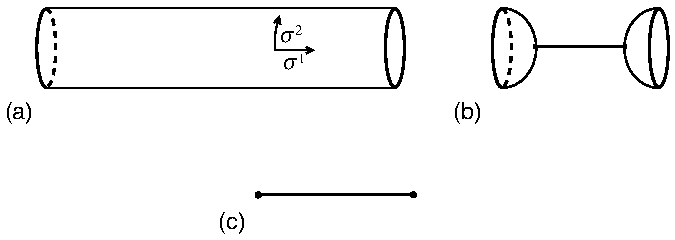
\includegraphics[width=0.8\linewidth]{figures/fig_7_1.pdf}
\caption{(a) $t$ が小さい極限の円筒。(b) 円板のタッドポール振幅と閉弦の伝播関数に分けた振幅。(c) 対応する場の理論の図。黒い丸はタッドポールを表す。}
\label{fig:7.1}
\end{figure}

円筒の $t\to\infty$ の極限は、トーラスの $\tau_2\to\infty$ の極限によく似ている。円筒は長い帯のようになり、最も軽い開弦の状態が主要な漸近挙動を与える。閉弦と同様に発散はあるが、開弦のタキオンに由来するものだけである。

$t\to0$ の極限はかなり興味深い。トーラスの場合とは異なり、積分範囲を切り取るモジュラー群の作用がないため、場の理論の UV 発散がまだ存在するように見える。しかし、弦理論のあらゆる発散と同様に、これは実際には長距離の効果として解釈すべきものであることがわかる。$t\to0$ の極限では、図\ref{fig:7.1}(a)のように円筒は非常に長くなる。つまり、閉弦が真空から現れ、ある距離を伝播してから、再び真空へ消えるように見える。このことを明確にするため、モジュラー変換(7.2.44)
\begin{equation}
\eta(it)=t^{-1/2}\eta(i/t)
\tag{7.4.2}\label{eq:7.4.2}
\end{equation}
を用い、変数を $s=\pi/t$ に変えると、
\begin{equation}
Z_{C_2}=i\frac{V_{26}n^2}{2\pi(8\pi^2\alpha')^{13}}
\int_0^\infty ds\,\eta(is/\pi)^{-24}
\tag{7.4.3}\label{eq:7.4.3}
\end{equation}
を得る。計量のスケールを $1/t$ 倍に変え、円筒の周長を通常の閉弦の周長 $2\pi$ にすると、円筒の長さは $s$ となる。
\begin{equation}
\begin{aligned}
\eta(is/\pi)^{-24}
&=\exp(2s)\prod_{n=1}^{\infty}[1-\exp(-2ns)]^{-24}\\
&=\exp(2s)+24+O(\exp(-2s))
\end{aligned}
\tag{7.4.4}\label{eq:7.4.4}
\end{equation}
と展開すると、閉弦の状態の完全系で展開したときに期待される漸近挙動が見える。言い換えると、$\sigma^2$ を世界面の時間、$\sigma^1$ を世界面の空間と考えれば、図\ref{fig:7.1}(a)は非常に短い開弦のループである。世界面の空間と時間の役割を交換すれば、境界ループから始まり、境界ループで終わる、非常に長い閉弦の世界線になる。Euclid 経路積分ではどちらの記述も使え、それぞれがモジュライ空間の異なる極限で役に立つ。

真空振幅の主要な発散は、閉弦のタキオンから生じる。これは興味の対象ではなく、解析接続によって定義できる。
\begin{equation}
\int_0^\infty ds\,\exp(\beta s)\equiv-\frac1\beta.
\tag{7.4.5}\label{eq:7.4.5}
\end{equation}
質量ゼロの閉弦の状態による第二項は、解析接続を行っても $1/0$ の形の発散を与える。この発散の起源を見るため、図\ref{fig:7.1}(b)のように過程を分けることを考えよう。第6.6節で議論したように、円板上に閉弦の頂点演算子を一つ持つ、ゼロでない振幅が存在する。このタッドポールは、閉弦が真空から現れること、あるいは真空へ消えることに対応する。二つのタッドポールの間には、閉弦の伝播関数がある。運動量空間では、質量ゼロの伝播関数は $1/k^2$ に比例する。ここでは運動量保存により、閉弦はゼロ運動量で真空から現れなければならず、そのため伝播関数は発散する。

同じ種類の発散は場の量子論にも現れる。Lagrangian に $\phi$ の一次の項を持つ、質量ゼロのスカラー場 $\phi$ を考えよう。すると、ただ一つの伝播関数につながる頂点があり、図\ref{fig:7.1}(c)の図が存在する。これは、中間の伝播関数が
\begin{equation}
\left.\frac1{k^2}\right|_{k^\mu=0}
\tag{7.4.6}\label{eq:7.4.6}
\end{equation}
であるために発散する。伝播関数の極は時空の長距離にわたる伝播と関係するので、これは長距離（IR）発散である。

場の量子論における UV 発散と IR 発散は、物理的起源が大きく異なる。UV 発散は通常、理論の破綻、ある短距離で新しい物理が必要になることを示す。IR 発散は一般に、問いの立て方が誤っているか、展開の仕方が誤っていることを意味する。ここでもそうである。通常の摂動論では、$\phi(x)=0$、あるいは他の定数の配位の周りで展開する。作用
\begin{equation}
-\frac1{g^2}\int d^dx
\left(\frac12\partial_\mu\phi\,\partial^\mu\phi+g\Lambda\phi\right)
\tag{7.4.7}\label{eq:7.4.7}
\end{equation}
に対し、運動方程式
\begin{equation}
\partial^2\phi=g\Lambda
\tag{7.4.8}\label{eq:7.4.8}
\end{equation}
は $\phi(x)=0$ を解として認めない。その代わりに、方程式\hyperref[eq:7.4.8]{(7.4.8)}の解の周りで展開しなければならない。どの解も必然的に位置に依存する。その結果得られる振幅には発散がない。右辺が摂動であるにもかかわらず（円板に適した因子 $g$ を含めてある）、こうなるのは、それが特異摂動だからである。特に、補正された背景は、ゼロ次の解の Poincaré 対称性の一部を破る。

弦理論でも状況はまったく同じである。円板のタッドポールは、ディラトンと計量の両方に対する源
\begin{equation}
-\Lambda\int d^{26}x\,(-G)^{1/2}e^{-\tilde\Phi}
\tag{7.4.9}\label{eq:7.4.9}
\end{equation}
となる。補正された場の方程式の解の周りで（計量とディラトンはもはや定数ではない）展開すれば、有限な振幅が得られる。詳細はやや複雑なので、第9章でもう少し議論する。なお、超対称な弦理論では、ツリーレベルの背景が超対称性のもとで不変であれば、通常はループ補正を受けない。

極\hyperref[eq:7.4.6]{(7.4.6)}は、ツリーレベルの振幅で出会ったものと同じ種類の発散、すなわち時空の長距離にわたる伝播に対応する共鳴である。円筒の両端に開弦の頂点演算子を加え、1ループの開弦散乱振幅を表すようにすると、一方の境界から他方へ流れる運動量 $k^\mu$ は一般にゼロでなくなる。このとき、大きい $s$ の極限\hyperref[eq:7.4.4]{(7.4.4)}には因子
\begin{equation}
\exp(-\alpha'k^2s/2)
\tag{7.4.10}\label{eq:7.4.10}
\end{equation}
が含まれ、発散は、開弦が中間状態の閉弦へ散乱することを表す運動量の極になる。したがって、第3章で述べたように、開弦理論は閉弦も含まなければならない。UV 発散を除く機構が、閉弦と開弦で異なるのは興味深い。閉弦ではモジュライ積分に対する実効的なカットオフであり、開弦では、モジュライ空間の危険な極限を長距離の現象として解釈し直すことである。

式\hyperref[eq:7.4.1]{(7.4.1)}では、$\sigma^2$ を時間として経路積分を切り開き、円筒上の経路積分を開弦のスペクトルについてのトレースに関係づけた。$\sigma^1$ を時間とすれば、閉弦の Hilbert 空間を用いて得ることもできる。$\sigma^2$ の周期を $2\pi$ とし、境界を $\sigma^1=0,s$ に置こう。閉弦は $\sigma^1=0$ である状態 $\lvert B\rangle$ として現れ、$\sigma^1=s$ で同じように消える。測度に伴う挿入を含めると、経路積分は
\begin{equation}
\langle B|c_0b_0\exp[-s(L_0+\tilde L_0)]|B\rangle
\tag{7.4.11}\label{eq:7.4.11}
\end{equation}
に比例する。境界状態 $\lvert B\rangle$ は、$\partial_1X^\mu,c^1,b_{12}$ が境界で消えるという条件で定まる。Hamiltonian 形式では、これらは $\lvert B\rangle$ を消さなければならない。Laurent 係数で書けば、
\begin{equation}
\begin{aligned}
(\alpha_n^\mu+\tilde\alpha_{-n}^\mu)|B\rangle
&=(c_n+\tilde c_{-n})|B\rangle\\
&=(b_n-\tilde b_{-n})|B\rangle=0,
\qquad\text{すべての }n
\end{aligned}
\tag{7.4.12}\label{eq:7.4.12}
\end{equation}
である。これによって
\begin{equation}
\begin{aligned}
|B\rangle\propto{}&(c_0+\tilde c_0)\\
&\times\exp\left[-\sum_{n=1}^{\infty}
\left(n^{-1}\alpha_{-n}\cdot\tilde\alpha_{-n}
+b_{-n}\tilde c_{-n}+\tilde b_{-n}c_{-n}\right)\right]|0;0\rangle
\end{aligned}
\tag{7.4.13}\label{eq:7.4.13}
\end{equation}
と定まる。これを\hyperref[eq:7.4.11]{(7.4.11)}に用いると、$\lvert B\rangle$ の規格化が未定であることを除いて、結果\hyperref[eq:7.4.3]{(7.4.3)}を得る。この表示は $t\to0$ の極限と閉弦の極を解析するのに有用である。

弦と場の理論の計算を比較することで、円板のタッドポール $\Lambda$ を決められる。ただし、次章で、より一般的な結果の特殊例として求める方が便利である。

\subsubsectionlink*{Klein の壺}

Klein の壺からの真空振幅は
\begin{equation}
\begin{aligned}
Z_{K_2}
&=\int_0^\infty\frac{dt}{4t}\operatorname{Tr}'_{\mathrm c}
\left\{\Omega\exp[-2\pi t(L_0+\tilde L_0)]\right\}\\
&=iV_d\int_0^\infty\frac{dt}{4t}(4\pi^2\alpha't)^{-d/2}
\sum_{i\in\mathcal H_{\mathrm c}^\perp}
\Omega_i\exp[-2\pi t(h_i+\tilde h_i-2)]
\end{aligned}
\tag{7.4.14}\label{eq:7.4.14}
\end{equation}
であり、記法は円筒の式\hyperref[eq:7.4.1]{(7.4.1)}に従う。向き付けのある理論のトーラスに比べ、射影演算子 $\tfrac12(1+\Omega)$ に由来する因子 $\tfrac12$ が余分にある。同じ理由で、向き付けのない理論では、トーラスと円筒の両方の振幅に余分な $\tfrac12$ が付く。これは、追加のゲージ不変性 $w\to\bar w$ に由来すると考えてもよい。平坦な26次元でトレースを評価するには、$\Omega$ の対角要素は、右向きと左向きが同じ状態にあるものだけであり、これらは $\Omega=+1$ で寄与することに注意する。するとトレースは実効的に片側だけにわたり、開弦のスペクトルと同じになる。ただし、右向きと左向きが等しい寄与をするため、共形ウェイトは二倍になる。結果は
\begin{equation}
Z_{K_2}\longrightarrow iV_{26}\int_0^\infty\frac{dt}{4t}
(4\pi^2\alpha't)^{-13}\eta(2it)^{-24}
\tag{7.4.15}\label{eq:7.4.15}
\end{equation}
である。

\begin{figure}[tbp]
\centering
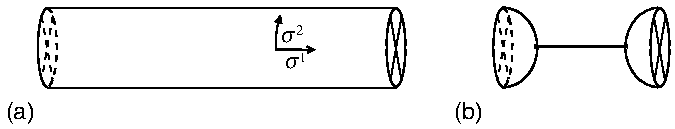
\includegraphics[width=0.8\linewidth]{figures/fig_7_2.pdf}
\caption{(a) $t$ が小さい極限の Klein の壺を、クロスキャップで両端をふさいだ円筒として表したもの。(b) $RP_2$ のタッドポール振幅と閉弦の伝播関数に分けた振幅。}
\label{fig:7.2}
\end{figure}

モジュラス $t$ は円筒と同じ範囲 $0<t<\infty$ を動くので、$t\to0$ の発散も同じである。ここでも $1/0$ の極は、閉弦の極として長距離の解釈を持つ。これを見るため、領域
\begin{align}
0\leq\sigma^1\leq2\pi,\qquad&0\leq\sigma^2\leq2\pi t,
\tag{7.4.16a}\label{eq:7.4.16a}\\
0\leq\sigma^1\leq\pi,\qquad&0\leq\sigma^2\leq4\pi t
\tag{7.4.16b}\label{eq:7.4.16b}
\end{align}
を考えよう。どちらも同一視
\begin{equation}
w\cong w+2\pi\cong-\bar w+2\pi it
\tag{7.4.17}\label{eq:7.4.17}
\end{equation}
の基本領域である。\hyperref[eq:7.4.16a]{(7.4.16a)}では、左右の辺が周期的に同一視され、上下の辺はパリティ反転の後に同一視されるため、$\Omega$ で重みを付けた閉弦のループとして解釈できる。\hyperref[eq:7.4.16b]{(7.4.16b)}については、同一視\hyperref[eq:7.4.17]{(7.4.17)}から
\begin{equation}
w\cong w+4\pi it,\qquad
w+\pi\cong-(\bar w+\pi)+2\pi it
\tag{7.4.18}\label{eq:7.4.18}
\end{equation}
も従うことに注意しよう。これより、領域\hyperref[eq:7.4.16b]{(7.4.16b)}の上下の辺は周期的に同一視される。左辺は、その長さの半分だけ平行移動し、辺に関して反射した後の自分自身と同一視される。右辺も同様であり、これはクロスキャップの定義である。したがって、図\ref{fig:7.2}(a)のように、二つのクロスキャップで両端をふさいだ円筒という表示が得られる。$1/(2t)$ 倍にスケールを変えると、円筒の周長は $2\pi$、長さは $s=\pi/(2t)$ になる。モジュラー変換の後、振幅は
\begin{equation}
Z_{K_2}=i\frac{2^{26}V_{26}}{4\pi(8\pi^2\alpha')^{13}}
\int_0^\infty ds\,\eta(is/\pi)^{-24}
\tag{7.4.19}\label{eq:7.4.19}
\end{equation}
となる。タッドポールが円板ではなく射影平面から生じることを除けば、円筒の発散についての議論がすべて当てはまる。

\subsubsectionlink*{Möbius の帯}

Möbius の帯については、
\begin{equation}
Z_{M_2}=iV_d\int_0^\infty\frac{dt}{4t}
(8\pi^2\alpha't)^{-d/2}
\sum_{i\in\mathcal H_{\mathrm o}^\perp}
\Omega_i\exp[-2\pi t(h_i-1)].
\tag{7.4.20}\label{eq:7.4.20}
\end{equation}
これは、$\Omega$ と、射影演算子に由来する因子 $\tfrac12$ だけが円筒の結果と異なる。平坦な26次元では、トレース中の演算子 $\Omega$ の効果は、偶数の質量レベルに余分な $-1$ を付け、Chan--Paton 因子を適切に数えることである。したがって、振動子のトレースは
\begin{equation}
\exp(2\pi t)\prod_{n=1}^{\infty}
[1-(-1)^n\exp(-2\pi nt)]^{-24}
=\vartheta_{00}(0,2it)^{-12}\eta(2it)^{-12}
\tag{7.4.21}\label{eq:7.4.21}
\end{equation}
となる。$SO(n)$ 理論では、$\tfrac12n(n+1)$ 個の対称な状態は $\Omega=+1$、$\tfrac12n(n-1)$ 個の反対称な状態は $\Omega=-1$ を持つので、正味の寄与は $n$ である。$Sp(k)$ 理論では、これらの縮退度が逆になり、$-n$ を与える（ここでの記法では、$Sp(k)$ は $n=2k$ 個の Chan--Paton 状態に対応することを思い出そう）。すると振幅は
\begin{equation}
Z_{M_2}=\pm inV_{26}\int_0^\infty\frac{dt}{4t}
(8\pi^2\alpha't)^{-13}
\vartheta_{00}(0,2it)^{-12}\eta(2it)^{-12}
\tag{7.4.22}\label{eq:7.4.22}
\end{equation}
である。

\begin{figure}[tbp]
\centering
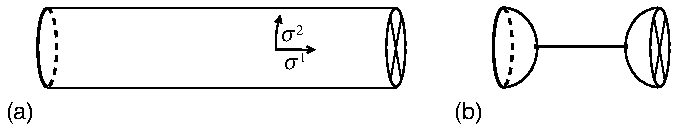
\includegraphics[width=0.8\linewidth]{figures/fig_7_3.pdf}
\caption{(a) $t$ が小さい極限の Möbius の帯を、クロスキャップを一つ付けた円筒として表したもの。(b) $D_2$ と $RP_2$ のタッドポール振幅、および閉弦の伝播関数に分けた振幅。}
\label{fig:7.3}
\end{figure}

Klein の壺と同じ構成により、Möbius の帯は、図\ref{fig:7.3}(a)のように、一端が境界で他端がクロスキャップである円筒として表せる。今度の円筒の長さは $s=\pi/(4t)$ である。モジュラー変換により、振幅は
\begin{equation}
Z_{M_2}=\pm2in\frac{2^{13}V_{26}}{4\pi(8\pi^2\alpha')^{13}}
\int_0^\infty ds\,\vartheta_{00}(0,2is/\pi)^{-12}
\eta(2is/\pi)^{-12}
\tag{7.4.23}\label{eq:7.4.23}
\end{equation}
となる。環帯の場合と同じく、これも演算子による表式に書ける。式\hyperref[eq:7.4.11]{(7.4.11)}の境界状態の一つを、同様のクロスキャップ状態 $\lvert C\rangle$ に置き換えればよい。ここでも $t\to0$ の発散があり、円板から一つ、射影平面から一つのタッドポールが生じる、図\ref{fig:7.3}(a)の過程に対応する。

向き付けのない理論では、これら三つの曲面の発散が合わさって
\begin{equation}
i\frac{24V_{26}}{4\pi(8\pi^2\alpha')^{13}}
(2^{13}\mp n)^2\int_0^\infty ds
\tag{7.4.24}\label{eq:7.4.24}
\end{equation}
となる。すなわち、全タッドポールは $2^{13}\mp n$ に比例する。ゲージ群 $SO(2^{13})=SO(8192)$ では、円板と射影平面のタッドポールが相殺して、これはゼロになる。ボソン弦ではおそらく特別な意味を持たないが、超弦理論における $SO(32)$ の同様の相殺には特別な意味がある。

\subsectionlink*{演習}
\addcontentsline{toc}{subsection}{第7章の演習}

\subsubsection*{演習7.1}\label{ex:7.1}
トーラス上の指数演算子の期待値\hyperref[eq:7.2.4]{(7.2.4)}に至る手順を補え。$\tau\to-1/\tau$ のもとで正しく変換することを示せ。

\subsubsection*{演習7.2}\label{ex:7.2}
付録Aで調和演算子について行うように、行列式を正則化して評価することにより、トーラスの真空振幅\hyperref[eq:7.3.6]{(7.3.6)}を導け。モジュラー変換が固有値を置換するだけであることを示せ。［演習A.3と比較せよ。］（参考文献：Polchinski (1986)。）

\subsubsection*{演習7.3}\label{ex:7.3}
固有関数の和(6.2.7)を実行して、Green 関数\hyperref[eq:7.2.3]{(7.2.3)}を導け。

\subsubsection*{演習7.4}\label{ex:7.4}
トーラス上の $\langle\partial_wX^\mu(w)\partial_wX_\mu(0)\rangle$ を、トレースとして表すことによって評価せよ。結果が式\hyperref[eq:7.2.16]{(7.2.16)}と一致することを示せ。

\subsubsection*{演習7.5}\label{ex:7.5}
\begin{enumerate}
\item[(a)] $\operatorname{Im}\tau\to\infty$ におけるテータ関数(7.2.37)の主要な挙動を求めよ。
\item[(b)] モジュラー変換を用い、虚軸に沿って $\tau\to0$ とするときについても同じことを行え。
\item[(c)] より風変わりな問いとして、$\tau$ が虚軸に平行な経路に沿って実軸上のゼロでない点に近づくときはどうなるか。［ヒント：その点が有理数か無理数かによって、答えは本質的に異なる。］
\end{enumerate}

\subsubsection*{演習7.6}\label{ex:7.6}
\begin{enumerate}
\item[(a)] 式\hyperref[eq:7.3.20]{(7.3.20)}、\hyperref[eq:7.3.21]{(7.3.21)}を確かめよ。
\item[(b)] 任意の次元 $d$ で、$l$ 積分にカットオフを課して $Z_{S_1}(m^2)$ を評価せよ。相殺項が $m^2$ に関して解析的であることを示せ。$d=4$ における非解析的な部分を与えよ。（参考文献：Coleman \& Weinberg (1973)。）
\end{enumerate}

\subsubsection*{演習7.7}\label{ex:7.7}
円筒上の $n$ 個の開弦タキオンの振幅を、トーラスの振幅（式\hyperref[eq:7.3.6]{(7.3.6)}と式\hyperref[eq:7.2.4]{(7.2.4)}を組み合わせたもの）と同様の形で求めよ。必要な Green 関数は、円筒をトーラスの対合として表す表示を用い、鏡像法によってトーラス上の Green 関数から得られる。

\subsubsection*{演習7.8}\label{ex:7.8}
二つの境界のそれぞれにいくつかの頂点演算子がある場合について、前問の振幅を考えよ。前問の具体的な結果から、$t\to0$ の極限が、一方の境界から他方へ流れる運動量の関数として、閉弦の極の列を与えることを示せ。

\subsubsection*{演習7.9}\label{ex:7.9}
演習6.12と7.8の両方を解いた場合、ユニタリ性が、前者の二乗を後者のタキオンの極に関係づけることを論じよ。これを用いて $g_{\mathrm c}$ と $g_{\mathrm o}^2$ の数値的な関係を求めよ。次章では、これと似たことを、より回り道をして行う。

\subsubsection*{演習7.10}\label{ex:7.10}
中間状態の開弦に関する円筒振幅のユニタリ性が、Chan--Paton 因子に
\[
\operatorname{Tr}(\lambda^a\lambda^b)\operatorname{Tr}(\lambda^c\lambda^d)
=\operatorname{Tr}(\lambda^a\lambda^b\lambda^e\lambda^c\lambda^d\lambda^e)
\]
を要求することを論じよ。ゲージ群 $U(n_1)\times U(n_2)\times\cdots\times U(n_k)$ はツリーレベルのユニタリ性と整合するが、この追加の条件は $U(n)$ を選び出すことを示せ。

\subsubsection*{演習7.11}\label{ex:7.11}
この演習は、弦理論における $D=26$ の最初の出現（Lovelace, 1971）を再現する。時空の次元を $D$、正味の振動子の組の数を $D'$ と仮定し、\hyperref[eq:7.3.9]{(7.3.9)}の形の Coleman--Weinberg 公式から円筒の真空振幅を計算せよ。頂点演算子の共形不変性が要求するとおり、タキオンの質量を $m^2=-1/\alpha'$ に保つように、開弦の質量二乗の定数項を定めよ。散乱振幅を模擬するため、式\hyperref[eq:7.4.10]{(7.4.10)}のように因子 $\exp(-\alpha'k^2s/2)$ を追加せよ。$D=26$ かつ $D'=24$ でない限り、振幅が $k^2$ に関して極ではなく分岐切断を持つことを示せ。

\subsubsection*{演習7.12}\label{ex:7.12}
前問をトーラスについて繰り返し、この場合には $D=26$ かつ $D'=24$ のときに限り、真空振幅がモジュラー不変であることを示せ（Shapiro, 1972）。

\subsubsection*{演習7.13}\label{ex:7.13}
トーラスの振幅\hyperref[eq:7.3.6]{(7.3.6)}の導出と同様の手順を実行し、弦の経路積分から Klein の壺の真空振幅\hyperref[eq:7.4.15]{(7.4.15)}を求めよ。

\subsubsection*{演習7.14}\label{ex:7.14}
境界状態\hyperref[eq:7.4.13]{(7.4.13)}を用いた振幅\hyperref[eq:7.4.11]{(7.4.11)}が、円筒の振幅\hyperref[eq:7.4.3]{(7.4.3)}を再現することを示せ。

\subsubsection*{演習7.15}\label{ex:7.15}
\begin{enumerate}
\item[(a)] クロスキャップに対応する状態 $\lvert C\rangle$ を求めよ。
\item[(b)] 式\hyperref[eq:7.4.11]{(7.4.11)}に類似した式によって、Klein の壺と Möbius の帯の真空振幅を求めよ。
\end{enumerate}

\clearpage
% 原書231--255頁（PDF253--277）、第8章導入および8.1--8.4。
\sectionlink{トーラスコンパクト化と \texorpdfstring{$T$}{T} 双対性}\label{ch:8}

弦理論の現実的なコンパクト化は第2巻の後半の章で扱うが、一つ以上の次元を周期的に同一視する、弦理論の最も簡単なコンパクト化をここで見ておくのは興味深い。まず場の理論における同じコンパクト化を考え、特にゲージ相互作用と重力の Kaluza--Klein 統一に出会う。次にこれを弦理論へ拡張する。そこでは、巻き付き状態、拡大されたゲージ対称性、$T$ 双対性、Dブレーンという、いくつかの新しい、弦に本質的な現象が生じる。また、少し複雑なコンパクト化であるオービフォールドとオリエンティフォールドも考えることになる。

\subsectionlink{場の理論におけるトーラスコンパクト化}\label{sec:8.1}

一般相対論では、時空の幾何は力学的である。私たちが見る三つの空間次元は膨張しており、かつては大きく曲がっていた。小さいままの余分な次元が存在するというのは、論理的に可能である。実際、電磁場と重力場を単一の高次元の場の成分として統一する方法として、この考えは早くも1914年に提案されていた。$x^4$ が周期的で、
\begin{equation}
x^4\cong x^4+2\pi R,
\tag{8.1.1}\label{eq:8.1.1}
\end{equation}
$\mu=0,\ldots,3$ に対する $x^\mu$ が非コンパクトな5次元理論を考える。これが\emph{トーラスコンパクト化}である。5次元計量は $G_{\mu\nu}$、$G_{\mu4}$、$G_{44}$ に分かれる。4次元の観点からは、これらは計量、ベクトル、スカラーである。

より一般に、$x^d$ が周期的な $D=d+1$ 時空次元の場合を取り、詳しく見てみよう。まだ場の理論を考えているので、$D$ は任意のままとする。計量を
\begin{equation}
ds^2=G^D_{MN}dx^Mdx^N=G_{\mu\nu}dx^\mu dx^\nu
+G_{dd}(dx^d+A_\mu dx^\mu)^2
\tag{8.1.2}\label{eq:8.1.2}
\end{equation}
とパラメータ表示する。添字 $M,N$ はすべての次元 $0,\ldots,d$ を走り、添字 $\mu,\nu$ は非コンパクトな次元 $0,\ldots,d-1$ だけを走る。完全な $D$ 次元計量を $G^D_{MN}$ と表す。$G_{\mu\nu}\ne G^D_{\mu\nu}$ であることに注意しよう。$d$ 次元の作用では、$G_{\mu\nu}$ を用いて添字を上げ下げする。今のところ、場 $G_{\mu\nu}$、$G_{dd}$、$A_\mu$ は非コンパクト座標 $x^\mu$ だけに依存してよいものとする。形 \hyperref[eq:8.1.2]{(8.1.2)} は、$x^d$ の並進のもとで不変な最も一般的な計量である。この形でも、$d$ 次元の再パラメータ化 $x'^\mu(x^\nu)$ と、再パラメータ化
\begin{equation}
x'^d=x^d+\lambda(x^\mu)
\tag{8.1.3}\label{eq:8.1.3}
\end{equation}
が許される。後者のもとでは
\begin{equation}
A'_\mu=A_\mu-\partial_\mu\lambda
\tag{8.1.4}\label{eq:8.1.4}
\end{equation}
なので、ゲージ変換が高次元の座標変換群の一部として現れる。これが \emph{Kaluza--Klein 機構}である。

$x^d$ 依存性の効果を見るため、$D$ 次元の質量ゼロのスカラー $\phi$ を考える。簡単のため、コンパクト方向の計量を $G_{dd}=1$ とする。周期的な次元の運動量は $p_d=n/R$ と量子化される。$\phi$ の $x^d$ 依存性を完全系で展開すると、
\begin{equation}
\phi(x^M)=\sum_{n=-\infty}^{\infty}\phi_n(x^\mu)\exp(inx^d/R).
\tag{8.1.5}\label{eq:8.1.5}
\end{equation}
$D$ 次元の波動方程式 $\partial_M\partial^M\phi=0$ は
\begin{equation}
\partial_\mu\partial^\mu\phi_n(x^\mu)=\frac{n^2}{R^2}\phi_n(x^\mu)
\tag{8.1.6}\label{eq:8.1.6}
\end{equation}
となる。したがって $D$ 次元の場のモード $\phi_n$ は、$n$ でラベルされる $d$ 次元の場の無限の塔になる。$d$ 次元の質量の二乗
\begin{equation}
-p^\mu p_\mu=\frac{n^2}{R^2}
\tag{8.1.7}\label{eq:8.1.7}
\end{equation}
は、$p_d$ がゼロでないすべての場についてゼロでない。$R^{-1}$ より十分低いエネルギーでは、$x^d$ に依存しない場だけが残り、物理は $d$ 次元になる。$R^{-1}$ より高いエネルギーでは、Kaluza--Klein 状態の塔が見える。

Kaluza--Klein ゲージ不変性 \hyperref[eq:8.1.3]{(8.1.3)} に対応する電荷は、運動量 $p_d$ である。この簡単な例では、Kaluza--Klein 電荷を持つすべての場に質量がある。より一般には、高スピンの場と曲がった背景があると、質量ゼロの荷電場が存在しうる。

質量ゼロの場の有効作用は、常に考察すべき重要な対象である。$G_{dd}=e^{2\sigma}$ と定義する。計量 \hyperref[eq:8.1.2]{(8.1.2)} の Ricci スカラーは
\begin{equation}
\bm R=\bm R_d-2e^{-\sigma}\nabla^2e^\sigma-\frac14e^{2\sigma}F_{\mu\nu}F^{\mu\nu},
\tag{8.1.8}\label{eq:8.1.8}
\end{equation}
ただし $\bm R$ は $G^D_{MN}$ から、$\bm R_d$ は $G_{\mu\nu}$ から構成する。重力子・ディラトン作用 \hyperref[eq:3.7.20]{(3.7.20)} は
\begin{equation}
\begin{aligned}
\bm S_1&=\frac1{2\kappa_0^2}\int d^Dx\,(-G_D)^{1/2}e^{-2\Phi}
(\bm R+4\nabla_\mu\Phi\nabla^\mu\Phi)\\
&=\frac{\pi R}{\kappa_0^2}\int d^dx\,(-G_d)^{1/2}e^{-2\Phi+\sigma}\\
&\qquad\times\left(\bm R_d-4\partial_\mu\Phi\partial^\mu\sigma
+4\partial_\mu\Phi\partial^\mu\Phi-\frac14e^{2\sigma}F_{\mu\nu}F^{\mu\nu}\right)\\
&=\frac{\pi R}{\kappa_0^2}\int d^dx\,(-G_d)^{1/2}e^{-2\Phi_d}\\
&\qquad\times\left(\bm R_d-\partial_\mu\sigma\partial^\mu\sigma
+4\partial_\mu\Phi_d\partial^\mu\Phi_d-\frac14e^{2\sigma}F_{\mu\nu}F^{\mu\nu}\right)
\end{aligned}
\tag{8.1.9}\label{eq:8.1.9}
\end{equation}
となり、すべての質量ゼロの場の運動項を与える。ここで $G_d$ は $G_{\mu\nu}$ の行列式を表し、最後の行では有効な $d$ 次元ディラトン $\Phi_d=\Phi-\sigma/2$ を導入した。ディラトンの運動項の符号が誤っているように見えるのは見かけだけである。重力子と計量のトレースとの混合も考慮する必要があるからだ。これは式 \hyperref[eq:3.7.25]{(3.7.25)} のような Weyl 変換によって最も簡単に扱え、得られる運動項は正しい符号を持つ。

場の方程式は、コンパクトな次元の半径を決めない。\footnote[1]{もちろん、物理的に非同値な解を区別するのは、不変な半径
\[
\rho=Re^\sigma
\]
だけである。$R$ を、たとえば $\alpha'^{1/2}$ のような便利な値に、あるいは無次元変数を使うなら1に固定してもよいが、一般のままにしておくと便利である。しばしば、代わりに $G_{dd}$ を1に固定する方が便利である。同様に、$\Phi$ を加法的にシフトして、$\kappa_0^2$ を $\alpha'$ の適切なべきに固定することもできるが、ここでも一般のままにしておいて支障はない。第13章では、$\Phi$ の加法的な規格化を別の方法で固定するのが自然であることを見る。}平坦な計量と定数のディラトンは、$\Phi$ と $\sigma$ の任意の値について解である。言い換えれば、$\Phi$ にも $\sigma$ にもポテンシャルエネルギーはなく、したがってこれらの場は、Goldstone ボソンとよく似て質量ゼロである。$\Phi$ と $\sigma$ の異なる値は、縮退した配位（量子論では状態）をラベルし、これらの場がゆっくり変化する状態では、エネルギーは勾配だけから生じる。Goldstone 現象との違いは、縮退した状態がいかなる対称性によっても互いに関係づけられておらず、実際に物理が $\Phi$ と $\sigma$ に依存することである。このボース理論では縮退は偶然であり、前章で議論した1ループのエネルギーが縮退を破る。超対称理論では、物理的に非同値でありながら縮退した真空の存在はごく一般的であり、力学の理解に重要な役割を果たす。非同値な真空をラベルするこれらの質量ゼロの場は、\emph{モジュライ}と呼ばれる。自然界では、超対称性の破れがほぼ確実にすべてのモジュライに質量を与えなければならない。そうでなければ、これらはほぼ重力程度の強さで無限の到達距離を持つ相互作用を媒介してしまう。第14章では、ある弦理論において、ディラトン自身が、弦の摂動論では明らかでない隠れた次元の半径であることを見る。

$A_\mu=R\widetilde A_\mu$ と定義すると、共変微分は
\begin{equation}
\partial_\mu+ip_dA_\mu=\partial_\mu+in\widetilde A_\mu
\tag{8.1.10}\label{eq:8.1.10}
\end{equation}
となり、電荷は整数になる。$d$ 次元のゲージ結合と重力結合は、通常、次のように定義する。Lagrangian 密度の $\widetilde F_{\mu\nu}\widetilde F^{\mu\nu}$ の係数を $-1/(4g_d^2)$、$\bm R_d$ の係数を $1/(2\kappa_d^2)$ と定義する。したがってゲージ結合は、重力結合によって
\begin{equation}
g_d^2=\frac{\kappa_0^2e^{2\Phi_d}}{\pi R^3e^{2\sigma}}
=\frac{2\kappa_d^2}{\rho^2}
\tag{8.1.11}\label{eq:8.1.11}
\end{equation}
と決まる。$d$ 次元と $D$ 次元の重力結合は
\begin{equation}
\frac1{\kappa_d^2}=\frac{2\pi\rho}{\kappa^2}
\tag{8.1.12}\label{eq:8.1.12}
\end{equation}
で関係づけられ、$2\pi\rho$ はコンパクト化された次元の体積である。

反対称テンソルも、Kaluza--Klein 機構の一般化によってゲージ対称性を生む。$B_{MN}$ を $B_{\mu\nu}$ と $A'_\mu=B_{d\mu}$ に分けると、式 \hyperref[eq:3.7.7]{(3.7.7)} で定義したゲージパラメータ $\zeta_M$ は、$d$ 次元の反対称テンソル変換 $\zeta_\mu$ と、通常のゲージ不変性 $\zeta_d$ に分かれる。ゲージ場は $B_{d\mu}$、場の強さは $H_{d\mu\nu}$ である。反対称テンソルの作用は
\begin{equation}
\begin{aligned}
\bm S_2&=-\frac1{24\kappa_0^2}\int d^Dx\,(-G_D)^{1/2}e^{-2\Phi}H_{MNL}H^{MNL}\\
&=-\frac{\pi R}{12\kappa_0^2}\int d^dx\,(-G_d)^{1/2}e^{-2\Phi_d}
\left(\widetilde H_{\mu\nu\lambda}\widetilde H^{\mu\nu\lambda}
+3e^{-2\sigma}H_{d\mu\nu}H_d{}^{\mu\nu}\right)
\end{aligned}
\tag{8.1.13}\label{eq:8.1.13}
\end{equation}
となる。ここで
\begin{equation}
\widetilde H_{\mu\nu\lambda}=(\partial_\mu B_{\nu\lambda}-A_\mu H_{d\nu\lambda})
+\text{巡回置換項}
\tag{8.1.14}\label{eq:8.1.14}
\end{equation}
と定義した。ベクトルポテンシャルに比例する項は、逆計量 $G^{MN}$ から生じる。これは \emph{Chern--Simons 項}と呼ばれる。この名称は、一つのゲージポテンシャルと任意個の場の強さを反対称化して組み合わせたものを意味する。このような項は超対称理論のさまざまな場所に現れ、興味深い物理的効果と結び付いている。特に、$A_\mu$ の変換 \hyperref[eq:8.1.4]{(8.1.4)} が、変換
\begin{equation}
B'_{\nu\lambda}=B_{\nu\lambda}-\lambda H_{d\nu\lambda}
\tag{8.1.15}\label{eq:8.1.15}
\end{equation}
によって相殺されるため、$\widetilde H_{\mu\nu\lambda}$ がゲージ不変であることに注意しよう。

ポテンシャル $B_{MN}$ を他の場に最小結合させる方法はない。したがって Kaluza--Klein の場合とは異なり、反対称テンソルのゲージ対称性のもとで電荷を持つ場は存在しない。この点は弦理論では異なる。

\subsectionlink{CFT におけるトーラスコンパクト化}\label{sec:8.2}

次に、一つの周期的なスカラー場
\begin{equation}
X\cong X+2\pi R
\tag{8.2.1}\label{eq:8.2.1}
\end{equation}
の共形場理論を考える。式を煩雑にしないため、$X^d$ の上添字を省き、$G_{dd}=1$ と置く。世界面の作用は非コンパクトな理論と同じ $\int d^2z\,\partial X\bar\partial X/(2\pi\alpha')$ なので、運動方程式、演算子積、エネルギー運動量テンソルは変わらない。特に、この理論は依然として共形不変である。周期性には二つの効果がある。第一に、弦の状態は同一視 \hyperref[eq:8.2.1]{(8.2.1)} のもとで一価でなければならない。すなわち、周期的な次元を一周するよう弦を並進させる演算子 $\exp(2\pi iRp)$ は状態を不変に保たなければならないので、重心運動量が
\begin{equation}
k=\frac nR,\qquad n\in\mathbb Z
\tag{8.2.2}\label{eq:8.2.2}
\end{equation}
と量子化される。これは場の理論と同じである。

第二の効果は弦理論に特有である。今度は閉弦がコンパクト方向に巻き付くことができる：
\begin{equation}
X(\sigma+2\pi)=X(\sigma)+2\pi Rw,\qquad w\in\mathbb Z.
\tag{8.2.3}\label{eq:8.2.3}
\end{equation}
整数 $w$ は\emph{巻き付き数}である。巻き付き数 $+1$、$0$、$-1$ の状態を図\ref{fig:8.1}(a) に示した。世界面の場の理論の観点からは、巻き付き数がゼロでない弦は、位相的に非自明な場の配位を持つ状態、すなわち\emph{位相的ソリトン}である。整合的な弦理論は、巻き付き数を持つ状態を含まなければならない。図\ref{fig:8.1}(b) のように、通常の分裂・結合過程によって、$w=0$ の弦が $w=+1$ と $w=-1$ の対に変わりうるからである。この例のように、巻き付き数が常に保存することは容易に分かる。

\begin{figure}[htbp]
\centering
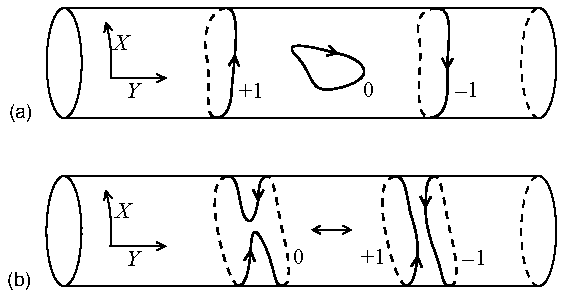
\includegraphics[width=0.9\linewidth]{figures/fig_8_1.pdf}
\caption{(a) 巻き付き数 $w=+1,0,-1$ の向き付き閉弦。説明のため、コンパクトな次元 $X$ を一つ、非コンパクトな次元 $Y$ を一つ示している。(b) $w=0$ の弦から、$w=+1$ および $w=-1$ の弦への遷移。}\label{fig:8.1}
\end{figure}

閉弦 CFT の状態を記述するため、Laurent 展開
\begin{equation}
\partial X(z)=-i\left(\frac{\alpha'}2\right)^{1/2}\sum_{m=-\infty}^{\infty}\frac{\alpha_m}{z^{m+1}},
\qquad
\bar\partial X(\bar z)=-i\left(\frac{\alpha'}2\right)^{1/2}\sum_{m=-\infty}^{\infty}\frac{\widetilde\alpha_m}{\bar z^{m+1}}
\tag{8.2.4}\label{eq:8.2.4}
\end{equation}
を考える。弦を一周するときの座標 $X$ の全変化は
\begin{equation}
2\pi Rw=\oint(dz\,\partial X+d\bar z\,\bar\partial X)
=2\pi(\alpha'/2)^{1/2}(\alpha_0-\widetilde\alpha_0).
\tag{8.2.5}\label{eq:8.2.5}
\end{equation}
全 Noether 運動量は
\begin{equation}
p=\frac1{2\pi\alpha'}\oint(dz\,\partial X-d\bar z\,\bar\partial X)
=(2\alpha')^{-1/2}(\alpha_0+\widetilde\alpha_0).
\tag{8.2.6}\label{eq:8.2.6}
\end{equation}
非コンパクトな次元なら、通常の関係 $\alpha_0=\widetilde\alpha_0=p(\alpha'/2)^{1/2}$ が得られるが、周期的な次元では
\begin{align}
p_L&\equiv(2/\alpha')^{1/2}\alpha_0=\frac nR+\frac{wR}{\alpha'},
\tag{8.2.7a}\label{eq:8.2.7a}\\
p_R&\equiv(2/\alpha')^{1/2}\widetilde\alpha_0=\frac nR-\frac{wR}{\alpha'}.
\tag{8.2.7b}\label{eq:8.2.7b}
\end{align}
Virasoro 生成子は
\begin{align}
L_0&=\frac{\alpha'p_L^2}4+\sum_{n=1}^{\infty}\alpha_{-n}\alpha_n,
\tag{8.2.8a}\label{eq:8.2.8a}\\
\widetilde L_0&=\frac{\alpha'p_R^2}4+\sum_{n=1}^{\infty}\widetilde\alpha_{-n}\widetilde\alpha_n.
\tag{8.2.8b}\label{eq:8.2.8b}
\end{align}

\subsubsectionlink*{分配関数}

$X$ の分配関数は今度は
\begin{equation}
\begin{aligned}
(q\bar q)^{-1/24}\operatorname{Tr}(q^{L_0}\bar q^{\widetilde L_0})
&=|\eta(\tau)|^{-2}\sum_{n,w=-\infty}^{\infty}
q^{\alpha'p_L^2/4}\bar q^{\alpha'p_R^2/4}\\
&=|\eta(\tau)|^{-2}\sum_{n,w=-\infty}^{\infty}
\exp\left[-\pi\tau_2\left(\frac{\alpha'n^2}{R^2}+\frac{w^2R^2}{\alpha'}\right)+2\pi i\tau_1nw\right].
\end{aligned}
\tag{8.2.9}\label{eq:8.2.9}
\end{equation}
振動子の和は非コンパクトな場合と同じだが、運動量積分は $n$ と $w$ の和に置き換わる。モジュラー不変性は明白ではないが、Poisson 再総和公式
\begin{equation}
\sum_{n=-\infty}^{\infty}\exp(-\pi an^2+2\pi ibn)
=a^{-1/2}\sum_{m=-\infty}^{\infty}\exp\left[-\frac{\pi(m-b)^2}{a}\right]
\tag{8.2.10}\label{eq:8.2.10}
\end{equation}
を使えば明白にできる。分配関数は
\begin{equation}
2\pi RZ_X(\tau)\sum_{m,w=-\infty}^{\infty}
\exp\left(-\frac{\pi R^2|m-w\tau|^2}{\alpha'\tau_2}\right)
\tag{8.2.11}\label{eq:8.2.11}
\end{equation}
となる。ここで $Z_X(\tau)$ は非コンパクトな理論のモジュラー不変な表式 \hyperref[eq:7.2.9]{(7.2.9)} である。変数を $m\to m+w$ と変えれば、この和は明らかに $\tau\to\tau+1$ のもとで不変である。また、$m\to-w$、$w\to m$ とすれば、$\tau\to-1/\tau$ のもとでも不変である。

表式 \hyperref[eq:8.2.11]{(8.2.11)} には簡単な経路積分による解釈がある。周期的な時空で種数1のすべての世界面について和を取るとき、世界面上の各非自明な閉曲線はコンパクト方向に巻き付くことができる：
\begin{align}
X(\sigma^1+2\pi,\sigma^2)&=X(\sigma^1,\sigma^2)+2\pi wR,
\tag{8.2.12a}\label{eq:8.2.12a}\\
X(\sigma^1+2\pi\tau_1,\sigma^2+2\pi\tau_2)&=X(\sigma^1,\sigma^2)+2\pi mR.
\tag{8.2.12b}\label{eq:8.2.12b}
\end{align}
すなわち、経路積分は $w$ と $m$ でラベルされる位相的に異なるセクターに分かれる。Gaussian 経路積分は、$X$ を正しい周期性を持つ古典解
\begin{equation}
X_{\mathrm{cl}}=\sigma^1wR+\sigma^2(m-w\tau_1)R/\tau_2
\tag{8.2.13}\label{eq:8.2.13}
\end{equation}
と、周期境界条件を満たす量子的な部分との和として書く、通常の方針で実行できる。作用は古典的な部分と量子的な部分に分かれる。量子的な部分の経路積分は非コンパクトな場合と同じであり、古典作用は式 \hyperref[eq:8.2.11]{(8.2.11)} の指数に現れる。このとき、モジュラー変換が周期性に及ぼす効果は、単に和の変数 $m,w$ の変更となる。

\subsubsectionlink*{頂点演算子}

$\alpha_0\ne\widetilde\alpha_0$ となる巻き付き状態を作るには、
\begin{equation}
[x_L,p_L]=[x_R,p_R]=i
\tag{8.2.14}\label{eq:8.2.14}
\end{equation}
を満たす独立な変数 $x_L,x_R$ が必要である。このとき場 $X$ は正則部分と反正則部分に分かれる：
\begin{equation}
X(z,\bar z)=X_L(z)+X_R(\bar z),
\tag{8.2.15}\label{eq:8.2.15}
\end{equation}
ただし
\begin{align}
X_L(z)&=x_L-i\frac{\alpha'}2p_L\ln z
+i\left(\frac{\alpha'}2\right)^{1/2}\sum_{\substack{m=-\infty\\m\ne0}}^{\infty}\frac{\alpha_m}{mz^m},
\tag{8.2.16a}\label{eq:8.2.16a}\\
X_R(\bar z)&=x_R-i\frac{\alpha'}2p_R\ln\bar z
+i\left(\frac{\alpha'}2\right)^{1/2}\sum_{\substack{m=-\infty\\m\ne0}}^{\infty}\frac{\widetilde\alpha_m}{m\bar z^m}.
\tag{8.2.16b}\label{eq:8.2.16b}
\end{align}
$k_L=k_R$ の状態と、和 $X_L(z)+X_R(\bar z)$ だけから構成した演算子に注目すれば、これは非コンパクトな次元の CFT に帰着する。

OPE と頂点演算子について、まず多少発見法的に議論し、その後で詳細を補おう。通常の $XX$ 演算子積 $-(\alpha'/2)\ln(z_{12}\bar z_{12})$ が正則関数と反正則関数の和に分かれるので、演算子積がどうなるべきかは容易に推測できる。したがって、
\begin{align}
X_L(z_1)X_L(z_2)&\sim-\frac{\alpha'}2\ln z_{12},\qquad
X_R(\bar z_1)X_R(\bar z_2)\sim-\frac{\alpha'}2\ln\bar z_{12},
\tag{8.2.17a}\label{eq:8.2.17a}\\
X_L(z_1)X_R(\bar z_2)&\sim0.
\tag{8.2.17b}\label{eq:8.2.17b}
\end{align}
状態 $\lvert0;k_L,k_R\rangle$ に対応する演算子は
\begin{equation}
\mathcal V_{k_Lk_R}(z,\bar z)=:e^{ik_LX_L(z)+ik_RX_R(\bar z)}:
\tag{8.2.18}\label{eq:8.2.18}
\end{equation}
となり、その OPE は
\begin{equation}
\mathcal V_{k_Lk_R}(z_1,\bar z_1)\mathcal V_{k'_Lk'_R}(z_2,\bar z_2)
\sim z_{12}^{\alpha'k_Lk'_L/2}\bar z_{12}^{\alpha'k_Rk'_R/2}
\mathcal V_{(k+k')_L(k+k')_R}(z_2,\bar z_2)
\tag{8.2.19}\label{eq:8.2.19}
\end{equation}
である。さまざまな表式に分岐切断が現れるが、場 $X$ はもはや一価ではないので、これは驚くことではない。しかし、頂点演算子の完全な OPE が一価であることは重要である。$z_1$ が $z_2$ を一周したときの正味の位相は
\begin{equation}
\exp[\pi i\alpha'(k_Lk'_L-k_Rk'_R)]
=\exp[2\pi i(nw'+wn')]=1.
\tag{8.2.20}\label{eq:8.2.20}
\end{equation}
弦の振幅が適切に定義されるためには、こうでなければならない。

\subsubsectionlink*{技術的な注意}

以上は本質的に正しいが、対数の分岐切断の位置については無頓着であった。点 $z_1,z_2$ と運動量 $k,k'$ を交換すると、OPE \hyperref[eq:8.2.19]{(8.2.19)} に問題があることが分かる。左辺は対称だが、右辺は $\exp[\pi i(nw'+wn')]$ だけ変わるので、$nw'+wn'$ が奇数なら符号が変わる。この問題は次のようにも見て取れる。モード展開から、等時刻（$|z_1|=|z_2|$）の交換子
\begin{equation}
[X_L(z_1),X_L(z_2)]=\frac{\pi i\alpha'}2\operatorname{sign}(\sigma_1^1-\sigma_2^1)
\tag{8.2.21}\label{eq:8.2.21}
\end{equation}
を導ける。CBH 公式によれば、演算子を単に生成・消滅演算子の正規順序で定義すると、$nw'+wn'$ が奇数のとき、演算子 $\mathcal V_{k_Lk_R}$ と $\mathcal V_{k'_Lk'_R}$ は交換する代わりに反交換する。見えなかった分岐切断 \hyperref[eq:8.2.20]{(8.2.20)} が、二つの見える分岐切断に分かれてしまう。頂点演算子の正しい振動子表示は（位相には多少の任意性がある）、
\begin{equation}
\mathcal V_{k_Lk_R}(z,\bar z)
=\exp[\pi i(k_L-k_R)(p_L+p_R)\alpha'/4]
\canorm{e^{ik_LX_L(z)+ik_RX_R(\bar z)}}
\tag{8.2.22}\label{eq:8.2.22}
\end{equation}
である。通常どおり $p$ は運動量演算子、$k$ は数（その頂点演算子が運ぶ運動量）である。$\mathcal V_{k_Lk_R}$ と $\mathcal V_{k'_Lk'_R}$ の順序を交換すると、\emph{コサイクル}と呼ばれる追加の因子が、さらに位相
\begin{equation}
\begin{aligned}
&\exp\left\{\pi i\bigl[(k_L-k_R)(k'_L+k'_R)
-(k'_L-k'_R)(k_L+k_R)\bigr]\alpha'/4\right\}\\
&\qquad=\exp[\pi i(nw'-wn')]
\end{aligned}
\tag{8.2.23}\label{eq:8.2.23}
\end{equation}
を与え、分岐切断を取り除く。大抵の目的では、この複雑さを無視し、前の段落のより簡単な表式を使ってよい。コサイクルは、一部の振幅の相対的な符号だけに影響する。

一般的な $X^\mu$ 経路積分 \hyperref[eq:6.2.18]{(6.2.18)} は、正則部分と反正則部分の積に明らかな仕方で因数分解するので、単に
\begin{equation}
\prod_{\substack{i,j=1\\i<j}}^n|z_{ij}|^{\alpha'k_ik_j}
\ \longrightarrow\
\prod_{\substack{i,j=1\\i<j}}^n
z_{ij}^{\alpha'k_{Li}k_{Lj}/2}\bar z_{ij}^{\alpha'k_{Ri}k_{Rj}/2}
\tag{8.2.24}\label{eq:8.2.24}
\end{equation}
と置き換え、さらに $x_0$ の非コンパクトな積分から生じる $2\pi\delta(\sum k)$ を
\begin{equation}
2\pi R\delta_{\sum_i n_i,0}\delta_{\sum_i w_i,0}
\tag{8.2.25}\label{eq:8.2.25}
\end{equation}
で置き換えればよい。ここでもこれは素朴な扱いであり、正確な表式 \hyperref[eq:8.2.22]{(8.2.22)} は、さらにいくつかの符号を与える。読者は四つの頂点演算子を含む振幅を容易に計算できる。それは Virasoro--Shapiro 振幅に似ている。

\subsubsectionlink*{DDF 演算子}

指数関数演算子を正則部分と反正則部分に分離できることを見た。これには多くの応用がある。ここでは、第4章の終わりで残しておいた DDF 演算子の問題を片づけるために使う。

光円錐座標 $X^\pm=2^{-1/2}(X^0\pm X^1)$ を用いる。その正則部分の OPE は（添字 $L$ を省く）
\begin{equation}
X^+(z)X^-(0)\sim\frac{\alpha'}2\ln z,\qquad
X^+(z)X^+(0)\sim X^-(z)X^-(0)\sim0.
\tag{8.2.26}\label{eq:8.2.26}
\end{equation}
したがって、$i$ を横方向として、演算子
\begin{equation}
V^i(nk_0,z)=\partial X^i(z)e^{ink_0X^+(z)}(2/\alpha')^{1/2}
\tag{8.2.27}\label{eq:8.2.27}
\end{equation}
は $(1,0)$ の一次場であり、OPE は
\begin{equation}
\begin{aligned}
V^i(nk_0,z)V^j(mk_0,0)&\sim-\frac{\delta^{ij}}{z^2}e^{i(n+m)k_0X^+(0)}\\
&\quad-\frac{ink_0\delta^{ij}}z\partial X^+(0)e^{i(n+m)k_0X^+(0)}.
\end{aligned}
\tag{8.2.28}\label{eq:8.2.28}
\end{equation}
DDF 演算子を
\begin{equation}
A_n^i=\oint\frac{dz}{2\pi}V^i(nk_0,z)
\tag{8.2.29}\label{eq:8.2.29}
\end{equation}
と定義する。OPE \hyperref[eq:8.2.28]{(8.2.28)} の $z^{-1}$ の項の留数は、$n+m=0$ の場合を除いて全微分である。したがって DDF 演算子は
\begin{equation}
[A_m^i,A_n^j]=m\delta^{ij}\delta_{m,-n}\frac{\alpha'k_0p^+}{2}
\tag{8.2.30}\label{eq:8.2.30}
\end{equation}
を満たし、これは規格化を除いて振動子代数である。

運動量 $q$ の状態に対する DDF 演算子の作用を考える。$V^i(nk_0,z)$ とこの状態の頂点演算子との OPE には $z^{-\alpha'nk_0q^-/2}$ が現れるので、$k_0=2/(\alpha'q^-)$ と固定すれば一価になる。このとき周回積分 \hyperref[eq:8.2.29]{(8.2.29)} は、このセクターで意味のある演算子を定義する。DDF 演算子は $(1,0)$ テンソルの積分なので、Virasoro 生成子と可換であり、物理状態を物理状態へ写す。したがって、振動子の基底状態に DDF 演算子を作用させて物理状態を作れる。このようにして得られる状態は光円錐状態と一対一に対応するので、物理状態の完全系となる。DDF 演算子は $X^-$ を含まないので、これらの状態には $\alpha^-_{-m}$ の励起がない。したがって、これらは、より一般的だが明示性に乏しい構成 \hyperref[eq:4.4.19]{(4.4.19)} で与えた状態と同じである。

\subsectionlink{閉弦と \texorpdfstring{$T$}{T} 双対性}\label{sec:8.3}

ここからは弦理論を考えるので $D=26$ とし、まず $X^{25}$ だけを周期的とする。質量殻条件（$L_0$ と $\widetilde L_0$ の条件）は
\begin{equation}
\begin{aligned}
m^2=-k^\mu k_\mu&=(k_L^{25})^2+\frac4{\alpha'}(N-1)\\
&=(k_R^{25})^2+\frac4{\alpha'}(\widetilde N-1),
\end{aligned}
\tag{8.3.1}\label{eq:8.3.1}
\end{equation}
あるいは
\begin{align}
m^2&=\frac{n^2}{R^2}+\frac{w^2R^2}{\alpha'^2}
+\frac2{\alpha'}(N+\widetilde N-2),
\tag{8.3.2a}\label{eq:8.3.2a}\\
0&=nw+N-\widetilde N.
\tag{8.3.2b}\label{eq:8.3.2b}
\end{align}
質量の二乗には、コンパクト方向の運動量、巻き付いた弦のポテンシャルエネルギー、振動子、零点エネルギーという四つの寄与がある。第4章の物理的スペクトルの議論は任意のコンパクト化に対して有効だったので、横方向の振動子 $M=2,\ldots,25$ だけを考えれば、状態を正しく数えられる。

まず、質量ゼロのスペクトルについて場の理論の結果を再現しよう。一般的な $R$ の値では、状態が質量ゼロになる唯一の方法は $n=w=0$、$N=\widetilde N=1$ である。これらは非コンパクトな理論と同じ $24^2$ 個の状態だが、ここでは振動が時空方向 $\mu$ にあるか、内部方向25にあるかに従って分けると便利である：
\begin{equation}
\begin{gathered}
\alpha_{-1}^\mu\widetilde\alpha_{-1}^\nu\lvert0;k\rangle,
\qquad (\alpha_{-1}^\mu\widetilde\alpha_{-1}^{25}+\alpha_{-1}^{25}\widetilde\alpha_{-1}^\mu)\lvert0;k\rangle,\\
(\alpha_{-1}^\mu\widetilde\alpha_{-1}^{25}-\alpha_{-1}^{25}\widetilde\alpha_{-1}^\mu)\lvert0;k\rangle,
\qquad\alpha_{-1}^{25}\widetilde\alpha_{-1}^{25}\lvert0;k\rangle.
\end{gathered}
\tag{8.3.3}\label{eq:8.3.3}
\end{equation}
最初の状態は、さらに25次元の重力子、ディラトン、反対称テンソルに分かれる。第2の状態は、時空添字一つと内部添字一つを持つ重力子であり、Kaluza--Klein ベクトルである。第3の状態は、反対称テンソルから生じるベクトルである。最後の状態はスカラーであり、コンパクト方向の半径のモジュラスである。その頂点演算子 $:\partial X^{25}\bar\partial X^{25}e^{ik\cdot X}:$ は、計量 $G_{25,25}$ の摂動である。これは低エネルギーの場の理論を考えて得たものと同じ質量ゼロのスペクトルである。

$U(1)\times U(1)$ 対称性のもとでの有質量状態の電荷を考えるのは興味深い。Kaluza--Klein ゲージ対称性は、ここでも $X^{25}$ の並進から生じるので、対応する電荷はコンパクト方向の運動量 $p^{25}$ である。反対称テンソルのゲージ対称性については、運動量ゼロの頂点演算子を考える。これは、結合する任意の状態の電荷を測る。その演算子は
\begin{equation}
\partial X^\mu\bar\partial X^{25}-\partial X^{25}\bar\partial X^\mu
=\bar\partial(X^{25}\partial X^\mu)-\partial(X^{25}\bar\partial X^\mu)
\tag{8.3.4}\label{eq:8.3.4}
\end{equation}
に比例する。これは全微分だが、巻き付き状態では $X^{25}$ が一価でないため、積分してもゼロにはならない。したがって $B_{\mu,25}$ の電荷は巻き付き数である。これは、このコンパクト化に現れる「弦的」な物理のいくつかの例の最初のものである。場の理論には、この電荷を持つ状態がなかった。

弦の3点結合からゲージ結合を明示的に確かめよう。ゲージボソンの頂点演算子は
\begin{equation}
\frac{2^{1/2}g_{\mathrm c,25}}{\alpha'}:
(\partial X^\mu\bar\partial X^{25}\pm\partial X^{25}\bar\partial X^\mu)e^{ik\cdot X}:.
\tag{8.3.5}\label{eq:8.3.5}
\end{equation}
25次元の弦結合定数を $g_{\mathrm c,25}=g_{\mathrm c}(2\pi R)^{-1/2}$ と定義した。因子 $(2\pi R)^{-1/2}$ はゼロモードの波動関数の規格化から生じる。一般的なコンパクト運動量と巻き付きを持つタキオンの頂点演算子は
\begin{equation}
g_{\mathrm c,25}:e^{ik_L\cdot X_L(z)+ik_R\cdot X_R(\bar z)}:.
\tag{8.3.6}\label{eq:8.3.6}
\end{equation}
一つのゲージボソンと二つのタキオンの3点振幅で、タキオンがゼロでないコンパクト運動量と巻き付きを持つ場合は、式 \hyperref[eq:6.6.14]{(6.6.14)} と同様であり、
\begin{equation}
\begin{aligned}
&-2^{-1/2}\pi ig_{\mathrm c,25}(2\pi)^{25}\delta^{25}\!\left(\sum_i k_i\right)
k_{23}^\mu(k_{L23}^{25}\pm k_{R23}^{25})\\
&\quad\longrightarrow-2^{3/2}\pi ig_{\mathrm c,25}(2\pi)^{25}\delta^{25}\!\left(\sum_i k_i\right)
k_2^\mu(k_{L2}^{25}\pm k_{R2}^{25}).
\end{aligned}
\tag{8.3.7}\label{eq:8.3.7}
\end{equation}
第2行ではゲージボソンの運動量を $k_1\to0$ とし、これによってゲージ結合を定義した。したがって、二つのゲージボソンはそれぞれ $k_{L2}^{25}\pm k_{R2}^{25}$、すなわち予想どおりコンパクト運動量と巻き付きに結合する。ゲージボソンを重力子に置き換えた振幅も考えれば、有効作用から得たものと同じ、さまざまな結合の間の関係 \hyperref[eq:8.1.11]{(8.1.11)}、\hyperref[eq:8.1.12]{(8.1.12)} を再現できる。

\subsubsectionlink*{拡大されたゲージ対称性}

ここまでの内容は、一つのコンパクト次元を持つ場の理論の場合とほぼ完全に同じである。26次元の重力子から25次元の重力子、ベクトル、モジュラスが生じる、といった具合である。弦に特有の効果は、巻き付き状態が $B_{\mu,25}$ の電荷を持つことだけであった。

特別なコンパクト化半径では、さらに著しい効果が生じる。これまでの質量ゼロのスペクトルの議論では、半径 $R$ の特定の値でのみ質量ゼロとなる状態を省いていた。最も豊富な構造を持つのは $R=\alpha'^{1/2}$ の場合であり、$k_{L,R}^{25}=(n\pm w)\alpha'^{-1/2}$ となって、質量ゼロの状態の条件は
\begin{equation}
(n+w)^2+4N=(n-w)^2+4\widetilde N=4
\tag{8.3.8}\label{eq:8.3.8}
\end{equation}
である。一般的な解 $n=w=0$、$N=\widetilde N=1$ に加えて、今度は
\begin{equation}
n=w=\pm1,\quad N=0,\quad\widetilde N=1,
\qquad n=-w=\pm1,\quad N=1,\quad\widetilde N=0
\tag{8.3.9}\label{eq:8.3.9}
\end{equation}
および
\begin{equation}
n=\pm2,\quad w=N=\widetilde N=0,
\qquad w=\pm2,\quad n=N=\widetilde N=0
\tag{8.3.10}\label{eq:8.3.10}
\end{equation}
もある。

状態 \hyperref[eq:8.3.9]{(8.3.9)} には、頂点演算子
\begin{equation}
:\bar\partial X^\mu e^{ik\cdot X}\exp[\pm2i\alpha'^{-1/2}X_L^{25}]:,
\qquad :\partial X^\mu e^{ik\cdot X}\exp[\pm2i\alpha'^{-1/2}X_R^{25}]:
\tag{8.3.11}\label{eq:8.3.11}
\end{equation}
を持つ四つの新しいゲージボソンが含まれる。指数関数演算子の正確な定義は、前節で議論したとおりである。これらの状態は内部運動量と巻き付き数を持つので、Kaluza--Klein および反対称テンソルのゲージ電荷を運ぶ。荷電した質量ゼロのベクトルの整合的な理論は非 Abel ゲージ理論しかないため、新しいゲージボソンは以前のものと組み合わさって非 Abel 理論を形成しなければならない。ここで、以前のベクトルについては $\partial X^{25}\bar\partial X^\mu$ と $\partial X^\mu\bar\partial X^{25}$ という基底を使うと便利である。前者は $k_L^{25}$ に結合し、そのもとで \hyperref[eq:8.3.11]{(8.3.11)} の最初の対の状態は電荷 $\pm1$ を持ち、第2の対は中性である。後者は同様に $k_R^{25}$ に結合するので、もう一方の対に結合する。これにより、ゲージ群は $SU(2)\times SU(2)$ と同定される。$\bar\partial X^\mu$ を含む三つのベクトルが一方の $SU(2)$ を形成し、$\partial X^\mu$ を含む三つがもう一方を形成する。

$SU(2)\times SU(2)$ を明示するため、三つの $(1,0)$ カレントを定義する：
\begin{align}
j^1(z)&=:\cos[2\alpha'^{-1/2}X_L^{25}(z)]:,
\tag{8.3.12a}\label{eq:8.3.12a}\\
j^2(z)&=:\sin[2\alpha'^{-1/2}X_L^{25}(z)]:,
\tag{8.3.12b}\label{eq:8.3.12b}\\
j^3(z)&=i\partial X_L^{25}(z)/\alpha'^{1/2}.
\tag{8.3.12c}\label{eq:8.3.12c}
\end{align}
これらは OPE が
\begin{equation}
j^i(z)j^j(0)\sim\frac{\delta^{ij}}{2z^2}+i\frac{\epsilon^{ijk}}zj^k(0)
\tag{8.3.13}\label{eq:8.3.13}
\end{equation}
となるよう規格化してある。もちろん、$(0,1)$ のカレント $\widetilde j^i$ にも同様の OPE がある。単純極の項は、対応する電荷が $SU(2)$ 代数をなすことを意味する。実際には、カレントが正則なので、Laurent 係数によって無限次元代数が形成される：
\begin{align}
j^i(z)&=\sum_{m=-\infty}^{\infty}\frac{j_m^i}{z^{m+1}},
\tag{8.3.14a}\label{eq:8.3.14a}\\
[j_m^i,j_n^j]&=\frac m2\delta_{m,-n}\delta^{ij}+i\epsilon^{ijk}j_{m+n}^k.
\tag{8.3.14b}\label{eq:8.3.14b}
\end{align}
これは\emph{カレント代数}、\emph{アフィン Lie 代数}、あるいは \emph{Kac--Moody 代数}などと呼ばれる。第11章以降では、このような代数を広く扱う。$z^{-2}$ の項の係数は量子化され、\hyperref[eq:8.3.13]{(8.3.13)} の値が最小であることが示されるので、これは\emph{レベル1}の $SU(2)$ カレント代数と呼ばれる。

この $SU(2)\times SU(2)$ 対称性の存在は、弦理論が時空の幾何を見る仕方が、私たちになじみのある場の理論とは異なることを示す最初の兆候である。場の理論では、どの半径でも明らかなのは $U(1)\times U(1)$ 対称性だけである。$j^3$ と $j^{1,2}$ のカレントは、それぞれ振動子励起と巻き付き・運動量励起という、まったく異なる起源を持つように見え、$X^{25}$ による表式も大きく異なるが、弦スペクトルへの作用においては対称性で互いに関係づけられている。余分なベクトルが質量ゼロなのは、内部運動量と巻き付きのエネルギーが、負の零点エネルギーによって相殺されるためである。そのため読者は、これらがタキオンを持つ理論でしか生じないのではないかと思うかもしれないが、第2巻ではそうではないことを見る。

\subsubsectionlink*{スケールと結合}

$SU(2)\times SU(2)$ の半径では、関係 \hyperref[eq:8.1.11]{(8.1.11)} は\footnote[2]{正確には、これは $(n,w)=(1,0)$ の状態の結合であった。非 Abel ゲージボソンは $(|n|,|w|)=(1,1)$ を持つので、その結合は $g_{SU(2),25}^2=4\kappa_{25}^2/\alpha'$ であり、これが素粒子物理で通常用いる $SU(2)$ 結合の定義である。第18章では、これがすべてのレベル1のカレント代数について成り立つことを見る。}
\begin{equation}
g_{25}^2=2\kappa_{25}^2/\alpha'
\tag{8.3.15}\label{eq:8.3.15}
\end{equation}
となる。さらに多くの次元をコンパクト化しても、両辺は同じようにスケールするので、この関係は成り立ち続ける。したがって特に4次元では
\begin{equation}
g_4^2=2\kappa_4^2/\alpha'.
\tag{8.3.16}\label{eq:8.3.16}
\end{equation}
自然界では、非 Abel ゲージ結合 $g_4^2$ は1から1桁以内の大きさなので、これは弦の長さ $\alpha'^{1/2}$ が重力の長さ $\kappa_4$ からそれほど離れていないことを意味する。

次のように考えることもできる。4次元のゲージ結合は無次元だが、4次元の重力結合は次元を持つ。エネルギースケール $E$ に依存する有効な無次元重力結合を
\begin{equation}
g_{G,4}^2(E)=\kappa_4^2E^2
\tag{8.3.17}\label{eq:8.3.17}
\end{equation}
と定義すると、これはエネルギーの二乗に比例して増大する。もちろん、「無次元」のゲージ結合もエネルギーとともに走るが、これは重力結合の次元によるスケーリングに比べれば遅い。したがって式 \hyperref[eq:8.3.16]{(8.3.16)} によれば、弦の質量スケールは、ゲージ結合と重力結合がほぼ等しくなる $g_{G,4}^2(E)\approx g_4^2$ の位置である。

4次元までコンパクト化するとき、一部のコンパクト次元が他より大きい可能性を考えるのも興味深い。これは低エネルギーから出発してエネルギーを上げていくと、最もよく解析できる。低エネルギーには、無次元のゲージ結合 $g_4^2$ がある。エネルギー $\rho_5^{-1}$ で一つのコンパクト次元が見えるようになり、物理は5次元になる（簡単のため、このスケールでは一つの次元だけを考える。より多くの次元があれば、結論はさらに強まる）。有効な5次元結合は
\begin{equation}
g_5^2=2\pi\rho_5g_4^2.
\tag{8.3.18}\label{eq:8.3.18}
\end{equation}
これは式 \hyperref[eq:8.1.12]{(8.1.12)} と同様に、有効作用から従う。結合 $g_5^2$ は長さの次元を持つ。すなわち、5次元 Yang--Mills 理論は4次元重力と同じく繰り込み不可能な理論である。これに対応して、有効な無次元結合
\begin{equation}
\widehat g_5^2=g_5^2E=2\pi\rho_5Eg_4^2
\tag{8.3.19}\label{eq:8.3.19}
\end{equation}
はエネルギーとともに線形に増大する。しかし自然界では $g_4^2$ は1よりずっと小さいわけではないので、高エネルギーですぐに強結合となる。その段階では、おそらく短距離の振る舞いを意味のあるものにするため弦理論が必要になる。したがってコンパクト化スケールは弦のスケールに近くなければならず、すでに見たように、弦のスケールは重力のスケールに近い。この解析は、開弦理論や、近年得られた強結合弦理論の理解を考慮すると、多少修正される。弦または Kaluza--Klein の励起が Planck スケールよりはるかに低いところにあることは、可能ではあるが、ありそうにはない。

\subsubsectionlink*{Higgs 機構}

$R$ を $SU(2)\times SU(2)$ の半径からずらすと何が起こるかを考えると、有益である。余分なゲージボソンは今度は質量
\begin{equation}
m=\frac{|R^2-\alpha'|}{R\alpha'}\approx\frac2{\alpha'}\left|R-\alpha'^{1/2}\right|
\tag{8.3.20}\label{eq:8.3.20}
\end{equation}
を得る。この近似は、$SU(2)\times SU(2)$ の半径 $\alpha'^{1/2}$ に近い半径に対するものである。この半径の近くでは、質量は弦のスケールよりはるかに小さいので、低エネルギーの場の理論で物理を理解できるはずである。

ゲージボソンにこのような質量を与える方法は、自発的対称性の破れしかなく、ここで起こっているのはまさにそれである。$R=\alpha'^{1/2}$ では質量ゼロのスカラーが十個ある。ディラトン、モジュラス $G_{25,25}$、25方向の振動子を励起した \hyperref[eq:8.3.9]{(8.3.9)} の四状態、そして \hyperref[eq:8.3.10]{(8.3.10)} の四状態である。最後の九個は、頂点演算子
\begin{equation}
:j^i(z)\widetilde j^j(\bar z)e^{ik\cdot X(z,\bar z)}:
\tag{8.3.21}\label{eq:8.3.21}
\end{equation}
によって作られる。添字 $i$ は左移動する $SU(2)$ のもとでベクトル、添字 $j$ は右移動する $SU(2)$ のもとでベクトルである。すなわち、これらは $SU(2)\times SU(2)$ のもとで $(\mathbf3,\mathbf3)$ として変換する。特に、半径のモジュラスは $j^3\widetilde j^3$ である。$SU(2)\times SU(2)$ の半径から離れることは、この場に期待値を与えることであり、それによってゲージ対称性は3軸を不変にする $U(1)\times U(1)$ へ破れる。実際、これが一般的な半径におけるゲージ群である。$SU(2)$ の半径の近くでは、自発的対称性の破れにおいて通常そうであるように、質量 \hyperref[eq:8.3.20]{(8.3.20)} はモジュラスの大きさ $|R-\alpha'^{1/2}|$ に比例する。

九つの質量ゼロのスカラーに対応する時空場を $M_{ij}$ と表そう。モジュラスの変化は $M_{33}\ne0$ であるが、$SU(2)\times SU(2)$ 点の近くで、より一般的な背景を探すのも有益である。これらの質量ゼロの場の相互作用は、ある時空作用で記述され、その作用にはポテンシャル $U(M)$ が含まれる。これらの場は対称な点では質量ゼロなので、$U$ に $M^2$ の次数の項はないが、$(SU(2)\times SU(2))$ 不変な3次の項は可能である：
\begin{equation}
U(M)\propto\epsilon^{ijk}\epsilon^{i'j'k'}M_{ii'}M_{jj'}M_{kk'}=\det M.
\tag{8.3.22}\label{eq:8.3.22}
\end{equation}
この項が実際に現れることを弦の3点振幅から確かめるのは難しくない。ボソンに関して3次なので下に有界ではないが、タキオンと同様、これはボース弦理論に特有の、本筋には関係しない性質である。

小さな変動に対して不安定であることはひとまず無視して、静的な古典解を探すのは興味深い。静的な背景解が存在するために、重力子とディラトンの場の方程式はポテンシャルが消えることを、$M_{ij}$ の場の方程式はポテンシャルが停留することを要求する：
\begin{equation}
U(M)=\frac{\partial U(M)}{\partial M_{ij}}=0.
\tag{8.3.23}\label{eq:8.3.23}
\end{equation}
$SU(2)\times SU(2)$ 回転で $M$ を対角化すると、条件 \hyperref[eq:8.3.23]{(8.3.23)} は
\begin{equation}
M_{11}M_{22}M_{33}=M_{11}M_{22}=M_{11}M_{33}=M_{22}M_{33}=0
\tag{8.3.24}\label{eq:8.3.24}
\end{equation}
となる。したがって、ゼロでない対角成分は一つしかありえない。$SU(2)\times SU(2)$ 回転によって、これを $M_{33}$ としてよい。したがって、この方法では物理的に新しい弦の背景は構成されない。

静的な背景解の連続族は、\emph{平坦方向}と呼ばれる。ここには九つの質量ゼロのスカラーがあり、$SU(2)\times SU(2)$ 回転によって三つの対角成分の場に帰着するが、平坦方向は一つしかない（ゲージ同値な方向は数えない）。もちろん、ここではポテンシャルの3次の項を計算しただけであり、一般には、これが消えても高次のべきがゼロでない可能性がある。厳密に平坦な方向を確立するには、何らかの特別な議論が必要である。ここでの特別な議論は、任意の $R$ の値に対して自由な CFT を明示的に構成できることである。$j^1\widetilde j^1$ または $j^2\widetilde j^2$ をモジュラスとして扱うと、世界面の作用には $X^{25}$ の余弦や正弦が現れて非常に複雑に見えるが、$R$ を変えて得られる自由理論と等価なので、世界面の理論は解けることに注意しよう。

\subsubsectionlink*{\texorpdfstring{$T$}{T} 双対性}

質量公式
\begin{equation}
m^2=\frac{n^2}{R^2}+\frac{w^2R^2}{\alpha'^2}+\frac2{\alpha'}(N+\widetilde N-2)
\tag{8.3.25}\label{eq:8.3.25}
\end{equation}
から、$R\to\infty$ では巻き付き状態の質量は無限大になり、コンパクト方向の運動量は連続スペクトルに移行することが分かる。これは非コンパクトな次元について予想される振る舞いである。しかし逆の極限 $R\to0$ を見ると、驚くべきことが起こる。コンパクト運動量を持つ状態の質量は無限大になるが、今度は巻き付き状態のスペクトルが連続的になっていく。小さな円に弦を巻き付けるのには、あまりエネルギーが要らないからである。したがって半径がゼロに近づくと、スペクトルは再び非コンパクトな次元のものに近づくように見える。これは場の理論の振る舞いと大きく異なる。場の理論にはコンパクト運動量 $n$ はあるが巻き付き数 $w$ はなく、$R\to0$ で軽くなる状態はない。

実際、$R\to0$ と $R\to\infty$ の極限は物理的に同一である。スペクトル \hyperref[eq:8.3.25]{(8.3.25)} は
\begin{equation}
R\to R'=\frac{\alpha'}R,\qquad n\leftrightarrow w
\tag{8.3.26}\label{eq:8.3.26}
\end{equation}
のもとで不変である。この等価性は相互作用にも及ぶ。$n$ と $w$ を入れ替えることは、
\begin{equation}
p_L^{25}\to p_L^{25},\qquad p_R^{25}\to-p_R^{25}
\tag{8.3.27}\label{eq:8.3.27}
\end{equation}
と同じであることに注意しよう。半径 $R$ の理論を考える。分解 $X^{25}(z,\bar z)=X_L^{25}(z)+X_R^{25}(\bar z)$ を思い出して、
\begin{equation}
X'^{25}(z,\bar z)=X_L^{25}(z)-X_R^{25}(\bar z)
\tag{8.3.28}\label{eq:8.3.28}
\end{equation}
と定義する。負号は常に対で現れるので、場 $X'^{25}$ は $X^{25}$ と同じ OPE とエネルギー運動量テンソルを持つ。$X^{25}$ の代わりに $X'^{25}$ を使ったときの CFT の唯一の変化は、符号変換 \hyperref[eq:8.3.27]{(8.3.27)} を含むことであり、これによりスペクトルが半径 $R$ の理論のものから半径 $R'$ の理論のものへ変わる。すなわち、これらは同一の理論であり、一方は $X^{25}$ を使って、他方は $X'^{25}$ を使って書いたものである。$X^{25}(z,\bar z)$ と $X'^{25}(z,\bar z)$ の関係は世界面上で非局所的であることに注意すべきである。分離された左移動場と右移動場は、非局所的な演算子だからである。

この等価性は \emph{$T$ 双対性}と呼ばれる。$R\to0$ の極限が物理的に $R\to\infty$ の極限と同じであるというのは、点粒子の振る舞いとはまったく異なり、弦が短距離で幾何を非常に異なる仕方で見ることを示す、もう一つの兆候である。非同値な理論の空間は半直線 $R\geq\alpha'^{1/2}$ である。代わりに $0\leq R\leq\alpha'^{1/2}$ の範囲を取ることもできるが、等価な二つの半径のうち大きい方で考えるのが自然である。巻き付き数の連続スペクトルよりも運動量の連続スペクトルの方がなじみ深く、特に局所性の問題は大きい $R$ の描像の方が明確だからである。したがって、自己双対半径
\begin{equation}
R_{\text{自己双対}}=R_{SU(2)\times SU(2)}=\alpha'^{1/2}
\tag{8.3.29}\label{eq:8.3.29}
\end{equation}
より小さな半径は存在しない。弦の長さ程度の最小距離スケールを示唆するこの現象は、弦の摂動論の他の場所にも現れる。しかし非摂動的には、より短い距離にも構造があることを見る。

多くの応用で、$T$ 双対性が弦のディラトン $\Phi$ に非自明に作用することが重要になる。巻き付きもコンパクト運動量も持たない重力子の散乱振幅を考える。これらの状態は $T$ 双対性のもとで不変なので、振幅も不変でなければならない。振幅は低エネルギー作用 \hyperref[eq:8.1.9]{(8.1.9)} から読み取れるので、25次元の結合 $\kappa_{25}$ は双対性のもとで不変でなければならない。26次元の結合は $\kappa=(2\pi\rho)^{1/2}\kappa_{25}$ で関係づけられるため、双対性は
\begin{equation}
\rho'=\frac{\alpha'}\rho,\qquad\kappa'=\frac{\alpha'^{1/2}}\rho\kappa
\tag{8.3.30}\label{eq:8.3.30}
\end{equation}
と作用しなければならない。$\kappa\propto e^\Phi$ なので、これは
\begin{equation}
e^{\Phi'}=\frac{\alpha'^{1/2}}\rho e^\Phi
\tag{8.3.31}\label{eq:8.3.31}
\end{equation}
を意味する。

$T$ 双対性は、単一の理論の異なる状態（背景）を関係づける対称性であり、実際にはゲージ対称性である。モジュラス $\delta R$ は $(\mathbf3,\mathbf3)$ の場の33成分であることを見た。一方の $SU(2)$ で1軸のまわりに $\pi$ 回転すると、このモジュラスの符号が反転するので、$SU(2)\times SU(2)$ の半径から $R$ を減らすことは、それを増やすこととゲージ同値である。したがって、双対性の $\mathbb Z_2$ 対称性は、$SU(2)\times SU(2)$ ゲージ対称性の小さな一部分である。これはさらに、双対性が弦の摂動論だけでなく、厳密な理論の対称性でもあることを意味する。最低次の近似で質量ゼロのゲージボソンが存在するなら、対称性のわずかな明示的な破れでさえ不整合を招くからである（自発的な破れは問題ではない。$T$ 双対性は、自己双対半径を離れればすでに自発的に破れている）。

この最後の議論は、弦に特有の議論と時空の議論を相補的に用いるという重要な考え方を示している。拡大されたゲージ対称性の存在は、純粋に弦的な現象である。私たちは弦理論を非摂動的に理解しているわけではないが、低エネルギーの場の理論については非摂動的なことまで多くを知っており、それを利用できる。

\subsectionlink{複数の次元のコンパクト化}\label{sec:8.4}

解析を $k$ 個の周期的な次元
\begin{equation}
X^m\cong X^m+2\pi R,\qquad26-k\leq m\leq25
\tag{8.4.1}\label{eq:8.4.1}
\end{equation}
へ一般化すると有用である。非コンパクトな次元の数を $d=26-k$ とする。時空は今度は $M^d\times T^k$ である。座標の周期性 \hyperref[eq:8.4.1]{(8.4.1)} は固定しているが、$k$ 次元トーラスの実際の幾何は内部計量 $G_{mn}$ に依存する。コンパクト次元が二つ以上あると、反対称テンソルもスカラー成分 $B_{mn}$ を持つ。両方から生じるスカラーの総数は $k^2$ である。また、Kaluza--Klein ゲージボソン $A_\mu^m$ と反対称テンソルのゲージボソン $B_{m\mu}$ もある。第8.1節と同様に得られる低エネルギー作用は
\begin{equation}
\begin{aligned}
\bm S&=\frac{(2\pi R)^k}{2\kappa_0^2}\int d^dx\,(-G_d)^{1/2}e^{-2\Phi_d}
\biggl[\bm R_d+4\partial_\mu\Phi_d\partial^\mu\Phi_d\\
&\qquad-\frac14G^{mn}G^{pq}
(\partial_\mu G_{mp}\partial^\mu G_{nq}+\partial_\mu B_{mp}\partial^\mu B_{nq})\\
&\qquad-\frac14G_{mn}F_{\mu\nu}^mF^{n\mu\nu}
-\frac14G^{mn}H_{m\mu\nu}H_n{}^{\mu\nu}
-\frac1{12}H_{\mu\nu\lambda}H^{\mu\nu\lambda}\biggr],
\end{aligned}
\tag{8.4.2}\label{eq:8.4.2}
\end{equation}
ただし $\Phi_d=\Phi-\tfrac14\ln\det G_{mn}$ である。

\subsubsectionlink*{弦のスペクトル}

主な新しい問題は、反対称テンソルの背景 $B_{mn}$ である。この項の世界面 Lagrangian 密度への寄与は
\begin{equation}
B_{mn}\partial_a(g^{1/2}\epsilon^{ab}X^m\partial_bX^n)
\tag{8.4.3}\label{eq:8.4.3}
\end{equation}
に比例し、$B_{mn}$ が定数なら全微分である。したがって局所的には影響せず、世界面の理論は依然として CFT であり、適切な弦の背景である。しかし、スペクトルは変える。このことを正準的な方法と経路積分という二つの方法で見る。

正準的な方法では、世界面作用へのゼロモードの寄与に着目する。
\begin{equation}
X^m(\sigma^1,\sigma^2)=x^m(\sigma^2)+w^mR\sigma^1
\tag{8.4.4}\label{eq:8.4.4}
\end{equation}
を世界面作用へ代入すると、
\begin{equation}
L=\frac1{2\alpha'}G_{mn}(\dot x^m\dot x^n+w^mw^nR^2)
-\frac i{\alpha'}B_{mn}\dot x^mw^nR.
\tag{8.4.5}\label{eq:8.4.5}
\end{equation}
点は世界面時間 $\sigma^2$ に関する微分を表す。正準運動量は
\begin{equation}
p_m=-\frac{\partial L}{\partial v^m}
=\frac1{\alpha'}(G_{mn}v^n+B_{mn}w^nR),
\tag{8.4.6}\label{eq:8.4.6}
\end{equation}
ただし $v^m=i\dot x^m$ である。見慣れない符号や $i$ が現れるのは、Euclid 的な世界面時間を使っているためである。Minkowski 時間へ接続すると、$v^m$ は速度 $\partial_0x^m$ となる。波動関数の周期性から、正準運動量は $p_m=n_m/R$ と量子化されるので、
\begin{equation}
v_m=\alpha'\frac{n_m}R-B_{mn}w^nR.
\tag{8.4.7}\label{eq:8.4.7}
\end{equation}
世界面 Hamiltonian へのゼロモードの寄与は
\begin{equation}
\frac1{2\alpha'}G_{mn}(v^mv^n+w^mw^nR^2)
\tag{8.4.8}\label{eq:8.4.8}
\end{equation}
であり、閉弦の質量は
\begin{align}
m^2&=\frac1{2\alpha'^2}G_{mn}(v_L^mv_L^n+v_R^mv_R^n)
+\frac2{\alpha'}(N+\widetilde N-2),
\tag{8.4.9a}\label{eq:8.4.9a}\\
v_{L,R}^m&=v^m\pm w^mR.
\tag{8.4.9b}\label{eq:8.4.9b}
\end{align}
したがって背景 $B_{mn}$ は、$v^m$ の $B_{mn}$ 依存性を通じて、巻き付き状態の質量をシフトする。$L_0-\widetilde L_0$ の拘束条件は
\begin{equation}
\begin{aligned}
0&=G_{mn}(v_L^mv_L^n-v_R^mv_R^n)+4\alpha'(N-\widetilde N)\\
&=4\alpha'(n_mw^m+N-\widetilde N).
\end{aligned}
\tag{8.4.10}\label{eq:8.4.10}
\end{equation}

別の方法として、分配関数を与えるトーラス上の経路積分を考える。反対称テンソルの項は局所的には全微分なので、配位のトポロジーだけに依存する。配位
\begin{equation}
X^m=(w_1^m\sigma^1+w_2^m\sigma^2)R
\tag{8.4.11}\label{eq:8.4.11}
\end{equation}
を考える。トーラスの空間方向は、周期的な時空の各次元 $x^m$ に $w_1^m$ 回巻き付き、時間方向は $w_2^m$ 回巻き付く。$B_{mn}$ の世界面作用は
\begin{equation}
2\pi ib_{mn}w_1^mw_2^n,
\tag{8.4.12}\label{eq:8.4.12}
\end{equation}
ただし $b_{mn}=B_{mn}R^2/\alpha'$ である。位相 \hyperref[eq:8.4.12]{(8.4.12)} を伴う経路積分セクターの和が、Poisson 再総和によって、シフトしたスペクトル \hyperref[eq:8.4.9a]{(8.4.9)} の分配関数と関係づけられることを確認できる。

上の記述では、世界面場の作用に計量 $G_{mn}$ が現れる。頂点演算子の計算では、通常の作用を保つ方が便利である。接空間の添字 $r,s,\ldots$ を持つ多脚場 $e_m{}^r$ を用いて、計量を
\begin{equation}
G_{mn}=e_m{}^re_n{}^r
\tag{8.4.13}\label{eq:8.4.13}
\end{equation}
と書く。このとき座標 $X^r=e_m{}^rX^m$ は標準的な OPE を持つ。頂点演算子の運動量は、逆多脚場 $e_r{}^m$ を用いて
\begin{equation}
k_{rL}=e_r{}^m\frac{v_{mL}}{\alpha'},\qquad
k_{rR}=e_r{}^m\frac{v_{mR}}{\alpha'}
\tag{8.4.14}\label{eq:8.4.14}
\end{equation}
となる。質量殻条件は
\begin{align}
m^2&=\frac12(k_{rL}k_{rL}+k_{rR}k_{rR})+\frac2{\alpha'}(N+\widetilde N-2),
\tag{8.4.15a}\label{eq:8.4.15a}\\
0&=\alpha'(k_{rL}k_{rL}-k_{rR}k_{rR})+4(N-\widetilde N).
\tag{8.4.15b}\label{eq:8.4.15b}
\end{align}
これから行う議論も含めて、頂点演算子を議論するときには常に、暗黙のうちに座標 $X^r$ を用いる。

\subsubsectionlink*{Narain コンパクト化}

一般のトーラスコンパクト化には、美しい記述がある。巻き付き状態の頂点演算子 $e^{ik_L\cdot X_L+ik_R\cdot X_R}$ を考える。与えられた任意のコンパクト化について、運動量 $(k_{rL},k_{rR})$ のスペクトルは、$2k$ 次元運動量空間 $\mathbb R^{2k}$ の格子をなす。すなわち、運動量スペクトルは、$2k$ 個の線形独立な基底ベクトルのすべての整数係数線形結合からなる。無次元の運動量 $l_{L,R}=k_{L,R}(\alpha'/2)^{1/2}$ を用い、対応する格子を $\Gamma$ と呼ぼう。二つの頂点演算子の OPE は
\begin{equation}
\begin{aligned}
&:e^{ik_L\cdot X_L(z)+ik_R\cdot X_R(\bar z)}:
:e^{ik'_L\cdot X_L(0)+ik'_R\cdot X_R(0)}:\\
&\qquad\sim z^{l_L\cdot l'_L}\bar z^{l_R\cdot l'_R}
:e^{i(k_L+k'_L)\cdot X_L(0)+i(k_R+k'_R)\cdot X_R(0)}:.
\end{aligned}
\tag{8.4.16}\label{eq:8.4.16}
\end{equation}
一方の頂点演算子が他方を一周すると、積には位相 $\exp[2\pi i(l_L\cdot l'_L-l_R\cdot l'_R)]$ が掛かる。したがって演算子積の一価性は、$\Gamma$ のすべての $l,l'$ に対して
\begin{equation}
l_L\cdot l'_L-l_R\cdot l'_R\equiv l\circ l'\in\mathbb Z
\tag{8.4.17}\label{eq:8.4.17}
\end{equation}
を要求する。ここでは、$\mathbb R^{2k}$ において符号数 $(k,k)$ を持つ積 $\circ$ を定義した。双対格子 $\Gamma^*$ は、$\Gamma$ のすべての点との $\circ$ 積が整数になる $\mathbb R^{2k}$ の点の集合として定義する。このとき、一価性の条件 \hyperref[eq:8.4.17]{(8.4.17)} は
\begin{equation}
\Gamma\subset\Gamma^*
\tag{8.4.18}\label{eq:8.4.18}
\end{equation}
という主張である。

モジュラー不変性も $\Gamma$ を制約する。第7.2節では、$\tau\to\tau+1$ のもとでの不変性が、弦の CFT のすべての状態について $L_0-\widetilde L_0$ が整数であることを要求すると示した。したがって、
\begin{equation}
l\circ l\in2\mathbb Z\qquad\text{すべての }l\in\Gamma\text{ に対して}.
\tag{8.4.19}\label{eq:8.4.19}
\end{equation}
OPE が閉じていることを用いると、条件 \hyperref[eq:8.4.19]{(8.4.19)} は実際に条件 \hyperref[eq:8.4.17]{(8.4.17)} を含意する：
\begin{equation}
2l\circ l'=(l+l')\circ(l+l')-l\circ l-l'\circ l'\in2\mathbb Z.
\tag{8.4.20}\label{eq:8.4.20}
\end{equation}
$\tau\to-1/\tau$ のもとでのモジュラー不変性には、より詳しい計算が必要である。コンパクト次元の分配関数は
\begin{equation}
Z_\Gamma(\tau)=|\eta(\tau)|^{-2k}\sum_{l\in\Gamma}
\exp(\pi i\tau l_L^2-\pi i\bar\tau l_R^2).
\tag{8.4.21}\label{eq:8.4.21}
\end{equation}
$Z_\Gamma$ の変換性を求めるため、再び Poisson 再総和を使う。
\begin{equation}
\sum_{l'\in\Gamma}\delta(l-l')=V_\Gamma^{-1}
\sum_{l''\in\Gamma^*}\exp(2\pi il''\circ l)
\tag{8.4.22}\label{eq:8.4.22}
\end{equation}
と書く。ここで $V_\Gamma$ は格子 $\Gamma$ の単位胞の体積である。式 \hyperref[eq:8.4.22]{(8.4.22)} は Fourier 級数からなじみ深い。$l\in\Gamma$ の場合を除いて位相は平均するとゼロになり、規格化は単位胞で積分することで固定される。表示 \hyperref[eq:8.4.22]{(8.4.22)} を用いると、和 \hyperref[eq:8.4.21]{(8.4.21)} は
\begin{equation}
\begin{aligned}
Z_\Gamma(\tau)&=V_\Gamma^{-1}|\eta(\tau)|^{-2k}\sum_{l''\in\Gamma^*}
\int d^{2k}l\,\exp(2\pi il''\circ l+\pi i\tau l_L^2-\pi i\bar\tau l_R^2)\\
&=V_\Gamma^{-1}(\tau\bar\tau)^{-k/2}|\eta(\tau)|^{-2k}
\sum_{l''\in\Gamma^*}\exp(-\pi il_L''{}^2/\tau+\pi il_R''{}^2/\bar\tau)\\
&=V_\Gamma^{-1}Z_{\Gamma^*}(-1/\tau)
\end{aligned}
\tag{8.4.23}\label{eq:8.4.23}
\end{equation}
と書ける。最後の行では、エータ関数のモジュラー変換 \hyperref[eq:7.2.44b]{(7.2.44)} を用いた。すると条件
\begin{equation}
\Gamma=\Gamma^*
\tag{8.4.24}\label{eq:8.4.24}
\end{equation}
は、モジュラー不変性の十分条件となる。$V_\Gamma=V_{\Gamma^*}^{-1}$ なので、\hyperref[eq:8.4.24]{(8.4.24)} が成り立てばこれは1に等しいからである。少し考えれば、すべての $\tau$ についてモジュラー不変性が成り立つためには、これが必要でもあることが分かる。

整合性条件は、$\Gamma$ が符号数 $(k,k)$ の\emph{偶自己双対格子}であるという要請にまとめられる。「偶」は性質 \hyperref[eq:8.4.19]{(8.4.19)} を、「自己双対」は性質 \hyperref[eq:8.4.24]{(8.4.24)} を指す。

このような格子はすべて分類されている。整合性条件 \hyperref[eq:8.4.19]{(8.4.19)} と \hyperref[eq:8.4.24]{(8.4.24)} は、運動量 $l$ に対して $\circ$ 積を通じてだけ依存することに注意しよう。この積は、$2k$ 次元空間の Lorentz ブースト、すなわち $O(k,k,\mathbb R)$ 変換のもとで不変である。$\Gamma$ が偶自己双対格子なら、格子のすべての点を共通の $O(k,k,\mathbb R)$ 変換 $\Lambda$ で回転して得られる
\begin{equation}
\Gamma'=\Lambda\Gamma
\tag{8.4.25}\label{eq:8.4.25}
\end{equation}
もそうである。ここで重要なのは、$O(k,k,\mathbb R)$ は理論の対称性ではないことである。質量殻条件と演算子積は、個別の内積 $l_L\cdot l'_L$ と $l_R\cdot l'_R$ を含むため、$l_L$ と $l_R$ に別々に作用する $O(k,\mathbb R)\times O(k,\mathbb R)$ のもとでしか不変ではない。したがって、ほとんどの $O(k,k,\mathbb R)$ 変換は非同値な理論を生む。

たとえば $k=1$ を考えると、無次元半径 $r=R(2/\alpha')^{1/2}$ を用いて
\begin{equation}
l_{L,R}=\frac nr\pm\frac{mr}2
\tag{8.4.26}\label{eq:8.4.26}
\end{equation}
となる。これは確かに偶自己双対格子である。ブースト
\begin{equation}
l'_L=l_L\cosh\lambda+l_R\sinh\lambda,\qquad
l'_R=l_L\sinh\lambda+l_R\cosh\lambda
\tag{8.4.27}\label{eq:8.4.27}
\end{equation}
は、これを $r'=re^{-\lambda}$ に対する格子へ変える。

与えられた Lorentz 符号数を持つすべての偶自己双対格子は、そのうちの任意の一つから $O(k,k,\mathbb R)$ 変換によって得られる。たとえば、すべてのコンパクト次元が互いに直交し、$SU(2)$ 半径にあり、$B_{mn}=0$ であるような、ある解から始める。対応する運動量格子 $\Gamma_0$ は $kP_2$ と呼ばれ、ゲージ群 $SU(2)^{2k}$ を与える。上で議論したように、二つの $O(k,k,\mathbb R)$ 変換 $\Lambda$ と $\Lambda'\Lambda$ は、$\Lambda'\in O(k,\mathbb R)\times O(k,\mathbb R)$ なら等価な弦理論を与えるので、このように得られる非同値な理論の空間は
\begin{equation}
\frac{O(k,k,\mathbb R)}{O(k,\mathbb R)\times O(k,\mathbb R)}
\tag{8.4.28}\label{eq:8.4.28}
\end{equation}
であり、さらに後で述べる離散的な同一視を施す。これは、先に述べた $G_{mn}$ と $B_{mn}$ の背景による記述と等価である。特に、剰余空間 \hyperref[eq:8.4.28]{(8.4.28)} のパラメータの数は
\begin{equation}
\frac{2k(2k-1)}2-k(k-1)=k^2
\tag{8.4.29}\label{eq:8.4.29}
\end{equation}
であり、$G_{mn}$ と $B_{mn}$ の成分の数と同じである。

$T$ 双対性の対称性は、一つの次元をコンパクト化した場合より大幅に拡大する。抽象的な記述では、初期格子 $\Gamma_0$ をそれ自身に写す $O(k,k,\mathbb R)$ の離散部分群がある（ただし格子の個々の点は置換する）。この部分群は、慣習的には、やや不正確ながら $O(k,k,\mathbb Z)$ と表す。$\Lambda''$ がこの群に属すれば、明らかに $\Lambda\Gamma_0$ と $\Lambda\Lambda''\Gamma_0$ は同じ格子である。全体として、同値関係
\begin{align}
\Lambda\Gamma_0&\cong\Lambda'\Lambda\Lambda''\Gamma_0,
\tag{8.4.30a}\label{eq:8.4.30a}\\
\Lambda'&\in O(k,\mathbb R)\times O(k,\mathbb R),\qquad
\Lambda''\in O(k,k,\mathbb Z)
\tag{8.4.30b}\label{eq:8.4.30b}
\end{align}
が得られる。したがって非同値な格子、そして非同値な背景の空間は
\begin{equation}
\frac{O(k,k,\mathbb R)}{O(k,\mathbb R)\times O(k,\mathbb R)\times O(k,k,\mathbb Z)}.
\tag{8.4.31}\label{eq:8.4.31}
\end{equation}
式 \hyperref[eq:8.4.30a]{(8.4.30a)} のように、分母の連続群は左からの乗法で、離散群は右からの乗法で作用することを覚えておく必要がある。

背景の言葉では、$T$ 双対性群 $O(k,k,\mathbb Z)$ は数種類の変換を含む。一つは、個々の軸に沿った $R\to\alpha'/R$ の双対性である。もう一つは、周期性を保つ大きな時空座標変換
\begin{equation}
x'^m=L^m{}_nx^n
\tag{8.4.32}\label{eq:8.4.32}
\end{equation}
であり、$L^m{}_n$ は整数、可逆性のため $\det L=1$ とする。これは群 $SL(k,\mathbb Z)$ である。最後に、整数 $N_{mn}$ による反対称テンソル背景のシフト
\begin{equation}
b_{mn}\to b_{mn}+N_{mn}
\tag{8.4.33}\label{eq:8.4.33}
\end{equation}
がある。正準的な結果 \hyperref[eq:8.4.7]{(8.4.7)} と経路積分の位相 \hyperref[eq:8.4.12]{(8.4.12)} のどちらからも、この変換がスペクトルを不変にすることが従う。これらを合わせると、$T$ 双対性群全体が生成される。

まず左からの乗法で同一視すると空間 \hyperref[eq:8.4.28]{(8.4.28)} が得られ、離散的な右からの乗法は、この被覆空間に作用すると考えられる。一般的な $\Lambda$ に対しては、それぞれの分母の群の中に $\Lambda_1\Lambda\Lambda_2=\Lambda$ を満たす $\Lambda_{1,2}$ は存在せず、この被覆空間の点を固定する $T$ 双対性はない。特別な $\Lambda$ では $\Lambda_1\Lambda\Lambda_2=\Lambda$ の解が存在し、これらは $T$ 双対性の元 $\Lambda_2$ の不動点となる。1次元の場合には、そのような不動点があり、そこはゲージ対称性が拡大する点でもあった。高次元の場合には、$SU(2)$ の積に加えて、さまざまな点でより大きなゲージ群が現れる。この点についての詳しい議論は第11章に譲る。

スカラー場 $\phi^i$ でパラメータ表示されたモジュライ空間があるとき、運動項
\begin{equation}
-\frac12g_{ij}(\phi)\partial_\mu\phi^i\partial^\mu\phi^j
\tag{8.4.34}\label{eq:8.4.34}
\end{equation}
は、モジュライ空間上の自然な計量を定義する。正確には、曖昧さのない定義には、まず式 \hyperref[eq:3.7.25]{(3.7.25)} のような時空 Weyl 変換を行い、重力作用の係数をモジュライに依存しないようにして、モジュライと時空計量の混合を取り除く必要がある。低エネルギー作用 \hyperref[eq:8.4.2]{(8.4.2)} で、こうして得られるスカラーの運動項は
\begin{equation}
\frac{16}{d-2}\partial_\mu\Phi\partial^\mu\Phi
+G^{mn}G^{pq}(\partial_\mu G_{mp}\partial^\mu G_{nq}+\partial_\mu B_{mp}\partial^\mu B_{nq})
\tag{8.4.35}\label{eq:8.4.35}
\end{equation}
に比例する。剰余空間 \hyperref[eq:8.4.31]{(8.4.31)} には一意な $O(k,k,\mathbb R)$ 不変計量があり、それが式 \hyperref[eq:8.4.35]{(8.4.35)} の第2項にほかならない。この $O(k,k,\mathbb R)$ は完全な理論の対称性ではなく、その離散的な $T$ 双対性部分群 $O(k,k,\mathbb Z)$ だけが対称性である。両者の違いは低エネルギーでは見えない。それは弦のゼロモードの量子化から生じ、有質量スペクトルに影響するからである。したがって $O(k,k,\mathbb R)$ は低エネルギー理論の偶然の対称性である。この例では、モジュライ空間はディラトンのモジュライ空間とコンパクト化のモジュライ空間の積である。

\subsubsectionlink*{一つの例}

二つのコンパクト次元の場合がよい例となる。四つのモジュライ $G_{24,24}$、$G_{24,25}$、$G_{25,25}$、$B_{24,25}$ は、二つの複素場 $\tau=\tau_1+i\tau_2$ と $\rho=\rho_1+i\rho_2$ にまとめると便利である。
\begin{equation}
\begin{aligned}
\rho&=\frac{R^2}{\alpha'}\left(B_{24,25}+i\det{}^{1/2}G_{mn}\right)\\
&=b_{24,25}+i\frac V{4\pi^2\alpha'}
\end{aligned}
\tag{8.4.36}\label{eq:8.4.36}
\end{equation}
と定義する。ここで $V$ はコンパクトな2次元トーラスの体積である。コンパクトな計量を
\begin{equation}
ds^2=\frac{\alpha'\rho_2}{R^2\tau_2}\left|dX^{24}+\tau dX^{25}\right|^2
\tag{8.4.37}\label{eq:8.4.37}
\end{equation}
とパラメータ表示する。座標変換 \hyperref[eq:8.4.32]{(8.4.32)} は、モジュラー群が世界面の2次元トーラスに作用するのと同じ仕方で時空の2次元トーラスに作用し、$\tau$ に対する $PSL(2,\mathbb Z)$ を生成し、$\rho$ は不変に保つ。反対称テンソルのシフト \hyperref[eq:8.4.33]{(8.4.33)} は $\rho\to\rho+N_{24,25}$ であり、$\tau$ は不変である。$X^{24,25}$ の同時の $T$ 双対性は、$\tau$ を不変に保ち、$\rho\to-1/\rho$ と作用する。最後の二つの変換は、合わせて $\rho$ に作用する第2の $PSL(2,\mathbb Z)$ を生成する。さらに、$X^{24}$ だけの双対性は $(\tau,\rho)\to(\rho,\tau)$ とし、時空のパリティ $X^{24}\to-X^{24}$ は $(\tau,\rho)\to(-\bar\tau,-\bar\rho)$ とする。したがって完全な $T$ 双対性群は
\begin{equation}
PSL(2,\mathbb Z)\times PSL(2,\mathbb Z)\rtimes\mathbb Z_2^2.
\tag{8.4.38}\label{eq:8.4.38}
\end{equation}
さらに世界面パリティからも等価性が生じ、これは $(\tau,\rho)\to(\tau,-\bar\rho)$ とする。これは $\circ$ 積の符号を反転する。

したがってモジュライ空間は、トーラスのモジュライ空間の二つのコピーに、いくつかの離散的な同一視を加えたものである。運動項は
\begin{equation}
\frac{\partial_\mu\tau\partial^\mu\bar\tau}{\tau_2^2}
+\frac{\partial_\mu\rho\partial^\mu\bar\rho}{\rho_2^2}
\tag{8.4.39}\label{eq:8.4.39}
\end{equation}
に比例する。モジュラー不変な組合せ $d^2\tau/\tau_2^2$ には、種数ゼロの振幅の議論で出会った。連続群 $PSL(2,\mathbb R)$ は上半平面の任意の $\tau$ を他の任意の点へ写し、$U(1)$ 部分群が各 $\tau$ を不変に保つ。したがって上半平面は $PSL(2,\mathbb R)/U(1)$ とみなせ、完全なモジュライ空間は
\begin{equation}
\frac{PSL(2,\mathbb R)\times PSL(2,\mathbb R)}
{U(1)\times U(1)\times PSL(2,\mathbb Z)\times PSL(2,\mathbb Z)\times\mathbb Z_2^2}.
\tag{8.4.40}\label{eq:8.4.40}
\end{equation}
これは先の \hyperref[eq:8.4.31]{(8.4.31)} と同じである。特に、$PSL(2,\mathbb R)\times PSL(2,\mathbb R)$ は局所的には $O(2,2,\mathbb R)$ と同じであり、これは $SU(2)\times SU(2)$ が局所的に $O(4,\mathbb R)$ と同じであることに対応している。


% 原文PDF278--304：第8.5--8.8節および第8章の全演習。
\subsectionlink{オービフォールド}\label{sec:8.5}

$X^{25}$ を周期的に同一視する代わりに、反射
\begin{equation}
X^{25}\cong-X^{25}
\tag{8.5.1}\label{eq:8.5.1}
\end{equation}
によって点を同一視することを考えよう。この場合、基本領域は半直線 $X^{25}\geq0$ であり、超平面 $X^{25}=0$ が境界となる。この超平面は、その各点が反射 (8.5.1) によって不動であるという点で特別である。より一般には、$k$ 個の座標を同時に反射する変換
\begin{equation}
X^m\longrightarrow-X^m,\qquad 26-k\leq m\leq25
\tag{8.5.2}\label{eq:8.5.2}
\end{equation}
によって時空を同一視できる。この場合にも、$X^{26-k}=\cdots=X^{25}=0$ に固定点の空間がある。$k\geq2$ では、この空間は特異点となる。特に $k=2$ では、欠損角 $\pi$ の円錐特異点である。

反射 (8.5.1) と周期的な同一視 $X^{25}\cong X^{25}+2\pi R$ を組み合わせると、コンパクト空間を作れる。これらをそれぞれ $r$ と $t$ と呼ぼう。まず $t$ によって同一視して円 $S^1$ を作り、次に円上の点を $r$ によって同一視すると考えてよい。得られるコンパクト空間は線分で、$0\leq X^{25}\leq\pi R$ を基本領域とする。線分の両端には固定点があり、点 $\pi R$ は $tr$ によって不動である。全体として、任意の整数 $m$ に対して、群
\begin{align}
t^m:\quad&X^{25}\cong X^{25}+2\pi Rm,
\tag{8.5.3a}\label{eq:8.5.3a}\\
t^mr:\quad&X^{25}\cong2\pi Rm-X^{25}
\tag{8.5.3b}\label{eq:8.5.3b}
\end{align}
の作用で実直線を同一視している。

同様に、$k$ 次元トーラスを反射 (8.5.2) によって同一視してもよい。この場合、互いに異なる固定点が $2^k$ 個あり、各 $X^m$ は $0$ または $\pi R$ である。このようにして得られる特異な空間を\textbf{オービフォールド}という。非コンパクト空間を (8.5.2) によって同一視して得られる空間は $\mathbb R^k/\mathbb Z_2$ であり、$k$ 次元トーラスに同じ同一視を施して得られるコンパクト空間は $T^k/\mathbb Z_2$ である。

このような特異空間上の弦理論が意味をもつことは自明ではないが、実際に意味をもつことがわかる。これはトーラスコンパクト化とそれほど異ならないものの、より多くの対称性を、後には超対称性も破るので、弦模型の構成にとって興味深い。

同一視 (8.5.1) または (8.5.2) には二つの効果がある。第一に、弦の波動関数は反射に対して不変、すなわち同一視された点で等しくなければならない。第二に、閉弦スペクトルに
\begin{equation}
X^{25}(\sigma^1+2\pi)=-X^{25}(\sigma^1)
\tag{8.5.4}\label{eq:8.5.4}
\end{equation}
を満たす新しいセクターが現れる。同一視後の時空では、これらが同じ点だからである。このセクターの弦を\textbf{ツイスト状態}という。これは周期的同一視と直接対応している。その場合には、波動関数の不変性から運動量が離散化されるとともに、周期的同一視を用いて初めて閉じる弦、すなわち巻き付き弦が現れた。図8.1と同様の図式的議論によって、非ツイスト弦からツイスト弦を生成できることも示せる。また以下では、モジュラー不変性のために、これらをスペクトルに含める必要があることを見る。

コンパクトな1次元オービフォールド $S^1/\mathbb Z_2$ に注目しよう。まず非ツイストセクターを調べると、不変な状態への射影によって、周期的理論のスペクトルが縮小される。一般の状態に対する $r$ の作用は
\begin{equation}
|N,\widetilde N;k^\mu,n,w\rangle
\longrightarrow
(-1)^{\sum_{m=1}^{\infty}(N_m^{25}+\widetilde N_m^{25})}
|N,\widetilde N;k^\mu,-n,-w\rangle
\tag{8.5.5}\label{eq:8.5.5}
\end{equation}
であり、特にコンパクト方向の巻き付き数と運動量を反転する。これに対して不変な線形結合を作らなければならない。一般の $R$ で質量のない状態は $n=w=0$ なので、射影は25方向の励起数が偶数であることを要求するだけである。時空の重力子、反対称テンソル、ディラトン、タキオンは、この射影を受けても残る。モジュラス $\alpha_{-1}^{25}\widetilde\alpha_{-1}^{25}|0;k^\mu,0,0\rangle$ も残る。半径 $R$ は任意の値をとれるので、これは予想できたことである。しかし Kaluza--Klein ゲージボソンは、もはやスペクトルに含まれない。自己双対点における余分な質量のない状態がどうなるかは非常に興味深く、後で詳しく論じる。

$r$ でツイストされたセクターでは、$X^{25}$ は反周期的であり、したがって半整数モードの展開
\begin{equation}
X^{25}(z,\bar z)=i\left(\frac{\alpha'}2\right)^{1/2}
\sum_{m=-\infty}^{\infty}\frac1{m+1/2}
\left(\frac{\alpha_{m+1/2}^{25}}{z^{m+1/2}}
+\frac{\widetilde\alpha_{m+1/2}^{25}}{\bar z^{m+1/2}}\right)
\tag{8.5.6}\label{eq:8.5.6}
\end{equation}
をもつ。反周期性のため、重心座標も重心運動量も許されない。したがって弦は固定点 $X^{25}=0$ から離れられない。振動が小さい限り、$X^{25}(z,\bar z)\approx0$ となる。他方の固定点に局在するツイスト弦もあり、
\begin{equation}
X^{25}(\sigma^1+2\pi)=2\pi R-X^{25}(\sigma^1)
\tag{8.5.7}\label{eq:8.5.7}
\end{equation}
を満たす。ループを一周すると、場は $tr$ だけ変換される。モード展開は上と同じだが、定数項 $\pi R$ が加わる。他の固定点 $n\pi R$ はすべて、これらのいずれかの $t$ による像である。

第2.9節の零点エネルギーの覚え方によれば、$X^{25}$ の零点エネルギーは、周期的ボソンの $-1/24$ から反周期的ボソンの $1/48$ へと変化し、差し引き $+1/16$ だけずれる。したがってツイストセクターの質量殻条件は
\begin{equation}
m^2=\frac4{\alpha'}\left(N-\frac{15}{16}\right),\qquad N=\widetilde N
\tag{8.5.8}\label{eq:8.5.8}
\end{equation}
となる。また25方向の振動子は、レベル $N$ に半整数の寄与をする。$r$ 射影は再び、25方向の励起の総数が偶数であることを要求するが、これはレベル整合条件 $N=\widetilde N$ からも導ける。ツイストセクターの基底状態は $|T_{1,2}\rangle$ で、添字は二つの固定点を表す。これらはタキオン的であり、第一励起状態 $\alpha_{-1/2}^{25}\widetilde\alpha_{-1/2}^{25}|T_{1,2}\rangle$ も同様である。質量のないツイスト状態は存在しない。より一般の場合 (8.5.2) への拡張は容易である。時空に特異点があるにもかかわらず、量子化は完全に整合的である。

オービフォールドで一つ複雑になるのは、ツイスト状態の頂点演算子が巻き付き状態のものほど単純ではないことである。自由場の指数関数のような明示的な公式はない。二つのツイスト弦と任意の数の非ツイスト弦に対しては、木レベル振幅を演算子形式 $\langle T|V_UV_U\cdots|T\rangle$ で書けるので、非ツイスト頂点演算子だけで済む。四つ以上のツイスト頂点演算子の場合には、二つの方法が用いられてきた。なお、経路積分が意味をもつためには、その個数は偶数でなければならない。一つは、第7.2節でトーラス上の分配関数を求めた際に用いたエネルギー運動量テンソルの方法である。他方は、$X^{25}$ が一価となる被覆空間に移って経路積分を評価する方法である。球面上に $2g+2$ 個のツイスト頂点演算子がある場合、これは種数 $g$ の曲面となる。

非ツイスト状態の木レベル結合には単純な結果がある。球面上ですべての外部状態が非ツイストなら、ツイストと射影は計算にまったく入らず、振幅はツイスト前の理論と同じになる。例えば、質量のない非ツイスト場の低エネルギー有効作用は、ベクトル場を除くことを除けば、トーラスコンパクト化で求めたものと同じである。この性質はオービフォールド理論の物理を解析する際にしばしば有用であり、\textbf{継承原理}と呼ばれる。

次に $X^{25}$ の CFT の分配関数を考えよう。非ツイストセクターでは、スペクトルを $r=+1$ の状態へ射影するので、
\begin{equation}
(q\bar q)^{-1/24}\operatorname{Tr}_U
\left(\frac{1+r}{2}q^{L_0}\bar q^{\widetilde L_0}\right)
\tag{8.5.9}\label{eq:8.5.9}
\end{equation}
となる。射影演算子の第一項は、トーラスコンパクト化の分配関数 (8.2.9) の半分を与えるだけである。トレース内に $r$ を含む項では、式 (8.5.5) からわかるように、$r$ の対角要素は $n=w=0$ でなければならない。因子 $(-1)^{N^{25}+\widetilde N^{25}}$ は、振動子の和を $1-q+q^2-q^3+\cdots=(1+q)^{-1}$ に変える。したがって非ツイスト状態の分配関数は
\begin{equation}
\frac12Z_{\mathrm{tor}}(R,\tau)
+\frac12(q\bar q)^{-1/24}\prod_{m=1}^{\infty}|1+q^m|^{-2}
\tag{8.5.10}\label{eq:8.5.10}
\end{equation}
となる。

ツイストセクターの寄与は、半整数モードの振動の和から得られ、
\begin{equation}
\begin{split}
&(q\bar q)^{1/48}\operatorname{Tr}_T
\left(\frac{1+r}{2}q^{L_0}\bar q^{\widetilde L_0}\right)\\
&\qquad=(q\bar q)^{1/48}
\left[\prod_{m=1}^{\infty}|1-q^{m-1/2}|^{-2}
+\prod_{m=1}^{\infty}|1+q^{m-1/2}|^{-2}\right].
\end{split}
\tag{8.5.11}\label{eq:8.5.11}
\end{equation}
ツイストセクターの数から来る因子2が、射影演算子の $1/2$ を打ち消している。

全体として、分配関数は
\begin{equation}
Z_{\mathrm{orb}}(R,\tau)=\frac12Z_{\mathrm{tor}}(R,\tau)
+\left|\frac{\eta(\tau)}{\vartheta_{10}(0,\tau)}\right|
+\left|\frac{\eta(\tau)}{\vartheta_{01}(0,\tau)}\right|
+\left|\frac{\eta(\tau)}{\vartheta_{00}(0,\tau)}\right|
\tag{8.5.12}\label{eq:8.5.12}
\end{equation}
と書ける。第一項がモジュラー不変であることはすでにわかっており、第7.2節で与えたモジュラー変換性から、最後の三項の和も不変である。トーラス上の経路積分でいえば、$Z_{\mathrm{tor}}(R,\tau)$ は並進の違いを除いて周期的な場から来る。$\vartheta_{ab}$ を含む項は、
\begin{align}
X^{25}(\sigma^1+2\pi,\sigma^2)
&=(-1)^{a+1}X^{25}(\sigma^1,\sigma^2),
\tag{8.5.13a}\label{eq:8.5.13a}\\
X^{25}(\sigma^1+2\pi\tau_1,\sigma^2+2\pi\tau_2)
&=(-1)^{b+1}X^{25}(\sigma^1,\sigma^2)
\tag{8.5.13b}\label{eq:8.5.13b}
\end{align}
を満たす経路積分から得られる。例えば $\vartheta_{10}$ の項は、トレース内に $r$ を含む非ツイストセクター、すなわち空間方向には周期的で、時間方向には反周期的な場から来る。トレース内に1を含むツイストセクターの $\vartheta_{01}$ の項は、逆の境界条件をもつ。これらは $\tau\to-1/\tau$ によって入れ替わる。したがって、モジュラー不変性にはツイストセクターが必要である。

\subsubsectionlink*{ツイスト}

トーラスコンパクト化とオービフォールドコンパクト化は、既存の弦理論から新しい弦理論を作るための、\textbf{ツイスト}と呼ばれる有用な構成法の二つの例である。ある離散群 $H$ を対称性に含む CFT が与えられたとき、二段階で新しい CFT を作れる。まず、閉弦の世界面場が、ある変換 $h\in H$ の違いを除いてのみ周期的となるツイストセクターを加える。
\begin{equation}
\phi(\sigma^1+2\pi)=h\cdot\phi(\sigma^1).
\tag{8.5.14}\label{eq:8.5.14}
\end{equation}
ここで $\phi$ は一般の世界面場を表す。次に、スペクトルを $H$ 不変な状態に制限する。場 (8.5.14) 自体はもはや周期的でないが、射影のおかげで頂点演算子は周期的である。したがって OPE は依然として明確に定義され、$H$ 不変な演算子の積は $H$ 不変なので、OPE は閉じている。

分配関数では、空間方向のツイスト $h_1$ について和を取り、不変な状態への射影演算子
\begin{equation}
P_H=\frac1{\operatorname{order}(H)}
\sum_{h_2\in H}\widehat h_2
\tag{8.5.15}\label{eq:8.5.15}
\end{equation}
を入れる。トレース内の演算子 $\widehat h_2$ によって、時間方向の場は $h_2$ の違いだけ周期性を失う。したがって最終的には、トーラスの空間方向と時間方向の両方のツイストについて和を取っていることになり、
\begin{equation}
Z=\frac1{\operatorname{order}(H)}
\sum_{h_1,h_2\in H}Z_{h_1,h_2}
\tag{8.5.16}\label{eq:8.5.16}
\end{equation}
となる。境界条件についての和は、和の変数を取り替えるとモジュラー不変である。モジュラー変換 $\tau\to-1/\tau$ は $(h_1,h_2)$ を $(h_2,h_1^{-1})$ に移し、$\tau\to\tau+1$ は $(h_1,h_2)$ を $(h_1,h_1h_2)$ に移す。したがって、$h_2$ の和によって $H$ 不変な状態へ射影するなら、ツイストセクターについても和を取らなければならない。より一般の場合、特に左右非対称な理論では、位相が境界条件の和の素朴なモジュラー不変性を損なう可能性が問題になるが、これは第10章、第11章、第16章で扱う。

トーラスコンパクト化では、元の CFT は非コンパクトな理論であり、$H$ はすべての整数 $m$ に対する $t^m=\exp(2\pi iRmp)$ からなる。この群の位数は無限大だが、系を大きな箱に入れれば和を正則化できる。オービフォールドについては、トーラス理論から出発して $r$ でツイストしても、非コンパクト理論から出発して $r$ と $t$ でツイストしてもよい。

$H$ が非 Abel 群の場合、$h_1$ と $h_2$ が可換でなければ経路積分の境界条件は矛盾し、経路積分はゼロになる。これは正準形式の表式 (8.5.15) からも従う。$\phi$ の空間方向のツイストが $h_1$ なら、
\begin{equation}
\phi'(\sigma^1)=h_2\cdot\phi(\sigma^1)
\tag{8.5.17}\label{eq:8.5.17}
\end{equation}
は異なる空間方向のツイスト
\begin{equation}
\phi'(\sigma^1+2\pi)=h'_1\cdot\phi'(\sigma^1)
\tag{8.5.18}\label{eq:8.5.18}
\end{equation}
をもち、ここで
\begin{equation}
h'_1=h_2h_1h_2^{-1}
\tag{8.5.19}\label{eq:8.5.19}
\end{equation}
である。したがって $\widehat h_2$ の対角行列要素はゼロになる。また、$h_1$ と $h'_1$ でツイストされたセクターは独立でなく、$h_2$ 不変な状態への射影によって関係付けられることもわかる。ゆえに、独立なツイストセクターは $H$ の\textbf{共役類}と一対一に対応する。

ツイストは、離散群 $H$ の\textbf{ゲージ化}と考えることもできる。離散性のためにゲージパラメーターは定数でなければならず、特に対応するゲージ場も存在しないので、これが意味をもつことは明らかでないかもしれない。要点は、非自明な閉経路をもつ世界面では、周期的でなければならないのはゲージ不変量だけなので、場は $H$ 変換の違いだけ周期性を失ってもよいということである。離散対称性のゲージ化は、経路積分にセクターを加え、それに応じて不変な状態への射影を行う。これはまさにツイストの構成である。連続な世界面対称性をゲージ化して新しい CFT を作ることもできる。こちらはより複雑であり、第15章で論じる。

継承原理は、一般のツイスト理論について成立する。すなわち、球面上の非ツイスト頂点演算子の経路積分はツイストの影響を受けない。

\subsubsectionlink*{\texorpdfstring{$c=1$}{c=1} の CFT}

コンパクトな $c=1$ の CFT として、二つの族が得られた。一つはトーラスコンパクト化で、異なる理論だけを数えるために半径を $R\geq\alpha'^{1/2}$ に制限したもの、もう一つは同じ $R$ の範囲のオービフォールドコンパクト化である。この二つの族はつながっている。$SU(2)\times SU(2)$ の半径 $R=\alpha'^{1/2}$ から出発し、
\begin{equation}
r':\quad X^{25}\longrightarrow X^{25}+\pi\alpha'^{1/2}
\tag{8.5.20}\label{eq:8.5.20}
\end{equation}
でツイストする。これにより $R=\alpha'^{1/2}/2$ のトーラス理論が得られ、これは T 双対性によって $R=2\alpha'^{1/2}$ の理論と同じである。$SU(2)$ カレント (8.3.12) でいえば、$r'$ は $j^{1,2}$ と $\widetilde j^{1,2}$ の符号を反転するので、それぞれの $SU(2)$ で3軸のまわりの角度 $\pi$ の回転である。オービフォールドの $r$ は $j^{2,3}$ と $\widetilde j^{2,3}$ の符号を反転し、それぞれの $SU(2)$ で1軸のまわりの角度 $\pi$ の回転である。もちろん、これらの回転は $SU(2)\times SU(2)$ のもとで等価なので、得られる理論、すなわち $R=2\alpha'^{1/2}$ のトーラスと $R=\alpha'^{1/2}$ のオービフォールドは同じである。対応する分配関数は
\begin{equation}
Z_{\mathrm{orb}}(\alpha'^{1/2},\tau)
=Z_{\mathrm{tor}}(2\alpha'^{1/2},\tau)
\tag{8.5.21}\label{eq:8.5.21}
\end{equation}
と等しく、これは関数の恒等式によって確かめられる。

この等価性が成り立つのは、これらの半径においてだけである。例えば一般の $R$ では、トーラス理論には $U(1)\times U(1)$ ゲージ対称性があるが、オービフォールドにはゲージ対称性がない。したがって、二つのモジュライ空間は図8.2のようにつながっている。真空のモジュライ空間が、特別な点で交わる異なる枝をもつというこの構造は、\textbf{超対称}理論では非常によく現れる重要な特徴となる。各枝では一般に、異なる低エネルギー有効場理論が得られる。ここで異なるのは低エネルギーのゲージ対称性である。特別な点の近傍では軽い場が増え、それぞれの枝に沿って遠ざかるにつれて、その異なる部分集合が質量をもつ。

\begin{figure}[tbp]
\centering
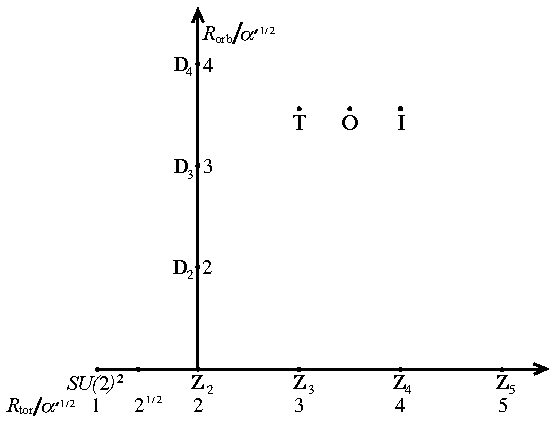
\includegraphics[width=0.78\linewidth]{figures/fig_8_2.pdf}
\caption{$c=1$ の CFT のモジュライ空間。トーラスの枝は水平方向、オービフォールドの枝は垂直方向に伸びる。$SU(2)$ の離散部分群によるツイストから得られる特別な点を示した。これには、正四面体群、正八面体群、正二十面体群から得られる三つの孤立点も含まれる。$R=(2\alpha')^{1/2}$ のトーラスなど、他の特別な半径は後に現れる。}
\label{fig:8.2}
\end{figure}

トーラスの枝とオービフォールドの枝が交わる点の近くの低エネルギー物理を解析すると理解が深まる。この点を、式 (8.5.20) の $r'$ によって $SU(2)$ 理論をツイストしたものとして記述しよう。ツイスト後に残る質量のないスカラーは、$j^3\widetilde j^3$ と、$i,j\in\{1,2\}$ に対する $j^i\widetilde j^j$ である。これらはすべて非ツイストなので、ポテンシャルはツイスト前と同じ $\det M$ である。スカラー場 $M_{ij}$ は再び $U(1)\times U(1)$ 回転によって対角化でき、ちょうど一つの対角成分だけがゼロでない場合にポテンシャルは平坦になる。しかし今度は、モジュラス $M_{33}$ を $M_{11}$ や $M_{22}$ へ回転できないので、これらの方向は物理的に異なる。モジュラス $M_{33}$ は $U(1)\times U(1)$ を破らず、トーラスの枝に沿う移動に対応する。モジュラス $M_{11}$ または $M_{22}$ はゲージ対称性を破り、オービフォールドの枝に沿う移動に対応する。このモジュラスは荷電しているため、その符号反転はゲージ変換である。したがって、物理的に異なるオービフォールドの線は、二つの枝が交わる点で終わる。二つのモジュラスを同時に変化させることはできない。その線形結合はポテンシャルの平坦方向ではないからである。オービフォールド上の弦理論が円上の弦理論と等価になりうるのは非常に驚くべきことであり、弦が時空幾何をわれわれと同じようには見ていないことを、さらに示している。

トーラスの枝に沿って進むと、$SU(2)$ 半径のすべての整数倍 $R=k\alpha'^{1/2}$ に、余分な質量のない状態がある。これらは $(n,w)=(\pm2k,0)$ の状態である。T 双対な記述 $R=\alpha'^{1/2}/k$ において、これらの点は $SU(2)\times SU(2)$ 理論を $\mathbb Z_k$ 対称性
\begin{equation}
X^{25}\longrightarrow X^{25}+\frac{2\pi\alpha'^{1/2}}{k}
\tag{8.5.22}\label{eq:8.5.22}
\end{equation}
でツイストして得られると考えられる。これは $j^1+ij^2$ と $\widetilde j^1+i\widetilde j^2$ に $\exp(2\pi i/k)$ を掛けるので、残る質量のないスカラーは
\begin{equation}
j^3\widetilde j^3,\qquad
j^1\widetilde j^1+j^2\widetilde j^2,\qquad
j^1\widetilde j^2-j^2\widetilde j^1
\tag{8.5.23}\label{eq:8.5.23}
\end{equation}
である。第一のものはトーラスの半径を変えるので、いつものように平坦方向である。しかし、これらの点から別の枝が伸びることはない。$M_{11}=M_{22}$ または $M_{12}=-M_{21}$ の方向では、ポテンシャルが平坦方向をもつための条件 (8.3.23) が満たされないからである。

シフト (8.5.22) は $SU(2)\times SU(2)$ の部分群 $\mathbb Z_k$ を生成する。他の部分群によるツイストを考えよう。シフト (8.5.22) と反射 $X^{25}\to-X^{25}$ が生成する二面体群 $\mathbb D_k$ は、半径 $k\alpha'^{1/2}$ のオービフォールドを与える。他の三つの離散部分群は、正四面体群、正八面体群、正二十面体群である。これらは CFT のモジュライを\textbf{すべて}取り除くので、ツイスト後の CFT は連続な族の一員ではなく、孤立点になる。すべての半径で定義できる $\mathbb Z_k$ および $\mathbb D_k$ ツイストと異なり、これらの離散群は臨界半径にしか存在しない $SU(2)$ の元を含むので、ツイスト後に半径を変えられない。このようなコンパクト空間をもつ弦理論には、スカラーはディラトン一つしかない。以上が知られている $c=1$ の CFT のすべてであり、したがって、知られている25次元のボソン弦背景のすべてを与える。

\subsectionlink{開弦}\label{sec:8.6}

開弦のトーラスコンパクト化に新たに現れるのは、ゲージ場の平坦な背景である、非自明な \textbf{Wilson 線}が可能になることである。まず、いくつかの荷電場を含む $U(1)$ ゲージ理論を調べ、定数背景
\begin{equation}
A_{25}(x^M)=-\frac{\theta}{2\pi R}
=-i\Lambda^{-1}\frac{\partial\Lambda}{\partial x^{25}},
\qquad
\Lambda(x^{25})=\exp\left(-\frac{i\theta x^{25}}{2\pi R}\right)
\tag{8.6.1}\label{eq:8.6.1}
\end{equation}
を考えよう。ここで $\theta$ は定数である。局所的には、これは純粋ゲージである。場の強さはゼロで、場の方程式は自明に満たされる。しかしゲージパラメーター $\Lambda$ は時空の周期性を満たさず、この背景は物理的効果をもつ。それを測るゲージ不変量が Wilson 線
\begin{equation}
W_q=\exp\left(iq\oint dx^{25}\,A_{25}\right)
=\exp(-iq\theta)
\tag{8.6.2}\label{eq:8.6.2}
\end{equation}
である。

まず電荷 $q$ の点粒子を考える。そのゲージ固定した世界線作用は
\begin{equation}
S=\int d\tau\left(\frac12\dot X^M\dot X_M
+\frac{m^2}{2}-iqA_M\dot X^M\right)
\tag{8.6.3}\label{eq:8.6.3}
\end{equation}
である。ゲージ場との作用は単に $-iq\int dx^M A_M$ なので、コンパクト方向を一周する経路は、Wilson 線 $W_q$ に等しい位相を得る。正準運動量は
\begin{equation}
p_{25}=-\frac{\partial L}{\partial v^{25}}
=v^{25}-\frac{q\theta}{2\pi R}
\tag{8.6.4}\label{eq:8.6.4}
\end{equation}
であり、式 (8.4.6) と同様に $v^{25}=i\dot X^{25}$ である。波動関数はコンパクト空間で周期的でなければならないので、整数 $l$ に対して $p_{25}=l/R$ となり、
\begin{equation}
v_{25}=\frac{2\pi l+q\theta}{2\pi R}
\tag{8.6.5}\label{eq:8.6.5}
\end{equation}
を得る。物理的状態を消す Hamiltonian は
\begin{equation}
H=\frac12\left(p_\mu p^\mu+v_{25}^2+m^2\right)
\tag{8.6.6}\label{eq:8.6.6}
\end{equation}
なので、$v_{25}$ が $\theta$ に依存することにより、質量 $-p_\mu p^\mu$ はずれる。同じスペクトルは、粒子ではなく場による記述でも容易に得られる。$v_{25}$ はまさにゲージ不変な運動量 $-i\partial_{25}-qA_{25}$ であることに注意しよう。

ゲージ変換 $\Lambda^{-1}$ によって $A_{25}$ をゼロにしてもよい。このゲージでは、荷電場はもはや周期的でなく、$x^{25}\to x^{25}+2\pi R$ のもとで位相 $\exp(iq\theta)$ を得る。物理的な、すなわちゲージ不変な量は依然として周期的である。今度は正準運動量がずれて、
\begin{equation}
v_{25}=p_{25}=\frac{2\pi l+q\theta}{2\pi R}
\tag{8.6.7}\label{eq:8.6.7}
\end{equation}
となり、ゲージ不変な運動量 $v_{25}$ については先ほどと同じ結果になる。

次に弦に移り、$U(n)$ の Chan--Paton 因子を含めよう。一般の定数 $A_{25}$ はゲージ変換で対角化でき、
\begin{equation}
A_{25}=-\frac1{2\pi R}\operatorname{diag}(\theta_1,\theta_2,\ldots,\theta_n)
\tag{8.6.8}\label{eq:8.6.8}
\end{equation}
となる。ゲージ場は $U(n)$ の対角部分群、すなわち $U(1)^n$ に属する。ゲージ場は一般の状態の Chan--Paton 因子に $[A_M,\lambda]$ として結合するので、Chan--Paton 状態 $|ij\rangle$ にある弦は、$U(1)_i$ のもとで電荷 $+1$、$U(1)_j$ のもとで電荷 $-1$ をもち、他の因子に対しては中性である。したがって、
\begin{equation}
v_{25}=\frac{2\pi l-\theta_j+\theta_i}{2\pi R}
\tag{8.6.9}\label{eq:8.6.9}
\end{equation}
となる。開弦のスペクトルは
\begin{equation}
m^2=\frac{(2\pi l-\theta_j+\theta_i)^2}{4\pi^2R^2}
+\frac1{\alpha'}(N-1)
\tag{8.6.10}\label{eq:8.6.10}
\end{equation}
である。

特にゲージボソンを考えると、$l=0$、$N=1$ なので、
\begin{equation}
m^2=\frac{(\theta_j-\theta_i)^2}{4\pi^2R^2}
\tag{8.6.11}\label{eq:8.6.11}
\end{equation}
となる。一般の背景では、すべての $\theta$ が異なり、質量のないベクトルは $i=j$ の対角成分だけである。この場合、破れていないゲージ群は $U(1)^n$ である。$r$ 個の $\theta$ が等しければ、対応する $r\times r$ 行列のベクトルが質量を失い、$U(r)$ ゲージ対称性を担う。$n$ 個の $\theta$ が、それぞれ $r_i$ 個ずつ等しい組に分かれるとき、ゲージ対称性は
\begin{equation}
U(r_1)\times\cdots\times U(r_s),\qquad
\sum_{i=1}^{s}r_i=n
\tag{8.6.12}\label{eq:8.6.12}
\end{equation}
となる。

いつものように、低エネルギーでの解釈がある。ゲージ場 $A_{25}$ は $U(n)$ の随伴表現に属する25次元スカラーであり、その真空期待値が対称性を自発的に $U(r_1)\times\cdots\times U(r_s)$ へ破る。低エネルギー有効作用の詳細は読者に委ねる。重要なのは、コンパクト方向が $k$ 個あるとき、ポテンシャルに、26次元 Yang--Mills 作用の場の強さから来る項
\begin{equation}
\operatorname{Tr}\left([A_m,A_n]^2\right)
\tag{8.6.13}\label{eq:8.6.13}
\end{equation}
が含まれることである。このため、静的解では異なる方向のゲージ場は可換でなければならず、同時に対角化できる。したがって、ゲージ場から $kn$ 個、計量と反対称テンソルから $k^2$ 個のモジュライが得られる。

\subsubsectionlink*{T 双対性}

開弦スペクトルの $R\to0$ 極限を考えよう。Neumann 境界条件をもつ開弦には、$w$ に相当する量子数がない。周期方向の巻き付きを常にほどけるからである。したがって $R\to0$ では、運動量がゼロでない状態の質量は無限大になるが、新たな連続状態は現れない。振る舞いは場の理論と同じで、残る状態は25次元時空を運動する。

開弦を含む理論には必ず閉弦もあることを思い出すと、一見したところ逆説が生じる。$R\to0$ 極限で閉弦は26次元時空を運動するのに、開弦は25次元しか運動しないからである。何が起きているかは、次のように考えられる。開弦の内部は閉弦と同じ「物質」からできているので、依然として26次元で振動しているはずである。開弦を特徴付けるものは端点なので、25次元の超平面に制限されなければならないのは、この端点である。

\begin{figure}[tbp]
\centering
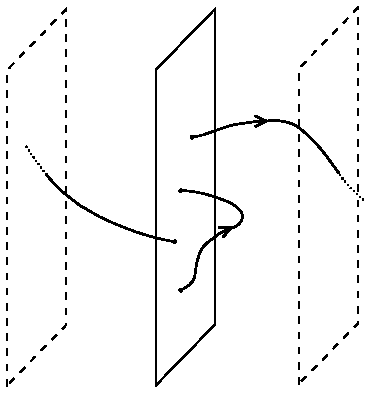
\includegraphics[width=0.62\linewidth]{figures/fig_8_3.pdf}
\caption{端点が超平面に付いた開弦。破線の平面は周期的に同一視されている。巻き付き数が0と1の二本の弦を示す。}
\label{fig:8.3}
\end{figure}

実際、T 双対理論を、新しい埋め込み座標
\begin{equation}
X'^{25}(z,\bar z)=X_L^{25}(z)-X_R^{25}(\bar z)
\tag{8.6.14}\label{eq:8.6.14}
\end{equation}
を使って記述することを思い出そう。このとき
\begin{equation}
\partial_nX^{25}=-i\partial_tX'^{25}
\tag{8.6.15}\label{eq:8.6.15}
\end{equation}
であり、$n$ は境界に垂直、$t$ は境界に接する方向を表す。元の座標に対する Neumann 条件は、双対座標に対する Dirichlet 条件である。すなわち、弦の各端点の $X'^{25}$ 座標が固定される。

まず Wilson 線のないコンパクト化を考えよう。この場合、実はすべての端点が\textbf{同じ}超平面上に拘束される。これを見るために、次を積分する。
\begin{equation}
\begin{split}
X'^{25}(\pi)-X'^{25}(0)
&=\int_0^\pi d\sigma^1\,\partial_1X'^{25}
=-i\int_0^\pi d\sigma^1\,\partial_2X^{25}\\
&=-2\pi\alpha'v^{25}
=-\frac{2\pi\alpha'l}{R}=-2\pi lR'.
\end{split}
\tag{8.6.16}\label{eq:8.6.16}
\end{equation}
両端の間での $X'^{25}$ の変化は、双対方向の周期 $2\pi R'$ の整数倍なので、周期的な T 双対空間では両端は同じ超平面にある。二本の\textbf{異なる}開弦については、それらの間の重力子交換によって得られる連結な世界面を考えよう。任意の二つの端点を結ぶ経路に沿って、同じ議論 (8.6.16) を適用できる。したがって図8.3のように、すべての弦のすべての端点は同じ超平面上にある。他の24個の空間方向では、端点は依然として自由に動ける。

\begin{figure}[tbp]
\centering
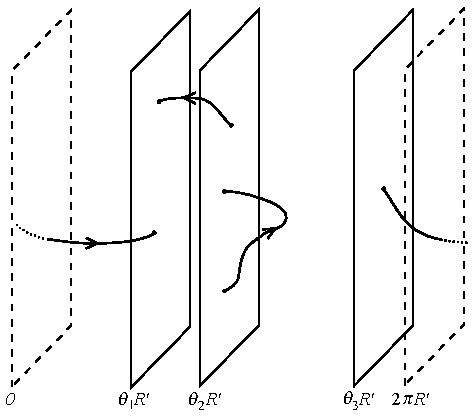
\includegraphics[width=0.72\linewidth]{figures/fig_8_4.pdf}
\caption{異なる位置にある $n=3$ 枚の超平面と、それらに付いたさまざまな弦。タキオンを無視すると、両端が同じ超平面上にある最も軽い弦は質量がない。一方、一致しない超平面間に張られた弦は、その張力のために質量をもつ。二つの超平面が一致すると、それらの間に張られた最も軽い弦は質量を失う。}
\label{fig:8.4}
\end{figure}

次に Wilson 線の効果を考える。$v_{25}$ のシフト (8.6.9) によって、差 (8.6.16) は
\begin{equation}
\Delta X'^{25}=X'^{25}(\pi)-X'^{25}(0)
=-(2\pi l-\theta_j+\theta_i)R'
\tag{8.6.17}\label{eq:8.6.17}
\end{equation}
に置き換わる。言い換えると、任意の加法定数を除いて、状態 $i$ の端点の位置は
\begin{equation}
X'^{25}=\theta_iR'=-2\pi\alpha'A_{25,ii}
\tag{8.6.18}\label{eq:8.6.18}
\end{equation}
である。したがって一般に、図8.4に示すように、異なる位置に $n$ 枚の超平面がある。

Chan--Paton 状態 $|ij\rangle$ をもち、コンパクト方向に $l$ 回巻き付く開弦のセクターでのモード展開は、
\begin{equation}
\begin{split}
X'^{25}(z,\bar z)
={}&\theta_iR'-\frac{iR'}{2\pi}(2\pi l-\theta_j+\theta_i)\ln(z/\bar z)\\
&+i\left(\frac{\alpha'}2\right)^{1/2}
\sum_{\substack{m=-\infty\\m\ne0}}^\infty
\frac{\alpha_m^{25}}{m}(z^{-m}-\bar z^{-m})\\
={}&\theta_iR'+\frac{\sigma^1}{\pi}\Delta X'^{25}
-(2\alpha')^{1/2}
\sum_{\substack{m=-\infty\\m\ne0}}^\infty
\frac{\alpha_m^{25}}{m}\exp(-m\sigma^2)\sin m\sigma^1.
\end{split}
\tag{8.6.19}\label{eq:8.6.19}
\end{equation}
スペクトル (8.6.10) は
\begin{equation}
m^2=\left(\frac{\Delta X'^{25}}{2\pi\alpha'}\right)^2
+\frac1{\alpha'}(N-1)
\tag{8.6.20}\label{eq:8.6.20}
\end{equation}
となる。ここで式 (8.6.17) で与えられる $\Delta X'^{25}$ は、与えられたセクターの弦の最小長さである。

例えば $p+1\leq m\leq25$ に対する $X^m$ のように、複数の座標が周期的であり、それらの方向を双対座標で書き直す場合に、この描像がどのように一般化されるかを考えよう。$X^m$ の Neumann 条件は再び双対座標 $X'^m$ の Dirichlet 条件になるので、開弦の端点は、平行な $n$ 個の $(p+1)$ 次元部分空間に閉じ込められる。各方向の Wilson 線は、各部分空間の独立な座標となる。

双対な描像は、開弦の境界条件によって並進不変性が破れているという点で、いささか奇妙である。これは単に、元の開弦理論では巻き付き数が保存されないことを反映している。巻き付いた閉弦は切れて開き、巻き付きをほどける。そして巻き付き数は、T 双対性によって運動量に対応する。T 双対性は同じ理論の異なる記述にすぎず、さらに、元の理論のコンパクト化半径が小さいときには、T 双対な描像を使うのが自然であることを覚えておく必要がある。この場合、図8.4が、得られる物理をどのように解釈すればよいかを示している。

\subsectionlink{D ブレーン}\label{sec:8.7}

開弦理論を小さなトーラス上にコンパクト化すると、その物理は、大きなトーラスへのコンパクト化において、開弦の端点を部分空間上に制限したものとして記述されることがわかった。実は、これらの部分空間は、それ自体が新しい力学的な対象である。簡単のため、双対化する座標が一つだけの場合を取り、すべての $\theta_i$ が異なる一般の配置における、質量のない開弦のスペクトルを考えよう。タキオンを無視すると、質量 (8.6.20) がゼロになるのは $N=1$、$\Delta X'^{25}=0$ の場合だけである。すなわち、両端は同じ超平面上にあり、巻き付き数はゼロである。したがって、質量のない状態
\begin{align}
&\alpha_{-1}^\mu|k;ii\rangle,\qquad
\mathcal V=i\partial_tX^\mu,
\tag{8.7.1a}\label{eq:8.7.1a}\\
&\alpha_{-1}^{25}|k;ii\rangle,\qquad
\mathcal V=i\partial_tX^{25}=\partial_nX'^{25}
\tag{8.7.1b}\label{eq:8.7.1b}
\end{align}
が得られる。

もちろん、これらは元の理論と同じ質量のない状態であり、T 双対性は同じスペクトルに別の描像を与えるだけである。一般の Wilson 線の場合、元の理論における質量のない開弦状態は、$n$ 個の質量のない $U(1)$ ベクトルだけだった。式 (8.7.1) では、それらを偏極が超平面に接するか、垂直かによって分けた。接する偏極をもつ25個の状態は、超平面上に存在するゲージ場をなす。垂直な偏極をもつ状態は、元の理論ではコンパクト方向のゲージ場であったが、T 双対理論では単純かつ重要な解釈をもつ。それは超平面の形状に対する\textbf{集団座標}である。定数のゲージ背景 (8.6.18) が超平面の一様な並進に対応することから、これはすでに明らかである。同じ理由で、$x^\mu$ に依存する背景は $x^\mu$ に依存する並進、すなわち曲がった超平面へ移り、場 $A_{ii}^{25}$ の量子は、超平面の小さな振動に対応する。

これは時空そのものに起きたのと同じ現象である。平坦な背景における弦から始めて、ある質量のない閉弦状態が幾何の揺らぎに対応すると発見した。ここでは、まず超平面が現れ、次に、ある開弦状態がその形状の揺らぎに対応するとわかった。超平面が力学的になったことは、驚くべきではない。弦理論は重力を含む。超平面を通過する重力波は時空そのものを歪めるので、超平面だけが剛体のままでいるとは考えにくい。

したがって、この超平面は確かに力学的な対象であり、\textbf{Dirichlet 膜}、略して\textbf{D ブレーン}である。$25-p$ 個の方向を双対化して得られる $p$ 次元 D ブレーンを D$p$ ブレーンと呼ぶ。この用語では、元の $U(n)$ 開弦理論には $n$ 枚の D25 ブレーンが含まれる。D25 ブレーンは空間を満たすので、弦の端点はどこにあってもよい。これは通常の Chan--Paton 因子に対応するだけである。

T 双対性は Neumann 境界条件と Dirichlet 境界条件を入れ替えるので、D$p$ ブレーンに接する方向でさらに T 双対変換すると、D$(p-1)$ ブレーンになる。一方、垂直な方向の T 双対変換では D$(p+1)$ ブレーンになる。自明でない角度をなす場合は、まもなく現れる。

Dirichlet 境界条件を、それ自体として調べるところから始めることもできた。ここで採った、T 双対性を通してそれを発見する道筋は、その多くの性質を導くのに適している。またこれは、「通常の」状態から連続的な過程によって、D ブレーンを含む状態に到達できることも示している。すなわち、元の理論の $R\to0$ 極限を取れば、非コンパクト空間に D ブレーンが残る。超弦では、このことを用いて、D ブレーンが理論の非摂動的定義に不可欠な要素であると論じる。ボソン弦については、この議論を試みない。理論が非摂動的な定義をもつという強い根拠がないからである。ボソン弦理論は、超弦理論の一部を切り落としたものとしてしか存在しないのかもしれない。

$U(n)$ の対称性の破れを、T 双対な描像で見るのは興味深い。どの D ブレーンも一致していないとき、各ブレーンには質量のないベクトルが一つだけあり、全体のゲージ群は $U(1)^n$ となる。$r$ 枚の D ブレーンが一致すると、それらの間に張られた弦の長さがゼロになれるため、新たな質量のない状態が現れる。質量公式 (8.6.20) の $\Delta X'^{25}$ は、$i,j$ の両方がこの $r$ 枚の集合に属していれば、$n=0$ でゼロになる。したがって、$U(r)$ ゲージ群の随伴表現をなす $r^2$ 個のベクトルがある。これは双対な Wilson 線の描像で見いだしたものと同じである。しかし注目すべきことに、D ブレーンに垂直な成分から、質量のないスカラーも $r^2$ 個現れる。この意味は以下で論じる。

\subsubsectionlink*{D ブレーン作用}

D$p$ ブレーンの世界体積上の質量のない場は、$U(1)$ ベクトルと、揺らぎを記述する $25-p$ 個の世界ブレーン上のスカラーである。この系の低エネルギー有効作用を考えることは、いつものように非常に有用である。ここで双対半径 $R'$ を無限大にし、得られる26次元時空の中の一枚の D ブレーンに注目する。世界ブレーン上の場は、第3.7節ですでに作用を論じた、質量のない閉弦場と相互作用している。ブレーン上に座標 $\xi^a$、$a=0,\ldots,p$ を導入する。ブレーン上の場は埋め込み $X^\mu(\xi)$ とゲージ場 $A_a(\xi)$ である。作用は
\begin{equation}
\boldsymbol S_p=-T_p\int d^{p+1}\xi\,e^{-\Phi}
\left[-\det(G_{ab}+B_{ab}+2\pi\alpha'F_{ab})\right]^{1/2}
\tag{8.7.2}\label{eq:8.7.2}
\end{equation}
であると主張する。$T_p$ は後で決定する定数である。ここで、
\begin{equation}
\begin{split}
G_{ab}(\xi)&=\frac{\partial X^\mu}{\partial\xi^a}
\frac{\partial X^\nu}{\partial\xi^b}G_{\mu\nu}(X(\xi)),\\
B_{ab}(\xi)&=\frac{\partial X^\mu}{\partial\xi^a}
\frac{\partial X^\nu}{\partial\xi^b}B_{\mu\nu}(X(\xi))
\end{split}
\tag{8.7.3}\label{eq:8.7.3}
\end{equation}
は、ブレーン上の誘導計量と誘導反対称テンソルである。

作用 (8.7.2) の特徴はすべて、一般的な考察から理解できる。まず時空計量と埋め込みだけを考えると、最も単純で微分の次数が最も低い、座標不変な作用は、世界体積 $(-\det G_{ab})^{1/2}$ の積分である。これは誘導場 (8.7.3) を通して $X^\mu(\xi)$ に暗黙に依存することに注意しよう。平坦な D ブレーンのまわりで展開すると、Nambu--Goto 作用が弦の揺らぎを記述するのと同様に、揺らぎの作用を与える。

ディラトン依存性 $e^{-\Phi}\propto g_{\mathrm c}^{-1}$ は、これが開弦の木レベル作用であるために現れる。開弦場の自己相互作用も、閉弦場への結合も、まず円板から生じる。

$F_{ab}$ への依存性は T 双対性を用いて理解できる。$X^1$ 方向と $X^2$ 方向に伸びる D ブレーンを考え、他の方向は指定しないことにし、その上に定数のゲージ場 $F_{12}$ があるとする。$A_2=X^1F_{12}$ のゲージに移ろう。次に2方向で T 双対変換する。この方向の Neumann 条件は Dirichlet 条件に置き換わるので、D ブレーンの次元は一つ減る。しかし、ポテンシャルと座標の間の T 双対関係 (8.6.18) から、D ブレーンは $(1\text{--}2)$ 平面内で傾き、
\begin{equation}
X'^2=-2\pi\alpha'X^1F_{12}
\tag{8.7.4}\label{eq:8.7.4}
\end{equation}
となる。この傾きは、作用に幾何学的因子
\begin{equation}
\int dX^1\left[1+(\partial_1X'^2)^2\right]^{1/2}
=\int dX^1\left[1+(2\pi\alpha'F_{12})^2\right]^{1/2}
\tag{8.7.5}\label{eq:8.7.5}
\end{equation}
を与える。

任意の D ブレーンに対して、ブーストで座標軸にそろえ、次に回転で $F_{ab}$ をブロック対角形にすれば、作用を各平面の因子 (8.7.5) の積へ帰着できる。これは行列式 (8.7.2) 中の $F_{ab}$ 項と等価である。この行列式の形をしたゲージ場の作用は Born--Infeld 作用として知られる。当初は、量子電磁力学の短距離発散の解決として提案されたが、その目的では成功しなかった。

最後に、$B_{ab}$ への依存性は次の議論で与えられる。閉弦場 $B_{\mu\nu}$ と開弦場 $A^\mu$ は、弦の世界面作用に次の形で現れる。\footnote[3]{微分形式に詳しい読者のために書くと、これは
\[
\frac{i}{2\pi\alpha'}\int_M B+i\int_{\partial M}A
\]
である。以下の式も同様に書き直せる。}
\begin{equation}
\frac{i}{4\pi\alpha'}\int_M d^2\sigma\,g^{1/2}
\epsilon^{ab}\partial_aX^\mu\partial_bX^\nu B_{\mu\nu}
+i\int_{\partial M}dX^\mu A_\mu.
\tag{8.7.6}\label{eq:8.7.6}
\end{equation}
これらの場にはそれぞれ時空のゲージ不変性があり、時空理論の整合性のために、それらを保たなければならない。通常のゲージ変換
\begin{equation}
\delta A_\mu=\partial_\mu\lambda
\tag{8.7.7}\label{eq:8.7.7}
\end{equation}
は作用 (8.7.6) の対称性である。境界項の変化が全微分の積分だからである。反対称テンソルの変換
\begin{equation}
\delta B_{\mu\nu}=\partial_\mu\zeta_\nu-\partial_\nu\zeta_\mu
\tag{8.7.8}\label{eq:8.7.8}
\end{equation}
も同様に、バルク作用を全微分だけ変えるが、境界をもつ世界面では、これは表面項を生む。これを打ち消すには、開弦場 $A_\mu$ もテンソルのゲージ対称性のもとで
\begin{equation}
\delta A_\mu=-\frac{\zeta_\mu}{2\pi\alpha'}
\tag{8.7.9}\label{eq:8.7.9}
\end{equation}
と変換しなければならない。しかしこのとき、両方の対称性のもとで不変なのは組合せ
\begin{equation}
B_{\mu\nu}+2\pi\alpha'F_{\mu\nu}
\equiv2\pi\alpha'\mathcal F_{\mu\nu}
\tag{8.7.10}\label{eq:8.7.10}
\end{equation}
だけであり、作用にはこの組合せが現れなければならない。こうして作用の形 (8.7.2) が完全に決まる。

確認として、$G_{\mu\nu}+B_{\mu\nu}$ という組合せが現れるのは自然である。同じ組合せが共形ゲージの世界面作用に現れるからである。なお、作用 (8.7.2) は、さまざまな開弦振幅および開弦と閉弦を含む振幅の低エネルギー極限を取ることによっても求められるが、その方が手間はかかる。

互いに離れた $n$ 枚の D ブレーンについては、作用は単一の D ブレーンの作用を $n$ 個足したものである。しかし、D ブレーンが一致すると、ブレーン上の質量のないベクトルとスカラーは $n$ 個でなく $n^2$ 個になることを見た。これらを支配する有効作用を書きたい。今や場 $X^\mu(\xi)$ と $A_a(\xi)$ は $n\times n$ 行列である。ゲージ場についての意味は明らかで、非 Abel な $U(n)$ ゲージ場になる。しかし集団座標 $X^\mu$ についての意味は謎めいている。時空への $n$ 枚の D ブレーンの埋め込みを表す集団座標が、$n\times n$ 行列へ拡大されているのである。この「非可換幾何」が D ブレーンの力学に重要な役割を果たすことは明らかになっており、時空の本性に関する重要な手がかりであるとの推測もある。

有効作用を考えると、さらに理解が進む。今度は作用に微分を含まない項、すなわち集団座標のポテンシャルがあり、これは定数の $A_m$ 場から T 双対性によって導ける。このようなベクトルポテンシャルでは、場の強さは単に $[A_m,A_n]$ であり、T 双対な描像では $(2\pi\alpha')^{-2}[X_m,X_n]$ になる。場の強さで展開すると、作用の先頭項は概略
\begin{equation}
V\propto\operatorname{Tr}\left([X_m,X_n][X^m,X^n]\right)
\tag{8.7.11}\label{eq:8.7.11}
\end{equation}
となる。このポテンシャルは、点 $X^m=0$ において二階微分がゼロになるので、$kn^2$ 個のスカラーはすべて質量がない。ここでも $k=25-p$ は双対化した方向の数である。しかし平坦方向の空間は、それより小さい。ポテンシャルは二乗の和なので、すべての $[X^m,X^n]$ がゼロである場合に限ってゼロになる。その場合には、$U(n)$ ゲージ対称性を使って、すべての $X^m$ が対角となるゲージへ移れる。したがって平坦方向は、対角成分の個数に等しい $kn$ 個である。これら $kn$ 個の対角成分は、$n$ 枚の D$p$ ブレーンの集団座標と解釈できる。ゆえにポテンシャル (8.7.11) は、離れた D ブレーンと一致した D ブレーンの物理を正しくつなぐ。

$X^m$ が可換な場合、作用は互いに離れた $n$ 枚の D ブレーンの作用に帰着しなければならないので、
\begin{equation}
\begin{split}
\boldsymbol S_p=-T_p\int d^{p+1}\xi\,
\operatorname{Tr}\bigl\{&
e^{-\Phi}[-\det(G_{ab}+B_{ab}+2\pi\alpha'F_{ab})]^{1/2}\\
&+O([X^m,X^n]^2)\bigr\}
\end{split}
\tag{8.7.12}\label{eq:8.7.12}
\end{equation}
でなければならない。行列式は世界体積の添字 $ab$ に関して取り、トレースは $n$ 個の Chan--Paton 添字に関して取る。このトレースは適切な $U(n)$ 不変量であり、対角行列の場合には個々の D ブレーンについての和に帰着する。交換子への完全な依存性は、単純なポテンシャル (8.7.11) より複雑で、他の場への追加の結合や、交換子の高次の補正がある。しかし重要な性質、すなわち平坦方向の形は変わらない。完全な依存性は、すべての方向が Neumann 条件を満たす場合の Born--Infeld 作用から出発して、T 双対変換を行うことで求められる。なお、場の強さの交換子を含む高階微分項は、T 双対性だけでは決定できない。

\subsubsectionlink*{D ブレーンの張力}

定数 $T_p$ を計算することは理解を深めるうえで有用であり、超弦ではその正確な値が重要になる。具体的な計算を行う前に、T 双対性から $T_p$ の漸化式が得られることに注目しよう。ディラトンが定数の背景では、D$p$ ブレーンの張力は $T_pe^{-\Phi}$ である。これは静的な D ブレーンの単位体積あたりの作用に負号を付けたものだからである。ここで D$p$ ブレーンに接する $p$ 個の方向が周期的に同一視されている場合を考えよう。すなわち、D$p$ ブレーンは時空内の $p$ 次元トーラスに\textbf{巻き付いている}。その質量は張力とトーラスの体積の積
\begin{equation}
T_pe^{-\Phi}\prod_{i=1}^{p}(2\pi R_i)
\tag{8.7.13}\label{eq:8.7.13}
\end{equation}
である。周期方向の一つ $X^p$ で T 双対変換しよう。これは同じ状態の新しい記述にすぎないので、質量を変えない。T 双対理論のディラトン (8.3.31) を用いると、質量 (8.7.13) は
\begin{equation}
2\pi\alpha'^{1/2}T_pe^{-\Phi'}
\prod_{i=1}^{p-1}(2\pi R_i)
\tag{8.7.14}\label{eq:8.7.14}
\end{equation}
となる。しかし双対理論では、これは $(p-1)$ 次元トーラスに巻き付いた D$(p-1)$ ブレーンなので、その質量は
\begin{equation}
T_{p-1}e^{-\Phi'}\prod_{i=1}^{p-1}(2\pi R_i)
\tag{8.7.15}\label{eq:8.7.15}
\end{equation}
である。質量 (8.7.14) と (8.7.15) を等置すると、
\begin{equation}
T_p=\frac{T_{p-1}}{2\pi\alpha'^{1/2}}
\tag{8.7.16}\label{eq:8.7.16}
\end{equation}
を得る。これによって、全体の規格化定数一つを除いて $T_p$ が決まる。

\begin{figure}[tbp]
\centering
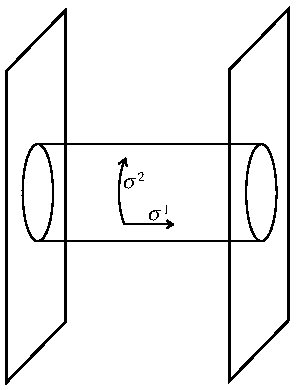
\includegraphics[width=0.64\linewidth]{figures/fig_8_5.pdf}
\caption{二枚の D ブレーン間の閉弦交換。等価に、各 D ブレーンに片端ずつ付いた開弦の真空ループである。}
\label{fig:8.5}
\end{figure}

D ブレーンの張力の実際の値を決めるには、弦振幅を計算する必要がある。例えば、重力子の頂点演算子をもつ円板で与えられる、D ブレーンへの重力結合から求めてもよい。しかし、そこにはまだわかっていない比 $g_{\mathrm c}/g_{\mathrm o}^2$ が含まれる。閉弦結合は頂点演算子から、開弦結合は円板から現れる。代わりに、次のように絶対的な規格化を求められる。位置 $X_1^m=0$ と $X_2^m=y^m$ にある、平行な二枚の D$p$ ブレーンを考えよう。この二つの対象は、図8.5のように閉弦を交換することで互いの存在を感じる。この弦振幅は頂点演算子をもたないアニュラスなので、前章と同じ方法で計算できる。重力子とディラトンの交換による極から、閉弦状態の D ブレーンへの結合 $T_p$ が得られる。

第7.4節では、アニュラスの真空振幅を開弦のループとして計算したが、モジュライ積分の $t\to0$ 極限から閉弦の極が見つかったことを思い出そう。ここで関心があるのはまさにそれらの極だが、振幅を計算する最も簡単な方法は、やはり開弦のループとみなすことである。実際、先の結果 (7.4.1) は、わずかな変更だけで適用できる。運動量積分の数は26から $p+1$ へ減り、それに応じて $V_{26}$ は $V_{p+1}$ になる。ウェイト $h_i$ には、伸びた弦の張力から $y^2/(4\pi^2\alpha')$ が加わる。Chan--Paton のウェイト $n^2$ は2になる。弦はどちらの向きにも付けられるからである。したがって、
\begin{equation}
\begin{split}
\mathcal A
&=iV_{p+1}\int_0^\infty\frac{dt}{t}
(8\pi^2\alpha't)^{-(p+1)/2}
\exp(-ty^2/2\pi\alpha')\eta(it)^{-24}\\
&=\frac{iV_{p+1}}{(8\pi^2\alpha')^{(p+1)/2}}
\int_0^\infty dt\,t^{(21-p)/2}\exp(-ty^2/2\pi\alpha')\\
&\qquad\times\left[\exp(2\pi/t)+24+\cdots\right]
\end{split}
\tag{8.7.17}\label{eq:8.7.17}
\end{equation}
を得る。漸近形は、第7.4節とまったく同様にして求めた。第一項はタキオン交換から来るので、やはりボソン弦特有の、ここでは関心のない効果である。第二項を積分すると、
\begin{equation}
\begin{split}
\mathcal A
&=iV_{p+1}\frac{24}{2^{12}}(4\pi^2\alpha')^{11-p}
\pi^{(p-23)/2}\Gamma\left(\frac{23-p}{2}\right)|y|^{p-23}\\
&=iV_{p+1}\frac{24\pi}{2^{10}}(4\pi^2\alpha')^{11-p}G_{25-p}(y)
\end{split}
\tag{8.7.18}\label{eq:8.7.18}
\end{equation}
を得る。$G_d(y)$ は $d$ 次元の質量のないスカラーの Green 関数、すなわち $-\nabla^2$ の逆である。

次に、これを同じ振幅の場の理論による計算と比較する必要がある。反対称テンソルは D ブレーンに結合しないので、時空作用 (3.7.25) の関係する項は
\begin{equation}
\boldsymbol S=\frac1{2\kappa^2}\int d^{26}X\,(-\widetilde G)^{1/2}
\left(\widetilde{\boldsymbol R}
-\frac16\widetilde\nabla_\mu\widetilde\Phi\,
\widetilde\nabla^\mu\widetilde\Phi\right)
\tag{8.7.19}\label{eq:8.7.19}
\end{equation}
である。チルダは Einstein 計量を表すことを思い出そう。この形は、その作用がディラトンの作用から分離するため便利である。チルダの付いたディラトンは、期待値がゼロになるようシフトしてある。同じ変数を使うと、D ブレーン作用 (8.7.2) の関係する項は
\begin{equation}
\boldsymbol S_p=-\tau_p\int d^{p+1}\xi\,
\exp\left(\frac{p-11}{12}\widetilde\Phi\right)
(-\det\widetilde G_{ab})^{1/2}
\tag{8.7.20}\label{eq:8.7.20}
\end{equation}
となる。$\tau_p=T_pe^{-\Phi_0}$ と定義した。これは、ディラトンの背景値が $\Phi_0$ のときの D$p$ ブレーンの実際の物理的張力である。

図8.5に対応する場の理論のグラフは、D ブレーン間の一個の重力子またはディラトンの交換である。伝播関数を求めるために、時空作用を $h_{\mu\nu}=\widetilde G_{\mu\nu}-\eta_{\mu\nu}$ の二次まで、また $\widetilde\Phi$ の二次まで展開する。重力の計算では、ゲージも選ばなければならない。摂動計算に最も簡単なゲージは
\begin{equation}
F_\nu\equiv\partial^{\widehat\mu}h_{\mu\nu}
-\frac12\partial_\nu h^{\widehat\mu}{}_\mu=0
\tag{8.7.21}\label{eq:8.7.21}
\end{equation}
である。ハットは、平坦時空の計量 $\eta^{\mu\nu}$ によって添字を上げたことを表す。作用を二次まで展開し、ゲージ固定項 $-F_\nu F^{\widehat\nu}/(4\kappa^2)$ を加えると、時空作用は
\begin{equation}
\boldsymbol S=-\frac1{8\kappa^2}\int d^{26}X
\left(
\partial_\mu h_{\nu\lambda}\partial^{\widehat\mu}h^{\widehat\nu\widehat\lambda}
-\frac12\partial_\mu h^{\widehat\nu}{}_\nu
\partial^{\widehat\mu}h^{\widehat\lambda}{}_\lambda
+\frac23\partial_\mu\widetilde\Phi\,
\partial^{\widehat\mu}\widetilde\Phi
\right)
\tag{8.7.22}\label{eq:8.7.22}
\end{equation}
となる。運動項を反転すると、運動量空間の伝播関数
\begin{align}
\langle\widetilde\Phi\widetilde\Phi\rangle
&=-\frac{(D-2)i\kappa^2}{4k^2},
\tag{8.7.23a}\label{eq:8.7.23a}\\
\langle h_{\mu\nu}h_{\sigma\rho}\rangle
&=-\frac{2i\kappa^2}{k^2}
\left(\eta_{\mu\sigma}\eta_{\nu\rho}
+\eta_{\mu\rho}\eta_{\nu\sigma}
-\frac2{D-2}\eta_{\mu\nu}\eta_{\sigma\rho}\right)
\tag{8.7.23b}\label{eq:8.7.23b}
\end{align}
を得る。後で参照するため、一般の $D$ に対する形を示した。平坦な配置のまわりで展開した D ブレーン作用は
\begin{equation}
\boldsymbol S_p=-\tau_p\int d^{p+1}\xi
\left(\frac{p-11}{12}\widetilde\Phi-\frac12h_{aa}\right)
\tag{8.7.24}\label{eq:8.7.24}
\end{equation}
である。ここで $h_{\mu\nu}$ のトレースは、D ブレーンに接する方向だけについて取っていることに注意しよう。$\xi$ は、計量 $\delta_{ab}$ をもつ直交直線座標に取った。

これで Feynman グラフを読み取れる。
\begin{equation}
\begin{split}
\mathcal A
&=\frac{i\kappa^2\tau_p^2}{k_\perp^2}V_{p+1}
\left\{6\left[\frac{p-11}{12}\right]^2
+\frac12\left[2(p+1)-\frac1{12}(p+1)^2\right]\right\}\\
&=\frac{6i\kappa^2\tau_p^2}{k_\perp^2}V_{p+1}.
\end{split}
\tag{8.7.25}\label{eq:8.7.25}
\end{equation}
弦の結果 (8.7.18) と比較すると、
\begin{equation}
\tau_p^2=\frac{\pi}{256\kappa^2}(4\pi^2\alpha')^{11-p}
\tag{8.7.26}\label{eq:8.7.26}
\end{equation}
が得られる。計算を整理した結果が T 双対性からの漸化式を満たすことは、有用な確認となる。

一つの応用として、$n$ 枚の25ブレーンをもつ状態を考えよう。これは、通常の、すべての方向が Neumann 条件を満たす $n$ 値の Chan--Paton 因子と同じである。25ブレーン作用 (8.7.12) をゲージ場の二次まで展開すると、
\begin{equation}
\frac{\tau_{25}}4(2\pi\alpha')^2
\operatorname{Tr}(F_{\mu\nu}F^{\mu\nu})
\tag{8.7.27}\label{eq:8.7.27}
\end{equation}
を得る。これは開弦のゲージ結合と重力結合を関係付ける。式 (6.5.14)、(6.5.16)、(6.6.15)、(6.6.18) を用いれば、頂点演算子の規格化 $g_{\mathrm c}$ と $g_{\mathrm o}$ の関係として、
\begin{equation}
\frac{g_{\mathrm o}^2}{g_{\mathrm c}}
=\frac{4\pi\alpha'g_{\mathrm o}'{}^2}{\kappa}
=2^{18}\pi^{25/2}\alpha'^6
\tag{8.7.28}\label{eq:8.7.28}
\end{equation}
と書ける。これは、開弦結合の二乗が閉弦結合に比例するという正しい形をもち、今度は数値係数も含まれている。本質的には、アニュラス図の閉弦の極で因数分解することによって、ユニタリティからこの結果を得た。演習7.9のように、D ブレーンを経由せず、より直接に求めることもできた。

\subsectionlink{向きのない理論の T 双対性}\label{sec:8.8}

向きのない弦理論の $R\to0$ 極限も、興味深い新しい物理をもたらす。まず閉弦を考えよう。向きのない理論を作るには、状態に $\Omega=+1$ を課す。第8.5節の議論に従えば、これは $\Omega$ のゲージ化と考えられる。特に、世界面を組み立てる際の遷移関数には、今や向きの反転を含めてよい。これはゲージ対称性だからであり、こうして向きのない世界面が生まれる。

T 双対理論は、$X^m(z,\bar z)=X_L^m(z)+X_R^m(\bar z)$ の代わりに、座標 $X'^m(z,\bar z)=X_L^m(z)-X_R^m(\bar z)$ を用いることで得られる。元の記述では、世界面パリティ $\Omega$ をゲージ化しており、その作用は
\begin{equation}
\Omega:\quad X_L^M(z)\longleftrightarrow X_R^M(z)
\tag{8.8.1}\label{eq:8.8.1}
\end{equation}
である。T 双対座標で表すと、これは
\begin{align}
\Omega:\quad X'^m(z,\bar z)&\longleftrightarrow-X'^m(\bar z,z),
\tag{8.8.2a}\label{eq:8.8.2a}\\
X^\mu(z,\bar z)&\longleftrightarrow X^\mu(\bar z,z)
\tag{8.8.2b}\label{eq:8.8.2b}
\end{align}
となる。ここでも $m$ は T 双対化した座標、$\mu$ は双対化していない座標を表す。したがって双対な描像では、対称性 (8.8.2) は世界面パリティ変換と時空反射の積である。世界面パリティだけをゲージ化すると向きのない理論が得られ、反射だけをゲージ化するとオービフォールドが得られることを見た。組み合わせた射影の結果は、\textbf{オリエンティフォールド}として知られる。

オリエンティフォールドは、オービフォールドとよく似ている。弦の波動関数を内部の部分と重心 $x^m$ への依存性に分け、内部の波動関数を $\Omega$ の固有状態に取ろう。すると $\Omega=+1$ への射影により、$-x^m$ での弦の波動関数は、符号を除いて $x^m$ でのものと同じになる。例えば、計量と反対称テンソルの各成分は
\begin{align}
G_{\mu\nu}(x')&=G_{\mu\nu}(x),&
B_{\mu\nu}(x')&=-B_{\mu\nu}(x),
\tag{8.8.3a}\label{eq:8.8.3a}\\
G_{\mu n}(x')&=-G_{\mu n}(x),&
B_{\mu n}(x')&=B_{\mu n}(x),
\tag{8.8.3b}\label{eq:8.8.3b}\\
G_{mn}(x')&=G_{mn}(x),&
B_{mn}(x')&=-B_{mn}(x)
\tag{8.8.3c}\label{eq:8.8.3c}
\end{align}
を満たす。ここで $(x^\mu,x^m)'=(x^\mu,-x^m)$ である。各 $m,n$ に対して負号が付き、さらに各 $B_{MN}$ にもう一つ負号が付く。オービフォールドの場合も同じだが、後者の負号はない。言い換えると、T 双対時空は、オービフォールド構成と同様、トーラス $T^k$ を $k$ 個のコンパクト方向の $\mathbb Z_2$ 反射で同一視したものである。例えば周期方向が一つの場合、双対時空は線分 $0\leq x^{25}\leq\pi R'$ であり、両端にオリエンティフォールド固定平面がある。

\begin{figure}[tbp]
\centering
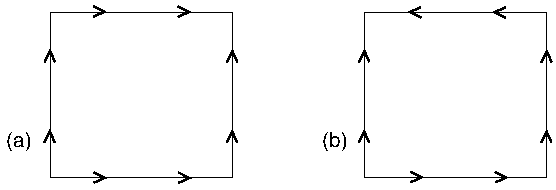
\includegraphics[width=0.78\linewidth]{figures/fig_8_6.pdf}
\caption{(a) トーラスと (b) Klein の壺を定義する同一視。}
\label{fig:8.6}
\end{figure}

また、オリエンティフォールド固定平面から離れた場所では、局所的な物理は\textbf{向きのある}弦理論のものであることにも注意しよう。元の向きのない理論では、射影は局所的に状態の半分を取り除くが、ここでは式 (8.8.3) のように、任意の点での弦の波動関数を、その像の点での値に関係付ける。

オービフォールド構成とオリエンティフォールド構成の相違の一つは、後者にはツイスト状態に直接対応するものがないことである。Klein の壺には、モジュラー変換 $\tau\to-1/\tau$ がないからである。トーラスと Klein の壺を示した図8.6を考えよう。トーラスでは、射影演算子は図8.6(a)の時間方向にツイストを挿入する。図を $90^\circ$ 回転すると、これは空間方向のツイストとなり、スペクトルにツイスト状態が存在することを意味する。しかし図8.6(b)の Klein の壺を $90^\circ$ 回転すると、向かい合う二つの辺で時間の向きが一致せず、このチャネルを中間状態によって解釈することはできない。したがって、オリエンティフォールド平面は力学的になりえないことに注意すべきである。D ブレーンの場合とは異なり、オリエンティフォールド平面に結び付いて、その形状の揺らぎを表す弦のモードはない。重力波が D ブレーンを振動させるという直観的な議論は、オリエンティフォールド平面には適用できない。本質的には、同一視 (8.8.3) が固定平面での境界条件となり、入射波と反射波が打ち消し合う。D ブレーンの場合、反射波は弦結合に関して高次である。

向きのある弦は、その向きを示す矢印を付けて描く。向きのない理論では、矢印を省いてもよいし、二つの向きの線形結合を取ってもよい。後者の描像は離散対称性をゲージ化する考え方とよりよく合致し、また、より一般的である。オリエンティフォールドではパリティ操作に時空変換が伴うので、単に矢印を忘れることはできない。

オリエンティフォールド構成は T 双対性を通して導入したが、トーラスコンパクト化の単なる T 双対ではない、より一般のオリエンティフォールドも考えられる。その場合は、世界面パリティとさまざまな時空対称性を組み合わせた群をゲージ化する。

\begin{figure}[tbp]
\centering
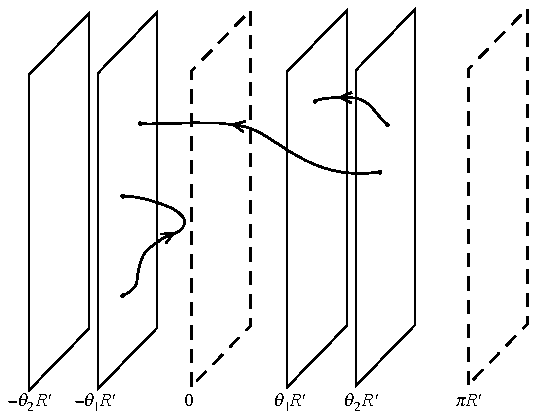
\includegraphics[width=0.78\linewidth]{figures/fig_8_7.pdf}
\caption{$0$ と $\pi R'$ にあるオリエンティフォールド平面、$\theta_1R'$ と $\theta_2R'$ にある D ブレーン、および $-\theta_1R'$ と $-\theta_2R'$ にある D ブレーンの像。ツイスト演算子 $\Omega$ は、時空反射と向きの矢印の反転を組み合わせて、任意の弦に作用する。したがって、2から1の像へ向かう弦は、1から2の像へ向かう弦になる。}
\label{fig:8.7}
\end{figure}

\subsubsectionlink*{開弦}

開弦の場合も状況は同様である。便宜上、一つのコンパクト方向に注目しよう。やはり、一方のオリエンティフォールド固定平面は0に、もう一方は $\pi R'$ にある。$SO(n)$ の Chan--Paton 因子を導入すると、一般の Wilson 線は対角形にできる。シンプレクティック群の場合も同様に進む。$n$ が偶数なら、固有値は対になり、
\begin{equation}
W=\operatorname{diag}
\left(e^{i\theta_1},e^{-i\theta_1},
e^{i\theta_2},e^{-i\theta_2},\ldots,
e^{i\theta_{n/2}},e^{-i\theta_{n/2}}\right)
\tag{8.8.4}\label{eq:8.8.4}
\end{equation}
となる。したがって双対な描像では、線分 $0\leq X'^{25}\leq\pi R'$ 上に $n/2$ 枚の D ブレーンがあり、オリエンティフォールド同一視によるそれらの像の点にも $n/2$ 枚ある。図8.7のように、D ブレーンとその像の間にも弦を張れる。一般のゲージ群は $U(1)^{n/2}$ である。向きのある場合と同様、$r$ 枚の D ブレーンが一致すると $U(r)$ ゲージ群が現れる。しかし今度は、その $r$ 枚の D ブレーンがさらに固定平面の一つにあると、これらのブレーンの一つと像のブレーンの一つを結ぶ弦も質量を失い、$SO(2r)$ を完成させるのにちょうど必要な追加状態のスペクトルが得られる。すべてのブレーンが一つのオリエンティフォールド平面上で一致すると、最大の $SO(n)$ が回復する。この最大対称性の場合が、二つの固定平面の間では非対称であることに注意しよう。

$n$ が奇数なら、$W$ の最後の固有値は $\pm1$ なので、T 双対な描像では、いずれか一方のオリエンティフォールド平面上に固定される。像をもたないため、例えば質量で測れば、これは実際には半分の D ブレーンである。また、$n=2$ で Wilson 線 $\operatorname{diag}(1,-1)$ を考えると、これは $O(2)$ には属するが $SO(2)$ には属さず、一枚の D ブレーンとその像の代わりに、各固定平面に一つずつ、二つの半 D ブレーンがある。

オリエンティフォールド平面は D ブレーンと同様に、ディラトンと計量に結合する。振幅は前節と同様だが、アニュラスが Klein の壺と Möbius 帯に置き換わる。実は、関係する計算は第7章ですでに行った。そこでは、$SO(2^{13})$ に対して全ディラトン結合が相殺されることを見いだした。T 双対な描像では、オリエンティフォールド平面の全ディラトン結合が、$2^{12}$ 枚の D ブレーンの結合を打ち消す。像は数えない。$k=25-p$ 個の方向で T 双対変換すると、固定平面は $2^k$ 個あり、その座標は0と $\pi R'_m$ のあらゆる組合せである。したがって、一つの固定平面の有効作用は
\begin{equation}
2^{12-k}T_p\int d^{p+1}\xi\,
e^{-\Phi}(-\det G_{ab})^{1/2}
\tag{8.8.5}\label{eq:8.8.5}
\end{equation}
であり、積分はその固定平面上で行う。

オリエンティフォールドにはツイストセクターに直接対応するものはないが、ある意味では開弦こそがツイスト状態であると論じられてきた。ここではこの点を強調しないことにする。類推が完全ではないからである。$\Omega$ のゲージ化自体は世界面に境界を導入しない。しかし、ディラトンのタドポールを相殺するために、オリエンティフォールド理論へ開弦を加えるのが自然であるという、明確な物理的意味はある。この相殺は、超弦において重要な役割を果たす。

\subsectionlink*{演習問題}
\addcontentsline{toc}{subsection}{演習問題}

\subsubsection*{演習8.1}\label{ex:8.1}
(a) 等時刻交換関係 (8.2.21) を導け。

(b) (8.2.22) の形の頂点演算子が、同時刻で有限の距離だけ離れているときに可換であることを、計算の詳細を示して確認せよ。

\subsubsection*{演習8.2}\label{ex:8.2}
周期方向が一つの場合に、巻き付き数が $+1,-1,0,0$、コンパクト方向の運動量がすべてゼロの、四つの閉弦タキオンの散乱振幅を計算せよ。

\subsubsection*{演習8.3}\label{ex:8.3}
時空に依存しない背景について T 双対性を示した。変化する計量 $G_{25,25}(x^\mu)$ をもつ背景は、逆計量 $G_{25,25}(x^\mu)^{-1}$ をもつ背景と T 双対であると予想される。原理的には、静的な配置のまわりで展開して示せるが、次のように直接示すことも有用である。

(a) 背景が $X^{25}$ の並進に対して不変であることだけを要求し、一般の質量のない背景中を動く弦の世界面作用を書け。座標 $X^{25}$ の周期を $R$ とする。

(b) $\partial_aX^{25}$ を $\partial_aX^{25}+A_a$ に置き換えると、$X^{25}$ の並進が世界面上の局所対称性になることを示せ。

(c) 世界面作用に $i\phi F_{ab}$ の項を加えよ。ここで $\phi(\sigma)$ は新しい場、$F_{ab}$ は $A_a$ の場の強さである。$\phi$ の経路積分は場の強さをゼロに強制するので、ゲージ場は自明になる。これは実質的に、段階 (b) を元に戻す。ゲージ $\partial_aA^a=0$ では、得られる理論が元の理論を書き直しただけであることを論じよ。

(d) ゲージ $X^{25}=0$ に到達できることを示し、次に $A_a$ について Gauss 型経路積分を行え。古典的に扱い、行列式は無視せよ。$\phi$ を $X'^{25}$ に適切な定数を掛けたものと同一視すると、得られる作用が、T 双対理論に期待される形をもつことを示せ。ディラトンの変換 (8.3.31) を得るには、$A_a$ の経路積分を1ループまで行う必要がある。また、$X'^{25}$ の座標周期を得るには、やや注意深い議論が必要である。（参考文献：Buscher (1987, 1988)\cite{Buscher:1987sk,Buscher:1987qj}、Roček \& Verlinde (1992)\cite{Rocek:1991ps}。）

\subsubsection*{演習8.4}\label{ex:8.4}
複数のコンパクト方向について、直接計算した弦の分配関数と、経路積分で計算したものが等しいことを確認せよ。式 (8.4.12) の下のコメントを参照せよ。

\subsubsection*{演習8.5}\label{ex:8.5}
(a) コンパクト方向が一つの場合のスペクトル (8.4.26) が、偶自己双対格子を定義することを示せ。

(b) スペクトル (8.4.7) について同じことを行え。

\subsubsection*{演習8.6}\label{ex:8.6}
第8.4節の、周期方向が二つの場合の例において、一般の運動項 (8.4.35) が (8.4.39) の形に帰着することを示せ。$\tau$ と $\rho$ が両方とも純虚数である特別な場合に、さまざまな双対性の $\tau$ と $\rho$ への作用についての主張を確認せよ。

\subsubsection*{演習8.7}\label{ex:8.7}
(a) D$p$ ブレーン上の波の散乱振幅を計算せよ。すなわち、四つの集団座標の頂点演算子を含む木レベル振幅を考えよ。偏極がすべての運動量に直交することに注意せよ。これにより大きく簡単になる。

(b) Regge 極限と硬散乱極限を調べよ。

(c) 低運動量極限を取り、作用 (8.7.2) から得られるものと比較せよ。

\subsubsection*{演習8.8}\label{ex:8.8}
一致する二枚の D$p$ ブレーンについて、前問を繰り返せ。今度は集団座標が Chan--Paton 因子を含む。特に (c) の変化に注目せよ。

\subsubsection*{演習8.9}\label{ex:8.9}
(a) $p+1$ 個の座標に Neumann 境界条件、$25-p$ 個の座標に Dirichlet 境界条件を課し、円板内部にある $n$ 個の指数型頂点演算子の期待値を計算せよ。

(b) 内部の演算子 $\partial_aX^M$ も含むように計算を拡張せよ。

\subsubsection*{演習8.10}\label{ex:8.10}
前問の結果から、D$p$ ブレーンが重力子を放出する振幅を計算せよ。D$p$ ブレーンの有効作用、および結合に関する結果 (8.7.28) と比較せよ。

\subsubsection*{演習8.11}\label{ex:8.11}
(a) 演習8.9の境界条件に対して、二つの閉弦タキオンを含む円板振幅を計算せよ。これは D ブレーンによる閉弦の散乱に対応する。

(b) Regge 極限と硬散乱極限を調べよ。

(c) 振幅が中間の開弦に由来する極をもつことを示せ。物理的解釈を与えよ。

\subsubsection*{演習8.12}\label{ex:8.12}
(a) 前問の計算を、より煩雑だが、より興味深い、質量のない閉弦の場合に行え。

(b) 重力子振幅に、開弦の集団座標による極があることを示し、作用 (8.7.2) を用いた計算と比較せよ。

(c) 反対称テンソルと開弦の光子について同じことを行え。

\clearpage
% 原典 PDF pp.305--327（原書 pp.283--305）、第9章導入・9.1--9.4。
\sectionlink{高次の振幅}\label{ch:9}
本章では弦理論の高次の振幅を論じる。前半の主な目標は、弦の摂動論の有限性とユニタリティを理解することである。ツリーレベルの振幅をある程度詳しく調べたのち、因子化の考えを用いて高次の振幅と低次の振幅を関係づけながら、一般的な振幅を考察する。後半では、全次数、さらには非摂動的な弦理論を理解するために提案されてきたいくつかの考えを簡潔に論じる。超対称性に基づく、より強力な方法は第2巻まで扱わない。本章は本書の主な展開から外れているので、最初に読む際には飛ばしてもよい。

\subsectionlink{一般のツリーレベル振幅}\label{sec:9.1}
第6章では、主としていくつかの具体的なツリーレベル振幅の計算を扱った。本章を一般のツリー振幅の解析から始めると、高次の振幅にも現れるいくつかの構造がわかって有用である。向き付けられた閉弦に焦点を絞り、重要な特徴を示す3点および4点振幅を考える。主な問題は収束性と「ユニタリティ」である。後者の語は、$S$行列のユニタリティ$SS^\dagger=1$とHilbert空間の正値性をともに含む、やや広い意味で用いる。もちろん、第4章からBRSTコホモロジーが正定値内積をもつことはすでにわかっている。したがって示すべきことは、振幅がBRST不変性を尊重すること、すなわち生成される状態がBRST不変なものに限られ、BRST同値な状態の振幅が等しいことである。後者については第5.4節で一般的な議論を与えたが、具体的に示しておくことが有用である。

一般的な解析に進む前に、計算に有用な結果をいくつか記しておこう。無限に広がる平坦な次元が$d$個あり、残りはコンパクト化されている（あるいはコンパクトなユニタリCFTに置き換えられている）とし、タキオン頂点演算子を
\begin{equation}
 g_{c,d}:e^{ik\cdot X}:\,.
 \tag{9.1.1}\label{eq:9.1.1}
\end{equation}
と規格化する。たとえば1次元をトーラスコンパクト化した場合には、前章と同じく$g_{c,25}=g_c(2\pi R)^{-1/2}$となる。このとき一般のOCQ頂点演算子の物質部分に対する正しい規格化は、OPEの最も特異な項
\begin{equation}
 \mathcal V_j(k;z,\bar z)\overline{\mathcal V}_{j'}(k;0,0)
 =\frac{g_{c,d}^{\,2}}{z^2\bar z^2}+\cdots
 \tag{9.1.2}\label{eq:9.1.2}
\end{equation}
によって定められる。上線はEuclid随伴\hyperref[eq:6.7.28]{(6.7.28)}を表す。頂点演算子の共形ウェイトが$(1,1)$なので、特異性は$|z|^{-4}$である。タキオン極の計算\hyperref[eq:6.6.7]{(6.6.7)}を繰り返すと、規格化は
\begin{equation}
 \begin{aligned}
 &e^{-2\lambda}\left\langle\tilde c(\bar z_1)c(z_1)\,
 \tilde c(\bar z_2)c(z_2)\,\tilde c(\bar z_3)c(z_3)
 :e^{ik\cdot X}(z,\bar z):\right\rangle\\
 &\hspace{3em}=\frac{8\pi i}{\alpha'g_{c,d}^{\,2}}
 |z_{12}z_{13}z_{23}|^2(2\pi)^d\delta^d(k)
 \end{aligned}
 \tag{9.1.3}\label{eq:9.1.3}
\end{equation}
と決まる。したがって$S$行列に現れるすべての規格化定数は、$g_{c,d}=\kappa_d/2\pi$を用いてわかる。

\subsubsection*{3点振幅}
まずツリー振幅を、いくつかの有用な形で表そう。弦の$S$行列に対するゲージ固定した式\hyperref[eq:5.3.9]{(5.3.9)}は、一般のツリーレベル3点振幅の場合、3つの固定された頂点演算子をもつ経路積分に帰着する。
\begin{equation}
 S_{S_2}(1;2;3)=e^{-2\lambda}\left\langle
 \widehat{\mathcal V}'_1(\infty,\infty)
 \widehat{\mathcal V}_2(1,1)\widehat{\mathcal V}_3(0,0)
 \right\rangle_{S_2}.
 \tag{9.1.4}\label{eq:9.1.4}
\end{equation}
各数字「$n$」は、弦の運動量と状態$(k_n,j_n)$の略記である。$\widehat{\phantom V}$は「固定」表示の頂点演算子、すなわち位置について積分するための$b$ゴースト挿入を含まない頂点演算子を示す。第5.4節で論じたように、これが状態・演算子対応から自然に得られる形であり、OCQの場合には
\begin{equation}
 \widehat{\mathcal V}_j=\tilde c c\mathcal V_j
 \tag{9.1.5}\label{eq:9.1.5}
\end{equation}
となる。球面上の経路積分と行列要素を対応づける第6.7節の結果を用いれば、この振幅は行列要素または演算子積係数としても表せる。
\begin{equation}
 S_{S_2}(1;2;3)=e^{-2\lambda}
 \langle\!\langle\widehat{\mathcal V}_1|
 \widehat{\mathcal V}_2(1,1)|\widehat{\mathcal V}_3\rangle
 =e^{-2\lambda}c_{123}.
 \tag{9.1.6}\label{eq:9.1.6}
\end{equation}
この式は、時空における3点振幅を世界面上の行列要素と結びつけ、さらにCFTの局所的な性質を符号化する演算子積係数と結びつける。

最初の問題はBRSTヌル状態の分離であり、これによりBRST同値な状態の振幅が等しくなる。3点振幅に現れる状態$|\widehat{\mathcal V}_3\rangle$がヌル状態、すなわち
\begin{equation}
 |\widehat{\mathcal V}_3\rangle=Q_B|\chi\rangle
 \tag{9.1.7}\label{eq:9.1.7}
\end{equation}
だとする。すると
\begin{equation}
 \begin{aligned}
 e^{2\lambda}S_{S_2}(1;2;3)
 &=\langle\!\langle\widehat{\mathcal V}_1|
 [\widehat{\mathcal V}_2(1,1),Q_B]|\chi\rangle
 +\langle\!\langle\widehat{\mathcal V}_1|
 Q_B\widehat{\mathcal V}_2(1,1)|\chi\rangle\\
 &=0,
 \end{aligned}
 \tag{9.1.8}\label{eq:9.1.8}
\end{equation}
となり、各項はそれぞれ状態2および1のBRST不変性によって消える。同様に、$\widehat{\mathcal V}_2=\{Q_B,\chi\}$または$|\widehat{\mathcal V}_1\rangle=Q_B|\chi\rangle$の場合にも振幅は消える。ここではHilbert空間の形式を用いたが、同じ議論を経路積分の言葉で述べておく価値がある。$\mathcal V_3$がヌルであり、
\begin{equation}
 \widehat{\mathcal V}_3=Q_B\cdot\mathcal X
 \tag{9.1.9}\label{eq:9.1.9}
\end{equation}
とする。球面上の周回積分の経路を$\mathcal X$から遠ざけて広げ、$\widehat{\mathcal V}_1$のまわりの小さなループと$\widehat{\mathcal V}_2$のまわりの小さなループの和にする。これらはBRST不変性$Q_B\cdot\widehat{\mathcal V}_1=Q_B\cdot\widehat{\mathcal V}_2=0$によって消える。

したがってこの次数では、振幅は物理的Hilbert空間、すなわちBRSTコホモロジー上で矛盾なく定義される。時空座標不変性に対応するヌル重力子の分離は、BRSTヌル状態の分離の特別な場合である。そこで、時空座標不変性は弦理論の何かずっと大きな対称性の一部なのではないか、という疑問が自然に生じる。この方向の考えを第9.6節でいくつか論じる。

次に$S$行列のユニタリティ
\begin{equation}
 \sum_n S_{mn}S_{pn}^*\overset{?}{=}\delta_{mp}
 \tag{9.1.10}\label{eq:9.1.10}
\end{equation}
を考える。これは確率の保存と同値である。$S$行列を何も起こらない項と散乱の項に分けると便利である。
\begin{equation}
 S_{mn}=\delta_{mn}+iT_{mn}.
 \tag{9.1.11}\label{eq:9.1.11}
\end{equation}
散乱行列$T$に対して、ユニタリティは
\begin{equation}
 T_{mp}-T_{pm}^*=i\sum_n T_{mn}T_{pn}^*
 \tag{9.1.12}\label{eq:9.1.12}
\end{equation}
を意味する。

$T$行列は定義上、合計で少なくとも3個の粒子を含むので、球面上の3粒子振幅では式\hyperref[eq:9.1.12]{(9.1.12)}の右辺が消える。したがってユニタリティは
\begin{equation}
 T_{S_2}(1;2;3)=T_{S_2}(-1;-2;-3)^*
 \tag{9.1.13}\label{eq:9.1.13}
\end{equation}
を要求する。ここで負号は、入射頂点演算子を同じ状態の出射頂点演算子に置き換えること、またはその逆を略記したものである。入射と出射の頂点演算子が
\begin{equation}
 \widehat{\mathcal V}_{-i}=-\overline{\widehat{\mathcal V}_i}
 \tag{9.1.14}\label{eq:9.1.14}
\end{equation}
で結ばれていれば、条件\hyperref[eq:9.1.13]{(9.1.13)}は満たされる。これは自然な定義である。共役をとると$e^{ik\cdot X}$が$e^{-ik\cdot X}$になり、世界面に運動量$k^\mu$を注入する頂点演算子が、それを吸収するものに変わる。他の量子数についても同様である。随伴によって$\tilde c c$の順序が逆転することを打ち消すために負号を含めてあるので、$\widehat{\mathcal V}_{-i}$は頂点演算子に明示的に現れるすべての$i$を共役にするだけで得られる。経路積分の複素共役をとると
\begin{equation}
 \begin{aligned}
 &\left\langle\widehat{\mathcal V}'_1(\infty,\infty)
 \widehat{\mathcal V}_2(1,1)\widehat{\mathcal V}_3(0,0)\right\rangle_{S_2}\\
 &\qquad=-\left\langle\widehat{\mathcal V}'_{-1}(\infty,\infty)
 \widehat{\mathcal V}_{-2}(1,1)\widehat{\mathcal V}_{-3}(0,0)\right\rangle_{S_2}^{*},
 \end{aligned}
 \tag{9.1.15}\label{eq:9.1.15}
\end{equation}
となり、ユニタリティ関係\hyperref[eq:9.1.13]{(9.1.13)}が従う。素朴には経路積分は明らかに実数なので、関係\hyperref[eq:9.1.15]{(9.1.15)}は負号なしに成り立つはずに思える。しかし、経路積分は特定の解析接続によって定義しなければならず、具体的な結果\hyperref[eq:6.2.6]{(6.2.6)}では、この手続きによって全体に$i$の因子が生じたことを思い出さなければならない。

\subsubsection*{4点振幅と世界面双対性}
連結4点振幅は
\begin{equation}
 \begin{aligned}
 S_{S_2}(1;2;3;4)=e^{-2\lambda}\int_{\mathbb C}d^2z\,
 \big\langle&\widehat{\mathcal V}'_1(\infty,\infty)
 \widehat{\mathcal V}_2(1,1)\\[-2pt]
 &\times\widehat{\mathcal V}_3(0,0)\mathcal V_4(z,\bar z)\big\rangle_{S_2}.
 \end{aligned}
 \tag{9.1.16}\label{eq:9.1.16}
\end{equation}
期待値を行列要素で書くと
\begin{equation}
 \langle\!\langle\widehat{\mathcal V}_1|
 \mathrm T[\widehat{\mathcal V}_2(1,1)\mathcal V_4(z,\bar z)]
 |\widehat{\mathcal V}_3\rangle
 \tag{9.1.17}\label{eq:9.1.17}
\end{equation}
となる。OCQ頂点演算子に対してゴーストの期待値は単なる定数だが、より一般的な場合との関係を明らかにするため、ゴーストを少し移動させると便利である。周回積分の議論を用いて、$d^2z$積分に対するゴースト挿入を
\begin{equation}
 \mathcal V_4(z,\bar z)=(z\bar z)^{-1}
 \{b_0,[\tilde b_0,\widehat{\mathcal V}_4(z,\bar z)]\}
 \tag{9.1.18}\label{eq:9.1.18}
\end{equation}
と書ける。これと、$b_0$および$\tilde b_0$が物理的状態を消すという条件\hyperref[eq:4.3.29]{(4.3.29)}を用いると、行列要素は
\begin{equation}
 \begin{aligned}
 &\theta(1-|z|)\langle\!\langle\widehat{\mathcal V}_1|
 \widehat{\mathcal V}_2(1,1)b_0\tilde b_0
 z^{L_0-1}\bar z^{\tilde L_0-1}\widehat{\mathcal V}_4(1,1)
 |\widehat{\mathcal V}_3\rangle\\
 &\quad+\theta(|z|-1)\langle\!\langle\widehat{\mathcal V}_1|
 \widehat{\mathcal V}_4(1,1)b_0\tilde b_0
 z^{-L_0-1}\bar z^{-\tilde L_0-1}\widehat{\mathcal V}_2(1,1)
 |\widehat{\mathcal V}_3\rangle
 \end{aligned}
 \tag{9.1.19}\label{eq:9.1.19}
\end{equation}
となる。中間状態の完全系を挿入した後の行列要素も書いておこう。
\begin{equation}
 \begin{aligned}
 &\theta(1-|z|)\sum_{i,i'}
 z^{\alpha'(k_i^2+m_i^2)/4-1}\bar z^{\alpha'(k_i^2+\tilde m_i^2)/4-1}\\
 &\qquad\times\langle\!\langle\widehat{\mathcal V}_1|
 \widehat{\mathcal V}_2(1,1)b_0\tilde b_0|i\rangle
 \mathcal G^{ii'}\langle\!\langle i'|
 \widehat{\mathcal V}_4(1,1)|\widehat{\mathcal V}_3\rangle\\
 &+\theta(|z|-1)\sum_{i,i'}
 z^{-\alpha'(k_i^2+m_i^2)/4-1}\bar z^{-\alpha'(k_i^2+\tilde m_i^2)/4-1}\\
 &\qquad\times\langle\!\langle\widehat{\mathcal V}_1|
 \widehat{\mathcal V}_4(1,1)b_0\tilde b_0|i\rangle
 \mathcal G^{ii'}\langle\!\langle i'|
 \widehat{\mathcal V}_2(1,1)|\widehat{\mathcal V}_3\rangle.
 \end{aligned}
 \tag{9.1.20}\label{eq:9.1.20}
\end{equation}
この最後の形では、$z\to0$における積分の振る舞いが明らかであり、第6章で調べたタキオン振幅の場合と同じである。すべての$i$について$k_i^2+m_i^2$と$k_i^2+\tilde m_i^2$が正、すなわち
\begin{equation}
 k_i^2=(k_1+k_2)^2>\frac4{\alpha'}
 \tag{9.1.21}\label{eq:9.1.21}
\end{equation}
ならば積分は収束する。それ以外の領域では、式\hyperref[eq:6.6.7]{(6.6.7)}と同じく
\begin{equation}
 \int_{|z|<1}d^2z\,
 z^{\alpha'(k^2+m^2)/4-1}\bar z^{\alpha'(k^2+\tilde m^2)/4-1}
 =\frac{8\pi}{\alpha'}\frac{\delta_{m^2,\tilde m^2}}{k^2+m^2-i\epsilon}
 \tag{9.1.22}\label{eq:9.1.22}
\end{equation}
によって定義する。これは、$m^2$を実軸の少し下に保ちながら、大きな正の$m^2$から解析接続することだと考えられる。同様に、$z\to\infty$の積分は$(k_1+k_4)^2>4/\alpha'$で収束し、それ以外では解析接続で定義される。式\hyperref[eq:9.1.20]{(9.1.20)}の形は$z\to1$極限を調べるのには適さない。代わりに、振幅の対称性を用いて頂点演算子2と3を交換する。すると$z\to1$の積分は、収束領域$(k_1+k_3)^2>4/\alpha'$からの解析接続で定義される。積分領域を分割し、異なる領域では必要に応じて異なる解析接続を行うことに、困難はない。

展開\hyperref[eq:9.1.20]{(9.1.20)}を\hyperref[eq:9.1.22]{(9.1.22)}のように積分すると、振幅は$s$と$u$の極の級数として表される。第6章から振幅は$t$にも極をもつことがわかっているが、それらは明示的には現れず、無限和の発散から生じる。同様に、開弦振幅$I(s,t)$は$s$と$t$に極をもつが、$s$にのみ極をもつ項の無限和としても、$t$にのみ極をもつ項の無限和としても書ける。この性質は双対性、あるいは$T$双対性などの他の双対性と区別して、世界面双対性と呼ばれる。これは、世界面を異なる曲線に沿って切り開くことができ、そのため中間状態の和として異なる仕方で書けることから生じると考えられる。円筒上で開弦状態について和をとると閉弦の極が得られることも、その一例である。

\subsubsection*{4点振幅のユニタリティ}
次に、同値な状態に対して4点振幅が等しいことを確かめよう。$|\widehat{\mathcal V}_3\rangle=Q_B|\chi\rangle$をヌル状態とする。式\hyperref[eq:9.1.19]{(9.1.19)}の形を用いると、$Q_B$を左へ移動させ、最後には$\langle\!\langle\widehat{\mathcal V}_1|$を消させることができる。BRST演算子は$L_0,\tilde L_0$および頂点演算子とは可換だが、$b_0,\tilde b_0$とは可換ではない。ゼロでない交換子は
\begin{equation}
 \begin{aligned}
 [b_0\tilde b_0 z^{\pm L_0-1}\bar z^{\pm\tilde L_0-1},Q_B]
 &=\pm b_0\partial_{\bar z}
 (z^{\pm L_0-1}\bar z^{\pm\tilde L_0})\\
 &\quad\mp\tilde b_0\partial_z
 (z^{\pm L_0}\bar z^{\pm\tilde L_0-1})
 \end{aligned}
 \tag{9.1.23}\label{eq:9.1.23}
\end{equation}
を含む。これらは全微分であり、ヌル状態の結合はモジュライ空間上の全微分に比例するという一般原理\hyperref[eq:5.4.6]{(5.4.6)}を具体的に示している。第6.6節の質量ゼロの頂点演算子について、すでにその例を見た。その例と同じく、積分は伝播関数の相殺の議論によって消える。$z\to0$における積分は、大きな正の$(k_1+k_2)^2$からの解析接続によって定義される。その領域で表面項は恒等的に消えるので、解析性により、あらゆるところで消えなければならない。同じ議論がモジュライ空間の他の極限にも当てはまる。

球面上の4粒子振幅について、ユニタリティ条件は
\begin{equation}
 \begin{aligned}
 &T_{S_2}(1;2;3;4)-T_{S_2}(-1;-2;-3;-4)^*\\
 &=i\sum_{j_5}\int\frac{d^{d-1}\bm k_5}{2E_5(2\pi)^{d-1}}
 T_{S_2}(1;2;5)T_{S_2}(-5;3;4)
 +\text{他の2つの置換}\\
 &=-ie^{-4\lambda}\sum_{j_5}\int
 \frac{d^{d-1}\bm k_5}{2E_5(2\pi)^{d-1}}
 \langle\!\langle\widehat{\mathcal V}_1|
 \widehat{\mathcal V}_2(1,1)|\widehat{\mathcal V}_5\rangle\\
 &\hspace{8em}\times\langle\!\langle\widehat{\mathcal V}_{-5}|
 \widehat{\mathcal V}_3(1,1)|\widehat{\mathcal V}_4\rangle
 +\text{他の2つの置換}
 \end{aligned}
 \tag{9.1.24}\label{eq:9.1.24}
\end{equation}
である。中間粒子はオンシェルであり、$j_5$の和は物理的状態の完全系を走る。また右辺では、1234を対に分けるすべての仕方、すなわち12--34、13--24、14--23について和をとる。

示したいのは式\hyperref[eq:9.1.24]{(9.1.24)}である。行列要素\hyperref[eq:9.1.20]{(9.1.20)}に実数性条件\hyperref[eq:9.1.13]{(9.1.13)}を用いると、$z$積分が収束する領域では式\hyperref[eq:9.1.24]{(9.1.24)}の左辺は消える。ゼロでない部分は、解析接続で導入した$i\epsilon$から生じる。
\begin{equation}
 \frac1{k^2+m^2-i\epsilon}-\frac1{k^2+m^2+i\epsilon}
 =2\pi i\delta(k^2+m^2).
 \tag{9.1.25}\label{eq:9.1.25}
\end{equation}
したがって、
\begin{equation}
 \begin{aligned}
 &T_{S_2}(1;2;3;4)-T_{S_2}(-1;-2;-3;-4)^*\\
 &=\frac{16\pi^2i}{\alpha'e^{2\lambda}}
 \sum_{i,i'}\delta_{m_i^2,\tilde m_i^2}\delta(k_i^2+m_i^2)
 \langle\!\langle\widehat{\mathcal V}_1|
 \widehat{\mathcal V}_2(1,1)b_0\tilde b_0|i\rangle\\
 &\hspace{6em}\times\mathcal G^{ii'}\langle\!\langle i'|
 \widehat{\mathcal V}_3(1,1)|\widehat{\mathcal V}_4\rangle
 +\text{他の2つの置換}.
 \end{aligned}
 \tag{9.1.26}\label{eq:9.1.26}
\end{equation}
求めるユニタリティ関係\hyperref[eq:9.1.24]{(9.1.24)}との類似は明らかであり、少し因子を整理して定義をたどれば結果が確かめられる。和\hyperref[eq:9.1.26]{(9.1.26)}の添字$i$は弦状態の完全系を走り、内部状態と運動量の両方を指定する。
\begin{equation}
 i\longleftrightarrow(j,k).
 \tag{9.1.27}\label{eq:9.1.27}
\end{equation}
式\hyperref[eq:9.1.26]{(9.1.26)}のデルタ関数と$b_0\tilde b_0$因子は、BRSTコホモロジーの議論で導入した、$L_0,\tilde L_0,b_0,\tilde b_0$で消される空間$\widehat{\mathcal H}$への射影を与える。したがって、
\begin{equation}
 \begin{aligned}
 &\sum_{i,i'}\delta_{m_i^2,\tilde m_i^2}\delta(k_i^2+m_i^2)
 b_0\tilde b_0|i\rangle\mathcal G^{ii'}\langle\!\langle i'|\\
 &=\delta_{L_0,\tilde L_0}\delta(4L_0/\alpha')b_0\tilde b_0\\
 &=-\frac{i\alpha'}{16\pi^2e^{2\lambda}}
 \int\frac{d^{d-1}\bm k}{2E(2\pi)^{d-1}}
 \sum_{\substack{j\in\widehat{\mathcal H}\\ k^0=\pm\omega_k}}
 |\widehat{\mathcal V}_j(k)\rangle
 \langle\!\langle\overline{\widehat{\mathcal V}_j(k)}|.
 \end{aligned}
 \tag{9.1.28}\label{eq:9.1.28}
\end{equation}
基底$|\mathcal V_j(k)\rangle$の規格化は、OPE\hyperref[eq:9.1.2]{(9.1.2)}と期待値\hyperref[eq:9.1.3]{(9.1.3)}から従う。これらは
\begin{equation}
 \langle\!\langle\overline{\widehat{\mathcal V}_j(k)}|
 \tilde c_0c_0|\widehat{\mathcal V}_{j'}(k')\rangle
 =\frac{8\pi i e^{2\lambda}}{\alpha'}\delta_{jj'}(2\pi)^d\delta^d(k-k')
 \tag{9.1.29}\label{eq:9.1.29}
\end{equation}
を意味する。

関係\hyperref[eq:9.1.28]{(9.1.28)}を用いると、式\hyperref[eq:9.1.26]{(9.1.26)}の形と規格化はユニタリティ条件\hyperref[eq:9.1.24]{(9.1.24)}と一致するが、重要な点が1つ残っている。ユニタリティ関係の和は物理的Hilbert空間、すなわちBRSTコホモロジーだけを走るのに対し、\hyperref[eq:9.1.28]{(9.1.28)}の最後の和は$\widehat{\mathcal H}$の完全な基底を走る。これらの和が等しいことを示そう。$\widehat{\mathcal H}$の次の基底を考える。まず、「非物理的状態」$|a\rangle_{\mathrm U}$の完全系をとる。すなわち、これらのどの線形結合も$Q_B$によって消されない。次に、どの線形結合もヌルではないという意味で独立なBRST不変状態$|b\rangle_{\mathrm P}$の完全系をとる。最後に、BRSTヌル状態$|a\rangle_{\mathrm N}=Q_B|a\rangle_{\mathrm U}$の完全系を加えて基底を完成させる。演算子$\mathcal P$と$\mathcal U$を
\begin{align}
 \mathcal P|b\rangle_{\mathrm P}&=|b\rangle_{\mathrm P},&
 \mathcal P|a\rangle_{\mathrm U}&=0,&
 \mathcal P|a\rangle_{\mathrm N}&=0;
 \tag{9.1.30a}\label{eq:9.1.30a}\\
 \mathcal U|b\rangle_{\mathrm P}&=0,&
 \mathcal U|a\rangle_{\mathrm U}&=0,&
 \mathcal U|a\rangle_{\mathrm N}&=|a\rangle_{\mathrm U}
 \tag{9.1.30b}\label{eq:9.1.30b}
\end{align}
と定義する。すると
\begin{equation}
 1=\mathcal P+Q_B\mathcal U+\mathcal UQ_B.
 \tag{9.1.31}\label{eq:9.1.31}
\end{equation}
この分解を因子化関係に挿入する。第1項は各コホモロジー類から1つの状態を選んで射影し、ユニタリティの和に現れる物理的スペクトルを与える。第2項と第3項はそれぞれ$Q_B$を含むので、先のヌル状態が分離するという議論によって消える。これでユニタリティが確かめられた。

この議論は、ゲージ理論の振幅がLorentz不変性とユニタリティを同時に満たすことの議論と非常によく似ている。共変な光子の伝播関数
\begin{equation}
 -i\frac{\eta^{\mu\nu}}{k^2}
 \tag{9.1.32}\label{eq:9.1.32}
\end{equation}
の分子は負の固有値をもち、これは負ノルムの中間状態に対応する。$n\cdot k=1$を満たす任意のヌルベクトル$n^\mu$を選び、
\begin{equation}
 \eta^{\mu\nu}=(\eta^{\mu\nu}-k^\mu n^\nu-n^\mu k^\nu)
 +k^\mu n^\nu+n^\mu k^\nu
 \tag{9.1.33}\label{eq:9.1.33}
\end{equation}
と分解する。$k^2=0$では、第1項は$d-2$個の正の固有値をもち、負の固有値をもたない。光子が両端で保存カレントに結合していれば最後の2項は消え、$d$次元の光子に期待される$d-2$個の正ノルム状態だけでユニタリティ関係が満たされる。分解\hyperref[eq:9.1.31]{(9.1.31)}は、$k^\mu\to|a\rangle_{\mathrm N}$、$n^\mu\to|a\rangle_{\mathrm U}$とした式\hyperref[eq:9.1.33]{(9.1.33)}の一般化である。

最後に、この例にさまざまな一般原理がどのように現れているかを振り返ろう。BRSTヌル状態は分離するが、それはモジュライ空間上で積分した後に限られる。その積分から生じうる表面項は、伝播関数の相殺の議論によって消える。式\hyperref[eq:9.1.19]{(9.1.19)}に至るゴーストの操作には、第5章のRiemann面の描像による自然な解釈がある。$0,1,z,\infty$に頂点演算子を置いた球面を考えよう。具体的に、式\hyperref[eq:9.1.19]{(9.1.19)}の第2項のように$|z|>1$とする。この球面は、それぞれ座標$z_1,z_2$をもつ2つの円板から作られたと考えられる。$z_1=0,1$および$z_2=0,1$に頂点演算子を置き、$z_1=z/z_2$という同一視によって円板を接合する。モジュラス$z$について、
\begin{equation}
 \left.\frac{\partial z_1}{\partial z}\right|_{z_2}=\frac{z_1}{z}.
 \tag{9.1.34}\label{eq:9.1.34}
\end{equation}
したがって$dz$に対するゴースト挿入\hyperref[eq:5.4.15]{(5.4.15)}は$b_0/z$となり、$d\bar z$についても同様である。これは式\hyperref[eq:9.1.19]{(9.1.19)}に具体的に現れている。

\subsectionlink{高種数のRiemann面}\label{sec:9.2}
高種数のRiemann面には多くの異なる表現がある。われわれの目的に最も有用なのは、低種数の曲面を縫い合わせて高種数の曲面を作るという考えに基づく表現である。これは次節で述べるが、まず話を完結させるために、よく用いられる他の構成をいくつか説明する。扱いは必然的にやや簡潔なものとなる。

\subsubsection*{Schottky群}
球面から2つの円板を取り除き、生じた穴の縁を接合することを考えよう。これによってハンドルが1つできるので、得られる曲面はトーラスである。合計$2g$個の穴を使ってこれを$g$回繰り返すと、種数$g$の曲面ができる。

より正確には次のようにする。球面を複素$z$平面に無限遠点を加えたものとみなし、3つの複素パラメータ$U,V,K$に依存する写像
\begin{equation}
 \gamma:\quad\frac{z'-U}{z'-V}=K\frac{z-U}{z-V}
 \tag{9.2.1}\label{eq:9.2.1}
\end{equation}
を考える。これはMöbius変換であり、とくに正則かつ1対1である。点$U,V$は$\gamma$の下で固定される。$|K|>1$とすると、曲面は$U$から離れる向きに拡大し、$V$に向かって縮小する。$\gamma$の基本領域は環状領域
\begin{equation}
 |K|^{-1/2}<\left|\frac{z-U}{z-V}\right|<|K|^{1/2}
 \tag{9.2.2}\label{eq:9.2.2}
\end{equation}
である。$\gamma$で移り合う点を同一視すると、環\hyperref[eq:9.2.2]{(9.2.2)}の内側と外側の境界が貼り合わされ、トーラスができる。このような元\hyperref[eq:9.2.1]{(9.2.1)}の$g$個で生成される群は種数$g$の曲面を与える。ただし、縫い合わせる円が重ならないようにパラメータを制限する。

向き付けられた任意の閉じたRiemann面は、この方法で得られる。パラメータの範囲は単純ではないが、その一因は、一部のモジュラー変換が複雑な仕方で作用することである。境界をもつRiemann面と向き付けられないRiemann面は、低種数の例で示したように、向き付けられた閉曲面を1つまたは2つの鏡映で割ることによって構成できる。

Schottky構成が期待どおりの数のモジュライを与えることを見よう。各変換\hyperref[eq:9.2.1]{(9.2.1)}は3個の複素パラメータをもち、合計で$3g$個である。各ハンドルに対する6個の実パラメータは、各穴の位置に2個ずつ、穴の半径の積に1個、穴を縫い合わせる相対角度に1個と考えられる。半径については積だけが関係する。一方の穴を小さくし、他方を大きくしても同じ曲面が得られるからである。球面全体のMöbius変換は同値な曲面を与えるので冗長性がある。この群の6個の実パラメータを引くと$6g-6$が残り、種数$g\geq2$の曲面の正しいモジュライ数になる。$g=1$では2つのMöbius変換が写像を不変に保つので、2個の実パラメータが残る。

Schottkyパラメータ表示は、モジュライ空間が自然な複素座標をもつことを示している。ここでは強調しないが、経路積分はこれらの座標についてある正則性をもつ。一般の曲面を球面の商空間として構成したので、Green関数は鏡像法を用い、源のすべての像について和をとることで構成できることが明らかである。汎関数行列式や、関心のある他の量も同様に表せる。

\begin{figure}[htbp]
 \centering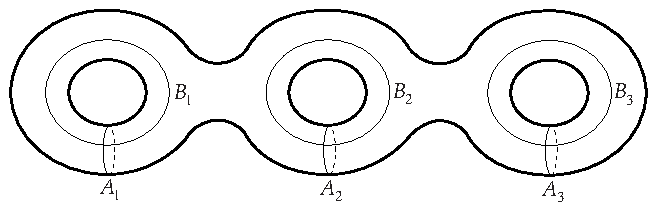
\includegraphics[width=0.8\linewidth]{figures/fig_9_1.pdf}
 \caption{$A$サイクルと$B$サイクルを描いた種数3の曲面。}\label{fig:9.1}
\end{figure}
\subsubsection*{Fuchsian群}
この構成では、まず世界面の計量を考える。Weyl変換によって世界面の曲率$R$を常に定数にできる、という定理がある。種数ゼロでは丸い球面、種数1では平坦なトーラス、高種数では一定の負曲率をもつ曲面が得られる。これらの単連結被覆空間も、同様に一定の曲率をもつ。このような単連結空間はちょうど3つある。丸い球面そのもの、平坦な平面（トーラスの被覆空間）、および計量
\begin{equation}
 ds^2=\frac{dz\,d\bar z}{(\operatorname{Im}z)^2}
 \tag{9.2.3}\label{eq:9.2.3}
\end{equation}
をもつ上半平面である。最後のものは、種数$g\geq2$のすべての曲面の被覆空間である。

これに対応して、種数$g\geq2$のすべての曲面は、上半平面をある離散群の作用で割ることによって得られる。この群の元は計量\hyperref[eq:9.2.3]{(9.2.3)}の等長変換でなければならず、これらの等長変換は実係数のMöbius変換$PSL(2,\mathbb R)$にほかならない。図\ref{fig:9.1}は、各ハンドルに$A$サイクルと$B$サイクルという閉曲線を描いた種数3の曲面を示している。これらの曲線は、点に縮められないという意味で非自明である。いずれかの曲線を1周すると、被覆空間では元の点には戻らず、それと同一視される点の1つに戻る。したがって各サイクルには$PSL(2,\mathbb R)$の元が対応し、それらも$A_i$または$B_i$と記す。

$A$サイクルと$B$サイクルは、どの閉経路もこれらを次々につないだものと同値（ホモトピック）であるという意味で完全である。実際には少し過剰であり、経路
\begin{equation}
 (A_1B_1^{-1}A_1^{-1}B_1)(A_2B_2^{-1}A_2^{-1}B_2)
 \cdots(A_gB_g^{-1}A_g^{-1}B_g)
 \tag{9.2.4}\label{eq:9.2.4}
\end{equation}
は1点に縮められるので、対応する積は恒等元でなければならない。モジュライを数えると、$PSL(2,\mathbb R)$の各元に3個の実パラメータがあって$6g$個となり、制約\hyperref[eq:9.2.4]{(9.2.4)}から3個、さらに$PSL(2,\mathbb R)$による全体の共役変換が同値な曲面を与えることから3個を引いて、合計$6g-6$個となる。

SchottkyとFuchsianのパラメータ表示は似ているが、性質はかなり異なる。とくに後者では複素構造がずっと見えにくく、それに応じて超弦への拡張も単純ではない。

\subsubsection*{周期行列}
トーラスのモジュラス$\tau$には、種数$g$において$g\times g$行列への自然な一般化がある。それを見るには、まずAbel微分、すなわち正則1形式が必要である。これらは、複素座標で
\begin{equation}
 \partial_{\bar z}\omega_z=0,\qquad\omega_{\bar z}=0
 \tag{9.2.5}\label{eq:9.2.5}
\end{equation}
を満たす世界面上の場$\omega_a$である。このような場はちょうど$g$個あり、さらに共役の関係を満たすものが$g$個ある。これはRiemann--Rochの定理\hyperref[eq:5.3.22]{(5.3.22)}から従う。Abel微分\hyperref[eq:9.2.5]{(9.2.5)}とその共役は演算子$P_0^T$の核にほかならず、この演算子に対するRiemann--Rochの定理は
\begin{equation}
 \dim\ker P_0^T-\dim\ker P_0=-\chi=2g-2
 \tag{9.2.6}\label{eq:9.2.6}
\end{equation}
である。演算子$P_0$は$h=0$のスカラー場$c,\tilde c$に作用するため、通常の勾配に帰着する。これには常に2つのゼロモード（$c=\text{定数}$または$\tilde c=\text{定数}$）があるので、$\dim\ker P_0^T=2g$となる。

1形式の線積分は座標不変な量である。したがってAbel微分の自然な基底は、
\begin{equation}
 \oint_{A_i}dz\,\omega_{zj}=\delta_{ij}
 \tag{9.2.7}\label{eq:9.2.7}
\end{equation}
によって定義される$\omega_{zi}$、$i=1,\ldots,g$である。すると周期行列
\begin{equation}
 \tau_{ij}=\oint_{B_i}dz\,\omega_{zj}
 \tag{9.2.8}\label{eq:9.2.8}
\end{equation}
が曲面の複素構造を特徴づける。種数1では$\omega_z$が定数なので、これは通常の$\tau$である。

$\tau_{ij}$が対称であることを示せるので、複素パラメータは$\tfrac12g(g+1)$個ある。$g=1,2,3$ではこれは複素モジュライの個数と等しいが、$g\geq4$ではそれより多い。したがって、すべての周期行列がRiemann面に対応するわけではない。テータ関数\hyperref[eq:7.2.36]{(7.2.36)}には自然な種数$g$への一般化があり、$\tau$は周期行列に、$\nu,n,a,b$は$g$成分ベクトルになる。

\subsubsection*{超楕円曲面}
ときに有用な別の記述を示そう。座標$z,y$をもつ空間$S_2\times S_2$を考える。複素パラメータ$Z_i$に対して、方程式
\begin{equation}
 y^2=\prod_{i=1}^{2k}(z-Z_i)
 \tag{9.2.9}\label{eq:9.2.9}
\end{equation}
で与えられる2次元部分多様体を考える。$z$座標に射影すると、$k$本の分岐切断を介してつながった2枚のシートがある。これによって$g=k-1$個のハンドルをもつ曲面ができる。分岐点は$z$に射影すると特異だが、曲面\hyperref[eq:9.2.9]{(9.2.9)}全体はそこで非特異であり、$y$が局所的によい座標となる。

曲面は$2k$個の複素数$Z_i$に依存するが、ここでもMöbius変換によってそのうち3個が冗長となり、$2k-3=2g-1$個の複素パラメータが残る。$g=1,2$ではこれはモジュライの数と等しいが、$g\geq3$ではモジュライの数のほうが多く、特別な曲面だけが\hyperref[eq:9.2.9]{(9.2.9)}の形をもつ。これらを超楕円曲面という。

\subsectionlink{世界面の縫い合わせと切断}\label{sec:9.3}
弦の振幅を解析するうえで有用なのは、高種数と低種数の振幅の間の関係である。その中心となるのが、低種数の曲面から高種数の曲面を作るための配管接合（plumbing fixture）である。あるパッチで座標$z_1$をもつ世界面$M_1$と、あるパッチで座標$z_2$をもつ世界面$M_2$を考える。これらを次のように接合して、新しい世界面$M$を作れる。$q$を複素パラメータとする。小さな$\epsilon$をとり、$M_1$から円板$|z_1|<(1-\epsilon)|q|^{1/2}$を、$M_2$から円板$|z_2|<(1-\epsilon)|q|^{1/2}$を切り取る。次に、
\begin{equation}
 z_1z_2=q
 \tag{9.3.1}\label{eq:9.3.1}
\end{equation}
を満たす点の対を同一視して、1つの曲面を作る。これを図\ref{fig:9.2}に示す。環状領域
\begin{equation}
 (1-\epsilon)^{-1}|q|^{1/2}>|z_1|>(1-\epsilon)|q|^{1/2}
 \tag{9.3.2}\label{eq:9.3.2}
\end{equation}
は図示したように縫い合わされる。この構成を表す記法の1つが
\begin{equation}
 M=M_1\infty M_2(z_1,z_2,q)
 \tag{9.3.3}\label{eq:9.3.3}
\end{equation}
である。この記法は、得られる曲面が局所座標の選択に依存することを強調している。異なる局所座標$z'_1,z'_2$を選べば、切り取る円が異なるため、接合した曲面も一般に異なる。2つのパッチが、単一の曲面$M_0$の異なる部分にあってもよい。その場合、配管接合による構成は曲面にハンドルを1つ加える。これを
\begin{equation}
 M=M_0 8(z_1,z_2,q)
 \tag{9.3.4}\label{eq:9.3.4}
\end{equation}
と記す。記号「$\infty$」と「$8$」は、2つの縫い合わせの過程を描き表す意図で用いている。実際にはパラメータ$q$は不要であり、$z'_1=z_1q^{-1/2}$、$z'_2=z_2q^{-1/2}$、$q'=1$とすると同値な曲面が得られる。座標パッチを固定したまま、$q$の関数としての振る舞いを論じるために$q$を導入すると便利なのである。

\begin{figure}[htbp]
 \centering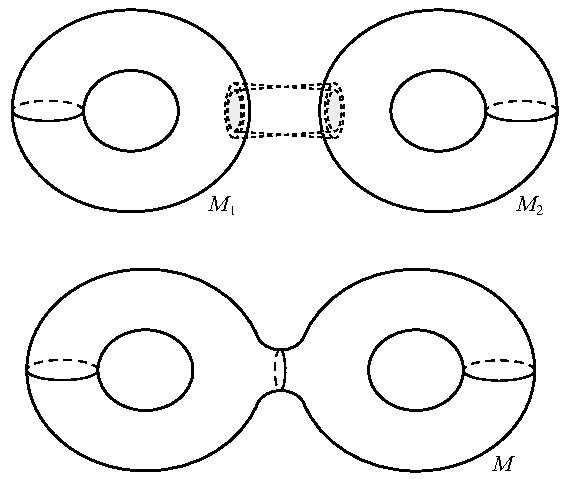
\includegraphics[width=0.8\linewidth]{figures/fig_9_2.pdf}
 \caption{2つの世界面のそれぞれから円板（網掛け部分）を取り除き、破線で示したように縁を貼り合わせて接合する。}\label{fig:9.2}
\end{figure}
この構成を逆にたどることもできる。任意のRiemann面$M$と、その上の自己交差しない任意の曲線$C$が与えられると、$C$の近傍で、$C$が$|z_1|=|z_2|=|q|^{1/2}$となる正則座標$z_1=z_2^{-1}$を常に見つけられる。$C$に沿って切断し（同一視$z_1z_2=q$を解き）、円板$|z_1|<|q|^{1/2}$と$|z_2|<|q|^{1/2}$を貼り込むと、$M_1$と$M_2$（または$M_0$）が得られる。縫い合わせ操作を行えば、これらから$M$を再構成できる。$C$に沿った切断によって曲面が非連結になるかどうかに応じて、操作は\hyperref[eq:9.3.3]{(9.3.3)}または\hyperref[eq:9.3.4]{(9.3.4)}となる。

図\ref{fig:9.2}の種数2の例で、$q\ll1$の場合を考えよう。図\ref{fig:9.3}(a)はこの場合の$M$を示している。重なり領域では、計量を$dz_1d\bar z_1$と$dz_2d\bar z_2$の間で滑らかに補間している。曲面は$|q|^{1/2}$程度の半径までくびれる。Weyl変換により、図\ref{fig:9.3}(b)に示すように半径が1程度に保たれる計量をとれる。Weyl変換は等方的に作用するため、ハンドルの長さが$-\ln|q|$程度まで大きくなる。ハンドル領域$|z_1|<1$、$|z_2|<1$は円筒
\begin{equation}
 \ln|q|<\operatorname{Im}w<0,\qquad w\cong w+2\pi
 \tag{9.3.5}\label{eq:9.3.5}
\end{equation}
と同値であり、$z_1=\exp(-iw)$、$z_2=q\exp(iw)$である。図\ref{fig:9.3}(c)は同じ曲面のもう1つの表現を示す。小さなハンドルを囲む環状領域$O(|q|)<|z|<O(1)$は、図\ref{fig:9.3}(b)の長い円筒と共形同値である。図\ref{fig:9.3}(a)から見ると、これは$M_2$全体を縮小するWeyl変換を行ったものと考えられる。

\begin{figure}[htbp]
 \centering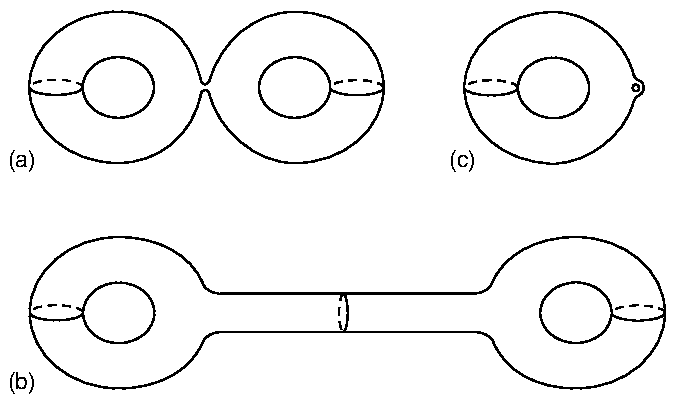
\includegraphics[width=0.8\linewidth]{figures/fig_9_3.pdf}
 \caption{サイクルが退化する種数2の曲面の3つの表現。}\label{fig:9.3}
\end{figure}
いずれの描像でも、$q\to0$極限で曲面が特別なものになることは明らかである。ハンドルがくびれる、または退化するという。これはモジュライ空間の境界の一例である。どのような発散もそこから生じるはずなので、モジュライ空間の境界は重要である。実際、すべての境界が、1つ以上のハンドルがくびれるこの形であることを見る。種数2の曲面では、単一のハンドルが退化する仕方がもう1つあり、$A$サイクルまたは$B$サイクルの1つがくびれる場合である。これは、2つのトーラスから「$\infty$」操作で作る代わりに、単一のトーラスから「$8$」操作で種数2の曲面を作り、$q\to0$とすることに対応する。

切断操作を繰り返すと、あらゆるRiemann面を3つの穿孔をもつ球面へと分解できる、という有用な事実がある。穿孔とは、指定された点とその近傍で定めた複素座標のことであり、配管接合を縫い込むために必要なデータである。言い換えると、あらゆるRiemann面は3つの穿孔をもつ球面を縫い合わせて構成できる。たとえば図\ref{fig:9.4}は、4つの頂点演算子をもつ種数2の曲面を構成する多数の方法のうち3つを示している。縫い合わせ操作ごとに複素モジュラス$q$が1つあり、図\ref{fig:9.4}の各構成では合計7個となる。これらは、種数2の曲面の$3g-3=3$個の複素モジュライと、4つの演算子の位置に対応する。

\begin{figure}[htbp]
 \centering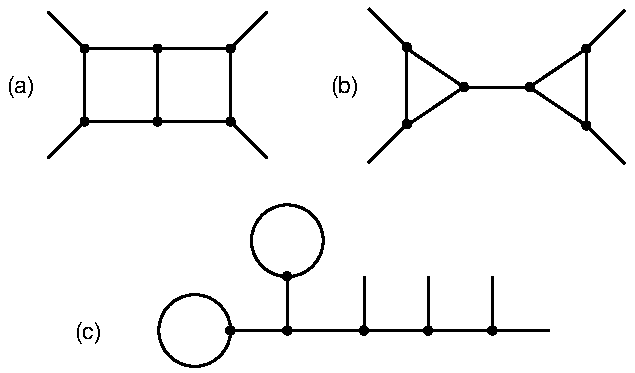
\includegraphics[width=0.8\linewidth]{figures/fig_9_4.pdf}
 \caption{4つの演算子をもつ種数2の曲面の、縫い合わせによる構成例。各頂点は3つの穿孔をもつ球面、各内線は配管接合による構成、各外線は頂点演算子を表す。}\label{fig:9.4}
\end{figure}
\subsubsection*{グラフによる分解}
図\ref{fig:9.4}のグラフはFeynman図を思わせる。ここでモジュライ空間のFeynman図に似た分解を述べよう。頂点は図\ref{fig:9.4}よりもかなり複雑で、任意の数の外線をもち、弦のループによる内部補正も含む。この構成の目的は、モジュライ空間の境界の性質を明示することにある。

主張は、モジュライ空間上の積分がFeynmanグラフの和で与えられる、というものである。グラフの各内部伝播関数は縫い合わせ操作を表し、縫い合わせパラメータ$q$を$|q|<1$のような標準的な領域で積分する。$n$点頂点は$n$個の穿孔をもつRiemann面を表す。後で見るように、頂点に含まれる曲面についてはモジュライ空間のある内部領域で積分し、さらに種数について和をとらなければならない。縫い合わせ操作は、縫い合わせる各点の特定の複素座標を参照するので、頂点の定義には各点での座標の選択も含めなければならない。$n$点頂点に現れる種数$g$のRiemann面の集合を$\mathcal V_{g,n}$と記す。外線は頂点演算子を表す。

この構成を具体的に示そう。3点頂点$\mathcal V_{0,3}$から始める。図\ref{fig:9.5}では、指定された3点と3つの縫い合わせ円をもつ球面として示してある。縫い合わせ円とは、それぞれの点に対応する複素座標での単位円である。この頂点を2つとり、それぞれから縫い合わせ円の1つの内部を取り除き、それらを円筒の両端に縫い合わせると、4点をもつ球面ができる。これは配管接合による構成と同値である。図\ref{fig:9.6}(a)のFeynmanグラフがこれに対応し、円筒の長さは、円周を$2\pi$に規格化すると$-\ln|q|$となる。$|q|<1$を積分し、他の2つのチャネルについて和をとっても、図\ref{fig:9.6}(b)に示すように、4点をもつ球面の積分領域の一部しか得られない。網掛けされた領域は含まれるが、網掛けのない内部領域は取り残される。

\begin{figure}[htbp]
 \centering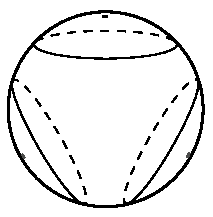
\includegraphics[width=0.65\linewidth]{figures/fig_9_5.pdf}
 \caption{球面上の3つの指定点と3つの縫い合わせ円をもつ、弦の3次頂点。}\label{fig:9.5}
\end{figure}
\begin{figure}[htbp]
 \centering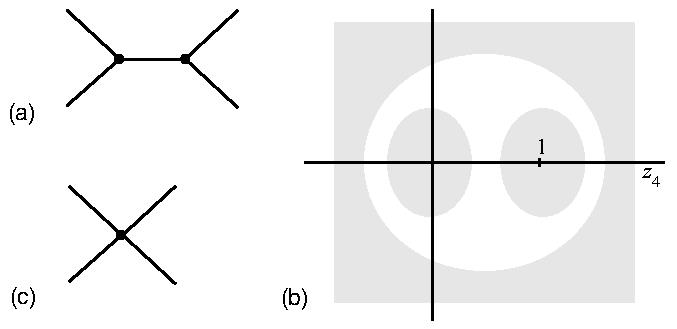
\includegraphics[width=0.8\linewidth]{figures/fig_9_6.pdf}
 \caption{(a) 4つの頂点演算子をもつ球面の構成。(b) このグラフが覆う$z$平面の領域。(c) 正しい振幅を得るために追加が必要な頂点。4つの穿孔をもつ球面を網掛けのない領域で積分する。}\label{fig:9.6}
\end{figure}
さらに具体化しよう。3次頂点について、球面上の点を標準的な位置$0,1,\infty$に置き、それぞれで座標系$z^{(0)},z^{(1)},z^{(\infty)}$を選ぶと、3つの縫い合わせ円は$|z^{(0,1,\infty)}|=1$となる。頂点が対称になるように、この選択は頂点演算子を置換する6つのMöbius変換の下で、位相を除いて不変でなければならない。可能な選択は多数あり、たとえば任意の定数$a$に対して
\begin{equation}
 z^{(0)}=\frac{az}{z-2},\qquad
 z^{(1)}=\frac{a(z-1)}{z+1},\qquad
 z^{(\infty)}=\frac{a}{2z-1}
 \tag{9.3.6}\label{eq:9.3.6}
\end{equation}
とできる。$a\geq3$では縫い合わせ円が重ならず、すべての$q\leq1$について配管接合が適切な曲面を与えることが保証される。読者が確かめられるように、2つの球面の$z^{(\infty)}$パッチと$z'^{(0)}$パッチをパラメータ$q$で縫い合わせると、$0,1,\tfrac12(1+a^2/q),\tfrac12(1-a^2/q)$に頂点演算子をもつ球面が得られる。これはMöbius変換により、$0,1,\infty$および
\begin{equation}
 z_4=\frac{(q-a^2)^2}{4a^2q}
 \tag{9.3.7}\label{eq:9.3.7}
\end{equation}
に頂点演算子をもつ球面と同値である。$q$が単位円板を走ると、$z_4$は図\ref{fig:9.6}(b)の外側の網掛け領域を覆う。外部の頂点演算子を置換すると、残りの2つの領域が得られる。$a$を小さくして網掛け領域を広げようとしても、やがて領域が重なって一部の曲面を二重に数える一方、依然として生成されない曲面が残る。これらが平面を過不足なく埋め尽くすことはない。そのため、4つの指定点をもつ球面を$z$平面の網掛けのない部分で積分した、明示的な4点頂点$\mathcal V_{0,4}$を加える必要がある。これだけでは$\mathcal V_{0,4}$の定義は完全ではない。$z_4$の各値に対し、各穿孔での座標も選ばなければならないからである。網掛け領域とそうでない領域の境界で滑らかにつながるように、その選択を行うことが常に可能である。図\ref{fig:9.6}(a)のFeynmanグラフはすべての漸近領域$z_4\to0,1,\infty$を含む一方、4点頂点には非退化な曲面だけが含まれることに注意しよう。したがって極限での振る舞いは、配管接合の$q\to0$極限によって明示的に与えられる。これがこの構成の有用な理由である。

別の例として、1つの頂点の2つの円を円筒の両端に縫い合わせると、1つの頂点演算子をもつトーラスができる。これはトーラスのモジュライ空間の$\operatorname{Im}\tau\to\infty$極限を覆うが、内部領域が取り残されるため、頂点領域$\mathcal V_{1,1}$として別途加えなければならない。

この構成は帰納的に拡張できる。縫い合わせ操作は、パラメータ
\begin{equation}
 r=3g+n-2
 \tag{9.3.8}\label{eq:9.3.8}
\end{equation}
を常に増加させる。出発点の3つの穿孔をもつ球面、頂点$\mathcal V_{0,3}$では$r=1$である。$8$操作は$r=r_0+1$を、$\infty$操作は$r=r_1+r_2$を与える。したがって$\mathcal V_{0,4}$と$\mathcal V_{1,1}$はいずれも$r=2$である。$r$について帰納的に$\mathcal V_{g,n}$を構成でき、それによって主張どおりモジュライ空間を覆えることが示されている。

より明示的な構成は次のとおりである（証明は参考文献にある）。任意のRiemann面には一意な最小面積計量が存在する。これは、すべての非自明な閉曲線（連続的に1点に縮められない曲線）の長さが少なくとも$2\pi$であるという制約のもとで、面積を最小にする計量として定義される。曲面上のすべての点は、長さがちょうど$2\pi$の非自明な閉曲線である、制約を飽和する測地線の少なくとも1つの上にある。互いに連続的に変形できる、すなわちホモトピー同値な、制約を飽和する測地線どうしは交差できない。ホモトピー同値な飽和測地線の各集合は、曲面上に帯（位相的には環）を作る。異なる帯は曲面を完全に覆い、互いに重なっていてもよい。帯の高さ$h$は、その境界となる2本の測地線の間の最短距離として定義する。穿孔のまわりを回る曲線を非自明とみなすと定めれば、最小面積計量の考えを穿孔のある曲面へも拡張できる。穿孔の近くでの最小面積計量は$dz\,d\bar z/z\bar z$という形であり、半径$2\pi$の半無限円筒である。したがって帯には2種類ある。曲面内部にある有限の帯と、穿孔を中心とし、曲面内部で終わる半無限の帯である。

この構成での$\mathcal V_{g,n}$を記述できるようになった。$n$個の穿孔をもつすべてのRiemann面をとる。ただし、最小面積計量で測ったすべての内部の帯の高さが$2\pi$未満であることを要求する。半無限円筒を、長さ$\pi$の短い管を残して切り落とし、その端に頂点演算子をもつ通常の単位円板を貼り込む。これらの頂点を用いると、Feynmanグラフの和はモジュライ空間をちょうど1回覆う。これらの最小面積曲面を縫い合わせたものも、最小面積曲面になることを示せる。高さ$2\pi$未満の帯は、頂点に明示的に含まれている。高さ$2\pi$より大きい帯は、短い管を縫い合わせる操作で生成される。その高さは、短い管からの$2\pi$に、配管接合からの$-\ln|q|$を加えたものであり、$q$を積分すると$2\pi$から$\infty$までを走る。長さの下限と高さの上限の制約により、退化する曲面は頂点に現れないことが保証される。したがって、それらは主張どおり、1つ以上の$q$がゼロになることによってのみ生じる。

\subsectionlink{CFTの縫い合わせと切断}\label{sec:9.4}
高種数のRiemann面を、低種数の曲面を縫い合わせて作るものとして記述した。経路積分の縫い合わせの性質を用いると、高種数の曲面上のCFTも同様に低次の振幅と関係づけられる。この関係を図\ref{fig:9.7}に描いてある。話を明確にするため、まず$q=1$の場合を論じよう。境界状態の完全系を挿入して、$M$上の経路積分を円$|z_1|=|z_2|=1$に沿って切り開く。次に、各境界状態を対応する局所演算子をもつ円板で置き換えると、切断前の世界面$M_1,M_2$が残る。結果の正確な形は
\begin{equation}
 \langle\cdots_1\cdots_2\rangle_M
 =\sum_{ij}\left\langle\cdots_1\mathcal A_i^{(z_1)}\right\rangle_{M_1}
 \mathsf G^{ij}\left\langle\mathcal A_j^{(z_2)}\cdots_2\right\rangle_{M_2}
 \tag{9.4.1}\label{eq:9.4.1}
\end{equation}
である。$M_1$上の任意の追加の挿入$\cdots_1$と、$M_2$上の任意の追加の挿入$\cdots_2$を許している。もちろん、これらは切断する円$|z_1|=1$および$|z_2|=1$の外側になければならない。基底には特定の正規直交条件を課していない。適切な逆計量$\mathsf G^{ij}$は、これから決める。ハンドルを置き換える挿入$\mathcal A_i,\mathcal A_j$は、それぞれ$z_1,z_2$座標系の原点にあるものとする。

\begin{figure}[htbp]
 \centering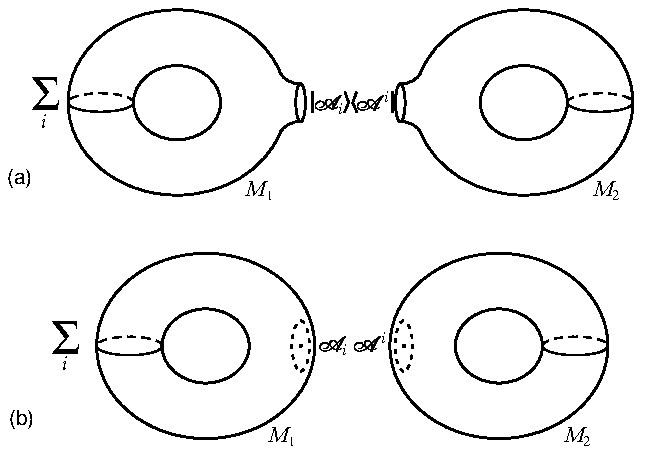
\includegraphics[width=0.8\linewidth]{figures/fig_9_7.pdf}
 \caption{(a) 境界状態の完全系を挿入して、$M$上の経路積分を切り開く。(b) 各状態を、局所演算子をもつ円板で置き換える。}\label{fig:9.7}
\end{figure}
次に、$M_2$が球面で、縫い合わせ座標$z_2$が$u$、$\cdots_2$が$z=0$にあるある局所演算子$\mathcal A_k$である場合を考えよう。配管接合から$z_1u=1$、球面から$zu=1$という同一視があるので、$z_1=z$を縫い合わせ領域全体へそのまま延長できる。縫い合わせた曲面$M$は、$z_1=0$に演算子$\mathcal A_k$を加えた$M_1$と同じである。すると式\hyperref[eq:9.4.1]{(9.4.1)}は
\begin{equation}
 \left\langle\cdots_1\mathcal A_k^{(z_1)}\right\rangle_{M_1}
 =\sum_{ij}\left\langle\cdots_1\mathcal A_i^{(z_1)}\right\rangle_{M_1}
 \mathsf G^{ij}\left\langle\mathcal A_j^{(u)}\mathcal A_k^{(z)}\right\rangle_{S_2}
 \tag{9.4.2}\label{eq:9.4.2}
\end{equation}
となる。2点関数$\langle\mathcal A_j^{(u)}\mathcal A_k^{(z)}\rangle_{S_2}$は、内積$\langle\!\langle j|k\rangle=\mathcal G_{jk}$にほかならない。したがって式\hyperref[eq:9.4.2]{(9.4.2)}から
\begin{equation}
 \mathsf G^{ij}\mathcal G_{jk}=\delta^i_k
 \tag{9.4.3}\label{eq:9.4.3}
\end{equation}
すなわち
\begin{equation}
 \mathsf G^{ij}=\mathcal G^{ij}
 \tag{9.4.4}\label{eq:9.4.4}
\end{equation}
が従う。つまり、球面上の2点関数によって定義される内積こそが、縫い合わせに対する正しい内積である。これで、$M_2$が任意の局所演算子をもつ球面である場合に、関係\hyperref[eq:9.4.1]{(9.4.1)}を導いた。状態・演算子同型により、任意の境界状態がこの方法で得られる。経路積分は局所的なので、結果は縫い合わせの領域だけに依存し、曲面の残りの部分には依存しない。したがって、任意の$M_2$および$\cdots_2$について成り立つ。

パラメータ$q$による縫い合わせは、$q=1$で局所座標$z_1$および$z'_2=z_2/q$を用いて縫い合わせることと同じである。したがって、$\mathcal A_j$をプライム付き座標系で表した式\hyperref[eq:9.4.1]{(9.4.1)}が得られ、$z_2$へ戻す共形変換から追加の因子
\begin{equation}
 \mathcal A_j^{(z'_2)}=q^{h_j}\bar q^{\tilde h_j}\mathcal A_j^{(z_2)}
 \tag{9.4.5}\label{eq:9.4.5}
\end{equation}
が生じる。結果は
\begin{equation}
 \langle\cdots_1\cdots_2\rangle_M
 =\sum_{ij}q^{h_j}\bar q^{\tilde h_j}
 \left\langle\cdots_1\mathcal A_i^{(z_1)}\right\rangle_{M_1}
 \mathcal G^{ij}\left\langle\mathcal A_j^{(z_2)}\cdots_2\right\rangle_{M_2}
 \tag{9.4.6}\label{eq:9.4.6}
\end{equation}
であり、共形ウェイトについて対角な基底を選んでいる。「$8$」操作の場合にも、$M$と$M_0$上の経路積分は同様に関係づけられる。
\begin{equation}
 \langle\cdots\rangle_M
 =\sum_{ij}q^{h_j}\bar q^{\tilde h_j}\mathcal G^{ij}
 \left\langle\cdots\mathcal A_i^{(z_1)}\mathcal A_j^{(z_2)}\right\rangle_{M_0}.
 \tag{9.4.7}\label{eq:9.4.7}
\end{equation}

1つ以上のハンドルの$q\to0$極限で与えられる、モジュライ空間の境界を改めて考えると興味深い。最も低い共形ウェイトの演算子が振る舞いを支配することがわかる。結果\hyperref[eq:9.4.6]{(9.4.6)}と\hyperref[eq:9.4.7]{(9.4.7)}はOPEに似ており、実際、$M_2$が球面で「$\cdots_2$」が1対の頂点演算子である場合、\hyperref[eq:9.4.6]{(9.4.6)}はOPEに帰着する。この類似は、極限を小さなハンドルの挿入として表す図\ref{fig:9.3}(c)からとくに明瞭にわかる。縫い合わせ関係は、演算子の積だけでなく、小さなハンドルや、世界面上の小さな円の中に縫い込める任意の変形も、局所演算子の和と同値であることを示す。結果\hyperref[eq:9.4.6]{(9.4.6)}はOPEの美しい一般化である。$M_1$から見ると、$z_1=0$の近くに$M_2$の小さな複製が貼り込まれている。これは、$\langle\mathcal A^i\cdots_2\rangle_{M_2}$を係数関数として、局所演算子$\mathcal A_i$で展開できる。$M_2$から見ると、$z_2=0$の近くに$M_1$の小さな複製が貼り込まれており、係数関数$\langle\cdots_1\mathcal A_i\rangle_{M_1}$を用いて局所演算子$\mathcal A^i$で展開される。

あらゆるRiemann面は3つの穿孔をもつ球面へと分解できると論じた。したがって縫い合わせによる構成は、すべての振幅を球面上の3点振幅に関係づける。後者は本質的に演算子積係数であり、これらがCFTを定義するデータである。今後、CFTの間の多くの同値性に出会うことになる。すでに$T$双対性を見たが、ボソン化（第10章）も顕著な例である。縫い合わせによる構成は、2つの理論が同じであるための判定基準を与える。それは、状態（または局所演算子）の間に1対1の対応があり、OPEが一致することである。\footnote[1]{第2.5節の自由場の例のように、$T_{ab}$の役割を果たしうる$(2,0)$と$(0,2)$の場の組が複数ある場合には、そのうちどれがエネルギー運動量テンソルなのかを指定する必要がある。この選択が演算子の共形変換を決め、その変換は縫い合わせ関係に暗黙に入っていることに注意しよう。}実際、第15章で示すように、一次場の演算子積だけで他のすべての場の演算子積が決まる。

この見方をさらに調べよう。曲面は多くの異なる曲線の組に沿って切断できるので、縫い合わせ関係が常に$M$上の期待値に対して同じ結果を与えるための整合性条件がなければならない。まず、切断曲線$C$の無限小変化を考える。$M$を不変に保つ一般の無限小変化は、縫い合わせに用いる座標の無限小変化
\begin{align}
 z'_1&=z_1+\sum_{n=-\infty}^{\infty}\epsilon_n z_1^{n+1},
 \tag{9.4.8a}\label{eq:9.4.8a}\\
 z'_2&=z_2-\sum_{n=-\infty}^{\infty}\epsilon_{-n}q^{-n}z_2^{n+1}
 \tag{9.4.8b}\label{eq:9.4.8b}
\end{align}
によって得られる。すると、縫い合わせて得られる式の差は
\begin{equation}
 \begin{aligned}
 &\mathcal A_i^{(z'_1)}\mathcal G^{ij}\mathcal A_j^{(z'_2)}
 -\mathcal A_i^{(z_1)}\mathcal G^{ij}\mathcal A_j^{(z_2)}\\
 &\quad=-\sum_{n=-\infty}^{\infty}\epsilon_n
 \Bigl[L_n\cdot\mathcal A_i^{(z_1)}\mathcal G^{ij}\mathcal A_j^{(z_2)}
 -\mathcal A_i^{(z_1)}\mathcal G^{ij}L_{-n}\cdot\mathcal A_j^{(z_2)}\Bigr]
 +(\mathrm{anti})
 \end{aligned}
 \tag{9.4.9}\label{eq:9.4.9}
\end{equation}
に比例する。ここでは共形変換\hyperref[eq:2.9.6]{(2.9.6)}を用いた。「anti」は、$\epsilon_n\to\epsilon_n^*$、$L_n\to\tilde L_n$と置き換えた同じ形を表す。括弧内の量が消えることは、式\hyperref[eq:9.4.4]{(9.4.4)}の導出と同様の議論によって示せる。これは、生成子を定義する周回積分を、縫い合わせたハンドルを通して引き抜ける、ということにほかならない。$L_n$から$L_{-n}$への変化は座標の反転による。保存電荷に対する他のすべての周回積分も、同様に通り抜けさせられる。

連続変形で結ばれない曲線の組もある。球面上の4点振幅は、異なる演算子の対を囲む曲線に沿って切断することで、3点関数を用いて書ける。異なる縫い合わせの間で結果が等しいことは、図\ref{fig:2.8}に示したOPEの結合律である。

もう1つの例はトーラスである。$A$サイクル、$B$サイクル、あるいは他の任意の自己交差しない閉曲線に沿って切断することで、トーラスを球面へと帰着できる。同一視を伴う平面の言葉でいうと、$(\sigma^1,\sigma^2)=(0,0)$から出発する閉曲線$C$は、それと同一視される点
\begin{equation}
 2\pi(m,n)
 \tag{9.4.10}\label{eq:9.4.10}
\end{equation}
で終わらなければならない。同じ$m,n$の値をもつすべての曲線は互いに連続的に変形できるので、異なる$m,n$の曲線で縫い合わせる場合の関係を考えればよい。非自明で自己交差しない曲線の場合、$m,n$は互いに素でなければならないことを示せる。したがって、$mp-nq=1$を満たす整数$p,q$が存在する。するとモジュラー変換
\begin{equation}
 (\sigma^1,\sigma^2)=(\sigma'^{1},\sigma'^{2})
 \begin{bmatrix}m&n\\q&p\end{bmatrix}
 \tag{9.4.11}\label{eq:9.4.11}
\end{equation}
があり、曲線$C$は
\begin{equation}
 (\sigma'^{1},\sigma'^{2})=2\pi(1,0)
 \tag{9.4.12}\label{eq:9.4.12}
\end{equation}
へ戻る。これは$A$サイクルである。したがって、一般の非自明で自己交差しない曲線に沿って切断することは、モジュラー同値な$\tau$の値に対して$A$サイクルに沿って切断することと同値である。ゆえに、縫い合わせによる構成の整合性はモジュラー不変性と同値である。

縫い合わせ曲線の任意の組は、2種類の操作を繰り返すことで、他の任意の組へ移せる。その操作は、球面上の4点の結合律変換と、1つの頂点演算子をもつトーラス上のモジュラー変換である。図\ref{fig:9.4}を見ると、これがもっともらしいことがわかる。たとえば図\ref{fig:9.4}(a)と図\ref{fig:9.4}(b)は1つの結合律条件で結ばれる。結合律を繰り返し適用すると、すべてのループが1ループ1点関数で表された図\ref{fig:9.4}(c)の形に縫い合わせを変えられる。したがって、これらが、任意の演算子積係数の集合が矛盾のない共形場理論を定義するための条件である。双対性の制約を解くこの研究方針は、共形ブートストラップと呼ばれる。第15章で論じるように、追加の制約を導入した場合にのみ実行されている。

本節の考察はすべて、境界をもつ世界面にも拡張される。その場合、退化するハンドルに加えて、退化する帯が現れることもある。整合性条件はこの場合にも一般化されている。


% 原文PDF327の第9.5節見出しからPDF350末まで。
\subsectionlink{一般の振幅}\label{sec:9.5}

これで、一般の弦振幅の整合性を理解するために必要な要素が、すべてそろった。

モジュライ空間のグラフによる分解を与えたので、縫い合わせ形式によって、一般の弦振幅を図式的に表せる。まず、配管接合から得られる伝播関数を考えよう。モジュラス $q$ に対するゴースト挿入は
\begin{equation}
\oint\frac{dz}{2\pi i}\,b_{z_1z_1}
\left.\frac{\partial z_1}{\partial q}\right|_{z_2}
=\frac{b_0}{q}
\tag{9.5.1}\label{eq:9.5.1}
\end{equation}
であり、同様に $\bar q$ に対しては $\widetilde b_0/\bar q$ である。これらの挿入を含め、縫い合わせの表式 (9.4.6) を用いると、伝播関数に付随する因子は
\begin{equation}
\int_{|q|<1}\frac{d^2q}{q\bar q}\,
q^{\alpha'(k_i^2+m_i^2)/4}
\bar q^{\alpha'(k_i^2+\widetilde m_i^2)/4}
\mathcal G^{ij}b_0\widetilde b_0
=\frac{8\pi\delta_{m_i^2,\widetilde m_i^2}\mathcal G^{ij}b_0\widetilde b_0}
{\alpha'(k_i^2+m_i^2-i\epsilon)}
\tag{9.5.2}\label{eq:9.5.2}
\end{equation}
となる。$n$ 弦結合は、縫い合わせ構成の頂点に現れる曲面に頂点演算子を挿入することで与えられる。
\begin{equation}
g(i_1,\ldots,i_n)=\sum_g\int_{\mathcal V_{g,n}}d^mt\,
\left\langle\prod_{k=1}^{m}B_k
\prod_{l=1}^{n}\widehat{\mathcal V}_{i_l}\right\rangle_g.
\tag{9.5.3}\label{eq:9.5.3}
\end{equation}
ここで $m=6g+2n-6$ はモジュライの数である。結合 (9.5.3) と伝播関数 (9.5.2) から作られる Feynman グラフは、弦振幅全体を再現する。ラベル $i$ は、ここでも各弦の状態と運動量を表す。第9.1節の木振幅は、この構造を具体的に示している。

最初の問題は振幅の有限性である。低次のさまざまな例と同様に、発散はモジュライ空間の境界からしか生じないと主張する。モジュライが有限の値をとるとき、縫い合わせ公式は無限個の弦状態の和を与えるが、この和は収束する。究極的には、量子状態を完全系で展開しているだけだからである。実際には、収束が保証されるのはユニタリな CFT に限られるが、弦の CFT の非ユニタリな部分は、十分扱いやすい。$X^0$ の CFT はユニタリな CFT からの解析接続で定義され、ゴースト CFT は Faddeev--Popov 行列式を生成するだけなので、適切なゲージを選んでいれば有限である。境界は、今や各伝播関数の $q\to0$ 極限として明示されており、積分 (9.5.2) はこれまでに何度も出会ったものである。これは解析接続によって定義され、通常の場の理論の伝播関数を与える。したがって特異性は伝播関数の極だけであり、中間状態に質量殻上の粒子が生成されることを表す。特に、これらは短距離ではなく長距離の発散である。

もう一つの問題はユニタリティである。4点木振幅については、これをかなり詳しく調べた。一般の振幅を Feynman 図の形にしたので、組合せ論を詳しく展開する代わりに、図式展開のユニタリティに関する場の理論の標準的な結果を引用するだけにしよう。また、第9.1節の最後で示した、中間状態の和が物理的状態の和に帰着するという証明も、場の理論と同様に一般化される。

まとめると、弦理論の摂動的有限性とユニタリティに関わる問題は、十分理解されているように見える。再び注意しておくと、26個の平坦な方向を仮定したのではなく、$d$ 個の平坦な方向と、中心電荷 $26-d$ をもつ正ノルムのコンパクト CFT だけを仮定した。もちろん、ボソン弦の平坦時空の S 行列のユニタリティについての議論は、いくらか形式的である。平坦時空は理論の解ではないからである。まずタキオン不安定性があり、さらにループによって宇宙項が誘起される。

光円錐ゲージに基づく、弦理論の有限性とユニタリティへの別のアプローチも、広く発展してきた。このゲージは共変性を放棄するが、いくつかの利点がある。モジュライ空間をかなり明示的に記述でき、振幅を、光円錐時間 $x^+$ に関して局所的な Hamiltonian をもつ場の理論の形で表せる。その摂動論が共変な摂動論と等価であることを示すことによって、共変性も確立されている。

\subsubsectionlink*{弦の発散}

先へ進む前に、弦の発散が長距離の効果であるという点を、もう少し詳しく説明しよう。$n$ 個の頂点演算子を含む1ループ振幅を考え、図9.8(a)のように $\tau$ を固定したまま、$m$ 個の演算子が集まる極限を取る。弦のループはもちろん重力を含み、図9.8(a)は、相互作用頂点が時空内で集まると紫外発散を生じた、図1.1(c)の重力子ループを思わせる。この弦振幅にも確かに発散があるが、それは時空の短距離ではなく、長距離から来る。図9.8(b)は共形的に等価な描像であり、$m$ 個の頂点演算子は長い円筒によってトーラスの残りの部分につながっている。この円筒を切り開いて状態の完全系を挿入すると、通常の表式 (9.5.2) が得られ、$q\to0$ が頂点演算子の一致する極限に対応する。したがって特異性は、時空の長距離を伝播することによる通常の極だけである。ここでも共形不変性は、世界面上の短距離を時空の長距離へ変える。

\begin{figure}[tbp]
\centering
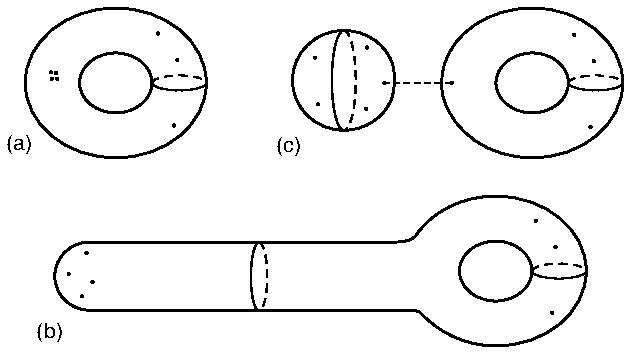
\includegraphics[width=0.82\linewidth]{figures/fig_9_8.pdf}
\caption{(a) $n$ 個の頂点演算子をもつトーラスで、そのうち $m$ 個が集まる極限。(b) 共形的に等価な描像。$m$ 個の頂点演算子は長い円筒の先端にある。(c) $m+1$ 個の頂点演算子をもつ球面と、$n-m+1$ 個をもつトーラスの積による縫い合わせ構成。}
\label{fig:9.8}
\end{figure}

$m=n$ と $m=n-1$ の場合には、特別な問題が生じる。$m=n$、すなわちすべての頂点演算子が集まる場合、運動量保存によって $k^\mu$ はゼロに強制される。質量のない状態では、その極は $1/0$ となり、通常の解析接続は役立たない。運動量保存により、振幅は質量のない極の真上に固定されるからである。これは第7.4節と同じタドポールであり、解決法も同じく背景場の補正である。ここでの発散は、一つの頂点演算子を含むトーラス振幅に比例する。

もう一つの問題となる場合、$m=n-1$ では、一つ、例えば $\mathcal V_n$ を除くすべての頂点演算子が集まる。運動量保存は、円筒を流れる運動量が $k^\mu=-k_n^\mu$ であることを要求する。しかし共形不変性は $k_n^2=-m_n^2$ を要求するので、$m_j^2=m_n^2$ の中間状態に対しては、中間運動量が極の真上に固定される。ここでも場の理論に同様の発散があり、図9.9に示した内部伝播関数は $1/0$ となる。この発散は、内部線 $j$ の質量が、質量殻上の外部粒子 $n$ の質量と同じときに必ず起こる。解釈は単純である。ループは粒子 $n$ の質量に対する輻射補正を表す。S 行列は、輻射補正を含めた\textbf{真の}質量殻上に外部運動量を取って定義され、その場合にはこの赤外発散は再びなくなる。ここで問題なのは、ループ内部の何らかの紫外発散ではなく、星印を付けた伝播関数の赤外発散であり、質量補正が有限であっても現れることに注意しよう。

\begin{figure}[tbp]
\centering
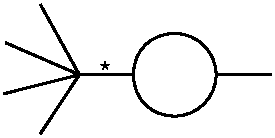
\includegraphics[width=0.57\linewidth]{figures/fig_9_9.pdf}
\caption{$m=n-1$ の場合に対応する場の理論のグラフ。運動学によって、星印を付けた伝播関数は発散する。ループによる有限の質量シフトと解釈される。}
\label{fig:9.9}
\end{figure}

弦の場合の解決法も同じである。頂点演算子に現れる運動量は、真の物理的質量に対応していなければならない。これは一般に、二乗が常に $1/\alpha'$ の整数倍だった、木レベルの質量とは同じでない。ある種の質量のない場、特にゲージボソンについては、ゲージ不変性が、あらゆる次数で質量がないままであることを保証する。なお、質量をもつ状態の質量シフトは通常複素数になる。これらの状態は、より軽い弦状態へ崩壊する不安定性をもつからである。

ここには一つ疑問がある。初めの方で、弦理論の整合性、すなわち世界面理論が共形不変であるという条件は、ベータ関数 (3.7.14) がゼロになることを要求すると見た。このベータ関数は高種数の曲面について何の情報も含まず、木レベルの弦の場の方程式に対応する。ループ補正を受けた背景のまわりで展開しようとすると、何が起きるのだろうか。実際には、すべてがちょうどうまく働く。図9.8の危険な極限は、発散だけでなく共形アノマリーも生む。これを直観的に見るために、その極限を図9.3(c)のように、球面に小さなハンドルを貼り付けたものとして描こう。小さなハンドルは局所演算子の級数で表せ、特に質量のないレベルからは
\begin{equation}
\partial X^\mu\bar\partial X_\mu\,\frac{dq\,d\bar q}{q\bar q}
\tag{9.5.4}\label{eq:9.5.4}
\end{equation}
がある。ここで、ハンドルの大きさが $a$ より大きいと要求して、座標不変な形で発散を切り落とす。すなわち、球面の計量が $dz\,d\bar z\,e^{2\omega}$ であるとき、$|q|e^\omega>a$ とする。積分 (9.5.4) の下限は
\begin{equation}
-4\pi\partial X^\mu\bar\partial X_\mu\ln(ae^{-\omega})
\tag{9.5.5}\label{eq:9.5.5}
\end{equation}
を与える。こうして計量の Weyl 因子への新たな依存性が生じ、これはシグマ模型の Weyl アノマリー $\beta_{\mu\nu}^G$、式 (3.7.14)、を補正する。Weyl 不変な理論を得るには、背景場が\textbf{弦のループ補正をすべて含めた} Weyl 不変性の条件、または等価に BRST 不変性の条件を満たさなければならない。シフトした背景からの Weyl アノマリーが、小さなハンドルからのものを打ち消す。これが \textbf{Fischler--Susskind 機構}である。図9.3(c)から、この発散と Weyl アノマリーは世界面の紫外効果と考えられる。ただし、通常の場の短波長の揺らぎによるものではなく、小さな位相幾何学的揺らぎによる。どのような種数でも、\textbf{固定した} Riemann 面上では局所的構造はトポロジーの影響を受けないことを強調しておく。発散と Weyl アノマリーを生むのは、Riemann 面についての積分である。

これは、伝播関数の相殺を用いた議論の破綻とみなすこともできる。運動学が振幅を極に固定するため、BRST 変分で生じうる表面項を除くのに解析接続を使えない。実際、その表面項は現れ、Weyl アノマリー (9.5.5) に対応する。ループ補正された背景では、背景のシフトによる BRST アノマリーが、モジュライ空間の境界によるものを打ち消す。弦特有の技術的な諸要素がすべてかみ合って、整合的な時空描像を与えるのである。

これを弦の摂動論で実行するのはかなり煩雑だが、幸い、必要になることはまれである。第一に、大部分の超対称理論では背景は補正されない。第二に、弦理論の長距離物理の解析は、普通は二段階で進めるのが最も効率的である。まず弦理論を用いて低エネルギー有効作用の形を導き、次に長距離では有効場の理論を用いる。そうすれば、弦の段階で赤外発散を扱う必要はない。今の場合、タドポールは有効作用中のポテンシャルエネルギー項
\begin{equation}
\delta\boldsymbol S=-\sum_\chi\Lambda_\chi
\int d^dx\,(-G)^{1/2}e^{-\chi\Phi}
\tag{9.5.6}\label{eq:9.5.6}
\end{equation}
を意味する。$\Lambda_\chi$ は Euler 数 $\chi$ からのタドポールであり、作用の $\Phi$ 依存性は $e^\Phi$ が弦結合であることから従う。重力子とディラトンそれぞれのタドポールは、いくらか手間をかければ弦振幅から取り出せる。

同じ考え方は、質量シフトによる頂点演算子の補正や、質量のない粒子を含む理論の排他的振幅に現れるものなど、他の赤外発散にも拡張される。弦理論は長距離で場の理論に帰着するので、これらの場の理論の発散は、対応する弦理論の振幅にも現れなければならない。繰り返し強調すると、場の理論の紫外発散は一般に、その理論の有効範囲の根本的な限界を意味するが、赤外発散は通常、それ以外は完全に整合的な理論に対して、単に誤った問いを立てていることを意味する。誤った背景、誤った質量、包括的断面積を問うべきところで排他的断面積を問うこと、などである。弦理論でのこのような発散も、まさに場の理論と同じように扱うべきである。

得られたことを振り返ろう。ボソン弦に特有の問題を除けば、S 行列は有限かつユニタリである。基本となる機構はモジュラー不変性であり、時空のゲージ不変性を損なわずに紫外発散を切り落とす。もちろん、平坦時空のまわりの弱結合摂動論で弦理論が意味をもつとわかっただけでは、とても十分とはいえない。摂動論を超えて理論が意味をもつことを知り、非摂動的補正を計算する何らかの手段が欲しい。また、短距離における時空の本性について、弦理論が何を示唆するかも知りたい。本章の残りでは、これらの方向でなされてきた試みのいくつかを簡単に述べる。

\subsectionlink{弦の場の理論}\label{sec:9.6}

弦理論でここまで採ってきた方法と、量子場の理論の定式化とを比較するのは興味深い。世界面の経路積分は粒子の経路の和に相当し、しばしば\textbf{第一量子化}の記述と呼ばれる。一方、量子場の理論では、時空の場についての経路積分、またはそれと等価な Hamiltonian 形式から出発する。代わりに、量子場の摂動論を第一量子化の形で展開することもできる。その場合には、$n$ 本の粒子の経路が終わる時空点として、相互作用頂点を明示的に導入する必要がある。弦理論では、この第二段階は必要ない。特別な点はなく、トポロジーについての和が相互作用を生む。しかし、得られるのは摂動展開だけであり、この展開に含まれない重要な現象もある。標準模型では、クォークの閉じ込めや、弱い相互作用による有限温度でのバリオン数の非保存がその例である。これらが摂動級数の再総和に含まれるといっても、有用な意味はないようであり、むしろ、より一般的な理論の定式化を必要とする。

前節では弦振幅を、無限成分の場の理論の摂動論に見える、伝播関数と頂点の形で表した。これを、無限個の時空場についての経路積分から導くことはできるだろうか。また、ゲージ不変性と一般座標不変性を拡張し、理論の形を決定する何らかの原理があるだろうか。これが\textbf{弦の場の理論}の主題である。ここでは、ごく少数の考え方、特にここまでのアプローチに近いものを概説するにとどめる。詳細は文献を参照してほしい。

弦の波動汎関数 $\Psi[X]$ を、場の演算子、または等価に経路積分の積分変数へ昇格させるべきだという推測から始めよう。いわゆる第二量子化である。$\Psi[X]$ は、弦が時空内に描く曲線 $X^\mu(\sigma)$ に依存し、大まかにいえば、その配置の弦を生成または消滅させる。しかし、もっと正確にする必要がある。例えば $\Psi$ には曲線の再パラメーター化に対する不変性を要求すべきだろうか。また、Polyakov 計量 $g_{ab}$ にも依存させるべきだろうか。Faddeev--Popov ゴーストを含めた BRST 不変な理論の形から始め、そこから第二量子化すると、はるかにうまく進むようである。交換関係から $b$ と $c$ は互いに共役であり、$\widetilde b$ と $\widetilde c$ も同様である。したがって、例えば $c,\widetilde c$ を座標として扱えば、波動汎関数は $\Psi[X,c,\widetilde c]$ となる。そして、そのようなすべての汎関数についての経路積分
\begin{equation}
\int[d\Psi]\exp(i\boldsymbol S[\Psi])
\tag{9.6.1}\label{eq:9.6.1}
\end{equation}
を考える。まず開弦について、一つの具体的なアプローチを述べよう。

どのような対称性原理が弦の作用を制限するだろうか。頂点演算子とヌル状態の研究から、任意の汎関数 $\Lambda$ に対する対称性
\begin{equation}
\delta\Psi=Q_{\mathrm B}\Lambda
\tag{9.6.2}\label{eq:9.6.2}
\end{equation}
を推測できる。この不変性をもつ極めて単純な作用がある。
\begin{equation}
\boldsymbol S_0=\frac12\langle\!\langle\Psi|Q_{\mathrm B}|\Psi\rangle.
\tag{9.6.3}\label{eq:9.6.3}
\end{equation}
運動方程式は単に
\begin{equation}
Q_{\mathrm B}\Psi=0
\tag{9.6.4}\label{eq:9.6.4}
\end{equation}
である。

これが妥当であることを見る一つの方法は、弦の各内部状態に一つずつ対応する、無限個の通常の場で弦の場 $\Psi$ を展開することである。内部モード、すなわち重心 $x^\mu$ 以外のすべてに対する波動関数の完全系を $\Psi_i[X',c,\widetilde c]$ としよう。一般の状態は
\begin{equation}
\Psi[X,c,\widetilde c]
=\sum_i\Phi_i(x)\Psi_i[X',c,\widetilde c]
\tag{9.6.5}\label{eq:9.6.5}
\end{equation}
と展開でき、展開係数は残りの変数 $x^\mu$ の関数となる。弦の場の経路積分は、成分関数に対する経路積分の無限積
\begin{equation}
\int[d\Psi]\longrightarrow\prod_i\int[d\Phi_i]
\tag{9.6.6}\label{eq:9.6.6}
\end{equation}
になる。いつものように、基底状態の汎関数 $\Psi_0$ から出発し、上昇演算子によって残りの状態を作れる。例えば、最初の二つのレベルのすべての状態を残すと、
\begin{equation}
\begin{split}
\Psi=\bigl[&
\varphi(x)+A_\mu(x)\alpha_{-1}^\mu+B(x)b_{-1}
+C(x)c_{-1}+\varphi'(x)c_0\\
&+A'_\mu(x)\alpha_{-1}^\mu c_0+B'(x)b_{-1}c_0
+C'(x)c_{-1}c_0+\cdots\bigr]\Psi_0.
\end{split}
\tag{9.6.7}\label{eq:9.6.7}
\end{equation}
ここで $\varphi$ はタキオン場、$A_\mu$ はゲージ場であり、$B,C$ は時空ゲージ対称性に付随する Faddeev--Popov ゴースト場である。プライムの付いた場はすべて、ゲージ変換で消せるか、補助場である。補助場とは、微分方程式ではなく代数方程式を満たし、消去できる場をいう。すると、対称性 (9.6.2) が $A_\mu$ の通常のゲージ変換を含み、作用が $\varphi$ に対して Klein--Gordon 形、$A_\mu$ に対して Maxwell 形であることを確かめられる。したがって BRST による弦の場の形式は、時空のゲージ不変性を非常に簡潔に一般化している。

\begin{figure}[tbp]
\centering
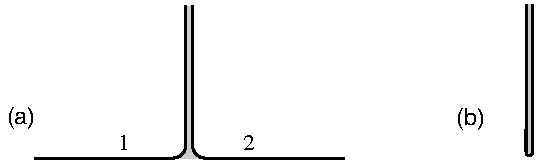
\includegraphics[width=0.74\linewidth]{figures/fig_9_10.pdf}
\caption{(a) $\Psi_1$ の右半分と $\Psi_2$ の左半分を畳み込む $\Psi_1*\Psi_2$。陰を付けた領域の経路積分として定義し、その幅をゼロにすると考えてよい。(b) $\Psi$ の右半分と左半分を畳み込む $\int\Psi$。}
\label{fig:9.10}
\end{figure}

相互作用も、かなりうまく構成できる。図9.10(a)に描いた汎関数積分によって、弦の場の積 $\Psi_1*\Psi_2$ を定義する。これは $\Psi_1$ の右半分と $\Psi_2$ の左半分の重なりを取る。また、図9.10(b)のように、単一の弦の波動汎関数の右半分と左半分の重なりを与える演算 $\int$ も定義する。相互作用する理論を作るため、ゲージ変換に非線形項を加える。
\begin{equation}
\delta\Psi=Q_{\mathrm B}\Lambda+g\Psi*\Lambda-g\Lambda*\Psi.
\tag{9.6.8}\label{eq:9.6.8}
\end{equation}
$*$ 積は結合的であり、積分路の議論により、$Q_{\mathrm B}$ は微分として
\begin{equation}
Q_{\mathrm B}(\Psi_1*\Psi_2)
=(Q_{\mathrm B}\Psi_1)*\Psi_2+\Psi_1*(Q_{\mathrm B}\Psi_2)
\tag{9.6.9}\label{eq:9.6.9}
\end{equation}
と作用することを示せる。これらから、対称性 (9.6.8) が閉じることが従う。巡回性
\begin{equation}
\int\Psi_1*\Psi_2=\int\Psi_2*\Psi_1
\tag{9.6.10}\label{eq:9.6.10}
\end{equation}
を用いると、不変な作用を
\begin{equation}
\boldsymbol S=\frac12\int\Psi*Q_{\mathrm B}\Psi
+\frac{2g}{3}\int\Psi*\Psi*\Psi
\tag{9.6.11}\label{eq:9.6.11}
\end{equation}
と書ける。$\Psi$ を、対応する頂点演算子 $\mathcal V_\Psi$ をもつ半円板に置き換えて、CFT によって書くのも有用である。
\begin{equation}
\boldsymbol S=\frac12
\langle\mathcal V_\Psi Q_{\mathrm B}\cdot\mathcal V_\Psi\rangle_{D_2}
+\frac{2g}{3}\langle
\mathcal V_\Psi\mathcal V_\Psi\mathcal V_\Psi\rangle_{D_2}.
\tag{9.6.12}\label{eq:9.6.12}
\end{equation}
頂点演算子の位置と共形座標枠は式 (9.6.12) に明示していないが、図9.11のとおりである。三つの頂点演算子の半円板を円板の中に収めるため、$z^{2/3}$ 写像を用いる。この作用は重要な確認を通過する。円板上の経路積分がゼロでないのは、挿入の全ゴースト数が $Q^{\mathrm g}=3$ の場合だけである。物理的状態の頂点演算子はすべてゴースト数1をもつので、作用 (9.6.12) の両項はゼロでない。作用 (9.6.11) は不変なので、ゲージ場に対して非 Abel な Yang--Mills 作用に帰着すると期待でき、実際にそうなる。

\begin{figure}[tbp]
\centering
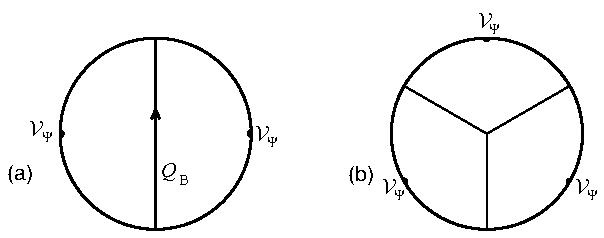
\includegraphics[width=0.78\linewidth]{figures/fig_9_11.pdf}
\caption{弦の場の作用の CFT 表現。(a) 運動項、(b) 相互作用。各頂点演算子を囲む通常の半円を扇形へ変えるため、$z^{2/3}$ の共形変換を用いる。}
\label{fig:9.11}
\end{figure}

Siegel ゲージは $b_0\Psi=0$ である。運動項の作用では、$Q_{\mathrm B}$ のうち $c_0L_0$ の項だけが残る。成分ごとに $L_0\propto p^2+m^2$ なので、これは電磁力学でおなじみの共変ゲージに相当する。伝播関数
\begin{equation}
\int_0^\infty dt\,\exp(-tL_0)=L_0^{-1}
\tag{9.6.13}\label{eq:9.6.13}
\end{equation}
は、任意の長さの帯についての積分にすぎない。頂点は図9.11(b)から扇形を取り除いたもので、三本の帯の端を「Y」字に結合する。これは Riemann 面の和として記述した開弦理論と等価であり、特にモジュライ空間を完全に一度だけ覆うことも示されている。一方で、これは驚くべきことではない。弦の場の理論には時空ゲージ不変性 (9.6.8) があるので、ヌル状態は S 行列から脱結合する。われわれは、ヌル状態の脱結合が弦振幅の形を決め、モジュライ空間を完全に覆う必要性も含むと論じた。そうでなければ、全微分項がヌル状態の結合を与えてしまう。他方で、モジュライ空間は複雑であり、明示的な記述はほとんど知られていない。この弦の場の理論が与える、Feynman グラフについての和と、各グラフの帯の長さについての積分による記述は、弦の場の理論による構成よりわずかに前に、数学者たちによって発見された。\footnote[2]{物理に動機付けられたモジュライ空間の別の記述は、光円錐ゲージから得られる。そこでのモジュライは、相互作用の時刻、中間状態の運動量 $p^+$、および各中間閉弦のツイスト角である。}

この場の理論の奇妙な特徴を指摘しておこう。弦の場の理論はモジュライ空間全体を覆うと述べたが、アニュラスから知っているように、そこには閉弦の極を生む極限が含まれる。明示的な閉弦場は存在しないにもかかわらず、そうなのである。閉弦の極は、帯の長さが無限大ではなくゼロになるところから現れる。\footnote[3]{このため、この形の弦の場の理論は、前節の目的には適さない。予想外の発散を除くため、頂点に短い管を付け加え、さらに、省かれたモジュライ空間の領域を覆うために、閉弦の伝播関数と頂点を加える必要がある。}
正確には、開弦の場の経路積分 (9.6.1) は、開弦と閉弦の両方を含む理論の振幅を生成する。ただし、境界をまったくもたず、開弦が結合できない曲面は生成されない。この点では、閉弦は、ある不明確な意味で開弦の「束縛状態」であるかのようである。

閉弦だけの理論では、閉弦の場を使って上の手順を繰り返せるが、いくらか複雑になる。自由作用 (9.6.3) の段階で、すでにゴースト数が合わない。物理的状態間の行列要素をゼロでなくするには、余分な $c$ ゴーストが一つ必要である。対処法は、弦の場 $\Psi$ とゲージ変換 $\Lambda$ が、$b_0-\widetilde b_0$ および $L_0-\widetilde L_0$ によって消されることを要求することである。すると作用
\begin{equation}
\boldsymbol S'_0=\frac12
\langle\!\langle\Psi|(c_0-\widetilde c_0)Q_{\mathrm B}|\Psi\rangle
\tag{9.6.14}\label{eq:9.6.14}
\end{equation}
は $\delta\Psi=Q_{\mathrm B}\Lambda$ のもとで不変になる。相互作用する理論へ進むと、$*$ に相当する結合的な積は存在せず、それに対応してモジュライ空間の単純な被覆もない。前節と同様に、モジュライ空間を覆うためには、場のより高い冪を含み、内部にハンドルももつ、高次の頂点 $\mathcal V_{g,n}$ を加えなければならない。得られる作用は、開弦の作用と同様に、\textbf{Batalin--Vilkovisky 形式}として知られるものを用いて、対称性原理から求められる。ゲージ固定すると、前節で述べた摂動論に至る。

時空ゲージ対称性から弦理論を導くことは、特に開弦の場合、非常に洗練されている。開弦の場の理論に閉弦も含まれることは興味深い。しかし、弦の場の理論が摂動論を超えて有用な道具となるかどうかは、まだ明らかではない。第14章で述べる、時空超対称性に基づく最近の非摂動的な進展には、役割を果たしていない。弦、あるいは弦の場は、「弦」理論の非摂動的定式化にとって、単に正しい自由度ではない可能性も十分ある。

\subsectionlink{高次での振る舞い}\label{sec:9.7}

弦の摂動論の高次での振る舞いについて、興味深い結果がある。場の理論から始めよう。積分
\begin{equation}
\int_{-\infty}^{\infty}dy\,
\exp\left[-\frac{y^2}{2!}-\lambda\frac{y^3}{3!}\right]
=\lambda^{-1}\int_{-\infty}^{\infty}dz\,
\exp\left[-\frac1{\lambda^2}
\left(\frac{z^2}{2!}+\frac{z^3}{3!}\right)\right]
\tag{9.7.1}\label{eq:9.7.1}
\end{equation}
を考える。ここで $z=y\lambda$ である。この積分は $\lambda\ne0$ で発散するが、ひとまずそれを無視し、$\lambda$ の冪に関する形式的展開として計算できる。
\begin{equation}
\sum_{n=0}^{\infty}\frac{(-\lambda)^n}{6^nn!}
\int_{-\infty}^{\infty}dy\,y^{3n}\exp(-y^2/2)
=(2\pi)^{1/2}\sum_{k=0}^{\infty}\lambda^{2k}C_{2k},
\tag{9.7.2}\label{eq:9.7.2}
\end{equation}
ただし
\begin{equation}
C_{2k}=\frac{2^k\Gamma(3k+1/2)}{\pi^{1/2}3^{2k}(2k)!}
\tag{9.7.3}\label{eq:9.7.3}
\end{equation}
である。この積分は、質量項と三次結合をもつスカラー場の理論の零次元極限である。$\lambda$ による展開は、伝播関数1、三次頂点 $-\lambda$ の Feynman グラフで表せる。すると定数 $C_{2k}$ は、三次頂点を $2k$ 個、または等価に $k+1$ 個のループをもつ真空グラフの総数を、適切な対称性因子で重み付けして数えているだけである。例えば、頂点が二つの真空グラフは二種類あり、それらの対称群の位数が8と12であることを読者は確かめられる。実際、$C_2=5/24=1/8+1/12$ である。高次での振る舞いを得るため、Stirling 近似 $n!\approx n^{n+1/2}e^{-n}$ を用いると、
\begin{equation}
C_{2k}\approx k^k\approx k!
\tag{9.7.4}\label{eq:9.7.4}
\end{equation}
となる。この近似は $k^a$ や $b^k$ の形の因子を除いて成り立つ。

四次項 $\lambda^2y^4/4!$ を加えてもよく、そうすると積分は収束する。$\lambda$ の冪は、$z$ に対する作用のすべての項が $\lambda^{-2}$ に比例するという要請で決まる。等価に、すべての $k+1$ ループ真空グラフが $\lambda^{2k}$ で重み付けされるということである。この追加項は結果を本質的には変えず、評価 (9.7.4) は述べた精度で依然として成り立つ。

場の理論を考えると、伝播関数と頂点はより複雑になる。しかし、高次での主要な振る舞いは通常、グラフの単純な数え上げから来る。異常な赤外または紫外の振る舞いがない限り、伝播関数と頂点は $b^k$ 程度の因子にしか寄与しない。級数は
\begin{equation}
\sum_{k=0}^{\infty}\lambda^{2k}k!f_{2k}
\tag{9.7.5}\label{eq:9.7.5}
\end{equation}
の形で、$f_{2k}\approx k^ab^k$ は $k!$ より緩やかに変化する。これは、$f_{2k}$ に予想外の相殺がない限り発散する。$\lambda$ が小さいと、各項はしばらく小さくなるが、やがて $k!$ が優勢になって増大する。和の最小項は
\begin{equation}
\exp[-O(1/\lambda^2)]
\tag{9.7.6}\label{eq:9.7.6}
\end{equation}
の程度である。したがってこれは、漸近級数としての摂動論の精度を示す。実際、インスタントンや動的な対称性の破れのように、摂動論のあらゆる次数でゼロになる効果は、典型的にこの程度である。例えば、級数 (9.7.2) の高次の振る舞いは、$z=-2$ にある、作用 $2/(3\lambda^2)$ の「インスタントン」、すなわち停留点に関係する。

弦理論では、モジュライ空間の Feynman グラフによる分解を用いて、同じ評価を確立できる。級数が (9.7.5) の形をもち、$f_{2k}$ が正で $b^k$ を下限にもつことが、明示的に示されている。したがって級数は発散し、Borel 総和すら可能ではない。Borel 総和では、級数 (9.7.5) を、より収束しやすい級数の Laplace 変換
\begin{equation}
\int_0^\infty dt\,\exp(-t)
\sum_{k=0}^{\infty}(t\lambda^2)^kf_{2k}
\tag{9.7.7}\label{eq:9.7.7}
\end{equation}
として書き直す。しかし $f_{2k}$ が正であることから、この新しい和は、収束するとしても正の $t$ 軸上に極をもち、積分は曖昧になる。したがって、弦理論には興味深い非摂動的現象があると期待すべきである。これは驚くべきことではない。低エネルギー極限だけでも、自明でない場の理論に帰着するからである。

閉弦理論に対する評価 (9.7.4) は下限であり、木レベルの三次頂点 $\mathcal V_{0,3}$ だけを残しても得られる。閉弦の頂点はあらゆる種数の Riemann 面から補正を受けるので、摂動論はさらに急速に増大するのではないかと考えられる。実際にそうなることを見る一つの方法は、開弦の場の理論が、少なくとも一つの境界をもつ、開弦と閉弦のあらゆる Riemann 面を含むことを思い出すことである。一つの境界をもつ曲面を、その境界が一点に縮んだ領域で考えよう。開弦のモジュライ空間のこの極限は、一つの頂点演算子をもつ閉曲面のモジュライ空間と等価である。この領域は、開弦のモジュライ空間全体に比べて著しく小さいわけではないと示せるので、同じ評価が成り立ち、摂動級数は
\begin{equation}
\sum_{k=0}^{\infty}g_{\mathrm o}^{2k}O(k!)
=\sum_{k=0}^{\infty}g_{\mathrm c}^{k}O(k!)
\tag{9.7.8}\label{eq:9.7.8}
\end{equation}
のようになる。

$g_{\mathrm c}^{2g}$ に比例する種数 $g$ の項は、$(2g)!$ 程度の係数をもつ。これは場の理論に特徴的な $g!$ より大きく、$\mathcal V_{0,3}$ だけから得た下限も $g!$ であった。明らかに、高次振幅の最大部分は頂点 $\mathcal V_{g,n}$ の内部に含まれ、モジュライ空間の内部から来る。したがって、
\begin{equation}
\exp[-O(1/g_{\mathrm c})]
\tag{9.7.9}\label{eq:9.7.9}
\end{equation}
程度の非摂動的効果が期待される。これは弱結合では、場の理論に特徴的な $\exp[-O(1/g_{\mathrm c}^2)]$ よりはるかに大きい。この高次での振る舞いは、第9.9節で述べるいくつかの簡単化された模型で初めて観察された。第13章で見るように、少なくともいくつかの超対称な弦理論では、これらの効果が D ブレーンと関係することが、今ではわかっている。

\subsectionlink{高エネルギーと高温}\label{sec:9.8}

弦の力学をよりよく理解するには、さまざまな極限での振る舞いを調べるとよいだろう。本節では、弦理論のいろいろな高エネルギー極限を考える。

\subsubsectionlink*{硬散乱}

Veneziano 振幅と Virasoro--Shapiro 振幅から Stirling 近似で求めた、硬散乱の振る舞いを再び考えよう。積分表示 (6.6.5) に戻る。
\begin{equation}
\frac{8\pi i g_{\mathrm c}^2}{\alpha'}
(2\pi)^{26}\delta^{26}\left(\sum_i k_i\right)
\int_{\mathbb C}d^2z_4\,
|z_4|^{-\alpha'u/2-4}|1-z_4|^{-\alpha't/2-4}.
\tag{9.8.1}\label{eq:9.8.1}
\end{equation}
$t/s$ を固定して $s\to\infty$ とする硬散乱領域では、指数は大きく、積分は指数の停留点に支配される。\footnote[4]{いつものように、積分は $z_4\to\infty$ で発散し、解析接続によって定義される。鞍点近似は、解析接続後の積分について正当化できる。}
$s,t,u\gg1$ の場合、鞍点は
\begin{equation}
\frac{\partial}{\partial z_4}
\left(u\ln|z_4|^2+t\ln|1-z_4|^2\right)
=\frac{u}{z_4}+\frac{t}{z_4-1}=0
\tag{9.8.2}\label{eq:9.8.2}
\end{equation}
で与えられ、解は $z_4=-u/s$ である。$s+t+u=O(1)$ を思い出そう。鞍点近似は、式 (6.6.13) のように、振幅
\begin{equation}
S\approx\exp[-\alpha'(s\ln s+t\ln t+u\ln u)/2]
\tag{9.8.3}\label{eq:9.8.3}
\end{equation}
を与える。

さらに一段階戻り、$z_4$ の積分から $X^\mu$ の経路積分を考えよう。これは鞍点
\begin{equation}
X_{\mathrm{cl}}^\mu(\sigma)
=i\sum_i k_i^\mu G'(\sigma,\sigma_i)
\tag{9.8.4}\label{eq:9.8.4}
\end{equation}
に支配される。$\sigma_i$ は頂点演算子の位置である。Green 関数が $\alpha'$ に比例することを思い出そう。高エネルギーでは、散乱領域の大きさはエネルギーに比例して増大し、$\delta X\approx\alpha'k$ となる。場の理論では、不確定性原理により、より高いエネルギーの硬散乱は、より短い距離 $\delta X\approx1/k$ を探る。弦理論では、弦スケールを超えるとそうならない。弦の摂動論では、このスケールより短い距離を探れないように見え、これが時空の限界距離だという考えにつながる。コンパクト化の実効的な下限 $R\approx\alpha'^{1/2}$ も、これを支持する。しかし第13章で見るように、非摂動的弦理論の最近の進歩は、さらに短い長さのスケールの存在を明らかにしている。

弦のループ展開の一般の次数では、振幅の主要な項は
\begin{equation}
\exp\left[-\sum_{i<j}k_i\cdot k_j\,G'(\sigma_i,\sigma_j)\right]
\tag{9.8.5}\label{eq:9.8.5}
\end{equation}
である。頂点演算子の位置と Riemann 面のモジュライの両方に関して、この指数の鞍点を求める必要がある。これは静電気の問題に似ている。指数は Riemann 面上の $n$ 個の点電荷 $k_i^\mu$ のエネルギーであり、$\mu$ は $d$ 個の異なる静電場を表し、$\mu=0$ ではエネルギーの符号が逆になる。運動量保存により背景電荷密度はゼロであり、$k_i^2$ は質量殻上の小さな値にとどまるので、繰り込み済みの自己エネルギーは無視できる。驚くべきことに、各種数において、おそらく主要な寄与を与える鞍点を求められる。Riemann 面
\begin{equation}
z_2^N=\frac{(z_1-a_1)(z_1-a_2)}{(z_1-a_3)(z_1-a_4)}
\tag{9.8.6}\label{eq:9.8.6}
\end{equation}
を考えよう。超幾何曲線 (9.2.9) と同様に、これは $S_2\times S_2$ の部分空間である。分岐切断で貼り合わされた $N$ 枚のシートとみなせ、種数は $N-1$ である。4点振幅について、電荷を分岐切断の位置 $a_i$ に置けば、振幅はその位置について停留する。その点では曲面は「垂直」で $\partial z_2/\partial z_1=\infty$ となり、対称性 $z_2\to\exp(2\pi i/N)z_2$ は勾配の垂直成分がゼロになることを要求するからである。残るのは位置 $a_i$ について極値化することだが、これは容易である。電場は、$N$ 枚のシートに分配される点を除いて、球面の $z=a_i$ に電荷を置いた場合と同じである。したがってエネルギーは、球面の場合の $N\cdot N^{-2}=N^{-1}$ 倍になる。三つの位置は Möbius 不変性によって、例えば $0,1,\infty$ に固定でき、第四の位置は球面と同じ条件 (9.8.2) で与えられる。ゆえに種数 $g$ では、
\begin{equation}
S_g\approx
\exp[-\alpha'(s\ln s+t\ln t+u\ln u)/2(g+1)]
\tag{9.8.7}\label{eq:9.8.7}
\end{equation}
となる。さらに計算すれば、鞍点のまわりの Gauss 型揺らぎを含められ、それが $S_g$ の係数を決める。$N$ 枚のシートからなる鞍点では、$X_{\mathrm{cl}}^\mu$ は単に $N=g+1$ で割られる。

この結果が妥当であることを確認する方法がある。小角領域 $-t/s\ll1$ では、
\begin{equation}
\exp[\alpha't\ln s/2(g+1)]
\tag{9.8.8}\label{eq:9.8.8}
\end{equation}
となる。$t^{1/2}$ は、入射粒子1から終状態の粒子3へ移される全運動量である。小角では、種数 $g$ の散乱過程を、$g+1$ 回の逐次的な散乱に分けられると考えられる。各散乱の重心エネルギー $s$ は同じであり、一方で $t_i$ には、全運動量移行が $t^{1/2}$ になるという制約がある。個々の散乱は $\exp(\alpha't_i\ln s/2)$ のように振る舞う。すると、各運動量移行を $t_i^{1/2}=t^{1/2}/(g+1)$ と等しくするのが最も効率的であり、振幅の積として結果 (9.8.8) が得られることを容易に確かめられる。これは、少数回の硬散乱で運動量を移すのが最も効率的な粒子散乱とは異なる。

弦の励起状態でも、頂点演算子の指数関数部分はタキオンの場合と同じである。したがって同じ鞍点が支配的となり、頂点演算子に $X_{\mathrm{cl}}^\mu$ を代入することになる。この同じ鞍点が、すべての状態、そして因子 $g+1$ を除けばすべての次数を支配するので、異なる状態の振幅の間には、あらゆる種数で成り立つ線形関係がある。したがって、厳密な振幅に対しても成り立つ可能性がある。量子場の理論では、高エネルギー散乱は、低エネルギーでは明らかでない対称性をしばしば明らかにする。ここで現れる関係も、そのような種類のものだと示唆されている。

級数 (9.8.7) を足し合わせることに、どの程度意味があるかは明らかでない。ここの結果を前節のものと比べるのは興味深い。いずれの場合も、境界付近で見いだされる場の理論的な振る舞いとは対照的に、興味深い物理を生むのはモジュライ空間の内部である。しかし高次の振る舞いは、モジュライ空間全体から来ており、特にその大きな体積に支配されていた。種数を固定した高エネルギーの振る舞いは、単一の点に支配される。

\subsubsectionlink*{Regge 散乱}

Regge 極限の解析も高次へ進められる。ここではそれは行わず、木レベルの Regge 物理の興味深い解釈を展開する。

Regge 散乱は、大部分の物理学者にとって硬散乱ほどなじみがない。これは、大きくブーストされた系を穏やかに探る方法である。系をブーストすると、時間の遅れによって内部過程が遅くなる。そのため、より高いエネルギーへ進むと、より多くの仮想的な自由度が見えると期待できる。

特に、一本の弦の量子揺らぎ、とりわけ基底状態の二乗平均平方根の大きさを考えよう。モード展開から、
\begin{equation}
\begin{split}
\langle0|[X^1(\sigma)-x^1]^2|0\rangle
&=\sum_{n=1}^{\infty}\frac{\alpha'}{2n^2}
\langle0|(\alpha_n\alpha_{-n}
+\widetilde\alpha_n\widetilde\alpha_{-n})|0\rangle\\
&=\alpha'\sum_{n=1}^{\infty}\frac1n
\end{split}
\tag{9.8.9}\label{eq:9.8.9}
\end{equation}
となる。これは発散するが、直接の物理的意味はない。時間スケール $\delta\tau$ の測定が感知できるのは、振動数が $\delta\tau^{-1}$ より小さいモードまでであり、本質的には $n\alpha'^{-1/2}<\delta\tau^{-1}$ である。対数発散は $\alpha'\ln(\alpha'^{1/2}/\delta\tau)$ になり、大きさはその平方根である。

この実効的な大きさの増大は、小さな $t$ での Regge 振幅 (6.6.12) に直接現れる。
\begin{equation}
s^{2+\alpha't/2}
\frac{\Gamma(-\alpha't/4-1)}{\Gamma(\alpha't/4+2)}
\sim\frac{s^2}{t}
\exp\left[-\frac{q^2\alpha'}2\ln(\alpha's)\right].
\tag{9.8.10}\label{eq:9.8.10}
\end{equation}
ここで $q^2=-t$ は運動量移行である。これは重力振幅 $s^2/t$ を形状因子で修正したものであり、その Fourier 変換は、大きさ $(\alpha'\ln\alpha's)^{1/2}$ の対象に対応する。一方の弦から見れば、他方の弦は $\alpha's$ 程度のブーストをもつので、その内部過程の時間分解能はこれに反比例し、先の大きさの評価と一致する。

対数の平方根は非常にゆっくり変化する関数であり、通常ならほとんど重要ではない。しかし、この振る舞いはブラックホール近傍の弦にとって非常に重要だと論じられてきた。第14章では、非常に大きくブーストされたときに弦がその真の姿を現すという考えを、別の観点から再び取り上げる。

\subsubsectionlink*{高温}

興味深い弦特有の振る舞いをもつ、同様の極限が高温である。大きなウェイト $h$ における分配関数の一般的な振る舞い (7.2.30) と、関係 $m^2=4(h-1)/\alpha'$ から、弦の状態密度 $n(m)$ は
\begin{equation}
\int_0^\infty dm\,n(m)\exp(-\alpha'\pi m^2\ell)
\approx\exp(4\pi/\ell)
\tag{9.8.11}\label{eq:9.8.11}
\end{equation}
を満たす。これは $n(m)\approx\exp(4\pi m\alpha'^{1/2})$ を意味する。したがって、一本の弦の熱分配関数は
\begin{equation}
\int_0^\infty dm\,\exp(4\pi m\alpha'^{1/2})\exp(-m/T)
\tag{9.8.12}\label{eq:9.8.12}
\end{equation}
となる。状態密度が指数関数的に増えるため、分配関数 (9.8.12) は、\textbf{Hagedorn 温度}
\begin{equation}
T_{\mathrm H}=\frac1{4\pi\alpha'^{1/2}}
\tag{9.8.13}\label{eq:9.8.13}
\end{equation}
より高い温度で発散する。Hagedorn 発散は次のように理解できる。長い弦のエネルギーは長さに比例する。エントロピーも示量的なので、やはり長さに比例する。低温ではエネルギーが支配的だが、高温ではエントロピーが支配的となり、任意に長い弦を作るのが有利になる。そのような弦の集団では密度が大きくなり、転移付近で相互作用が重要になる。

この発散は相転移を示唆する。実際、強い相互作用でも、高度に励起されたハドロンの状態密度は同様に増え、低温のハドロン相から高温のクォーク・グルーオン相への相転移がある。Hagedorn 発散が、基本弦にもクォーク・グルーオン構造に相当する何かを示しているのかを考えるのは興味深いが、明確な答えはない。

最後に、自由な弦の分配関数をもう少し詳しく論じよう。$d$ 次元における質量 $m$ の実スカラー場の自由エネルギー密度は
\begin{equation}
\begin{split}
F(T,m^2)
&=T\int\frac{d^{d-1}\boldsymbol k}{(2\pi)^{d-1}}
\ln[1-\exp(-\omega_k/T)]\\
&=-\int_0^\infty\frac{dt}{t}(2\pi t)^{-d/2}
\sum_{r=1}^{\infty}\exp\left(-\frac{m^2t}{2}
-\frac{r^2}{2T^2t}\right)
\end{split}
\tag{9.8.14}\label{eq:9.8.14}
\end{equation}
である。第二の形なら、弦のスペクトルについて容易に和を取れる。真空振幅 (7.3.12) と (7.3.6) の導出に従うと、26個の平坦な方向での自由エネルギー密度は
\begin{equation}
F(T)=-\int_R\frac{d\tau\,d\bar\tau}{2\tau_2}
(4\pi^2\alpha'\tau_2)^{-13}|\eta(\tau)|^{-48}
\sum_{r=1}^{\infty}
\exp\left(-\frac{r^2}{4\pi T^2\alpha'\tau_2}\right)
\tag{9.8.15}\label{eq:9.8.15}
\end{equation}
となる。積分は全領域
\begin{equation}
R:\qquad\tau_1\leq\frac12,\qquad|\tau_2|>0
\tag{9.8.16}\label{eq:9.8.16}
\end{equation}
にわたる。モジュラー不変な経路積分からの導出は演習9.7で与える。$\tau_2\to0$ では発散する可能性がある。被積分関数は $\tau$ の実部がゼロのとき最大なので、$\tau=i\tau_2$ と置こう。モジュラー変換 (7.2.44) から、この極限における eta 関数の漸近形は
\begin{equation}
\begin{split}
\eta(i\tau_2)&=\eta(i/\tau_2)\tau_2^{-1/2}\\
&\approx\exp(-\pi/12\tau_2)
\qquad(\tau_2\to0)
\end{split}
\tag{9.8.17}\label{eq:9.8.17}
\end{equation}
である。したがって $\tau$ 積分は $T<T_{\mathrm H}$ では収束し、$T>T_{\mathrm H}$ では発散する。

次の奇妙な観察がなされている。場の理論では、分配関数は時間の周期を $1/T$ にした Euclid 経路積分で与えられる。弦理論でも同じである（演習9.7）。すると T 双対性は高温と低温の振る舞いを関係付けるはずであり、実際、Hagedorn 温度は自己双対な温度の半分である。
\begin{equation}
\widetilde F(T)=F(T)+\rho_0
\tag{9.8.18}\label{eq:9.8.18}
\end{equation}
と定義する。これは自由エネルギーの熱的な部分 (9.8.15) と真空の部分 (7.3.6) の和である。経路積分の対数は $-\widetilde F(T)/T$ なので、T 双対性から
\begin{equation}
\frac1T\widetilde F(T)
=\frac{T}{4T_{\mathrm H}^2}
\widetilde F(4T_{\mathrm H}^2/T)
\tag{9.8.19}\label{eq:9.8.19}
\end{equation}
が従う。これは Hagedorn 温度より下の分配関数と、それより上の分配関数を関係付ける。$T>T_{\mathrm H}$ における Hagedorn 発散は、低温理論のタキオン発散を反映するものだが、タキオン発散のない超対称な弦でも、同様の形式的な結果が成り立つ。この関係を真剣に受け止めるなら、$T\to\infty$ において
\begin{equation}
\widetilde F(T)\longrightarrow\frac{T^2}{4T_{\mathrm H}^2}\rho_0
\tag{9.8.20}\label{eq:9.8.20}
\end{equation}
を得る。これが高エネルギーの自由度の数を測るものなら、その数は非常に少ない。$d$ 時空次元の単一の量子場は $T^d$ 程度の自由エネルギーをもつので、まるで弦理論の高エネルギー極限が\textbf{2時空次元}の場の理論のように見えることになる。これは Hagedorn 転移より下での、指数関数的に増大するスペクトルとはまったく異なり、相転移の本性への手がかりかもしれない。

\subsectionlink{低次元と非臨界弦}\label{sec:9.9}

場の理論は、時空の次元数を減らすと簡単になることが多く、そのような低次元理論は力学を理解するための有用な模型となってきた。弦理論でも同じことを試みたいが、弦理論には臨界次元の要請がある。コンパクト化はできるが、それでは自由度の数は減らない。弦はコンパクト方向にも依然として振動するからである。しかし、弦が実際に少ない次元を運動する、整合的な背景には、すでに出会っている。線形ディラトン背景 (3.7.18)、
\begin{align}
G_{\mu\nu}(x)&=\eta_{\mu\nu},\qquad
B_{\mu\nu}(x)=0,\qquad\Phi(x)=V_\mu x^\mu,
\tag{9.9.1a}\label{eq:9.9.1a}\\
V_\mu&=\delta_\mu{}^1\left(\frac{26-D}{6\alpha'}\right)^{1/2}
\tag{9.9.1b}\label{eq:9.9.1b}
\end{align}
がそれである。$D<26$ ではディラトンの勾配は空間的であり、ここでは1方向に取った。

実効的な弦結合 $e^\Phi$ は $x^1$ の関数で、大きな $x^1$ で発散する。このため弦の摂動論を用いるのは難しいが、幸い、摂動論が有効な、少し異なる背景がある。背景 (9.9.1) をタキオン作用 (6.6.16) に代入すると、線形化されたタキオンの場の方程式
\begin{equation}
-\partial^\mu\partial_\mu T(x)
+2V^\mu\partial_\mu T(x)-\frac4{\alpha'}T(x)=0
\tag{9.9.2}\label{eq:9.9.2}
\end{equation}
を得る。これは、線形ディラトンのエネルギー運動量テンソル (2.5.1) に対して、指数型頂点演算子が Weyl 不変となる条件である。解は
\begin{equation}
T(x)=\exp(q\cdot x),\qquad
(q-V)^2=\frac{2-D}{6\alpha'}
\tag{9.9.3}\label{eq:9.9.3}
\end{equation}
である。ディラトンと同様に $x^1$ だけに依存する解を探すと、
\begin{equation}
q_1=\alpha_\pm
=\left(\frac{26-D}{6\alpha'}\right)^{1/2}
\pm\left(\frac{2-D}{6\alpha'}\right)^{1/2}
\tag{9.9.4}\label{eq:9.9.4}
\end{equation}
となる。$D>2$ ではこれは複素数なので、タキオンは振動するが、$D\leq2$ では実指数関数が得られる。ただし臨界値 $D=2$ では、これに一次関数が掛かる。もちろん、タキオンの場の方程式には非線形補正がある。しかし、かなり微妙な理由により、解 $\alpha_-$ だけが特異性のない背景を与える点を除けば、これが背景の定性的な形を変えないことを示せる。

$D\leq2$ では、弦の基底状態を「タキオン」と呼ぶのは実は不適切である。この場は安定だからである（演習9.8）。また $D\leq2$ では、実指数関数 $T(x)=T_0\exp(\alpha_-x^1)$ が、結合の発散する、大きな正の $x^1$ の領域への伝播を妨げる。これを見るために、世界面作用
\begin{equation}
S_\sigma=\frac1{4\pi\alpha'}\int_M d^2\sigma\,g^{1/2}
\left[g^{ab}\eta_{\mu\nu}\partial_aX^\mu\partial_bX^\nu
+\alpha'RV_1X^1+T_0\exp(\alpha_-X^1)\right]
\tag{9.9.5}\label{eq:9.9.5}
\end{equation}
を考えよう。大きな $x^1$ では、指数関数的なタキオンが線形ディラトンに勝り、経路積分が抑制される。これは、タキオン背景による弦の有効ポテンシャルに対応する。物理的には、$x^1\to-\infty$ に、結合がゼロに近づく漸近領域がある。正の $x^1$ へ伝播する弦は互いに相互作用し、ポテンシャルで反射されて漸近領域へ戻る。実効結合の最大値は、エネルギーとポテンシャルの強さ $T_0$ によって決まる。図9.12に示すこの描像はいささか風変わりだが、可解模型を見つけるという目的からは、追究する価値がある。かなり似た物理をもつ模型である静的模型は、量子場の理論の本性を解き明かすうえで役割を果たした。

\begin{figure}[tbp]
\centering
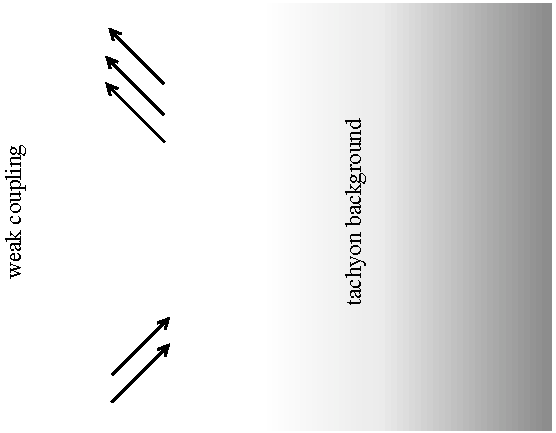
\includegraphics[width=0.73\linewidth]{figures/fig_9_12.pdf}
\caption{ディラトン背景とタキオン背景をもつ時空。相互作用の強さは右へ進むほど増えるが、タキオン背景からの有効ポテンシャルによって遮られる。}
\label{fig:9.12}
\end{figure}

$D>2$ では、タキオン背景の物理的な効果はそれほど明らかでないが、この場合にも障壁として働くと論じられてきた。しかし、別の理由から $D\leq2$ が中心に研究されてきた。これらの理論は、実際に解けるのである。まず、弦を量子化すると、ゲージ対称性が二組の振動子を取り除くので、$D\leq2$ では何も残らないことに注目しよう。残るのは重心運動、すなわち単一のスカラーだけである。\footnote[5]{特別な運動量では、追加の物理的状態が見いだされる。これらは弦の場の理論の破れていない対称性と解釈でき、おそらく理論の可解性に役割を果たしている。}
それでも、弦理論を直接解くのはなおかなり難しい。まず、作用 (9.9.5) をもつ世界面の経路積分を評価しなければならない。指数関数的なタキオン場のため、これはもはや自由理論ではない。これは \textbf{Liouville 場の理論}として知られる。古典的には可積分であり、大きな努力によっていくつかの量子振幅も求められている。しかし弦理論を解くには、さらに各種数で得られた結果を、Riemann 面のモジュライ空間にわたって積分する必要がある。この空間が複雑であることは、すでに見た。驚くべきことに、まったく異なる方法によって、あらゆる次数の完全な振幅が求められている。これを説明するには、まず別の考えを導入しなければならない。

\subsubsectionlink*{非臨界弦}

$d$ 次元 Euclid 空間内の2次元曲面についての和で定義される、統計力学系を考えよう。さらに曲面には、長さの尺度と解釈できる何らかの内部自由度があるとする。系を記述する自然な場は、埋め込み $X^\mu(\sigma)$ と計量 $g_{ab}(\sigma)$ である。しかし、長さが問題から消える、すなわち理論が Weyl 不変になる特別な理由はない。そのため、これは\textbf{非臨界弦}と呼ばれる。この系の最も低い次元の作用、あるいは統計力学の文脈で経路積分を考えているので Boltzmann の重みは、Polyakov 作用に、世界面の宇宙項を加えたものとなる。臨界弦では、この項は Weyl 不変性によって禁じられる。
\begin{equation}
S=\frac1{4\pi\alpha'}\int_M d^2\sigma\,g^{1/2}
\left(g^{ab}\partial_aX^\mu\partial_bX_\mu+\mu\right).
\tag{9.9.6}\label{eq:9.9.6}
\end{equation}

Weyl 不変性がなくても、微分同相不変性を用いて計量を部分的に固定できるが、一つの自由度が残る。
\begin{equation}
g_{ab}(\sigma)=\exp(2\phi(\sigma))\widehat g_{ab}(\sigma).
\tag{9.9.7}\label{eq:9.9.7}
\end{equation}
$\widehat g_{ab}$ はゲージの選択であり、計量のスケール $\phi$ は依然として経路積分される。このゲージ固定の Faddeev--Popov 行列式は、式 (3.4.19) と同じである。後者における Weyl ゲージ固定の寄与は自明だからである。曲率が
\begin{equation}
g^{1/2}R=\widehat g^{1/2}
\left(\widehat R-2\widehat\nabla^2\phi\right)
\tag{9.9.8}\label{eq:9.9.8}
\end{equation}
となる計量 (9.9.7) を代入し、場に依存しない項を省くと、作用と Faddeev--Popov 行列式を合わせたものは
\begin{equation}
\begin{split}
S=\frac1{4\pi\alpha'}\int_M d^2\sigma\,\widehat g^{1/2}
\biggl[&
\widehat g^{ab}\partial_aX^\mu\partial_bX_\mu+\mu\exp2\phi\\
&+\frac{13\alpha'}3
\left(\widehat g^{ab}\partial_a\phi\partial_b\phi+\widehat R\phi\right)
\biggr]
\end{split}
\tag{9.9.9}\label{eq:9.9.9}
\end{equation}
となる。Faddeev--Popov 行列式が $\phi$ の運動項を与えたことに注意しよう。これをディラトン・タキオン作用 (9.9.5) と比べると、著しく似ている。$d=D-1$ とし、新しい場 $\phi$ を $x^1$ と解釈し、作用 (9.9.5) では完全にゲージ固定できるので $g_{ab}\to\widehat g_{ab}$ と名前を変えると、同じ項がすべて現れる。いくつかの係数は少し異なり、すべてを一致させる $\phi$ のスケール変換は存在しない。それでも、実際にはこれらは同じ場の理論であると主張する。要点は、臨界弦の経路積分 (9.9.5) は $\widehat g_{ab}$ を計量として定義され、非臨界弦 (9.9.9) は $\exp(2\phi)\widehat g_{ab}$ を用いて定義されることである。測度の Weyl 変換を注意深く扱えば、一方から他方へ変換される。非臨界弦の定義には完全な計量 (9.9.7) だけが現れるので、
\begin{align}
\widehat g_{ab}(\sigma)&\longrightarrow
\exp(2\omega(\sigma))\widehat g_{ab}(\sigma),
\tag{9.9.10a}\label{eq:9.9.10a}\\
\phi(\sigma)&\longrightarrow\phi(\sigma)-\omega(\sigma)
\tag{9.9.10b}\label{eq:9.9.10b}
\end{align}
によって何も変わりえないことに注目すれば、これは容易に理解できる。こうして非臨界弦は Weyl 不変性を獲得し、それだけで自由パラメーター $\mu$ を除くさまざまな係数が決まる。

Weyl 不変な理論と不変でない理論が等価になれるのは、奇妙に思えるかもしれない。要点は、場の理論では、ゲージ固定だけに使う余分な場も加えれば、余分な「見かけだけの」ゲージ対称性をいつでも加えられることである。結局、ゲージ対称性は記述の冗長性にすぎず、いつでも、より冗長な記述を採用できる。対称性 (9.9.10) では、Weyl 対称性と場 $\phi$ を単に相殺できるのは明らかである。しかし一般の弦背景、例えば埋め込み座標が Weyl 不変な平坦空間では、これは不可能であり、Weyl 不変性は「本物」である。

いずれにせよ、いよいよ要点に近づいた。非臨界弦は、三角形分割された曲面についての和で近似でき、二点の間の辺の数を長さの尺度とする。これらの三角形分割された曲面は大きな Feynman 図に似ており、実際、これを図式展開としてもつ量子系、すなわち\textbf{行列模型}が見つかる。行列模型の場は $N\times N$ 行列である。$N\to\infty$ とし、他の結合を調整すると、少なくとも $D\leq2$ では、大きく滑らかな曲面が支配的な臨界点があり、非臨界弦が回復される。さらに、行列模型は、やはり $D\leq2$ で、行列を対角化することで解ける。最終的に得られるのは、固有値の空間を運動する相互作用しないフェルミオンという、かなり単純な系である。そして上の手順をたどり直せば、すべての種数の弦振幅を計算できる。

これらの方法は本書の他の部分から大きく離れるので、詳細は参考文献に委ねなければならない。いずれにせよ、$D>2$ や超対称理論では、まだ有用なものにはなっていない。ただし第14章で見るように、多少異なる大 $N$ 行列の理論が、非摂動的弦理論として最近提案された。しかし、これらの模型から得られた重要な教訓を、少なくとも一つは挙げておくべきだろう。それは摂動論の $(2g)!$ の振る舞いである。これは、行列模型の明示的な解で初めて見られ、その後すべての弦理論で成り立つと論じられた。行列模型では、対応する $\exp[O(-1/g_{\mathrm c})]$ の効果は、固有値の空間でのフェルミオンのトンネル効果に関係する。これが、より高次元の弦理論の $\exp[O(-1/g_{\mathrm c})]$ の効果と関係付けられるかどうかは明らかでない。

\subsectionlink*{演習問題}
\addcontentsline{toc}{subsection}{演習問題}

\subsubsectionlink*{演習9.1}\label{ex:9.1}
(a) 共形変換を用いて、OPE (9.1.2) と期待値 (9.1.3) から内積 (9.1.29) が従うことを示せ。

(b) 基底 $|\widehat{\mathcal V}_j(k)\rangle$ で行列要素を取り、式 (9.1.28) の第二の等号を確認せよ。

\subsubsectionlink*{演習9.2}\label{ex:9.2}
(a) 球面に対する式 (9.1.17) と同様に、ただし今度はトレースを含む形で、トーラス上の4点振幅を演算子形式で書け。

(b) 頂点演算子の一つがヌル、すなわち $\widehat{\mathcal V}_1=\{Q_{\mathrm B},\mathcal X\}$ なら、トレースが、頂点演算子の位置に関する全微分と、$\tau,\bar\tau$ に関する全微分の和に等しいことを示せ。

\subsubsectionlink*{演習9.3}\label{ex:9.3}
(a) 四つの頂点演算子をもつトーラスに対し、前問 (a) の結果を用い、$w_1,w_2,w_3-w_4$ を固定し、$w_3$ と $2\pi\tau-w_3$ が $i\infty$ に近づく極限でのユニタリティを調べよ。これは二つのハンドルが退化する極限であり、ユニタリティはその振幅を、二つの木レベル4点振幅の積に関係付ける。

(b) 特に、全 Hilbert 空間 $\widehat{\mathcal H}$ にわたる和と、物理的 Hilbert 空間にわたる和が等しいという証明を繰り返せ。そのためには、異なるゴースト数をもつ中間状態の間の相殺が必要なことを示せ。この相殺は、ゲージ理論での Faddeev--Popov ゴーストと縦偏極ゲージボソンの相殺を、弦へ一般化したものである。

\subsubsectionlink*{演習9.4}\label{ex:9.4}
図9.6(a)の Feynman グラフが覆う領域についての、式 (9.3.7) の主張を確認し、このグラフが覆う他の二つの領域を求めよ。

\subsubsectionlink*{演習9.5}\label{ex:9.5}
(a) 弦の場の展開の項 (9.6.7) について、ゲージ変換 (9.6.2) と作用 (9.6.3) を明示的に書き下せ。

(b) 補助場と、ゲージ変換で完全に取り除ける場を消去し、得られる $A_\mu$ のゲージ変換と作用が期待される形をもつことを示せ。

\subsubsectionlink*{演習9.6}\label{ex:9.6}
$f_{2k}=k^ab^k$ に対し、級数 (9.7.5) の最小項が $\exp(-C/g^2)$ の程度であることを示せ。$C$ を求めるのに十分な精度で計算せよ。級数 (9.7.2) について、インスタントン作用と比較せよ。

\subsubsectionlink*{演習9.7}\label{ex:9.7}
量子論では、Euclid 時間の周期が $T^{-1}$ の Euclid 経路積分は、熱分配関数 $\exp[-\widetilde F(T)/T]$ を与える。弦の経路積分について、これが結果 (9.8.15) と一致することを示せ。唯一の微妙な点は、積分領域と巻き付き数についての和との関係である。（参考文献：McClain \& Roth (1987)\cite{McClain:1986id}。）

\subsubsectionlink*{演習9.8}\label{ex:9.8}
線形ディラトン背景 (9.9.1) におけるタキオンの波動方程式 (9.9.2) に対し、$D\leq2$ なら、任意の\textbf{有限エネルギー}の初期配置が、安定な、すなわち振動的な時間発展をすることを示せ。

\subsubsectionlink*{演習9.9}\label{ex:9.9}
$D=2$ の線形ディラトン背景における閉弦の重力子レベルについて、物理的状態条件を OCQ または BRST の形式で調べよ。運動量には複素数値を許せ。一般の運動量では物理的スペクトルは自明だが、二つの運動量では非自明な物理的状態があるはずである。

\subsubsectionlink*{演習9.10}\label{ex:9.10}
式 (9.8.14) を導け。ヒント：第二行で、$m^2$ が $m^2+\boldsymbol k^2$ になるように $\boldsymbol k$ の積分を導入する。次に $t$ を積分する。結果は初等関数で表される。最後に、$r$ の和は第一行の対数の級数展開である。

\clearpage
\appendix
\renewcommand{\thefigure}{\Alph{section}.\arabic{figure}}
\sectionlink{経路積分の短期講義}\label{app:A}

経路積分は、特に非自明な位相を持つ曲面上で、量子論を表す強力な手段である。ここで示す入門は、現代の場の理論の教科書で読者が目にするものと同様である。経路積分と Hilbert 空間形式の関係や、経路積分内での演算子方程式の使用など、必要となるいくつかの考え方を強調するために、本付録を設けた。

\subsectionlink{ボソン場}

まず、一自由度で Hamiltonian $\hat H(\hat p,\hat q)$ を持つ量子力学の問題を考える。ここで
\begin{equation}
[\hat q,\hat p]=i\hbar.
\tag{A.1.1}\label{eq:A.1.1}
\end{equation}
本付録では一貫して、ハットで演算子を表す。関心のある基本的な量は、時間 $T$ の間に、ある $q$ 固有状態から別の固有状態へ発展する振幅
\begin{equation}
\langle q_f|\exp(-i\hat HT/\hbar)|q_i\rangle
\tag{A.1.2}\label{eq:A.1.2}
\end{equation}
である。

場の理論では、一般に Heisenberg 表示を使うと便利である。この表示で演算子の時間依存性は
\begin{equation}
\hat A(t)=\exp(i\hat Ht/\hbar)\hat A\exp(-i\hat Ht/\hbar)
\tag{A.1.3}\label{eq:A.1.3}
\end{equation}
である。状態 $\lvert q,t\rangle$ は $\hat q(t)$ の固有状態であり、
\begin{equation}
\hat q(t)|q,t\rangle=|q,t\rangle q.
\tag{A.1.4}\label{eq:A.1.4}
\end{equation}
$t=0$ の Schrödinger 固有状態で書けば、
\begin{equation}
|q,t\rangle=\exp(i\hat Ht/\hbar)|q\rangle.
\tag{A.1.5}\label{eq:A.1.5}
\end{equation}
この記法では、遷移振幅\hyperref[eq:A.1.2]{(A.1.2)}は $\langle q_f,T|q_i,0\rangle$ である。

\begin{figure}[tbp]
\centering
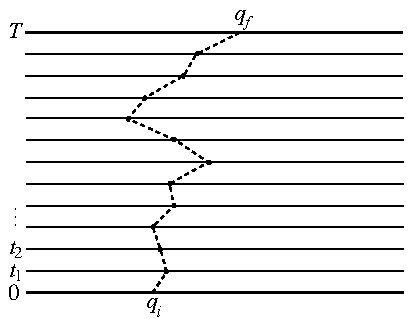
\includegraphics[width=0.8\linewidth]{figures/fig_A_1.pdf}
\caption{時間刻みに分解した遷移振幅。破線は区分的に線形な経路を示唆しており、これは経路積分を定義する多くの方法の一つである。}
\label{fig:A.1}
\end{figure}

状態の完全系を挿入すると、遷移振幅を、中間のある時刻 $t$ に系が通過しうるすべての状態 $q$ にわたる、コヒーレントな和として書ける。
\begin{equation}
\langle q_f,T|q_i,0\rangle
=\int dq\,\langle q_f,T|q,t\rangle\langle q,t|q_i,0\rangle.
\tag{A.1.6}\label{eq:A.1.6}
\end{equation}
図\ref{fig:A.1}のように時間区間をさらに $N$ 個の刻みに分け、
\begin{equation}
t_m=m\epsilon,\qquad\epsilon=T/N
\tag{A.1.7}\label{eq:A.1.7}
\end{equation}
とし、各中間時刻に対応して状態の完全系を挿入する。
\begin{equation}
\langle q_f,T|q_i,0\rangle
=\int dq_{N-1}\cdots dq_1
\prod_{m=0}^{N-1}\langle q_{m+1},t_{m+1}|q_m,t_m\rangle.
\tag{A.1.8}\label{eq:A.1.8}
\end{equation}
Schrödinger 形式に戻し、中間の運動量についての積分を導入する。
\begin{equation}
\begin{aligned}
\langle q_{m+1},t_{m+1}|q_m,t_m\rangle
&=\langle q_{m+1}|\exp(-i\hat H\epsilon/\hbar)|q_m\rangle\\
&=\int dp_m\,\langle q_{m+1}|p_m\rangle
\langle p_m|\exp(-i\hat H\epsilon/\hbar)|q_m\rangle.
\end{aligned}
\tag{A.1.9}\label{eq:A.1.9}
\end{equation}
交換関係を用いれば、$\hat H$ は常に、すべての $\hat p$ を左、すべての $\hat q$ を右に置いて書けるので、
\begin{equation}
\langle p_m|\hat H(\hat p,\hat q)|q_m\rangle
=H(p_m,q_m)\langle p_m|q_m\rangle.
\tag{A.1.10}\label{eq:A.1.10}
\end{equation}
これを用いて式\hyperref[eq:A.1.9]{(A.1.9)}の行列要素を評価する。指数関数を展開すると、$\hat q$ が $\hat p$ の左にある $\epsilon^2$ 以上の次数の項が生じるが、これらを捨てる。この次数までで、$\langle q_{m+1},t_{m+1}|q_m,t_m\rangle$ は
\begin{equation}
\begin{aligned}
&\int dp_m\,\exp[-iH(p_m,q_m)\epsilon/\hbar]
\langle q_{m+1}|p_m\rangle\langle p_m|q_m\rangle\\
&\quad=\int\frac{dp_m}{2\pi\hbar}
\exp\left\{-\frac i\hbar
[H(p_m,q_m)\epsilon-p_m(q_{m+1}-q_m)]
+O(\epsilon^2)\right\}
\end{aligned}
\tag{A.1.11}\label{eq:A.1.11}
\end{equation}
となる。したがって、
\begin{equation}
\begin{aligned}
\langle q_f,T|q_i,0\rangle
\approx{}&\int\frac{dp_{N-1}}{2\pi\hbar}\,dq_{N-1}\cdots
\frac{dp_1}{2\pi\hbar}\,dq_1\frac{dp_0}{2\pi\hbar}\\
&\times\exp\left\{-\frac i\hbar
\sum_{m=0}^{N-1}
[H(p_m,q_m)\epsilon-p_m(q_{m+1}-q_m)]\right\}\\
\longrightarrow{}&\int[dp\,dq]\,
\exp\left\{\frac i\hbar\int_0^Tdt\,[p\dot q-H(p,q)]\right\}.
\end{aligned}
\tag{A.1.12}\label{eq:A.1.12}
\end{equation}
最終行では形式的な $\epsilon\to0$ の極限をとったので、積分は、指定した $q(T)$ と $q(0)$ を持つすべての経路 $p(t),q(t)$ にわたる。これは Hamiltonian 経路積分（または汎関数積分）であり、Hamiltonian 形式の作用を $S$ として、$\exp(iS/\hbar)$ で重みを付けた位相空間の経路についての和である。

$p(t)$ について積分しよう。まず、積分は位相が停留する点によって支配されると近似する。
\begin{equation}
0=\frac{\partial}{\partial p}[p\dot q-H(p,q)]
=\dot q-\frac{\partial}{\partial p}H(p,q).
\tag{A.1.13}\label{eq:A.1.13}
\end{equation}
$p$ を $q,\dot q$ で解き、$L=p\dot q-H$ を思い出すと、停留位相近似は
\begin{equation}
\langle q_f,T|q_i,0\rangle
=\int[dq]\exp\left[\frac i\hbar\int_0^Tdt\,L(q,\dot q)\right]
\tag{A.1.14}\label{eq:A.1.14}
\end{equation}
を与える。しばしば運動量積分は Gaussian 型で、$\hat H=\tfrac12\hat p^2+V(\hat q)$ であり、その場合には、測度 $[dq]$ に吸収できる規格化を除き、停留位相近似は厳密である。実際、一般にも同じことができる。$p$ と $\dot q$ の関係\hyperref[eq:A.1.13]{(A.1.13)}が局所的なので、停留位相近似への補正も局所的であり、$[dq]$ が各中間時刻での独立した積分の積であるという本質的な性質を損なわずに、その定義に吸収できるからである。結果\hyperref[eq:A.1.14]{(A.1.14)}は Lagrangian 経路積分である。これは、今度は Lagrangian 形式の作用を $S$ として、$\exp(iS/\hbar)$ で重みを付けた配位空間のすべての経路についての積分である。

古典極限を議論するために $\hbar$ を残しておいた。$\hbar\to0$ では、位相が停留する経路、$\delta S/\delta q(t)=0$ が積分を支配する。これは確かに古典的な運動方程式である。以後は $\hbar=1$ とする。

以上の導出は、明らかに多成分の $q^i$ に一般化できる。空間座標 $\mathbf x$ を離散化して極限をとるか、$\mathbf x$ 依存性を Fourier モードで展開すれば、場の量子論は常に無限個の $q$ で書ける。したがって、上の経路積分表示の導出は、ボソン場の理論にも適用できる。

経路積分の公式の導出では、連続極限 $\epsilon\to0$ をかなり発見的に扱った。繰り込み理論は、この極限操作を研究するものであり、かなりよく理解されている。Lagrangian が一定の条件（繰り込み可能性）を満たし、極限をとる際に Lagrangian の係数（裸の結合定数）を適切に変化させれば、極限は存在する。結果は、途中で選ばなければならないさまざまな事柄、たとえば Hamiltonian 内の演算子の順序、測度の厳密な定義、正則化の違い（たとえば図で示唆した区分的線形経路の極限と、Fourier モードの周波数カットオフとの違い）に依存しない。\footnote[1]{別の例として、場のスケールを自由に変えてよい。その Jacobian は形式的には各点での Jacobian の積であり、その対数は各点での局所的な式の和になる。正則化すると、これは裸の結合定数の移動にすぎない。}これらは局所的な効果なので、すべて裸の結合定数に吸収できる。実際に明示的に評価するのは、少数の Gaussian 経路積分だけである。経路積分は主として、演算子方程式や縫い合わせの関係など、一般的な結果を導くために用いる。

\subsubsectionlink*{Hilbert 空間形式との関係}

経路積分から出発し、それを切り開くことで、理論の Hilbert 空間を回復できる。式\hyperref[eq:A.1.6]{(A.1.6)}で、各振幅を経路積分として書くと、
\begin{equation}
\begin{aligned}
&\int[dq]_{q_i,0}^{q_f,T}
\exp\left(i\int_0^Tdt\,L\right)\\
&\quad=\int dq\int[dq]_{q,t}^{q_f,T}
\exp\left(i\int_t^Tdt\,L\right)
\int[dq]_{q_i,0}^{q,t}
\exp\left(i\int_0^tdt\,L\right).
\end{aligned}
\tag{A.1.15}\label{eq:A.1.15}
\end{equation}
すなわち、$[0,T]$ 上の経路積分は、$[0,t]$ と $[t,T]$ 上の別々の経路積分と、$q(t)$ に関する通常の積分とに分かれる。経路の境界条件は上下の添字で示した。$T\geq t\geq0$ という制限に注意しよう。中間の積分は、任意の完全な状態系についての和に置き換えてもよい。この切断（逆にいえば縫い合わせ）の原理は、弦理論に現れる非自明な位相の曲面で特に有用である。そのような曲面は、さまざまな閉曲線に沿って切り開ける。異なる選び方は、一つの振幅に対して異なる Hilbert 空間表示を与える。これは世界面双対性として知られている。

ここで、$0<t<T$ において因子 $q(t)$ を追加で挿入した経路積分を考えよう。切断関係\hyperref[eq:A.1.15]{(A.1.15)}を用いると、
\begin{equation}
\begin{aligned}
\int[dq]_{q_i,0}^{q_f,T}\exp(iS)q(t)
&=\int dq\,\langle q_f,T|q,t\rangle\,q\,\langle q,t|q_i,0\rangle\\
&=\int dq\,\langle q_f,T|\hat q(t)|q,t\rangle
\langle q,t|q_i,0\rangle\\
&=\langle q_f,T|\hat q(t)|q_i,0\rangle.
\end{aligned}
\tag{A.1.16}\label{eq:A.1.16}
\end{equation}
したがって、汎関数積分の $q(t)$ は、行列要素の $\hat q(t)$ に翻訳される。二つの挿入の積 $q(t)q(t')$（単なる積分変数なので $q(t')q(t)$ と等しい）について、$t,t'$ がともに $[0,T]$ にあるとすると、同じ方法で
\begin{equation}
\int[dq]_{q_i,0}^{q_f,T}\exp(iS)q(t)q(t')
=\langle q_f,T|\mathrm T[\hat q(t)\hat q(t')]|q_i,0\rangle
\tag{A.1.17}\label{eq:A.1.17}
\end{equation}
が得られる。ここで $\mathrm T$ は時間順序積
\begin{equation}
\mathrm T[\hat A(t)\hat B(t')]
=\theta(t-t')\hat A(t)\hat B(t')
+\theta(t'-t)\hat B(t')\hat A(t)
\tag{A.1.18}\label{eq:A.1.18}
\end{equation}
を表す。経路積分は無限小の時間切片を順次つないで構成されるため、経路積分中の二つ以上の挿入は、常に行列要素中の演算子の時間順序積に対応する。

運動方程式は $\delta S/\delta q(t)=0$ である。これが経路積分の中でどのように働くかを見よう。他の挿入 $\mathcal F$ を伴う経路積分で、この方程式を考える。
\begin{equation}
\begin{aligned}
\int[dq]_{q_i,0}^{q_f,T}\exp(iS)\frac{\delta S}{\delta q(t)}\mathcal F
&=-i\int[dq]_{q_i,0}^{q_f,T}
\left[\frac{\delta}{\delta q(t)}\exp(iS)\right]\mathcal F\\
&=i\int[dq]_{q_i,0}^{q_f,T}\exp(iS)
\frac{\delta\mathcal F}{\delta q(t)}.
\end{aligned}
\tag{A.1.19}\label{eq:A.1.19}
\end{equation}
第二行では部分積分した。\footnote[2]{汎関数微分は
\[
\frac{\delta}{\delta q(t)}q(t')=\delta(t-t')
\]
と定義される。これは通常の微分
\[
\frac1\epsilon\frac{\partial}{\partial q_m},
\qquad m=t/\epsilon
\]
の極限とみなせる。特に、通常の微分と同様に、汎関数微分を部分積分できる。}
$\mathcal F$ の中の場がどれも時刻 $t$ にない場合、右辺は消え、運動方程式は経路積分内で成立する。そこで、運動方程式は演算子方程式として成り立つという。これは今後広く用いる手法である。演算子方程式とは、その方程式に含まれる場と位置が一致する他の場を持たない、任意の経路積分に挿入したときに成立する方程式である。Hilbert 空間の言葉に翻訳すると、他の挿入 $\mathcal F$ によって任意の初期状態と終状態を設定できるので、これは、演算子方程式は一般の行列要素に対して成り立つはずだという通常の概念に対応する。

時刻 $t$ に追加の挿入が存在すると、経路積分内の演算子方程式は、デルタ関数の源の項を追加した形でのみ成立する。たとえば $\mathcal F=q(t')\cdots$ とし、$t'$ は $t$ の近く、「$\cdots$」の他の場は遠くにあるとしよう。式\hyperref[eq:A.1.19]{(A.1.19)}は
\begin{equation}
\left\langle q(t')\frac{\delta S}{\delta q(t)}\cdots\right\rangle
=i\langle\delta(t-t')\cdots\rangle
\tag{A.1.20}\label{eq:A.1.20}
\end{equation}
となる。これは、場の積の期待値についての運動方程式である Schwinger--Dyson 方程式の例である。同じ結果を演算子方程式として書けば、
\begin{equation}
q(t')\frac{\delta S}{\delta q(t)}=i\delta(t-t').
\tag{A.1.21}\label{eq:A.1.21}
\end{equation}

具体例として、調和振動子をとる。
\begin{align}
S&=\frac12\int dt\,(\dot q^2-\omega^2q^2),
\tag{A.1.22a}\label{eq:A.1.22a}\\
\frac{\delta S}{\delta q(t)}&=-\ddot q(t)-\omega^2q(t).
\tag{A.1.22b}\label{eq:A.1.22b}
\end{align}
導いた演算子方程式は
\begin{equation}
\left(\frac{\partial^2}{\partial t^2}+\omega^2\right)q(t)=0
\tag{A.1.23}\label{eq:A.1.23}
\end{equation}
および
\begin{equation}
\left(\frac{\partial^2}{\partial t^2}+\omega^2\right)
q(t)q(t')=-i\delta(t-t')
\tag{A.1.24}\label{eq:A.1.24}
\end{equation}
である。Hilbert 空間の言葉では、これらは
\begin{equation}
\begin{aligned}
\left(\frac{\partial^2}{\partial t^2}+\omega^2\right)\hat q(t)&=0,\\
\left(\frac{\partial^2}{\partial t^2}+\omega^2\right)
\mathrm T[\hat q(t)\hat q(t')]&=-i\delta(t-t')
\end{aligned}
\tag{A.1.25a}\label{eq:A.1.25a}
\end{equation}
となる。第一式は場の演算子の Heisenberg 方程式であり、第二式のデルタ関数は、時間順序積の階段関数に時間微分が作用することから生じる。
\begin{equation}
\begin{aligned}
\left(\frac{\partial^2}{\partial t^2}+\omega^2\right)
\mathrm T[\hat q(t)\hat q(t')]
={}&\mathrm T\left\{[\ddot{\hat q}(t)+\omega^2\hat q(t)]\hat q(t')\right\}\\
&+\delta(t-t')[\dot{\hat q}(t),\hat q(t)]\\
={}&0-i\delta(t-t').
\end{aligned}
\tag{A.1.26}\label{eq:A.1.26}
\end{equation}

\subsubsectionlink*{Euclid 経路積分}

Schrödinger の言葉では、時間順序積\hyperref[eq:A.1.17]{(A.1.17)}は
\begin{equation}
\langle q_f|
\exp[-i\hat H(T-t_>)]\hat q\,
\exp[-i\hat H(t_>-t_<)]\hat q\,
\exp[-i\hat Ht_<]|q_i\rangle
\tag{A.1.27}\label{eq:A.1.27}
\end{equation}
である。$t_>$ は $t,t'$ の大きい方、$t_<$ は小さい方である。時間刻みを順次つないで振幅を作るという経路積分の性質により、\hyperref[eq:A.1.27]{(A.1.27)}のような振幅で $H$ に掛かる時間差は常に正である。すなわち、$\exp(-iH\Delta t)$ に現れるのは正の $\Delta t$ だけである。ここで、すべての時間を複素平面で一様に回転し、$0\leq\theta\leq\pi$ の任意の位相について $t\to e^{-i\theta}t$ として解析接続する。指数の実部は $-E\sin\theta\,\Delta t$ であり、$E$ は中間状態のエネルギーである。安定な系では Hamiltonian は下に有界なので、中間状態についての和は問題なく収束し、特異点には遭遇しない。接続された振幅は明確に定義される。

実数 $u$ に対して $t=-iu$ と時間を純虚数にとると、これまで調べた Minkowski 振幅に対する Euclid 振幅が定義される。
\begin{equation}
\left\langle q_f,u\left|
\mathrm T\left[\prod_a\hat q(u_a)\right]\right|q_i,0\right\rangle_{\mathrm E}
\tag{A.1.28}\label{eq:A.1.28}
\end{equation}
は、
\begin{equation}
\left\langle q_f,t\left|
\mathrm T\left[\prod_a\hat q(t_a)\right]\right|q_i,0\right\rangle
\tag{A.1.29}\label{eq:A.1.29}
\end{equation}
を $t=-iu$ へ接続したものとして定義する。Euclid の場合にも経路積分表示の導出を繰り返せるが、結果はきわめて簡単であり、作用中の $t$ を $-iu$ に置き換えるだけである。
\begin{equation}
\begin{aligned}
&\left\langle q_f,U\left|
\mathrm T\left[\prod_a\hat q(u_a)\right]\right|q_i,0\right\rangle_{\mathrm E}\\
&\qquad=\int[dq]_{q_i,0}^{q_f,U}
\exp\left[\int_0^Udu\,L(q,i\partial_uq)\right]\prod_aq(u_a).
\end{aligned}
\tag{A.1.30}\label{eq:A.1.30}
\end{equation}
Euclid 経路積分の重みは、慣習的に $\exp(-S_{\mathrm E})$ と定義するので、Euclid 作用には負号が入る。
\begin{equation}
S_{\mathrm E}=\int du\,L_{\mathrm E}(q,\partial_uq)
=-\int du\,L(q,i\partial_uq).
\tag{A.1.31}\label{eq:A.1.31}
\end{equation}
作用の指数関数が振動せずに減衰するため、Euclid 経路積分の方が通常は明確に定義される。その後、解析接続によって Minkowski の行列要素が得られる。本書の本文で主に扱うのは Euclid 経路積分であり、弦の S 行列を表すために用いる。

しばしば関心があるのは、たとえば
\begin{equation}
\operatorname{Tr}\exp(-\hat HU)=\sum_i\exp(-E_iU)
\tag{A.1.32}\label{eq:A.1.32}
\end{equation}
のようなトレースである。和は $\hat H$ のすべての固有ベクトルにわたり、$E_i$ は対応する固有値である。$q$ 基底ではトレースは
\begin{equation}
\begin{aligned}
\int dq\,\langle q|\exp(-\hat HU)|q\rangle
&=\int dq\,\langle q,U|q,0\rangle_{\mathrm E}\\
&=\int dq\int[dq]_{q,0}^{q,U}\exp(-S_{\mathrm E})\\
&=\int[dq]_{\mathrm P}\exp(-S_{\mathrm E})
\end{aligned}
\tag{A.1.33}\label{eq:A.1.33}
\end{equation}
となる。最終行の $[dq]_{\mathrm P}$ は、$[0,U]$ 上のすべての周期的な経路についての積分を表す。興味深い変形として、すべての反周期的な経路についての積分がある。
\begin{equation}
\begin{aligned}
\int[dq]_{\mathrm A}\exp(-S_{\mathrm E})
&=\int dq\int[dq]_{-q,0}^{q,U}\exp(-S_{\mathrm E})\\
&=\int dq\,\langle q,U|-q,0\rangle_{\mathrm E}\\
&=\int dq\,\langle q,U|\hat R|q,0\rangle_{\mathrm E}\\
&=\operatorname{Tr}[\exp(-\hat HU)\hat R].
\end{aligned}
\tag{A.1.34}\label{eq:A.1.34}
\end{equation}
ここで $\hat R$ は $q$ を $-q$ にする反射演算子である。境界条件をひねること、たとえば周期的なものを反周期的なものに置き換えることは、トレース内に演算子を挿入することに等しいとわかる。$\hat R^2=1$ なので、固有値は $\pm1$ である。周期的な経路積分と反周期的な経路積分の平均をとると、$\hat R=+1$ の空間に射影する $\tfrac12(1+\hat R)$ が挿入される。
\begin{equation}
\frac12(\text{周期的}+\text{反周期的})
=\sum_{R_i=+1}\exp(-E_iU).
\tag{A.1.35}\label{eq:A.1.35}
\end{equation}
同様に、$\tfrac12(\text{周期的}-\text{反周期的})$ は $\hat R=-1$ の空間上のトレースを与える。

小さいが、ときに混乱を招く点がある。$\hat A$ が Hermite 演算子であっても、Euclid の Heisenberg 演算子 $\hat A(u)=\exp(\hat Hu)\hat A\exp(-\hat Hu)$ は
\begin{equation}
\hat A(u)^\dagger=\hat A(-u)
\tag{A.1.36}\label{eq:A.1.36}
\end{equation}
を満たすため、一般には Hermite ではない。このため、Euclid 随伴
\begin{equation}
\overline{\hat A(u)}=\hat A(-u)^\dagger
\tag{A.1.37}\label{eq:A.1.37}
\end{equation}
を定義すると便利である。Schrödinger 描像の Hermite 演算子は、Euclid の Heisenberg 描像では Euclid 自己随伴になる。

\subsubsectionlink*{図式と行列式}

図式展開は、経路積分から容易に得られる。この話題は現代の場の理論の教科書でよく扱われている。ここでは、本文で使ういくつかの結果だけを導く。記法を明確にするために場の理論へ移り、$q(t)$ を実スカラー場 $\phi(t,\mathbf x)$ に置き換える。自由な作用
\begin{equation}
\frac12\int d^dx\,\phi(x)\Delta\phi(x)
\tag{A.1.38}\label{eq:A.1.38}
\end{equation}
から出発する。ここで $\Delta$ はある微分演算子である。具体的に Euclid の場合をとり、源 $J(x)$ を持つ経路積分を考える。
\begin{equation}
\begin{aligned}
Z[J]&=\left\langle\exp\left[i\int d^dx\,J(x)\phi(x)\right]\right\rangle\\
&=\int[d\phi]\exp\left[
-\frac12\int d^dx\,\phi(x)\Delta\phi(x)
+i\int d^dx\,J(x)\phi(x)\right].
\end{aligned}
\tag{A.1.39}\label{eq:A.1.39}
\end{equation}
これは Euclid の Green 関数の生成汎関数である。$J(x)$ に関する汎関数微分をとると、積分内に因子 $i\phi(x)$ が降りてくる。$\phi$ を $\phi+i\Delta^{-1}J$ にずらすと平方完成され、
\begin{equation}
\begin{aligned}
Z[J]&=Z[0]\exp\left[
-\frac12\int d^dx\,d^dy\,J(x)\Delta^{-1}(x,y)J(y)\right]\\
&=Z[0]\exp\left[
\frac12\int d^dx\,d^dy\,\Delta^{-1}(x,y)
\frac{\delta^2}{\delta\phi(x)\delta\phi(y)}\right]\\
&\qquad\times
\left.\exp\left[i\int d^dx\,J(x)\phi(x)\right]\right|_{\phi=0}
\end{aligned}
\tag{A.1.40}\label{eq:A.1.40}
\end{equation}
が残る。第二行では、各 $\phi$ 微分が $iJ$ になる。$\phi$ の任意の汎関数 $\mathcal F$ は
\begin{equation}
\mathcal F[\phi]
=\int[dJ]\exp\left[i\int d^dx\,J(x)\phi(x)\right]f[J]
\tag{A.1.41}\label{eq:A.1.41}
\end{equation}
と書ける。$f[J]$ は $\mathcal F$ の（汎関数の）Fourier 変換である。線形性から
\begin{equation}
\langle\mathcal F\rangle
=Z[0]\left.
\exp\left[
\frac12\int d^dx\,d^dy\,\Delta^{-1}(x,y)
\frac{\delta^2}{\delta\phi(x)\delta\phi(y)}\right]\mathcal F[\phi]
\right|_{\phi=0}
\tag{A.1.42}\label{eq:A.1.42}
\end{equation}
が得られる。指数関数を展開すると、$\mathcal F$ 内の場の対を縮約するすべての方法、すなわち図式展開が生成される。また、$\mathcal F$ が因子の積 $\mathcal F_1\mathcal F_2\cdots$ であるとき、
\begin{equation}
\frac{\delta}{\delta\phi(x)}
=\frac{\delta}{\delta\phi_1(x)}
+\frac{\delta}{\delta\phi_2(x)}+\cdots
\tag{A.1.43}\label{eq:A.1.43}
\end{equation}
と分けられる。ここで $\delta/\delta\phi_i$ は $\mathcal F_i$ にだけ作用する。自己縮約は、項
\begin{equation}
\frac{\delta^2}{\delta\phi_i(x)\delta\phi_i(y)}
\qquad(i\text{ について和をとらない})
\tag{A.1.44}\label{eq:A.1.44}
\end{equation}
である。

次に全体の因子 $Z[0]$ を考える。$\Delta$ は自己随伴と仮定し、その固有関数 $\Phi_i(x)$ の完全系で $\phi(x)$ を展開する。
\begin{equation}
\phi(x)=\sum_i\phi_i\Phi_i(x).
\tag{A.1.45}\label{eq:A.1.45}
\end{equation}
ここで
\begin{align}
\Delta\Phi_i(x)&=\lambda_i\Phi_i(x),
\tag{A.1.46a}\label{eq:A.1.46a}\\
\int d^dx\,\Phi_i(x)\Phi_j(x)&=\delta_{ij}.
\tag{A.1.46b}\label{eq:A.1.46b}
\end{align}
経路積分の測度を
\begin{equation}
[d\phi]=\prod_i d\phi_i
\tag{A.1.47}\label{eq:A.1.47}
\end{equation}
で定義する。すると、
\begin{equation}
\begin{aligned}
\langle1\rangle
&=\prod_i\left[\int d\phi_i\exp\left(-\frac12\phi_i^2\lambda_i\right)\right]\\
&=\prod_i\left(\frac{2\pi}{\lambda_i}\right)^{1/2}\\
&=\left(\det\frac{\Delta}{2\pi}\right)^{-1/2}.
\end{aligned}
\tag{A.1.48}\label{eq:A.1.48}
\end{equation}
固有値の積は、適切に正則化し繰り込む必要がある。$\langle1\rangle$ は通常、単に $(\det\Delta)^{-1/2}$ と書かれる。$\Delta$ のスケール変換は $\phi$ のスケール変換に等しく、その Jacobian は裸の結合定数に吸収できるからである。（自由場の理論で繰り込まれる唯一の「結合」は、Lagrangian 密度の c 数定数となる。これが例の中で現れるのを見ることになる。）

以上の議論はすべて、多成分の $q^i$ や $\phi^i$ に容易に拡張できる。興味のある一例は複素スカラー場である。これは二つの実スカラーに $\phi=2^{-1/2}(\phi^1+i\phi^2)$ と分けられ、測度は $[d\phi\,d\phi^*]\equiv[d\phi^1\,d\phi^2]$ である。複素場の場合、\hyperref[eq:A.1.48]{(A.1.48)}は
\begin{equation}
\int[d\phi\,d\phi^*]\exp\left(-\int d^dx\,\phi^*\Delta\phi\right)
=(\det\Delta)^{-1}
\tag{A.1.49}\label{eq:A.1.49}
\end{equation}
となる。同様に、二つの実場について
\begin{equation}
\int[d\phi^1\,d\phi^2]\exp\left(i\int d^dx\,\phi^1\Delta\phi^2\right)
=(\det\Delta)^{-1}
\tag{A.1.50}\label{eq:A.1.50}
\end{equation}
を得る。これは、デルタ関数の積分
\begin{equation}
\int_{-\infty}^{\infty}dx\int_{-\infty}^{\infty}dy\,\exp(i\lambda xy)
=2\pi\int_{-\infty}^{\infty}dx\,\delta(\lambda x)
=\frac{2\pi}{\lambda}
\tag{A.1.51}\label{eq:A.1.51}
\end{equation}
の汎関数版である。

\subsubsectionlink*{一つの例}

例として、調和振動子の Euclid 遷移振幅を調べる。
\begin{align}
\langle q_f,U|q_i,0\rangle_{\mathrm E}
&=\int[dq]_{q_i,0}^{q_f,U}\exp(-S_{\mathrm E}),
\tag{A.1.52a}\label{eq:A.1.52a}\\
S_{\mathrm E}
&=\frac12\int_0^Udu\,[(\partial_uq)^2+\omega^2q^2]+S_{\mathrm{ct}}.
\tag{A.1.52b}\label{eq:A.1.52b}
\end{align}
$S_{\mathrm{ct}}$ はカットオフに依存する部分で、後で決定する。これを評価するため、$q$ の「古典的」な部分を分離する。
\begin{equation}
q(u)=q_{\mathrm{cl}}(u)+q'(u).
\tag{A.1.53}\label{eq:A.1.53}
\end{equation}
ここで
\begin{align}
-\ddot q_{\mathrm{cl}}(u)+\omega^2q_{\mathrm{cl}}(u)&=0,
\tag{A.1.54a}\label{eq:A.1.54a}\\
q_{\mathrm{cl}}(0)=q_i,\qquad q_{\mathrm{cl}}(U)&=q_f.
\tag{A.1.54b}\label{eq:A.1.54b}
\end{align}
このとき、$q'$ の境界条件は
\begin{equation}
q'(0)=q'(U)=0
\tag{A.1.55}\label{eq:A.1.55}
\end{equation}
となり、作用は
\begin{equation}
S_{\mathrm E}=S_{\mathrm{cl}}(q_i,q_f)+S'+S_{\mathrm{ct}}
\tag{A.1.56}\label{eq:A.1.56}
\end{equation}
と分かれる。ここで
\begin{align}
S_{\mathrm{cl}}(q_i,q_f)
&=\frac12\int_0^Udu\,[(\partial_uq_{\mathrm{cl}})^2+\omega^2q_{\mathrm{cl}}^2]
\notag\\
&=\omega\frac{(q_i^2+q_f^2)\cosh\omega U-2q_iq_f}{2\sinh\omega U},
\tag{A.1.57a}\label{eq:A.1.57a}\\
S'&=\frac12\int_0^Udu\,[(\partial_uq')^2+\omega^2q'{}^2].
\tag{A.1.57b}\label{eq:A.1.57b}
\end{align}
振幅は
\begin{equation}
\langle q_f,U|q_i,0\rangle
=\exp[-S_{\mathrm{cl}}(q_i,q_f)-S_{\mathrm{ct}}]
\int[dq']_{0,0}^{0,U}\exp(-S')
\tag{A.1.58}\label{eq:A.1.58}
\end{equation}
となる。

境界条件\hyperref[eq:A.1.55]{(A.1.55)}を満たす $\Delta=-\partial_u^2+\omega^2$ の固有関数の完全系で展開する。
\begin{align}
f_j(u)&=\left(\frac2U\right)^{1/2}\sin\frac{j\pi u}U,
\qquad\lambda_j=\frac{j^2\pi^2}{U^2}+\omega^2,
\tag{A.1.59a}\label{eq:A.1.59a}\\
\det\frac{\Delta}{2\pi}
&=\prod_{j=1}^{\infty}\frac{j^2\pi^2+\omega^2U^2}{2\pi U^2}.
\tag{A.1.59b}\label{eq:A.1.59b}
\end{align}
この無限積は発散する。Pauli--Villars 正則化は、これを定義する簡単な方法である。非常に高い周波数 $\Omega$ を持つ正則化用振動子の振幅で割る。
\begin{equation}
\det\frac{\Delta}{2\pi}
\xrightarrow{\text{正則化}}
\prod_{j=1}^{\infty}\frac{j^2\pi^2+\omega^2U^2}{j^2\pi^2+\Omega^2U^2}.
\tag{A.1.60}\label{eq:A.1.60}
\end{equation}
$j$ が小さいとき、\hyperref[eq:A.1.60]{(A.1.60)}の各項は、乗法的な定数を除いて\hyperref[eq:A.1.59b]{(A.1.59b)}と同じであり、$j$ が大きいときには積が収束する。積\hyperref[eq:A.1.60]{(A.1.60)}の値は
\begin{equation}
\frac{\Omega\sinh\omega U}{\omega\sinh\Omega U}
\tag{A.1.61}\label{eq:A.1.61}
\end{equation}
である。これは $\sinh$ の標準的な無限積表示から従う。$U$ に関して正しい極と零点を持ち、$U\to0$ で正しい値をとることに注意すれば、結果\hyperref[eq:A.1.61]{(A.1.61)}を推測できる。

$\Omega\to\infty$ で消えない項だけを残すと、
\begin{equation}
\begin{aligned}
\langle q_f,U|q_i,0\rangle\longrightarrow{}
&\left(\frac{\omega}{2\sinh\omega U}\right)^{1/2}\\
&\times\exp\left[
-S_{\mathrm{cl}}(q_i,q_f)+\frac12(\Omega U-\ln\Omega)-S_{\mathrm{ct}}\right].
\end{aligned}
\tag{A.1.62}\label{eq:A.1.62}
\end{equation}
$\Omega\to\infty$ で有限な答えを得るには、まず Lagrangian $L_{\mathrm{ct}}$ に項 $\tfrac12\Omega$ を含め、\hyperref[eq:A.1.62]{(A.1.62)}の線形発散を相殺する必要がある。すなわち、演算子「1」に対して線形に発散する裸の結合定数がある。量子力学の問題で繰り込みが必要なのは奇妙に思えるかもしれないが、べきの数え上げは場の量子論と完全に共通している。対数発散は波動関数の繰り込みである。有限な規格化を定めるには、経路積分表示\hyperref[eq:A.1.62]{(A.1.62)}を、$U\to\infty$ における正準的な結果と比較する。この極限では基底状態 $\lvert0\rangle$ だけが寄与するため、状態の完全系を挿入すれば $U\to\infty$ の振幅を容易に評価できる。
\begin{equation}
\begin{aligned}
\langle q_f,U|q_i,0\rangle
&\longrightarrow\langle q_f|0\rangle\langle0|q_i\rangle\exp(-E_0U)\\
&=\left(\frac\omega\pi\right)^{1/2}
\exp\left[-\frac\omega2(q_f^2+q_i^2+U)\right].
\end{aligned}
\tag{A.1.63}\label{eq:A.1.63}
\end{equation}
一方、経路積分表示\hyperref[eq:A.1.62]{(A.1.62)}は
\begin{equation}
\langle q_f,U|q_i,0\rangle\longrightarrow
\omega^{1/2}\exp\left[
-\frac\omega2(q_f^2+q_i^2+U)
+\frac12(\Omega U-\ln\Omega)-S_{\mathrm{ct}}\right]
\tag{A.1.64}\label{eq:A.1.64}
\end{equation}
となる。したがって、
\begin{equation}
S_{\mathrm{ct}}
=\frac12\left[\int_0^Udu\,\Omega\right]
-\frac12\ln\frac\Omega\pi
\tag{A.1.65}\label{eq:A.1.65}
\end{equation}
および
\begin{equation}
\langle q_f,U|q_i,0\rangle
=\left(\frac{\omega}{2\pi\sinh\omega U}\right)^{1/2}
\exp(-S_{\mathrm{cl}})
\tag{A.1.66}\label{eq:A.1.66}
\end{equation}
を得る。これは正しい結果である。

\subsectionlink{フェルミオン場}

基本的なフェルミオンの量子系、すなわち上昇演算子 $\hat\chi$ と下降演算子 $\hat\psi$ を持つ二つの状態 $\lvert\uparrow\rangle,\lvert\downarrow\rangle$ を考える。
\begin{align}
\hat\psi|\downarrow\rangle&=0,\qquad
\hat\chi|\downarrow\rangle=|\uparrow\rangle,
\tag{A.2.1a}\label{eq:A.2.1a}\\
\hat\psi|\uparrow\rangle&=|\downarrow\rangle,\qquad
\hat\chi|\uparrow\rangle=0,
\tag{A.2.1b}\label{eq:A.2.1b}\\
\{\hat\psi,\hat\chi\}&=1,\qquad\hat\psi^2=\hat\chi^2=0.
\tag{A.2.1c}\label{eq:A.2.1c}
\end{align}
振幅は、$\hat\chi,\hat\psi$ の古典的な対応物についての経路積分で表される。これらは反交換する c 数、または Grassmann 変数であり、Grassmann 代数
\begin{equation}
\{\chi_m,\psi_n\}=\{\chi_m,\chi_n\}=\{\psi_m,\psi_n\}=0
\tag{A.2.2}\label{eq:A.2.2}
\end{equation}
の要素 $\chi_m,\psi_m$ である。

Grassmann 変数に対する積分には、自然な概念である Berezin 積分がある。$\theta$ が Grassmann 変数なら $\theta^2=0$ であるから、$\theta$ の最も一般的な関数は $a+\theta b$ の形であることに注意しよう。
\begin{equation}
\int d\theta=0,\qquad
\int d\theta\,\theta=-\int\theta\,d\theta=1
\tag{A.2.3}\label{eq:A.2.3}
\end{equation}
と定義する。より一般的な式の積分は、積分の線形性を要求し、$d\theta$ がすべての Grassmann 変数と反交換すると定義することで定まる。定義\hyperref[eq:A.2.3]{(A.2.3)}の意義は、全微分の積分がゼロになることにある。
\begin{equation}
\int d\theta\,\frac d{d\theta}(a+\theta b)
=\int d\theta\,b=0.
\tag{A.2.4}\label{eq:A.2.4}
\end{equation}
複数の Grassmann 変数では、積分は
\begin{equation}
\int d\theta_1\cdots d\theta_n\,f(\theta)=c
\tag{A.2.5}\label{eq:A.2.5}
\end{equation}
であり、$c$ は $f$ の Taylor 展開の最高次の項の係数である。
\begin{equation}
f(\theta)=\cdots+\theta_n\theta_{n-1}\cdots\theta_1c.
\tag{A.2.6}\label{eq:A.2.6}
\end{equation}
ボソンの経路積分の議論を振り返ると、そこで用いた通常の積分の性質、すなわち線形性、積分順序の変更に対する（符号を除いた）不変性、部分積分は、すべて Berezin 積分にも成り立つことがわかる。\footnote[3]{$\int d\theta$ を通常の意味での積分と考えるのは有用でない。これは単に、$\theta$ の関数から複素数への線形写像である。通常の積分と非常に多くの性質を共有するため、積分の記法は便利な覚え書きとなる。}

ボソンの議論にできるだけ忠実に従うため、形式的に $\hat\psi$ の固有状態となる状態を定義すると便利である。
\begin{align}
|\psi\rangle&=|\downarrow\rangle+|\uparrow\rangle\psi,
\tag{A.2.7a}\label{eq:A.2.7a}\\
\hat\psi|\psi\rangle&=|\psi\rangle\psi.
\tag{A.2.7b}\label{eq:A.2.7b}
\end{align}
$\langle\psi|$ を
\begin{equation}
\langle\psi|\psi'\rangle=\psi-\psi'
\tag{A.2.8}\label{eq:A.2.8}
\end{equation}
を満たすように定義する。右辺は Dirac のデルタ関数の Grassmann 版である。通常のデルタ関数と同じ性質
\begin{equation}
(\psi-\psi')f(\psi)=(\psi-\psi')f(\psi')
\tag{A.2.9}\label{eq:A.2.9}
\end{equation}
および
\begin{equation}
\int d\psi\,(\psi-\psi')f(\psi)=f(\psi')
\tag{A.2.10}\label{eq:A.2.10}
\end{equation}
を、任意の $f(\psi)$ に対して持つ。状態 $\langle\psi|$ は、符号が逆の左固有状態である。
\begin{equation}
\langle\psi|\hat\psi=-\psi\langle\psi|.
\tag{A.2.11}\label{eq:A.2.11}
\end{equation}
これは、両辺と一般の状態 $\lvert\psi'\rangle$ との内積をとれば確かめられる。また、
\begin{equation}
\int|\psi\rangle\,d\psi\,\langle\psi|=1
\tag{A.2.12}\label{eq:A.2.12}
\end{equation}
にも注意しよう。任意の状態 $\langle\psi'|$ と $\lvert\psi''\rangle$ の間の行列要素をとり、Grassmann 積分を評価すれば、これを確認できる。

デルタ関数は積分表示
\begin{equation}
-\int d\chi\,\exp[\chi(\psi'-\psi)]
=\psi-\psi'=\langle\psi|\psi'\rangle
\tag{A.2.13}\label{eq:A.2.13}
\end{equation}
を持つ。内積\hyperref[eq:A.2.8]{(A.2.8)}を $\psi'$ のべきで展開すると、
\begin{equation}
\langle\psi|\downarrow\rangle=\psi,\qquad
\langle\psi|\uparrow\rangle=-1
\tag{A.2.14}\label{eq:A.2.14}
\end{equation}
を得る。したがって、
\begin{equation}
\begin{aligned}
\langle\psi|\hat\chi|\psi'\rangle
&=\langle\psi|\uparrow\rangle\\
&=-\int d\chi\,\chi\exp[\chi(\psi'-\psi)].
\end{aligned}
\tag{A.2.15}\label{eq:A.2.15}
\end{equation}
さらに、$\lvert\psi\rangle$ が $\hat\psi$ の固有状態であることを使うと、
\begin{equation}
-\langle\psi|f(\hat\chi,\hat\psi)|\psi'\rangle
=\int d\chi\,f(\chi,\psi')\exp[\chi(\psi'-\psi)]
\tag{A.2.16}\label{eq:A.2.16}
\end{equation}
を得る。これは、$\hat\psi$ を右に置いて書くという処方のもとで、任意の関数 $f$ に成り立つ。

これでボソンの場合の議論をなぞることができる。完全性関係\hyperref[eq:A.2.12]{(A.2.12)}を用いて、時間刻みを順次つなぎ合わせると、
\begin{equation}
\begin{aligned}
\langle\psi_f,T|\psi_i,0\rangle
\approx{}&-\int d\chi_0\,d\psi_1\,d\chi_1\cdots
d\psi_{N-1}\,d\chi_{N-1}\\
&\times\exp\sum_{m=0}^{N-1}
[-iH(\chi_m,\psi_m)\epsilon-\chi_m(\psi_{m+1}-\psi_m)]\\
\longrightarrow{}&\int[d\chi\,d\psi]\,
\exp\left\{\int_0^Tdt\,[-\chi\dot\psi-iH(\chi,\psi)]\right\}
\end{aligned}
\tag{A.2.17}\label{eq:A.2.17}
\end{equation}
を得る。積分表示の扱いにくい符号は、Grassmann 積分の順序を逆にすることで相殺された。典型的なフェルミオンの Hamiltonian は $\hat H=m\hat\chi\hat\psi$ である。対応する Lagrangian は $L=i\chi\dot\psi-H$ である。このような一階の Lagrangian では、Hamiltonian 形式と Lagrangian 形式は一致し、結果\hyperref[eq:A.2.17]{(A.2.17)}は Lagrangian 経路積分でもある。

この系には、二つの有用な内積がある。
\begin{align}
\text{(A)}:\quad
&\langle\uparrow|\uparrow\rangle
=\langle\downarrow|\downarrow\rangle=1,\qquad
\langle\uparrow|\downarrow\rangle
=\langle\downarrow|\uparrow\rangle=0,
\tag{A.2.18a}\label{eq:A.2.18a}\\
\text{(B)}:\quad
&\langle\uparrow|\downarrow\rangle
=\langle\downarrow|\uparrow\rangle=1,\qquad
\langle\uparrow|\uparrow\rangle
=\langle\downarrow|\downarrow\rangle=0.
\tag{A.2.18b}\label{eq:A.2.18b}
\end{align}
内積(A)は正定値で、$\hat\psi^\dagger=\hat\chi$ を与える。通常の物理的な振動子に対する内積である。内積(B)は正ではなく、$\hat\psi$ と $\hat\chi$ を Hermite にする。第4章で議論したように、これは Faddeev--Popov ゴースト系に適した内積である。経路積分の導出は内積の選び方に依存しなかったが、関係式\hyperref[eq:A.2.14]{(A.2.14)}は、内積に応じて $\langle\psi|$ の基底状態による展開を決める。

ボソンの場合の議論はすべて、フェルミオンの経路積分にも適用できる。導出は、複数の Fermi 振動子や場の理論へ容易に拡張される。繰り込み理論も、ボソンの経路積分と同じように働く。フェルミオンの経路積分も切断関係を満たし、それは単に、累次積分\hyperref[eq:A.2.17]{(A.2.17)}の一つを最後まで取っておくことに相当する。経路積分中への $\psi(t),\chi(t)$ の挿入は、やはり行列要素中に対応する演算子を与え、複数の挿入はやはり時間順序積となる。経路積分の挿入
\begin{equation}
\psi(t)\psi(t')=-\psi(t')\psi(t)
\tag{A.2.19}\label{eq:A.2.19}
\end{equation}
は、演算子
\begin{equation}
\mathrm T[\hat\psi(t)\hat\psi(t')]
\equiv\theta(t-t')\hat\psi(t)\hat\psi(t')
-\theta(t'-t)\hat\psi(t')\hat\psi(t)
\tag{A.2.20}\label{eq:A.2.20}
\end{equation}
になる。時間順序積の定義に負号が現れることに注意しよう。運動方程式や Euclid への接続はボソンの場合と同様に働くが、一つ重要な違いがある。一般の演算子 $\hat A$ を考える。
\begin{equation}
\hat A|i\rangle=|j\rangle A_{ji}.
\tag{A.2.21}\label{eq:A.2.21}
\end{equation}
$i,j$ は $\downarrow,\uparrow$ を走る。$\hat A|\psi\rangle$ を基底状態で展開すると、
\begin{equation}
\begin{aligned}
\int d\psi\,\langle\psi|\hat A|\psi\rangle
&=A_{\downarrow\downarrow}-A_{\uparrow\uparrow}\\
&=\operatorname{Tr}[(-1)^{\hat F}\hat A]
\end{aligned}
\tag{A.2.22}\label{eq:A.2.22}
\end{equation}
が得られる。フェルミオン数 $\hat F$ は、$\lvert\downarrow\rangle$ で偶数、$\lvert\uparrow\rangle$ で奇数になるように定義した。特に、
\begin{equation}
\int d\psi\,\langle\psi,U|\psi,0\rangle
=\operatorname{Tr}[(-1)^{\hat F}\exp(-\hat HU)].
\tag{A.2.23}\label{eq:A.2.23}
\end{equation}
ボソンの場合の結果\hyperref[eq:A.1.33]{(A.1.33)}、\hyperref[eq:A.1.34]{(A.1.34)}と異なり、周期的な経路積分は $(-1)^{\hat F}$ で重みを付けたトレースを与え、反周期的な経路積分は単純なトレースを与える。

Feynman 図はボソンの場合と同じだが、行列式の結果は異なる。
\begin{equation}
\langle1\rangle
=\int[d\psi\,d\chi]\exp\left(\int d^dx\,\chi\Delta\psi\right)
\tag{A.2.24}\label{eq:A.2.24}
\end{equation}
を考えよう。ここでも場の理論の記法に切り替えた。$\psi$ を $\Delta$ の固有関数で、$\chi$ を $\Delta^T$ の固有関数で展開する。
\begin{align}
\psi(x)&=\sum_i\psi_i\Psi_i(x),\qquad
\chi(x)=\sum_i\chi_i\Upsilon_i(x),
\tag{A.2.25a}\label{eq:A.2.25a}\\
\Delta\Psi_i(x)&=\lambda_i\Psi_i(x),\qquad
\Delta^T\Upsilon_i(x)=\lambda_i\Upsilon_i(x),
\tag{A.2.25b}\label{eq:A.2.25b}\\
\int d^dx\,\Upsilon_i(x)\Psi_j(x)&=\delta_{ij}.
\tag{A.2.25c}\label{eq:A.2.25c}
\end{align}
$[d\psi\,d\chi]=\prod_i d\psi_i\,d\chi_i$ と定義する。すると、
\begin{equation}
\begin{aligned}
\langle1\rangle
&=\prod_i\left[\int d\psi_i\,d\chi_i\exp(\lambda_i\chi_i\psi_i)\right]\\
&=\prod_i\lambda_i\\
&=\det\Delta.
\end{aligned}
\tag{A.2.26}\label{eq:A.2.26}
\end{equation}
同様に、一つの場 $\psi$ について
\begin{equation}
\int[d\psi]\exp\left(\int d^dx\,\psi\Delta\psi\right)
=(\det\Delta)^{1/2}
\tag{A.2.27}\label{eq:A.2.27}
\end{equation}
が得られる。ここで $\Delta$ は反対称でなければならない。これらのフェルミオンの経路積分は、対応するボソンの積分の逆数にほかならない。

有限次元の積分では、$2\pi$ に注意する必要がある。
\begin{equation}
\int_{-\infty}^{\infty}dx\int_{-\infty}^{\infty}dy\,
\exp(2\pi i\lambda xy)
=\frac1\lambda
=\left[\int d\psi\int d\chi\,\exp(\lambda\chi\psi)\right]^{-1}.
\tag{A.2.28}\label{eq:A.2.28}
\end{equation}
興味深いことに、汎関数行列式ではもっと大まかに扱える。場のスケール変換によって、これらの因子を除けるからである。実際には、ボソンの経路積分は行列式の絶対値を与える。一方、フェルミオンの経路積分は、測度中の Grassmann 因子の厳密な順序に依存する符号を伴う行列式を与える。符号は手で決めることにする。\footnote[4]{細かい点として、世界面の理論がパリティ非対称な場合には、経路積分の位相さえも曖昧になる。この場合、Euclid 随伴は時間反転（これはパリティ反転と Euclid 回転の組合せに等しい）を含むため、$\Delta$ が Hermite でないことが要点である。代わりに Hermite 演算子 $\Delta^\dagger\Delta$ の行列式をとらなければならず、これでは $\Delta$ の行列式は位相を除いてしか決まらない。たとえば第10.7節でこの状況に出会い、位相を整合的に定義できるか確認する必要が生じる。}

$\Delta$ がゼロ固有値を持つと、経路積分はフェルミオンの場合には消え、ボソンの場合には発散する。実際の例で見るように、これが起きるときには常に十分な理由があり、関心のある積分には、有限な結果を与える適切な挿入が含まれる。

Berezin 積分についての有用な結果がある。定義から、$\theta'=\theta a$ ならば $d\theta'=a^{-1}d\theta$ が従う。すなわち、Jacobian はボソンの場合の逆数である。より一般に、ボソン変数 $x_i$ と Grassmann 変数 $\theta_j$ があり、一般的な変数変換 $x'_i(x,\theta),\theta'_j(x,\theta)$ を行うと、測度の無限小変換には余分な負号がある。
\begin{equation}
\delta(d^mx\,d^n\theta)
=d^mx\,d^n\theta
\left(\sum_i\frac{\partial}{\partial x_i}\delta x_i
-\sum_j\frac{\partial}{\partial\theta_j}\delta\theta_j\right).
\tag{A.2.29}\label{eq:A.2.29}
\end{equation}

\subsectionlink*{演習}
\addcontentsline{toc}{subsection}{演習問題}

\subsubsection*{演習A.1}\label{ex:A.1}
\begin{enumerate}
\item[(a)] 調和振動子の経路積分\hyperref[eq:A.1.33]{(A.1.33)}を、$[dq]_{\mathrm P}$ を周期的な固有関数の集合で展開して評価せよ（すでに得た遷移関数の結果を左辺に代入する方法は用いない）。状態についての和\hyperref[eq:A.1.32]{(A.1.32)}を明示的に評価した結果と比較せよ。
\item[(b)] 反周期的な経路積分\hyperref[eq:A.1.34]{(A.1.34)}についても同じことを行え。
\end{enumerate}

\subsubsection*{演習A.2}\label{ex:A.2}
同じ周波数の調和振動子を二つ考え、複素座標 $q=2^{-1/2}(q_1+iq_2)$ を作る。適切なモード展開を用いて、$[0,U]$ 上の次の経路積分を評価せよ。
\[
\int[dq\,dq^*]_\theta\exp(-S_{\mathrm E}).
\]
ここで積分は、$q(U)=q(0)e^{i\theta}$ を満たすすべての経路にわたる。ここでも状態について和をとって得た答えと比較せよ。この際、振動子の複素結合 $a_1\pm ia_2$ を作ると便利である。これは演習A.1の、より風変わりな版であり、オービフォールドなど、さまざまな弦理論に現れる。

\subsubsection*{演習A.3}\label{ex:A.3}
二次元の自由スカラー場 $X$ を、作用
\[
S=\frac1{4\pi\alpha'}\int d^2\sigma\,
\left(\partial_1X\partial_1X+\partial_2X\partial_2X+m^2X^2\right)
\]
で考える。両座標が周期的な場合の経路積分を評価せよ。
\[
0\leq\sigma_1\leq2\pi,\qquad0\leq\sigma_2\leq T.
\]
［空間依存性を Fourier モードで展開すると、答えは調和振動子のトレースの無限積の形になる。］

\subsubsection*{演習A.4}\label{ex:A.4}
円周上の自由粒子
\[
H=-\frac12\frac{\partial^2}{\partial\phi^2}
\]
を考える。経路積分によって $\langle\phi_f,T|\phi_i,0\rangle$ を評価せよ。円周を巻く回数によって区別される、位相的に非同値な経路があることに注意せよ。

\subsubsection*{演習A.5}\label{ex:A.5}
演習A.1のフェルミオン版を考える。周期関数または反周期関数の完全系を用いて、フェルミオンの経路積分\hyperref[eq:A.2.23]{(A.2.23)}と対応する反周期的な経路積分を評価し、状態についての和と比較せよ。


\clearpage
% 原書 pp.347--352（添付PDF pp.369--374、文献一覧直前まで）
\sectionlink*{参考文献}
\label{sec:references-guide}

この2巻で扱った主題に関する文献は、優に5000編を超え、おそらくその倍近くに達する。このように多くの分野で研究したすべての人々の貢献を正確に伝えることは、本書の範囲を超える仕事である。そこで、個々の主題をさらに学び、文献を読み始める際に役立つ程度に短い文献一覧をまとめようとした。その結果、多くの総説に加え、本書の扱いを補うために必要だと感じた原論文を挙げることになった。

「e-print: hep-th/yymmnnn」と記した論文は、Los Alamosの物理学電子プレプリント・アーカイブから電子的に入手できる。
\begin{center}
\url{http://xxx.lanl.gov/abs/hep-th/yymmnnn}
\end{center}
訂正一覧およびその他の有用な情報については、次を参照されたい。
\begin{center}
\url{http://www.itp.ucsb.edu/~joep/bigbook.html}
\end{center}

\subsection*{一般的な参考文献}
読者には、Green, Schwarz, \& Witten (1987)\refcite{46}の2巻本（以下GSW）が有用な補助文献になるだろう。この本で用いられている共変的手法と光円錐の手法の組合せ、および重点を置いている発展的な主題は、本書の進め方をある程度補完している。Polyakov (1987)\refcite{86}の本は、共形場理論と弦の経路積分による扱いを重視しているが、その焦点は統一弦理論よりも、強い相互作用の弦理論とランダムな曲面の統計力学に置かれている。弦理論についてのほかの講義として、Peskin (1987)\refcite{79}、Lüst \& Theisen (1989)\refcite{63}、Alvarez-Gaumé \& Vazquez-Mozo (1992)\refcite{4}、D'Hoker (1993)\refcite{22}、Ooguri \& Yin (1997)\refcite{78}、Kiritsis (1997)\refcite{56}がある。

\subsection*{略史}
弦理論の歴史には、研究が非常に活発になった時期が3度あり、おおよそ1968--73年、1984--89年、そして1995年から現在までに当たる。最初の時期は、強い相互作用の$S$行列に対する現象論的な提案としてのVeneziano振幅から始まった。これが双対共鳴模型につながり、そこではVenezianoの公式が一般化され、体系化された。続いて、双対模型と弦との関係、臨界次元（26）、超共形不変性、そして臨界次元10の弦の存在が発見された。この最初の活発な時期は、強い相互作用の正しい理論としてQCDが発見されたことで終わった。しかし、弦理論に取り組んだ人々には、自分たちは豊かな物理理論を発見したのであり、自然界の何かに適用されるはずだという信念が残された。

その後の「静かな」時期には、少数の理論家が重力とゲージ相互作用の統一理論として弦理論を発展させた。この時期に時空の超対称性を持つ弦理論が発見され、超弦が量子重力の有限な理論であるとの議論がなされた。1984年の3つの発見により、弦理論が標準模型の統一にとっても有力な候補であることが確立した。これらの発見は、10次元におけるアノマリーのないカイラルな理論の存在、ヘテロ弦、そしてCalabi--Yauコンパクト化であった。その後の活発な時期には、主としてこれらの帰結を明らかにすることに力が注がれた。当時残され、現在も残っている最大の難点は、可能な真空の数が膨大であることと、その中から真空を選ぶ力学についての理解が不十分であることである。

最新の活発な時期は、新しい力学的な道具によって特徴づけられる。やはり、多くの重要な結果はその前の静かな時期にまでさかのぼるが、その重要性と相互の関係が明らかになるには時間を要した。鍵となった段階は、まずゲージ理論で、次に弦理論で、超対称性の帰結を体系的に解析したことであった。これによって多くの新しい発見が生まれた。弦理論における弱・強結合双対性、すべての弦理論が単一の理論の極限として統一されること、新しい第11の次元が現れる極限、Dブレーンの意義、そしてブラックホールの量子力学についての新しい理解である。

1984年以降の発展は、以下の文献と総説および第II巻で扱われているが、それ以前の時期については扱いがやや手薄になっている。1985年までの主要な論文の多くはSchwarz (1985)\refcite{94}に収録されており、そこには歴史の概説も含まれている。GSWの参考文献の部の第1章と第2章には、豊富な参考文献とともに、双対模型の時期についてさらに詳しい歴史が記されている。Scherk (1975)\refcite{90}の総説もこの時期を扱っている。

\subsection*{第1章}
現在では標準模型についての解説は数多くある。そのうち2つだけ挙げると、Quigg (1983)\refcite{87}は概観を、Cheng \& Li (1991)\refcite{19}はより詳細な解説を与えている。Weinberg (1979)\refcite{109}は、場の理論における量子重力の紫外問題を論じている。さまざまな統一の考え方についての参考文献は、それぞれに対応する章で挙げる。

弦の古典運動と光円錐量子化は、Goddard, Goldstone, Rebbi, \& Thorn (1973)\refcite{43}、およびRebbi (1974)\refcite{88}とScherk (1975)\refcite{90}による総説で論じられている。最初の2つにはLorentz不変性の丁寧な扱いが含まれる。本書で与えた発見的な議論はBrink \& Nielsen (1973)\refcite{11}に基づく。Weinberg (1964)\refcite{108}は、質量のないベクトル粒子とテンソル粒子の結合を論じている。

\subsection*{第2章}
一般的な参考文献に加えて、Friedan, Martinec, \& Shenker (1986)\refcite{37}は、本章の主題の多くを扱っている。Belavin, Polyakov, \& Zamolodchikov (1984)\refcite{9}はCFTの古典的な文献だが、第15章で扱う発展的な主題に向けられている。Ginsparg (1990)\refcite{40}はCFTの総説である。Gatto (1973)\refcite{38}とFradkin \& Palchik (1978)\refcite{32}は、4次元の量子場理論における共形不変性を扱っている。これは2次元の対称性よりはるかに小さいものの、多くの同じ考え方が適用できる。

\subsection*{第3章}
Polyakov経路積分についての追加の参考文献は、Polyakov (1981)\refcite{85}、Friedan (1982)\refcite{35}、Alvarez (1983)\refcite{1}である。Faddeev--Popovの手続きは、現代的な場の理論の教科書すべてで扱われている。基本的な手順は原論文Faddeev \& Popov (1967)\refcite{31}に従う。Birrell \& Davies (1982)\refcite{10}の本は、さまざまな次元でのWeylアノマリーを論じている（ただし、代わりに一般的な用語である共形アノマリーを用いている）。重力アノマリーはAlvarez-Gaumé \& Witten (1983)\refcite{5}で論じられている。

光円錐ゲージにおける頂点演算子のLSZに似た導出はMandelstam (1973)\refcite{64}にある。GSW (1987)\refcite{46}の第11章も参照されたい。一般の非線形シグマ模型のベータ関数の計算については、Alvarez-Gaumé, Freedman, \& Mukhi (1981)\refcite{2}とFriedan (1985)\refcite{36}を参照されたい。背景場中の弦についての一般的な参考文献はCallan, Friedan, Martinec, \& Perry (1985)\refcite{15}であり、総説にはCallan \& Thorlacius (1989)\refcite{17}とTseytlin (1989)\refcite{105}がある。線形ディラトン理論は、Chodos \& Thorn (1974)\refcite{20}ではCFTとして、Myers (1987)\refcite{74}では弦の背景として論じられている。

\subsection*{第4章}
OCQのノーゴースト定理の古典的な証明は、Brower (1972)\refcite{12}とGoddard \& Thorn (1972)\refcite{44}にある。拘束のある系の量子化に関する基本文献はDirac (1950)\refcite{27}であり、総説にはHenneaux (1985)\refcite{52}がある。ゲージ理論のBRST対称性は現代的な場の理論の教科書で論じられている。そのコホモロジーの構造はKugo \& Ojima (1979)\refcite{58}で論じられている。場の理論のBRST演算子はKato \& Ogawa (1983)\refcite{53}で導出されており、本書のノーゴースト定理の証明も、その論文の証明を大まかな手本としている。BRSTの枠組みでのほかの証明は、Freeman \& Olive (1986)\refcite{33}、Frenkel, Garland, \& Zuckerman (1986)\refcite{34}、Thorn (1987)\refcite{103}にある。

\subsection*{第5章}
D'Hoker \& Phong (1988)\refcite{25}は、この章と後続の章の主題についての広範な総説である。モジュライ空間上の測度はMoore \& Nelson (1986)\refcite{72}とD'Hoker \& Phong (1986)\refcite{24}で求められている。Alvarez (1983)\refcite{1}も参照されたい。遷移関数を用いた測度の表現は、Martinec (1987)\refcite{68}とAlvarez-Gaumé, Gomez, Moore, \& Vafa (1988)\refcite{3}で論じられている。振幅の一般的な性質は、Friedan, Martinec, \& Shenker (1986)\refcite{37}とMansfield (1987)\refcite{66}でも論じられている。

\subsection*{第6章}
樹木レベルの振幅の物理の一部はVeneziano (1974)\refcite{107}で論じられている。長距離極限でゲージ相互作用と重力相互作用が現れることは、Neveu \& Scherk (1972)\refcite{77}、Yoneya (1974)\refcite{112}、Scherk \& Schwarz (1974)\refcite{91}で展開されている。開弦のゲージ群に対する制約は、Marcus \& Sagnotti (1982)\refcite{67}とSchwarz (1982)\refcite{93}で論じられている。演算子による方法についてさらに詳しくは、GSW\refcite{46}、および双対模型の参考文献Schwarz (1973)\refcite{92}とMandelstam (1974)\refcite{65}を参照されたい。閉弦と開弦の樹木レベルの振幅の関係はKawai, Lewellen, \& Tye (1986)\refcite{54}で与えられている。

\subsection*{第7章}
Mumford (1983)\refcite{73}の2巻は、テータ関数の美しい入門である。1ループの関数は第I巻の前半で論じられている。一般の共形場理論に対するモジュラー不変性からの制約はCardy (1986)\refcite{18}にある。量子場理論の零点エネルギーはColeman \& Weinberg (1973)\refcite{21}で論じられている。宇宙定数問題はWeinberg (1989)\refcite{110}で概説されている。

開超弦のゲージ群$SO(32)$における発散の相殺はGreen \& Schwarz (1985)\refcite{45}で論じられている。境界状態の形式を用いた解析は、Callan, Lovelace, Nappi, \& Yost (1987)\refcite{16}とPolchinski \& Cai (1988)\refcite{84}にある。

\subsection*{第8章}
Kaluza--Klein理論は、Duff, Nilsson, \& Pope (1986)\refcite{30}と、論文再録集Appelquist, Chodos, \& Freund (1987)\refcite{7}で概説されている。Giveon, Porrati, \& Rabinovici (1994)\refcite{42}はトーラス・コンパクト化と$T$双対性を概説している。Polchinski (1997)\refcite{83}は、開弦および向き付けのない弦の$T$双対性と、Dブレーンを概説している。トーラス・コンパクト化についてのさらなる参考文献は、Narain (1986)\refcite{75}とNarain, Sarmadi, \& Witten (1987)\refcite{76}である。

Dixon, Harvey, Vafa, \& Witten (1985)\refcite{29}はオービフォールドの入門である。ねじれた状態の頂点振幅は、Dixon, Friedan, Martinec, \& Shenker (1987)\refcite{28}とHamidi \& Vafa (1987)\refcite{51}で求められている。より広範なオービフォールドの参考文献は第16章のところで挙げる。$c=1$のCFTの空間は、Dijkgraaf, Verlinde, \& Verlinde (1988)\refcite{26}、Ginsparg (1988)\refcite{39}、および総説Ginsparg (1990)\refcite{40}で記述されている。

\subsection*{第9章}
樹木レベルの振幅のユニタリティは、双対模型の総説Schwarz (1973)\refcite{92}とMandelstam (1974)\refcite{65}で論じられている（これらの議論はOCQで行われているのに対し、9.1節ではこの議論のBRST版を示している）。1ループ振幅は、もともとは樹木レベルの振幅にユニタリティを課すことによって構成された。総説としてScherk (1975)\refcite{90}を参照されたい。

高い種数のRiemann面のモジュライ空間は、Martinec (1987)\refcite{68}とD'Hoker \& Phong (1988)\refcite{25}で概説されている。Schottky構成のもう少し詳しい説明は、Mandelstam (1974)\refcite{65}とそこに挙げられた参考文献にある。CFTの縫合せは多くの著者によって論じられてきた。本書の扱いは、Vafa (1987)\refcite{106}、Polchinski (1988)\refcite{81}、Sonoda (1988a,b,1989)\refcite{98}\refcite{99}\refcite{100}、LeClair, Peskin, \& Preitschopf (1989a,b)\refcite{59}\refcite{60}に基づく。開弦への拡張はLewellen (1992)\refcite{61}にある。モジュライ空間のグラフによる分割と最小面積計量の構成はZwiebach (1993)\refcite{113}で概説されている。量子場の摂動論におけるユニタリティの組合せ論についての議論は、't Hooft \& Veltman (1973)\refcite{102}に見いだせる。Fischler--Susskind機構はPolchinski (1988)\refcite{81}で概説されている。光円錐振幅とPolyakov振幅の同値性を示すことに基づく、弦のユニタリティへの別の方法については、D'Hoker \& Giddings (1987)\refcite{23}を参照されたい。光円錐の形式はMandelstam (1973)\refcite{64}とGSW\refcite{46}第11章で論じられている。

本書で記述した形の開弦の場の理論はWitten (1986)\refcite{111}による。弦の場の理論は、Siegel (1988)\refcite{97}、Thorn (1989)\refcite{104}、Zwiebach (1993)\refcite{113}で概説されている。弦の摂動論のBorel総和可能性はGross \& Periwal (1988)\refcite{49}で論じられている。$(2g)!$という振舞いはShenker (1991)\refcite{96}で論じられている。高エネルギーの硬い散乱は、Gross \& Mende (1988)\refcite{48}とGross (1988)\refcite{47}で調べられている。高エネルギー散乱へのもう1つの方法はAmati, Ciafaloni, \& Veneziano (1989)\refcite{6}である。ブーストされた弦の広がりはSusskind (1993)\refcite{101}で記述されている。Hagedorn転移は、Hagedorn (1965)\refcite{50}の最初の研究以来、多くの推測を生んできた。本書の議論は一部Atick \& Witten (1988)\refcite{8}に基づく。

総説Polchinski (1996)\refcite{82}は、本章の主題の多くを扱い、とくに行列模型の入門を与えている。行列模型についてのほかの総説として、Kazakov \& Migdal (1988)\refcite{55}、Klebanov (1992)\refcite{57}、Martinec (1992)\refcite{69}、そしてGinsparg \& Moore (1993)\refcite{41}による広範な総説がある。

\begingroup
\RenewDocumentCommand{\section}{s o m}{}
\bibliographystyle{utphys}
\bibliography{ref}
\endgroup
\clearpage
% 原書pp.359--364、conifold transitionの項末まで。
\sectionlink*{用語集}
\newcommand{\gloss}[2]{%
  \par\medskip\begingroup
  \hangindent=1.5em\hangafter=1
  \noindent\textbf{#1}\quad #2\par
  \endgroup
}

\gloss{$(0,2)$コンパクト化（$(0,2)$ compactification）}
{$d=4,\ N=1$超対称性を持つ一般的なヘテロ弦の真空。世界面CFTは、右向きに伝播する$N=2$超共形不変性を持つ。}

\gloss{$(2,0)$理論（$(2,0)$ theory）}
{現在の用法では、張力のない弦と$d=6$の$(2,0)$超対称性を持つ、非自明な固定点理論の一群を指す。これらは、重なったM5ブレーンおよびIIAのNS5ブレーン上に、またA--D--E特異点におけるIIB理論に現れる。}

\gloss{$(2,2)$コンパクト化（$(2,2)$ compactification）}
{$d=4,\ N=1$のヘテロ弦真空のうち、Calabi--Yauコンパクト化を含む特別な部分集合に属するもの。世界面CFTは、右向きと左向きの両方に$N=2$超共形不変性を持つ。II型弦理論では、これらのCFTは$d=4,\ N=2$超対称性を持つ真空を与える。}

\gloss{A--D--E特異点（A--D--E singularity）}
{1つ以上の2次元球面が体積ゼロに収縮することによって生じる、実4次元の複素多様体の特異点。A--D--Eという用語は、収縮した球面の交点数を記述する、単純結線型Lie代数のDynkin図を指す。}

\gloss{Abel微分（Abelian differential）}
{Riemann面上で大域的に定義された正則$(1,0)$形式。}

\gloss{abstruse恒等式（abstruse identity）}
{Jacobiによるテータ関数の4次の恒等式の組の1つ。GSO射影を施した弦理論で、超対称性が要求するボソンとフェルミオンの縮退を導く。}

\gloss{アフィンLie代数（affine Lie algebra）}{カレント代数（current algebra）を参照。}

\gloss{アノマリー（anomaly）}
{量子効果によって古典的な対称性が破れること。\emph{重力アノマリー}は座標不変性のアノマリーである。\emph{大域的アノマリー}は、大きな対称変換、すなわち恒等変換に連続的につながっていない変換におけるアノマリーである。}

\gloss{アノマリー多項式（anomaly polynomial）}
{$d$次元における形式的な$(d+2)$形式であり、ゲージ・アノマリーと重力アノマリーの情報を表す。}

\gloss{漸近的局所Euclid空間（asymptotically locally Euclidean (ALE) space）}
{長距離では、離散群による同一視を施した平坦なEuclid空間に近づく空間。これは、オービフォールドの固定点、またはブローアップした固定点の近傍の幾何である。}

\gloss{Atiyah--Drinfeld--Hitchin--Manin（ADHM）構成}
{自己双対な場の強さを持つ、すべてのYang--Mills場の配位を構成する方法。}

\gloss{補助場（auxiliary field）}
{伝播しない場。すなわち、その場の方程式が微分方程式ではなく代数方程式である場。多くの超対称理論では、このような場を導入することによって変換を簡単にできる。}

\gloss{アクシオン（axion）}
{自発的に破れたPQ対称性に伴うGoldstoneボソン。\emph{模型に依存しないアクシオン}は、すべての摂動的な弦理論に現れ、重力子およびディラトンと密接に関係する。}

\gloss{$bc$ CFT}
{反可換な場からなる自由CFTで、微分について1階の作用を持つ。ウェイト$h_b=1-h_c$をパラメーターとする、このようなCFTの族がある。$h_b=2$のとき、このCFTは共形不変性に伴うFaddeev--Popovゴーストを記述する。}

\gloss{$\beta\gamma$ CFT}
{可換な場からなる自由CFTで、微分について1階の作用を持つ。ウェイト$h_\beta=1-h_\gamma$をパラメーターとする、このようなCFTの族がある。$h_\beta=\frac32$のとき、このCFTは超共形不変性に伴うFaddeev--Popovゴーストを記述する。}

\gloss{Batalin--Vilkovisky形式（Batalin--Vilkovisky formalism）}
{拘束のある、より一般的な理論を量子化するためのBRST形式の拡張。弦の場の理論で有用であった。}

\gloss{Becchi--Rouet--Stora--Tyutin（BRST）不変性}
{Faddeev--Popovの方法でゲージ固定された理論の冪零な対称性であり、もとのゲージ対称性に含まれる情報を表す。}

\gloss{Beltrami微分（Beltrami differential）}
{Riemann面の複素構造を、そのモジュライについて微分したもの。}

\gloss{Berezin積分（Berezin integration）}
{Grassmann変数の関数を複素数に移す線形演算であり、通常の積分の重要な性質の多くを持つ。}

\gloss{ベータ関数（beta function）}
{1. 量子場理論では、相互作用の有効な強さの長さスケールに関する微分。2. ガンマ関数の比で表され、Veneziano振幅に現れる特殊関数。}

\gloss{Betti数（Betti numbers）}
{de Rhamコホモロジーにおける非自明な$p$形式の数。$B_p$と表す。}

\gloss{ブラックホール・エントロピー（black hole entropy）}
{ブラックホールの地平面の面積に比例する量$S$で、$S=2\pi A/\kappa^2$。これは熱力学的エントロピーの性質を持つ。古典的一般相対論では減少せず、Hawking放射を含めても、ブラックホール・エントロピーと通常のエントロピーの和は減少しない。このエントロピーを統計力学的に導くことは大きな目標であり、最近の研究で部分的に実現された。}

\gloss{ブラックホール蒸発（black hole evaporation）}
{地平面の近傍での対生成によって、ブラックホールが熱放射、すなわちHawking放射を放出すること。}

\gloss{ブラックホール情報パラドックス（black hole information paradox）}
{量子力学と一般相対論の間の矛盾。ブラックホールに落ち込んだ情報は失われ、ブラックホールが蒸発しても再び現れない。これは通常の量子力学的な時間発展と両立しない。どうやら、量子力学を大きく修正するか、局所性についての通常の理解が大きく破綻するかの、いずれかが必要となる。}

\gloss{ブラック$p$ブレーン（black $p$-brane）}
{事象の地平面を持つ$p$次元の広がった物体。$p$方向には並進不変で、残りの方向にはブラックホールの幾何を持つ空間である。}

\gloss{ブローアップ（blow up）}
{特異な多様体を滑らかな多様体へ変形すること。}

\gloss{Bogomolnyi--Prasad--Sommerfield（BPS）状態}
{超対称代数全体の非自明な部分代数のもとで不変な状態。このような状態は常に保存電荷を持ち、超対称代数はその電荷を用いて状態の質量を厳密に決定する。BPS状態は、非BPS状態よりも小さい超対称性の表現、いわゆる\emph{短い表現}に属する。大きさの異なる短い表現がある場合には、可能な最小の表現である\emph{超短い表現}も区別する。一般に、その次元は非BPS表現の次元の平方根である。}

\gloss{Borel総和（Borel summation）}
{発散級数の和を定義する方法。場の理論や弦理論の非摂動効果を研究する手段として使われてきた。ただし、ほとんどの非摂動効果は摂動級数を用いて有効に研究できるものではないことを理解しておくべきである。}

\gloss{Born--Infeld作用（Born--Infeld action）}
{通常のゲージ場の作用の一般化で、ゲージ場の強さについて非多項式的である。もともとは電磁気学を短距離で修正する可能性として提案された。Dブレーン上のゲージ場の低エネルギー有効作用として現れる。}

\gloss{ボソン化（bosonization）}
{フェルミオン場の理論とボソン場の理論との厳密な同値性。2次元で可能である。ボソンはフェルミオンと反フェルミオンの対であり、フェルミオンはボソンのコヒーレント状態である。}

\gloss{$c$写像（$c$-map）}
{Calabi--Yau 3次元複素多様体にコンパクト化した一方のII型弦理論のハイパー多重項モジュライ空間を、同じ多様体上の他方のII型理論のベクトル多重項モジュライ空間から構成する方法。}

\gloss{$c$定理（$c$-theorem）}
{2次元のユニタリーなCFTにおいて、長さスケールが増すと単調非増加であり、固定点では停留して中心電荷に等しくなる正の量$c$が存在すること。これは繰り込み群の流れの大域的な形に強い制約を与える。高次元には単純な類似物は存在しないように思われる。Zamolodchikovの$c$定理とも呼ばれる。}

\gloss{$CPT$対称性（$CPT$ symmetry）}
{パリティ反転、時間反転、荷電共役を組み合わせた操作。すべてのLorentz不変な局所量子場理論の対称性である。}

\gloss{Calabi--Yau多様体（Calabi--Yau manifold）}
{第1 Chern類が消えるKähler多様体。Calabi--Yau $n$次元複素多様体は、$2n$個の実座標、すなわち$n$個の複素座標を持つ。Yauの定理によって、$SU(n)$ホロノミーを持つRicci平坦な計量の存在が保証される。}

\gloss{伝播関数の相殺による議論（canceled propagator argument）}
{広い条件のもとで、Riemann面のモジュライ空間上の表面項が消え、したがって弦の振幅から非物理的な状態が分離することを導く一般原理。このような振幅は、境界で被積分関数が急速に減衰し、表面項が恒等的にゼロになる領域からの解析接続によって定義される。したがって、その解析接続も恒等的にゼロである。}

\gloss{Casimirエネルギー（Casimir energy）}
{場に課した境界条件に起因する、量子場理論の基底状態エネルギーの変化。}

\gloss{重心モード（center-of-mass mode）}
{量子場の空間的なFourier展開の第0成分。}

\gloss{中心電荷（central charge）}
{Lie代数の右辺に現れ、その代数のすべての演算子と可換な演算子。定数である場合もある。代表的な例には、Virasoro代数の定数項と、多くの超対称代数の右辺に現れる電荷がある。}

\gloss{Chan--Paton自由度（Chan--Paton degrees of freedom）}
{開弦の端点に局在する自由度。現在では、弦が終端するDブレーンを指定するものと解釈される。}

\gloss{Chan--Paton因子（Chan--Paton factor）}
{Chan--Paton自由度の状態に対応する頂点演算子の因子。}

\gloss{Chern--Simons項（Chern--Simons term）}
{場の強さに加えて$p$形式ポテンシャルを含む作用の項。このような項は、Bianchi恒等式、および／または$p$形式のゲージ変換の修正によって、ゲージ不変である。通常、これらの項は位相やアノマリーと密接に関係する。}

\gloss{カイラル（chiral）}
{1. パリティについて非対称に作用すること。カイラル多重項、カイラル対称性、カイラル理論、カイラリティ、拡張カイラル代数を参照。2. 超対称代数の一部のもとで不変であること。カイラル場、カイラル多重項、カイラル一次場、カイラル環を参照。}

\gloss{カイラル場（chiral field）}
{超対称性において、代数の一部のもとで不変な局所演算子。BPS状態に対応する演算子版である。}

\gloss{カイラル多重項（chiral multiplet）}
{2つの実スカラーを持つ、$d=4,\ N=1$超対称性の多重項。クォークとレプトンはこのような多重項に含まれる。この多重項は、カイラルという語の両方の意味に関係する。すなわち、カイラルな結合を持つフェルミオンを含み、対応する超場の積分が超対称代数の半分のもとで不変である。}

\gloss{カイラル一次場（chiral primary）}
{$N=2$ SCFTにおいて、剛体超対称性$G^\pm_{-1/2}$の一方によっても消される一次場。}

\gloss{カイラル環（chiral ring）}
{カイラル場の閉じたOPE代数。}

\gloss{カイラル対称性（chiral symmetry）}
{スピノル場への作用がパリティ対称でない対称性。}

\gloss{カイラル理論（chiral theory）}
{ゲージ結合がパリティ対称でないゲージ理論。}

\gloss{カイラリティ（chirality）}
{$d=2k$次元において、$\Gamma^\mu$と反可換な演算子$\Gamma^d$の固有値。この固有値によって、パリティで互いに移り合う2つのWeyl表現が区別される。}

\gloss{Christoffel接続（Christoffel connection）}
{一般相対論において、計量から構成される接続。}

\gloss{臨界挙動（critical behavior）}
{質量のない場を持つ赤外固定点での量子場理論の振舞いと、その振舞いへの近づき方。}

\gloss{閉弦（closed string）}{円の位相を持つ弦。}

\gloss{コサイクル（cocycle）}
{頂点演算子において、生成・消滅演算子について正規順序化された指数関数に掛かる、演算子値の位相因子。演算子に正しい交換または反交換の性質を与えるため、これが必要となる場合がある。}

\gloss{係数関数（coefficient functions）}
{演算子積の展開に現れる局所演算子に掛かる、位置に依存する係数。}

\gloss{コホモロジー（cohomology）}
{冪零演算子$Q$、すなわち$Q^2=0$を満たす演算子を持つ任意のベクトル空間において、$Q$の核を$Q$の像で割ったもの。つまり、閉じた状態（$Q$によって消される状態）の空間で、完全な状態（$Q\psi$の形の状態）をゼロと同値と定めたものである。\emph{de Rhamコホモロジー}は、微分形式に作用する外微分$d$のコホモロジーである。複素多様体上の\emph{Dolbeaultコホモロジー}は、$(p,q)$形式上の$\partial$と$\bar\partial$、すなわち$d$の$(1,0)$部分と$(0,1)$部分のコホモロジーである。\emph{ホモロジー}は境界演算子のコホモロジーである。\emph{BRSTコホモロジー}はBRST演算子のコホモロジーであり、ゲージ不変な理論の物理的な状態空間を定義する。}

\gloss{Coleman--Weinberg公式（Coleman--Weinberg formula）}
{自由な量子場の真空エネルギー密度を、そのモードの零点エネルギーの繰り込まれた和から与える式。}

\gloss{収縮するサイクル（collapsing cycle）}
{ある極限で体積が消えるサイクル。通常は特異な多様体を生じる。}

\gloss{集団座標（collective coordinate）}
{ソリトンやその他の広がった物体を量子化するとき、その位置や配位に対応する自由度。}

\gloss{コンパクトなCFT（compact CFT）}
{任意に与えられた値よりエネルギーの小さい状態の数が有限であるCFT。コンパクト空間上の微分演算子のスペクトルとの類似によって定義される。}

\gloss{コンパクト化スケール（compactification scale）}
{波動関数がコンパクトな次元に非自明に依存する状態の、特徴的な質量スケール。}

\gloss{コンパクト化する（compactify）}
{空間方向の次元の一部がコンパクトである時空で、場の理論や弦理論を考えること。}

\gloss{複素多様体（complex manifold）}
{複素座標系が与えられ、その座標の正則な再パラメーター化を同一視した多様体。}

\gloss{複素構造（complex structure）}
{複素座標の同値類。与えられた微分可能多様体には、互いに同値でない多くの複素構造が存在しうる。}

\gloss{複素構造モジュライ（complex structure moduli）}
{多様体上の同値でない複素構造をパラメーター化するモジュライ。Calabi--Yau 3次元複素多様体へのコンパクト化では、$(2,1)$形式に対応する。}

\gloss{共形ブロック（conformal block）}
{CFTにおいて、状態についての和に対する、1つの共形族からの寄与。}

\gloss{共形ブートストラップ（conformal bootstrap）}
{対称性と整合性の条件だけを用いてすべてのCFTを構成するという、部分的に成功した研究計画。}

\gloss{共形族（conformal family）}
{最高ウェイト状態にVirasoroの上昇生成子を、互いに同値でないあらゆる仕方で作用させて得られる状態の集合。または、対応する局所演算子の集合。\emph{縮退した共形族}は、その族のすべての状態に直交する零状態を含む。}

\gloss{共形場理論（conformal field theory, CFT）}
{共形不変な量子場理論。}

\gloss{共形ゲージ（conformal gauge）}
{計量が単位計量に比例するような、2次元での座標の選び方。}

\gloss{共形Killingベクトル（conformal Killing vector）}
{計量を不変にする、大域的に定義された無限小の$\mathrm{diff}\times\mathrm{Weyl}$変換。}

\gloss{共形変換（conformal transformation）}
{Euclid空間またはMinkowski空間をそれ自身に写し、位置に依存する再スケールを除いて平坦な計量を不変にする写像。同値な言い方をすれば、平坦な計量を不変に保つ$\mathrm{diff}\times\mathrm{Weyl}$の部分群。$d\geq3$次元では$\frac12(d+1)(d+2)$個のパラメーターを持つ。2次元では、すべての正則写像の集合である。有限変換を考えるには、球面のMöbius変換の場合と同様に、無限遠点を含める必要がある。

この用法は弦理論と量子場理論では標準となっている。しかし一般相対論では、共形変換は、位置に依存する計量の任意の再スケールと定義される。これは現在、弦理論ではWeyl変換と呼ばれている。}

\gloss{コニフォールド（conifold）}
{3サイクルの収縮に対応する、特異な複素構造を持つCalabi--Yau多様体。この空間上の弦理論は特異である。現在では、この特異性は、サイクルに巻き付いた質量のない3ブレーンの量子効果に起因すると理解されている。}

\gloss{コニフォールド転移（conifold transition）}
{質量のない3ブレーン場の凝縮に起因する位相の変化。適切な条件のもとでは、複数のサイクルが収縮したコニフォールド上の、質量のない3ブレーン場のポテンシャルは、これらの場について平坦な方向を持つ。これは、収縮した3サイクルの代わりに2サイクルをブローアップするという、位相の変化に対応する。}


% 原書p.364 constraintからp.369 first-quantized descriptionの項末まで。
\gloss{拘束（constraint）}
{BRSTまたはOCQの意味で、物理的状態における行列要素がゼロであることを要求される対称性の生成子。通常はゲージ対称性から生じると理解できる。これは、いわゆる第1種拘束についてのことであり、本書で考えるのはそれだけである。拘束は、ゲージ対称性の生成子のうち、運動方程式によっては消えないものからなる。}

\gloss{剰余CFT（coset CFT）}
{既知のCFTのエネルギー運動量テンソルが、互いに可換な部分の和として書けるとき、そのCFTの因子の1つとして構成されるCFT。古典的な例では、完全なCFT $G$と因子の1つ$H$が、ともにカレント代数である。これは対称性$H$をゲージ化することとも考えられる。}

\gloss{宇宙定数（cosmological constant）}
{真空のエネルギー密度。超対称でない量子論には、超対称性が自発的に破れたものも含めて、このようなエネルギー密度を生じる効果が数多くある。\emph{宇宙定数問題}とは、自然界の宇宙定数が、既知のゼロでない効果よりも何桁も小さいという問題である。}

\gloss{臨界次元（critical dimension）}
{平坦なMinkowski時空において摂動的な弦理論が整合的となる次元。ボソン弦では26、超対称な弦理論では10である。}

\gloss{カレント代数（current algebra）}
{量子場理論において、連続的な対称群$g$に伴うカレント、またはそのFourierモードの代数。本書で用いる場合には、エネルギー運動量テンソルをSugawara形式と定義した、2次元CFTに現れる特定の代数を指す。この代数には、アフィンLie代数、アフィンKac--Moody代数という用語も用いられる。ただし、カレント代数と同様に、どちらの用語にもより広い定義がある。アフィンという語は、$c$数のSchwinger項を指す。\emph{ねじれのないカレント代数}は、整数のモードを持つ周期的なカレントの代数である。代数は、$g$の任意の自己同型によって\emph{ねじる}ことができる。}

\gloss{サイクル（cycle）}
{ホモロジーの意味で、位相的に非自明な部分多様体。$p$サイクルは$p$次元である。$A$サイクルと$B$サイクルは、Riemann面上の非自明な1サイクルの標準的な基底である。}

\gloss{Dブレーン（D-brane）}
{I型、IIA型、IIB型の弦理論において、弦が終端できる力学的な物体。名称はDirichlet braneの短縮形である。取り付いた弦の座標は、ブレーンに垂直な方向ではDirichlet境界条件を、接する方向ではNeumann条件を満たす。D$p$ブレーンは$p$次元であり、$p$はIIA理論では任意の偶数、IIB理論では任意の奇数、I型理論では1、5、9を取る。D9ブレーンは空間を満たすので、通常のNeumann境界条件に対応する。D$p$ブレーンは$(p+1)$形式のR--Rゲージ場の源である。Dブレーンの質量または張力は、通常の量子や基本弦のものと、ソリトンのものの中間にある。Dブレーンの低エネルギーの揺らぎは超対称ゲージ理論で記述され、ブレーンが重なると、この理論は非Abel型になる。}

\gloss{Dインスタントン（D-instanton）}
{空間だけでなくEuclid時間にも局在する物体。取り付いた弦のすべての座標にDirichlet条件を課すことで定義される。場の理論のインスタントンに似ており、R--R場の強さの値を変えるトンネル過程に対応する。より一般には、D$p$ブレーンの$(p+1)$次元の世界体積が時間方向に局在し、空間内の$(p+1)$サイクルに巻き付いているときも、同様の効果を持つ。}

\gloss{D弦（D-string）}{I型およびIIB型弦理論におけるD1ブレーン。}

\gloss{$D$項（$D$-term）}
{1. 4個または8個の超対称性を持つゲージ理論における、ゲージ多重項の補助場。2. この補助場の2乗に比例するポテンシャル項。ゲージ結合だけに依存し、$U(1)$の場合にはFayet--Iliopoulosパラメーターの値にも依存する。}

\gloss{Del Guidice--Di Vecchia--Fubini（DDF）演算子}
{振動子代数を満たし、OCQで物理的状態の完全な組を生成する演算子。}

\gloss{子孫状態（descendant）}
{最高ウェイト状態にVirasoroの上昇生成子を作用させて得られる状態。}

\gloss{対角モジュラー不変量（diagonal modular invariant）}
{左向きと右向きの場に共通の境界条件を課すことで作られる、モジュラー不変なCFT。}

\gloss{$\mathrm{diff}$不変性（diff invariance）}
{一般座標不変性、すなわち再パラメーター化不変性。通常は世界面の座標に適用される。}

\gloss{ディラトン（dilaton）}
{すべての摂動的な弦理論に見いだされる、重力と同程度の強さの結合を持つ質量のないスカラー。厳密に質量のないディラトンは、重力以外の相互作用に対する制限に抵触する。しかし、ディラトンの質量を禁じる対称性はないので、超対称性が破れた真空では力学的効果によって質量が生じる。他のモジュライについても同じである。弦の結合定数はディラトン場の値によって決まる。}

\gloss{次元還元（dimensional reduction）}
{最も単純な場合には、コンパクト方向の運動量がゼロの状態だけを残すトーラス・コンパクト化。より一般には、そして物理的にはやや不明瞭な意味では、すべての場にある一組の対称性のもとでの不変性を要求することによって、低次元の場の理論を構成すること。この場合、コンパクト化による解釈が存在するとは限らない。}

\gloss{Diracの量子化条件（Dirac quantization condition）}
{電荷と磁荷について、その積が量子化されるという条件$\mu_e\mu'_m=2\pi n$。両方の電荷を持つ2つのダイオンについては、条件は\mbox{$\mu_e\mu'_m-\mu_m\mu'_e=2\pi n$}となる。これらの条件は、$d$次元における、次元が$p$および$d-p-4$の物体へ一般化される。一方は$(p+2)$形式の場の強さの源であり、他方はPoincaré双対な$(d-p+2)$形式の場の強さの源である。}

\gloss{Diracスピノル（Dirac spinor）}
{Dirac行列の代数、別名Clifford代数の一意的な既約表現。これはLorentz群の表現でもある。偶数次元では、Lorentz群の2つのWeyl表現に可約である。Diracスピノルは複素数であり、特定の次元では、さらにMajorana条件、すなわち実条件を課すことがLorentz不変性と両立する。}

\gloss{Dirichlet境界条件（Dirichlet boundary condition）}
{境界で場の値を固定する条件。弦理論で関係するのはこの用法であるが、別の文脈では接線方向の微分だけを固定すればよい場合もある。}

\gloss{離散的捩率（discrete torsion）}
{ねじれたCFTを構成する際に、経路積分の各セクターの位相を変え、それによってHilbert空間への射影を変えること。}

\gloss{二重化の手法（doubling trick）}
{境界を持つ多様体上の正則場と反正則場を、境界で反射して得られる多様体の2重のコピーの上で、正則場だけによって表すこと。}

\gloss{双対共鳴模型（dual resonance model）}
{弦理論へと発展した、強い相互作用の現象論的模型。ここで双対という語は、世界面双対性を指す。}

\gloss{双対性（duality）}
{一見異なる物理系の同値性。このような同値性は、単一の量子論が異なる古典極限を持つときにしばしば現れる。古典的な例の1つは粒子・波動双対性であり、量子場理論は、古典的な場の理論で記述される極限と、古典的な粒子力学で記述される別の極限を持つ。もう1つはIsing模型の高温・低温双対性である。ここでは、低温は古典極限の統計力学的な類似物であり、Boltzmann和は最低エネルギーの配位によって支配される。Montonen--Olive双対性、$S$双対性、弦・弦双対性、$T$双対性、$U$双対性、世界面双対性を参照。}

\gloss{有効場の理論（effective field theory）}
{与えられたエネルギースケールより低い領域、同値な言い方をすれば、与えられた長さスケールより長い領域における物理系の記述。}

\gloss{Einstein計量（Einstein metric）}
{低エネルギーでの主要な作用が、他の場に依存しないHilbert作用
\[
\frac{1}{2\kappa^2}\int d^d x\,(-G)^{1/2}\bm R
\]
となる計量。ここで$\kappa$は重力結合であり、Planck長と$\kappa=(8\pi)^{1/2}L_{\rm P}$によって関係づけられる。この計量は、場に依存するWeyl変換によって、シグマ模型の計量などの他の計量に関係づけられる。異なる計量の存在は等価原理を破るように思われるが、ディラトンや他のモジュライが質量を持つときには、その区別は消える。}

\gloss{電弱スケール（electroweak scale）}
{電弱対称性の破れの質量スケール。およそ$10^2\ \mathrm{GeV}$。}

\gloss{増大したゲージ対称性（enhanced gauge symmetry）}
{モジュライ空間の特別な点に現れる、理論のもとの定式化からは明らかでないゲージ対称性。古典的な例は、トーラス・コンパクト化の特別な半径に現れるゲージ対称性であり、そのゲージボソンは巻き付き状態である。現在では、ほかにも多くの機構が知られている。収縮するサイクルに巻き付いたDブレーンやブラック$p$ブレーン、さまざまなブレーンの間に張られたF弦やD弦でブレーン同士が重なる極限、そして大きさゼロの$SO(32)$インスタントン上に現れるゲージ対称性である。}

\gloss{Euclid的（Euclidean）}
{計量が正定値であること。計量が平坦であるというもとの意味合いは、ある程度無視されている。そのため、Minkowski的な理論の解析接続として予想される理論をEuclid量子重力と呼ぶ。計量そのものについては、Euclid符号を持つ曲がった計量に対してRiemann的という語を用いるほうが正確である。}

\gloss{Euclid随伴（Euclidean adjoint）}
{Euclid量子論において、Hermite随伴と時間反転を組み合わせたもの。後者の操作は随伴の時間反転の効果を打ち消すため、組み合わせた操作は局所的になる。}

\gloss{Euler数（Euler number）}
{位相不変量
\[
\chi=\sum_{p=0}^{d}(-1)^pB_p,
\]
ここで$B_p$は第$p$ Betti数である。種数$g$のRiemann面では$2(1-g)$に等しい。より正確には、Euler標数という。}

\gloss{期待値（expectation value）}
{指定された挿入を持つ経路積分。本書で採用した用語であるが、相関関数（correlation function、correlator）もよく使われる。}

\gloss{拡張カイラル代数（extended chiral algebra）}
{CFTの正則演算子すべての集合。}

\gloss{拡張超対称性（extended supersymmetry）}
{与えられた時空次元の最小スピノル表現を、超電荷が複数組含む超対称代数。}

\gloss{$F$項（$F$-term）}
{1. $d=4,\ N=1$超対称性のカイラル多重項の補助場。2. この場の2乗に比例するポテンシャル項。}

\gloss{F理論（F theory）}
{1. ディラトンとR--Rスカラーの非自明な背景を持つIIB超弦の状態を、これらの場を補助的な2次元トーラスのモジュラス$\tau$に関係づけることによって体系的に記述するもの。2. IIB弦の基礎にあると予想される12次元の量子論。この名称はM理論に着想を得たものであり、Fはfatherを表す。}

\gloss{Faddeev--Popov行列式（Faddeev--Popov determinant）}
{ゲージ不変な汎関数積分をゲージ断面上の積分に還元するときに生じるJacobi行列式。}

\gloss{Faddeev--Popovゴースト（Faddeev--Popov ghosts）}
{Faddeev--Popov行列式を汎関数積分で表すために使われる、通常と逆の統計に従う量子場。}

\gloss{Fayet--Iliopoulos項（Fayet--Iliopoulos term）}
{4個または8個の超対称性を持つ$U(1)$ゲージ理論において、補助場である$D$項の場について線形な作用の項。}

\gloss{Feigin--Fuchs表現（Feigin--Fuchs representation）}
{極小模型の期待値を自由場によって表す表現。}

\gloss{ファイブレーション（fibration）}
{局所的にはファイバー$F$と底空間$B$の積である空間。底空間を移動するとファイバーの幾何は変化し、特異になることもある。典型的なファイバーは、トーラスとK3多様体である。}

\gloss{第1 Chern類（first Chern class）}
{複素多様体上のRicci形式$R_{i\bar\jmath}\,dz^i\,d\bar z^{\bar\jmath}$のDolbeaultコホモロジー類。}

\gloss{第一量子化による記述（first-quantized description）}
{量子化された粒子理論を粒子の経路についての和として、または弦理論を世界面についての和として表すこと。\emph{第二量子化}は、通常の場または弦の場についての汎関数積分による表現を指す。第二量子化という用語は、第一量子化の波動関数を場の演算子として解釈し直すことを含意する。この呼び方は広く使われているが、存在しないかもしれない深い原理を示唆する点で不適切だという議論もある。世界面についての和自体が量子場理論なので、それを第二量子化と呼ぶことも同じようにでき、その場合、弦の場の理論は第三量子化となる。通常の場の理論の第三量子化は、宇宙を生成・消滅する演算子を記述することになるが、これは役に立つかもしれないし、そうでないかもしれない概念である。}

% 原書369--374頁、Fischler--Susskind mechanism から Lie algebra まで。
\gloss{Fischler--Susskind機構（Fischler--Susskind mechanism）}
{世界面の量子場理論の発散・アノマリーを、弦の摂動論の高次で小さな位相的構造について積分することから生じる発散・アノマリーと相殺すること。量子補正された背景における弦の摂動論の整合性に必要である。}

\gloss{固定点（fixed point）}
{1．幾何では、与えられた対称変換で不変に保たれる点。その変換で空間を同一視すると、境界点または特異点となる。2．量子場理論では、物理が長さの尺度に依存しない、すなわちスケール不変な量子論。通常、このような理論は共形不変でもある。\emph{UV固定点}は量子場理論の短距離の物理を支配する理論、\emph{IR固定点}は長距離の物理を支配する理論である。\emph{自明なIR固定点}は質量のない場を持たない。\emph{非自明なIR固定点}は、ゼロでない相互作用を持つ質量のない場を含む。したがって、IR極限が質量のない自由場理論となる理論は、これらのどちらの用語でも記述されず、\emph{相互作用のないIR固定点}である。}

\gloss{平坦方向（flat direction）}
{スカラー場の空間における、縮退した局所的極小を結ぶ線。この方向に対応する場はモジュラスである。}

\gloss{フロップ（flop）}
{弱結合の弦理論で起こり得る位相の変化。2サイクルが潰れ、その後、別の2サイクルが膨らむ。}

\gloss{分数電荷（fractional charge）}
{電子の電荷の整数倍でない電荷を持つ、閉じ込められていない粒子。ほとんどの$d=4$の弦理論に存在するが、多くの場合、それらはすべて超重粒子である。}

\gloss{分数弦理論（fractional string theory）}
{スピンが$\frac12$の整数倍でない拘束条件を持つ、弦理論の一般化として提案された理論。完全な構成は存在しない。}

\gloss{Fuchs群（Fuchsian group）}
{複素上半平面$H$の$SL(2,\mathbf R)$ Möbius変換の離散部分群$\Gamma$で、$H/\Gamma$が多様体、特にRiemann面となるような付加条件を満たすもの。}

\gloss{汎関数積分（functional integral）}
{本書の用法では、経路積分と同義。}

\gloss{基本領域（fundamental region）}
{$\Gamma$が離散群である商空間$M/\Gamma$に関して、$M$の各点が$F$の内部のちょうど1点、または$F$の境界の1個以上の点と同一視されるような領域$F$。}

\gloss{基本弦、F弦（fundamental string, F-string）}
{D弦やソリトン弦と区別して、その量子化が弱結合の弦理論を定義する、もともとの弦をいう。}

\gloss{融合則（fusion rule）}
{与えられたCFTの任意の2つの一次場の演算子積に、どの共形族が現れるかを指定する規則。}

\gloss{ゲージ固定（gauge-fixing）}
{量子論の冗長なゲージ不変の記述を、各同値類から1つの代表だけを選んだ記述へと縮約すること。}

\gloss{ゲージーノ（gaugino）}
{ゲージボソンと同じ超対称多重項に属するスピン$\frac12$のフェルミオン。}

\gloss{ゲージーノ凝縮（gaugino condensation）}
{ゲージーノ場の積が真空期待値を持つ強結合効果。一般にはカイラル対称性を破るが、直接には超対称性を破らない。しかし、他の場と組み合わさると、しばしば超対称性の破れを誘起する。}

\gloss{世代（generation）}
{クォークとレプトンの1つの組。$SU(3)\times SU(2)\times U(1)$の、カイラルだがアノマリーのない表現の組に属するスピノル場によって記述される。$SU(5)$大統一では$\mathbf5+\overline{\mathbf{10}}$となり、$SO(10)$では$\mathbf{16}$、$E_6$では$\mathbf{27}$に含まれる。\emph{反世代}は共役表現であり、世代と反世代の区別は規約の問題である。}

\gloss{種数（genus）}
{向き付けられた閉Riemann面の取っ手の数$g$。$g=0$は球面、$g=1$はトーラス、以下同様である。}

\gloss{Gepner模型（Gepner model）}
{$N=2$の極小模型CFTに基づく弦模型。}

\gloss{ゴースト（ghosts）}
{Faddeev--Popovゴーストを参照。}

\gloss{Gliozzi--Scherk--Olive射影、GSO射影（Gliozzi--Scherk--Olive projection）}
{フェルミオン場のRおよびNS境界条件について和を取り、世界面フェルミオン数が定まった状態へ射影することによって、モジュラー不変な弦理論を構成する方法。超対称な弦理論では、左向きと右向きのモードに独立なGSO射影がある。両側に同時に作用する対角的な射影は、超対称でない理論を生む。}

\gloss{Goldstino（goldstino）}
{超対称性の自発的破れに伴う、質量のないスピン$\frac12$のGoldstoneフェルミオン。超重力ではグラビティーノと結合し、質量を持つフェルミオンとなる。}

\gloss{Goldstoneボソン（Goldstone boson）}
{自発的対称性の破れの方向の揺らぎに対応する、質量のないスカラー。}

\gloss{大統一（grand unification）}
{$SU(3)\times SU(2)\times U(1)$のゲージ対称性を単純群に統一すること。}

\gloss{大統一スケール（grand unification scale）}
{大統一群が自発的に破れる質量スケール。陽子の安定性と結合の統一から、重力スケールとの差は2、3桁以内でなければならない。}

\gloss{Grassmann変数（Grassmann variable）}
{$\theta_i\theta_j=-\theta_j\theta_i$という関係を満たす代数の元$\theta_i$。フェルミオン場の経路積分表示を与え、また超空間を定義するために使われる。反交換するc数とも呼ばれる。}

\gloss{重力スケール（gravitational scale）}
{無次元の重力結合が1程度になる質量スケール、
$m_{\mathrm{grav}}=\kappa^{-1}=2.4\times10^{18}\,\mathrm{GeV}$。
これはPlanck質量の$(8\pi)^{-1/2}$倍である。}

\gloss{グラビティーノ（gravitino）}
{重力子と同じ超対称多重項に属するスピン$\frac32$のフェルミオン。}

\gloss{Green--Schwarz機構（Green--Schwarz mechanism）}
{Chern--Simons項の$p$形式ポテンシャルの変換則を修正することで、アノマリーを相殺すること。}

\gloss{Green--Schwarz超弦（Green--Schwarz superstring）}
{超対称な弦理論の、超対称性が顕在的な定式化。$\kappa$対称性と呼ばれる、時空のフェルミオン的なゲージ不変性を持つ。簡単な共変的ゲージ固定はない。}

\gloss{$H$モノポール（H-monopole）}
{反対称テンソルゲージ場$B_{\mu n}$の磁荷を持つモノポール。}

\gloss{ヘテロティック5ブレーン（heterotic 5-brane）}
{ヘテロティック弦の質量のない2形式ポテンシャルの磁荷を持つ5ブレーン。ヘテロティック弦のゲージ場のインスタントンの大きさをゼロにした極限として得られる。インスタントン配位は4つの空間次元に局在するので、9空間次元では5ブレーンである。}

\gloss{ヘテロティック弦（heterotic string）}
{左向きと右向きの場に異なる拘束条件代数が作用する弦。現象論的に重要な場合には、$(0,1)$超共形拘束条件代数を持ち、時空超対称性は右向きのモードだけに作用し、ゲージ群は$E_8\times E_8$または$SO(32)$である。}

\gloss{Hagedorn温度（Hagedorn temperature）}
{高励起の弦の状態密度が指数関数的に増大するため、自由弦の熱的分配関数が発散する温度。}

\gloss{隠れたセクター（hidden sector）}
{重力程度の強さの相互作用だけを通じて標準模型と結合する場。隠れたセクターの模型では、超対称性の破れを引き起こす場がこれに含まれる。}

\gloss{最高ウェイト状態（highest weight state）}
{CFTにおいて、すべてのVirasoro下降演算子によって、またはより一般には与えられた代数のすべての下降演算子によって消される状態。}

\gloss{Hodge数（Hodge number）}
{Dolbeaultコホモロジーの非自明な$(p,q)$形式の数。$h^{p,q}$と表す。}

\gloss{ホログラフィック原理（holographic principle）}
{$d$次元の量子重力の状態には、$(d-1)$次元の理論による自然な記述があるという予想。局所場理論からのこの根本的な離脱は、ブラックホールの情報問題に動機付けられ、M理論の定式化の試みで役割を果たしている。}

\gloss{正則（holomorphic）}
{複素変数の理論でいう解析的であること。Minkowski的な接続では左向きになる。反正則な場は共役変数について解析的であり、その接続は右向きである。}

\gloss{正則2次微分（holomorphic quadratic differential）}
{Riemann面上で大域的に定義された正則な$(2,0)$形式。}

\gloss{正則ベクトル場（holomorphic vector field）}
{Riemann面上で大域的に定義された正則な$(-1,0)$形式。}

\gloss{ホロノミー（holonomy）}
{$d$次元多様体上の閉曲線に沿ってベクトルを平行移動すると、元の値を$O(n)$回転した値になって戻ってくる。与えられた多様体について、このようにして得られるすべての回転の集合は$O(n)$の部分群であり、これをホロノミー群という。}

\gloss{ホモロジー（homology）}
{コホモロジーを参照。}

\gloss{超楕円面（hyperelliptic surface）}
{$\mathbf Z_2$対称性を持つRiemann面。分岐切断を持つ球面の2重被覆として表せる。}

\gloss{超Kähler多様体（hyper-Kähler manifold）}
{ホロノミーが$Sp(k)\subset SO(4k)$である$4k$次元多様体。重力が切り離される極限で、$d=6,\ N=1$または$d=4,\ N=2$超対称性のハイパー多重項のモジュライ空間が持つ幾何である。}

\gloss{ハイパー多重項（hypermultiplet）}
{$d=6,\ N=1$または$d=4,\ N=2$超対称性において、ボソン成分が4個の質量のない実スカラーである多重項。}

\gloss{同一視する（identify）}
{2つの点、または他の対象を同値と定義し、それによって商空間を作ること。}

\gloss{赤外発散、IR発散（infrared divergence）}
{時空の長距離から生じる発散。通常、計算すべき量を取り違えたことを意味する。}

\gloss{継承原理（inheritance principle）}
{捩れた理論、すなわちオービフォールド理論において、捩れていない状態の木レベル振幅は、捩れていない理論と同じであるという原理。}

\gloss{挿入（insertion）}
{経路積分の被積分関数から、重み$\exp(iS)$または$\exp(-S)$を除いたもの。}

\gloss{インスタントン（instanton）}
{Euclid経路積分において、作用の大域的最小ではなく局所的最小となる、定数でない配位。通常、このような配位は時空に局在し、位相的に非自明であり、定数配位のまわりの小さな揺らぎからは得られないトンネル効果などを生む場合に重要となる。\emph{時空インスタントン}は時空の有効場理論のインスタントンである。\emph{世界面インスタントン}は世界面の量子場理論のインスタントンであり、時空の非自明な2サイクルに巻き付く世界面に対応する。}

\gloss{交差数（intersection number）}
{一組の曲面が交わる点の数を、交差の向きによって重み付けしたもの。}

\gloss{非関連相互作用（irrelevant interaction）}
{長さの尺度が増すにつれ、その無次元の強さが減少する相互作用。摂動論では、繰り込み不可能な相互作用に等しい。}

\gloss{K3多様体（K3 manifold）}
{4実次元の唯一の非自明なCalabi--Yau多様体。正確には位相的に一意だが、複素構造とKählerモジュライを持つ。ホロノミーは$SU(2)$なので、K3上のコンパクト化により理論の超対称性の半分が破れる。}

\gloss{Kac行列式（Kac determinant）}
{Verma加群の、与えられた$L_0$レベルにある状態の内積行列の行列式。}

\gloss{Kac--Moody代数（Kac--Moody algebra）}
{カレント代数を参照。}

\gloss{Kähler形式（Kähler form）}
{複素多様体上のKähler計量から作る$(1,1)$形式$G_{i\bar\jmath}\,dz^i\,d\bar z^{\bar\jmath}$。}

\gloss{Kähler多様体（Kähler manifold）}
{$n$複素次元でホロノミーが$U(n)$である複素多様体。}

\gloss{Kählerモジュライ（Kähler moduli）}
{Kähler形式をパラメータ化するモジュライ。}

\gloss{Kählerポテンシャル（Kähler potential）}
{Kähler多様体の計量を$G_{i\bar\jmath}=\partial_i\partial_{\bar\jmath}K$によって決めるポテンシャル$K(z,\bar z)$。これは大域的には定義されず、Kähler変換$K(z,\bar z)\to K(z,\bar z)+f(z)+f(z)^*$の任意性を残して定まる。}

\gloss{Kaluza--Kleinゲージ場（Kaluza--Klein gauge field）}
{コンパクト化された理論において、高次元理論の計量に由来するゲージ場。ゲージ群はコンパクト空間の等長変換群である。}

\gloss{Kaluza--Kleinモノポール（Kaluza--Klein monopole）}
{$U(1)$のKaluza--Kleinゲージ対称性の磁荷を持つモノポール。その配位は滑らかなTaub--NUT時空である。3つの空間次元に局在するので、9空間次元では6ブレーンである。}

\gloss{Kaluza--Klein状態（Kaluza--Klein states）}
{コンパクトな空間方向にゼロでない運動量を持つ状態。}

\gloss{Knizhnik--Zamolodchikov方程式、KZ方程式（Knizhnik--Zamolodchikov equation）}
{カレント代数の一次場の期待値を決定する微分方程式。}

\gloss{Landau--Ginzburg模型（Landau--Ginzburg model）}
{ポテンシャルを適切に調整すると非自明なIR固定点を持つスカラー場理論。特に、極小模型CFTのLagrangian表示を与える。}

\gloss{大きな座標変換（large coordinate transformation）}
{恒等変換と連続的につながっていない座標変換。}

\gloss{格子（lattice）}
{$n$次元の線形独立な$n$本の基底ベクトルの、整数係数の線形結合からなる集合$\Gamma$。Euclid計量またはLorentz計量が与えられたとき、\emph{偶格子}とは各点の長さの2乗が偶数である格子である。\emph{双対格子}$\Gamma^*$は、すべての$w\in\Gamma$に対して$v\cdot w\in\mathbf Z$となる点$v$の集合である。\emph{ルート格子}はLie代数のルートの整数係数の線形結合からなる集合である。}

\gloss{レベル（level）}
{1．カレント代数に現れる量子化されたc数項。Schwinger項ともいう。2．自由場理論の振動子励起数の総和。3．共形族において、与えられた状態と最高ウェイト状態の$L_0$固有値の差。}

\gloss{レベル整合（level-matching）}
{$L_0-\widetilde L_0\in\mathbf Z$というモジュラー不変性の条件。}

\gloss{Lie代数（Lie algebra）}
{Jacobi恒等式を満たす反対称な積を持つ代数。\emph{単純Lie代数}は、その補空間と可換な部分代数を持たない。\emph{単純結合Lie代数}では、すべてのルートの長さが等しい。\emph{次数付きLie代数}は奇・偶の元を持ち、奇の元同士の積は対称である。}

% 原書374--378頁、light-cone gauge から path integral まで。
\gloss{光円錐ゲージ（light-cone gauge）}
{弦理論では、世界面の時間座標を特定の時空のヌル座標と一致させる選び方。局所対称性を持つ理論では、与えられたヌル方向の接続がゼロとなるゲージの選び方。}

\gloss{線形ディラトン理論（linear dilaton theory）}
{エネルギー運動量テンソルにスカラーの2階微分に比例する項を含む、スカラーCFT。弦理論では、ディラトンが位置の線形関数である場合に現れる。}

\gloss{線形シグマ模型（linear sigma model）}
{運動項が場に依存しないが、長距離の物理が非線形シグマ模型によって支配されるスカラー場理論。}

\gloss{Liouville場理論（Liouville field theory）}
{指数関数的相互作用を持つスカラー場のCFT。非臨界弦など、さまざまな状況で現れる。線形ディラトンと指数関数的タキオンの背景におけるボソン弦理論に対応する。}

\gloss{リトル弦理論（little string theory）}
{重力を含まず、相互作用するいくつかの弦理論のいずれか。特に、弦結合をゼロにする極限のNS5ブレーン上に見いだされる。}

\gloss{ループ展開（loop expansion）}
{量子場理論ではFeynman図による展開であり、$\hbar$のべきによる展開に等しい。\emph{弦のループ展開}は、無次元の弦結合$g$を用いたRiemann面についての和である。\emph{世界面のループ展開}は非線形シグマ模型の摂動展開であり、コンパクト化半径を$R_{\mathrm c}$として、$\alpha'/R_{\mathrm c}^2$のべきによる展開である。}

\gloss{Lorentz型（Lorentzian）}
{$(-,\ldots,-,+,\ldots,+)$という混合した符号を持つこと。}

\gloss{下降演算子（lowering operator）}
{与えられた状態のエネルギーを下げる演算子。CFTでは、Virasoro生成子$L_0$または$\widetilde L_0$を$n$だけ下げる演算子は、次数、すなわち下付き添字$n$を持つ。}

\gloss{M理論（M-theory）}
{1．狭義には、11次元のPoincaré不変性を持つ、IIA理論の強結合極限。2．より一般的な広義の用法では、さまざまな弱結合の弦理論と狭義のM理論を極限として含む、量子論全体。この名前は、理論の性質が未知であることを反映して、意図的に曖昧にされている。Mの意味としては、膜（membrane）、行列（matrix）、母（mother）、謎（mystery）などが提案されている。}

\gloss{M2ブレーン（M2-brane）}
{11次元超重力のポテンシャル$A_3$と結合する、M理論の2ブレーン。}

\gloss{M5ブレーン（M5-brane）}
{11次元超重力のポテンシャル$A_3$の磁荷を持つ、M理論の5ブレーン。}

\gloss{巨視的な弦（macroscopic string）}
{長さが弦の特徴的な長さスケールよりはるかに大きい弦。特に、時空を横切って延びる無限に長い弦を考えると便利なことがある。}

\gloss{Majorana条件（Majorana condition）}
{スピノル場に課すLorentz不変な実条件。時空次元が8を法として1、2、3、4または8の場合にのみ課すことができる。}

\gloss{周辺相互作用（marginal interaction）}
{無次元の強さが長さの尺度に依存しない相互作用。一般には、これは相互作用の結合の1次でだけ成立する場合がある。真に周辺的な相互作用とは、有限の結合でも周辺的であり続ける相互作用である。}

\gloss{行列模型（matrix models）}
{行列の自由度を持つ量子力学系。その臨界点は非臨界弦理論によって支配される。}

\gloss{行列理論（matrix theory）}
{$d=10$の超対称$U(n)$ Yang--Mills理論の次元縮約から得られる、行列の自由度と32個の超電荷を持つ量子力学系。大きな$n$の極限では、広義のM理論を定義すると予想されている。}

\gloss{極小模型（minimal models）}
{すべての共形族が縮退している、可解なCFTのいくつかの族。$N=0$、$N=1$、$N=2$の超共形対称性を持つユニタリーな極小模型には無限系列があり、それぞれ中心電荷1、$\frac32$、3に下から収束する。}

\gloss{Minkowski型（Minkowskian）}
{$(-,+,+,\ldots,+)$という符号を持つこと。}

\gloss{ミラー対称性（mirror symmetry）}
{異なる多様体上にコンパクト化した弦理論の同等性。この同等性は、一方の$N=2$超共形代数の$U(1)$電荷の符号を反転させるので、多様体のEuler数の符号を変える。}

\gloss{Möbius群（Möbius group）}
{球面上で大域的に定義された$SL(2,\mathbf C)$共形対称性、または円板上で大域的に定義された$SL(2,\mathbf R)$共形対称性。}

\gloss{モード演算子（mode operators）}
{量子場の空間的Fourier成分。}

\gloss{模型（model）}
{真空を参照。}

\gloss{モジュラー群（modular group）}
{大きな座標変換の群。しばしばRiemann面に適用されるが、時空にも適用できる。}

\gloss{モジュラー不変性（modular invariance）}
{大きな座標変換の下での、弦の経路積分の不変性。}

\gloss{モジュライ（moduli）}
{1．多様体の幾何を指定するパラメータ。代表的な例は、弦の世界面の複素構造のパラメータと、コンパクト化の幾何のパラメータである。2．量子場理論の、縮退した、通常は物理的に非同等な真空の空間を指定するパラメータ。これはコンパクト化の例と密接に関係する。古典極限のまわりで展開すると、場の方程式の各コンパクトな解が、主要次数で量子論の真空を与える。3．これらのパラメータの位置依存性に対応する、質量のない場。Goldstoneボソンと対比されたい。}

\gloss{モジュライ空間（moduli space）}
{モジュライを座標とする、幾何または真空の空間。}

\gloss{モノドロミー（monodromy）}
{局所的には1価な量について、非自明な閉経路のまわりで生じる多価性。}

\gloss{Montonen--Olive双対性（Montonen--Olive duality）}
{$d=4,\ N=4$ Yang--Mills理論の弱結合・強結合双対性。}

\gloss{Nambu--Goto作用（Nambu--Goto action）}
{時空内の世界面の不変面積に比例する弦の作用。}

\gloss{Narainコンパクト化（Narain compactification）}
{左向き・右向きの運動量の格子による、トーラス・コンパクト化の抽象的記述。}

\gloss{自然さの問題（naturalness problem）}
{自然定数が、ゼロでないと見積もられる寄与よりもはるかに小さい値を取る理由を説明する問題。例として、Higgsスカラーの質量、宇宙定数、QCDの$\theta$角がある。}

\gloss{Neumann境界条件（Neumann boundary condition）}
{境界で場の法線微分をゼロとする条件。場の値は自由に揺らぐ。}

\gloss{Neveu--Schwarz代数（Neveu--Schwarz algebra）}
{超カレントが反周期的であり、そのモードが半整数値となるセクターで、超カレントとエネルギー運動量テンソルのFourierモードがなす世界面の代数。}

\gloss{Neveu--Schwarz境界条件、NS境界条件（Neveu--Schwarz boundary condition）}
{閉弦、または開弦を二重化したものの世界面で、フェルミオン場が反周期的であるという条件。二重化の方法を参照。このときFourierモードは半整数値となる。}

\gloss{Neveu--Schwarz 5ブレーン（Neveu--Schwarz 5-brane）}
{I型およびII型超弦理論において、NS--NSの2形式ポテンシャルの磁荷を持つ5ブレーン。}

\gloss{Neveu--Schwarz--Neveu--Schwarz状態、NS--NS状態（Neveu--Schwarz--Neveu--Schwarz states）}
{II型超弦理論における、左向き・右向きの部分がともにボソン的である、ボソン的な閉弦状態。重力子とディラトンが含まれ、II型の場合には2形式ポテンシャルも含まれる。}

\gloss{ノーゴースト定理（no-ghost theorem）}
{1．OCQまたはBRSTのHilbert空間が正の内積を持つという定理。2．さらに、弦の振幅がこの空間で良く定義され、ユニタリーであるという定理。}

\gloss{ノースケール模型（no-scale model）}
{ある近似の範囲で、超対称性が破れた縮退真空の線を持つ場理論。}

\gloss{Noetherの定理（Noether's theorem）}
{Lagrangianの不変性から保存量が導かれるという定理。}

\gloss{非可換幾何（noncommutative geometry）}
{空間上の関数の代数に着目した、通常の幾何の一般化。Dブレーンの非可換な集団座標は、このような一般化の必要性を示唆する。}

\gloss{非臨界弦理論（noncritical string theory）}
{1．Weyl不変でない弦理論、すなわち、時空への埋め込みとは独立な世界面上の距離の測り方を持つ弦理論。独立な世界面計量場を持つ弦や、短距離カットオフを持つ弦が含まれる。2．より最近では、Weyl不変な世界面理論を伴う弱結合極限を持たない任意の弦理論にも、この用語が使われている。この意味では、$(2,0)$理論やリトル弦理論のように、結合が1程度に固定された、弦状の励起を持つさまざまな理論を含む。そのような理論では、世界面の位相を変える過程を止められないため、世界面は明確には定義されない。}

\gloss{非線形シグマ模型（nonlinear sigma model）}
{運動項の係数が場に依存するスカラー場理論。曲がった場の空間による自然な解釈を持ち、曲がった時空、またはより一般には位置に依存する背景場の中の弦理論に対応する。}

\gloss{非繰り込み定理（nonrenormalization theorem）}
{与えられた振幅または有効作用への量子補正の形を制限する定理。補正が消えること、摂動論の特定の次数でしか現れないこと、あるいは非摂動的にしか現れないことを要求する場合がある。}

\gloss{正規順序（normal ordering）}
{発散項を特定の仕方で差し引くことによって自由場の積を定義する処方。$:\ :$で表す\emph{共形正規順序}は、単純な共形変換性を持つ演算子を作る。$\canorm{\ }$で表す\emph{生成消滅正規順序}は、下降演算子を上昇演算子の右に置き、行列要素が単純な演算子を作る。$\bndnorm{\ }$で表す\emph{境界正規順序}は、共形正規順序に鏡像電荷の差引きを加えたもので、境界に近づいても有限な演算子を作る。}

\gloss{ヌル状態（null state）}
{自分自身を含む、すべての物理状態と直交する物理状態。または、共形族のすべての状態と直交する、その共形族の子孫状態。}

\gloss{旧共変量子化、OCQ（old covariant quantization）}
{電磁力学のGupta--Bleuler量子化に似た弦理論の量子化法。光円錐量子化およびBRST量子化と等価である。}

\gloss{1ループ（one-loop）}
{主要な量子補正。弦の摂動論ではEuler数がゼロの曲面から生じる。}

\gloss{開弦（open string）}
{位相的に線分である弦。}

\gloss{演算子方程式（operator equation）}
{量子論において、任意の行列要素の中で成立する演算子間の等式。同じことだが、任意の境界条件を持つ汎関数積分へ挿入したときに成立する等式。}

\gloss{演算子積展開、OPE（operator product expansion）}
{演算子の積を局所演算子の和として展開すること。その積を含む任意の期待値に対し、演算子間の距離がゼロになるときの漸近展開を与える。CFTでは展開は収束する。}

\gloss{オービフォールド（orbifold）}
{1．名詞として、多様体$M$の離散対称性の群を$H$とした商空間$M/H$。この商空間は$H$の固定点で特異となる。2．名詞として、世界面の離散対称群$H$をゲージ化して得られるCFTまたは弦理論。$H$の元が時空対称性なら、結果は商空間$M/H$上を伝播する弦の理論である。\emph{非可換オービフォールド}は、点群が非可換なものをいう。\emph{非対称オービフォールド}は、$H$が時空的解釈を持たず、一般に弦の右向きと左向きのモードに異なる作用をするものである。3．動詞として、$H$をゲージ化してこのようなCFTまたは弦理論を作ること。「捩り」の第3の定義と同義。}

\gloss{向き付けられた弦理論（oriented string theory）}
{世界面が定まった向きを持つ弦理論。世界面のパリティ反転をゲージ対称性として扱わない。}

\gloss{オリエンティフォールド（orientifold）}
{世界面の対称群$H$をゲージ化して作る弦理論。ただし$H$は、世界面のパリティ反転$\Omega$と他の対称性を組み合わせた元を含む。}

\gloss{オリエンティフォールド面（orientifold plane）}
{オリエンティフォールド群$H$、より具体的には$\Omega$を含む$H$の元の固定点からなる、任意の次元$p$の平面。}

\gloss{$p$ブレーン（p-brane）}
{空間的に$p$次元に広がった対象。例として、ブラック$p$ブレーン、D$p$ブレーン、M2およびM5ブレーン、NS5ブレーン、ヘテロティック5ブレーン、そして$d>4$ではKaluza--Kleinモノポールがある。}

\gloss{$p$形式（p-form）}
{完全反対称な$p$個の添字を持つテンソル。通常、添字を使わない記法で書く。}

\gloss{$p$形式ゲージ場（p-form gauge field）}
{$p$形式ポテンシャル$A$、$(p-1)$形式ゲージパラメータ$\lambda$、$(p+1)$形式の場の強さ$F$を持つ、可換ゲージ理論の一般化。$p=0$では通常の質量のないスカラー、$p=1$では可換ゲージ場である。$(p+1)$形式ポテンシャルは、世界体積上での形式の積分を通じて、$p$ブレーンと自然に結合する。\emph{自己双対$p$形式理論}とは$*F=F$である理論である。このためには時空次元が$d=2p+2$でなければならず、さらにMinkowski型の場合、$**=1$となるには$d$が4を法として2でなければならない。}

\gloss{$p$--$p'$弦（p--p' string）}
{一方の端点がD$p$ブレーン、他方の端点がD$p'$ブレーン上にある開弦。}

\gloss{$(p,q)$形式（(p,q)-form）}
{複素多様体上で、$p$個の正則添字と$q$個の反正則添字についてそれぞれ完全反対称なテンソル。}

\gloss{$(p,q)$弦（(p,q) string）}
{IIB理論における、$p$本のF弦と$q$本のD弦の束縛状態。}

\gloss{パラフェルミオンCFT（parafermion CFT）}
{$\mathbf Z_2$不変な自由フェルミオン理論を一般化する、$\mathbf Z_n$対称性を持つコセットCFTの族。$\mathbf Z_n$対称性を持つ系の一般的な臨界挙動を記述する。}

\gloss{パリティ変換（parity transformation）}
{1つ、または任意の奇数個の空間次元を反転する操作。時空パリティ$P$または$\beta$と、世界面パリティ$\Omega$を区別する。}

\gloss{分配関数（partition function）}
{量子系のスペクトルについて、Hamiltonianを$H$、温度を$T$として、$e^{-H/T}$を重みとした和。しばしば他の電荷も指数に含める。平衡統計力学の基本的な量である。弦理論ではトーラスまたは円筒上の経路積分で与えられ、したがって1ループ振幅に現れる。}

\gloss{経路積分（path integral）}
{量子系の遷移振幅を、あり得るすべての履歴についてのコヒーレントな和として表す方法。量子力学では履歴は粒子の経路、量子場理論では場の空間の経路、第一量子化された弦理論では弦の世界面の時空への埋め込みである。}

% 原書379--383頁、Pauli--Villars regulator から super-Riemann surface まで。
\gloss{Pauli--Villars正則化（Pauli--Villars regulator）}
{通常とは逆の統計に従う、非常に重い場を導入して量子場理論を正則化する方法。}

\gloss{Peccei--Quinn対称性、PQ対称性（Peccei--Quinn symmetry）}
{アノマリーによってのみ破られる近似的対称性。}

\gloss{周期行列（period matrix）}
{種数$g$のRiemann面の複素構造を特徴付ける$g\times g$行列。}

\gloss{摂動論（perturbation theory）}
{量子系の振幅を、結合のべきで展開すること。}

\gloss{物理状態（physical state）}
{拘束条件を持つ量子系において、拘束条件によって消される状態。OCQでは、Virasoro下降生成子によって消され、指定された$L_0$固有値を持つ状態である。BRST量子化では、BRST演算子によって消される状態である。どちらの場合も、真の物理スペクトルは物理状態の空間にさらに同値関係を課したもので、ヌル状態だけ異なる物理状態を同一視する。}

\gloss{ピクチャー（picture）}
{RNS超弦における、頂点演算子のいくつかの同型な表現の1つ。$q$ピクチャーは、$\beta\gamma$ゴースト電荷が$q$の頂点演算子からなる。自然なピクチャーは$q=-1$および$-\frac12$であり、より高いピクチャーには超モジュライ空間についての部分的な積分が含まれる。ピクチャー変更演算子は$q$を1増やす。}

\gloss{Planck長（Planck length）}
{$\hbar$、$c$、$G_{\mathrm N}$から構成される、量子重力の自然な長さスケール。
$L_{\mathrm P}=M_{\mathrm P}^{-1}=1.6\times10^{-33}\,\mathrm{cm}$。}

\gloss{Planck質量（Planck mass）}
{$\hbar$、$c$、$G_{\mathrm N}$から構成される、量子重力の自然な質量スケール。
$M_{\mathrm P}=1.22\times10^{19}\,\mathrm{GeV}$。}

\gloss{配管接合（plumbing fixture）}
{取っ手を縫い付けることによって、低い種数のRiemann面から高い種数のRiemann面を構成する手続き。この構成はパラメータ$q$を含み、$q$が0になると取っ手が退化、すなわちくびれる。Riemann面のモジュライ空間の境界の標準的な表示を与える。}

\gloss{Poincaré双対（Poincaré dual）}
{完全反対称テンソルとの縮約によって与えられる、$p$形式から$(d-p)$形式への写像。}

\gloss{Poincaré不変性（Poincaré invariance）}
{平坦な計量の不変群であり、並進とLorentz変換からなる。}

\gloss{点群（point group）}
{並進を無視したオービフォールド群$H$。時空的解釈を持つオービフォールドにのみ適用される。}

\gloss{Polyakov経路積分（Polyakov path integral）}
{第一量子化された弦理論を、独立な世界面計量を持つ経路積分として表す方法。局所Weyl対称性により、古典的自由度はNambu--Goto理論と同じであることが保証される。}

\gloss{一次場（primary field）}
{CFTにおいて、Virasoro代数などの与えられた代数のすべての下降生成子によって消される局所演算子。対応する状態は最高ウェイト状態である。}

\gloss{射影空間（projective space）}
{線形な$(n+1)$次元空間の点を、一様なスケール変換
$(x_1,\ldots,x_{n+1})\cong(\lambda x_1,\ldots,\lambda x_{n+1})$
の下で同一視して構成される、コンパクトな$n$次元空間。
$x_i$と$\lambda$が実数なら$\mathbf{RP}^n$、複素数なら$\mathbf{CP}^n$を生む。後者は$n$複素次元、すなわち$2n$実次元を持つ。}

\gloss{擬スピン（pseudospin）}
{カレント代数において、重心モードのLie代数には含まれない$SU(2)$部分代数。}

\gloss{穿孔（puncture）}
{Riemann面上の印を付けた点であり、頂点演算子の位置。}

\gloss{QCD弦（QCD string）}
{非可換ゲージ理論の弦理論としての再定式化。少なくとも色の数が大きい極限では存在すると予想されている。}

\gloss{四元数多様体（quaternionic manifold）}
{ホロノミー群$Sp(k)\times SU(2)\subset SO(4k)$を持ち、$SU(2)$曲率が特定の形を取る$4k$次元多様体。$d=6,\ N=1$または$d=4,\ N=2$超重力のハイパー多重項のモジュライ空間の幾何である。}

\gloss{$R$対称性（R symmetry）}
{超カレントに非自明に作用する対称性。}

\gloss{上昇演算子（raising operator）}
{与えられた状態のエネルギーを下げる演算子。CFTでは、Virasoro生成子$L_0$または$\widetilde L_0$を$n$だけ増やす演算子は、次数、すなわち下付き添字$-n$を持つ。}

\gloss{Ramond代数（Ramond algebra）}
{超カレントが周期的であり、そのモードが整数値となるセクターで、超カレントとエネルギー運動量テンソルのFourierモードがなす世界面の代数。}

\gloss{Ramond境界条件、R境界条件（Ramond boundary condition）}
{閉弦、または開弦を二重化したものの世界面で、フェルミオン場が周期的であるという条件。二重化の方法を参照。このときFourierモードは整数値となる。}

\gloss{Ramond--Neveu--Schwarz超弦、RNS超弦（Ramond--Neveu--Schwarz superstring）}
{超共形不変性を持つが時空超対称性は顕在的でない、I型およびII型超弦の定式化。時空超対称性は、弦のHilbert空間にGSO射影を課すと現れる。}

\gloss{Ramond--Ramond状態、R--R状態（Ramond--Ramond states）}
{I型およびII型超弦理論における、左向き・右向きの部分がともにフェルミオン的である、ボソン的な閉弦状態。$p$形式ポテンシャル$C_p$を含み、IIA弦では$p$はすべての奇数値、IIB弦ではすべての偶数値を取る。}

\gloss{階数（rank）}
{1．Lie代数の、互いに可換な生成子の最大個数。2．テンソルの添字の数。}

\gloss{有理CFT（rational CFT）}
{拡張されたカイラル代数の下で有限個の一次場を持つCFT。極小模型の一般化である。このようなCFTには強い制約がある。}

\gloss{再フェルミオン化（refermionization）}
{ボソン化の後で、ボソン場の線形結合から新たなスピン$\frac12$の場を構成すること。これらのフェルミオンは、元のフェルミオンの非局所的・非線形な関数である。}

\gloss{Regge挙動（Regge behavior）}
{重心エネルギーの2乗$s$が大きく、運動量移行の2乗$-t$を固定した散乱において、振幅が$s^{\alpha(t)}$としてスケールすること。$\alpha(t)=j$が非負整数となる$t$の値は、スピン$j$、質量の2乗$-t$の粒子の交換に対応する。}

\gloss{Regge勾配（Regge slope）}
{$\alpha'$で表される、摂動的弦理論の特徴的な長さスケールの2乗。基本弦の張力は$1/(2\pi\alpha')$である。}

\gloss{関連相互作用（relevant interaction）}
{距離とともに無次元の強さが増大する相互作用。摂動論では、超繰り込み可能な相互作用に等しい。}

\gloss{繰り込み群方程式（renormalization group equation）}
{長さの尺度による物理の変化を支配する微分方程式。}

\gloss{繰り込み理論（renormalization theory）}
{経路積分の微積分学。}

\gloss{Riemann--Rochの定理（Riemann--Roch theorem）}
{Riemann面上の計量モジュライの数から共形Killingベクトルの数を引くと$-3\chi$になるという定理。$\chi$は曲面のEuler数である。また、この結果の一般化も指す。}

\gloss{Riemann面（Riemann surface）}
{2実次元の複素多様体。Riemann多様体のWeyl同値類と等価である。}

\gloss{ルート（root）}
{随伴表現の状態に対応する、Lie代数の互いに可換な生成子の最大集合の固有値を並べたベクトル。}

\gloss{$S$双対性（S-duality）}
{量子論の結合定数が非自明に変わる双対性。弱結合・強結合双対性を含む。重要な例は、IIB弦理論、および$d=4,\ N=4$超対称Yang--Mills理論の$SL(2,\mathbf Z)$自己双対性である。より広い意味では、IIA理論と円周上のM理論の双対性、$SO(32)$ヘテロティック理論とI型理論の双対性、$E_8$ヘテロティック理論と区間上のM理論の双対性など、異なる理論間の弱結合・強結合双対性にも使われる。コンパクト化した理論では、$S$双対性という用語は、結合に依存する一様なスケール変換を除いて半径を不変に保つ双対性に限られる。$T$双対性、$U$双対性と対比されたい。}

\gloss{$S$行列（S-matrix）}
{無限の過去の状態と無限の未来の状態の重なりの振幅、すなわち散乱振幅。座標不変な量子論では、一般に最も単純な不変量である。この用語は通常、自由粒子状態の基底を前提とする。質量のない粒子を含む理論ではIR発散のために問題が生じ、非自明なIR固定点にある理論では意味を持たない。}

\gloss{スケール変換（scale transformation）}
{時空または世界面の一様なスケールの変更。}

\gloss{Scherk--Schwarz機構（Scherk--Schwarz mechanism）}
{時空の回転を含む次元縮約による超対称性の破れ。}

\gloss{Schottky群（Schottky group）}
{球面$S_2$の$SL(2,\mathbf C)$ Möbius変換の離散部分群$\Gamma$で、$S_2/\Gamma$が多様体、特にRiemann面となるような付加条件を満たすもの。}

\gloss{Schwarz微分（Schwarzian）}
{エネルギー運動量テンソルの有限共形変換に現れる、微分の組合せ。}

\gloss{Schwinger--Dyson方程式（Schwinger--Dyson equation）}
{量子論の演算子方程式を、期待値の方程式として表したもの。}

\gloss{短い多重項（short multiplet）}
{BPS状態を参照。}

\gloss{シグマ模型計量（sigma model metric）}
{弦の世界面作用に現れる計量。弦計量とも呼ばれ、Einstein計量とはディラトンに依存するWeyl変換だけ異なる。}

\gloss{単純カレント（simple current）}
{任意の一次場$\mathcal O$に対して、演算子積$J\mathcal O$がただ1つの共形族だけを含むような演算子$J$。}

\gloss{ソリトン（soliton）}
{古典極限が、滑らかで局在した、通常は位相的に非自明な古典場の配位となる状態。すべての方向に局在する粒子状態だけでなく、広がった対象も含む。一方、通常の量子の状態は、古典極限の近くで定数配位のまわりの小さな揺らぎとして表される。複数の古典極限、すなわち双対性を持つ理論では、ソリトンと量子の役割が入れ替わることがある。}

\gloss{特殊Kähler幾何（special Kähler geometry）}
{$d=4,\ N=2$超重力のベクトル多重項のモジュライ空間の幾何。シンプレクティック変換の任意性を除いて定まる特殊座標によって最も簡単に定義される（第B.7節）。重力が切り離され、超対称性が大域的になる極限では、剛体特殊幾何が得られる。}

\gloss{スペクトル流（spectral flow）}
{境界条件の連続的な変化によって生じる、スペクトルの断熱的変化。}

\gloss{スピン（spin）}
{回転の下での場または状態の振る舞い。CFTでは、共形ウェイトによって$h-\widetilde h$と与えられる。}

\gloss{スピン場（spin field）}
{Ramond基底状態の頂点演算子。スピノル場に分岐切断を生じさせる。}

\gloss{スピン構造（spin structure）}
{多様体上にスピノル場を大域的に定義する、互いに非同等ないくつかの方法の1つ。大まかには、遷移関数の平方根の符号の選択に対応する。}

\gloss{スプリアス状態（spurious state）}
{OCQにおいて、Virasoro上昇演算子によって作られる状態。}

\gloss{状態・演算子同型（state--operator isomorphism）}
{CFTにおいて、円周上で量子化した理論の状態と局所演算子との1対1の同型。また、区間上で量子化した理論の状態と境界上の局所演算子との1対1の同型。$d$次元では、円周は$(d-1)$次元球面、区間は$(d-1)$次元半球面となる。}

\gloss{弦結合（string coupling）}
{弦の摂動論で、異なるRiemann面の重みを決める無次元パラメータ$g$。Euler数$\chi$の曲面の寄与には$g^{-\chi}$の重みが付く。弦結合とディラトンの関係は$g=e^\Phi$である。この定義は閉弦を放出する振幅に対応し、開弦を放出する振幅は$g^{1/2}$に比例する。}

\gloss{弦の場の理論（string field theory）}
{弦理論を場の理論として表す方法。この場は、円周または区間から時空への写像であり、通常の量子場の無限個の組に対応する。この形式は弦の摂動論を再現できるが、摂動論を超えて定義できるかどうかは明らかでない。}

\gloss{弦計量（string metric）}
{シグマ模型計量を参照。}

\gloss{弦スケール（string scale）}
{弦の励起の系列を特徴付ける質量スケール$\alpha'^{-1/2}$。}

\gloss{弦・弦双対性（string--string duality）}
{異なる弦理論間の弱結合・強結合双対性、特に$T^4$上にコンパクト化したヘテロティック弦と、K3上にコンパクト化したIIA弦の双対性を表すために使われることのある用語。}

\gloss{弦の張力（string tension）}
{静止した弦の単位長さ当たりの質量。Regge勾配と$1/(2\pi\alpha')$の関係で結び付く。}

\gloss{Sugawara構成（Sugawara construction）}
{カレント代数において、2つのカレントの積としてエネルギー運動量テンソルを構成すること。もともとは4次元の現象論的模型として提案されたが、後に2次元では厳密な結果であることが分かった。}

\gloss{超共形代数（superconformal algebra）}
{反交換するスピノル生成子を含むように、共形代数、すなわちVirasoro代数を拡張したもの。$(N,\widetilde N)$超共形代数は、$N$個の左向き、$\widetilde N$個の右向きの超カレントを持つ。}

\gloss{超共形カレント代数（superconformal current algebra）}
{スピン$\frac32$とスピン1の両方のカレントを含むように共形変換を拡張したもの。}

\gloss{超共形場理論、SCFT（superconformal field theory）}
{超共形変換の下で不変な量子場理論。}

\gloss{超カレント（supercurrent）}
{保存するスピノルカレント。超共形変換に伴う世界面カレント$T_{\mathrm F}$と、時空超対称性に伴う時空カレントを含む。}

\gloss{超場（superfield）}
{座標変換の下で特定の変換性を持つ、超空間上の場。}

\gloss{超重力（supergravity）}
{一般相対論と超対称性の結合。超対称性を局所対称性へと昇格させることも意味する。}

\gloss{超多様体、超空間（supermanifold, superspace）}
{可換な座標と反可換なGrassmann座標の両方を含むよう、多様体の概念を形式的に拡張したもの。}

\gloss{超モジュライ（supermoduli）}
{超Riemann面を特徴付ける、反可換なパラメータ。}

\gloss{超対称パートナーのスケール（superpartner scale）}
{標準模型粒子の超対称パートナーの質量スケール。超対称性がHiggsスカラー質量の自然さの問題を解決するなら、$10^2$から$10^3\,\mathrm{GeV}$の間と期待される。}

\gloss{超ポテンシャル（superpotential）}
{$d=4,\ N=1$超対称性において、ゲージ相互作用以外の相互作用を決定する、超場の正則関数。}

\gloss{超Riemann面（super-Riemann surface）}
{座標近傍間の超共形な遷移関数によって定義される超多様体。}

% 原文PDF405末尾supersymmetryからPDF410末尾zero-slope limitまで。
\gloss{超対称性（supersymmetry）}
{電荷がスピノルとして変換する対称性であり、フェルミオンとボソンの質量および結合を関係付ける。}

\gloss{超対称性の破れのスケール（supersymmetry breaking scale）}
{超対称性を破る期待値の質量スケール。超対称パートナーのスケールは、超対称性の破れのスケールに、標準模型の場と超対称性を破る場との結合の強さを掛けたものである。}

\gloss{T 双対性（T-duality）}
{通常はトーラスコンパクト化された弦理論における双対性で、半径に依存するスケール変換を除いて結合定数を不変に保ち、したがって弦の摂動論の各次数で成り立つ。最も顕著なのは $R\to\alpha'/R$ の双対性であり、巻き付き状態と Kaluza--Klein 状態を入れ替えることで、大きなトーラスと小さなトーラスにコンパクト化された弦理論を関係付ける。より一般には、反対称テンソル背景のシフトと、時空の大きな座標変換も含む。S 双対性および U 双対性と対照せよ。}

\gloss{'t Hooft--Polyakov モノポール（'t Hooft--Polyakov monopole）}
{磁荷をもつ古典解であり、単純群が $U(1)$ 因子をもつ群へ自発的に破れるときには必ず存在する。}

\gloss{タキオン（tachyon）}
{質量の二乗が負の粒子。ほとんどの場合はスカラーであり、真空の不安定性を意味する。}

\gloss{タドポール（tadpole）}
{量子効果によって誘起される、真空から単一粒子を生成する振幅。}

\gloss{標的空間（target space）}
{関数が値をとる空間。通常は弦の世界面上の非線形シグマ模型について用いられ、その場合、標的空間は時空そのものである。}

\gloss{Teichmüller パラメーター（Teichmüller parameters）}
{Riemann 面の複素構造のモジュライ。厳密には、Teichmüller 空間の点はモジュラー群の作用で同一視されない。}

\gloss{張力のない弦理論（tensionless string theory）}
{張力のない弦を含む、相互作用する理論。そのような弦は、縮みつつあるサイクルに $p-1$ 個の方向を巻き付けた $p$ ブレーンとして、高次元ブレーンが一致するときに、それらの間へ一つの方向を伸ばしたさまざまな2ブレーンとして、また大きさがゼロの $E_8\times E_8$ インスタントン上にも現れうる。一般に結合は1程度に固定されるので、摂動展開は存在しない。「張力がない」とは、重力スケールを単位とした弦の張力がゼロになることを意味する。この極限で相互作用しなくなる基本弦には、この用語を用いない。}

\gloss{テンソル多重項（tensor multiplet）}
{1. ボソン成分が一つの自己双対テンソルと一つのスカラーである、$d=6$、$(1,0)$ 超対称性の多重項。これは $d=4$、$N=2$ 超対称性のベクトル多重項に帰着する。2. ボソン成分が一つの自己双対テンソルと五つのスカラーである、$d=6$、$(2,0)$ 超対称性の多重項。これは $d=4$、$N=4$ 超対称性のベクトル多重項に帰着する。}

\gloss{テンソル演算子（tensor operator）}
{CFT において、共形変換または超共形変換に、変換の一階微分だけが現れる局所演算子。共形対称性または超共形対称性の一次場と同義である。このような演算子は、状態・演算子同型によって最高ウェイト状態へ写される。}

\gloss{テトラッド（tetrad）}
{$d$ 次元における、$d$ 個の正規直交ベクトル場の基底。tetrad という用語は、同義語の vierbein と同じく $d=4$ に由来するが、一般の $d$ に対する他の便利な用語はない。}

\gloss{かつて弦と呼ばれた理論（the theory formerly known as strings）}
{M 理論の第二の定義を参照。}

\gloss{理論（theory）}
{真空を参照。}

\gloss{テータ関数（theta functions）}
{トーラス上で単純な周期性をもつ正則関数の族。}

\gloss{Thirring 模型（Thirring model）}
{$1+1$ 次元で四次相互作用をもつ、単一の Dirac フェルミオンの可解な量子場の理論。ボソン化によって、一般の実数の半径をもつ自由スカラー場と等価になる。}

\gloss{しきい値補正（threshold correction）}
{仮想的な質量をもつ粒子による、低エネルギー有効作用、特にゲージ結合への補正。}

\gloss{位相的弦理論（topological string theory）}
{局所的な力学をもたないように修正された弦理論。すべての観測量は位相的である。}

\gloss{トーリック幾何（toric geometry）}
{射影空間の考え方の一般化。大まかにいえば、最も一般的な線形シグマ模型に対応する。}

\gloss{トーラスコンパクト化（toroidal compactification）}
{一つ以上の平坦な方向を周期的に同一視すること。}

\gloss{捩率（torsion）}
{さまざまな3形式の場の強さに用いられる用語。共変微分の中で Christoffel 接続と組み合わさって現れるため、この名で呼ばれる。}

\gloss{木レベル（tree-level）}
{一つの伝播関数を切ると非連結になる Feynman グラフ、またはそれに対応する弦振幅である球面と円板。これらは有効作用の古典的な項に対応する。}

\gloss{ツイスト（twist）}
{1. 動詞。周期的空間上の場を、対称変換 $h$ の違いだけ周期的でないものとして定義すること。2. 名詞。その非周期性 $h$。3. 動詞。CFT または弦理論が与えられたとき、対称群 $H$ を用いて新しい理論を構成すること。各元 $h\in H$ でツイストされた閉弦を加え、すべての状態が $H$ の変換に対して不変であることを要求する。これは $H$ を世界面のゲージ対称性として扱うことと等価である。オービフォールドという用語も同義語として用いられる。4. 名詞、古い用法。世界面パリティ。}

\gloss{ツイスト状態（twisted state）}
{ツイストされた周期性をもつ閉弦。}

\gloss{……型超重力（type \ldots\ supergravity）}
{対応する弦理論の低エネルギー超重力理論。ローマ数字は $d=10$ の超対称性の数を表し、IIA と IIB は、二つの超対称性のカイラリティがそれぞれ反対か同じかを区別する。}

\gloss{I 型超弦（type I superstring）}
{向きのない開超弦と閉超弦の理論であり、ゲージ群が $SO(32)$ の場合にのみ整合的である。右向きモードと左向きモードは、開弦の境界条件によって関係付けられるため、同じ時空超対称性のもとで変換する。}

\gloss{IIA 型超弦（type IIA superstring）}
{向きのある閉超弦の理論。右向きモードと左向きモードは、それぞれ別の時空超対称性のもとで変換し、それらのカイラリティは反対である。}

\gloss{IIB 型超弦（type IIB superstring）}
{向きのある閉超弦の理論。右向きモードと左向きモードは、それぞれ別の時空超対称性のもとで変換し、それらのカイラリティは同じである。}

\gloss{0 型弦（type 0 string）}
{タキオンをもち、時空フェルミオンをもたない、二つの非超対称な弦理論。II 型理論と世界面作用は同じだが、Hilbert 空間に対する射影が異なる。}

\gloss{U 双対性（U-duality）}
{弦理論、通常はトーラスコンパクト化した II 型理論における、あらゆる双対性。S 双対性と T 双対性を含むが、それらとは異なり、半径と結合を混ぜ合わせる変換も含む。}

\gloss{超短多重項（ultrashort multiplet）}
{BPS 状態を参照。}

\gloss{単位ゲージ（unit gauge）}
{2次元で、計量が単位行列になるように座標ゲージと Weyl ゲージを選ぶこと。}

\gloss{ユニタリ（unitary）}
{量子系について、正ノルムの Hilbert 空間に保存される内積があるという性質。}

\gloss{向きのない弦理論（unoriented string theory）}
{世界面のパリティ反転 $\Omega$ が離散的なゲージ対称性である弦理論。摂動論には向きのない世界面が含まれ、スペクトルは $\Omega=+1$ の状態に制限される。}

\gloss{紫外発散（UV divergence）}
{時空の短距離から生じる発散。通常は理論の有効性の限界を意味する。}

\gloss{真空（vacuum）}
{安定な Poincaré 不変状態。破れていない超対称性をもつ系の新しい特徴は、縮退しているが物理的に非等価な真空がしばしば現れることである。\par
異なる弦理論は、実際には単一の理論の異なる真空であることが今では明らかになっているが、それぞれに「理論」という語を用いるのが、なお一般的である。また、単一の弦理論の中の異なる CFT を、異なる真空ではなく異なる理論と呼ぶこともある。「模型」という語は、低エネルギーの物理が標準模型に似た弦の真空を指すために用いられる。}

\gloss{ベクトル多重項（vector multiplet）}
{$d=4$、$N=1$ または $d=6$、$N=1$ 超対称性において、ボソン成分が質量のないベクトル場である多重項。$d=6$ の多重項は、$d=4$、$N=2$ 超対称性では、ベクトル場と二つの実スカラーに帰着する。}

\gloss{Veneziano 振幅（Veneziano amplitude）}
{四つの開弦タキオンに対する、ボソン弦の木レベル振幅。}

\gloss{Verma 加群（Verma module）}
{最高ウェイト状態に、Virasoro の上昇生成子をあらゆる非等価な方法で作用させて得られる状態の集合。ただし、そのような状態がすべて線形独立であること、すなわち生成子が自由に作用することを要求する。これによって、中心電荷 $c$ と最高ウェイト状態のウェイト $h$ に依存する Virasoro 代数の表現が得られる。これは共形族と非常によく似ているが、縮退した表現の場合、共形族では一部の状態がゼロになりうる点が異なる。この場合、Verma 加群は可約表現を与える。}

\gloss{頂点演算子（vertex operator）}
{始状態または終状態の弦に対応する、弦の世界面上の局所演算子。}

\gloss{Virasoro 代数（Virasoro algebra）}
{CFT における、エネルギー運動量テンソルの Fourier モードの無限次元 Lie 代数。}

\gloss{Virasoro--Shapiro 振幅（Virasoro--Shapiro amplitude）}
{四つの閉弦タキオンに対する、ボソン弦の木レベル振幅。}

\gloss{$W$ 代数（$W$ algebras）}
{2より大きなスピンのカレントをもつ、拡張されたカイラル代数の族。}

\gloss{$W$ 弦（$W$ string）}
{2より大きなスピンの拘束をもつ、弦理論の一般化として提案されたもの。完全な構成は存在しない。}

\gloss{Ward 恒等式（Ward identity）}
{保存カレントを含む期待値の発散と、そのカレントを除いた同じ期待値との関係。}

\gloss{ウェイト（weight）}
{1. CFT において、スケール変換と回転のもとでの演算子の振る舞いを決める、$L_0$ または $\widetilde L_0$ の固有値。共形ウェイトと同じである。2. Lie 代数において、与えられた表現のある状態に対し、互いに可換な生成子の極大集合の固有値を並べたベクトル。}

\gloss{Wess--Zumino 整合性条件（Wess--Zumino consistency condition）}
{背景場に関する汎関数積分の二階微分が対称であるという条件。これは理論で可能なアノマリーの形を強く制約する。}

\gloss{Wess--Zumino--Novikov--Witten（WZNW）模型（Wess--Zumino--Novikov--Witten (WZNW) model）}
{反対称テンソル背景をもつ群多様体上の、共形不変な非線形シグマ模型。}

\gloss{Weyl アノマリー（Weyl anomaly）}
{Weyl 変換のアノマリー。Polyakov 形式では、これが臨界次元を決める。トレースアノマリー、または共形アノマリーと呼ぶこともある。}

\gloss{Weyl 条件（Weyl condition）}
{偶数次元で、フェルミオンが一定のカイラリティをもつという条件。これは Lorentz 群のスピノル表現を定義し、その成分数は、ガンマ行列代数の Dirac 表現の半分である。}

\gloss{Weyl 変換（Weyl transformation）}
{位置に依存する計量のスケール変換。}

\gloss{Wilson 線（Wilson line）}
{1. 場の強さはゼロだが、時空の非自明な経路を一周する平行移動、すなわちホロノミーが非自明であるゲージ場。2. そのような場を測るゲージ不変な演算子。ベクトルポテンシャルの線積分の、経路順序を付けた積のトレース。}

\gloss{Wilson 型作用（Wilsonian action）}
{より高いエネルギーの仮想状態の効果を取り込んだ、低エネルギー有効場の理論の作用。}

\gloss{巻き付き状態（winding state）}
{単連結でない時空において、その配置が非自明な経路となる閉弦。}

\gloss{世界面（world-sheet）}
{1. 弦の運動が時空内に掃く2次元曲面。2. 弦の運動を記述するために用いる、抽象的な2次元パラメーター空間。}

\gloss{世界面双対性（world-sheet duality）}
{弦の世界面を非等価な円に沿って切り開くことによって得られる、Hamiltonian による記述の間の等価性。重要な例として、球面の4点振幅から得られる結合律の条件や、円筒の開弦ループによる記述と閉弦の木による記述の等価性がある。}

\gloss{巻き付いた（wrapped）}
{$p$ ブレーンの $q$ 個の方向が、時空の非自明なコンパクト部分多様体に巻き付き、$(p-q)$ 次元の広がった対象が残ることをいう。}

\gloss{Yang--Mills 場（Yang--Mills field）}
{非 Abel ゲージ場。}

\gloss{Zamolodchikov 計量（Zamolodchikov metric）}
{球面上の一対の局所演算子の期待値であり、対応する弦状態の自然な内積を与える。これは時空作用の運動項に現れる計量である。}

\gloss{ゼロモード（zero modes）}
{1. 微分演算子のゼロモードとは、固有値がゼロの固有関数。Gauss 型汎関数積分では、ボソンの場合は無限大の因子、フェルミオンの場合はゼロの因子を与える。一般にこれらには物理的な起源があり、汎関数積分には有限の結果を与える適切な被積分関数がある。2. 重心モード。}

\gloss{零点エネルギー（zero-point energy）}
{量子場の真空揺らぎによるエネルギー。}

\gloss{ゼロスロープ極限（zero-slope limit）}
{$\alpha'\to0$ の極限。低エネルギー場の理論で記述される、質量のない弦状態だけが残る。}

\clearpage
% Generated by indexing/generate_index.py and MakeIndex from the preserved original entries.
\printindex

\end{document}
